\documentclass[letterpaper]{book}
\usepackage{makeidx}
\usepackage{fancyhdr}
\usepackage{graphicx}
\usepackage{multicol}
\usepackage{float}
\usepackage{textcomp}
\usepackage{alltt}
\usepackage{times}
\ifx\pdfoutput\undefined
\usepackage[ps2pdf,
            pagebackref=true,
            colorlinks=true,
            linkcolor=blue
           ]{hyperref}
\usepackage{pspicture}
\else
\usepackage[pdftex,
            pagebackref=true,
            colorlinks=true,
            linkcolor=blue
           ]{hyperref}
\fi
\usepackage{doxygen}
\makeindex
\setcounter{tocdepth}{1}
\renewcommand{\footrulewidth}{0.4pt}
\begin{document}
\begin{titlepage}
\vspace*{7cm}
\begin{center}
{\Large JGTL Reference Manual\\[1ex]\large 0.9 }\\
\vspace*{1cm}
{\large Generated by Doxygen 1.5.1-p1}\\
\vspace*{0.5cm}
{\small Fri Mar 28 18:29:13 2008}\\
\end{center}
\end{titlepage}
\clearemptydoublepage
\pagenumbering{roman}
\tableofcontents
\clearemptydoublepage
\pagenumbering{arabic}
\chapter{JGTL Namespace Index}
\section{JGTL Namespace List}
Here is a list of all namespaces with brief descriptions:\begin{CompactList}
\item\contentsline{section}{\hyperlink{namespace_j_g_t_l}{JGTL} (The main namespace that contains everything )}{\pageref{namespace_j_g_t_l}}{}
\item\contentsline{section}{\hyperlink{namespacestd}{std} }{\pageref{namespacestd}}{}
\end{CompactList}

\chapter{JGTL Hierarchical Index}
\section{JGTL Class Hierarchy}
This inheritance list is sorted roughly, but not completely, alphabetically:\begin{CompactList}
\item \contentsline{section}{JGTL::Bar$<$ Bar\-Value\-Type $>$}{\pageref{class_j_g_t_l_1_1_bar}}{}
\item \contentsline{section}{JGTL::Binary\-Tree\-Node}{\pageref{class_j_g_t_l_1_1_binary_tree_node}}{}
\item \contentsline{section}{JGTL::CCmd\-Param}{\pageref{struct_j_g_t_l_1_1_c_cmd_param}}{}
\item \contentsline{section}{JGTL::Circular\-Buffer$<$ Data $>$}{\pageref{class_j_g_t_l_1_1_circular_buffer}}{}
\item \contentsline{section}{JGTL::Circular\-Buffer\-Interface$<$ Data $>$}{\pageref{class_j_g_t_l_1_1_circular_buffer_interface}}{}
\begin{CompactList}
\item \contentsline{section}{JGTL::Dynamic\-Circular\-Buffer$<$ Data $>$}{\pageref{class_j_g_t_l_1_1_dynamic_circular_buffer}}{}
\item \contentsline{section}{JGTL::Stack\-Circular\-Buffer$<$ Data, MAX\_\-ELEMENTS $>$}{\pageref{class_j_g_t_l_1_1_stack_circular_buffer}}{}
\end{CompactList}
\item \contentsline{section}{JGTL::Clock}{\pageref{class_j_g_t_l_1_1_clock}}{}
\item \contentsline{section}{JGTL::Command\-Line\-Parser}{\pageref{class_j_g_t_l_1_1_command_line_parser}}{}
\item \contentsline{section}{JGTL::Data\-Manager$<$ Data $>$}{\pageref{class_j_g_t_l_1_1_data_manager}}{}
\item \contentsline{section}{JGTL::Data\-Pool$<$ Data $>$}{\pageref{class_j_g_t_l_1_1_data_pool}}{}
\item \contentsline{section}{JGTL::Floating\-Units$<$ Value\-Type, SCALE\_\-NUMERATOR, SCALE\_\-DENOMINATOR $>$}{\pageref{class_j_g_t_l_1_1_floating_units}}{}
\item \contentsline{section}{JGTL::Hex\-Tree$<$ T $>$}{\pageref{class_j_g_t_l_1_1_hex_tree}}{}
\item \contentsline{section}{JGTL::Hex\-Tree\-Node$<$ T $>$}{\pageref{class_j_g_t_l_1_1_hex_tree_node}}{}
\begin{CompactList}
\item \contentsline{section}{JGTL::Hex\-Tree\-Branch$<$ T $>$}{\pageref{class_j_g_t_l_1_1_hex_tree_branch}}{}
\item \contentsline{section}{JGTL::Hex\-Tree\-Stub$<$ T $>$}{\pageref{class_j_g_t_l_1_1_hex_tree_stub}}{}
\end{CompactList}
\item \contentsline{section}{JGTL::IF$<$ condition, Then, Else $>$}{\pageref{struct_j_g_t_l_1_1_i_f}}{}
\item \contentsline{section}{JGTL::IF$<$ false, Then, Else $>$}{\pageref{struct_j_g_t_l_1_1_i_f_3_01false_00_01_then_00_01_else_01_4}}{}
\item \contentsline{section}{JGTL::Index2}{\pageref{class_j_g_t_l_1_1_index2}}{}
\item \contentsline{section}{JGTL::Index3}{\pageref{class_j_g_t_l_1_1_index3}}{}
\item \contentsline{section}{JGTL::Integral\-Units$<$ Value\-Type, SCALE, USEGCD $>$}{\pageref{class_j_g_t_l_1_1_integral_units}}{}
\item \contentsline{section}{JGTL::Integral\-Units\-GCD$<$ i, j $>$}{\pageref{struct_j_g_t_l_1_1_integral_units_g_c_d}}{}
\item \contentsline{section}{JGTL::Integral\-Units\-GCD$<$ 0, 0 $>$}{\pageref{struct_j_g_t_l_1_1_integral_units_g_c_d_3_010_00_010_01_4}}{}
\item \contentsline{section}{JGTL::Integral\-Units\-GCD$<$ 0, j $>$}{\pageref{struct_j_g_t_l_1_1_integral_units_g_c_d_3_010_00_01j_01_4}}{}
\item \contentsline{section}{JGTL::Integral\-Units\-GCD$<$ 1, 1 $>$}{\pageref{struct_j_g_t_l_1_1_integral_units_g_c_d_3_011_00_011_01_4}}{}
\item \contentsline{section}{JGTL::Integral\-Units\-GCD$<$ 1, j $>$}{\pageref{struct_j_g_t_l_1_1_integral_units_g_c_d_3_011_00_01j_01_4}}{}
\item \contentsline{section}{JGTL::Integral\-Units\-GCD$<$ i, 0 $>$}{\pageref{struct_j_g_t_l_1_1_integral_units_g_c_d_3_01i_00_010_01_4}}{}
\item \contentsline{section}{JGTL::Integral\-Units\-GCD$<$ i, 1 $>$}{\pageref{struct_j_g_t_l_1_1_integral_units_g_c_d_3_01i_00_011_01_4}}{}
\item \contentsline{section}{JGTL::Interpolated\-Value$<$ T $>$}{\pageref{class_j_g_t_l_1_1_interpolated_value}}{}
\begin{CompactList}
\item \contentsline{section}{JGTL::Wrapped\-Interpolated\-Value$<$ T $>$}{\pageref{class_j_g_t_l_1_1_wrapped_interpolated_value}}{}
\end{CompactList}
\item \contentsline{section}{JGTL::Located\-Exception}{\pageref{class_j_g_t_l_1_1_located_exception}}{}
\item \contentsline{section}{JGTL::Map\-Interface$<$ Key, Data $>$}{\pageref{class_j_g_t_l_1_1_map_interface}}{}
\begin{CompactList}
\item \contentsline{section}{JGTL::Dynamic\-Pool\-Map$<$ Key, Data $>$}{\pageref{class_j_g_t_l_1_1_dynamic_pool_map}}{}
\item \contentsline{section}{JGTL::Dynamic\-Pool\-Map$<$ Key, Data $>$}{\pageref{class_j_g_t_l_1_1_dynamic_pool_map}}{}
\item \contentsline{section}{JGTL::Stack\-Map$<$ Key, Data, MAX\_\-ELEMENTS $>$}{\pageref{class_j_g_t_l_1_1_stack_map}}{}
\end{CompactList}
\item \contentsline{section}{JGTL::Null\-Variant\-Class}{\pageref{class_j_g_t_l_1_1_null_variant_class}}{}
\item \contentsline{section}{JGTL::Pool\-Map$<$ Key, Data $>$}{\pageref{class_j_g_t_l_1_1_pool_map}}{}
\item \contentsline{section}{JGTL::Profile\-Block}{\pageref{struct_j_g_t_l_1_1_profile_block}}{}
\item \contentsline{section}{JGTL::Profile\-Block\-Handler}{\pageref{class_j_g_t_l_1_1_profile_block_handler}}{}
\item \contentsline{section}{JGTL::Quad\-Tree$<$ T $>$}{\pageref{class_j_g_t_l_1_1_quad_tree}}{}
\item \contentsline{section}{JGTL::Quad\-Tree\-Node$<$ T $>$}{\pageref{class_j_g_t_l_1_1_quad_tree_node}}{}
\begin{CompactList}
\item \contentsline{section}{JGTL::Quad\-Tree\-Branch$<$ T $>$}{\pageref{class_j_g_t_l_1_1_quad_tree_branch}}{}
\item \contentsline{section}{JGTL::Quad\-Tree\-Stub$<$ T $>$}{\pageref{class_j_g_t_l_1_1_quad_tree_stub}}{}
\end{CompactList}
\item \contentsline{section}{JGTL::Ray2$<$ T $>$}{\pageref{class_j_g_t_l_1_1_ray2}}{}
\item \contentsline{section}{JGTL::Ray3$<$ T $>$}{\pageref{class_j_g_t_l_1_1_ray3}}{}
\item \contentsline{section}{JGTL::Rectangle3$<$ T $>$}{\pageref{class_j_g_t_l_1_1_rectangle3}}{}
\item \contentsline{section}{JGTL::Rectangle\-Index3}{\pageref{class_j_g_t_l_1_1_rectangle_index3}}{}
\item \contentsline{section}{JGTL::Set\-Interface$<$ Data $>$}{\pageref{class_j_g_t_l_1_1_set_interface}}{}
\begin{CompactList}
\item \contentsline{section}{JGTL::Dynamic\-Pool\-Set$<$ Data $>$}{\pageref{class_j_g_t_l_1_1_dynamic_pool_set}}{}
\item \contentsline{section}{JGTL::Stack\-Set$<$ Data, MAX\_\-ELEMENTS $>$}{\pageref{class_j_g_t_l_1_1_stack_set}}{}
\end{CompactList}
\item \contentsline{section}{JGTL::Singleton$<$ Type $>$}{\pageref{class_j_g_t_l_1_1_singleton}}{}
\begin{CompactList}
\item \contentsline{section}{JGTL::Profiler}{\pageref{class_j_g_t_l_1_1_profiler}}{}
\end{CompactList}
\item \contentsline{section}{JGTL::Singleton$<$ JGTL::Profiler $>$}{\pageref{class_j_g_t_l_1_1_singleton}}{}
\item \contentsline{section}{JGTL::Sorted\-List$<$ Data $>$}{\pageref{class_j_g_t_l_1_1_sorted_list}}{}
\item \contentsline{section}{JGTL::STATIC\_\-MAX\_\-SIZE$<$ One, Two, Three, Four, Five, Six, Seven, Eight, Nine, Ten $>$}{\pageref{struct_j_g_t_l_1_1_s_t_a_t_i_c___m_a_x___s_i_z_e}}{}
\item \contentsline{section}{JGTL::STATIC\_\-MAX\_\-SIZE$<$ One, One, One, One, One, One, One, One, One, Two $>$}{\pageref{struct_j_g_t_l_1_1_s_t_a_t_i_c___m_a_x___s_i_z_e_3_01_one_00_01_one_00_01_one_00_01_one_00_01_on8bad4fe85b3207b51b4ba282cb73273e}}{}
\item \contentsline{section}{JGTL::STATIC\_\-MAX\_\-SIZE$<$ One, One, One, One, One, One, One, One, Two, Three $>$}{\pageref{struct_j_g_t_l_1_1_s_t_a_t_i_c___m_a_x___s_i_z_e_3_01_one_00_01_one_00_01_one_00_01_one_00_01_on0da18bc47224201889d1e0cafe760a2c}}{}
\item \contentsline{section}{JGTL::STATIC\_\-MAX\_\-SIZE$<$ One, One, One, One, One, One, One, Two, Three, Four $>$}{\pageref{struct_j_g_t_l_1_1_s_t_a_t_i_c___m_a_x___s_i_z_e_3_01_one_00_01_one_00_01_one_00_01_one_00_01_on1ea2882b2f3315e024773e1becf2883f}}{}
\item \contentsline{section}{JGTL::STATIC\_\-MAX\_\-SIZE$<$ One, One, One, One, One, One, Two, Three, Four, Five $>$}{\pageref{struct_j_g_t_l_1_1_s_t_a_t_i_c___m_a_x___s_i_z_e_3_01_one_00_01_one_00_01_one_00_01_one_00_01_on2fb88e04d0121b9aa29a50f9670e334c}}{}
\item \contentsline{section}{JGTL::STATIC\_\-MAX\_\-SIZE$<$ One, One, One, One, One, Two, Three, Four, Five, Six $>$}{\pageref{struct_j_g_t_l_1_1_s_t_a_t_i_c___m_a_x___s_i_z_e_3_01_one_00_01_one_00_01_one_00_01_one_00_01_on9f6e865142ccd9af848bb97d1dbfdb72}}{}
\item \contentsline{section}{JGTL::STATIC\_\-MAX\_\-SIZE$<$ One, One, One, One, Two, Three, Four, Five, Six, Seven $>$}{\pageref{struct_j_g_t_l_1_1_s_t_a_t_i_c___m_a_x___s_i_z_e_3_01_one_00_01_one_00_01_one_00_01_one_00_01_tw5a2eea924c533f564bf1050b20ef91fc}}{}
\item \contentsline{section}{JGTL::STATIC\_\-MAX\_\-SIZE$<$ One, One, One, Two, Three, Four, Five, Six, Seven, Eight $>$}{\pageref{struct_j_g_t_l_1_1_s_t_a_t_i_c___m_a_x___s_i_z_e_3_01_one_00_01_one_00_01_one_00_01_two_00_01_the35ecf7c7360ce295a7d197f78c1831e}}{}
\item \contentsline{section}{JGTL::STATIC\_\-MAX\_\-SIZE$<$ One, One, Two, Three, Four, Five, Six, Seven, Eight, Nine $>$}{\pageref{struct_j_g_t_l_1_1_s_t_a_t_i_c___m_a_x___s_i_z_e_3_01_one_00_01_one_00_01_two_00_01_three_00_01_f759e6bc76a9114cc8ef25088b44cc11}}{}
\item \contentsline{section}{JGTL::STATIC\_\-MOD$<$ Type, a, b $>$}{\pageref{struct_j_g_t_l_1_1_s_t_a_t_i_c___m_o_d}}{}
\item \contentsline{section}{JGTL::Tree\-List$<$ Data $>$}{\pageref{class_j_g_t_l_1_1_tree_list}}{}
\item \contentsline{section}{JGTL::Tree\-List\-Node$<$ Data $>$}{\pageref{class_j_g_t_l_1_1_tree_list_node}}{}
\item \contentsline{section}{JGTL::TYPEIF$<$ Type, condition, Then, Else $>$}{\pageref{struct_j_g_t_l_1_1_t_y_p_e_i_f}}{}
\item \contentsline{section}{JGTL::TYPEIF$<$ Type, false, Then, Else $>$}{\pageref{struct_j_g_t_l_1_1_t_y_p_e_i_f_3_01_type_00_01false_00_01_then_00_01_else_01_4}}{}
\item \contentsline{section}{JGTL::Variant$<$ Class1, Class2, Class3, Class4, Class5, Class6, Class7, Class8, Class9, Class10 $>$}{\pageref{class_j_g_t_l_1_1_variant}}{}
\begin{CompactList}
\item \contentsline{section}{JGTL::Poly\-Variant$<$ Base\-Class, Class1, Class2, Class3, Class4, Class5, Class6, Class7, Class8, Class9, Class10 $>$}{\pageref{class_j_g_t_l_1_1_poly_variant}}{}
\end{CompactList}
\item \contentsline{section}{JGTL::Vector2$<$ T $>$}{\pageref{class_j_g_t_l_1_1_vector2}}{}
\item \contentsline{section}{JGTL::Vector3$<$ T $>$}{\pageref{class_j_g_t_l_1_1_vector3}}{}
\item \contentsline{section}{JGTL::Vector4$<$ T $>$}{\pageref{class_j_g_t_l_1_1_vector4}}{}
\item \contentsline{section}{JGTL::Xor\-Space$<$ Rectangle, Point $>$}{\pageref{class_j_g_t_l_1_1_xor_space}}{}
\item \contentsline{section}{JGTL::Xor\-Space\-Rect$<$ Rectangle, Point $>$}{\pageref{class_j_g_t_l_1_1_xor_space_rect}}{}
\end{CompactList}

\chapter{JGTL Class Index}
\section{JGTL Class List}
Here are the classes, structs, unions and interfaces with brief descriptions:\begin{CompactList}
\item\contentsline{section}{\hyperlink{class_j_g_t_l_1_1_bar}{JGTL::Bar$<$ Bar\-Value\-Type $>$} (The \hyperlink{class_j_g_t_l_1_1_bar}{Bar} Class handles a max/current value system (e.g. a Progress \hyperlink{class_j_g_t_l_1_1_bar}{Bar}) )}{\pageref{class_j_g_t_l_1_1_bar}}{}
\item\contentsline{section}{\hyperlink{class_j_g_t_l_1_1_binary_tree_node}{JGTL::Binary\-Tree\-Node} }{\pageref{class_j_g_t_l_1_1_binary_tree_node}}{}
\item\contentsline{section}{\hyperlink{struct_j_g_t_l_1_1_c_cmd_param}{JGTL::CCmd\-Param} }{\pageref{struct_j_g_t_l_1_1_c_cmd_param}}{}
\item\contentsline{section}{\hyperlink{class_j_g_t_l_1_1_circular_buffer}{JGTL::Circular\-Buffer$<$ Data $>$} (The \hyperlink{class_j_g_t_l_1_1_circular_buffer}{Circular\-Buffer} Class handles a Circular Buffer )}{\pageref{class_j_g_t_l_1_1_circular_buffer}}{}
\item\contentsline{section}{\hyperlink{class_j_g_t_l_1_1_circular_buffer_interface}{JGTL::Circular\-Buffer\-Interface$<$ Data $>$} (The \hyperlink{class_j_g_t_l_1_1_circular_buffer_interface}{Circular\-Buffer\-Interface} Class handles a Circular Buffer )}{\pageref{class_j_g_t_l_1_1_circular_buffer_interface}}{}
\item\contentsline{section}{\hyperlink{class_j_g_t_l_1_1_clock}{JGTL::Clock} }{\pageref{class_j_g_t_l_1_1_clock}}{}
\item\contentsline{section}{\hyperlink{class_j_g_t_l_1_1_command_line_parser}{JGTL::Command\-Line\-Parser} }{\pageref{class_j_g_t_l_1_1_command_line_parser}}{}
\item\contentsline{section}{\hyperlink{class_j_g_t_l_1_1_data_manager}{JGTL::Data\-Manager$<$ Data $>$} }{\pageref{class_j_g_t_l_1_1_data_manager}}{}
\item\contentsline{section}{\hyperlink{class_j_g_t_l_1_1_data_pool}{JGTL::Data\-Pool$<$ Data $>$} }{\pageref{class_j_g_t_l_1_1_data_pool}}{}
\item\contentsline{section}{\hyperlink{class_j_g_t_l_1_1_dynamic_circular_buffer}{JGTL::Dynamic\-Circular\-Buffer$<$ Data $>$} (The \hyperlink{class_j_g_t_l_1_1_dynamic_circular_buffer}{Dynamic\-Circular\-Buffer} Class handles a Circular Buffer )}{\pageref{class_j_g_t_l_1_1_dynamic_circular_buffer}}{}
\item\contentsline{section}{\hyperlink{class_j_g_t_l_1_1_dynamic_pool_map}{JGTL::Dynamic\-Pool\-Map$<$ Key, Data $>$} (The \hyperlink{class_j_g_t_l_1_1_dynamic_pool_map}{Dynamic\-Pool\-Map} Class is a resizable array-based associative map structure )}{\pageref{class_j_g_t_l_1_1_dynamic_pool_map}}{}
\item\contentsline{section}{\hyperlink{class_j_g_t_l_1_1_dynamic_pool_set}{JGTL::Dynamic\-Pool\-Set$<$ Data $>$} }{\pageref{class_j_g_t_l_1_1_dynamic_pool_set}}{}
\item\contentsline{section}{\hyperlink{class_j_g_t_l_1_1_floating_units}{JGTL::Floating\-Units$<$ Value\-Type, SCALE\_\-NUMERATOR, SCALE\_\-DENOMINATOR $>$} }{\pageref{class_j_g_t_l_1_1_floating_units}}{}
\item\contentsline{section}{\hyperlink{class_j_g_t_l_1_1_hex_tree}{JGTL::Hex\-Tree$<$ T $>$} }{\pageref{class_j_g_t_l_1_1_hex_tree}}{}
\item\contentsline{section}{\hyperlink{class_j_g_t_l_1_1_hex_tree_branch}{JGTL::Hex\-Tree\-Branch$<$ T $>$} }{\pageref{class_j_g_t_l_1_1_hex_tree_branch}}{}
\item\contentsline{section}{\hyperlink{class_j_g_t_l_1_1_hex_tree_node}{JGTL::Hex\-Tree\-Node$<$ T $>$} }{\pageref{class_j_g_t_l_1_1_hex_tree_node}}{}
\item\contentsline{section}{\hyperlink{class_j_g_t_l_1_1_hex_tree_stub}{JGTL::Hex\-Tree\-Stub$<$ T $>$} }{\pageref{class_j_g_t_l_1_1_hex_tree_stub}}{}
\item\contentsline{section}{\hyperlink{struct_j_g_t_l_1_1_i_f}{JGTL::IF$<$ condition, Then, Else $>$} }{\pageref{struct_j_g_t_l_1_1_i_f}}{}
\item\contentsline{section}{\hyperlink{struct_j_g_t_l_1_1_i_f_3_01false_00_01_then_00_01_else_01_4}{JGTL::IF$<$ false, Then, Else $>$} }{\pageref{struct_j_g_t_l_1_1_i_f_3_01false_00_01_then_00_01_else_01_4}}{}
\item\contentsline{section}{\hyperlink{class_j_g_t_l_1_1_index2}{JGTL::Index2} }{\pageref{class_j_g_t_l_1_1_index2}}{}
\item\contentsline{section}{\hyperlink{class_j_g_t_l_1_1_index3}{JGTL::Index3} }{\pageref{class_j_g_t_l_1_1_index3}}{}
\item\contentsline{section}{\hyperlink{class_j_g_t_l_1_1_integral_units}{JGTL::Integral\-Units$<$ Value\-Type, SCALE, USEGCD $>$} }{\pageref{class_j_g_t_l_1_1_integral_units}}{}
\item\contentsline{section}{\hyperlink{struct_j_g_t_l_1_1_integral_units_g_c_d}{JGTL::Integral\-Units\-GCD$<$ i, j $>$} }{\pageref{struct_j_g_t_l_1_1_integral_units_g_c_d}}{}
\item\contentsline{section}{\hyperlink{struct_j_g_t_l_1_1_integral_units_g_c_d_3_010_00_010_01_4}{JGTL::Integral\-Units\-GCD$<$ 0, 0 $>$} }{\pageref{struct_j_g_t_l_1_1_integral_units_g_c_d_3_010_00_010_01_4}}{}
\item\contentsline{section}{\hyperlink{struct_j_g_t_l_1_1_integral_units_g_c_d_3_010_00_01j_01_4}{JGTL::Integral\-Units\-GCD$<$ 0, j $>$} }{\pageref{struct_j_g_t_l_1_1_integral_units_g_c_d_3_010_00_01j_01_4}}{}
\item\contentsline{section}{\hyperlink{struct_j_g_t_l_1_1_integral_units_g_c_d_3_011_00_011_01_4}{JGTL::Integral\-Units\-GCD$<$ 1, 1 $>$} }{\pageref{struct_j_g_t_l_1_1_integral_units_g_c_d_3_011_00_011_01_4}}{}
\item\contentsline{section}{\hyperlink{struct_j_g_t_l_1_1_integral_units_g_c_d_3_011_00_01j_01_4}{JGTL::Integral\-Units\-GCD$<$ 1, j $>$} }{\pageref{struct_j_g_t_l_1_1_integral_units_g_c_d_3_011_00_01j_01_4}}{}
\item\contentsline{section}{\hyperlink{struct_j_g_t_l_1_1_integral_units_g_c_d_3_01i_00_010_01_4}{JGTL::Integral\-Units\-GCD$<$ i, 0 $>$} }{\pageref{struct_j_g_t_l_1_1_integral_units_g_c_d_3_01i_00_010_01_4}}{}
\item\contentsline{section}{\hyperlink{struct_j_g_t_l_1_1_integral_units_g_c_d_3_01i_00_011_01_4}{JGTL::Integral\-Units\-GCD$<$ i, 1 $>$} }{\pageref{struct_j_g_t_l_1_1_integral_units_g_c_d_3_01i_00_011_01_4}}{}
\item\contentsline{section}{\hyperlink{class_j_g_t_l_1_1_interpolated_value}{JGTL::Interpolated\-Value$<$ T $>$} (The \hyperlink{class_j_g_t_l_1_1_interpolated_value}{Interpolated\-Value} Class handles values which approach a limit using the formula New\-Value = actual\-Value + (potential\-Value-actual\-Value)$\ast$interpolation\-Coeff; )}{\pageref{class_j_g_t_l_1_1_interpolated_value}}{}
\item\contentsline{section}{\hyperlink{class_j_g_t_l_1_1_located_exception}{JGTL::Located\-Exception} (This class handles throwing exceptions which include the file and line number )}{\pageref{class_j_g_t_l_1_1_located_exception}}{}
\item\contentsline{section}{\hyperlink{class_j_g_t_l_1_1_map_interface}{JGTL::Map\-Interface$<$ Key, Data $>$} (This class acts as a base class for the Map construct )}{\pageref{class_j_g_t_l_1_1_map_interface}}{}
\item\contentsline{section}{\hyperlink{class_j_g_t_l_1_1_null_variant_class}{JGTL::Null\-Variant\-Class} }{\pageref{class_j_g_t_l_1_1_null_variant_class}}{}
\item\contentsline{section}{\hyperlink{class_j_g_t_l_1_1_poly_variant}{JGTL::Poly\-Variant$<$ Base\-Class, Class1, Class2, Class3, Class4, Class5, Class6, Class7, Class8, Class9, Class10 $>$} }{\pageref{class_j_g_t_l_1_1_poly_variant}}{}
\item\contentsline{section}{\hyperlink{class_j_g_t_l_1_1_pool_map}{JGTL::Pool\-Map$<$ Key, Data $>$} }{\pageref{class_j_g_t_l_1_1_pool_map}}{}
\item\contentsline{section}{\hyperlink{struct_j_g_t_l_1_1_profile_block}{JGTL::Profile\-Block} }{\pageref{struct_j_g_t_l_1_1_profile_block}}{}
\item\contentsline{section}{\hyperlink{class_j_g_t_l_1_1_profile_block_handler}{JGTL::Profile\-Block\-Handler} }{\pageref{class_j_g_t_l_1_1_profile_block_handler}}{}
\item\contentsline{section}{\hyperlink{class_j_g_t_l_1_1_profiler}{JGTL::Profiler} (A singleton class that manages timing for a set of profiling blocks )}{\pageref{class_j_g_t_l_1_1_profiler}}{}
\item\contentsline{section}{\hyperlink{class_j_g_t_l_1_1_quad_tree}{JGTL::Quad\-Tree$<$ T $>$} }{\pageref{class_j_g_t_l_1_1_quad_tree}}{}
\item\contentsline{section}{\hyperlink{class_j_g_t_l_1_1_quad_tree_branch}{JGTL::Quad\-Tree\-Branch$<$ T $>$} }{\pageref{class_j_g_t_l_1_1_quad_tree_branch}}{}
\item\contentsline{section}{\hyperlink{class_j_g_t_l_1_1_quad_tree_node}{JGTL::Quad\-Tree\-Node$<$ T $>$} }{\pageref{class_j_g_t_l_1_1_quad_tree_node}}{}
\item\contentsline{section}{\hyperlink{class_j_g_t_l_1_1_quad_tree_stub}{JGTL::Quad\-Tree\-Stub$<$ T $>$} }{\pageref{class_j_g_t_l_1_1_quad_tree_stub}}{}
\item\contentsline{section}{\hyperlink{class_j_g_t_l_1_1_ray2}{JGTL::Ray2$<$ T $>$} (This class handles 2D Rays and Line Segments )}{\pageref{class_j_g_t_l_1_1_ray2}}{}
\item\contentsline{section}{\hyperlink{class_j_g_t_l_1_1_ray3}{JGTL::Ray3$<$ T $>$} (This class handles 3D Rays and Line Segments )}{\pageref{class_j_g_t_l_1_1_ray3}}{}
\item\contentsline{section}{\hyperlink{class_j_g_t_l_1_1_rectangle3}{JGTL::Rectangle3$<$ T $>$} }{\pageref{class_j_g_t_l_1_1_rectangle3}}{}
\item\contentsline{section}{\hyperlink{class_j_g_t_l_1_1_rectangle_index3}{JGTL::Rectangle\-Index3} }{\pageref{class_j_g_t_l_1_1_rectangle_index3}}{}
\item\contentsline{section}{\hyperlink{class_j_g_t_l_1_1_set_interface}{JGTL::Set\-Interface$<$ Data $>$} (This class acts as a base class for the Set construct )}{\pageref{class_j_g_t_l_1_1_set_interface}}{}
\item\contentsline{section}{\hyperlink{class_j_g_t_l_1_1_singleton}{JGTL::Singleton$<$ Type $>$} (This class handles Singletons (Global Single-Instance Classes) )}{\pageref{class_j_g_t_l_1_1_singleton}}{}
\item\contentsline{section}{\hyperlink{class_j_g_t_l_1_1_sorted_list}{JGTL::Sorted\-List$<$ Data $>$} }{\pageref{class_j_g_t_l_1_1_sorted_list}}{}
\item\contentsline{section}{\hyperlink{class_j_g_t_l_1_1_stack_circular_buffer}{JGTL::Stack\-Circular\-Buffer$<$ Data, MAX\_\-ELEMENTS $>$} (The \hyperlink{class_j_g_t_l_1_1_stack_circular_buffer}{Stack\-Circular\-Buffer} Class handles a Circular Buffer )}{\pageref{class_j_g_t_l_1_1_stack_circular_buffer}}{}
\item\contentsline{section}{\hyperlink{class_j_g_t_l_1_1_stack_map}{JGTL::Stack\-Map$<$ Key, Data, MAX\_\-ELEMENTS $>$} (The \hyperlink{class_j_g_t_l_1_1_stack_map}{Stack\-Map} Class is a fixed, array-based, sorted key structure )}{\pageref{class_j_g_t_l_1_1_stack_map}}{}
\item\contentsline{section}{\hyperlink{class_j_g_t_l_1_1_stack_set}{JGTL::Stack\-Set$<$ Data, MAX\_\-ELEMENTS $>$} }{\pageref{class_j_g_t_l_1_1_stack_set}}{}
\item\contentsline{section}{\hyperlink{struct_j_g_t_l_1_1_s_t_a_t_i_c___m_a_x___s_i_z_e}{JGTL::STATIC\_\-MAX\_\-SIZE$<$ One, Two, Three, Four, Five, Six, Seven, Eight, Nine, Ten $>$} }{\pageref{struct_j_g_t_l_1_1_s_t_a_t_i_c___m_a_x___s_i_z_e}}{}
\item\contentsline{section}{\hyperlink{struct_j_g_t_l_1_1_s_t_a_t_i_c___m_a_x___s_i_z_e_3_01_one_00_01_one_00_01_one_00_01_one_00_01_on8bad4fe85b3207b51b4ba282cb73273e}{JGTL::STATIC\_\-MAX\_\-SIZE$<$ One, One, One, One, One, One, One, One, One, Two $>$} }{\pageref{struct_j_g_t_l_1_1_s_t_a_t_i_c___m_a_x___s_i_z_e_3_01_one_00_01_one_00_01_one_00_01_one_00_01_on8bad4fe85b3207b51b4ba282cb73273e}}{}
\item\contentsline{section}{\hyperlink{struct_j_g_t_l_1_1_s_t_a_t_i_c___m_a_x___s_i_z_e_3_01_one_00_01_one_00_01_one_00_01_one_00_01_on0da18bc47224201889d1e0cafe760a2c}{JGTL::STATIC\_\-MAX\_\-SIZE$<$ One, One, One, One, One, One, One, One, Two, Three $>$} }{\pageref{struct_j_g_t_l_1_1_s_t_a_t_i_c___m_a_x___s_i_z_e_3_01_one_00_01_one_00_01_one_00_01_one_00_01_on0da18bc47224201889d1e0cafe760a2c}}{}
\item\contentsline{section}{\hyperlink{struct_j_g_t_l_1_1_s_t_a_t_i_c___m_a_x___s_i_z_e_3_01_one_00_01_one_00_01_one_00_01_one_00_01_on1ea2882b2f3315e024773e1becf2883f}{JGTL::STATIC\_\-MAX\_\-SIZE$<$ One, One, One, One, One, One, One, Two, Three, Four $>$} }{\pageref{struct_j_g_t_l_1_1_s_t_a_t_i_c___m_a_x___s_i_z_e_3_01_one_00_01_one_00_01_one_00_01_one_00_01_on1ea2882b2f3315e024773e1becf2883f}}{}
\item\contentsline{section}{\hyperlink{struct_j_g_t_l_1_1_s_t_a_t_i_c___m_a_x___s_i_z_e_3_01_one_00_01_one_00_01_one_00_01_one_00_01_on2fb88e04d0121b9aa29a50f9670e334c}{JGTL::STATIC\_\-MAX\_\-SIZE$<$ One, One, One, One, One, One, Two, Three, Four, Five $>$} }{\pageref{struct_j_g_t_l_1_1_s_t_a_t_i_c___m_a_x___s_i_z_e_3_01_one_00_01_one_00_01_one_00_01_one_00_01_on2fb88e04d0121b9aa29a50f9670e334c}}{}
\item\contentsline{section}{\hyperlink{struct_j_g_t_l_1_1_s_t_a_t_i_c___m_a_x___s_i_z_e_3_01_one_00_01_one_00_01_one_00_01_one_00_01_on9f6e865142ccd9af848bb97d1dbfdb72}{JGTL::STATIC\_\-MAX\_\-SIZE$<$ One, One, One, One, One, Two, Three, Four, Five, Six $>$} }{\pageref{struct_j_g_t_l_1_1_s_t_a_t_i_c___m_a_x___s_i_z_e_3_01_one_00_01_one_00_01_one_00_01_one_00_01_on9f6e865142ccd9af848bb97d1dbfdb72}}{}
\item\contentsline{section}{\hyperlink{struct_j_g_t_l_1_1_s_t_a_t_i_c___m_a_x___s_i_z_e_3_01_one_00_01_one_00_01_one_00_01_one_00_01_tw5a2eea924c533f564bf1050b20ef91fc}{JGTL::STATIC\_\-MAX\_\-SIZE$<$ One, One, One, One, Two, Three, Four, Five, Six, Seven $>$} }{\pageref{struct_j_g_t_l_1_1_s_t_a_t_i_c___m_a_x___s_i_z_e_3_01_one_00_01_one_00_01_one_00_01_one_00_01_tw5a2eea924c533f564bf1050b20ef91fc}}{}
\item\contentsline{section}{\hyperlink{struct_j_g_t_l_1_1_s_t_a_t_i_c___m_a_x___s_i_z_e_3_01_one_00_01_one_00_01_one_00_01_two_00_01_the35ecf7c7360ce295a7d197f78c1831e}{JGTL::STATIC\_\-MAX\_\-SIZE$<$ One, One, One, Two, Three, Four, Five, Six, Seven, Eight $>$} }{\pageref{struct_j_g_t_l_1_1_s_t_a_t_i_c___m_a_x___s_i_z_e_3_01_one_00_01_one_00_01_one_00_01_two_00_01_the35ecf7c7360ce295a7d197f78c1831e}}{}
\item\contentsline{section}{\hyperlink{struct_j_g_t_l_1_1_s_t_a_t_i_c___m_a_x___s_i_z_e_3_01_one_00_01_one_00_01_two_00_01_three_00_01_f759e6bc76a9114cc8ef25088b44cc11}{JGTL::STATIC\_\-MAX\_\-SIZE$<$ One, One, Two, Three, Four, Five, Six, Seven, Eight, Nine $>$} }{\pageref{struct_j_g_t_l_1_1_s_t_a_t_i_c___m_a_x___s_i_z_e_3_01_one_00_01_one_00_01_two_00_01_three_00_01_f759e6bc76a9114cc8ef25088b44cc11}}{}
\item\contentsline{section}{\hyperlink{struct_j_g_t_l_1_1_s_t_a_t_i_c___m_o_d}{JGTL::STATIC\_\-MOD$<$ Type, a, b $>$} }{\pageref{struct_j_g_t_l_1_1_s_t_a_t_i_c___m_o_d}}{}
\item\contentsline{section}{\hyperlink{class_j_g_t_l_1_1_tree_list}{JGTL::Tree\-List$<$ Data $>$} }{\pageref{class_j_g_t_l_1_1_tree_list}}{}
\item\contentsline{section}{\hyperlink{class_j_g_t_l_1_1_tree_list_node}{JGTL::Tree\-List\-Node$<$ Data $>$} }{\pageref{class_j_g_t_l_1_1_tree_list_node}}{}
\item\contentsline{section}{\hyperlink{struct_j_g_t_l_1_1_t_y_p_e_i_f}{JGTL::TYPEIF$<$ Type, condition, Then, Else $>$} }{\pageref{struct_j_g_t_l_1_1_t_y_p_e_i_f}}{}
\item\contentsline{section}{\hyperlink{struct_j_g_t_l_1_1_t_y_p_e_i_f_3_01_type_00_01false_00_01_then_00_01_else_01_4}{JGTL::TYPEIF$<$ Type, false, Then, Else $>$} }{\pageref{struct_j_g_t_l_1_1_t_y_p_e_i_f_3_01_type_00_01false_00_01_then_00_01_else_01_4}}{}
\item\contentsline{section}{\hyperlink{class_j_g_t_l_1_1_variant}{JGTL::Variant$<$ Class1, Class2, Class3, Class4, Class5, Class6, Class7, Class8, Class9, Class10 $>$} }{\pageref{class_j_g_t_l_1_1_variant}}{}
\item\contentsline{section}{\hyperlink{class_j_g_t_l_1_1_vector2}{JGTL::Vector2$<$ T $>$} (This class handles 2D Vectors )}{\pageref{class_j_g_t_l_1_1_vector2}}{}
\item\contentsline{section}{\hyperlink{class_j_g_t_l_1_1_vector3}{JGTL::Vector3$<$ T $>$} }{\pageref{class_j_g_t_l_1_1_vector3}}{}
\item\contentsline{section}{\hyperlink{class_j_g_t_l_1_1_vector4}{JGTL::Vector4$<$ T $>$} }{\pageref{class_j_g_t_l_1_1_vector4}}{}
\item\contentsline{section}{\hyperlink{class_j_g_t_l_1_1_wrapped_interpolated_value}{JGTL::Wrapped\-Interpolated\-Value$<$ T $>$} (The \hyperlink{class_j_g_t_l_1_1_wrapped_interpolated_value}{Wrapped\-Interpolated\-Value} Class handles values which approach a limit using the formula New\-Value = actual\-Value + (potential\-Value-actual\-Value)$\ast$interpolation\-Coeff; This special instance of an \hyperlink{class_j_g_t_l_1_1_interpolated_value}{Interpolated\-Value} is for values which wrap (angles, for example, which wrap around 2$\ast$PI) )}{\pageref{class_j_g_t_l_1_1_wrapped_interpolated_value}}{}
\item\contentsline{section}{\hyperlink{class_j_g_t_l_1_1_xor_space}{JGTL::Xor\-Space$<$ Rectangle, Point $>$} (This class handles Xor spaces. Think of this as a way to handle things like rectangular doughnuts. A positive space followed by a smaller concentric negative space would represent a doughnut )}{\pageref{class_j_g_t_l_1_1_xor_space}}{}
\item\contentsline{section}{\hyperlink{class_j_g_t_l_1_1_xor_space_rect}{JGTL::Xor\-Space\-Rect$<$ Rectangle, Point $>$} (This handles a single Xor Rectangle )}{\pageref{class_j_g_t_l_1_1_xor_space_rect}}{}
\end{CompactList}

\chapter{JGTL File Index}
\section{JGTL File List}
Here is a list of all files with brief descriptions:\begin{CompactList}
\item\contentsline{section}{\hyperlink{_j_g_t_l___bar_8h}{JGTL\_\-Bar.h} }{\pageref{_j_g_t_l___bar_8h}}{}
\item\contentsline{section}{\hyperlink{_j_g_t_l___circular_buffer_8h}{JGTL\_\-Circular\-Buffer.h} }{\pageref{_j_g_t_l___circular_buffer_8h}}{}
\item\contentsline{section}{\hyperlink{_j_g_t_l___circular_buffer_interface_8h}{JGTL\_\-Circular\-Buffer\-Interface.h} }{\pageref{_j_g_t_l___circular_buffer_interface_8h}}{}
\item\contentsline{section}{\hyperlink{_j_g_t_l___command_line_parser_8h}{JGTL\_\-Command\-Line\-Parser.h} }{\pageref{_j_g_t_l___command_line_parser_8h}}{}
\item\contentsline{section}{\hyperlink{_j_g_t_l___data_manager_8h}{JGTL\_\-Data\-Manager.h} }{\pageref{_j_g_t_l___data_manager_8h}}{}
\item\contentsline{section}{\hyperlink{_j_g_t_l___data_pool__delete_8h}{JGTL\_\-Data\-Pool\_\-delete.h} }{\pageref{_j_g_t_l___data_pool__delete_8h}}{}
\item\contentsline{section}{\hyperlink{_j_g_t_l___dynamic_circular_buffer_8h}{JGTL\_\-Dynamic\-Circular\-Buffer.h} }{\pageref{_j_g_t_l___dynamic_circular_buffer_8h}}{}
\item\contentsline{section}{\hyperlink{_j_g_t_l___dynamic_pool_map_8h}{JGTL\_\-Dynamic\-Pool\-Map.h} }{\pageref{_j_g_t_l___dynamic_pool_map_8h}}{}
\item\contentsline{section}{\hyperlink{_j_g_t_l___dynamic_pool_set_8h}{JGTL\_\-Dynamic\-Pool\-Set.h} }{\pageref{_j_g_t_l___dynamic_pool_set_8h}}{}
\item\contentsline{section}{\hyperlink{_j_g_t_l___floating_units_8h}{JGTL\_\-Floating\-Units.h} }{\pageref{_j_g_t_l___floating_units_8h}}{}
\item\contentsline{section}{\hyperlink{_j_g_t_l___hex_tree_8h}{JGTL\_\-Hex\-Tree.h} }{\pageref{_j_g_t_l___hex_tree_8h}}{}
\item\contentsline{section}{\hyperlink{_j_g_t_l___index2_8h}{JGTL\_\-Index2.h} }{\pageref{_j_g_t_l___index2_8h}}{}
\item\contentsline{section}{\hyperlink{_j_g_t_l___index3_8h}{JGTL\_\-Index3.h} }{\pageref{_j_g_t_l___index3_8h}}{}
\item\contentsline{section}{\hyperlink{_j_g_t_l___integral_units_8h}{JGTL\_\-Integral\-Units.h} }{\pageref{_j_g_t_l___integral_units_8h}}{}
\item\contentsline{section}{\hyperlink{_j_g_t_l___interpolated_value_8h}{JGTL\_\-Interpolated\-Value.h} }{\pageref{_j_g_t_l___interpolated_value_8h}}{}
\item\contentsline{section}{\hyperlink{_j_g_t_l___located_exception_8h}{JGTL\_\-Located\-Exception.h} }{\pageref{_j_g_t_l___located_exception_8h}}{}
\item\contentsline{section}{\hyperlink{_j_g_t_l___map_interface_8h}{JGTL\_\-Map\-Interface.h} }{\pageref{_j_g_t_l___map_interface_8h}}{}
\item\contentsline{section}{\hyperlink{_j_g_t_l___poly_variant_8h}{JGTL\_\-Poly\-Variant.h} }{\pageref{_j_g_t_l___poly_variant_8h}}{}
\item\contentsline{section}{\hyperlink{_j_g_t_l___pool_map__delete_8h}{JGTL\_\-Pool\-Map\_\-delete.h} }{\pageref{_j_g_t_l___pool_map__delete_8h}}{}
\item\contentsline{section}{\hyperlink{_j_g_t_l___quad_tree_8h}{JGTL\_\-Quad\-Tree.h} }{\pageref{_j_g_t_l___quad_tree_8h}}{}
\item\contentsline{section}{\hyperlink{_j_g_t_l___quick_prof_8h}{JGTL\_\-Quick\-Prof.h} }{\pageref{_j_g_t_l___quick_prof_8h}}{}
\item\contentsline{section}{\hyperlink{_j_g_t_l___ray2_8h}{JGTL\_\-Ray2.h} }{\pageref{_j_g_t_l___ray2_8h}}{}
\item\contentsline{section}{\hyperlink{_j_g_t_l___ray3_8h}{JGTL\_\-Ray3.h} }{\pageref{_j_g_t_l___ray3_8h}}{}
\item\contentsline{section}{\hyperlink{_j_g_t_l___rectangle3_8h}{JGTL\_\-Rectangle3.h} }{\pageref{_j_g_t_l___rectangle3_8h}}{}
\item\contentsline{section}{\hyperlink{_j_g_t_l___serialization_8h}{JGTL\_\-Serialization.h} }{\pageref{_j_g_t_l___serialization_8h}}{}
\item\contentsline{section}{\hyperlink{_j_g_t_l___set_interface_8h}{JGTL\_\-Set\-Interface.h} }{\pageref{_j_g_t_l___set_interface_8h}}{}
\item\contentsline{section}{\hyperlink{_j_g_t_l___singleton_8h}{JGTL\_\-Singleton.h} }{\pageref{_j_g_t_l___singleton_8h}}{}
\item\contentsline{section}{\hyperlink{_j_g_t_l___sorted_list__delete_8h}{JGTL\_\-Sorted\-List\_\-delete.h} }{\pageref{_j_g_t_l___sorted_list__delete_8h}}{}
\item\contentsline{section}{\hyperlink{_j_g_t_l___stack_circular_buffer_8h}{JGTL\_\-Stack\-Circular\-Buffer.h} }{\pageref{_j_g_t_l___stack_circular_buffer_8h}}{}
\item\contentsline{section}{\hyperlink{_j_g_t_l___stack_map_8h}{JGTL\_\-Stack\-Map.h} }{\pageref{_j_g_t_l___stack_map_8h}}{}
\item\contentsline{section}{\hyperlink{_j_g_t_l___stack_set_8h}{JGTL\_\-Stack\-Set.h} }{\pageref{_j_g_t_l___stack_set_8h}}{}
\item\contentsline{section}{\hyperlink{_j_g_t_l___string_converter_8h}{JGTL\_\-String\-Converter.h} }{\pageref{_j_g_t_l___string_converter_8h}}{}
\item\contentsline{section}{\hyperlink{_j_g_t_l___tree_list_8h}{JGTL\_\-Tree\-List.h} }{\pageref{_j_g_t_l___tree_list_8h}}{}
\item\contentsline{section}{\hyperlink{_j_g_t_l___unordered_dynamic_pool_map_8h}{JGTL\_\-Unordered\-Dynamic\-Pool\-Map.h} }{\pageref{_j_g_t_l___unordered_dynamic_pool_map_8h}}{}
\item\contentsline{section}{\hyperlink{_j_g_t_l___unordered_map_interface_8h}{JGTL\_\-Unordered\-Map\-Interface.h} }{\pageref{_j_g_t_l___unordered_map_interface_8h}}{}
\item\contentsline{section}{\hyperlink{_j_g_t_l___variant_8h}{JGTL\_\-Variant.h} }{\pageref{_j_g_t_l___variant_8h}}{}
\item\contentsline{section}{\hyperlink{_j_g_t_l___vector2_8h}{JGTL\_\-Vector2.h} }{\pageref{_j_g_t_l___vector2_8h}}{}
\item\contentsline{section}{\hyperlink{_j_g_t_l___vector3_8h}{JGTL\_\-Vector3.h} }{\pageref{_j_g_t_l___vector3_8h}}{}
\item\contentsline{section}{\hyperlink{_j_g_t_l___vector4_8h}{JGTL\_\-Vector4.h} }{\pageref{_j_g_t_l___vector4_8h}}{}
\item\contentsline{section}{\hyperlink{_j_g_t_l___wrapped_interpolated_value_8h}{JGTL\_\-Wrapped\-Interpolated\-Value.h} }{\pageref{_j_g_t_l___wrapped_interpolated_value_8h}}{}
\item\contentsline{section}{\hyperlink{_j_g_t_l___xor_space_8h}{JGTL\_\-Xor\-Space.h} }{\pageref{_j_g_t_l___xor_space_8h}}{}
\end{CompactList}

\chapter{JGTL Namespace Documentation}
\hypertarget{namespace_j_g_t_l}{
\section{JGTL Namespace Reference}
\label{namespace_j_g_t_l}\index{JGTL@{JGTL}}
}
The main namespace that contains everything.  


\subsection*{Classes}
\begin{CompactItemize}
\item 
class \hyperlink{class_j_g_t_l_1_1_bar}{Bar}
\begin{CompactList}\small\item\em The \hyperlink{class_j_g_t_l_1_1_bar}{Bar} Class handles a max/current value system (e.g. a Progress \hyperlink{class_j_g_t_l_1_1_bar}{Bar}). \item\end{CompactList}\item 
class \hyperlink{class_j_g_t_l_1_1_circular_buffer}{Circular\-Buffer}
\begin{CompactList}\small\item\em The \hyperlink{class_j_g_t_l_1_1_circular_buffer}{Circular\-Buffer} Class handles a Circular Buffer. \item\end{CompactList}\item 
class \hyperlink{class_j_g_t_l_1_1_circular_buffer_interface}{Circular\-Buffer\-Interface}
\begin{CompactList}\small\item\em The \hyperlink{class_j_g_t_l_1_1_circular_buffer_interface}{Circular\-Buffer\-Interface} Class handles a Circular Buffer. \item\end{CompactList}\item 
struct \hyperlink{struct_j_g_t_l_1_1_c_cmd_param}{CCmd\-Param}
\item 
class \hyperlink{class_j_g_t_l_1_1_command_line_parser}{Command\-Line\-Parser}
\item 
class \hyperlink{class_j_g_t_l_1_1_data_manager}{Data\-Manager}
\item 
class \hyperlink{class_j_g_t_l_1_1_data_pool}{Data\-Pool}
\item 
class \hyperlink{class_j_g_t_l_1_1_dynamic_circular_buffer}{Dynamic\-Circular\-Buffer}
\begin{CompactList}\small\item\em The \hyperlink{class_j_g_t_l_1_1_dynamic_circular_buffer}{Dynamic\-Circular\-Buffer} Class handles a Circular Buffer. \item\end{CompactList}\item 
class \hyperlink{class_j_g_t_l_1_1_dynamic_pool_map}{Dynamic\-Pool\-Map}
\begin{CompactList}\small\item\em The \hyperlink{class_j_g_t_l_1_1_dynamic_pool_map}{Dynamic\-Pool\-Map} Class is a resizable array-based associative map structure. \item\end{CompactList}\item 
class \hyperlink{class_j_g_t_l_1_1_dynamic_pool_set}{Dynamic\-Pool\-Set}
\item 
class \hyperlink{class_j_g_t_l_1_1_floating_units}{Floating\-Units}
\item 
class \hyperlink{class_j_g_t_l_1_1_hex_tree_node}{Hex\-Tree\-Node}
\item 
class \hyperlink{class_j_g_t_l_1_1_hex_tree_stub}{Hex\-Tree\-Stub}
\item 
class \hyperlink{class_j_g_t_l_1_1_hex_tree_branch}{Hex\-Tree\-Branch}
\item 
class \hyperlink{class_j_g_t_l_1_1_hex_tree}{Hex\-Tree}
\item 
class \hyperlink{class_j_g_t_l_1_1_index2}{Index2}
\item 
class \hyperlink{class_j_g_t_l_1_1_index3}{Index3}
\item 
class \hyperlink{class_j_g_t_l_1_1_rectangle_index3}{Rectangle\-Index3}
\item 
struct \hyperlink{struct_j_g_t_l_1_1_i_f}{IF}
\item 
struct \hyperlink{struct_j_g_t_l_1_1_i_f_3_01false_00_01_then_00_01_else_01_4}{IF$<$ false, Then, Else $>$}
\item 
struct \hyperlink{struct_j_g_t_l_1_1_s_t_a_t_i_c___m_o_d}{STATIC\_\-MOD}
\item 
struct \hyperlink{struct_j_g_t_l_1_1_t_y_p_e_i_f}{TYPEIF}
\item 
struct \hyperlink{struct_j_g_t_l_1_1_t_y_p_e_i_f_3_01_type_00_01false_00_01_then_00_01_else_01_4}{TYPEIF$<$ Type, false, Then, Else $>$}
\item 
struct \hyperlink{struct_j_g_t_l_1_1_integral_units_g_c_d}{Integral\-Units\-GCD}
\item 
struct \hyperlink{struct_j_g_t_l_1_1_integral_units_g_c_d_3_011_00_01j_01_4}{Integral\-Units\-GCD$<$ 1, j $>$}
\item 
struct \hyperlink{struct_j_g_t_l_1_1_integral_units_g_c_d_3_01i_00_011_01_4}{Integral\-Units\-GCD$<$ i, 1 $>$}
\item 
struct \hyperlink{struct_j_g_t_l_1_1_integral_units_g_c_d_3_011_00_011_01_4}{Integral\-Units\-GCD$<$ 1, 1 $>$}
\item 
struct \hyperlink{struct_j_g_t_l_1_1_integral_units_g_c_d_3_010_00_01j_01_4}{Integral\-Units\-GCD$<$ 0, j $>$}
\item 
struct \hyperlink{struct_j_g_t_l_1_1_integral_units_g_c_d_3_01i_00_010_01_4}{Integral\-Units\-GCD$<$ i, 0 $>$}
\item 
struct \hyperlink{struct_j_g_t_l_1_1_integral_units_g_c_d_3_010_00_010_01_4}{Integral\-Units\-GCD$<$ 0, 0 $>$}
\item 
class \hyperlink{class_j_g_t_l_1_1_integral_units}{Integral\-Units}
\item 
class \hyperlink{class_j_g_t_l_1_1_interpolated_value}{Interpolated\-Value}
\begin{CompactList}\small\item\em The \hyperlink{class_j_g_t_l_1_1_interpolated_value}{Interpolated\-Value} Class handles values which approach a limit using the formula New\-Value = actual\-Value + (potential\-Value-actual\-Value)$\ast$interpolation\-Coeff;. \item\end{CompactList}\item 
class \hyperlink{class_j_g_t_l_1_1_located_exception}{Located\-Exception}
\begin{CompactList}\small\item\em This class handles throwing exceptions which include the file and line number. \item\end{CompactList}\item 
class \hyperlink{class_j_g_t_l_1_1_map_interface}{Map\-Interface}
\begin{CompactList}\small\item\em This class acts as a base class for the Map construct. \item\end{CompactList}\item 
class \hyperlink{class_j_g_t_l_1_1_poly_variant}{Poly\-Variant}
\item 
class \hyperlink{class_j_g_t_l_1_1_pool_map}{Pool\-Map}
\item 
class \hyperlink{class_j_g_t_l_1_1_quad_tree_node}{Quad\-Tree\-Node}
\item 
class \hyperlink{class_j_g_t_l_1_1_quad_tree_stub}{Quad\-Tree\-Stub}
\item 
class \hyperlink{class_j_g_t_l_1_1_quad_tree_branch}{Quad\-Tree\-Branch}
\item 
class \hyperlink{class_j_g_t_l_1_1_quad_tree}{Quad\-Tree}
\item 
struct \hyperlink{struct_j_g_t_l_1_1_profile_block}{Profile\-Block}
\item 
class \hyperlink{class_j_g_t_l_1_1_clock}{Clock}
\item 
class \hyperlink{class_j_g_t_l_1_1_profiler}{Profiler}
\begin{CompactList}\small\item\em A singleton class that manages timing for a set of profiling blocks. \item\end{CompactList}\item 
class \hyperlink{class_j_g_t_l_1_1_profile_block_handler}{Profile\-Block\-Handler}
\item 
class \hyperlink{class_j_g_t_l_1_1_ray2}{Ray2}
\begin{CompactList}\small\item\em This class handles 2D Rays and Line Segments. \item\end{CompactList}\item 
class \hyperlink{class_j_g_t_l_1_1_ray3}{Ray3}
\begin{CompactList}\small\item\em This class handles 3D Rays and Line Segments. \item\end{CompactList}\item 
class \hyperlink{class_j_g_t_l_1_1_rectangle3}{Rectangle3}
\item 
class \hyperlink{class_j_g_t_l_1_1_set_interface}{Set\-Interface}
\begin{CompactList}\small\item\em This class acts as a base class for the Set construct. \item\end{CompactList}\item 
class \hyperlink{class_j_g_t_l_1_1_singleton}{Singleton}
\begin{CompactList}\small\item\em This class handles Singletons (Global Single-Instance Classes). \item\end{CompactList}\item 
class \hyperlink{class_j_g_t_l_1_1_sorted_list}{Sorted\-List}
\item 
class \hyperlink{class_j_g_t_l_1_1_stack_circular_buffer}{Stack\-Circular\-Buffer}
\begin{CompactList}\small\item\em The \hyperlink{class_j_g_t_l_1_1_stack_circular_buffer}{Stack\-Circular\-Buffer} Class handles a Circular Buffer. \item\end{CompactList}\item 
class \hyperlink{class_j_g_t_l_1_1_stack_map}{Stack\-Map}
\begin{CompactList}\small\item\em The \hyperlink{class_j_g_t_l_1_1_stack_map}{Stack\-Map} Class is a fixed, array-based, sorted key structure. \item\end{CompactList}\item 
class \hyperlink{class_j_g_t_l_1_1_stack_set}{Stack\-Set}
\item 
class \hyperlink{class_j_g_t_l_1_1_tree_list_node}{Tree\-List\-Node}
\item 
class \hyperlink{class_j_g_t_l_1_1_tree_list}{Tree\-List}
\item 
class \hyperlink{class_j_g_t_l_1_1_binary_tree_node}{Binary\-Tree\-Node}
\item 
struct \hyperlink{struct_j_g_t_l_1_1_s_t_a_t_i_c___m_a_x___s_i_z_e}{STATIC\_\-MAX\_\-SIZE}
\item 
struct \hyperlink{struct_j_g_t_l_1_1_s_t_a_t_i_c___m_a_x___s_i_z_e_3_01_one_00_01_one_00_01_two_00_01_three_00_01_f759e6bc76a9114cc8ef25088b44cc11}{STATIC\_\-MAX\_\-SIZE$<$ One, One, Two, Three, Four, Five, Six, Seven, Eight, Nine $>$}
\item 
struct \hyperlink{struct_j_g_t_l_1_1_s_t_a_t_i_c___m_a_x___s_i_z_e_3_01_one_00_01_one_00_01_one_00_01_two_00_01_the35ecf7c7360ce295a7d197f78c1831e}{STATIC\_\-MAX\_\-SIZE$<$ One, One, One, Two, Three, Four, Five, Six, Seven, Eight $>$}
\item 
struct \hyperlink{struct_j_g_t_l_1_1_s_t_a_t_i_c___m_a_x___s_i_z_e_3_01_one_00_01_one_00_01_one_00_01_one_00_01_tw5a2eea924c533f564bf1050b20ef91fc}{STATIC\_\-MAX\_\-SIZE$<$ One, One, One, One, Two, Three, Four, Five, Six, Seven $>$}
\item 
struct \hyperlink{struct_j_g_t_l_1_1_s_t_a_t_i_c___m_a_x___s_i_z_e_3_01_one_00_01_one_00_01_one_00_01_one_00_01_on9f6e865142ccd9af848bb97d1dbfdb72}{STATIC\_\-MAX\_\-SIZE$<$ One, One, One, One, One, Two, Three, Four, Five, Six $>$}
\item 
struct \hyperlink{struct_j_g_t_l_1_1_s_t_a_t_i_c___m_a_x___s_i_z_e_3_01_one_00_01_one_00_01_one_00_01_one_00_01_on2fb88e04d0121b9aa29a50f9670e334c}{STATIC\_\-MAX\_\-SIZE$<$ One, One, One, One, One, One, Two, Three, Four, Five $>$}
\item 
struct \hyperlink{struct_j_g_t_l_1_1_s_t_a_t_i_c___m_a_x___s_i_z_e_3_01_one_00_01_one_00_01_one_00_01_one_00_01_on1ea2882b2f3315e024773e1becf2883f}{STATIC\_\-MAX\_\-SIZE$<$ One, One, One, One, One, One, One, Two, Three, Four $>$}
\item 
struct \hyperlink{struct_j_g_t_l_1_1_s_t_a_t_i_c___m_a_x___s_i_z_e_3_01_one_00_01_one_00_01_one_00_01_one_00_01_on0da18bc47224201889d1e0cafe760a2c}{STATIC\_\-MAX\_\-SIZE$<$ One, One, One, One, One, One, One, One, Two, Three $>$}
\item 
struct \hyperlink{struct_j_g_t_l_1_1_s_t_a_t_i_c___m_a_x___s_i_z_e_3_01_one_00_01_one_00_01_one_00_01_one_00_01_on8bad4fe85b3207b51b4ba282cb73273e}{STATIC\_\-MAX\_\-SIZE$<$ One, One, One, One, One, One, One, One, One, Two $>$}
\item 
class \hyperlink{class_j_g_t_l_1_1_null_variant_class}{Null\-Variant\-Class}
\item 
class \hyperlink{class_j_g_t_l_1_1_variant}{Variant}
\item 
class \hyperlink{class_j_g_t_l_1_1_vector2}{Vector2}
\begin{CompactList}\small\item\em This class handles 2D Vectors. \item\end{CompactList}\item 
class \hyperlink{class_j_g_t_l_1_1_vector3}{Vector3}
\item 
class \hyperlink{class_j_g_t_l_1_1_vector4}{Vector4}
\item 
class \hyperlink{class_j_g_t_l_1_1_wrapped_interpolated_value}{Wrapped\-Interpolated\-Value}
\begin{CompactList}\small\item\em The \hyperlink{class_j_g_t_l_1_1_wrapped_interpolated_value}{Wrapped\-Interpolated\-Value} Class handles values which approach a limit using the formula New\-Value = actual\-Value + (potential\-Value-actual\-Value)$\ast$interpolation\-Coeff; This special instance of an \hyperlink{class_j_g_t_l_1_1_interpolated_value}{Interpolated\-Value} is for values which wrap (angles, for example, which wrap around 2$\ast$PI). \item\end{CompactList}\item 
class \hyperlink{class_j_g_t_l_1_1_xor_space_rect}{Xor\-Space\-Rect}
\begin{CompactList}\small\item\em This handles a single Xor Rectangle. \item\end{CompactList}\item 
class \hyperlink{class_j_g_t_l_1_1_xor_space}{Xor\-Space}
\begin{CompactList}\small\item\em This class handles Xor spaces. Think of this as a way to handle things like rectangular doughnuts. A positive space followed by a smaller concentric negative space would represent a doughnut. \item\end{CompactList}\end{CompactItemize}
\subsection*{Typedefs}
\begin{CompactItemize}
\item 
typedef std::map$<$ String\-Type, \hyperlink{struct_j_g_t_l_1_1_c_cmd_param}{CCmd\-Param} $>$ \hyperlink{namespace_j_g_t_l_93797b96f684075b65783b93d11f2f1d}{\_\-Command\-Line\-Parser}
\item 
typedef unsigned long long \hyperlink{namespace_j_g_t_l_1924d6fd42e2d9661bc0b5a5063b99b3}{units\_\-internal\_\-ulong}
\item 
typedef unsigned long long \hyperlink{namespace_j_g_t_l_1924d6fd42e2d9661bc0b5a5063b99b3}{units\_\-internal\_\-ulong}
\item 
typedef unsigned char \hyperlink{namespace_j_g_t_l_16d84383f2c4546df4385d012e588239}{uchar}
\end{CompactItemize}
\subsection*{Enumerations}
\begin{CompactItemize}
\item 
enum \hyperlink{namespace_j_g_t_l_11a34d88ecadd1c99354adc21fd5abe6}{Time\-Format} \{ \hyperlink{namespace_j_g_t_l_11a34d88ecadd1c99354adc21fd5abe6ad29f96ec6ca22f686db310d3e491ccd}{SECONDS}, 
\hyperlink{namespace_j_g_t_l_11a34d88ecadd1c99354adc21fd5abe60634056587e1e00ecaa18019a990c055}{MILLISECONDS}, 
\hyperlink{namespace_j_g_t_l_11a34d88ecadd1c99354adc21fd5abe68e2289b823ea3baf8aa44b51676d3b08}{MICROSECONDS}, 
\hyperlink{namespace_j_g_t_l_11a34d88ecadd1c99354adc21fd5abe6a5f6364e2e978c03f8500a982568cad7}{PERCENT}
 \}
\begin{CompactList}\small\item\em A set of ways to represent timing results. \item\end{CompactList}\item 
enum \hyperlink{namespace_j_g_t_l_84ea7d7d885581de216d16c16850615a}{Intersection\-State} \{ \hyperlink{namespace_j_g_t_l_84ea7d7d885581de216d16c16850615a369e807c8fd7ae8e195ac1c08eba4bc6}{IS\_\-NONE}, 
\hyperlink{namespace_j_g_t_l_84ea7d7d885581de216d16c16850615ab6007d6481aaf6eec2f7d24242e7f1b9}{IS\_\-ONE}, 
\hyperlink{namespace_j_g_t_l_84ea7d7d885581de216d16c16850615a5a453a0eb6cf98fc847442dd4bbafe51}{IS\_\-INFINITE}
 \}
\end{CompactItemize}
\subsection*{Functions}
\begin{CompactItemize}
\item 
template$<$class Bar\-Value\-Type$>$ ostream \& \hyperlink{namespace_j_g_t_l_c7b88574d9cbabb871f978d45333686d}{operator$<$$<$} (ostream \&stream, const \hyperlink{class_j_g_t_l_1_1_bar}{Bar}$<$ Bar\-Value\-Type $>$ \&d)
\item 
template$<$class Bar\-Value\-Type$>$ istream \& \hyperlink{namespace_j_g_t_l_092a0993d280d2d4dbb45d96e9d40abc}{operator$>$$>$} (istream \&stream, \hyperlink{class_j_g_t_l_1_1_bar}{Bar}$<$ Bar\-Value\-Type $>$ \&d)
\item 
template$<$class Value\-Type, units\_\-internal\_\-ulong SCALE\_\-NUMERATOR, units\_\-internal\_\-ulong SCALE\_\-DENOMINATOR$>$ std::ostream \& \hyperlink{namespace_j_g_t_l_86ab99d9902f6c5772fb0adc0cb2a020}{operator$<$$<$} (std::ostream \&stream, const \hyperlink{class_j_g_t_l_1_1_floating_units}{Floating\-Units}$<$ Value\-Type, SCALE\_\-NUMERATOR, SCALE\_\-DENOMINATOR $>$ \&d)
\item 
template$<$class Value\-Type, units\_\-internal\_\-ulong SCALE\_\-NUMERATOR, units\_\-internal\_\-ulong SCALE\_\-DENOMINATOR$>$ std::istream \& \hyperlink{namespace_j_g_t_l_6c3aa6e2c845fd00bac1728506725fa8}{operator$>$$>$} (std::istream \&stream, \hyperlink{class_j_g_t_l_1_1_floating_units}{Floating\-Units}$<$ Value\-Type, SCALE\_\-NUMERATOR, SCALE\_\-DENOMINATOR $>$ \&d)
\item 
ostream \& \hyperlink{namespace_j_g_t_l_da86017e720d1a0d7bc6ee620e6e798f}{operator$<$$<$} (ostream \&stream, const \hyperlink{class_j_g_t_l_1_1_index3}{Index3} \&d)
\item 
istream \& \hyperlink{namespace_j_g_t_l_2b5020a887bfbfcf78f56c3181a47ace}{operator$>$$>$} (istream \&stream, \hyperlink{class_j_g_t_l_1_1_index3}{Index3} \&d)
\item 
template$<$class T$>$ \hyperlink{namespace_j_g_t_l_1924d6fd42e2d9661bc0b5a5063b99b3}{units\_\-internal\_\-ulong} \hyperlink{namespace_j_g_t_l_5d540b652d4a0d15e83ae5daa5695edd}{GCD} (T a, T b)
\item 
template$<$$>$ \hyperlink{namespace_j_g_t_l_1924d6fd42e2d9661bc0b5a5063b99b3}{units\_\-internal\_\-ulong} \hyperlink{namespace_j_g_t_l_3288a482038d7cc9db66241879178908}{GCD} (double a, double b)
\item 
template$<$$>$ \hyperlink{namespace_j_g_t_l_1924d6fd42e2d9661bc0b5a5063b99b3}{units\_\-internal\_\-ulong} \hyperlink{namespace_j_g_t_l_25c40254ef74d292898efc841fa19182}{GCD} (float a, float b)
\item 
template$<$class Value\-Type, Value\-Type SCALE, bool USEGCD$>$ std::ostream \& \hyperlink{namespace_j_g_t_l_bb4eaae6cdeb0bb91835f543745cf38e}{operator$<$$<$} (std::ostream \&stream, const \hyperlink{class_j_g_t_l_1_1_integral_units}{Integral\-Units}$<$ Value\-Type, SCALE, USEGCD $>$ \&d)
\item 
template$<$class Value\-Type, Value\-Type SCALE, bool USEGCD$>$ std::istream \& \hyperlink{namespace_j_g_t_l_e2329341531898d1534dbc7ecb0b6a21}{operator$>$$>$} (std::istream \&stream, \hyperlink{class_j_g_t_l_1_1_integral_units}{Integral\-Units}$<$ Value\-Type, SCALE, USEGCD $>$ \&d)
\item 
template$<$class T$>$ std::ostream \& \hyperlink{namespace_j_g_t_l_14895317a64983a968bb8236dd6e32d5}{operator$<$$<$} (std::ostream \&stream, const \hyperlink{class_j_g_t_l_1_1_interpolated_value}{Interpolated\-Value}$<$ T $>$ \&d)
\item 
template$<$class T$>$ std::istream \& \hyperlink{namespace_j_g_t_l_40f708595d5793876f680b255589f642}{operator$>$$>$} (std::istream \&stream, \hyperlink{class_j_g_t_l_1_1_interpolated_value}{Interpolated\-Value}$<$ T $>$ \&d)
\item 
template$<$class Data$>$ void \hyperlink{namespace_j_g_t_l_b04f627a23eb9d82666a9b82385365dc}{pack\-Buffer} (\hyperlink{namespace_j_g_t_l_16d84383f2c4546df4385d012e588239}{uchar} $\ast$\&buffer, int \&buffer\-Size, const Data \&data)
\item 
template$<$class Data$>$ void \hyperlink{namespace_j_g_t_l_b9e062cddc8e923d7c30e2b79560eced}{unpack\-Buffer} (\hyperlink{namespace_j_g_t_l_16d84383f2c4546df4385d012e588239}{uchar} $\ast$\&buffer, int \&buffer\-Size, Data \&data)
\item 
template$<$class Data$>$ void \hyperlink{namespace_j_g_t_l_5a10f965c64c24619d6a7db5db42750a}{pack\-Buffer\-Stack} (\hyperlink{namespace_j_g_t_l_16d84383f2c4546df4385d012e588239}{uchar} $\ast$\&buffer, int \&buffer\-Size, const Data \&data)
\item 
template$<$class Data$>$ void \hyperlink{namespace_j_g_t_l_c6ee2959d8b1b74adf7177c3066513a0}{unpack\-Buffer\-Stack} (\hyperlink{namespace_j_g_t_l_16d84383f2c4546df4385d012e588239}{uchar} $\ast$\&buffer, int \&buffer\-Size, Data \&data)
\item 
void \hyperlink{namespace_j_g_t_l_0f1a14885672c043d37fe1c2870e5fd5}{pack\-Buffer\-String} (\hyperlink{namespace_j_g_t_l_16d84383f2c4546df4385d012e588239}{uchar} $\ast$\&buffer, int \&buffer\-Size, const char $\ast$s)
\item 
void \hyperlink{namespace_j_g_t_l_10113799bfd8b9221337e9eb1db3e2ec}{pack\-Buffer\-String} (\hyperlink{namespace_j_g_t_l_16d84383f2c4546df4385d012e588239}{uchar} $\ast$\&buffer, int \&buffer\-Size, const std::string \&s)
\item 
void \hyperlink{namespace_j_g_t_l_34dd4000293ca4b9c6fff41b43614e3c}{unpack\-Buffer\-String} (\hyperlink{namespace_j_g_t_l_16d84383f2c4546df4385d012e588239}{uchar} $\ast$\&buffer, int \&buffer\-Size, string \&s)
\item 
template$<$typename T$>$ T \hyperlink{namespace_j_g_t_l_5509bac1c7547b458b0e3119a90122e0}{string\-To} (const std::string \&s)
\item 
template$<$typename T$>$ void \hyperlink{namespace_j_g_t_l_7c81dd2e47a577070ab612b1e8dfe8b6}{string\-To} (const std::string \&s, T \&x)
\item 
template$<$typename T$>$ std::string \hyperlink{namespace_j_g_t_l_57b3e2e62e4a4d1b28eed30da07f644b}{to\-String} (const T \&x)
\item 
template$<$class T$>$ T \hyperlink{namespace_j_g_t_l_314e435c010086e0452f20d100df3816}{get\-Index\-From\-Name} (const char $\ast$name, const char $\ast$$\ast$names, T num\-Names)
\item 
template$<$class T$>$ T \hyperlink{namespace_j_g_t_l_9cf5cbff66a1b2b4b4befb08e49f7531}{get\-Index\-From\-Name} (const std::string \&name, const char $\ast$$\ast$names, T num\-Names)
\item 
template$<$class T$>$ std::ostream \& \hyperlink{namespace_j_g_t_l_13f77c42055402468759f015db010146}{operator$<$$<$} (std::ostream \&stream, const \hyperlink{class_j_g_t_l_1_1_vector2}{Vector2}$<$ T $>$ \&d)
\item 
template$<$class T$>$ std::istream \& \hyperlink{namespace_j_g_t_l_93f207a066e245b114cc7e00d08093b3}{operator$>$$>$} (std::istream \&stream, \hyperlink{class_j_g_t_l_1_1_vector2}{Vector2}$<$ T $>$ \&d)
\item 
template$<$class T, class TT$>$ T \hyperlink{namespace_j_g_t_l_9e84b24f220fc9ec5a797ba7f9ad5f8e}{convert\-Vector2} (const TT \&other)
\item 
template$<$class T, class TT$>$ T \hyperlink{namespace_j_g_t_l_879d8173837a2120b87f37c81f03dab3}{convert\-Vector3} (const TT \&other)
\item 
template$<$class T$>$ std::ostream \& \hyperlink{namespace_j_g_t_l_36eb9f0b0f3e2989330d3e2019cbeed4}{operator$<$$<$} (std::ostream \&stream, const \hyperlink{class_j_g_t_l_1_1_vector3}{Vector3}$<$ T $>$ \&d)
\item 
template$<$class T$>$ std::istream \& \hyperlink{namespace_j_g_t_l_08552e8d16a63eaef00c7e3062af4ab0}{operator$>$$>$} (std::istream \&stream, \hyperlink{class_j_g_t_l_1_1_vector3}{Vector3}$<$ T $>$ \&d)
\item 
template$<$class T$>$ std::ostream \& \hyperlink{namespace_j_g_t_l_5fdc2174e5f64c78281b0cb9223a4d2f}{operator$<$$<$} (std::ostream \&stream, const \hyperlink{class_j_g_t_l_1_1_wrapped_interpolated_value}{Wrapped\-Interpolated\-Value}$<$ T $>$ \&d)
\item 
template$<$class T$>$ std::istream \& \hyperlink{namespace_j_g_t_l_26e27f07434450b794de382d8b607b25}{operator$>$$>$} (std::istream \&stream, \hyperlink{class_j_g_t_l_1_1_wrapped_interpolated_value}{Wrapped\-Interpolated\-Value}$<$ T $>$ \&d)
\end{CompactItemize}


\subsection{Detailed Description}
The main namespace that contains everything. 

\subsection{Typedef Documentation}
\hypertarget{namespace_j_g_t_l_93797b96f684075b65783b93d11f2f1d}{
\index{JGTL@{JGTL}!_CommandLineParser@{\_\-CommandLineParser}}
\index{_CommandLineParser@{\_\-CommandLineParser}!JGTL@{JGTL}}
\subsubsection[\_\-CommandLineParser]{\setlength{\rightskip}{0pt plus 5cm}typedef std::map$<$String\-Type, \hyperlink{struct_j_g_t_l_1_1_c_cmd_param}{CCmd\-Param}$>$ \hyperlink{namespace_j_g_t_l_93797b96f684075b65783b93d11f2f1d}{JGTL::\_\-Command\-Line\-Parser}}}
\label{namespace_j_g_t_l_93797b96f684075b65783b93d11f2f1d}


\hypertarget{namespace_j_g_t_l_16d84383f2c4546df4385d012e588239}{
\index{JGTL@{JGTL}!uchar@{uchar}}
\index{uchar@{uchar}!JGTL@{JGTL}}
\subsubsection[uchar]{\setlength{\rightskip}{0pt plus 5cm}typedef unsigned char \hyperlink{namespace_j_g_t_l_16d84383f2c4546df4385d012e588239}{JGTL::uchar}}}
\label{namespace_j_g_t_l_16d84383f2c4546df4385d012e588239}


\hypertarget{namespace_j_g_t_l_1924d6fd42e2d9661bc0b5a5063b99b3}{
\index{JGTL@{JGTL}!units_internal_ulong@{units\_\-internal\_\-ulong}}
\index{units_internal_ulong@{units\_\-internal\_\-ulong}!JGTL@{JGTL}}
\subsubsection[units\_\-internal\_\-ulong]{\setlength{\rightskip}{0pt plus 5cm}typedef unsigned long long \hyperlink{namespace_j_g_t_l_1924d6fd42e2d9661bc0b5a5063b99b3}{JGTL::units\_\-internal\_\-ulong}}}
\label{namespace_j_g_t_l_1924d6fd42e2d9661bc0b5a5063b99b3}


\hypertarget{namespace_j_g_t_l_1924d6fd42e2d9661bc0b5a5063b99b3}{
\index{JGTL@{JGTL}!units_internal_ulong@{units\_\-internal\_\-ulong}}
\index{units_internal_ulong@{units\_\-internal\_\-ulong}!JGTL@{JGTL}}
\subsubsection[units\_\-internal\_\-ulong]{\setlength{\rightskip}{0pt plus 5cm}typedef unsigned long long \hyperlink{namespace_j_g_t_l_1924d6fd42e2d9661bc0b5a5063b99b3}{JGTL::units\_\-internal\_\-ulong}}}
\label{namespace_j_g_t_l_1924d6fd42e2d9661bc0b5a5063b99b3}




\subsection{Enumeration Type Documentation}
\hypertarget{namespace_j_g_t_l_84ea7d7d885581de216d16c16850615a}{
\index{JGTL@{JGTL}!IntersectionState@{IntersectionState}}
\index{IntersectionState@{IntersectionState}!JGTL@{JGTL}}
\subsubsection[IntersectionState]{\setlength{\rightskip}{0pt plus 5cm}enum \hyperlink{namespace_j_g_t_l_84ea7d7d885581de216d16c16850615a}{JGTL::Intersection\-State}}}
\label{namespace_j_g_t_l_84ea7d7d885581de216d16c16850615a}


\begin{Desc}
\item[Enumerator: ]\par
\begin{description}
\index{IS_NONE@{IS\_\-NONE}!JGTL@{JGTL}}\index{JGTL@{JGTL}!IS_NONE@{IS\_\-NONE}}\item[{\em 
\hypertarget{namespace_j_g_t_l_84ea7d7d885581de216d16c16850615a369e807c8fd7ae8e195ac1c08eba4bc6}{
IS\_\-NONE}
\label{namespace_j_g_t_l_84ea7d7d885581de216d16c16850615a369e807c8fd7ae8e195ac1c08eba4bc6}
}]\index{IS_ONE@{IS\_\-ONE}!JGTL@{JGTL}}\index{JGTL@{JGTL}!IS_ONE@{IS\_\-ONE}}\item[{\em 
\hypertarget{namespace_j_g_t_l_84ea7d7d885581de216d16c16850615ab6007d6481aaf6eec2f7d24242e7f1b9}{
IS\_\-ONE}
\label{namespace_j_g_t_l_84ea7d7d885581de216d16c16850615ab6007d6481aaf6eec2f7d24242e7f1b9}
}]\index{IS_INFINITE@{IS\_\-INFINITE}!JGTL@{JGTL}}\index{JGTL@{JGTL}!IS_INFINITE@{IS\_\-INFINITE}}\item[{\em 
\hypertarget{namespace_j_g_t_l_84ea7d7d885581de216d16c16850615a5a453a0eb6cf98fc847442dd4bbafe51}{
IS\_\-INFINITE}
\label{namespace_j_g_t_l_84ea7d7d885581de216d16c16850615a5a453a0eb6cf98fc847442dd4bbafe51}
}]\end{description}
\end{Desc}

\hypertarget{namespace_j_g_t_l_11a34d88ecadd1c99354adc21fd5abe6}{
\index{JGTL@{JGTL}!TimeFormat@{TimeFormat}}
\index{TimeFormat@{TimeFormat}!JGTL@{JGTL}}
\subsubsection[TimeFormat]{\setlength{\rightskip}{0pt plus 5cm}enum \hyperlink{namespace_j_g_t_l_11a34d88ecadd1c99354adc21fd5abe6}{JGTL::Time\-Format}}}
\label{namespace_j_g_t_l_11a34d88ecadd1c99354adc21fd5abe6}


A set of ways to represent timing results. 

\begin{Desc}
\item[Enumerator: ]\par
\begin{description}
\index{SECONDS@{SECONDS}!JGTL@{JGTL}}\index{JGTL@{JGTL}!SECONDS@{SECONDS}}\item[{\em 
\hypertarget{namespace_j_g_t_l_11a34d88ecadd1c99354adc21fd5abe6ad29f96ec6ca22f686db310d3e491ccd}{
SECONDS}
\label{namespace_j_g_t_l_11a34d88ecadd1c99354adc21fd5abe6ad29f96ec6ca22f686db310d3e491ccd}
}]\index{MILLISECONDS@{MILLISECONDS}!JGTL@{JGTL}}\index{JGTL@{JGTL}!MILLISECONDS@{MILLISECONDS}}\item[{\em 
\hypertarget{namespace_j_g_t_l_11a34d88ecadd1c99354adc21fd5abe60634056587e1e00ecaa18019a990c055}{
MILLISECONDS}
\label{namespace_j_g_t_l_11a34d88ecadd1c99354adc21fd5abe60634056587e1e00ecaa18019a990c055}
}]\index{MICROSECONDS@{MICROSECONDS}!JGTL@{JGTL}}\index{JGTL@{JGTL}!MICROSECONDS@{MICROSECONDS}}\item[{\em 
\hypertarget{namespace_j_g_t_l_11a34d88ecadd1c99354adc21fd5abe68e2289b823ea3baf8aa44b51676d3b08}{
MICROSECONDS}
\label{namespace_j_g_t_l_11a34d88ecadd1c99354adc21fd5abe68e2289b823ea3baf8aa44b51676d3b08}
}]\index{PERCENT@{PERCENT}!JGTL@{JGTL}}\index{JGTL@{JGTL}!PERCENT@{PERCENT}}\item[{\em 
\hypertarget{namespace_j_g_t_l_11a34d88ecadd1c99354adc21fd5abe6a5f6364e2e978c03f8500a982568cad7}{
PERCENT}
\label{namespace_j_g_t_l_11a34d88ecadd1c99354adc21fd5abe6a5f6364e2e978c03f8500a982568cad7}
}]\end{description}
\end{Desc}



\subsection{Function Documentation}
\hypertarget{namespace_j_g_t_l_9e84b24f220fc9ec5a797ba7f9ad5f8e}{
\index{JGTL@{JGTL}!convertVector2@{convertVector2}}
\index{convertVector2@{convertVector2}!JGTL@{JGTL}}
\subsubsection[convertVector2]{\setlength{\rightskip}{0pt plus 5cm}template$<$class T, class TT$>$ T JGTL::convert\-Vector2 (const TT \& {\em other})}}
\label{namespace_j_g_t_l_9e84b24f220fc9ec5a797ba7f9ad5f8e}


\hypertarget{namespace_j_g_t_l_879d8173837a2120b87f37c81f03dab3}{
\index{JGTL@{JGTL}!convertVector3@{convertVector3}}
\index{convertVector3@{convertVector3}!JGTL@{JGTL}}
\subsubsection[convertVector3]{\setlength{\rightskip}{0pt plus 5cm}template$<$class T, class TT$>$ T JGTL::convert\-Vector3 (const TT \& {\em other})}}
\label{namespace_j_g_t_l_879d8173837a2120b87f37c81f03dab3}


\hypertarget{namespace_j_g_t_l_25c40254ef74d292898efc841fa19182}{
\index{JGTL@{JGTL}!GCD@{GCD}}
\index{GCD@{GCD}!JGTL@{JGTL}}
\subsubsection[GCD]{\setlength{\rightskip}{0pt plus 5cm}template$<$$>$ \hyperlink{namespace_j_g_t_l_1924d6fd42e2d9661bc0b5a5063b99b3}{units\_\-internal\_\-ulong} JGTL::GCD (float {\em a}, float {\em b})}}
\label{namespace_j_g_t_l_25c40254ef74d292898efc841fa19182}


\hypertarget{namespace_j_g_t_l_3288a482038d7cc9db66241879178908}{
\index{JGTL@{JGTL}!GCD@{GCD}}
\index{GCD@{GCD}!JGTL@{JGTL}}
\subsubsection[GCD]{\setlength{\rightskip}{0pt plus 5cm}template$<$$>$ \hyperlink{namespace_j_g_t_l_1924d6fd42e2d9661bc0b5a5063b99b3}{units\_\-internal\_\-ulong} JGTL::GCD (double {\em a}, double {\em b})}}
\label{namespace_j_g_t_l_3288a482038d7cc9db66241879178908}


\hypertarget{namespace_j_g_t_l_5d540b652d4a0d15e83ae5daa5695edd}{
\index{JGTL@{JGTL}!GCD@{GCD}}
\index{GCD@{GCD}!JGTL@{JGTL}}
\subsubsection[GCD]{\setlength{\rightskip}{0pt plus 5cm}template$<$class T$>$ \hyperlink{namespace_j_g_t_l_1924d6fd42e2d9661bc0b5a5063b99b3}{units\_\-internal\_\-ulong} JGTL::GCD (T {\em a}, T {\em b})}}
\label{namespace_j_g_t_l_5d540b652d4a0d15e83ae5daa5695edd}


\hypertarget{namespace_j_g_t_l_9cf5cbff66a1b2b4b4befb08e49f7531}{
\index{JGTL@{JGTL}!getIndexFromName@{getIndexFromName}}
\index{getIndexFromName@{getIndexFromName}!JGTL@{JGTL}}
\subsubsection[getIndexFromName]{\setlength{\rightskip}{0pt plus 5cm}template$<$class T$>$ T JGTL::get\-Index\-From\-Name (const std::string \& {\em name}, const char $\ast$$\ast$ {\em names}, T {\em num\-Names})\hspace{0.3cm}{\tt  \mbox{[}inline\mbox{]}}}}
\label{namespace_j_g_t_l_9cf5cbff66a1b2b4b4befb08e49f7531}


\hypertarget{namespace_j_g_t_l_314e435c010086e0452f20d100df3816}{
\index{JGTL@{JGTL}!getIndexFromName@{getIndexFromName}}
\index{getIndexFromName@{getIndexFromName}!JGTL@{JGTL}}
\subsubsection[getIndexFromName]{\setlength{\rightskip}{0pt plus 5cm}template$<$class T$>$ T JGTL::get\-Index\-From\-Name (const char $\ast$ {\em name}, const char $\ast$$\ast$ {\em names}, T {\em num\-Names})\hspace{0.3cm}{\tt  \mbox{[}inline\mbox{]}}}}
\label{namespace_j_g_t_l_314e435c010086e0452f20d100df3816}


\hypertarget{namespace_j_g_t_l_5fdc2174e5f64c78281b0cb9223a4d2f}{
\index{JGTL@{JGTL}!operator<<@{operator$<$$<$}}
\index{operator<<@{operator$<$$<$}!JGTL@{JGTL}}
\subsubsection[operator$<$$<$]{\setlength{\rightskip}{0pt plus 5cm}template$<$class T$>$ std::ostream\& JGTL::operator$<$$<$ (std::ostream \& {\em stream}, const Wrapped\-Interpolated\-Value$<$ T $>$ \& {\em d})\hspace{0.3cm}{\tt  \mbox{[}inline\mbox{]}}}}
\label{namespace_j_g_t_l_5fdc2174e5f64c78281b0cb9223a4d2f}


\hypertarget{namespace_j_g_t_l_36eb9f0b0f3e2989330d3e2019cbeed4}{
\index{JGTL@{JGTL}!operator<<@{operator$<$$<$}}
\index{operator<<@{operator$<$$<$}!JGTL@{JGTL}}
\subsubsection[operator$<$$<$]{\setlength{\rightskip}{0pt plus 5cm}template$<$class T$>$ std::ostream\& JGTL::operator$<$$<$ (std::ostream \& {\em stream}, const Vector3$<$ T $>$ \& {\em d})\hspace{0.3cm}{\tt  \mbox{[}inline\mbox{]}}}}
\label{namespace_j_g_t_l_36eb9f0b0f3e2989330d3e2019cbeed4}


\hypertarget{namespace_j_g_t_l_13f77c42055402468759f015db010146}{
\index{JGTL@{JGTL}!operator<<@{operator$<$$<$}}
\index{operator<<@{operator$<$$<$}!JGTL@{JGTL}}
\subsubsection[operator$<$$<$]{\setlength{\rightskip}{0pt plus 5cm}template$<$class T$>$ std::ostream\& JGTL::operator$<$$<$ (std::ostream \& {\em stream}, const Vector2$<$ T $>$ \& {\em d})\hspace{0.3cm}{\tt  \mbox{[}inline\mbox{]}}}}
\label{namespace_j_g_t_l_13f77c42055402468759f015db010146}


\hypertarget{namespace_j_g_t_l_14895317a64983a968bb8236dd6e32d5}{
\index{JGTL@{JGTL}!operator<<@{operator$<$$<$}}
\index{operator<<@{operator$<$$<$}!JGTL@{JGTL}}
\subsubsection[operator$<$$<$]{\setlength{\rightskip}{0pt plus 5cm}template$<$class T$>$ std::ostream\& JGTL::operator$<$$<$ (std::ostream \& {\em stream}, const Interpolated\-Value$<$ T $>$ \& {\em d})\hspace{0.3cm}{\tt  \mbox{[}inline\mbox{]}}}}
\label{namespace_j_g_t_l_14895317a64983a968bb8236dd6e32d5}


\hypertarget{namespace_j_g_t_l_bb4eaae6cdeb0bb91835f543745cf38e}{
\index{JGTL@{JGTL}!operator<<@{operator$<$$<$}}
\index{operator<<@{operator$<$$<$}!JGTL@{JGTL}}
\subsubsection[operator$<$$<$]{\setlength{\rightskip}{0pt plus 5cm}template$<$class Value\-Type, Value\-Type SCALE, bool USEGCD$>$ std::ostream\& JGTL::operator$<$$<$ (std::ostream \& {\em stream}, const Integral\-Units$<$ Value\-Type, SCALE, USEGCD $>$ \& {\em d})\hspace{0.3cm}{\tt  \mbox{[}inline\mbox{]}}}}
\label{namespace_j_g_t_l_bb4eaae6cdeb0bb91835f543745cf38e}


\hypertarget{namespace_j_g_t_l_da86017e720d1a0d7bc6ee620e6e798f}{
\index{JGTL@{JGTL}!operator<<@{operator$<$$<$}}
\index{operator<<@{operator$<$$<$}!JGTL@{JGTL}}
\subsubsection[operator$<$$<$]{\setlength{\rightskip}{0pt plus 5cm}ostream\& JGTL::operator$<$$<$ (ostream \& {\em stream}, const Index3 \& {\em d})\hspace{0.3cm}{\tt  \mbox{[}inline\mbox{]}}}}
\label{namespace_j_g_t_l_da86017e720d1a0d7bc6ee620e6e798f}


\hypertarget{namespace_j_g_t_l_86ab99d9902f6c5772fb0adc0cb2a020}{
\index{JGTL@{JGTL}!operator<<@{operator$<$$<$}}
\index{operator<<@{operator$<$$<$}!JGTL@{JGTL}}
\subsubsection[operator$<$$<$]{\setlength{\rightskip}{0pt plus 5cm}template$<$class Value\-Type, units\_\-internal\_\-ulong SCALE\_\-NUMERATOR, units\_\-internal\_\-ulong SCALE\_\-DENOMINATOR$>$ std::ostream\& JGTL::operator$<$$<$ (std::ostream \& {\em stream}, const Floating\-Units$<$ Value\-Type, SCALE\_\-NUMERATOR, SCALE\_\-DENOMINATOR $>$ \& {\em d})\hspace{0.3cm}{\tt  \mbox{[}inline\mbox{]}}}}
\label{namespace_j_g_t_l_86ab99d9902f6c5772fb0adc0cb2a020}


\hypertarget{namespace_j_g_t_l_c7b88574d9cbabb871f978d45333686d}{
\index{JGTL@{JGTL}!operator<<@{operator$<$$<$}}
\index{operator<<@{operator$<$$<$}!JGTL@{JGTL}}
\subsubsection[operator$<$$<$]{\setlength{\rightskip}{0pt plus 5cm}template$<$class Bar\-Value\-Type$>$ ostream\& JGTL::operator$<$$<$ (ostream \& {\em stream}, const Bar$<$ Bar\-Value\-Type $>$ \& {\em d})\hspace{0.3cm}{\tt  \mbox{[}inline\mbox{]}}}}
\label{namespace_j_g_t_l_c7b88574d9cbabb871f978d45333686d}


\hypertarget{namespace_j_g_t_l_26e27f07434450b794de382d8b607b25}{
\index{JGTL@{JGTL}!operator>>@{operator$>$$>$}}
\index{operator>>@{operator$>$$>$}!JGTL@{JGTL}}
\subsubsection[operator$>$$>$]{\setlength{\rightskip}{0pt plus 5cm}template$<$class T$>$ std::istream\& JGTL::operator$>$$>$ (std::istream \& {\em stream}, Wrapped\-Interpolated\-Value$<$ T $>$ \& {\em d})\hspace{0.3cm}{\tt  \mbox{[}inline\mbox{]}}}}
\label{namespace_j_g_t_l_26e27f07434450b794de382d8b607b25}


\hypertarget{namespace_j_g_t_l_08552e8d16a63eaef00c7e3062af4ab0}{
\index{JGTL@{JGTL}!operator>>@{operator$>$$>$}}
\index{operator>>@{operator$>$$>$}!JGTL@{JGTL}}
\subsubsection[operator$>$$>$]{\setlength{\rightskip}{0pt plus 5cm}template$<$class T$>$ std::istream\& JGTL::operator$>$$>$ (std::istream \& {\em stream}, Vector3$<$ T $>$ \& {\em d})\hspace{0.3cm}{\tt  \mbox{[}inline\mbox{]}}}}
\label{namespace_j_g_t_l_08552e8d16a63eaef00c7e3062af4ab0}


\hypertarget{namespace_j_g_t_l_93f207a066e245b114cc7e00d08093b3}{
\index{JGTL@{JGTL}!operator>>@{operator$>$$>$}}
\index{operator>>@{operator$>$$>$}!JGTL@{JGTL}}
\subsubsection[operator$>$$>$]{\setlength{\rightskip}{0pt plus 5cm}template$<$class T$>$ std::istream\& JGTL::operator$>$$>$ (std::istream \& {\em stream}, Vector2$<$ T $>$ \& {\em d})\hspace{0.3cm}{\tt  \mbox{[}inline\mbox{]}}}}
\label{namespace_j_g_t_l_93f207a066e245b114cc7e00d08093b3}


\hypertarget{namespace_j_g_t_l_40f708595d5793876f680b255589f642}{
\index{JGTL@{JGTL}!operator>>@{operator$>$$>$}}
\index{operator>>@{operator$>$$>$}!JGTL@{JGTL}}
\subsubsection[operator$>$$>$]{\setlength{\rightskip}{0pt plus 5cm}template$<$class T$>$ std::istream\& JGTL::operator$>$$>$ (std::istream \& {\em stream}, Interpolated\-Value$<$ T $>$ \& {\em d})\hspace{0.3cm}{\tt  \mbox{[}inline\mbox{]}}}}
\label{namespace_j_g_t_l_40f708595d5793876f680b255589f642}


\hypertarget{namespace_j_g_t_l_e2329341531898d1534dbc7ecb0b6a21}{
\index{JGTL@{JGTL}!operator>>@{operator$>$$>$}}
\index{operator>>@{operator$>$$>$}!JGTL@{JGTL}}
\subsubsection[operator$>$$>$]{\setlength{\rightskip}{0pt plus 5cm}template$<$class Value\-Type, Value\-Type SCALE, bool USEGCD$>$ std::istream\& JGTL::operator$>$$>$ (std::istream \& {\em stream}, Integral\-Units$<$ Value\-Type, SCALE, USEGCD $>$ \& {\em d})\hspace{0.3cm}{\tt  \mbox{[}inline\mbox{]}}}}
\label{namespace_j_g_t_l_e2329341531898d1534dbc7ecb0b6a21}


\hypertarget{namespace_j_g_t_l_2b5020a887bfbfcf78f56c3181a47ace}{
\index{JGTL@{JGTL}!operator>>@{operator$>$$>$}}
\index{operator>>@{operator$>$$>$}!JGTL@{JGTL}}
\subsubsection[operator$>$$>$]{\setlength{\rightskip}{0pt plus 5cm}istream\& JGTL::operator$>$$>$ (istream \& {\em stream}, Index3 \& {\em d})\hspace{0.3cm}{\tt  \mbox{[}inline\mbox{]}}}}
\label{namespace_j_g_t_l_2b5020a887bfbfcf78f56c3181a47ace}


\hypertarget{namespace_j_g_t_l_6c3aa6e2c845fd00bac1728506725fa8}{
\index{JGTL@{JGTL}!operator>>@{operator$>$$>$}}
\index{operator>>@{operator$>$$>$}!JGTL@{JGTL}}
\subsubsection[operator$>$$>$]{\setlength{\rightskip}{0pt plus 5cm}template$<$class Value\-Type, units\_\-internal\_\-ulong SCALE\_\-NUMERATOR, units\_\-internal\_\-ulong SCALE\_\-DENOMINATOR$>$ std::istream\& JGTL::operator$>$$>$ (std::istream \& {\em stream}, Floating\-Units$<$ Value\-Type, SCALE\_\-NUMERATOR, SCALE\_\-DENOMINATOR $>$ \& {\em d})\hspace{0.3cm}{\tt  \mbox{[}inline\mbox{]}}}}
\label{namespace_j_g_t_l_6c3aa6e2c845fd00bac1728506725fa8}


\hypertarget{namespace_j_g_t_l_092a0993d280d2d4dbb45d96e9d40abc}{
\index{JGTL@{JGTL}!operator>>@{operator$>$$>$}}
\index{operator>>@{operator$>$$>$}!JGTL@{JGTL}}
\subsubsection[operator$>$$>$]{\setlength{\rightskip}{0pt plus 5cm}template$<$class Bar\-Value\-Type$>$ istream\& JGTL::operator$>$$>$ (istream \& {\em stream}, Bar$<$ Bar\-Value\-Type $>$ \& {\em d})\hspace{0.3cm}{\tt  \mbox{[}inline\mbox{]}}}}
\label{namespace_j_g_t_l_092a0993d280d2d4dbb45d96e9d40abc}


\hypertarget{namespace_j_g_t_l_b04f627a23eb9d82666a9b82385365dc}{
\index{JGTL@{JGTL}!packBuffer@{packBuffer}}
\index{packBuffer@{packBuffer}!JGTL@{JGTL}}
\subsubsection[packBuffer]{\setlength{\rightskip}{0pt plus 5cm}template$<$class Data$>$ void JGTL::pack\-Buffer (uchar $\ast$\& {\em buffer}, int \& {\em buffer\-Size}, const Data \& {\em data})\hspace{0.3cm}{\tt  \mbox{[}inline\mbox{]}}}}
\label{namespace_j_g_t_l_b04f627a23eb9d82666a9b82385365dc}


\hypertarget{namespace_j_g_t_l_5a10f965c64c24619d6a7db5db42750a}{
\index{JGTL@{JGTL}!packBufferStack@{packBufferStack}}
\index{packBufferStack@{packBufferStack}!JGTL@{JGTL}}
\subsubsection[packBufferStack]{\setlength{\rightskip}{0pt plus 5cm}template$<$class Data$>$ void JGTL::pack\-Buffer\-Stack (uchar $\ast$\& {\em buffer}, int \& {\em buffer\-Size}, const Data \& {\em data})\hspace{0.3cm}{\tt  \mbox{[}inline\mbox{]}}}}
\label{namespace_j_g_t_l_5a10f965c64c24619d6a7db5db42750a}


\hypertarget{namespace_j_g_t_l_10113799bfd8b9221337e9eb1db3e2ec}{
\index{JGTL@{JGTL}!packBufferString@{packBufferString}}
\index{packBufferString@{packBufferString}!JGTL@{JGTL}}
\subsubsection[packBufferString]{\setlength{\rightskip}{0pt plus 5cm}void JGTL::pack\-Buffer\-String (uchar $\ast$\& {\em buffer}, int \& {\em buffer\-Size}, const std::string \& {\em s})\hspace{0.3cm}{\tt  \mbox{[}inline\mbox{]}}}}
\label{namespace_j_g_t_l_10113799bfd8b9221337e9eb1db3e2ec}


\hypertarget{namespace_j_g_t_l_0f1a14885672c043d37fe1c2870e5fd5}{
\index{JGTL@{JGTL}!packBufferString@{packBufferString}}
\index{packBufferString@{packBufferString}!JGTL@{JGTL}}
\subsubsection[packBufferString]{\setlength{\rightskip}{0pt plus 5cm}void JGTL::pack\-Buffer\-String (uchar $\ast$\& {\em buffer}, int \& {\em buffer\-Size}, const char $\ast$ {\em s})\hspace{0.3cm}{\tt  \mbox{[}inline\mbox{]}}}}
\label{namespace_j_g_t_l_0f1a14885672c043d37fe1c2870e5fd5}


\hypertarget{namespace_j_g_t_l_7c81dd2e47a577070ab612b1e8dfe8b6}{
\index{JGTL@{JGTL}!stringTo@{stringTo}}
\index{stringTo@{stringTo}!JGTL@{JGTL}}
\subsubsection[stringTo]{\setlength{\rightskip}{0pt plus 5cm}template$<$typename T$>$ void JGTL::string\-To (const std::string \& {\em s}, T \& {\em x})\hspace{0.3cm}{\tt  \mbox{[}inline\mbox{]}}}}
\label{namespace_j_g_t_l_7c81dd2e47a577070ab612b1e8dfe8b6}


\hypertarget{namespace_j_g_t_l_5509bac1c7547b458b0e3119a90122e0}{
\index{JGTL@{JGTL}!stringTo@{stringTo}}
\index{stringTo@{stringTo}!JGTL@{JGTL}}
\subsubsection[stringTo]{\setlength{\rightskip}{0pt plus 5cm}template$<$typename T$>$ T JGTL::string\-To (const std::string \& {\em s})\hspace{0.3cm}{\tt  \mbox{[}inline\mbox{]}}}}
\label{namespace_j_g_t_l_5509bac1c7547b458b0e3119a90122e0}


Handles conversion to and from strings \hypertarget{namespace_j_g_t_l_57b3e2e62e4a4d1b28eed30da07f644b}{
\index{JGTL@{JGTL}!toString@{toString}}
\index{toString@{toString}!JGTL@{JGTL}}
\subsubsection[toString]{\setlength{\rightskip}{0pt plus 5cm}template$<$typename T$>$ std::string JGTL::to\-String (const T \& {\em x})\hspace{0.3cm}{\tt  \mbox{[}inline\mbox{]}}}}
\label{namespace_j_g_t_l_57b3e2e62e4a4d1b28eed30da07f644b}


\hypertarget{namespace_j_g_t_l_b9e062cddc8e923d7c30e2b79560eced}{
\index{JGTL@{JGTL}!unpackBuffer@{unpackBuffer}}
\index{unpackBuffer@{unpackBuffer}!JGTL@{JGTL}}
\subsubsection[unpackBuffer]{\setlength{\rightskip}{0pt plus 5cm}template$<$class Data$>$ void JGTL::unpack\-Buffer (uchar $\ast$\& {\em buffer}, int \& {\em buffer\-Size}, Data \& {\em data})\hspace{0.3cm}{\tt  \mbox{[}inline\mbox{]}}}}
\label{namespace_j_g_t_l_b9e062cddc8e923d7c30e2b79560eced}


\hypertarget{namespace_j_g_t_l_c6ee2959d8b1b74adf7177c3066513a0}{
\index{JGTL@{JGTL}!unpackBufferStack@{unpackBufferStack}}
\index{unpackBufferStack@{unpackBufferStack}!JGTL@{JGTL}}
\subsubsection[unpackBufferStack]{\setlength{\rightskip}{0pt plus 5cm}template$<$class Data$>$ void JGTL::unpack\-Buffer\-Stack (uchar $\ast$\& {\em buffer}, int \& {\em buffer\-Size}, Data \& {\em data})\hspace{0.3cm}{\tt  \mbox{[}inline\mbox{]}}}}
\label{namespace_j_g_t_l_c6ee2959d8b1b74adf7177c3066513a0}


\hypertarget{namespace_j_g_t_l_34dd4000293ca4b9c6fff41b43614e3c}{
\index{JGTL@{JGTL}!unpackBufferString@{unpackBufferString}}
\index{unpackBufferString@{unpackBufferString}!JGTL@{JGTL}}
\subsubsection[unpackBufferString]{\setlength{\rightskip}{0pt plus 5cm}void JGTL::unpack\-Buffer\-String (uchar $\ast$\& {\em buffer}, int \& {\em buffer\-Size}, string \& {\em s})\hspace{0.3cm}{\tt  \mbox{[}inline\mbox{]}}}}
\label{namespace_j_g_t_l_34dd4000293ca4b9c6fff41b43614e3c}



\hypertarget{namespacestd}{
\section{std Namespace Reference}
\label{namespacestd}\index{std@{std}}
}



\chapter{JGTL Class Documentation}
\hypertarget{class_j_g_t_l_1_1_bar}{
\section{JGTL::Bar$<$ Bar\-Value\-Type $>$ Class Template Reference}
\label{class_j_g_t_l_1_1_bar}\index{JGTL::Bar@{JGTL::Bar}}
}
The \hyperlink{class_j_g_t_l_1_1_bar}{Bar} Class handles a max/current value system (e.g. a Progress \hyperlink{class_j_g_t_l_1_1_bar}{Bar}).  


{\tt \#include $<$JGTL\_\-Bar.h$>$}

\subsection*{Public Member Functions}
\begin{CompactItemize}
\item 
\hyperlink{class_j_g_t_l_1_1_bar_4062490561fb2673bc0e10883dc34303}{Bar} ()
\item 
\hyperlink{class_j_g_t_l_1_1_bar_6dec0180bae966481b4d060d10781dfe}{Bar} (const Bar\-Value\-Type \&\_\-current\-Value, const Bar\-Value\-Type \&\_\-max\-Value)
\item 
\hyperlink{class_j_g_t_l_1_1_bar_f847730457e55a0cfecb6c918cc3366f}{Bar} (const Bar\-Value\-Type \&\_\-value)
\end{CompactItemize}
\subsection*{Public Attributes}
\begin{CompactItemize}
\item 
Bar\-Value\-Type \hyperlink{class_j_g_t_l_1_1_bar_dd6c45f5cbd5b7da6f56a990013c1449}{current\-Value}
\item 
Bar\-Value\-Type \hyperlink{class_j_g_t_l_1_1_bar_e2d5d3214a0fe6036839c1ec3d8e4e0b}{max\-Value}
\end{CompactItemize}


\subsection{Detailed Description}
\subsubsection*{template$<$class Bar\-Value\-Type$>$ class JGTL::Bar$<$ Bar\-Value\-Type $>$}

The \hyperlink{class_j_g_t_l_1_1_bar}{Bar} Class handles a max/current value system (e.g. a Progress \hyperlink{class_j_g_t_l_1_1_bar}{Bar}). 

\begin{Desc}
\item[Author:]Jason Gauci \end{Desc}
\begin{Desc}
\item[Date:]2008 \end{Desc}




\subsection{Constructor \& Destructor Documentation}
\hypertarget{class_j_g_t_l_1_1_bar_4062490561fb2673bc0e10883dc34303}{
\index{JGTL::Bar@{JGTL::Bar}!Bar@{Bar}}
\index{Bar@{Bar}!JGTL::Bar@{JGTL::Bar}}
\subsubsection[Bar]{\setlength{\rightskip}{0pt plus 5cm}template$<$class Bar\-Value\-Type$>$ \hyperlink{class_j_g_t_l_1_1_bar}{JGTL::Bar}$<$ Bar\-Value\-Type $>$::\hyperlink{class_j_g_t_l_1_1_bar}{Bar} ()\hspace{0.3cm}{\tt  \mbox{[}inline\mbox{]}}}}
\label{class_j_g_t_l_1_1_bar_4062490561fb2673bc0e10883dc34303}


\hypertarget{class_j_g_t_l_1_1_bar_6dec0180bae966481b4d060d10781dfe}{
\index{JGTL::Bar@{JGTL::Bar}!Bar@{Bar}}
\index{Bar@{Bar}!JGTL::Bar@{JGTL::Bar}}
\subsubsection[Bar]{\setlength{\rightskip}{0pt plus 5cm}template$<$class Bar\-Value\-Type$>$ \hyperlink{class_j_g_t_l_1_1_bar}{JGTL::Bar}$<$ Bar\-Value\-Type $>$::\hyperlink{class_j_g_t_l_1_1_bar}{Bar} (const Bar\-Value\-Type \& {\em \_\-current\-Value}, const Bar\-Value\-Type \& {\em \_\-max\-Value})\hspace{0.3cm}{\tt  \mbox{[}inline\mbox{]}}}}
\label{class_j_g_t_l_1_1_bar_6dec0180bae966481b4d060d10781dfe}


\hypertarget{class_j_g_t_l_1_1_bar_f847730457e55a0cfecb6c918cc3366f}{
\index{JGTL::Bar@{JGTL::Bar}!Bar@{Bar}}
\index{Bar@{Bar}!JGTL::Bar@{JGTL::Bar}}
\subsubsection[Bar]{\setlength{\rightskip}{0pt plus 5cm}template$<$class Bar\-Value\-Type$>$ \hyperlink{class_j_g_t_l_1_1_bar}{JGTL::Bar}$<$ Bar\-Value\-Type $>$::\hyperlink{class_j_g_t_l_1_1_bar}{Bar} (const Bar\-Value\-Type \& {\em \_\-value})\hspace{0.3cm}{\tt  \mbox{[}inline\mbox{]}}}}
\label{class_j_g_t_l_1_1_bar_f847730457e55a0cfecb6c918cc3366f}




\subsection{Member Data Documentation}
\hypertarget{class_j_g_t_l_1_1_bar_dd6c45f5cbd5b7da6f56a990013c1449}{
\index{JGTL::Bar@{JGTL::Bar}!currentValue@{currentValue}}
\index{currentValue@{currentValue}!JGTL::Bar@{JGTL::Bar}}
\subsubsection[currentValue]{\setlength{\rightskip}{0pt plus 5cm}template$<$class Bar\-Value\-Type$>$ Bar\-Value\-Type \hyperlink{class_j_g_t_l_1_1_bar}{JGTL::Bar}$<$ Bar\-Value\-Type $>$::\hyperlink{class_j_g_t_l_1_1_bar_dd6c45f5cbd5b7da6f56a990013c1449}{current\-Value}}}
\label{class_j_g_t_l_1_1_bar_dd6c45f5cbd5b7da6f56a990013c1449}


\hypertarget{class_j_g_t_l_1_1_bar_e2d5d3214a0fe6036839c1ec3d8e4e0b}{
\index{JGTL::Bar@{JGTL::Bar}!maxValue@{maxValue}}
\index{maxValue@{maxValue}!JGTL::Bar@{JGTL::Bar}}
\subsubsection[maxValue]{\setlength{\rightskip}{0pt plus 5cm}template$<$class Bar\-Value\-Type$>$ Bar\-Value\-Type \hyperlink{class_j_g_t_l_1_1_bar}{JGTL::Bar}$<$ Bar\-Value\-Type $>$::\hyperlink{class_j_g_t_l_1_1_bar_e2d5d3214a0fe6036839c1ec3d8e4e0b}{max\-Value}}}
\label{class_j_g_t_l_1_1_bar_e2d5d3214a0fe6036839c1ec3d8e4e0b}




The documentation for this class was generated from the following file:\begin{CompactItemize}
\item 
\hyperlink{_j_g_t_l___bar_8h}{JGTL\_\-Bar.h}\end{CompactItemize}

\hypertarget{class_j_g_t_l_1_1_binary_tree_node}{
\section{JGTL::Binary\-Tree\-Node Class Reference}
\label{class_j_g_t_l_1_1_binary_tree_node}\index{JGTL::BinaryTreeNode@{JGTL::BinaryTreeNode}}
}
{\tt \#include $<$JGTL\_\-Unordered\-Map\-Interface.h$>$}

\subsection*{Public Member Functions}
\begin{CompactItemize}
\item 
\hyperlink{class_j_g_t_l_1_1_binary_tree_node_4aa523a728d1099d8fc993ef79b228db}{Binary\-Tree\-Node} ()
\item 
\hyperlink{class_j_g_t_l_1_1_binary_tree_node_d27a8918fa259e2f48945571793e3ca3}{Binary\-Tree\-Node} (\hyperlink{class_j_g_t_l_1_1_binary_tree_node}{Binary\-Tree\-Node} $\ast$\_\-parent)
\item 
\hyperlink{class_j_g_t_l_1_1_binary_tree_node_94268eedc62f4bb5d9217a951926f362}{Binary\-Tree\-Node} (\hyperlink{class_j_g_t_l_1_1_binary_tree_node}{Binary\-Tree\-Node} $\ast$\_\-parent, \hyperlink{class_j_g_t_l_1_1_binary_tree_node}{Binary\-Tree\-Node} $\ast$\_\-left, \hyperlink{class_j_g_t_l_1_1_binary_tree_node}{Binary\-Tree\-Node} $\ast$\_\-right)
\end{CompactItemize}
\subsection*{Public Attributes}
\begin{CompactItemize}
\item 
\hyperlink{class_j_g_t_l_1_1_binary_tree_node}{Binary\-Tree\-Node} $\ast$ \hyperlink{class_j_g_t_l_1_1_binary_tree_node_d64ddf204d8ed7fc7d8a39da1fa72312}{parent}
\item 
\hyperlink{class_j_g_t_l_1_1_binary_tree_node}{Binary\-Tree\-Node} $\ast$ \hyperlink{class_j_g_t_l_1_1_binary_tree_node_03864227fd9c612d6a5de7bb6a083fb6}{left}
\item 
\hyperlink{class_j_g_t_l_1_1_binary_tree_node}{Binary\-Tree\-Node} $\ast$ \hyperlink{class_j_g_t_l_1_1_binary_tree_node_d4db6b50b55ba590ea99f5e64f321d37}{right}
\end{CompactItemize}
\subsection*{Protected Member Functions}
\begin{CompactItemize}
\item 
\hyperlink{class_j_g_t_l_1_1_binary_tree_node_c8f227b1540adbb5b58d6e2976934cf4}{Binary\-Tree\-Node} (const \hyperlink{class_j_g_t_l_1_1_binary_tree_node}{Binary\-Tree\-Node} \&other)
\item 
const \hyperlink{class_j_g_t_l_1_1_binary_tree_node}{Binary\-Tree\-Node} \& \hyperlink{class_j_g_t_l_1_1_binary_tree_node_c4f05932006b0bb0c1ace9e449debc5b}{operator=} (const \hyperlink{class_j_g_t_l_1_1_binary_tree_node}{Binary\-Tree\-Node} \&other)
\end{CompactItemize}


\subsection{Constructor \& Destructor Documentation}
\hypertarget{class_j_g_t_l_1_1_binary_tree_node_4aa523a728d1099d8fc993ef79b228db}{
\index{JGTL::BinaryTreeNode@{JGTL::Binary\-Tree\-Node}!BinaryTreeNode@{BinaryTreeNode}}
\index{BinaryTreeNode@{BinaryTreeNode}!JGTL::BinaryTreeNode@{JGTL::Binary\-Tree\-Node}}
\subsubsection[BinaryTreeNode]{\setlength{\rightskip}{0pt plus 5cm}JGTL::Binary\-Tree\-Node::Binary\-Tree\-Node ()\hspace{0.3cm}{\tt  \mbox{[}inline\mbox{]}}}}
\label{class_j_g_t_l_1_1_binary_tree_node_4aa523a728d1099d8fc993ef79b228db}


\hypertarget{class_j_g_t_l_1_1_binary_tree_node_d27a8918fa259e2f48945571793e3ca3}{
\index{JGTL::BinaryTreeNode@{JGTL::Binary\-Tree\-Node}!BinaryTreeNode@{BinaryTreeNode}}
\index{BinaryTreeNode@{BinaryTreeNode}!JGTL::BinaryTreeNode@{JGTL::Binary\-Tree\-Node}}
\subsubsection[BinaryTreeNode]{\setlength{\rightskip}{0pt plus 5cm}JGTL::Binary\-Tree\-Node::Binary\-Tree\-Node (\hyperlink{class_j_g_t_l_1_1_binary_tree_node}{Binary\-Tree\-Node} $\ast$ {\em \_\-parent})\hspace{0.3cm}{\tt  \mbox{[}inline\mbox{]}}}}
\label{class_j_g_t_l_1_1_binary_tree_node_d27a8918fa259e2f48945571793e3ca3}


\hypertarget{class_j_g_t_l_1_1_binary_tree_node_94268eedc62f4bb5d9217a951926f362}{
\index{JGTL::BinaryTreeNode@{JGTL::Binary\-Tree\-Node}!BinaryTreeNode@{BinaryTreeNode}}
\index{BinaryTreeNode@{BinaryTreeNode}!JGTL::BinaryTreeNode@{JGTL::Binary\-Tree\-Node}}
\subsubsection[BinaryTreeNode]{\setlength{\rightskip}{0pt plus 5cm}JGTL::Binary\-Tree\-Node::Binary\-Tree\-Node (\hyperlink{class_j_g_t_l_1_1_binary_tree_node}{Binary\-Tree\-Node} $\ast$ {\em \_\-parent}, \hyperlink{class_j_g_t_l_1_1_binary_tree_node}{Binary\-Tree\-Node} $\ast$ {\em \_\-left}, \hyperlink{class_j_g_t_l_1_1_binary_tree_node}{Binary\-Tree\-Node} $\ast$ {\em \_\-right})\hspace{0.3cm}{\tt  \mbox{[}inline\mbox{]}}}}
\label{class_j_g_t_l_1_1_binary_tree_node_94268eedc62f4bb5d9217a951926f362}


\hypertarget{class_j_g_t_l_1_1_binary_tree_node_c8f227b1540adbb5b58d6e2976934cf4}{
\index{JGTL::BinaryTreeNode@{JGTL::Binary\-Tree\-Node}!BinaryTreeNode@{BinaryTreeNode}}
\index{BinaryTreeNode@{BinaryTreeNode}!JGTL::BinaryTreeNode@{JGTL::Binary\-Tree\-Node}}
\subsubsection[BinaryTreeNode]{\setlength{\rightskip}{0pt plus 5cm}JGTL::Binary\-Tree\-Node::Binary\-Tree\-Node (const \hyperlink{class_j_g_t_l_1_1_binary_tree_node}{Binary\-Tree\-Node} \& {\em other})\hspace{0.3cm}{\tt  \mbox{[}protected\mbox{]}}}}
\label{class_j_g_t_l_1_1_binary_tree_node_c8f227b1540adbb5b58d6e2976934cf4}




\subsection{Member Function Documentation}
\hypertarget{class_j_g_t_l_1_1_binary_tree_node_c4f05932006b0bb0c1ace9e449debc5b}{
\index{JGTL::BinaryTreeNode@{JGTL::Binary\-Tree\-Node}!operator=@{operator=}}
\index{operator=@{operator=}!JGTL::BinaryTreeNode@{JGTL::Binary\-Tree\-Node}}
\subsubsection[operator=]{\setlength{\rightskip}{0pt plus 5cm}const \hyperlink{class_j_g_t_l_1_1_binary_tree_node}{Binary\-Tree\-Node}\& JGTL::Binary\-Tree\-Node::operator= (const \hyperlink{class_j_g_t_l_1_1_binary_tree_node}{Binary\-Tree\-Node} \& {\em other})\hspace{0.3cm}{\tt  \mbox{[}protected\mbox{]}}}}
\label{class_j_g_t_l_1_1_binary_tree_node_c4f05932006b0bb0c1ace9e449debc5b}




\subsection{Member Data Documentation}
\hypertarget{class_j_g_t_l_1_1_binary_tree_node_d64ddf204d8ed7fc7d8a39da1fa72312}{
\index{JGTL::BinaryTreeNode@{JGTL::Binary\-Tree\-Node}!parent@{parent}}
\index{parent@{parent}!JGTL::BinaryTreeNode@{JGTL::Binary\-Tree\-Node}}
\subsubsection[parent]{\setlength{\rightskip}{0pt plus 5cm}\hyperlink{class_j_g_t_l_1_1_binary_tree_node}{Binary\-Tree\-Node}$\ast$ \hyperlink{class_j_g_t_l_1_1_binary_tree_node_d64ddf204d8ed7fc7d8a39da1fa72312}{JGTL::Binary\-Tree\-Node::parent}}}
\label{class_j_g_t_l_1_1_binary_tree_node_d64ddf204d8ed7fc7d8a39da1fa72312}


\hypertarget{class_j_g_t_l_1_1_binary_tree_node_03864227fd9c612d6a5de7bb6a083fb6}{
\index{JGTL::BinaryTreeNode@{JGTL::Binary\-Tree\-Node}!left@{left}}
\index{left@{left}!JGTL::BinaryTreeNode@{JGTL::Binary\-Tree\-Node}}
\subsubsection[left]{\setlength{\rightskip}{0pt plus 5cm}\hyperlink{class_j_g_t_l_1_1_binary_tree_node}{Binary\-Tree\-Node}$\ast$ \hyperlink{class_j_g_t_l_1_1_binary_tree_node_03864227fd9c612d6a5de7bb6a083fb6}{JGTL::Binary\-Tree\-Node::left}}}
\label{class_j_g_t_l_1_1_binary_tree_node_03864227fd9c612d6a5de7bb6a083fb6}


\hypertarget{class_j_g_t_l_1_1_binary_tree_node_d4db6b50b55ba590ea99f5e64f321d37}{
\index{JGTL::BinaryTreeNode@{JGTL::Binary\-Tree\-Node}!right@{right}}
\index{right@{right}!JGTL::BinaryTreeNode@{JGTL::Binary\-Tree\-Node}}
\subsubsection[right]{\setlength{\rightskip}{0pt plus 5cm}\hyperlink{class_j_g_t_l_1_1_binary_tree_node}{Binary\-Tree\-Node}$\ast$ \hyperlink{class_j_g_t_l_1_1_binary_tree_node_d4db6b50b55ba590ea99f5e64f321d37}{JGTL::Binary\-Tree\-Node::right}}}
\label{class_j_g_t_l_1_1_binary_tree_node_d4db6b50b55ba590ea99f5e64f321d37}




The documentation for this class was generated from the following file:\begin{CompactItemize}
\item 
\hyperlink{_j_g_t_l___unordered_map_interface_8h}{JGTL\_\-Unordered\-Map\-Interface.h}\end{CompactItemize}

\hypertarget{struct_j_g_t_l_1_1_c_cmd_param}{
\section{JGTL::CCmd\-Param Struct Reference}
\label{struct_j_g_t_l_1_1_c_cmd_param}\index{JGTL::CCmdParam@{JGTL::CCmdParam}}
}
{\tt \#include $<$JGTL\_\-Command\-Line\-Parser.h$>$}

\subsection*{Public Attributes}
\begin{CompactItemize}
\item 
std::vector$<$ String\-Type $>$ \hyperlink{struct_j_g_t_l_1_1_c_cmd_param_cc792a928e6e61bc7b3e6eac0c41df5c}{m\_\-strings}
\end{CompactItemize}


\subsection{Member Data Documentation}
\hypertarget{struct_j_g_t_l_1_1_c_cmd_param_cc792a928e6e61bc7b3e6eac0c41df5c}{
\index{JGTL::CCmdParam@{JGTL::CCmd\-Param}!m_strings@{m\_\-strings}}
\index{m_strings@{m\_\-strings}!JGTL::CCmdParam@{JGTL::CCmd\-Param}}
\subsubsection[m\_\-strings]{\setlength{\rightskip}{0pt plus 5cm}std::vector$<$String\-Type$>$ \hyperlink{struct_j_g_t_l_1_1_c_cmd_param_cc792a928e6e61bc7b3e6eac0c41df5c}{JGTL::CCmd\-Param::m\_\-strings}}}
\label{struct_j_g_t_l_1_1_c_cmd_param_cc792a928e6e61bc7b3e6eac0c41df5c}




The documentation for this struct was generated from the following file:\begin{CompactItemize}
\item 
\hyperlink{_j_g_t_l___command_line_parser_8h}{JGTL\_\-Command\-Line\-Parser.h}\end{CompactItemize}

\hypertarget{class_j_g_t_l_1_1_circular_buffer}{
\section{JGTL::Circular\-Buffer$<$ Data $>$ Class Template Reference}
\label{class_j_g_t_l_1_1_circular_buffer}\index{JGTL::CircularBuffer@{JGTL::CircularBuffer}}
}
The \hyperlink{class_j_g_t_l_1_1_circular_buffer}{Circular\-Buffer} Class handles a Circular Buffer.  


{\tt \#include $<$JGTL\_\-Circular\-Buffer.h$>$}

\subsection*{Public Member Functions}
\begin{CompactItemize}
\item 
\hyperlink{class_j_g_t_l_1_1_circular_buffer_31ecf77c576edebf19374d8f7add1966}{Circular\-Buffer} (int \_\-max\-Elements)
\item 
\hyperlink{class_j_g_t_l_1_1_circular_buffer_80c110bbff22c6b3f49fd62601b803f6}{Circular\-Buffer} (const \hyperlink{class_j_g_t_l_1_1_circular_buffer}{Circular\-Buffer} \&other)
\item 
const \hyperlink{class_j_g_t_l_1_1_circular_buffer}{Circular\-Buffer} \& \hyperlink{class_j_g_t_l_1_1_circular_buffer_dbe37093f8c1572f1bd05d2eb8de9be9}{operator=} (const \hyperlink{class_j_g_t_l_1_1_circular_buffer}{Circular\-Buffer} \&other)
\item 
virtual \hyperlink{class_j_g_t_l_1_1_circular_buffer_7b284dd4b559c45774cd46d2bd10c6d8}{$\sim$Circular\-Buffer} ()
\item 
void \hyperlink{class_j_g_t_l_1_1_circular_buffer_1f74d2cd67aa2c9db0b2ca389313dcff}{enqueue} (const Data \&data)
\item 
Data \hyperlink{class_j_g_t_l_1_1_circular_buffer_a428dabc69ba27d87402edeac3f45df9}{front} ()
\item 
Data \& \hyperlink{class_j_g_t_l_1_1_circular_buffer_22ac3344de0e92167193f4133156c117}{front\-Ref} ()
\item 
const Data \& \hyperlink{class_j_g_t_l_1_1_circular_buffer_1fc217fbac47f045aeb79de7a98bf6fb}{front\-Ref} () const
\item 
Data $\ast$ \hyperlink{class_j_g_t_l_1_1_circular_buffer_9dd2e9b9f34e1aa2f09d2b9a8e756cad}{front\-Ptr} ()
\item 
const Data $\ast$ \hyperlink{class_j_g_t_l_1_1_circular_buffer_672e8efab885d22536a3c8b4c80abf07}{front\-Ptr} () const
\item 
void \hyperlink{class_j_g_t_l_1_1_circular_buffer_cd22f74b9be2e34fa6ac23358f0626d6}{dequeue} ()
\item 
int \hyperlink{class_j_g_t_l_1_1_circular_buffer_f107566d80cdecd1bd22af12cf9fe7e8}{size} () const
\item 
int \hyperlink{class_j_g_t_l_1_1_circular_buffer_1d45bb2d7be87cd4f64fdd687b4a8543}{capacity} () const
\item 
bool \hyperlink{class_j_g_t_l_1_1_circular_buffer_c810afb60a4a8ede12bd30640d4577c7}{empty} () const
\item 
bool \hyperlink{class_j_g_t_l_1_1_circular_buffer_29de08a95860346efcc84893aba71c73}{full} () const
\item 
void \hyperlink{class_j_g_t_l_1_1_circular_buffer_7c38e5b1c21dd3ab9c9e5b4f269ce3b8}{clear} ()
\item 
Data $\ast$ \hyperlink{class_j_g_t_l_1_1_circular_buffer_88a8bd26b61f87b6e22c33c3d6d120fb}{get\-Index} (int index)
\item 
const Data $\ast$ \hyperlink{class_j_g_t_l_1_1_circular_buffer_2f71fdf80cac6914e0886ed2a2118f7a}{get\-Index} (int index) const
\item 
Data \& \hyperlink{class_j_g_t_l_1_1_circular_buffer_fd58c9a7ff4ead948244b1ebd673ead9}{get\-Index\-Ref} (int index)
\item 
const Data \& \hyperlink{class_j_g_t_l_1_1_circular_buffer_34d6bb82f81427c2a3109dae072a1004}{get\-Index\-Ref} (int index) const
\end{CompactItemize}
\subsection*{Protected Member Functions}
\begin{CompactItemize}
\item 
void \hyperlink{class_j_g_t_l_1_1_circular_buffer_5dc9b80c3bcddc61b1c9cbcf88cf79bd}{copy\-From} (const \hyperlink{class_j_g_t_l_1_1_circular_buffer}{Circular\-Buffer} \&other)
\item 
void \hyperlink{class_j_g_t_l_1_1_circular_buffer_3fcdde5d44286f57f909b8e131eabe8b}{inc\-Counter} (int \&counter)
\end{CompactItemize}
\subsection*{Protected Attributes}
\begin{CompactItemize}
\item 
int \hyperlink{class_j_g_t_l_1_1_circular_buffer_1197f15f4384dc23698b8984866acaed}{element\-Start}
\item 
int \hyperlink{class_j_g_t_l_1_1_circular_buffer_a6d3e6bd25f2a41248e86791723c472b}{element\-End}
\item 
int \hyperlink{class_j_g_t_l_1_1_circular_buffer_8ea7004de2215b2ef442f8b408d4d0f1}{max\-Elements}
\item 
Data $\ast$ \hyperlink{class_j_g_t_l_1_1_circular_buffer_83b02c98de53b41f01409b6404670283}{data\-List}
\item 
bool \hyperlink{class_j_g_t_l_1_1_circular_buffer_4f4fc63fe5f774cc8e5ab94e3e7177d4}{enqueue\-Last}
\end{CompactItemize}


\subsection{Detailed Description}
\subsubsection*{template$<$class Data$>$ class JGTL::Circular\-Buffer$<$ Data $>$}

The \hyperlink{class_j_g_t_l_1_1_circular_buffer}{Circular\-Buffer} Class handles a Circular Buffer. 

\begin{Desc}
\item[Author:]Jason Gauci \end{Desc}
\begin{Desc}
\item[Date:]2008 \end{Desc}




\subsection{Constructor \& Destructor Documentation}
\hypertarget{class_j_g_t_l_1_1_circular_buffer_31ecf77c576edebf19374d8f7add1966}{
\index{JGTL::CircularBuffer@{JGTL::Circular\-Buffer}!CircularBuffer@{CircularBuffer}}
\index{CircularBuffer@{CircularBuffer}!JGTL::CircularBuffer@{JGTL::Circular\-Buffer}}
\subsubsection[CircularBuffer]{\setlength{\rightskip}{0pt plus 5cm}template$<$class Data$>$ \hyperlink{class_j_g_t_l_1_1_circular_buffer}{JGTL::Circular\-Buffer}$<$ Data $>$::\hyperlink{class_j_g_t_l_1_1_circular_buffer}{Circular\-Buffer} (int {\em \_\-max\-Elements})\hspace{0.3cm}{\tt  \mbox{[}inline\mbox{]}}}}
\label{class_j_g_t_l_1_1_circular_buffer_31ecf77c576edebf19374d8f7add1966}


\hypertarget{class_j_g_t_l_1_1_circular_buffer_80c110bbff22c6b3f49fd62601b803f6}{
\index{JGTL::CircularBuffer@{JGTL::Circular\-Buffer}!CircularBuffer@{CircularBuffer}}
\index{CircularBuffer@{CircularBuffer}!JGTL::CircularBuffer@{JGTL::Circular\-Buffer}}
\subsubsection[CircularBuffer]{\setlength{\rightskip}{0pt plus 5cm}template$<$class Data$>$ \hyperlink{class_j_g_t_l_1_1_circular_buffer}{JGTL::Circular\-Buffer}$<$ Data $>$::\hyperlink{class_j_g_t_l_1_1_circular_buffer}{Circular\-Buffer} (const \hyperlink{class_j_g_t_l_1_1_circular_buffer}{Circular\-Buffer}$<$ Data $>$ \& {\em other})\hspace{0.3cm}{\tt  \mbox{[}inline\mbox{]}}}}
\label{class_j_g_t_l_1_1_circular_buffer_80c110bbff22c6b3f49fd62601b803f6}


\hypertarget{class_j_g_t_l_1_1_circular_buffer_7b284dd4b559c45774cd46d2bd10c6d8}{
\index{JGTL::CircularBuffer@{JGTL::Circular\-Buffer}!~CircularBuffer@{$\sim$CircularBuffer}}
\index{~CircularBuffer@{$\sim$CircularBuffer}!JGTL::CircularBuffer@{JGTL::Circular\-Buffer}}
\subsubsection[$\sim$CircularBuffer]{\setlength{\rightskip}{0pt plus 5cm}template$<$class Data$>$ virtual \hyperlink{class_j_g_t_l_1_1_circular_buffer}{JGTL::Circular\-Buffer}$<$ Data $>$::$\sim$\hyperlink{class_j_g_t_l_1_1_circular_buffer}{Circular\-Buffer} ()\hspace{0.3cm}{\tt  \mbox{[}inline, virtual\mbox{]}}}}
\label{class_j_g_t_l_1_1_circular_buffer_7b284dd4b559c45774cd46d2bd10c6d8}




\subsection{Member Function Documentation}
\hypertarget{class_j_g_t_l_1_1_circular_buffer_dbe37093f8c1572f1bd05d2eb8de9be9}{
\index{JGTL::CircularBuffer@{JGTL::Circular\-Buffer}!operator=@{operator=}}
\index{operator=@{operator=}!JGTL::CircularBuffer@{JGTL::Circular\-Buffer}}
\subsubsection[operator=]{\setlength{\rightskip}{0pt plus 5cm}template$<$class Data$>$ const \hyperlink{class_j_g_t_l_1_1_circular_buffer}{Circular\-Buffer}\& \hyperlink{class_j_g_t_l_1_1_circular_buffer}{JGTL::Circular\-Buffer}$<$ Data $>$::operator= (const \hyperlink{class_j_g_t_l_1_1_circular_buffer}{Circular\-Buffer}$<$ Data $>$ \& {\em other})\hspace{0.3cm}{\tt  \mbox{[}inline\mbox{]}}}}
\label{class_j_g_t_l_1_1_circular_buffer_dbe37093f8c1572f1bd05d2eb8de9be9}


\hypertarget{class_j_g_t_l_1_1_circular_buffer_1f74d2cd67aa2c9db0b2ca389313dcff}{
\index{JGTL::CircularBuffer@{JGTL::Circular\-Buffer}!enqueue@{enqueue}}
\index{enqueue@{enqueue}!JGTL::CircularBuffer@{JGTL::Circular\-Buffer}}
\subsubsection[enqueue]{\setlength{\rightskip}{0pt plus 5cm}template$<$class Data$>$ void \hyperlink{class_j_g_t_l_1_1_circular_buffer}{JGTL::Circular\-Buffer}$<$ Data $>$::enqueue (const Data \& {\em data})\hspace{0.3cm}{\tt  \mbox{[}inline\mbox{]}}}}
\label{class_j_g_t_l_1_1_circular_buffer_1f74d2cd67aa2c9db0b2ca389313dcff}


\hypertarget{class_j_g_t_l_1_1_circular_buffer_a428dabc69ba27d87402edeac3f45df9}{
\index{JGTL::CircularBuffer@{JGTL::Circular\-Buffer}!front@{front}}
\index{front@{front}!JGTL::CircularBuffer@{JGTL::Circular\-Buffer}}
\subsubsection[front]{\setlength{\rightskip}{0pt plus 5cm}template$<$class Data$>$ Data \hyperlink{class_j_g_t_l_1_1_circular_buffer}{JGTL::Circular\-Buffer}$<$ Data $>$::front ()\hspace{0.3cm}{\tt  \mbox{[}inline\mbox{]}}}}
\label{class_j_g_t_l_1_1_circular_buffer_a428dabc69ba27d87402edeac3f45df9}


\hypertarget{class_j_g_t_l_1_1_circular_buffer_22ac3344de0e92167193f4133156c117}{
\index{JGTL::CircularBuffer@{JGTL::Circular\-Buffer}!frontRef@{frontRef}}
\index{frontRef@{frontRef}!JGTL::CircularBuffer@{JGTL::Circular\-Buffer}}
\subsubsection[frontRef]{\setlength{\rightskip}{0pt plus 5cm}template$<$class Data$>$ Data\& \hyperlink{class_j_g_t_l_1_1_circular_buffer}{JGTL::Circular\-Buffer}$<$ Data $>$::front\-Ref ()\hspace{0.3cm}{\tt  \mbox{[}inline\mbox{]}}}}
\label{class_j_g_t_l_1_1_circular_buffer_22ac3344de0e92167193f4133156c117}


\hypertarget{class_j_g_t_l_1_1_circular_buffer_1fc217fbac47f045aeb79de7a98bf6fb}{
\index{JGTL::CircularBuffer@{JGTL::Circular\-Buffer}!frontRef@{frontRef}}
\index{frontRef@{frontRef}!JGTL::CircularBuffer@{JGTL::Circular\-Buffer}}
\subsubsection[frontRef]{\setlength{\rightskip}{0pt plus 5cm}template$<$class Data$>$ const Data\& \hyperlink{class_j_g_t_l_1_1_circular_buffer}{JGTL::Circular\-Buffer}$<$ Data $>$::front\-Ref () const\hspace{0.3cm}{\tt  \mbox{[}inline\mbox{]}}}}
\label{class_j_g_t_l_1_1_circular_buffer_1fc217fbac47f045aeb79de7a98bf6fb}


\hypertarget{class_j_g_t_l_1_1_circular_buffer_9dd2e9b9f34e1aa2f09d2b9a8e756cad}{
\index{JGTL::CircularBuffer@{JGTL::Circular\-Buffer}!frontPtr@{frontPtr}}
\index{frontPtr@{frontPtr}!JGTL::CircularBuffer@{JGTL::Circular\-Buffer}}
\subsubsection[frontPtr]{\setlength{\rightskip}{0pt plus 5cm}template$<$class Data$>$ Data$\ast$ \hyperlink{class_j_g_t_l_1_1_circular_buffer}{JGTL::Circular\-Buffer}$<$ Data $>$::front\-Ptr ()\hspace{0.3cm}{\tt  \mbox{[}inline\mbox{]}}}}
\label{class_j_g_t_l_1_1_circular_buffer_9dd2e9b9f34e1aa2f09d2b9a8e756cad}


\hypertarget{class_j_g_t_l_1_1_circular_buffer_672e8efab885d22536a3c8b4c80abf07}{
\index{JGTL::CircularBuffer@{JGTL::Circular\-Buffer}!frontPtr@{frontPtr}}
\index{frontPtr@{frontPtr}!JGTL::CircularBuffer@{JGTL::Circular\-Buffer}}
\subsubsection[frontPtr]{\setlength{\rightskip}{0pt plus 5cm}template$<$class Data$>$ const Data$\ast$ \hyperlink{class_j_g_t_l_1_1_circular_buffer}{JGTL::Circular\-Buffer}$<$ Data $>$::front\-Ptr () const\hspace{0.3cm}{\tt  \mbox{[}inline\mbox{]}}}}
\label{class_j_g_t_l_1_1_circular_buffer_672e8efab885d22536a3c8b4c80abf07}


\hypertarget{class_j_g_t_l_1_1_circular_buffer_cd22f74b9be2e34fa6ac23358f0626d6}{
\index{JGTL::CircularBuffer@{JGTL::Circular\-Buffer}!dequeue@{dequeue}}
\index{dequeue@{dequeue}!JGTL::CircularBuffer@{JGTL::Circular\-Buffer}}
\subsubsection[dequeue]{\setlength{\rightskip}{0pt plus 5cm}template$<$class Data$>$ void \hyperlink{class_j_g_t_l_1_1_circular_buffer}{JGTL::Circular\-Buffer}$<$ Data $>$::dequeue ()\hspace{0.3cm}{\tt  \mbox{[}inline\mbox{]}}}}
\label{class_j_g_t_l_1_1_circular_buffer_cd22f74b9be2e34fa6ac23358f0626d6}


\hypertarget{class_j_g_t_l_1_1_circular_buffer_f107566d80cdecd1bd22af12cf9fe7e8}{
\index{JGTL::CircularBuffer@{JGTL::Circular\-Buffer}!size@{size}}
\index{size@{size}!JGTL::CircularBuffer@{JGTL::Circular\-Buffer}}
\subsubsection[size]{\setlength{\rightskip}{0pt plus 5cm}template$<$class Data$>$ int \hyperlink{class_j_g_t_l_1_1_circular_buffer}{JGTL::Circular\-Buffer}$<$ Data $>$::size () const\hspace{0.3cm}{\tt  \mbox{[}inline\mbox{]}}}}
\label{class_j_g_t_l_1_1_circular_buffer_f107566d80cdecd1bd22af12cf9fe7e8}


\hypertarget{class_j_g_t_l_1_1_circular_buffer_1d45bb2d7be87cd4f64fdd687b4a8543}{
\index{JGTL::CircularBuffer@{JGTL::Circular\-Buffer}!capacity@{capacity}}
\index{capacity@{capacity}!JGTL::CircularBuffer@{JGTL::Circular\-Buffer}}
\subsubsection[capacity]{\setlength{\rightskip}{0pt plus 5cm}template$<$class Data$>$ int \hyperlink{class_j_g_t_l_1_1_circular_buffer}{JGTL::Circular\-Buffer}$<$ Data $>$::capacity () const\hspace{0.3cm}{\tt  \mbox{[}inline\mbox{]}}}}
\label{class_j_g_t_l_1_1_circular_buffer_1d45bb2d7be87cd4f64fdd687b4a8543}


\hypertarget{class_j_g_t_l_1_1_circular_buffer_c810afb60a4a8ede12bd30640d4577c7}{
\index{JGTL::CircularBuffer@{JGTL::Circular\-Buffer}!empty@{empty}}
\index{empty@{empty}!JGTL::CircularBuffer@{JGTL::Circular\-Buffer}}
\subsubsection[empty]{\setlength{\rightskip}{0pt plus 5cm}template$<$class Data$>$ bool \hyperlink{class_j_g_t_l_1_1_circular_buffer}{JGTL::Circular\-Buffer}$<$ Data $>$::empty () const\hspace{0.3cm}{\tt  \mbox{[}inline\mbox{]}}}}
\label{class_j_g_t_l_1_1_circular_buffer_c810afb60a4a8ede12bd30640d4577c7}


\hypertarget{class_j_g_t_l_1_1_circular_buffer_29de08a95860346efcc84893aba71c73}{
\index{JGTL::CircularBuffer@{JGTL::Circular\-Buffer}!full@{full}}
\index{full@{full}!JGTL::CircularBuffer@{JGTL::Circular\-Buffer}}
\subsubsection[full]{\setlength{\rightskip}{0pt plus 5cm}template$<$class Data$>$ bool \hyperlink{class_j_g_t_l_1_1_circular_buffer}{JGTL::Circular\-Buffer}$<$ Data $>$::full () const\hspace{0.3cm}{\tt  \mbox{[}inline\mbox{]}}}}
\label{class_j_g_t_l_1_1_circular_buffer_29de08a95860346efcc84893aba71c73}


\hypertarget{class_j_g_t_l_1_1_circular_buffer_7c38e5b1c21dd3ab9c9e5b4f269ce3b8}{
\index{JGTL::CircularBuffer@{JGTL::Circular\-Buffer}!clear@{clear}}
\index{clear@{clear}!JGTL::CircularBuffer@{JGTL::Circular\-Buffer}}
\subsubsection[clear]{\setlength{\rightskip}{0pt plus 5cm}template$<$class Data$>$ void \hyperlink{class_j_g_t_l_1_1_circular_buffer}{JGTL::Circular\-Buffer}$<$ Data $>$::clear ()\hspace{0.3cm}{\tt  \mbox{[}inline\mbox{]}}}}
\label{class_j_g_t_l_1_1_circular_buffer_7c38e5b1c21dd3ab9c9e5b4f269ce3b8}


\hypertarget{class_j_g_t_l_1_1_circular_buffer_88a8bd26b61f87b6e22c33c3d6d120fb}{
\index{JGTL::CircularBuffer@{JGTL::Circular\-Buffer}!getIndex@{getIndex}}
\index{getIndex@{getIndex}!JGTL::CircularBuffer@{JGTL::Circular\-Buffer}}
\subsubsection[getIndex]{\setlength{\rightskip}{0pt plus 5cm}template$<$class Data$>$ Data$\ast$ \hyperlink{class_j_g_t_l_1_1_circular_buffer}{JGTL::Circular\-Buffer}$<$ Data $>$::get\-Index (int {\em index})\hspace{0.3cm}{\tt  \mbox{[}inline\mbox{]}}}}
\label{class_j_g_t_l_1_1_circular_buffer_88a8bd26b61f87b6e22c33c3d6d120fb}


\hypertarget{class_j_g_t_l_1_1_circular_buffer_2f71fdf80cac6914e0886ed2a2118f7a}{
\index{JGTL::CircularBuffer@{JGTL::Circular\-Buffer}!getIndex@{getIndex}}
\index{getIndex@{getIndex}!JGTL::CircularBuffer@{JGTL::Circular\-Buffer}}
\subsubsection[getIndex]{\setlength{\rightskip}{0pt plus 5cm}template$<$class Data$>$ const Data$\ast$ \hyperlink{class_j_g_t_l_1_1_circular_buffer}{JGTL::Circular\-Buffer}$<$ Data $>$::get\-Index (int {\em index}) const\hspace{0.3cm}{\tt  \mbox{[}inline\mbox{]}}}}
\label{class_j_g_t_l_1_1_circular_buffer_2f71fdf80cac6914e0886ed2a2118f7a}


\hypertarget{class_j_g_t_l_1_1_circular_buffer_fd58c9a7ff4ead948244b1ebd673ead9}{
\index{JGTL::CircularBuffer@{JGTL::Circular\-Buffer}!getIndexRef@{getIndexRef}}
\index{getIndexRef@{getIndexRef}!JGTL::CircularBuffer@{JGTL::Circular\-Buffer}}
\subsubsection[getIndexRef]{\setlength{\rightskip}{0pt plus 5cm}template$<$class Data$>$ Data\& \hyperlink{class_j_g_t_l_1_1_circular_buffer}{JGTL::Circular\-Buffer}$<$ Data $>$::get\-Index\-Ref (int {\em index})\hspace{0.3cm}{\tt  \mbox{[}inline\mbox{]}}}}
\label{class_j_g_t_l_1_1_circular_buffer_fd58c9a7ff4ead948244b1ebd673ead9}


\hypertarget{class_j_g_t_l_1_1_circular_buffer_34d6bb82f81427c2a3109dae072a1004}{
\index{JGTL::CircularBuffer@{JGTL::Circular\-Buffer}!getIndexRef@{getIndexRef}}
\index{getIndexRef@{getIndexRef}!JGTL::CircularBuffer@{JGTL::Circular\-Buffer}}
\subsubsection[getIndexRef]{\setlength{\rightskip}{0pt plus 5cm}template$<$class Data$>$ const Data\& \hyperlink{class_j_g_t_l_1_1_circular_buffer}{JGTL::Circular\-Buffer}$<$ Data $>$::get\-Index\-Ref (int {\em index}) const\hspace{0.3cm}{\tt  \mbox{[}inline\mbox{]}}}}
\label{class_j_g_t_l_1_1_circular_buffer_34d6bb82f81427c2a3109dae072a1004}


\hypertarget{class_j_g_t_l_1_1_circular_buffer_5dc9b80c3bcddc61b1c9cbcf88cf79bd}{
\index{JGTL::CircularBuffer@{JGTL::Circular\-Buffer}!copyFrom@{copyFrom}}
\index{copyFrom@{copyFrom}!JGTL::CircularBuffer@{JGTL::Circular\-Buffer}}
\subsubsection[copyFrom]{\setlength{\rightskip}{0pt plus 5cm}template$<$class Data$>$ void \hyperlink{class_j_g_t_l_1_1_circular_buffer}{JGTL::Circular\-Buffer}$<$ Data $>$::copy\-From (const \hyperlink{class_j_g_t_l_1_1_circular_buffer}{Circular\-Buffer}$<$ Data $>$ \& {\em other})\hspace{0.3cm}{\tt  \mbox{[}inline, protected\mbox{]}}}}
\label{class_j_g_t_l_1_1_circular_buffer_5dc9b80c3bcddc61b1c9cbcf88cf79bd}


\hypertarget{class_j_g_t_l_1_1_circular_buffer_3fcdde5d44286f57f909b8e131eabe8b}{
\index{JGTL::CircularBuffer@{JGTL::Circular\-Buffer}!incCounter@{incCounter}}
\index{incCounter@{incCounter}!JGTL::CircularBuffer@{JGTL::Circular\-Buffer}}
\subsubsection[incCounter]{\setlength{\rightskip}{0pt plus 5cm}template$<$class Data$>$ void \hyperlink{class_j_g_t_l_1_1_circular_buffer}{JGTL::Circular\-Buffer}$<$ Data $>$::inc\-Counter (int \& {\em counter})\hspace{0.3cm}{\tt  \mbox{[}inline, protected\mbox{]}}}}
\label{class_j_g_t_l_1_1_circular_buffer_3fcdde5d44286f57f909b8e131eabe8b}




\subsection{Member Data Documentation}
\hypertarget{class_j_g_t_l_1_1_circular_buffer_1197f15f4384dc23698b8984866acaed}{
\index{JGTL::CircularBuffer@{JGTL::Circular\-Buffer}!elementStart@{elementStart}}
\index{elementStart@{elementStart}!JGTL::CircularBuffer@{JGTL::Circular\-Buffer}}
\subsubsection[elementStart]{\setlength{\rightskip}{0pt plus 5cm}template$<$class Data$>$ int \hyperlink{class_j_g_t_l_1_1_circular_buffer}{JGTL::Circular\-Buffer}$<$ Data $>$::\hyperlink{class_j_g_t_l_1_1_circular_buffer_1197f15f4384dc23698b8984866acaed}{element\-Start}\hspace{0.3cm}{\tt  \mbox{[}protected\mbox{]}}}}
\label{class_j_g_t_l_1_1_circular_buffer_1197f15f4384dc23698b8984866acaed}


\hypertarget{class_j_g_t_l_1_1_circular_buffer_a6d3e6bd25f2a41248e86791723c472b}{
\index{JGTL::CircularBuffer@{JGTL::Circular\-Buffer}!elementEnd@{elementEnd}}
\index{elementEnd@{elementEnd}!JGTL::CircularBuffer@{JGTL::Circular\-Buffer}}
\subsubsection[elementEnd]{\setlength{\rightskip}{0pt plus 5cm}template$<$class Data$>$ int \hyperlink{class_j_g_t_l_1_1_circular_buffer}{JGTL::Circular\-Buffer}$<$ Data $>$::\hyperlink{class_j_g_t_l_1_1_circular_buffer_a6d3e6bd25f2a41248e86791723c472b}{element\-End}\hspace{0.3cm}{\tt  \mbox{[}protected\mbox{]}}}}
\label{class_j_g_t_l_1_1_circular_buffer_a6d3e6bd25f2a41248e86791723c472b}


\hypertarget{class_j_g_t_l_1_1_circular_buffer_8ea7004de2215b2ef442f8b408d4d0f1}{
\index{JGTL::CircularBuffer@{JGTL::Circular\-Buffer}!maxElements@{maxElements}}
\index{maxElements@{maxElements}!JGTL::CircularBuffer@{JGTL::Circular\-Buffer}}
\subsubsection[maxElements]{\setlength{\rightskip}{0pt plus 5cm}template$<$class Data$>$ int \hyperlink{class_j_g_t_l_1_1_circular_buffer}{JGTL::Circular\-Buffer}$<$ Data $>$::\hyperlink{class_j_g_t_l_1_1_circular_buffer_8ea7004de2215b2ef442f8b408d4d0f1}{max\-Elements}\hspace{0.3cm}{\tt  \mbox{[}protected\mbox{]}}}}
\label{class_j_g_t_l_1_1_circular_buffer_8ea7004de2215b2ef442f8b408d4d0f1}


\hypertarget{class_j_g_t_l_1_1_circular_buffer_83b02c98de53b41f01409b6404670283}{
\index{JGTL::CircularBuffer@{JGTL::Circular\-Buffer}!dataList@{dataList}}
\index{dataList@{dataList}!JGTL::CircularBuffer@{JGTL::Circular\-Buffer}}
\subsubsection[dataList]{\setlength{\rightskip}{0pt plus 5cm}template$<$class Data$>$ Data$\ast$ \hyperlink{class_j_g_t_l_1_1_circular_buffer}{JGTL::Circular\-Buffer}$<$ Data $>$::\hyperlink{class_j_g_t_l_1_1_circular_buffer_83b02c98de53b41f01409b6404670283}{data\-List}\hspace{0.3cm}{\tt  \mbox{[}protected\mbox{]}}}}
\label{class_j_g_t_l_1_1_circular_buffer_83b02c98de53b41f01409b6404670283}


\hypertarget{class_j_g_t_l_1_1_circular_buffer_4f4fc63fe5f774cc8e5ab94e3e7177d4}{
\index{JGTL::CircularBuffer@{JGTL::Circular\-Buffer}!enqueueLast@{enqueueLast}}
\index{enqueueLast@{enqueueLast}!JGTL::CircularBuffer@{JGTL::Circular\-Buffer}}
\subsubsection[enqueueLast]{\setlength{\rightskip}{0pt plus 5cm}template$<$class Data$>$ bool \hyperlink{class_j_g_t_l_1_1_circular_buffer}{JGTL::Circular\-Buffer}$<$ Data $>$::\hyperlink{class_j_g_t_l_1_1_circular_buffer_4f4fc63fe5f774cc8e5ab94e3e7177d4}{enqueue\-Last}\hspace{0.3cm}{\tt  \mbox{[}protected\mbox{]}}}}
\label{class_j_g_t_l_1_1_circular_buffer_4f4fc63fe5f774cc8e5ab94e3e7177d4}




The documentation for this class was generated from the following file:\begin{CompactItemize}
\item 
\hyperlink{_j_g_t_l___circular_buffer_8h}{JGTL\_\-Circular\-Buffer.h}\end{CompactItemize}

\hypertarget{class_j_g_t_l_1_1_circular_buffer_interface}{
\section{JGTL::Circular\-Buffer\-Interface$<$ Data $>$ Class Template Reference}
\label{class_j_g_t_l_1_1_circular_buffer_interface}\index{JGTL::CircularBufferInterface@{JGTL::CircularBufferInterface}}
}
The \hyperlink{class_j_g_t_l_1_1_circular_buffer_interface}{Circular\-Buffer\-Interface} Class handles a Circular Buffer.  


{\tt \#include $<$JGTL\_\-Circular\-Buffer\-Interface.h$>$}

Inheritance diagram for JGTL::Circular\-Buffer\-Interface$<$ Data $>$::\begin{figure}[H]
\begin{center}
\leavevmode
\includegraphics[height=1.70213cm]{class_j_g_t_l_1_1_circular_buffer_interface}
\end{center}
\end{figure}
\subsection*{Public Member Functions}
\begin{CompactItemize}
\item 
\hyperlink{class_j_g_t_l_1_1_circular_buffer_interface_abf78d1a386ecba4d20d5153c52e14f7}{Circular\-Buffer\-Interface} (int \_\-max\-Elements=0)
\item 
virtual \hyperlink{class_j_g_t_l_1_1_circular_buffer_interface_ab1efe15a8613de6b499f4165f3eb369}{$\sim$Circular\-Buffer\-Interface} ()
\item 
void \hyperlink{class_j_g_t_l_1_1_circular_buffer_interface_3de938116256fe2b2db95f8f0d55ced9}{enqueue} (const Data \&data)
\item 
virtual bool \hyperlink{class_j_g_t_l_1_1_circular_buffer_interface_c6976a1811fdeb5b1810e379022f67ba}{resize} (int new\-Size)=0
\item 
Data \hyperlink{class_j_g_t_l_1_1_circular_buffer_interface_0c7032f7235fc559deca9382329df1d7}{front} ()
\item 
Data \& \hyperlink{class_j_g_t_l_1_1_circular_buffer_interface_6d5f296bf6f8a83d6c778d0dc67c119c}{front\-Ref} ()
\item 
const Data \& \hyperlink{class_j_g_t_l_1_1_circular_buffer_interface_b489be5b2b397fa2c17d804861787a90}{front\-Ref} () const
\item 
Data $\ast$ \hyperlink{class_j_g_t_l_1_1_circular_buffer_interface_f2d1a7a2aa153a637f09af061c94faab}{front\-Ptr} ()
\item 
const Data $\ast$ \hyperlink{class_j_g_t_l_1_1_circular_buffer_interface_09caa74b3e297749a06316b04c6fcfbf}{front\-Ptr} () const
\item 
void \hyperlink{class_j_g_t_l_1_1_circular_buffer_interface_c51208639f563639b965b860111c590a}{dequeue} ()
\item 
int \hyperlink{class_j_g_t_l_1_1_circular_buffer_interface_00e36734faa3138a061f31c523dfb01b}{size} () const
\item 
int \hyperlink{class_j_g_t_l_1_1_circular_buffer_interface_3125c67d85e0345f68b9f6aefdfb968c}{capacity} () const
\item 
bool \hyperlink{class_j_g_t_l_1_1_circular_buffer_interface_9c2a55866f731c40ee278835996c35fb}{empty} () const
\item 
bool \hyperlink{class_j_g_t_l_1_1_circular_buffer_interface_4f8940cb0b82b7ba6b5967f397fda1d1}{full} () const
\item 
void \hyperlink{class_j_g_t_l_1_1_circular_buffer_interface_edb3d8c798008fada3320b2c4beba43e}{clear} ()
\item 
Data $\ast$ \hyperlink{class_j_g_t_l_1_1_circular_buffer_interface_96e8cf943fc910b705845bf25e914a2c}{get\-Index} (int index)
\item 
const Data $\ast$ \hyperlink{class_j_g_t_l_1_1_circular_buffer_interface_d142cb2356d7d40e8dad0d246414a862}{get\-Index} (int index) const
\item 
Data \& \hyperlink{class_j_g_t_l_1_1_circular_buffer_interface_3bcda10a314fbebd028ec4f7f6d536e7}{get\-Index\-Ref} (int index)
\item 
const Data \& \hyperlink{class_j_g_t_l_1_1_circular_buffer_interface_526ca43f4de0be8d85f5109cee59ebd1}{get\-Index\-Ref} (int index) const
\end{CompactItemize}
\subsection*{Protected Member Functions}
\begin{CompactItemize}
\item 
void \hyperlink{class_j_g_t_l_1_1_circular_buffer_interface_e16b6f41d64ab1d0910963aca895aeac}{inc\-Counter} (int \&counter)
\end{CompactItemize}
\subsection*{Protected Attributes}
\begin{CompactItemize}
\item 
int \hyperlink{class_j_g_t_l_1_1_circular_buffer_interface_e12ae36ffa557c4ea92619e1c9c50651}{element\-Start}
\item 
int \hyperlink{class_j_g_t_l_1_1_circular_buffer_interface_f55d56fa3037131a08b902f18fbbfbc7}{element\-End}
\item 
int \hyperlink{class_j_g_t_l_1_1_circular_buffer_interface_467700eb226ee9291302b4ad0c9ffcc7}{max\-Elements}
\item 
Data $\ast$ \hyperlink{class_j_g_t_l_1_1_circular_buffer_interface_c23df3b62ea0bf222df5bcf65486e874}{data\-List}
\item 
bool \hyperlink{class_j_g_t_l_1_1_circular_buffer_interface_b7397cb8c8d70d7672fb23bbb451bdef}{enqueue\-Last}
\end{CompactItemize}


\subsection{Detailed Description}
\subsubsection*{template$<$class Data$>$ class JGTL::Circular\-Buffer\-Interface$<$ Data $>$}

The \hyperlink{class_j_g_t_l_1_1_circular_buffer_interface}{Circular\-Buffer\-Interface} Class handles a Circular Buffer. 

\begin{Desc}
\item[Author:]Jason Gauci \end{Desc}
\begin{Desc}
\item[Date:]2008 \end{Desc}




\subsection{Constructor \& Destructor Documentation}
\hypertarget{class_j_g_t_l_1_1_circular_buffer_interface_abf78d1a386ecba4d20d5153c52e14f7}{
\index{JGTL::CircularBufferInterface@{JGTL::Circular\-Buffer\-Interface}!CircularBufferInterface@{CircularBufferInterface}}
\index{CircularBufferInterface@{CircularBufferInterface}!JGTL::CircularBufferInterface@{JGTL::Circular\-Buffer\-Interface}}
\subsubsection[CircularBufferInterface]{\setlength{\rightskip}{0pt plus 5cm}template$<$class Data$>$ \hyperlink{class_j_g_t_l_1_1_circular_buffer_interface}{JGTL::Circular\-Buffer\-Interface}$<$ Data $>$::\hyperlink{class_j_g_t_l_1_1_circular_buffer_interface}{Circular\-Buffer\-Interface} (int {\em \_\-max\-Elements} = {\tt 0})\hspace{0.3cm}{\tt  \mbox{[}inline\mbox{]}}}}
\label{class_j_g_t_l_1_1_circular_buffer_interface_abf78d1a386ecba4d20d5153c52e14f7}


\hypertarget{class_j_g_t_l_1_1_circular_buffer_interface_ab1efe15a8613de6b499f4165f3eb369}{
\index{JGTL::CircularBufferInterface@{JGTL::Circular\-Buffer\-Interface}!~CircularBufferInterface@{$\sim$CircularBufferInterface}}
\index{~CircularBufferInterface@{$\sim$CircularBufferInterface}!JGTL::CircularBufferInterface@{JGTL::Circular\-Buffer\-Interface}}
\subsubsection[$\sim$CircularBufferInterface]{\setlength{\rightskip}{0pt plus 5cm}template$<$class Data$>$ virtual \hyperlink{class_j_g_t_l_1_1_circular_buffer_interface}{JGTL::Circular\-Buffer\-Interface}$<$ Data $>$::$\sim$\hyperlink{class_j_g_t_l_1_1_circular_buffer_interface}{Circular\-Buffer\-Interface} ()\hspace{0.3cm}{\tt  \mbox{[}inline, virtual\mbox{]}}}}
\label{class_j_g_t_l_1_1_circular_buffer_interface_ab1efe15a8613de6b499f4165f3eb369}




\subsection{Member Function Documentation}
\hypertarget{class_j_g_t_l_1_1_circular_buffer_interface_3de938116256fe2b2db95f8f0d55ced9}{
\index{JGTL::CircularBufferInterface@{JGTL::Circular\-Buffer\-Interface}!enqueue@{enqueue}}
\index{enqueue@{enqueue}!JGTL::CircularBufferInterface@{JGTL::Circular\-Buffer\-Interface}}
\subsubsection[enqueue]{\setlength{\rightskip}{0pt plus 5cm}template$<$class Data$>$ void \hyperlink{class_j_g_t_l_1_1_circular_buffer_interface}{JGTL::Circular\-Buffer\-Interface}$<$ Data $>$::enqueue (const Data \& {\em data})\hspace{0.3cm}{\tt  \mbox{[}inline\mbox{]}}}}
\label{class_j_g_t_l_1_1_circular_buffer_interface_3de938116256fe2b2db95f8f0d55ced9}


\hypertarget{class_j_g_t_l_1_1_circular_buffer_interface_c6976a1811fdeb5b1810e379022f67ba}{
\index{JGTL::CircularBufferInterface@{JGTL::Circular\-Buffer\-Interface}!resize@{resize}}
\index{resize@{resize}!JGTL::CircularBufferInterface@{JGTL::Circular\-Buffer\-Interface}}
\subsubsection[resize]{\setlength{\rightskip}{0pt plus 5cm}template$<$class Data$>$ virtual bool \hyperlink{class_j_g_t_l_1_1_circular_buffer_interface}{JGTL::Circular\-Buffer\-Interface}$<$ Data $>$::resize (int {\em new\-Size})\hspace{0.3cm}{\tt  \mbox{[}pure virtual\mbox{]}}}}
\label{class_j_g_t_l_1_1_circular_buffer_interface_c6976a1811fdeb5b1810e379022f67ba}




Implemented in \hyperlink{class_j_g_t_l_1_1_dynamic_circular_buffer_2ea8f91e985c5fec04eb8ef05898240a}{JGTL::Dynamic\-Circular\-Buffer$<$ Data $>$}, and \hyperlink{class_j_g_t_l_1_1_stack_circular_buffer_07b33fe01ef78d42d06a2cce77ffd2be}{JGTL::Stack\-Circular\-Buffer$<$ Data, MAX\_\-ELEMENTS $>$}.\hypertarget{class_j_g_t_l_1_1_circular_buffer_interface_0c7032f7235fc559deca9382329df1d7}{
\index{JGTL::CircularBufferInterface@{JGTL::Circular\-Buffer\-Interface}!front@{front}}
\index{front@{front}!JGTL::CircularBufferInterface@{JGTL::Circular\-Buffer\-Interface}}
\subsubsection[front]{\setlength{\rightskip}{0pt plus 5cm}template$<$class Data$>$ Data \hyperlink{class_j_g_t_l_1_1_circular_buffer_interface}{JGTL::Circular\-Buffer\-Interface}$<$ Data $>$::front ()\hspace{0.3cm}{\tt  \mbox{[}inline\mbox{]}}}}
\label{class_j_g_t_l_1_1_circular_buffer_interface_0c7032f7235fc559deca9382329df1d7}


\hypertarget{class_j_g_t_l_1_1_circular_buffer_interface_6d5f296bf6f8a83d6c778d0dc67c119c}{
\index{JGTL::CircularBufferInterface@{JGTL::Circular\-Buffer\-Interface}!frontRef@{frontRef}}
\index{frontRef@{frontRef}!JGTL::CircularBufferInterface@{JGTL::Circular\-Buffer\-Interface}}
\subsubsection[frontRef]{\setlength{\rightskip}{0pt plus 5cm}template$<$class Data$>$ Data\& \hyperlink{class_j_g_t_l_1_1_circular_buffer_interface}{JGTL::Circular\-Buffer\-Interface}$<$ Data $>$::front\-Ref ()\hspace{0.3cm}{\tt  \mbox{[}inline\mbox{]}}}}
\label{class_j_g_t_l_1_1_circular_buffer_interface_6d5f296bf6f8a83d6c778d0dc67c119c}


\hypertarget{class_j_g_t_l_1_1_circular_buffer_interface_b489be5b2b397fa2c17d804861787a90}{
\index{JGTL::CircularBufferInterface@{JGTL::Circular\-Buffer\-Interface}!frontRef@{frontRef}}
\index{frontRef@{frontRef}!JGTL::CircularBufferInterface@{JGTL::Circular\-Buffer\-Interface}}
\subsubsection[frontRef]{\setlength{\rightskip}{0pt plus 5cm}template$<$class Data$>$ const Data\& \hyperlink{class_j_g_t_l_1_1_circular_buffer_interface}{JGTL::Circular\-Buffer\-Interface}$<$ Data $>$::front\-Ref () const\hspace{0.3cm}{\tt  \mbox{[}inline\mbox{]}}}}
\label{class_j_g_t_l_1_1_circular_buffer_interface_b489be5b2b397fa2c17d804861787a90}


\hypertarget{class_j_g_t_l_1_1_circular_buffer_interface_f2d1a7a2aa153a637f09af061c94faab}{
\index{JGTL::CircularBufferInterface@{JGTL::Circular\-Buffer\-Interface}!frontPtr@{frontPtr}}
\index{frontPtr@{frontPtr}!JGTL::CircularBufferInterface@{JGTL::Circular\-Buffer\-Interface}}
\subsubsection[frontPtr]{\setlength{\rightskip}{0pt plus 5cm}template$<$class Data$>$ Data$\ast$ \hyperlink{class_j_g_t_l_1_1_circular_buffer_interface}{JGTL::Circular\-Buffer\-Interface}$<$ Data $>$::front\-Ptr ()\hspace{0.3cm}{\tt  \mbox{[}inline\mbox{]}}}}
\label{class_j_g_t_l_1_1_circular_buffer_interface_f2d1a7a2aa153a637f09af061c94faab}


\hypertarget{class_j_g_t_l_1_1_circular_buffer_interface_09caa74b3e297749a06316b04c6fcfbf}{
\index{JGTL::CircularBufferInterface@{JGTL::Circular\-Buffer\-Interface}!frontPtr@{frontPtr}}
\index{frontPtr@{frontPtr}!JGTL::CircularBufferInterface@{JGTL::Circular\-Buffer\-Interface}}
\subsubsection[frontPtr]{\setlength{\rightskip}{0pt plus 5cm}template$<$class Data$>$ const Data$\ast$ \hyperlink{class_j_g_t_l_1_1_circular_buffer_interface}{JGTL::Circular\-Buffer\-Interface}$<$ Data $>$::front\-Ptr () const\hspace{0.3cm}{\tt  \mbox{[}inline\mbox{]}}}}
\label{class_j_g_t_l_1_1_circular_buffer_interface_09caa74b3e297749a06316b04c6fcfbf}


\hypertarget{class_j_g_t_l_1_1_circular_buffer_interface_c51208639f563639b965b860111c590a}{
\index{JGTL::CircularBufferInterface@{JGTL::Circular\-Buffer\-Interface}!dequeue@{dequeue}}
\index{dequeue@{dequeue}!JGTL::CircularBufferInterface@{JGTL::Circular\-Buffer\-Interface}}
\subsubsection[dequeue]{\setlength{\rightskip}{0pt plus 5cm}template$<$class Data$>$ void \hyperlink{class_j_g_t_l_1_1_circular_buffer_interface}{JGTL::Circular\-Buffer\-Interface}$<$ Data $>$::dequeue ()\hspace{0.3cm}{\tt  \mbox{[}inline\mbox{]}}}}
\label{class_j_g_t_l_1_1_circular_buffer_interface_c51208639f563639b965b860111c590a}


\hypertarget{class_j_g_t_l_1_1_circular_buffer_interface_00e36734faa3138a061f31c523dfb01b}{
\index{JGTL::CircularBufferInterface@{JGTL::Circular\-Buffer\-Interface}!size@{size}}
\index{size@{size}!JGTL::CircularBufferInterface@{JGTL::Circular\-Buffer\-Interface}}
\subsubsection[size]{\setlength{\rightskip}{0pt plus 5cm}template$<$class Data$>$ int \hyperlink{class_j_g_t_l_1_1_circular_buffer_interface}{JGTL::Circular\-Buffer\-Interface}$<$ Data $>$::size () const\hspace{0.3cm}{\tt  \mbox{[}inline\mbox{]}}}}
\label{class_j_g_t_l_1_1_circular_buffer_interface_00e36734faa3138a061f31c523dfb01b}


\hypertarget{class_j_g_t_l_1_1_circular_buffer_interface_3125c67d85e0345f68b9f6aefdfb968c}{
\index{JGTL::CircularBufferInterface@{JGTL::Circular\-Buffer\-Interface}!capacity@{capacity}}
\index{capacity@{capacity}!JGTL::CircularBufferInterface@{JGTL::Circular\-Buffer\-Interface}}
\subsubsection[capacity]{\setlength{\rightskip}{0pt plus 5cm}template$<$class Data$>$ int \hyperlink{class_j_g_t_l_1_1_circular_buffer_interface}{JGTL::Circular\-Buffer\-Interface}$<$ Data $>$::capacity () const\hspace{0.3cm}{\tt  \mbox{[}inline\mbox{]}}}}
\label{class_j_g_t_l_1_1_circular_buffer_interface_3125c67d85e0345f68b9f6aefdfb968c}


\hypertarget{class_j_g_t_l_1_1_circular_buffer_interface_9c2a55866f731c40ee278835996c35fb}{
\index{JGTL::CircularBufferInterface@{JGTL::Circular\-Buffer\-Interface}!empty@{empty}}
\index{empty@{empty}!JGTL::CircularBufferInterface@{JGTL::Circular\-Buffer\-Interface}}
\subsubsection[empty]{\setlength{\rightskip}{0pt plus 5cm}template$<$class Data$>$ bool \hyperlink{class_j_g_t_l_1_1_circular_buffer_interface}{JGTL::Circular\-Buffer\-Interface}$<$ Data $>$::empty () const\hspace{0.3cm}{\tt  \mbox{[}inline\mbox{]}}}}
\label{class_j_g_t_l_1_1_circular_buffer_interface_9c2a55866f731c40ee278835996c35fb}


\hypertarget{class_j_g_t_l_1_1_circular_buffer_interface_4f8940cb0b82b7ba6b5967f397fda1d1}{
\index{JGTL::CircularBufferInterface@{JGTL::Circular\-Buffer\-Interface}!full@{full}}
\index{full@{full}!JGTL::CircularBufferInterface@{JGTL::Circular\-Buffer\-Interface}}
\subsubsection[full]{\setlength{\rightskip}{0pt plus 5cm}template$<$class Data$>$ bool \hyperlink{class_j_g_t_l_1_1_circular_buffer_interface}{JGTL::Circular\-Buffer\-Interface}$<$ Data $>$::full () const\hspace{0.3cm}{\tt  \mbox{[}inline\mbox{]}}}}
\label{class_j_g_t_l_1_1_circular_buffer_interface_4f8940cb0b82b7ba6b5967f397fda1d1}


\hypertarget{class_j_g_t_l_1_1_circular_buffer_interface_edb3d8c798008fada3320b2c4beba43e}{
\index{JGTL::CircularBufferInterface@{JGTL::Circular\-Buffer\-Interface}!clear@{clear}}
\index{clear@{clear}!JGTL::CircularBufferInterface@{JGTL::Circular\-Buffer\-Interface}}
\subsubsection[clear]{\setlength{\rightskip}{0pt plus 5cm}template$<$class Data$>$ void \hyperlink{class_j_g_t_l_1_1_circular_buffer_interface}{JGTL::Circular\-Buffer\-Interface}$<$ Data $>$::clear ()\hspace{0.3cm}{\tt  \mbox{[}inline\mbox{]}}}}
\label{class_j_g_t_l_1_1_circular_buffer_interface_edb3d8c798008fada3320b2c4beba43e}


\hypertarget{class_j_g_t_l_1_1_circular_buffer_interface_96e8cf943fc910b705845bf25e914a2c}{
\index{JGTL::CircularBufferInterface@{JGTL::Circular\-Buffer\-Interface}!getIndex@{getIndex}}
\index{getIndex@{getIndex}!JGTL::CircularBufferInterface@{JGTL::Circular\-Buffer\-Interface}}
\subsubsection[getIndex]{\setlength{\rightskip}{0pt plus 5cm}template$<$class Data$>$ Data$\ast$ \hyperlink{class_j_g_t_l_1_1_circular_buffer_interface}{JGTL::Circular\-Buffer\-Interface}$<$ Data $>$::get\-Index (int {\em index})\hspace{0.3cm}{\tt  \mbox{[}inline\mbox{]}}}}
\label{class_j_g_t_l_1_1_circular_buffer_interface_96e8cf943fc910b705845bf25e914a2c}


\hypertarget{class_j_g_t_l_1_1_circular_buffer_interface_d142cb2356d7d40e8dad0d246414a862}{
\index{JGTL::CircularBufferInterface@{JGTL::Circular\-Buffer\-Interface}!getIndex@{getIndex}}
\index{getIndex@{getIndex}!JGTL::CircularBufferInterface@{JGTL::Circular\-Buffer\-Interface}}
\subsubsection[getIndex]{\setlength{\rightskip}{0pt plus 5cm}template$<$class Data$>$ const Data$\ast$ \hyperlink{class_j_g_t_l_1_1_circular_buffer_interface}{JGTL::Circular\-Buffer\-Interface}$<$ Data $>$::get\-Index (int {\em index}) const\hspace{0.3cm}{\tt  \mbox{[}inline\mbox{]}}}}
\label{class_j_g_t_l_1_1_circular_buffer_interface_d142cb2356d7d40e8dad0d246414a862}


\hypertarget{class_j_g_t_l_1_1_circular_buffer_interface_3bcda10a314fbebd028ec4f7f6d536e7}{
\index{JGTL::CircularBufferInterface@{JGTL::Circular\-Buffer\-Interface}!getIndexRef@{getIndexRef}}
\index{getIndexRef@{getIndexRef}!JGTL::CircularBufferInterface@{JGTL::Circular\-Buffer\-Interface}}
\subsubsection[getIndexRef]{\setlength{\rightskip}{0pt plus 5cm}template$<$class Data$>$ Data\& \hyperlink{class_j_g_t_l_1_1_circular_buffer_interface}{JGTL::Circular\-Buffer\-Interface}$<$ Data $>$::get\-Index\-Ref (int {\em index})\hspace{0.3cm}{\tt  \mbox{[}inline\mbox{]}}}}
\label{class_j_g_t_l_1_1_circular_buffer_interface_3bcda10a314fbebd028ec4f7f6d536e7}


\hypertarget{class_j_g_t_l_1_1_circular_buffer_interface_526ca43f4de0be8d85f5109cee59ebd1}{
\index{JGTL::CircularBufferInterface@{JGTL::Circular\-Buffer\-Interface}!getIndexRef@{getIndexRef}}
\index{getIndexRef@{getIndexRef}!JGTL::CircularBufferInterface@{JGTL::Circular\-Buffer\-Interface}}
\subsubsection[getIndexRef]{\setlength{\rightskip}{0pt plus 5cm}template$<$class Data$>$ const Data\& \hyperlink{class_j_g_t_l_1_1_circular_buffer_interface}{JGTL::Circular\-Buffer\-Interface}$<$ Data $>$::get\-Index\-Ref (int {\em index}) const\hspace{0.3cm}{\tt  \mbox{[}inline\mbox{]}}}}
\label{class_j_g_t_l_1_1_circular_buffer_interface_526ca43f4de0be8d85f5109cee59ebd1}


\hypertarget{class_j_g_t_l_1_1_circular_buffer_interface_e16b6f41d64ab1d0910963aca895aeac}{
\index{JGTL::CircularBufferInterface@{JGTL::Circular\-Buffer\-Interface}!incCounter@{incCounter}}
\index{incCounter@{incCounter}!JGTL::CircularBufferInterface@{JGTL::Circular\-Buffer\-Interface}}
\subsubsection[incCounter]{\setlength{\rightskip}{0pt plus 5cm}template$<$class Data$>$ void \hyperlink{class_j_g_t_l_1_1_circular_buffer_interface}{JGTL::Circular\-Buffer\-Interface}$<$ Data $>$::inc\-Counter (int \& {\em counter})\hspace{0.3cm}{\tt  \mbox{[}inline, protected\mbox{]}}}}
\label{class_j_g_t_l_1_1_circular_buffer_interface_e16b6f41d64ab1d0910963aca895aeac}




\subsection{Member Data Documentation}
\hypertarget{class_j_g_t_l_1_1_circular_buffer_interface_e12ae36ffa557c4ea92619e1c9c50651}{
\index{JGTL::CircularBufferInterface@{JGTL::Circular\-Buffer\-Interface}!elementStart@{elementStart}}
\index{elementStart@{elementStart}!JGTL::CircularBufferInterface@{JGTL::Circular\-Buffer\-Interface}}
\subsubsection[elementStart]{\setlength{\rightskip}{0pt plus 5cm}template$<$class Data$>$ int \hyperlink{class_j_g_t_l_1_1_circular_buffer_interface}{JGTL::Circular\-Buffer\-Interface}$<$ Data $>$::\hyperlink{class_j_g_t_l_1_1_circular_buffer_interface_e12ae36ffa557c4ea92619e1c9c50651}{element\-Start}\hspace{0.3cm}{\tt  \mbox{[}protected\mbox{]}}}}
\label{class_j_g_t_l_1_1_circular_buffer_interface_e12ae36ffa557c4ea92619e1c9c50651}


\hypertarget{class_j_g_t_l_1_1_circular_buffer_interface_f55d56fa3037131a08b902f18fbbfbc7}{
\index{JGTL::CircularBufferInterface@{JGTL::Circular\-Buffer\-Interface}!elementEnd@{elementEnd}}
\index{elementEnd@{elementEnd}!JGTL::CircularBufferInterface@{JGTL::Circular\-Buffer\-Interface}}
\subsubsection[elementEnd]{\setlength{\rightskip}{0pt plus 5cm}template$<$class Data$>$ int \hyperlink{class_j_g_t_l_1_1_circular_buffer_interface}{JGTL::Circular\-Buffer\-Interface}$<$ Data $>$::\hyperlink{class_j_g_t_l_1_1_circular_buffer_interface_f55d56fa3037131a08b902f18fbbfbc7}{element\-End}\hspace{0.3cm}{\tt  \mbox{[}protected\mbox{]}}}}
\label{class_j_g_t_l_1_1_circular_buffer_interface_f55d56fa3037131a08b902f18fbbfbc7}


\hypertarget{class_j_g_t_l_1_1_circular_buffer_interface_467700eb226ee9291302b4ad0c9ffcc7}{
\index{JGTL::CircularBufferInterface@{JGTL::Circular\-Buffer\-Interface}!maxElements@{maxElements}}
\index{maxElements@{maxElements}!JGTL::CircularBufferInterface@{JGTL::Circular\-Buffer\-Interface}}
\subsubsection[maxElements]{\setlength{\rightskip}{0pt plus 5cm}template$<$class Data$>$ int \hyperlink{class_j_g_t_l_1_1_circular_buffer_interface}{JGTL::Circular\-Buffer\-Interface}$<$ Data $>$::\hyperlink{class_j_g_t_l_1_1_circular_buffer_interface_467700eb226ee9291302b4ad0c9ffcc7}{max\-Elements}\hspace{0.3cm}{\tt  \mbox{[}protected\mbox{]}}}}
\label{class_j_g_t_l_1_1_circular_buffer_interface_467700eb226ee9291302b4ad0c9ffcc7}


\hypertarget{class_j_g_t_l_1_1_circular_buffer_interface_c23df3b62ea0bf222df5bcf65486e874}{
\index{JGTL::CircularBufferInterface@{JGTL::Circular\-Buffer\-Interface}!dataList@{dataList}}
\index{dataList@{dataList}!JGTL::CircularBufferInterface@{JGTL::Circular\-Buffer\-Interface}}
\subsubsection[dataList]{\setlength{\rightskip}{0pt plus 5cm}template$<$class Data$>$ Data$\ast$ \hyperlink{class_j_g_t_l_1_1_circular_buffer_interface}{JGTL::Circular\-Buffer\-Interface}$<$ Data $>$::\hyperlink{class_j_g_t_l_1_1_circular_buffer_interface_c23df3b62ea0bf222df5bcf65486e874}{data\-List}\hspace{0.3cm}{\tt  \mbox{[}protected\mbox{]}}}}
\label{class_j_g_t_l_1_1_circular_buffer_interface_c23df3b62ea0bf222df5bcf65486e874}


\hypertarget{class_j_g_t_l_1_1_circular_buffer_interface_b7397cb8c8d70d7672fb23bbb451bdef}{
\index{JGTL::CircularBufferInterface@{JGTL::Circular\-Buffer\-Interface}!enqueueLast@{enqueueLast}}
\index{enqueueLast@{enqueueLast}!JGTL::CircularBufferInterface@{JGTL::Circular\-Buffer\-Interface}}
\subsubsection[enqueueLast]{\setlength{\rightskip}{0pt plus 5cm}template$<$class Data$>$ bool \hyperlink{class_j_g_t_l_1_1_circular_buffer_interface}{JGTL::Circular\-Buffer\-Interface}$<$ Data $>$::\hyperlink{class_j_g_t_l_1_1_circular_buffer_interface_b7397cb8c8d70d7672fb23bbb451bdef}{enqueue\-Last}\hspace{0.3cm}{\tt  \mbox{[}protected\mbox{]}}}}
\label{class_j_g_t_l_1_1_circular_buffer_interface_b7397cb8c8d70d7672fb23bbb451bdef}




The documentation for this class was generated from the following file:\begin{CompactItemize}
\item 
\hyperlink{_j_g_t_l___circular_buffer_interface_8h}{JGTL\_\-Circular\-Buffer\-Interface.h}\end{CompactItemize}

\hypertarget{class_j_g_t_l_1_1_clock}{
\section{JGTL::Clock Class Reference}
\label{class_j_g_t_l_1_1_clock}\index{JGTL::Clock@{JGTL::Clock}}
}
{\tt \#include $<$JGTL\_\-Quick\-Prof.h$>$}

\subsection*{Public Member Functions}
\begin{CompactItemize}
\item 
\hyperlink{class_j_g_t_l_1_1_clock_385fd701e33bd79081cbf24e4711ab1f}{Clock} ()
\item 
\hyperlink{class_j_g_t_l_1_1_clock_acafb81561e1443d61ca479a68958ba6}{$\sim$Clock} ()
\item 
void \hyperlink{class_j_g_t_l_1_1_clock_3a08f80094f489adc52bf1f2ca92ded6}{reset} ()
\item 
unsigned long int \hyperlink{class_j_g_t_l_1_1_clock_a0719596dc560b7a09304f939bcb1577}{get\-Time\-Milliseconds} ()
\item 
unsigned long int \hyperlink{class_j_g_t_l_1_1_clock_d7b56e96fa0b80d1fa8bc98de34e5c4a}{get\-Time\-Microseconds} ()
\end{CompactItemize}
\subsection*{Private Attributes}
\begin{CompactItemize}
\item 
timeval \hyperlink{class_j_g_t_l_1_1_clock_b966f80f2c6e5201f2791b1872b2db7d}{m\-Start\-Time}
\end{CompactItemize}


\subsection{Detailed Description}
A cross-platform clock class inspired by the Timer classes in Ogre (\href{http://www.ogre3d.org}{\tt http://www.ogre3d.org}). 



\subsection{Constructor \& Destructor Documentation}
\hypertarget{class_j_g_t_l_1_1_clock_385fd701e33bd79081cbf24e4711ab1f}{
\index{JGTL::Clock@{JGTL::Clock}!Clock@{Clock}}
\index{Clock@{Clock}!JGTL::Clock@{JGTL::Clock}}
\subsubsection[Clock]{\setlength{\rightskip}{0pt plus 5cm}JGTL::Clock::Clock ()\hspace{0.3cm}{\tt  \mbox{[}inline\mbox{]}}}}
\label{class_j_g_t_l_1_1_clock_385fd701e33bd79081cbf24e4711ab1f}


\hypertarget{class_j_g_t_l_1_1_clock_acafb81561e1443d61ca479a68958ba6}{
\index{JGTL::Clock@{JGTL::Clock}!~Clock@{$\sim$Clock}}
\index{~Clock@{$\sim$Clock}!JGTL::Clock@{JGTL::Clock}}
\subsubsection[$\sim$Clock]{\setlength{\rightskip}{0pt plus 5cm}JGTL::Clock::$\sim$Clock ()\hspace{0.3cm}{\tt  \mbox{[}inline\mbox{]}}}}
\label{class_j_g_t_l_1_1_clock_acafb81561e1443d61ca479a68958ba6}




\subsection{Member Function Documentation}
\hypertarget{class_j_g_t_l_1_1_clock_3a08f80094f489adc52bf1f2ca92ded6}{
\index{JGTL::Clock@{JGTL::Clock}!reset@{reset}}
\index{reset@{reset}!JGTL::Clock@{JGTL::Clock}}
\subsubsection[reset]{\setlength{\rightskip}{0pt plus 5cm}void JGTL::Clock::reset ()\hspace{0.3cm}{\tt  \mbox{[}inline\mbox{]}}}}
\label{class_j_g_t_l_1_1_clock_3a08f80094f489adc52bf1f2ca92ded6}


Resets the initial reference time. \hypertarget{class_j_g_t_l_1_1_clock_a0719596dc560b7a09304f939bcb1577}{
\index{JGTL::Clock@{JGTL::Clock}!getTimeMilliseconds@{getTimeMilliseconds}}
\index{getTimeMilliseconds@{getTimeMilliseconds}!JGTL::Clock@{JGTL::Clock}}
\subsubsection[getTimeMilliseconds]{\setlength{\rightskip}{0pt plus 5cm}unsigned long int JGTL::Clock::get\-Time\-Milliseconds ()\hspace{0.3cm}{\tt  \mbox{[}inline\mbox{]}}}}
\label{class_j_g_t_l_1_1_clock_a0719596dc560b7a09304f939bcb1577}


Returns the time in us since the last call to reset or since the \hyperlink{class_j_g_t_l_1_1_clock}{Clock} was created.

\begin{Desc}
\item[Returns:]The requested time in milliseconds. \end{Desc}
\hypertarget{class_j_g_t_l_1_1_clock_d7b56e96fa0b80d1fa8bc98de34e5c4a}{
\index{JGTL::Clock@{JGTL::Clock}!getTimeMicroseconds@{getTimeMicroseconds}}
\index{getTimeMicroseconds@{getTimeMicroseconds}!JGTL::Clock@{JGTL::Clock}}
\subsubsection[getTimeMicroseconds]{\setlength{\rightskip}{0pt plus 5cm}unsigned long int JGTL::Clock::get\-Time\-Microseconds ()\hspace{0.3cm}{\tt  \mbox{[}inline\mbox{]}}}}
\label{class_j_g_t_l_1_1_clock_d7b56e96fa0b80d1fa8bc98de34e5c4a}


Returns the time in us since the last call to reset or since the \hyperlink{class_j_g_t_l_1_1_clock}{Clock} was created.

\begin{Desc}
\item[Returns:]The requested time in microseconds. \end{Desc}


\subsection{Member Data Documentation}
\hypertarget{class_j_g_t_l_1_1_clock_b966f80f2c6e5201f2791b1872b2db7d}{
\index{JGTL::Clock@{JGTL::Clock}!mStartTime@{mStartTime}}
\index{mStartTime@{mStartTime}!JGTL::Clock@{JGTL::Clock}}
\subsubsection[mStartTime]{\setlength{\rightskip}{0pt plus 5cm}struct timeval \hyperlink{class_j_g_t_l_1_1_clock_b966f80f2c6e5201f2791b1872b2db7d}{JGTL::Clock::m\-Start\-Time}\hspace{0.3cm}{\tt  \mbox{[}private\mbox{]}}}}
\label{class_j_g_t_l_1_1_clock_b966f80f2c6e5201f2791b1872b2db7d}




The documentation for this class was generated from the following file:\begin{CompactItemize}
\item 
\hyperlink{_j_g_t_l___quick_prof_8h}{JGTL\_\-Quick\-Prof.h}\end{CompactItemize}

\hypertarget{class_j_g_t_l_1_1_command_line_parser}{
\section{JGTL::Command\-Line\-Parser Class Reference}
\label{class_j_g_t_l_1_1_command_line_parser}\index{JGTL::CommandLineParser@{JGTL::CommandLineParser}}
}
{\tt \#include $<$JGTL\_\-Command\-Line\-Parser.h$>$}

\subsection*{Public Member Functions}
\begin{CompactItemize}
\item 
\hyperlink{class_j_g_t_l_1_1_command_line_parser_473d8a614f8409897c4d65794f92a957}{Command\-Line\-Parser} ()
\item 
\hyperlink{class_j_g_t_l_1_1_command_line_parser_eb3da99a9a6a6dbe1463e4dfb50be1f3}{Command\-Line\-Parser} (int argc, char $\ast$$\ast$argv)
\item 
int \hyperlink{class_j_g_t_l_1_1_command_line_parser_304f2f63261595edfe8b0f0e231c093c}{Split\-Line} (int argc, char $\ast$$\ast$argv)
\item 
bool \hyperlink{class_j_g_t_l_1_1_command_line_parser_0518e511aa9b1adeff0199cb1633a86b}{Has\-Switch} (const char $\ast$p\-Switch)
\item 
String\-Type \hyperlink{class_j_g_t_l_1_1_command_line_parser_47b94ca90fb66f7debd7f03b45269540}{Get\-Safe\-Argument} (const char $\ast$p\-Switch, int i\-Idx, const char $\ast$p\-Default)
\item 
String\-Type \hyperlink{class_j_g_t_l_1_1_command_line_parser_cf9a006afb6a7e4c2ffb40bba6e63da2}{Get\-Argument} (const char $\ast$p\-Switch, int i\-Idx)
\item 
int \hyperlink{class_j_g_t_l_1_1_command_line_parser_c5e991d165d237f09de0d71b073d1481}{Get\-Argument\-Count} (const char $\ast$p\-Switch)
\end{CompactItemize}
\subsection*{Protected Member Functions}
\begin{CompactItemize}
\item 
bool \hyperlink{class_j_g_t_l_1_1_command_line_parser_60a893fdd6b76a0da22d1790d221fcb0}{Is\-Switch} (const char $\ast$p\-Param)
\end{CompactItemize}


\subsection{Constructor \& Destructor Documentation}
\hypertarget{class_j_g_t_l_1_1_command_line_parser_473d8a614f8409897c4d65794f92a957}{
\index{JGTL::CommandLineParser@{JGTL::Command\-Line\-Parser}!CommandLineParser@{CommandLineParser}}
\index{CommandLineParser@{CommandLineParser}!JGTL::CommandLineParser@{JGTL::Command\-Line\-Parser}}
\subsubsection[CommandLineParser]{\setlength{\rightskip}{0pt plus 5cm}JGTL::Command\-Line\-Parser::Command\-Line\-Parser ()\hspace{0.3cm}{\tt  \mbox{[}inline\mbox{]}}}}
\label{class_j_g_t_l_1_1_command_line_parser_473d8a614f8409897c4d65794f92a957}


\hypertarget{class_j_g_t_l_1_1_command_line_parser_eb3da99a9a6a6dbe1463e4dfb50be1f3}{
\index{JGTL::CommandLineParser@{JGTL::Command\-Line\-Parser}!CommandLineParser@{CommandLineParser}}
\index{CommandLineParser@{CommandLineParser}!JGTL::CommandLineParser@{JGTL::Command\-Line\-Parser}}
\subsubsection[CommandLineParser]{\setlength{\rightskip}{0pt plus 5cm}JGTL::Command\-Line\-Parser::Command\-Line\-Parser (int {\em argc}, char $\ast$$\ast$ {\em argv})\hspace{0.3cm}{\tt  \mbox{[}inline\mbox{]}}}}
\label{class_j_g_t_l_1_1_command_line_parser_eb3da99a9a6a6dbe1463e4dfb50be1f3}




\subsection{Member Function Documentation}
\hypertarget{class_j_g_t_l_1_1_command_line_parser_304f2f63261595edfe8b0f0e231c093c}{
\index{JGTL::CommandLineParser@{JGTL::Command\-Line\-Parser}!SplitLine@{SplitLine}}
\index{SplitLine@{SplitLine}!JGTL::CommandLineParser@{JGTL::Command\-Line\-Parser}}
\subsubsection[SplitLine]{\setlength{\rightskip}{0pt plus 5cm}int JGTL::Command\-Line\-Parser::Split\-Line (int {\em argc}, char $\ast$$\ast$ {\em argv})\hspace{0.3cm}{\tt  \mbox{[}inline\mbox{]}}}}
\label{class_j_g_t_l_1_1_command_line_parser_304f2f63261595edfe8b0f0e231c093c}


\hypertarget{class_j_g_t_l_1_1_command_line_parser_0518e511aa9b1adeff0199cb1633a86b}{
\index{JGTL::CommandLineParser@{JGTL::Command\-Line\-Parser}!HasSwitch@{HasSwitch}}
\index{HasSwitch@{HasSwitch}!JGTL::CommandLineParser@{JGTL::Command\-Line\-Parser}}
\subsubsection[HasSwitch]{\setlength{\rightskip}{0pt plus 5cm}bool JGTL::Command\-Line\-Parser::Has\-Switch (const char $\ast$ {\em p\-Switch})\hspace{0.3cm}{\tt  \mbox{[}inline\mbox{]}}}}
\label{class_j_g_t_l_1_1_command_line_parser_0518e511aa9b1adeff0199cb1633a86b}


\hypertarget{class_j_g_t_l_1_1_command_line_parser_47b94ca90fb66f7debd7f03b45269540}{
\index{JGTL::CommandLineParser@{JGTL::Command\-Line\-Parser}!GetSafeArgument@{GetSafeArgument}}
\index{GetSafeArgument@{GetSafeArgument}!JGTL::CommandLineParser@{JGTL::Command\-Line\-Parser}}
\subsubsection[GetSafeArgument]{\setlength{\rightskip}{0pt plus 5cm}String\-Type JGTL::Command\-Line\-Parser::Get\-Safe\-Argument (const char $\ast$ {\em p\-Switch}, int {\em i\-Idx}, const char $\ast$ {\em p\-Default})\hspace{0.3cm}{\tt  \mbox{[}inline\mbox{]}}}}
\label{class_j_g_t_l_1_1_command_line_parser_47b94ca90fb66f7debd7f03b45269540}


\hypertarget{class_j_g_t_l_1_1_command_line_parser_cf9a006afb6a7e4c2ffb40bba6e63da2}{
\index{JGTL::CommandLineParser@{JGTL::Command\-Line\-Parser}!GetArgument@{GetArgument}}
\index{GetArgument@{GetArgument}!JGTL::CommandLineParser@{JGTL::Command\-Line\-Parser}}
\subsubsection[GetArgument]{\setlength{\rightskip}{0pt plus 5cm}String\-Type JGTL::Command\-Line\-Parser::Get\-Argument (const char $\ast$ {\em p\-Switch}, int {\em i\-Idx})\hspace{0.3cm}{\tt  \mbox{[}inline\mbox{]}}}}
\label{class_j_g_t_l_1_1_command_line_parser_cf9a006afb6a7e4c2ffb40bba6e63da2}


\hypertarget{class_j_g_t_l_1_1_command_line_parser_c5e991d165d237f09de0d71b073d1481}{
\index{JGTL::CommandLineParser@{JGTL::Command\-Line\-Parser}!GetArgumentCount@{GetArgumentCount}}
\index{GetArgumentCount@{GetArgumentCount}!JGTL::CommandLineParser@{JGTL::Command\-Line\-Parser}}
\subsubsection[GetArgumentCount]{\setlength{\rightskip}{0pt plus 5cm}int JGTL::Command\-Line\-Parser::Get\-Argument\-Count (const char $\ast$ {\em p\-Switch})\hspace{0.3cm}{\tt  \mbox{[}inline\mbox{]}}}}
\label{class_j_g_t_l_1_1_command_line_parser_c5e991d165d237f09de0d71b073d1481}


\hypertarget{class_j_g_t_l_1_1_command_line_parser_60a893fdd6b76a0da22d1790d221fcb0}{
\index{JGTL::CommandLineParser@{JGTL::Command\-Line\-Parser}!IsSwitch@{IsSwitch}}
\index{IsSwitch@{IsSwitch}!JGTL::CommandLineParser@{JGTL::Command\-Line\-Parser}}
\subsubsection[IsSwitch]{\setlength{\rightskip}{0pt plus 5cm}bool JGTL::Command\-Line\-Parser::Is\-Switch (const char $\ast$ {\em p\-Param})\hspace{0.3cm}{\tt  \mbox{[}inline, protected\mbox{]}}}}
\label{class_j_g_t_l_1_1_command_line_parser_60a893fdd6b76a0da22d1790d221fcb0}




The documentation for this class was generated from the following file:\begin{CompactItemize}
\item 
\hyperlink{_j_g_t_l___command_line_parser_8h}{JGTL\_\-Command\-Line\-Parser.h}\end{CompactItemize}

\hypertarget{class_j_g_t_l_1_1_data_manager}{
\section{JGTL::Data\-Manager$<$ Data $>$ Class Template Reference}
\label{class_j_g_t_l_1_1_data_manager}\index{JGTL::DataManager@{JGTL::DataManager}}
}
{\tt \#include $<$JGTL\_\-Data\-Manager.h$>$}

\subsection*{Public Member Functions}
\begin{CompactItemize}
\item 
\hyperlink{class_j_g_t_l_1_1_data_manager_ad25adf4d2c94622679097e1213d835c}{Data\-Manager} (int \_\-max\-Elements)
\item 
virtual \hyperlink{class_j_g_t_l_1_1_data_manager_6055cf850702d6462aeaf05e0705d060}{$\sim$Data\-Manager} ()
\item 
void \hyperlink{class_j_g_t_l_1_1_data_manager_67daf4c2ff45ed86ee52295355fa7aa6}{add\-Data} (Data \&data)
\item 
Data \& \hyperlink{class_j_g_t_l_1_1_data_manager_e74ffb480046ea8c78a6cd3bd90b0c49}{get\-Data} (int index) const
\item 
Data \& \hyperlink{class_j_g_t_l_1_1_data_manager_79748c8bd3a3ede098c3ebffe0357a98}{get\-Data} (const string \&key, bool case\-Sensitive=true) const 
\item 
Data $\ast$ \hyperlink{class_j_g_t_l_1_1_data_manager_f5abfb945d321d19c19ad94e3e4ca6f9}{get\-Data\-Ptr} (int index) const
\item 
Data $\ast$ \hyperlink{class_j_g_t_l_1_1_data_manager_23842ccd54e7f6e33035635181a533fd}{begin} () const
\item 
Data $\ast$ \hyperlink{class_j_g_t_l_1_1_data_manager_58cae71a92dc49f2cf7b051b1153afd3}{end} () const
\item 
int \hyperlink{class_j_g_t_l_1_1_data_manager_f4f37d5da6b7a6b1bd27378249fbf778}{get\-Size} () const
\item 
Data $\ast$ \hyperlink{class_j_g_t_l_1_1_data_manager_6551f27a6d72f21451ea061ac975f017}{get\-Data\-Ptr} (const std::string \&key, bool case\-Sensitive=true) const
\item 
int \hyperlink{class_j_g_t_l_1_1_data_manager_401f692c79570aaef1e179d12f884758}{get\-Index} (const Data $\ast$data) const 
\item 
void \hyperlink{class_j_g_t_l_1_1_data_manager_f588204810497ad82506075bea7c3ccc}{refresh\-Names} ()
\end{CompactItemize}
\subsection*{Protected Attributes}
\begin{CompactItemize}
\item 
int \hyperlink{class_j_g_t_l_1_1_data_manager_8819d3a793123ef49ee07bb11302af71}{num\-Elements}
\item 
int \hyperlink{class_j_g_t_l_1_1_data_manager_aa1a49e57505b0542e99dbaeda22b2e9}{max\-Elements}
\item 
Data $\ast$ \hyperlink{class_j_g_t_l_1_1_data_manager_2b20ba5251d89c1daeb92f4566c3d8cc}{data\-List}
\item 
std::map$<$ std::string, Data $\ast$ $>$ \hyperlink{class_j_g_t_l_1_1_data_manager_871994eebcabe5b6c8f4565561d09004}{data\-Map}
\item 
std::map$<$ std::string, Data $\ast$ $>$ \hyperlink{class_j_g_t_l_1_1_data_manager_a4e97afca438785863a86a20898130b0}{data\-Case\-Insensitive\-Map}
\end{CompactItemize}
\subsubsection*{template$<$class Data$>$ class JGTL::Data\-Manager$<$ Data $>$}



\subsection{Constructor \& Destructor Documentation}
\hypertarget{class_j_g_t_l_1_1_data_manager_ad25adf4d2c94622679097e1213d835c}{
\index{JGTL::DataManager@{JGTL::Data\-Manager}!DataManager@{DataManager}}
\index{DataManager@{DataManager}!JGTL::DataManager@{JGTL::Data\-Manager}}
\subsubsection[DataManager]{\setlength{\rightskip}{0pt plus 5cm}template$<$class Data$>$ \hyperlink{class_j_g_t_l_1_1_data_manager}{JGTL::Data\-Manager}$<$ Data $>$::\hyperlink{class_j_g_t_l_1_1_data_manager}{Data\-Manager} (int {\em \_\-max\-Elements})\hspace{0.3cm}{\tt  \mbox{[}inline\mbox{]}}}}
\label{class_j_g_t_l_1_1_data_manager_ad25adf4d2c94622679097e1213d835c}


\hypertarget{class_j_g_t_l_1_1_data_manager_6055cf850702d6462aeaf05e0705d060}{
\index{JGTL::DataManager@{JGTL::Data\-Manager}!~DataManager@{$\sim$DataManager}}
\index{~DataManager@{$\sim$DataManager}!JGTL::DataManager@{JGTL::Data\-Manager}}
\subsubsection[$\sim$DataManager]{\setlength{\rightskip}{0pt plus 5cm}template$<$class Data$>$ virtual \hyperlink{class_j_g_t_l_1_1_data_manager}{JGTL::Data\-Manager}$<$ Data $>$::$\sim$\hyperlink{class_j_g_t_l_1_1_data_manager}{Data\-Manager} ()\hspace{0.3cm}{\tt  \mbox{[}inline, virtual\mbox{]}}}}
\label{class_j_g_t_l_1_1_data_manager_6055cf850702d6462aeaf05e0705d060}




\subsection{Member Function Documentation}
\hypertarget{class_j_g_t_l_1_1_data_manager_67daf4c2ff45ed86ee52295355fa7aa6}{
\index{JGTL::DataManager@{JGTL::Data\-Manager}!addData@{addData}}
\index{addData@{addData}!JGTL::DataManager@{JGTL::Data\-Manager}}
\subsubsection[addData]{\setlength{\rightskip}{0pt plus 5cm}template$<$class Data$>$ void \hyperlink{class_j_g_t_l_1_1_data_manager}{JGTL::Data\-Manager}$<$ Data $>$::add\-Data (Data \& {\em data})\hspace{0.3cm}{\tt  \mbox{[}inline\mbox{]}}}}
\label{class_j_g_t_l_1_1_data_manager_67daf4c2ff45ed86ee52295355fa7aa6}


\hypertarget{class_j_g_t_l_1_1_data_manager_e74ffb480046ea8c78a6cd3bd90b0c49}{
\index{JGTL::DataManager@{JGTL::Data\-Manager}!getData@{getData}}
\index{getData@{getData}!JGTL::DataManager@{JGTL::Data\-Manager}}
\subsubsection[getData]{\setlength{\rightskip}{0pt plus 5cm}template$<$class Data$>$ Data\& \hyperlink{class_j_g_t_l_1_1_data_manager}{JGTL::Data\-Manager}$<$ Data $>$::get\-Data (int {\em index}) const\hspace{0.3cm}{\tt  \mbox{[}inline\mbox{]}}}}
\label{class_j_g_t_l_1_1_data_manager_e74ffb480046ea8c78a6cd3bd90b0c49}


\hypertarget{class_j_g_t_l_1_1_data_manager_79748c8bd3a3ede098c3ebffe0357a98}{
\index{JGTL::DataManager@{JGTL::Data\-Manager}!getData@{getData}}
\index{getData@{getData}!JGTL::DataManager@{JGTL::Data\-Manager}}
\subsubsection[getData]{\setlength{\rightskip}{0pt plus 5cm}template$<$class Data$>$ Data\& \hyperlink{class_j_g_t_l_1_1_data_manager}{JGTL::Data\-Manager}$<$ Data $>$::get\-Data (const string \& {\em key}, bool {\em case\-Sensitive} = {\tt true}) const\hspace{0.3cm}{\tt  \mbox{[}inline\mbox{]}}}}
\label{class_j_g_t_l_1_1_data_manager_79748c8bd3a3ede098c3ebffe0357a98}


\hypertarget{class_j_g_t_l_1_1_data_manager_f5abfb945d321d19c19ad94e3e4ca6f9}{
\index{JGTL::DataManager@{JGTL::Data\-Manager}!getDataPtr@{getDataPtr}}
\index{getDataPtr@{getDataPtr}!JGTL::DataManager@{JGTL::Data\-Manager}}
\subsubsection[getDataPtr]{\setlength{\rightskip}{0pt plus 5cm}template$<$class Data$>$ Data$\ast$ \hyperlink{class_j_g_t_l_1_1_data_manager}{JGTL::Data\-Manager}$<$ Data $>$::get\-Data\-Ptr (int {\em index}) const\hspace{0.3cm}{\tt  \mbox{[}inline\mbox{]}}}}
\label{class_j_g_t_l_1_1_data_manager_f5abfb945d321d19c19ad94e3e4ca6f9}


\hypertarget{class_j_g_t_l_1_1_data_manager_23842ccd54e7f6e33035635181a533fd}{
\index{JGTL::DataManager@{JGTL::Data\-Manager}!begin@{begin}}
\index{begin@{begin}!JGTL::DataManager@{JGTL::Data\-Manager}}
\subsubsection[begin]{\setlength{\rightskip}{0pt plus 5cm}template$<$class Data$>$ Data$\ast$ \hyperlink{class_j_g_t_l_1_1_data_manager}{JGTL::Data\-Manager}$<$ Data $>$::begin () const\hspace{0.3cm}{\tt  \mbox{[}inline\mbox{]}}}}
\label{class_j_g_t_l_1_1_data_manager_23842ccd54e7f6e33035635181a533fd}


\hypertarget{class_j_g_t_l_1_1_data_manager_58cae71a92dc49f2cf7b051b1153afd3}{
\index{JGTL::DataManager@{JGTL::Data\-Manager}!end@{end}}
\index{end@{end}!JGTL::DataManager@{JGTL::Data\-Manager}}
\subsubsection[end]{\setlength{\rightskip}{0pt plus 5cm}template$<$class Data$>$ Data$\ast$ \hyperlink{class_j_g_t_l_1_1_data_manager}{JGTL::Data\-Manager}$<$ Data $>$::end () const\hspace{0.3cm}{\tt  \mbox{[}inline\mbox{]}}}}
\label{class_j_g_t_l_1_1_data_manager_58cae71a92dc49f2cf7b051b1153afd3}


\hypertarget{class_j_g_t_l_1_1_data_manager_f4f37d5da6b7a6b1bd27378249fbf778}{
\index{JGTL::DataManager@{JGTL::Data\-Manager}!getSize@{getSize}}
\index{getSize@{getSize}!JGTL::DataManager@{JGTL::Data\-Manager}}
\subsubsection[getSize]{\setlength{\rightskip}{0pt plus 5cm}template$<$class Data$>$ int \hyperlink{class_j_g_t_l_1_1_data_manager}{JGTL::Data\-Manager}$<$ Data $>$::get\-Size () const\hspace{0.3cm}{\tt  \mbox{[}inline\mbox{]}}}}
\label{class_j_g_t_l_1_1_data_manager_f4f37d5da6b7a6b1bd27378249fbf778}


\hypertarget{class_j_g_t_l_1_1_data_manager_6551f27a6d72f21451ea061ac975f017}{
\index{JGTL::DataManager@{JGTL::Data\-Manager}!getDataPtr@{getDataPtr}}
\index{getDataPtr@{getDataPtr}!JGTL::DataManager@{JGTL::Data\-Manager}}
\subsubsection[getDataPtr]{\setlength{\rightskip}{0pt plus 5cm}template$<$class Data$>$ Data$\ast$ \hyperlink{class_j_g_t_l_1_1_data_manager}{JGTL::Data\-Manager}$<$ Data $>$::get\-Data\-Ptr (const std::string \& {\em key}, bool {\em case\-Sensitive} = {\tt true}) const\hspace{0.3cm}{\tt  \mbox{[}inline\mbox{]}}}}
\label{class_j_g_t_l_1_1_data_manager_6551f27a6d72f21451ea061ac975f017}


\hypertarget{class_j_g_t_l_1_1_data_manager_401f692c79570aaef1e179d12f884758}{
\index{JGTL::DataManager@{JGTL::Data\-Manager}!getIndex@{getIndex}}
\index{getIndex@{getIndex}!JGTL::DataManager@{JGTL::Data\-Manager}}
\subsubsection[getIndex]{\setlength{\rightskip}{0pt plus 5cm}template$<$class Data$>$ int \hyperlink{class_j_g_t_l_1_1_data_manager}{JGTL::Data\-Manager}$<$ Data $>$::get\-Index (const Data $\ast$ {\em data}) const\hspace{0.3cm}{\tt  \mbox{[}inline\mbox{]}}}}
\label{class_j_g_t_l_1_1_data_manager_401f692c79570aaef1e179d12f884758}


\hypertarget{class_j_g_t_l_1_1_data_manager_f588204810497ad82506075bea7c3ccc}{
\index{JGTL::DataManager@{JGTL::Data\-Manager}!refreshNames@{refreshNames}}
\index{refreshNames@{refreshNames}!JGTL::DataManager@{JGTL::Data\-Manager}}
\subsubsection[refreshNames]{\setlength{\rightskip}{0pt plus 5cm}template$<$class Data$>$ void \hyperlink{class_j_g_t_l_1_1_data_manager}{JGTL::Data\-Manager}$<$ Data $>$::refresh\-Names ()\hspace{0.3cm}{\tt  \mbox{[}inline\mbox{]}}}}
\label{class_j_g_t_l_1_1_data_manager_f588204810497ad82506075bea7c3ccc}




\subsection{Member Data Documentation}
\hypertarget{class_j_g_t_l_1_1_data_manager_8819d3a793123ef49ee07bb11302af71}{
\index{JGTL::DataManager@{JGTL::Data\-Manager}!numElements@{numElements}}
\index{numElements@{numElements}!JGTL::DataManager@{JGTL::Data\-Manager}}
\subsubsection[numElements]{\setlength{\rightskip}{0pt plus 5cm}template$<$class Data$>$ int \hyperlink{class_j_g_t_l_1_1_data_manager}{JGTL::Data\-Manager}$<$ Data $>$::\hyperlink{class_j_g_t_l_1_1_data_manager_8819d3a793123ef49ee07bb11302af71}{num\-Elements}\hspace{0.3cm}{\tt  \mbox{[}protected\mbox{]}}}}
\label{class_j_g_t_l_1_1_data_manager_8819d3a793123ef49ee07bb11302af71}


\hypertarget{class_j_g_t_l_1_1_data_manager_aa1a49e57505b0542e99dbaeda22b2e9}{
\index{JGTL::DataManager@{JGTL::Data\-Manager}!maxElements@{maxElements}}
\index{maxElements@{maxElements}!JGTL::DataManager@{JGTL::Data\-Manager}}
\subsubsection[maxElements]{\setlength{\rightskip}{0pt plus 5cm}template$<$class Data$>$ int \hyperlink{class_j_g_t_l_1_1_data_manager}{JGTL::Data\-Manager}$<$ Data $>$::\hyperlink{class_j_g_t_l_1_1_data_manager_aa1a49e57505b0542e99dbaeda22b2e9}{max\-Elements}\hspace{0.3cm}{\tt  \mbox{[}protected\mbox{]}}}}
\label{class_j_g_t_l_1_1_data_manager_aa1a49e57505b0542e99dbaeda22b2e9}


\hypertarget{class_j_g_t_l_1_1_data_manager_2b20ba5251d89c1daeb92f4566c3d8cc}{
\index{JGTL::DataManager@{JGTL::Data\-Manager}!dataList@{dataList}}
\index{dataList@{dataList}!JGTL::DataManager@{JGTL::Data\-Manager}}
\subsubsection[dataList]{\setlength{\rightskip}{0pt plus 5cm}template$<$class Data$>$ Data$\ast$ \hyperlink{class_j_g_t_l_1_1_data_manager}{JGTL::Data\-Manager}$<$ Data $>$::\hyperlink{class_j_g_t_l_1_1_data_manager_2b20ba5251d89c1daeb92f4566c3d8cc}{data\-List}\hspace{0.3cm}{\tt  \mbox{[}protected\mbox{]}}}}
\label{class_j_g_t_l_1_1_data_manager_2b20ba5251d89c1daeb92f4566c3d8cc}


\hypertarget{class_j_g_t_l_1_1_data_manager_871994eebcabe5b6c8f4565561d09004}{
\index{JGTL::DataManager@{JGTL::Data\-Manager}!dataMap@{dataMap}}
\index{dataMap@{dataMap}!JGTL::DataManager@{JGTL::Data\-Manager}}
\subsubsection[dataMap]{\setlength{\rightskip}{0pt plus 5cm}template$<$class Data$>$ std::map$<$std::string,Data $\ast$$>$ \hyperlink{class_j_g_t_l_1_1_data_manager}{JGTL::Data\-Manager}$<$ Data $>$::\hyperlink{class_j_g_t_l_1_1_data_manager_871994eebcabe5b6c8f4565561d09004}{data\-Map}\hspace{0.3cm}{\tt  \mbox{[}protected\mbox{]}}}}
\label{class_j_g_t_l_1_1_data_manager_871994eebcabe5b6c8f4565561d09004}


\hypertarget{class_j_g_t_l_1_1_data_manager_a4e97afca438785863a86a20898130b0}{
\index{JGTL::DataManager@{JGTL::Data\-Manager}!dataCaseInsensitiveMap@{dataCaseInsensitiveMap}}
\index{dataCaseInsensitiveMap@{dataCaseInsensitiveMap}!JGTL::DataManager@{JGTL::Data\-Manager}}
\subsubsection[dataCaseInsensitiveMap]{\setlength{\rightskip}{0pt plus 5cm}template$<$class Data$>$ std::map$<$std::string,Data $\ast$$>$ \hyperlink{class_j_g_t_l_1_1_data_manager}{JGTL::Data\-Manager}$<$ Data $>$::\hyperlink{class_j_g_t_l_1_1_data_manager_a4e97afca438785863a86a20898130b0}{data\-Case\-Insensitive\-Map}\hspace{0.3cm}{\tt  \mbox{[}protected\mbox{]}}}}
\label{class_j_g_t_l_1_1_data_manager_a4e97afca438785863a86a20898130b0}




The documentation for this class was generated from the following file:\begin{CompactItemize}
\item 
\hyperlink{_j_g_t_l___data_manager_8h}{JGTL\_\-Data\-Manager.h}\end{CompactItemize}

\hypertarget{class_j_g_t_l_1_1_data_pool}{
\section{JGTL::Data\-Pool$<$ Data $>$ Class Template Reference}
\label{class_j_g_t_l_1_1_data_pool}\index{JGTL::DataPool@{JGTL::DataPool}}
}
{\tt \#include $<$JGTL\_\-Data\-Pool\_\-delete.h$>$}

\subsection*{Public Member Functions}
\begin{CompactItemize}
\item 
\hyperlink{class_j_g_t_l_1_1_data_pool_31db1e354783d6464e3ee91f6844a115}{Data\-Pool} (size\_\-t \_\-max\-Elements)
\item 
virtual \hyperlink{class_j_g_t_l_1_1_data_pool_11db34789e06fa0adf25c904e7797242}{$\sim$Data\-Pool} ()
\item 
void \hyperlink{class_j_g_t_l_1_1_data_pool_8a1ee540cad394f557250cf68d1a54d5}{add\-Data} (const Data \&data)
\item 
Data \& \hyperlink{class_j_g_t_l_1_1_data_pool_6724b45cf27d9c1031dbbcc83bc0e24e}{get\-Data} (size\_\-t index) const
\item 
Data \& \hyperlink{class_j_g_t_l_1_1_data_pool_b45c619a2a490bc75cb3f558eb385210}{get\-Data} (const string \&key, bool case\-Sensitive=true) const 
\item 
Data $\ast$ \hyperlink{class_j_g_t_l_1_1_data_pool_f4d1d2be96611b56b379ae8df2805f60}{get\-Data\-Ptr} (size\_\-t index) const
\item 
Data $\ast$ \hyperlink{class_j_g_t_l_1_1_data_pool_a7705ab185a03a9637f7706a8e91b7d8}{begin} () const
\item 
Data $\ast$ \hyperlink{class_j_g_t_l_1_1_data_pool_4161e2ff9fe92083b6541ba6a007254b}{end} () const
\item 
size\_\-t \hyperlink{class_j_g_t_l_1_1_data_pool_2a36203564f65a695c1ed9cae869f379}{get\-Size} () const
\item 
Data $\ast$ \hyperlink{class_j_g_t_l_1_1_data_pool_324ce69513e59869e37f94c67285307f}{get\-Data\-Ptr} (const string \&key, bool case\-Sensitive=true)
\end{CompactItemize}
\subsection*{Protected Attributes}
\begin{CompactItemize}
\item 
size\_\-t \hyperlink{class_j_g_t_l_1_1_data_pool_9212d2d6361f7899c7466d283da57348}{num\-Elements}
\item 
size\_\-t \hyperlink{class_j_g_t_l_1_1_data_pool_719aa8582f73c25d5a8b2d99b965c108}{max\-Elements}
\item 
Data $\ast$ \hyperlink{class_j_g_t_l_1_1_data_pool_483eef3daa9591762461688b095698e9}{data\-List}
\item 
bool $\ast$ \hyperlink{class_j_g_t_l_1_1_data_pool_c9f0500553ee7ffc10d526738c2691f2}{used}
\item 
map$<$ string, Data $\ast$ $>$ \hyperlink{class_j_g_t_l_1_1_data_pool_1ae3a6d7344f663a81bd4b8f114943fa}{data\-Map}
\item 
map$<$ string, Data $\ast$ $>$ \hyperlink{class_j_g_t_l_1_1_data_pool_e317f4950f8e4327198cd55bd49445d8}{data\-Case\-Insensitive\-Map}
\item 
allocator$<$ Data $>$ \hyperlink{class_j_g_t_l_1_1_data_pool_659a9784d3dd8b8096d56f6e42403869}{alloc}
\item 
allocator$<$ bool $>$ \hyperlink{class_j_g_t_l_1_1_data_pool_24aa967e3f726dc688a089ac3ee2d3e5}{bool\-Alloc}
\end{CompactItemize}
\subsubsection*{template$<$class Data$>$ class JGTL::Data\-Pool$<$ Data $>$}



\subsection{Constructor \& Destructor Documentation}
\hypertarget{class_j_g_t_l_1_1_data_pool_31db1e354783d6464e3ee91f6844a115}{
\index{JGTL::DataPool@{JGTL::Data\-Pool}!DataPool@{DataPool}}
\index{DataPool@{DataPool}!JGTL::DataPool@{JGTL::Data\-Pool}}
\subsubsection[DataPool]{\setlength{\rightskip}{0pt plus 5cm}template$<$class Data$>$ \hyperlink{class_j_g_t_l_1_1_data_pool}{JGTL::Data\-Pool}$<$ Data $>$::\hyperlink{class_j_g_t_l_1_1_data_pool}{Data\-Pool} (size\_\-t {\em \_\-max\-Elements})\hspace{0.3cm}{\tt  \mbox{[}inline\mbox{]}}}}
\label{class_j_g_t_l_1_1_data_pool_31db1e354783d6464e3ee91f6844a115}


\hypertarget{class_j_g_t_l_1_1_data_pool_11db34789e06fa0adf25c904e7797242}{
\index{JGTL::DataPool@{JGTL::Data\-Pool}!~DataPool@{$\sim$DataPool}}
\index{~DataPool@{$\sim$DataPool}!JGTL::DataPool@{JGTL::Data\-Pool}}
\subsubsection[$\sim$DataPool]{\setlength{\rightskip}{0pt plus 5cm}template$<$class Data$>$ virtual \hyperlink{class_j_g_t_l_1_1_data_pool}{JGTL::Data\-Pool}$<$ Data $>$::$\sim$\hyperlink{class_j_g_t_l_1_1_data_pool}{Data\-Pool} ()\hspace{0.3cm}{\tt  \mbox{[}inline, virtual\mbox{]}}}}
\label{class_j_g_t_l_1_1_data_pool_11db34789e06fa0adf25c904e7797242}




\subsection{Member Function Documentation}
\hypertarget{class_j_g_t_l_1_1_data_pool_8a1ee540cad394f557250cf68d1a54d5}{
\index{JGTL::DataPool@{JGTL::Data\-Pool}!addData@{addData}}
\index{addData@{addData}!JGTL::DataPool@{JGTL::Data\-Pool}}
\subsubsection[addData]{\setlength{\rightskip}{0pt plus 5cm}template$<$class Data$>$ void \hyperlink{class_j_g_t_l_1_1_data_pool}{JGTL::Data\-Pool}$<$ Data $>$::add\-Data (const Data \& {\em data})\hspace{0.3cm}{\tt  \mbox{[}inline\mbox{]}}}}
\label{class_j_g_t_l_1_1_data_pool_8a1ee540cad394f557250cf68d1a54d5}


\hypertarget{class_j_g_t_l_1_1_data_pool_6724b45cf27d9c1031dbbcc83bc0e24e}{
\index{JGTL::DataPool@{JGTL::Data\-Pool}!getData@{getData}}
\index{getData@{getData}!JGTL::DataPool@{JGTL::Data\-Pool}}
\subsubsection[getData]{\setlength{\rightskip}{0pt plus 5cm}template$<$class Data$>$ Data\& \hyperlink{class_j_g_t_l_1_1_data_pool}{JGTL::Data\-Pool}$<$ Data $>$::get\-Data (size\_\-t {\em index}) const\hspace{0.3cm}{\tt  \mbox{[}inline\mbox{]}}}}
\label{class_j_g_t_l_1_1_data_pool_6724b45cf27d9c1031dbbcc83bc0e24e}


\hypertarget{class_j_g_t_l_1_1_data_pool_b45c619a2a490bc75cb3f558eb385210}{
\index{JGTL::DataPool@{JGTL::Data\-Pool}!getData@{getData}}
\index{getData@{getData}!JGTL::DataPool@{JGTL::Data\-Pool}}
\subsubsection[getData]{\setlength{\rightskip}{0pt plus 5cm}template$<$class Data$>$ Data\& \hyperlink{class_j_g_t_l_1_1_data_pool}{JGTL::Data\-Pool}$<$ Data $>$::get\-Data (const string \& {\em key}, bool {\em case\-Sensitive} = {\tt true}) const\hspace{0.3cm}{\tt  \mbox{[}inline\mbox{]}}}}
\label{class_j_g_t_l_1_1_data_pool_b45c619a2a490bc75cb3f558eb385210}


\hypertarget{class_j_g_t_l_1_1_data_pool_f4d1d2be96611b56b379ae8df2805f60}{
\index{JGTL::DataPool@{JGTL::Data\-Pool}!getDataPtr@{getDataPtr}}
\index{getDataPtr@{getDataPtr}!JGTL::DataPool@{JGTL::Data\-Pool}}
\subsubsection[getDataPtr]{\setlength{\rightskip}{0pt plus 5cm}template$<$class Data$>$ Data$\ast$ \hyperlink{class_j_g_t_l_1_1_data_pool}{JGTL::Data\-Pool}$<$ Data $>$::get\-Data\-Ptr (size\_\-t {\em index}) const\hspace{0.3cm}{\tt  \mbox{[}inline\mbox{]}}}}
\label{class_j_g_t_l_1_1_data_pool_f4d1d2be96611b56b379ae8df2805f60}


\hypertarget{class_j_g_t_l_1_1_data_pool_a7705ab185a03a9637f7706a8e91b7d8}{
\index{JGTL::DataPool@{JGTL::Data\-Pool}!begin@{begin}}
\index{begin@{begin}!JGTL::DataPool@{JGTL::Data\-Pool}}
\subsubsection[begin]{\setlength{\rightskip}{0pt plus 5cm}template$<$class Data$>$ Data$\ast$ \hyperlink{class_j_g_t_l_1_1_data_pool}{JGTL::Data\-Pool}$<$ Data $>$::begin () const\hspace{0.3cm}{\tt  \mbox{[}inline\mbox{]}}}}
\label{class_j_g_t_l_1_1_data_pool_a7705ab185a03a9637f7706a8e91b7d8}


\hypertarget{class_j_g_t_l_1_1_data_pool_4161e2ff9fe92083b6541ba6a007254b}{
\index{JGTL::DataPool@{JGTL::Data\-Pool}!end@{end}}
\index{end@{end}!JGTL::DataPool@{JGTL::Data\-Pool}}
\subsubsection[end]{\setlength{\rightskip}{0pt plus 5cm}template$<$class Data$>$ Data$\ast$ \hyperlink{class_j_g_t_l_1_1_data_pool}{JGTL::Data\-Pool}$<$ Data $>$::end () const\hspace{0.3cm}{\tt  \mbox{[}inline\mbox{]}}}}
\label{class_j_g_t_l_1_1_data_pool_4161e2ff9fe92083b6541ba6a007254b}


\hypertarget{class_j_g_t_l_1_1_data_pool_2a36203564f65a695c1ed9cae869f379}{
\index{JGTL::DataPool@{JGTL::Data\-Pool}!getSize@{getSize}}
\index{getSize@{getSize}!JGTL::DataPool@{JGTL::Data\-Pool}}
\subsubsection[getSize]{\setlength{\rightskip}{0pt plus 5cm}template$<$class Data$>$ size\_\-t \hyperlink{class_j_g_t_l_1_1_data_pool}{JGTL::Data\-Pool}$<$ Data $>$::get\-Size () const\hspace{0.3cm}{\tt  \mbox{[}inline\mbox{]}}}}
\label{class_j_g_t_l_1_1_data_pool_2a36203564f65a695c1ed9cae869f379}


\hypertarget{class_j_g_t_l_1_1_data_pool_324ce69513e59869e37f94c67285307f}{
\index{JGTL::DataPool@{JGTL::Data\-Pool}!getDataPtr@{getDataPtr}}
\index{getDataPtr@{getDataPtr}!JGTL::DataPool@{JGTL::Data\-Pool}}
\subsubsection[getDataPtr]{\setlength{\rightskip}{0pt plus 5cm}template$<$class Data$>$ Data$\ast$ \hyperlink{class_j_g_t_l_1_1_data_pool}{JGTL::Data\-Pool}$<$ Data $>$::get\-Data\-Ptr (const string \& {\em key}, bool {\em case\-Sensitive} = {\tt true})\hspace{0.3cm}{\tt  \mbox{[}inline\mbox{]}}}}
\label{class_j_g_t_l_1_1_data_pool_324ce69513e59869e37f94c67285307f}




\subsection{Member Data Documentation}
\hypertarget{class_j_g_t_l_1_1_data_pool_9212d2d6361f7899c7466d283da57348}{
\index{JGTL::DataPool@{JGTL::Data\-Pool}!numElements@{numElements}}
\index{numElements@{numElements}!JGTL::DataPool@{JGTL::Data\-Pool}}
\subsubsection[numElements]{\setlength{\rightskip}{0pt plus 5cm}template$<$class Data$>$ size\_\-t \hyperlink{class_j_g_t_l_1_1_data_pool}{JGTL::Data\-Pool}$<$ Data $>$::\hyperlink{class_j_g_t_l_1_1_data_pool_9212d2d6361f7899c7466d283da57348}{num\-Elements}\hspace{0.3cm}{\tt  \mbox{[}protected\mbox{]}}}}
\label{class_j_g_t_l_1_1_data_pool_9212d2d6361f7899c7466d283da57348}


\hypertarget{class_j_g_t_l_1_1_data_pool_719aa8582f73c25d5a8b2d99b965c108}{
\index{JGTL::DataPool@{JGTL::Data\-Pool}!maxElements@{maxElements}}
\index{maxElements@{maxElements}!JGTL::DataPool@{JGTL::Data\-Pool}}
\subsubsection[maxElements]{\setlength{\rightskip}{0pt plus 5cm}template$<$class Data$>$ size\_\-t \hyperlink{class_j_g_t_l_1_1_data_pool}{JGTL::Data\-Pool}$<$ Data $>$::\hyperlink{class_j_g_t_l_1_1_data_pool_719aa8582f73c25d5a8b2d99b965c108}{max\-Elements}\hspace{0.3cm}{\tt  \mbox{[}protected\mbox{]}}}}
\label{class_j_g_t_l_1_1_data_pool_719aa8582f73c25d5a8b2d99b965c108}


\hypertarget{class_j_g_t_l_1_1_data_pool_483eef3daa9591762461688b095698e9}{
\index{JGTL::DataPool@{JGTL::Data\-Pool}!dataList@{dataList}}
\index{dataList@{dataList}!JGTL::DataPool@{JGTL::Data\-Pool}}
\subsubsection[dataList]{\setlength{\rightskip}{0pt plus 5cm}template$<$class Data$>$ Data$\ast$ \hyperlink{class_j_g_t_l_1_1_data_pool}{JGTL::Data\-Pool}$<$ Data $>$::\hyperlink{class_j_g_t_l_1_1_data_pool_483eef3daa9591762461688b095698e9}{data\-List}\hspace{0.3cm}{\tt  \mbox{[}protected\mbox{]}}}}
\label{class_j_g_t_l_1_1_data_pool_483eef3daa9591762461688b095698e9}


\hypertarget{class_j_g_t_l_1_1_data_pool_c9f0500553ee7ffc10d526738c2691f2}{
\index{JGTL::DataPool@{JGTL::Data\-Pool}!used@{used}}
\index{used@{used}!JGTL::DataPool@{JGTL::Data\-Pool}}
\subsubsection[used]{\setlength{\rightskip}{0pt plus 5cm}template$<$class Data$>$ bool$\ast$ \hyperlink{class_j_g_t_l_1_1_data_pool}{JGTL::Data\-Pool}$<$ Data $>$::\hyperlink{class_j_g_t_l_1_1_data_pool_c9f0500553ee7ffc10d526738c2691f2}{used}\hspace{0.3cm}{\tt  \mbox{[}protected\mbox{]}}}}
\label{class_j_g_t_l_1_1_data_pool_c9f0500553ee7ffc10d526738c2691f2}


\hypertarget{class_j_g_t_l_1_1_data_pool_1ae3a6d7344f663a81bd4b8f114943fa}{
\index{JGTL::DataPool@{JGTL::Data\-Pool}!dataMap@{dataMap}}
\index{dataMap@{dataMap}!JGTL::DataPool@{JGTL::Data\-Pool}}
\subsubsection[dataMap]{\setlength{\rightskip}{0pt plus 5cm}template$<$class Data$>$ map$<$string,Data $\ast$$>$ \hyperlink{class_j_g_t_l_1_1_data_pool}{JGTL::Data\-Pool}$<$ Data $>$::\hyperlink{class_j_g_t_l_1_1_data_pool_1ae3a6d7344f663a81bd4b8f114943fa}{data\-Map}\hspace{0.3cm}{\tt  \mbox{[}protected\mbox{]}}}}
\label{class_j_g_t_l_1_1_data_pool_1ae3a6d7344f663a81bd4b8f114943fa}


\hypertarget{class_j_g_t_l_1_1_data_pool_e317f4950f8e4327198cd55bd49445d8}{
\index{JGTL::DataPool@{JGTL::Data\-Pool}!dataCaseInsensitiveMap@{dataCaseInsensitiveMap}}
\index{dataCaseInsensitiveMap@{dataCaseInsensitiveMap}!JGTL::DataPool@{JGTL::Data\-Pool}}
\subsubsection[dataCaseInsensitiveMap]{\setlength{\rightskip}{0pt plus 5cm}template$<$class Data$>$ map$<$string,Data $\ast$$>$ \hyperlink{class_j_g_t_l_1_1_data_pool}{JGTL::Data\-Pool}$<$ Data $>$::\hyperlink{class_j_g_t_l_1_1_data_pool_e317f4950f8e4327198cd55bd49445d8}{data\-Case\-Insensitive\-Map}\hspace{0.3cm}{\tt  \mbox{[}protected\mbox{]}}}}
\label{class_j_g_t_l_1_1_data_pool_e317f4950f8e4327198cd55bd49445d8}


\hypertarget{class_j_g_t_l_1_1_data_pool_659a9784d3dd8b8096d56f6e42403869}{
\index{JGTL::DataPool@{JGTL::Data\-Pool}!alloc@{alloc}}
\index{alloc@{alloc}!JGTL::DataPool@{JGTL::Data\-Pool}}
\subsubsection[alloc]{\setlength{\rightskip}{0pt plus 5cm}template$<$class Data$>$ allocator$<$Data$>$ \hyperlink{class_j_g_t_l_1_1_data_pool}{JGTL::Data\-Pool}$<$ Data $>$::\hyperlink{class_j_g_t_l_1_1_data_pool_659a9784d3dd8b8096d56f6e42403869}{alloc}\hspace{0.3cm}{\tt  \mbox{[}protected\mbox{]}}}}
\label{class_j_g_t_l_1_1_data_pool_659a9784d3dd8b8096d56f6e42403869}


\hypertarget{class_j_g_t_l_1_1_data_pool_24aa967e3f726dc688a089ac3ee2d3e5}{
\index{JGTL::DataPool@{JGTL::Data\-Pool}!boolAlloc@{boolAlloc}}
\index{boolAlloc@{boolAlloc}!JGTL::DataPool@{JGTL::Data\-Pool}}
\subsubsection[boolAlloc]{\setlength{\rightskip}{0pt plus 5cm}template$<$class Data$>$ allocator$<$bool$>$ \hyperlink{class_j_g_t_l_1_1_data_pool}{JGTL::Data\-Pool}$<$ Data $>$::\hyperlink{class_j_g_t_l_1_1_data_pool_24aa967e3f726dc688a089ac3ee2d3e5}{bool\-Alloc}\hspace{0.3cm}{\tt  \mbox{[}protected\mbox{]}}}}
\label{class_j_g_t_l_1_1_data_pool_24aa967e3f726dc688a089ac3ee2d3e5}




The documentation for this class was generated from the following file:\begin{CompactItemize}
\item 
\hyperlink{_j_g_t_l___data_pool__delete_8h}{JGTL\_\-Data\-Pool\_\-delete.h}\end{CompactItemize}

\hypertarget{class_j_g_t_l_1_1_dynamic_circular_buffer}{
\section{JGTL::Dynamic\-Circular\-Buffer$<$ Data $>$ Class Template Reference}
\label{class_j_g_t_l_1_1_dynamic_circular_buffer}\index{JGTL::DynamicCircularBuffer@{JGTL::DynamicCircularBuffer}}
}
The \hyperlink{class_j_g_t_l_1_1_dynamic_circular_buffer}{Dynamic\-Circular\-Buffer} Class handles a Circular Buffer.  


{\tt \#include $<$JGTL\_\-Dynamic\-Circular\-Buffer.h$>$}

Inheritance diagram for JGTL::Dynamic\-Circular\-Buffer$<$ Data $>$::\begin{figure}[H]
\begin{center}
\leavevmode
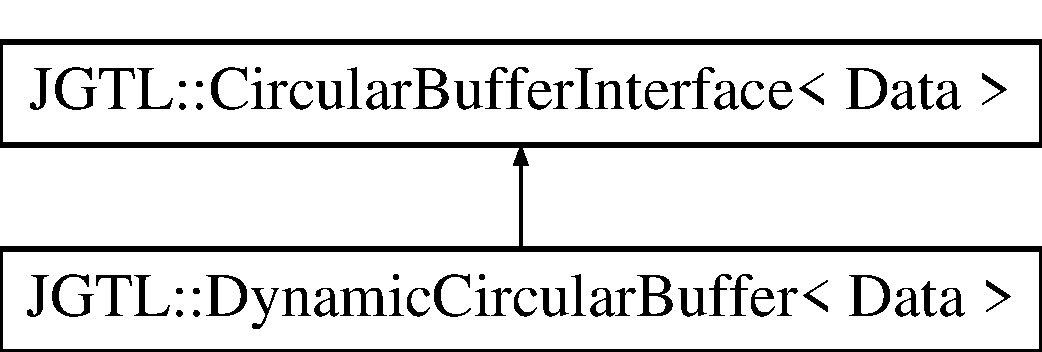
\includegraphics[height=2cm]{class_j_g_t_l_1_1_dynamic_circular_buffer}
\end{center}
\end{figure}
\subsection*{Public Member Functions}
\begin{CompactItemize}
\item 
\hyperlink{class_j_g_t_l_1_1_dynamic_circular_buffer_32e925536e7628b1e5a088300def83a5}{Dynamic\-Circular\-Buffer} (int initial\-Size=0)
\item 
\hyperlink{class_j_g_t_l_1_1_dynamic_circular_buffer_dff0297e4ca67ed7f7a9078579b2cc3f}{Dynamic\-Circular\-Buffer} (const \hyperlink{class_j_g_t_l_1_1_dynamic_circular_buffer}{Dynamic\-Circular\-Buffer} \&other)
\item 
const \hyperlink{class_j_g_t_l_1_1_dynamic_circular_buffer}{Dynamic\-Circular\-Buffer} \& \hyperlink{class_j_g_t_l_1_1_dynamic_circular_buffer_9a409b912e902f65ae09babd635b8d6e}{operator=} (const \hyperlink{class_j_g_t_l_1_1_dynamic_circular_buffer}{Dynamic\-Circular\-Buffer} \&other)
\item 
virtual \hyperlink{class_j_g_t_l_1_1_dynamic_circular_buffer_128034b920124c7f5d6d9e5da0e2050f}{$\sim$Dynamic\-Circular\-Buffer} ()
\item 
virtual bool \hyperlink{class_j_g_t_l_1_1_dynamic_circular_buffer_2ea8f91e985c5fec04eb8ef05898240a}{resize} (int new\-Size)
\end{CompactItemize}
\subsection*{Protected Member Functions}
\begin{CompactItemize}
\item 
void \hyperlink{class_j_g_t_l_1_1_dynamic_circular_buffer_5a81d3d91868e9c3ab1816583444984f}{copy\-From} (const \hyperlink{class_j_g_t_l_1_1_dynamic_circular_buffer}{Dynamic\-Circular\-Buffer} \&other)
\end{CompactItemize}


\subsection{Detailed Description}
\subsubsection*{template$<$class Data$>$ class JGTL::Dynamic\-Circular\-Buffer$<$ Data $>$}

The \hyperlink{class_j_g_t_l_1_1_dynamic_circular_buffer}{Dynamic\-Circular\-Buffer} Class handles a Circular Buffer. 

\begin{Desc}
\item[Author:]Jason Gauci \end{Desc}
\begin{Desc}
\item[Date:]2008 \end{Desc}




\subsection{Constructor \& Destructor Documentation}
\hypertarget{class_j_g_t_l_1_1_dynamic_circular_buffer_32e925536e7628b1e5a088300def83a5}{
\index{JGTL::DynamicCircularBuffer@{JGTL::Dynamic\-Circular\-Buffer}!DynamicCircularBuffer@{DynamicCircularBuffer}}
\index{DynamicCircularBuffer@{DynamicCircularBuffer}!JGTL::DynamicCircularBuffer@{JGTL::Dynamic\-Circular\-Buffer}}
\subsubsection[DynamicCircularBuffer]{\setlength{\rightskip}{0pt plus 5cm}template$<$class Data$>$ \hyperlink{class_j_g_t_l_1_1_dynamic_circular_buffer}{JGTL::Dynamic\-Circular\-Buffer}$<$ Data $>$::\hyperlink{class_j_g_t_l_1_1_dynamic_circular_buffer}{Dynamic\-Circular\-Buffer} (int {\em initial\-Size} = {\tt 0})\hspace{0.3cm}{\tt  \mbox{[}inline\mbox{]}}}}
\label{class_j_g_t_l_1_1_dynamic_circular_buffer_32e925536e7628b1e5a088300def83a5}


\hypertarget{class_j_g_t_l_1_1_dynamic_circular_buffer_dff0297e4ca67ed7f7a9078579b2cc3f}{
\index{JGTL::DynamicCircularBuffer@{JGTL::Dynamic\-Circular\-Buffer}!DynamicCircularBuffer@{DynamicCircularBuffer}}
\index{DynamicCircularBuffer@{DynamicCircularBuffer}!JGTL::DynamicCircularBuffer@{JGTL::Dynamic\-Circular\-Buffer}}
\subsubsection[DynamicCircularBuffer]{\setlength{\rightskip}{0pt plus 5cm}template$<$class Data$>$ \hyperlink{class_j_g_t_l_1_1_dynamic_circular_buffer}{JGTL::Dynamic\-Circular\-Buffer}$<$ Data $>$::\hyperlink{class_j_g_t_l_1_1_dynamic_circular_buffer}{Dynamic\-Circular\-Buffer} (const \hyperlink{class_j_g_t_l_1_1_dynamic_circular_buffer}{Dynamic\-Circular\-Buffer}$<$ Data $>$ \& {\em other})\hspace{0.3cm}{\tt  \mbox{[}inline\mbox{]}}}}
\label{class_j_g_t_l_1_1_dynamic_circular_buffer_dff0297e4ca67ed7f7a9078579b2cc3f}


\hypertarget{class_j_g_t_l_1_1_dynamic_circular_buffer_128034b920124c7f5d6d9e5da0e2050f}{
\index{JGTL::DynamicCircularBuffer@{JGTL::Dynamic\-Circular\-Buffer}!~DynamicCircularBuffer@{$\sim$DynamicCircularBuffer}}
\index{~DynamicCircularBuffer@{$\sim$DynamicCircularBuffer}!JGTL::DynamicCircularBuffer@{JGTL::Dynamic\-Circular\-Buffer}}
\subsubsection[$\sim$DynamicCircularBuffer]{\setlength{\rightskip}{0pt plus 5cm}template$<$class Data$>$ virtual \hyperlink{class_j_g_t_l_1_1_dynamic_circular_buffer}{JGTL::Dynamic\-Circular\-Buffer}$<$ Data $>$::$\sim$\hyperlink{class_j_g_t_l_1_1_dynamic_circular_buffer}{Dynamic\-Circular\-Buffer} ()\hspace{0.3cm}{\tt  \mbox{[}inline, virtual\mbox{]}}}}
\label{class_j_g_t_l_1_1_dynamic_circular_buffer_128034b920124c7f5d6d9e5da0e2050f}




\subsection{Member Function Documentation}
\hypertarget{class_j_g_t_l_1_1_dynamic_circular_buffer_9a409b912e902f65ae09babd635b8d6e}{
\index{JGTL::DynamicCircularBuffer@{JGTL::Dynamic\-Circular\-Buffer}!operator=@{operator=}}
\index{operator=@{operator=}!JGTL::DynamicCircularBuffer@{JGTL::Dynamic\-Circular\-Buffer}}
\subsubsection[operator=]{\setlength{\rightskip}{0pt plus 5cm}template$<$class Data$>$ const \hyperlink{class_j_g_t_l_1_1_dynamic_circular_buffer}{Dynamic\-Circular\-Buffer}\& \hyperlink{class_j_g_t_l_1_1_dynamic_circular_buffer}{JGTL::Dynamic\-Circular\-Buffer}$<$ Data $>$::operator= (const \hyperlink{class_j_g_t_l_1_1_dynamic_circular_buffer}{Dynamic\-Circular\-Buffer}$<$ Data $>$ \& {\em other})\hspace{0.3cm}{\tt  \mbox{[}inline\mbox{]}}}}
\label{class_j_g_t_l_1_1_dynamic_circular_buffer_9a409b912e902f65ae09babd635b8d6e}


\hypertarget{class_j_g_t_l_1_1_dynamic_circular_buffer_2ea8f91e985c5fec04eb8ef05898240a}{
\index{JGTL::DynamicCircularBuffer@{JGTL::Dynamic\-Circular\-Buffer}!resize@{resize}}
\index{resize@{resize}!JGTL::DynamicCircularBuffer@{JGTL::Dynamic\-Circular\-Buffer}}
\subsubsection[resize]{\setlength{\rightskip}{0pt plus 5cm}template$<$class Data$>$ virtual bool \hyperlink{class_j_g_t_l_1_1_dynamic_circular_buffer}{JGTL::Dynamic\-Circular\-Buffer}$<$ Data $>$::resize (int {\em new\-Size})\hspace{0.3cm}{\tt  \mbox{[}inline, virtual\mbox{]}}}}
\label{class_j_g_t_l_1_1_dynamic_circular_buffer_2ea8f91e985c5fec04eb8ef05898240a}




Implements \hyperlink{class_j_g_t_l_1_1_circular_buffer_interface_c6976a1811fdeb5b1810e379022f67ba}{JGTL::Circular\-Buffer\-Interface$<$ Data $>$}.\hypertarget{class_j_g_t_l_1_1_dynamic_circular_buffer_5a81d3d91868e9c3ab1816583444984f}{
\index{JGTL::DynamicCircularBuffer@{JGTL::Dynamic\-Circular\-Buffer}!copyFrom@{copyFrom}}
\index{copyFrom@{copyFrom}!JGTL::DynamicCircularBuffer@{JGTL::Dynamic\-Circular\-Buffer}}
\subsubsection[copyFrom]{\setlength{\rightskip}{0pt plus 5cm}template$<$class Data$>$ void \hyperlink{class_j_g_t_l_1_1_dynamic_circular_buffer}{JGTL::Dynamic\-Circular\-Buffer}$<$ Data $>$::copy\-From (const \hyperlink{class_j_g_t_l_1_1_dynamic_circular_buffer}{Dynamic\-Circular\-Buffer}$<$ Data $>$ \& {\em other})\hspace{0.3cm}{\tt  \mbox{[}inline, protected\mbox{]}}}}
\label{class_j_g_t_l_1_1_dynamic_circular_buffer_5a81d3d91868e9c3ab1816583444984f}




The documentation for this class was generated from the following file:\begin{CompactItemize}
\item 
\hyperlink{_j_g_t_l___dynamic_circular_buffer_8h}{JGTL\_\-Dynamic\-Circular\-Buffer.h}\end{CompactItemize}

\hypertarget{class_j_g_t_l_1_1_dynamic_pool_map}{
\section{JGTL::Dynamic\-Pool\-Map$<$ Key, Data $>$ Class Template Reference}
\label{class_j_g_t_l_1_1_dynamic_pool_map}\index{JGTL::DynamicPoolMap@{JGTL::DynamicPoolMap}}
}
The \hyperlink{class_j_g_t_l_1_1_dynamic_pool_map}{Dynamic\-Pool\-Map} Class is a resizable array-based associative map structure.  


{\tt \#include $<$JGTL\_\-Dynamic\-Pool\-Map.h$>$}

Inheritance diagram for JGTL::Dynamic\-Pool\-Map$<$ Key, Data $>$::\begin{figure}[H]
\begin{center}
\leavevmode
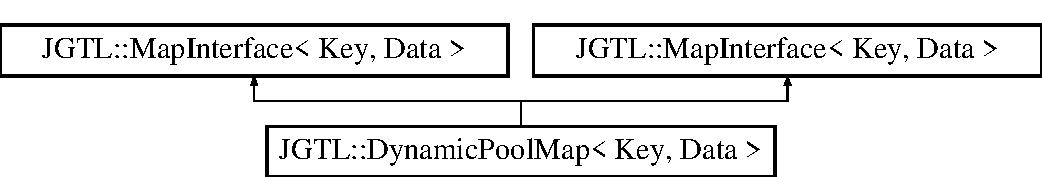
\includegraphics[height=2cm]{class_j_g_t_l_1_1_dynamic_pool_map}
\end{center}
\end{figure}
\subsection*{Public Member Functions}
\begin{CompactItemize}
\item 
\hyperlink{class_j_g_t_l_1_1_dynamic_pool_map_07c6425b3ff8be9bb668c187f6431b76}{Dynamic\-Pool\-Map} ()
\item 
\hyperlink{class_j_g_t_l_1_1_dynamic_pool_map_9735fb05911155de59c894f5074d7c34}{Dynamic\-Pool\-Map} (int \_\-capacity)
\item 
\hyperlink{class_j_g_t_l_1_1_dynamic_pool_map_309ac93775245116f166ac406fc192bd}{Dynamic\-Pool\-Map} (const \hyperlink{class_j_g_t_l_1_1_dynamic_pool_map}{Dynamic\-Pool\-Map} \&other)
\item 
const \hyperlink{class_j_g_t_l_1_1_dynamic_pool_map}{Dynamic\-Pool\-Map} \& \hyperlink{class_j_g_t_l_1_1_dynamic_pool_map_36d6be1323ed844a5d93ddf9814cc059}{operator=} (const \hyperlink{class_j_g_t_l_1_1_dynamic_pool_map}{Dynamic\-Pool\-Map} \&other)
\item 
virtual \hyperlink{class_j_g_t_l_1_1_dynamic_pool_map_b833361ff8ae724639fb0d4ed9e6392f}{$\sim$Dynamic\-Pool\-Map} ()
\item 
virtual bool \hyperlink{class_j_g_t_l_1_1_dynamic_pool_map_236509cad797d15cbed5e09adf356a04}{resize} (int new\-Size)
\item 
\hyperlink{class_j_g_t_l_1_1_dynamic_pool_map_07c6425b3ff8be9bb668c187f6431b76}{Dynamic\-Pool\-Map} ()
\item 
\hyperlink{class_j_g_t_l_1_1_dynamic_pool_map_309ac93775245116f166ac406fc192bd}{Dynamic\-Pool\-Map} (const \hyperlink{class_j_g_t_l_1_1_dynamic_pool_map}{Dynamic\-Pool\-Map} \&other)
\item 
const \hyperlink{class_j_g_t_l_1_1_dynamic_pool_map}{Dynamic\-Pool\-Map} \& \hyperlink{class_j_g_t_l_1_1_dynamic_pool_map_36d6be1323ed844a5d93ddf9814cc059}{operator=} (const \hyperlink{class_j_g_t_l_1_1_dynamic_pool_map}{Dynamic\-Pool\-Map} \&other)
\item 
virtual void \hyperlink{class_j_g_t_l_1_1_dynamic_pool_map_bce0771b0a4cc6238e7e3e24f5ec3bf0}{copy\-From} (const \hyperlink{class_j_g_t_l_1_1_dynamic_pool_map}{Dynamic\-Pool\-Map} \&other)
\item 
virtual \hyperlink{class_j_g_t_l_1_1_dynamic_pool_map_b833361ff8ae724639fb0d4ed9e6392f}{$\sim$Dynamic\-Pool\-Map} ()
\item 
virtual bool \hyperlink{class_j_g_t_l_1_1_dynamic_pool_map_28192d8477398c5a94b3ca80fc366076}{reserve} (int new\-Size)
\end{CompactItemize}
\subsection*{Protected Member Functions}
\begin{CompactItemize}
\item 
virtual void \hyperlink{class_j_g_t_l_1_1_dynamic_pool_map_bce0771b0a4cc6238e7e3e24f5ec3bf0}{copy\-From} (const \hyperlink{class_j_g_t_l_1_1_dynamic_pool_map}{Dynamic\-Pool\-Map} \&other)
\end{CompactItemize}


\subsection{Detailed Description}
\subsubsection*{template$<$class Key, class Data$>$ class JGTL::Dynamic\-Pool\-Map$<$ Key, Data $>$}

The \hyperlink{class_j_g_t_l_1_1_dynamic_pool_map}{Dynamic\-Pool\-Map} Class is a resizable array-based associative map structure. 

\begin{Desc}
\item[Author:]Jason Gauci \end{Desc}
\begin{Desc}
\item[Date:]2008 \end{Desc}




\subsection{Constructor \& Destructor Documentation}
\hypertarget{class_j_g_t_l_1_1_dynamic_pool_map_07c6425b3ff8be9bb668c187f6431b76}{
\index{JGTL::DynamicPoolMap@{JGTL::Dynamic\-Pool\-Map}!DynamicPoolMap@{DynamicPoolMap}}
\index{DynamicPoolMap@{DynamicPoolMap}!JGTL::DynamicPoolMap@{JGTL::Dynamic\-Pool\-Map}}
\subsubsection[DynamicPoolMap]{\setlength{\rightskip}{0pt plus 5cm}template$<$class Key, class Data$>$ \hyperlink{class_j_g_t_l_1_1_dynamic_pool_map}{JGTL::Dynamic\-Pool\-Map}$<$ Key, Data $>$::\hyperlink{class_j_g_t_l_1_1_dynamic_pool_map}{Dynamic\-Pool\-Map} ()\hspace{0.3cm}{\tt  \mbox{[}inline\mbox{]}}}}
\label{class_j_g_t_l_1_1_dynamic_pool_map_07c6425b3ff8be9bb668c187f6431b76}


\hypertarget{class_j_g_t_l_1_1_dynamic_pool_map_9735fb05911155de59c894f5074d7c34}{
\index{JGTL::DynamicPoolMap@{JGTL::Dynamic\-Pool\-Map}!DynamicPoolMap@{DynamicPoolMap}}
\index{DynamicPoolMap@{DynamicPoolMap}!JGTL::DynamicPoolMap@{JGTL::Dynamic\-Pool\-Map}}
\subsubsection[DynamicPoolMap]{\setlength{\rightskip}{0pt plus 5cm}template$<$class Key, class Data$>$ \hyperlink{class_j_g_t_l_1_1_dynamic_pool_map}{JGTL::Dynamic\-Pool\-Map}$<$ Key, Data $>$::\hyperlink{class_j_g_t_l_1_1_dynamic_pool_map}{Dynamic\-Pool\-Map} (int {\em \_\-capacity})\hspace{0.3cm}{\tt  \mbox{[}inline\mbox{]}}}}
\label{class_j_g_t_l_1_1_dynamic_pool_map_9735fb05911155de59c894f5074d7c34}


\hypertarget{class_j_g_t_l_1_1_dynamic_pool_map_309ac93775245116f166ac406fc192bd}{
\index{JGTL::DynamicPoolMap@{JGTL::Dynamic\-Pool\-Map}!DynamicPoolMap@{DynamicPoolMap}}
\index{DynamicPoolMap@{DynamicPoolMap}!JGTL::DynamicPoolMap@{JGTL::Dynamic\-Pool\-Map}}
\subsubsection[DynamicPoolMap]{\setlength{\rightskip}{0pt plus 5cm}template$<$class Key, class Data$>$ \hyperlink{class_j_g_t_l_1_1_dynamic_pool_map}{JGTL::Dynamic\-Pool\-Map}$<$ Key, Data $>$::\hyperlink{class_j_g_t_l_1_1_dynamic_pool_map}{Dynamic\-Pool\-Map} (const \hyperlink{class_j_g_t_l_1_1_dynamic_pool_map}{Dynamic\-Pool\-Map}$<$ Key, Data $>$ \& {\em other})\hspace{0.3cm}{\tt  \mbox{[}inline\mbox{]}}}}
\label{class_j_g_t_l_1_1_dynamic_pool_map_309ac93775245116f166ac406fc192bd}


\hypertarget{class_j_g_t_l_1_1_dynamic_pool_map_b833361ff8ae724639fb0d4ed9e6392f}{
\index{JGTL::DynamicPoolMap@{JGTL::Dynamic\-Pool\-Map}!~DynamicPoolMap@{$\sim$DynamicPoolMap}}
\index{~DynamicPoolMap@{$\sim$DynamicPoolMap}!JGTL::DynamicPoolMap@{JGTL::Dynamic\-Pool\-Map}}
\subsubsection[$\sim$DynamicPoolMap]{\setlength{\rightskip}{0pt plus 5cm}template$<$class Key, class Data$>$ virtual \hyperlink{class_j_g_t_l_1_1_dynamic_pool_map}{JGTL::Dynamic\-Pool\-Map}$<$ Key, Data $>$::$\sim$\hyperlink{class_j_g_t_l_1_1_dynamic_pool_map}{Dynamic\-Pool\-Map} ()\hspace{0.3cm}{\tt  \mbox{[}inline, virtual\mbox{]}}}}
\label{class_j_g_t_l_1_1_dynamic_pool_map_b833361ff8ae724639fb0d4ed9e6392f}


\hypertarget{class_j_g_t_l_1_1_dynamic_pool_map_07c6425b3ff8be9bb668c187f6431b76}{
\index{JGTL::DynamicPoolMap@{JGTL::Dynamic\-Pool\-Map}!DynamicPoolMap@{DynamicPoolMap}}
\index{DynamicPoolMap@{DynamicPoolMap}!JGTL::DynamicPoolMap@{JGTL::Dynamic\-Pool\-Map}}
\subsubsection[DynamicPoolMap]{\setlength{\rightskip}{0pt plus 5cm}template$<$class Key, class Data$>$ \hyperlink{class_j_g_t_l_1_1_dynamic_pool_map}{JGTL::Dynamic\-Pool\-Map}$<$ Key, Data $>$::\hyperlink{class_j_g_t_l_1_1_dynamic_pool_map}{Dynamic\-Pool\-Map} ()\hspace{0.3cm}{\tt  \mbox{[}inline\mbox{]}}}}
\label{class_j_g_t_l_1_1_dynamic_pool_map_07c6425b3ff8be9bb668c187f6431b76}


\hypertarget{class_j_g_t_l_1_1_dynamic_pool_map_309ac93775245116f166ac406fc192bd}{
\index{JGTL::DynamicPoolMap@{JGTL::Dynamic\-Pool\-Map}!DynamicPoolMap@{DynamicPoolMap}}
\index{DynamicPoolMap@{DynamicPoolMap}!JGTL::DynamicPoolMap@{JGTL::Dynamic\-Pool\-Map}}
\subsubsection[DynamicPoolMap]{\setlength{\rightskip}{0pt plus 5cm}template$<$class Key, class Data$>$ \hyperlink{class_j_g_t_l_1_1_dynamic_pool_map}{JGTL::Dynamic\-Pool\-Map}$<$ Key, Data $>$::\hyperlink{class_j_g_t_l_1_1_dynamic_pool_map}{Dynamic\-Pool\-Map} (const \hyperlink{class_j_g_t_l_1_1_dynamic_pool_map}{Dynamic\-Pool\-Map}$<$ Key, Data $>$ \& {\em other})\hspace{0.3cm}{\tt  \mbox{[}inline\mbox{]}}}}
\label{class_j_g_t_l_1_1_dynamic_pool_map_309ac93775245116f166ac406fc192bd}


\hypertarget{class_j_g_t_l_1_1_dynamic_pool_map_b833361ff8ae724639fb0d4ed9e6392f}{
\index{JGTL::DynamicPoolMap@{JGTL::Dynamic\-Pool\-Map}!~DynamicPoolMap@{$\sim$DynamicPoolMap}}
\index{~DynamicPoolMap@{$\sim$DynamicPoolMap}!JGTL::DynamicPoolMap@{JGTL::Dynamic\-Pool\-Map}}
\subsubsection[$\sim$DynamicPoolMap]{\setlength{\rightskip}{0pt plus 5cm}template$<$class Key, class Data$>$ virtual \hyperlink{class_j_g_t_l_1_1_dynamic_pool_map}{JGTL::Dynamic\-Pool\-Map}$<$ Key, Data $>$::$\sim$\hyperlink{class_j_g_t_l_1_1_dynamic_pool_map}{Dynamic\-Pool\-Map} ()\hspace{0.3cm}{\tt  \mbox{[}inline, virtual\mbox{]}}}}
\label{class_j_g_t_l_1_1_dynamic_pool_map_b833361ff8ae724639fb0d4ed9e6392f}




\subsection{Member Function Documentation}
\hypertarget{class_j_g_t_l_1_1_dynamic_pool_map_36d6be1323ed844a5d93ddf9814cc059}{
\index{JGTL::DynamicPoolMap@{JGTL::Dynamic\-Pool\-Map}!operator=@{operator=}}
\index{operator=@{operator=}!JGTL::DynamicPoolMap@{JGTL::Dynamic\-Pool\-Map}}
\subsubsection[operator=]{\setlength{\rightskip}{0pt plus 5cm}template$<$class Key, class Data$>$ const \hyperlink{class_j_g_t_l_1_1_dynamic_pool_map}{Dynamic\-Pool\-Map}\& \hyperlink{class_j_g_t_l_1_1_dynamic_pool_map}{JGTL::Dynamic\-Pool\-Map}$<$ Key, Data $>$::operator= (const \hyperlink{class_j_g_t_l_1_1_dynamic_pool_map}{Dynamic\-Pool\-Map}$<$ Key, Data $>$ \& {\em other})\hspace{0.3cm}{\tt  \mbox{[}inline\mbox{]}}}}
\label{class_j_g_t_l_1_1_dynamic_pool_map_36d6be1323ed844a5d93ddf9814cc059}


\hypertarget{class_j_g_t_l_1_1_dynamic_pool_map_236509cad797d15cbed5e09adf356a04}{
\index{JGTL::DynamicPoolMap@{JGTL::Dynamic\-Pool\-Map}!resize@{resize}}
\index{resize@{resize}!JGTL::DynamicPoolMap@{JGTL::Dynamic\-Pool\-Map}}
\subsubsection[resize]{\setlength{\rightskip}{0pt plus 5cm}template$<$class Key, class Data$>$ virtual bool \hyperlink{class_j_g_t_l_1_1_dynamic_pool_map}{JGTL::Dynamic\-Pool\-Map}$<$ Key, Data $>$::resize (int {\em new\-Size})\hspace{0.3cm}{\tt  \mbox{[}inline, virtual\mbox{]}}}}
\label{class_j_g_t_l_1_1_dynamic_pool_map_236509cad797d15cbed5e09adf356a04}




Implements \hyperlink{class_j_g_t_l_1_1_map_interface_177b75de36104c54e53080db65b777a2}{JGTL::Map\-Interface$<$ Key, Data $>$}.\hypertarget{class_j_g_t_l_1_1_dynamic_pool_map_bce0771b0a4cc6238e7e3e24f5ec3bf0}{
\index{JGTL::DynamicPoolMap@{JGTL::Dynamic\-Pool\-Map}!copyFrom@{copyFrom}}
\index{copyFrom@{copyFrom}!JGTL::DynamicPoolMap@{JGTL::Dynamic\-Pool\-Map}}
\subsubsection[copyFrom]{\setlength{\rightskip}{0pt plus 5cm}template$<$class Key, class Data$>$ virtual void \hyperlink{class_j_g_t_l_1_1_dynamic_pool_map}{JGTL::Dynamic\-Pool\-Map}$<$ Key, Data $>$::copy\-From (const \hyperlink{class_j_g_t_l_1_1_dynamic_pool_map}{Dynamic\-Pool\-Map}$<$ Key, Data $>$ \& {\em other})\hspace{0.3cm}{\tt  \mbox{[}inline, protected, virtual\mbox{]}}}}
\label{class_j_g_t_l_1_1_dynamic_pool_map_bce0771b0a4cc6238e7e3e24f5ec3bf0}


\hypertarget{class_j_g_t_l_1_1_dynamic_pool_map_36d6be1323ed844a5d93ddf9814cc059}{
\index{JGTL::DynamicPoolMap@{JGTL::Dynamic\-Pool\-Map}!operator=@{operator=}}
\index{operator=@{operator=}!JGTL::DynamicPoolMap@{JGTL::Dynamic\-Pool\-Map}}
\subsubsection[operator=]{\setlength{\rightskip}{0pt plus 5cm}template$<$class Key, class Data$>$ const \hyperlink{class_j_g_t_l_1_1_dynamic_pool_map}{Dynamic\-Pool\-Map}\& \hyperlink{class_j_g_t_l_1_1_dynamic_pool_map}{JGTL::Dynamic\-Pool\-Map}$<$ Key, Data $>$::operator= (const \hyperlink{class_j_g_t_l_1_1_dynamic_pool_map}{Dynamic\-Pool\-Map}$<$ Key, Data $>$ \& {\em other})\hspace{0.3cm}{\tt  \mbox{[}inline\mbox{]}}}}
\label{class_j_g_t_l_1_1_dynamic_pool_map_36d6be1323ed844a5d93ddf9814cc059}


\hypertarget{class_j_g_t_l_1_1_dynamic_pool_map_bce0771b0a4cc6238e7e3e24f5ec3bf0}{
\index{JGTL::DynamicPoolMap@{JGTL::Dynamic\-Pool\-Map}!copyFrom@{copyFrom}}
\index{copyFrom@{copyFrom}!JGTL::DynamicPoolMap@{JGTL::Dynamic\-Pool\-Map}}
\subsubsection[copyFrom]{\setlength{\rightskip}{0pt plus 5cm}template$<$class Key, class Data$>$ virtual void \hyperlink{class_j_g_t_l_1_1_dynamic_pool_map}{JGTL::Dynamic\-Pool\-Map}$<$ Key, Data $>$::copy\-From (const \hyperlink{class_j_g_t_l_1_1_dynamic_pool_map}{Dynamic\-Pool\-Map}$<$ Key, Data $>$ \& {\em other})\hspace{0.3cm}{\tt  \mbox{[}inline, virtual\mbox{]}}}}
\label{class_j_g_t_l_1_1_dynamic_pool_map_bce0771b0a4cc6238e7e3e24f5ec3bf0}


\hypertarget{class_j_g_t_l_1_1_dynamic_pool_map_28192d8477398c5a94b3ca80fc366076}{
\index{JGTL::DynamicPoolMap@{JGTL::Dynamic\-Pool\-Map}!reserve@{reserve}}
\index{reserve@{reserve}!JGTL::DynamicPoolMap@{JGTL::Dynamic\-Pool\-Map}}
\subsubsection[reserve]{\setlength{\rightskip}{0pt plus 5cm}template$<$class Key, class Data$>$ virtual bool \hyperlink{class_j_g_t_l_1_1_dynamic_pool_map}{JGTL::Dynamic\-Pool\-Map}$<$ Key, Data $>$::reserve (int {\em new\-Size})\hspace{0.3cm}{\tt  \mbox{[}inline, virtual\mbox{]}}}}
\label{class_j_g_t_l_1_1_dynamic_pool_map_28192d8477398c5a94b3ca80fc366076}




Reimplemented from \hyperlink{class_j_g_t_l_1_1_map_interface_d5d7c32e4e413ef6fcd93ca53951ecf8}{JGTL::Map\-Interface$<$ Key, Data $>$}.

The documentation for this class was generated from the following files:\begin{CompactItemize}
\item 
\hyperlink{_j_g_t_l___dynamic_pool_map_8h}{JGTL\_\-Dynamic\-Pool\-Map.h}\item 
\hyperlink{_j_g_t_l___unordered_dynamic_pool_map_8h}{JGTL\_\-Unordered\-Dynamic\-Pool\-Map.h}\end{CompactItemize}

\hypertarget{class_j_g_t_l_1_1_dynamic_pool_set}{
\section{JGTL::Dynamic\-Pool\-Set$<$ Data $>$ Class Template Reference}
\label{class_j_g_t_l_1_1_dynamic_pool_set}\index{JGTL::DynamicPoolSet@{JGTL::DynamicPoolSet}}
}
{\tt \#include $<$JGTL\_\-Dynamic\-Pool\-Set.h$>$}

Inheritance diagram for JGTL::Dynamic\-Pool\-Set$<$ Data $>$::\begin{figure}[H]
\begin{center}
\leavevmode
\includegraphics[height=2cm]{class_j_g_t_l_1_1_dynamic_pool_set}
\end{center}
\end{figure}
\subsection*{Public Member Functions}
\begin{CompactItemize}
\item 
\hyperlink{class_j_g_t_l_1_1_dynamic_pool_set_7782c2398e24e10e1a4e4b6571740fb2}{Dynamic\-Pool\-Set} ()
\item 
\hyperlink{class_j_g_t_l_1_1_dynamic_pool_set_d079124f4b30c87f7bb102f306f7c7ae}{Dynamic\-Pool\-Set} (const \hyperlink{class_j_g_t_l_1_1_dynamic_pool_set}{Dynamic\-Pool\-Set}$<$ Data $>$ \&other)
\item 
const \hyperlink{class_j_g_t_l_1_1_dynamic_pool_set}{Dynamic\-Pool\-Set} \& \hyperlink{class_j_g_t_l_1_1_dynamic_pool_set_dd18f7df0d3a13b31f53a13a755cd729}{operator=} (const \hyperlink{class_j_g_t_l_1_1_dynamic_pool_set}{Dynamic\-Pool\-Set}$<$ Data $>$ \&other)
\item 
void \hyperlink{class_j_g_t_l_1_1_dynamic_pool_set_b3dbb5689852c8b7305bb5e51b6f0a5f}{copy\-From} (const \hyperlink{class_j_g_t_l_1_1_dynamic_pool_set}{Dynamic\-Pool\-Set} \&other)
\item 
virtual \hyperlink{class_j_g_t_l_1_1_dynamic_pool_set_61626b46e2bd79d1c188ff76725ac50c}{$\sim$Dynamic\-Pool\-Set} ()
\item 
bool \hyperlink{class_j_g_t_l_1_1_dynamic_pool_set_6b6a5c1f4536294a29afaa22417c761a}{operator==} (const \hyperlink{class_j_g_t_l_1_1_dynamic_pool_set}{Dynamic\-Pool\-Set} \&other) const 
\item 
virtual bool \hyperlink{class_j_g_t_l_1_1_dynamic_pool_set_f9c2b0ebc042c33dca8fee5af6583446}{resize} (int new\-Size)
\end{CompactItemize}
\subsubsection*{template$<$class Data$>$ class JGTL::Dynamic\-Pool\-Set$<$ Data $>$}



\subsection{Constructor \& Destructor Documentation}
\hypertarget{class_j_g_t_l_1_1_dynamic_pool_set_7782c2398e24e10e1a4e4b6571740fb2}{
\index{JGTL::DynamicPoolSet@{JGTL::Dynamic\-Pool\-Set}!DynamicPoolSet@{DynamicPoolSet}}
\index{DynamicPoolSet@{DynamicPoolSet}!JGTL::DynamicPoolSet@{JGTL::Dynamic\-Pool\-Set}}
\subsubsection[DynamicPoolSet]{\setlength{\rightskip}{0pt plus 5cm}template$<$class Data$>$ \hyperlink{class_j_g_t_l_1_1_dynamic_pool_set}{JGTL::Dynamic\-Pool\-Set}$<$ Data $>$::\hyperlink{class_j_g_t_l_1_1_dynamic_pool_set}{Dynamic\-Pool\-Set} ()\hspace{0.3cm}{\tt  \mbox{[}inline\mbox{]}}}}
\label{class_j_g_t_l_1_1_dynamic_pool_set_7782c2398e24e10e1a4e4b6571740fb2}


\hypertarget{class_j_g_t_l_1_1_dynamic_pool_set_d079124f4b30c87f7bb102f306f7c7ae}{
\index{JGTL::DynamicPoolSet@{JGTL::Dynamic\-Pool\-Set}!DynamicPoolSet@{DynamicPoolSet}}
\index{DynamicPoolSet@{DynamicPoolSet}!JGTL::DynamicPoolSet@{JGTL::Dynamic\-Pool\-Set}}
\subsubsection[DynamicPoolSet]{\setlength{\rightskip}{0pt plus 5cm}template$<$class Data$>$ \hyperlink{class_j_g_t_l_1_1_dynamic_pool_set}{JGTL::Dynamic\-Pool\-Set}$<$ Data $>$::\hyperlink{class_j_g_t_l_1_1_dynamic_pool_set}{Dynamic\-Pool\-Set} (const \hyperlink{class_j_g_t_l_1_1_dynamic_pool_set}{Dynamic\-Pool\-Set}$<$ Data $>$ \& {\em other})\hspace{0.3cm}{\tt  \mbox{[}inline\mbox{]}}}}
\label{class_j_g_t_l_1_1_dynamic_pool_set_d079124f4b30c87f7bb102f306f7c7ae}


\hypertarget{class_j_g_t_l_1_1_dynamic_pool_set_61626b46e2bd79d1c188ff76725ac50c}{
\index{JGTL::DynamicPoolSet@{JGTL::Dynamic\-Pool\-Set}!~DynamicPoolSet@{$\sim$DynamicPoolSet}}
\index{~DynamicPoolSet@{$\sim$DynamicPoolSet}!JGTL::DynamicPoolSet@{JGTL::Dynamic\-Pool\-Set}}
\subsubsection[$\sim$DynamicPoolSet]{\setlength{\rightskip}{0pt plus 5cm}template$<$class Data$>$ virtual \hyperlink{class_j_g_t_l_1_1_dynamic_pool_set}{JGTL::Dynamic\-Pool\-Set}$<$ Data $>$::$\sim$\hyperlink{class_j_g_t_l_1_1_dynamic_pool_set}{Dynamic\-Pool\-Set} ()\hspace{0.3cm}{\tt  \mbox{[}inline, virtual\mbox{]}}}}
\label{class_j_g_t_l_1_1_dynamic_pool_set_61626b46e2bd79d1c188ff76725ac50c}




\subsection{Member Function Documentation}
\hypertarget{class_j_g_t_l_1_1_dynamic_pool_set_dd18f7df0d3a13b31f53a13a755cd729}{
\index{JGTL::DynamicPoolSet@{JGTL::Dynamic\-Pool\-Set}!operator=@{operator=}}
\index{operator=@{operator=}!JGTL::DynamicPoolSet@{JGTL::Dynamic\-Pool\-Set}}
\subsubsection[operator=]{\setlength{\rightskip}{0pt plus 5cm}template$<$class Data$>$ const \hyperlink{class_j_g_t_l_1_1_dynamic_pool_set}{Dynamic\-Pool\-Set}\& \hyperlink{class_j_g_t_l_1_1_dynamic_pool_set}{JGTL::Dynamic\-Pool\-Set}$<$ Data $>$::operator= (const \hyperlink{class_j_g_t_l_1_1_dynamic_pool_set}{Dynamic\-Pool\-Set}$<$ Data $>$ \& {\em other})\hspace{0.3cm}{\tt  \mbox{[}inline\mbox{]}}}}
\label{class_j_g_t_l_1_1_dynamic_pool_set_dd18f7df0d3a13b31f53a13a755cd729}


\hypertarget{class_j_g_t_l_1_1_dynamic_pool_set_b3dbb5689852c8b7305bb5e51b6f0a5f}{
\index{JGTL::DynamicPoolSet@{JGTL::Dynamic\-Pool\-Set}!copyFrom@{copyFrom}}
\index{copyFrom@{copyFrom}!JGTL::DynamicPoolSet@{JGTL::Dynamic\-Pool\-Set}}
\subsubsection[copyFrom]{\setlength{\rightskip}{0pt plus 5cm}template$<$class Data$>$ void \hyperlink{class_j_g_t_l_1_1_dynamic_pool_set}{JGTL::Dynamic\-Pool\-Set}$<$ Data $>$::copy\-From (const \hyperlink{class_j_g_t_l_1_1_dynamic_pool_set}{Dynamic\-Pool\-Set}$<$ Data $>$ \& {\em other})\hspace{0.3cm}{\tt  \mbox{[}inline\mbox{]}}}}
\label{class_j_g_t_l_1_1_dynamic_pool_set_b3dbb5689852c8b7305bb5e51b6f0a5f}


\hypertarget{class_j_g_t_l_1_1_dynamic_pool_set_6b6a5c1f4536294a29afaa22417c761a}{
\index{JGTL::DynamicPoolSet@{JGTL::Dynamic\-Pool\-Set}!operator==@{operator==}}
\index{operator==@{operator==}!JGTL::DynamicPoolSet@{JGTL::Dynamic\-Pool\-Set}}
\subsubsection[operator==]{\setlength{\rightskip}{0pt plus 5cm}template$<$class Data$>$ bool \hyperlink{class_j_g_t_l_1_1_dynamic_pool_set}{JGTL::Dynamic\-Pool\-Set}$<$ Data $>$::operator== (const \hyperlink{class_j_g_t_l_1_1_dynamic_pool_set}{Dynamic\-Pool\-Set}$<$ Data $>$ \& {\em other}) const\hspace{0.3cm}{\tt  \mbox{[}inline\mbox{]}}}}
\label{class_j_g_t_l_1_1_dynamic_pool_set_6b6a5c1f4536294a29afaa22417c761a}


\hypertarget{class_j_g_t_l_1_1_dynamic_pool_set_f9c2b0ebc042c33dca8fee5af6583446}{
\index{JGTL::DynamicPoolSet@{JGTL::Dynamic\-Pool\-Set}!resize@{resize}}
\index{resize@{resize}!JGTL::DynamicPoolSet@{JGTL::Dynamic\-Pool\-Set}}
\subsubsection[resize]{\setlength{\rightskip}{0pt plus 5cm}template$<$class Data$>$ virtual bool \hyperlink{class_j_g_t_l_1_1_dynamic_pool_set}{JGTL::Dynamic\-Pool\-Set}$<$ Data $>$::resize (int {\em new\-Size})\hspace{0.3cm}{\tt  \mbox{[}inline, virtual\mbox{]}}}}
\label{class_j_g_t_l_1_1_dynamic_pool_set_f9c2b0ebc042c33dca8fee5af6583446}




Reimplemented from \hyperlink{class_j_g_t_l_1_1_set_interface_136d868ffd3695632c16e4f88b84352b}{JGTL::Set\-Interface$<$ Data $>$}.

The documentation for this class was generated from the following file:\begin{CompactItemize}
\item 
\hyperlink{_j_g_t_l___dynamic_pool_set_8h}{JGTL\_\-Dynamic\-Pool\-Set.h}\end{CompactItemize}

\hypertarget{class_j_g_t_l_1_1_floating_units}{
\section{JGTL::Floating\-Units$<$ Value\-Type, SCALE\_\-NUMERATOR, SCALE\_\-DENOMINATOR $>$ Class Template Reference}
\label{class_j_g_t_l_1_1_floating_units}\index{JGTL::FloatingUnits@{JGTL::FloatingUnits}}
}
{\tt \#include $<$JGTL\_\-Floating\-Units.h$>$}

\subsection*{Public Member Functions}
\begin{CompactItemize}
\item 
\hyperlink{class_j_g_t_l_1_1_floating_units_4f7658a1fa622c855a6c5923eb5add64}{Floating\-Units} (Value\-Type \_\-value=0)
\item 
template$<$class Other\-Value\-Type, units\_\-internal\_\-ulong OTHERSCALE\_\-NUMERATOR, units\_\-internal\_\-ulong OTHERSCALE\_\-DENOMINATOR$>$ \hyperlink{class_j_g_t_l_1_1_floating_units_0a786872a5e5665fd87998c4df382753}{Floating\-Units} (const \hyperlink{class_j_g_t_l_1_1_floating_units}{Floating\-Units}$<$ Other\-Value\-Type, OTHERSCALE\_\-NUMERATOR, OTHERSCALE\_\-DENOMINATOR $>$ \&t)
\item 
template$<$class Other\-Value\-Type, units\_\-internal\_\-ulong OTHERSCALE\_\-NUMERATOR, units\_\-internal\_\-ulong OTHERSCALE\_\-DENOMINATOR$>$ const \hyperlink{class_j_g_t_l_1_1_floating_units}{Floating\-Units} \& \hyperlink{class_j_g_t_l_1_1_floating_units_0c909f9f4b76403e848172b65a0c418a}{operator=} (const \hyperlink{class_j_g_t_l_1_1_floating_units}{Floating\-Units}$<$ Other\-Value\-Type, OTHERSCALE\_\-NUMERATOR, OTHERSCALE\_\-DENOMINATOR $>$ \&t)
\item 
template$<$class Other\-Value\-Type, units\_\-internal\_\-ulong OTHERSCALE\_\-NUMERATOR, units\_\-internal\_\-ulong OTHERSCALE\_\-DENOMINATOR$>$ Value\-Type \hyperlink{class_j_g_t_l_1_1_floating_units_c7e85ddf1877abac6e7a77f035d68a1b}{change\-Scale} (const \hyperlink{class_j_g_t_l_1_1_floating_units}{Floating\-Units}$<$ Other\-Value\-Type, OTHERSCALE\_\-NUMERATOR, OTHERSCALE\_\-DENOMINATOR $>$ \&t)
\item 
virtual Value\-Type \hyperlink{class_j_g_t_l_1_1_floating_units_38ce55dd061c7b566f2a146ad062816a}{get\-Scale} () const
\item 
void \hyperlink{class_j_g_t_l_1_1_floating_units_b4f0691c805340b545251b6216a406f3}{set\-Value} (Value\-Type \_\-value)
\item 
Value\-Type \hyperlink{class_j_g_t_l_1_1_floating_units_0151027d566bdf3be45f2f8830d26664}{get\-Value} () const
\end{CompactItemize}
\subsection*{Protected Attributes}
\begin{CompactItemize}
\item 
Value\-Type \hyperlink{class_j_g_t_l_1_1_floating_units_5e84b8db278f0079f543818213b2bac5}{value}
\end{CompactItemize}
\subsubsection*{template$<$class Value\-Type, units\_\-internal\_\-ulong SCALE\_\-NUMERATOR, units\_\-internal\_\-ulong SCALE\_\-DENOMINATOR$>$ class JGTL::Floating\-Units$<$ Value\-Type, SCALE\_\-NUMERATOR, SCALE\_\-DENOMINATOR $>$}



\subsection{Constructor \& Destructor Documentation}
\hypertarget{class_j_g_t_l_1_1_floating_units_4f7658a1fa622c855a6c5923eb5add64}{
\index{JGTL::FloatingUnits@{JGTL::Floating\-Units}!FloatingUnits@{FloatingUnits}}
\index{FloatingUnits@{FloatingUnits}!JGTL::FloatingUnits@{JGTL::Floating\-Units}}
\subsubsection[FloatingUnits]{\setlength{\rightskip}{0pt plus 5cm}template$<$class Value\-Type, units\_\-internal\_\-ulong SCALE\_\-NUMERATOR, units\_\-internal\_\-ulong SCALE\_\-DENOMINATOR$>$ \hyperlink{class_j_g_t_l_1_1_floating_units}{JGTL::Floating\-Units}$<$ Value\-Type, SCALE\_\-NUMERATOR, SCALE\_\-DENOMINATOR $>$::\hyperlink{class_j_g_t_l_1_1_floating_units}{Floating\-Units} (Value\-Type {\em \_\-value} = {\tt 0})\hspace{0.3cm}{\tt  \mbox{[}inline\mbox{]}}}}
\label{class_j_g_t_l_1_1_floating_units_4f7658a1fa622c855a6c5923eb5add64}


\hypertarget{class_j_g_t_l_1_1_floating_units_0a786872a5e5665fd87998c4df382753}{
\index{JGTL::FloatingUnits@{JGTL::Floating\-Units}!FloatingUnits@{FloatingUnits}}
\index{FloatingUnits@{FloatingUnits}!JGTL::FloatingUnits@{JGTL::Floating\-Units}}
\subsubsection[FloatingUnits]{\setlength{\rightskip}{0pt plus 5cm}template$<$class Value\-Type, units\_\-internal\_\-ulong SCALE\_\-NUMERATOR, units\_\-internal\_\-ulong SCALE\_\-DENOMINATOR$>$ template$<$class Other\-Value\-Type, units\_\-internal\_\-ulong OTHERSCALE\_\-NUMERATOR, units\_\-internal\_\-ulong OTHERSCALE\_\-DENOMINATOR$>$ \hyperlink{class_j_g_t_l_1_1_floating_units}{JGTL::Floating\-Units}$<$ Value\-Type, SCALE\_\-NUMERATOR, SCALE\_\-DENOMINATOR $>$::\hyperlink{class_j_g_t_l_1_1_floating_units}{Floating\-Units} (const \hyperlink{class_j_g_t_l_1_1_floating_units}{Floating\-Units}$<$ Other\-Value\-Type, OTHERSCALE\_\-NUMERATOR, OTHERSCALE\_\-DENOMINATOR $>$ \& {\em t})\hspace{0.3cm}{\tt  \mbox{[}inline\mbox{]}}}}
\label{class_j_g_t_l_1_1_floating_units_0a786872a5e5665fd87998c4df382753}




\subsection{Member Function Documentation}
\hypertarget{class_j_g_t_l_1_1_floating_units_0c909f9f4b76403e848172b65a0c418a}{
\index{JGTL::FloatingUnits@{JGTL::Floating\-Units}!operator=@{operator=}}
\index{operator=@{operator=}!JGTL::FloatingUnits@{JGTL::Floating\-Units}}
\subsubsection[operator=]{\setlength{\rightskip}{0pt plus 5cm}template$<$class Value\-Type, units\_\-internal\_\-ulong SCALE\_\-NUMERATOR, units\_\-internal\_\-ulong SCALE\_\-DENOMINATOR$>$ template$<$class Other\-Value\-Type, units\_\-internal\_\-ulong OTHERSCALE\_\-NUMERATOR, units\_\-internal\_\-ulong OTHERSCALE\_\-DENOMINATOR$>$ const \hyperlink{class_j_g_t_l_1_1_floating_units}{Floating\-Units}\& \hyperlink{class_j_g_t_l_1_1_floating_units}{JGTL::Floating\-Units}$<$ Value\-Type, SCALE\_\-NUMERATOR, SCALE\_\-DENOMINATOR $>$::operator= (const \hyperlink{class_j_g_t_l_1_1_floating_units}{Floating\-Units}$<$ Other\-Value\-Type, OTHERSCALE\_\-NUMERATOR, OTHERSCALE\_\-DENOMINATOR $>$ \& {\em t})\hspace{0.3cm}{\tt  \mbox{[}inline\mbox{]}}}}
\label{class_j_g_t_l_1_1_floating_units_0c909f9f4b76403e848172b65a0c418a}


\hypertarget{class_j_g_t_l_1_1_floating_units_c7e85ddf1877abac6e7a77f035d68a1b}{
\index{JGTL::FloatingUnits@{JGTL::Floating\-Units}!changeScale@{changeScale}}
\index{changeScale@{changeScale}!JGTL::FloatingUnits@{JGTL::Floating\-Units}}
\subsubsection[changeScale]{\setlength{\rightskip}{0pt plus 5cm}template$<$class Value\-Type, units\_\-internal\_\-ulong SCALE\_\-NUMERATOR, units\_\-internal\_\-ulong SCALE\_\-DENOMINATOR$>$ template$<$class Other\-Value\-Type, units\_\-internal\_\-ulong OTHERSCALE\_\-NUMERATOR, units\_\-internal\_\-ulong OTHERSCALE\_\-DENOMINATOR$>$ Value\-Type \hyperlink{class_j_g_t_l_1_1_floating_units}{JGTL::Floating\-Units}$<$ Value\-Type, SCALE\_\-NUMERATOR, SCALE\_\-DENOMINATOR $>$::change\-Scale (const \hyperlink{class_j_g_t_l_1_1_floating_units}{Floating\-Units}$<$ Other\-Value\-Type, OTHERSCALE\_\-NUMERATOR, OTHERSCALE\_\-DENOMINATOR $>$ \& {\em t})\hspace{0.3cm}{\tt  \mbox{[}inline\mbox{]}}}}
\label{class_j_g_t_l_1_1_floating_units_c7e85ddf1877abac6e7a77f035d68a1b}


\hypertarget{class_j_g_t_l_1_1_floating_units_38ce55dd061c7b566f2a146ad062816a}{
\index{JGTL::FloatingUnits@{JGTL::Floating\-Units}!getScale@{getScale}}
\index{getScale@{getScale}!JGTL::FloatingUnits@{JGTL::Floating\-Units}}
\subsubsection[getScale]{\setlength{\rightskip}{0pt plus 5cm}template$<$class Value\-Type, units\_\-internal\_\-ulong SCALE\_\-NUMERATOR, units\_\-internal\_\-ulong SCALE\_\-DENOMINATOR$>$ virtual Value\-Type \hyperlink{class_j_g_t_l_1_1_floating_units}{JGTL::Floating\-Units}$<$ Value\-Type, SCALE\_\-NUMERATOR, SCALE\_\-DENOMINATOR $>$::get\-Scale () const\hspace{0.3cm}{\tt  \mbox{[}inline, virtual\mbox{]}}}}
\label{class_j_g_t_l_1_1_floating_units_38ce55dd061c7b566f2a146ad062816a}


\hypertarget{class_j_g_t_l_1_1_floating_units_b4f0691c805340b545251b6216a406f3}{
\index{JGTL::FloatingUnits@{JGTL::Floating\-Units}!setValue@{setValue}}
\index{setValue@{setValue}!JGTL::FloatingUnits@{JGTL::Floating\-Units}}
\subsubsection[setValue]{\setlength{\rightskip}{0pt plus 5cm}template$<$class Value\-Type, units\_\-internal\_\-ulong SCALE\_\-NUMERATOR, units\_\-internal\_\-ulong SCALE\_\-DENOMINATOR$>$ void \hyperlink{class_j_g_t_l_1_1_floating_units}{JGTL::Floating\-Units}$<$ Value\-Type, SCALE\_\-NUMERATOR, SCALE\_\-DENOMINATOR $>$::set\-Value (Value\-Type {\em \_\-value})\hspace{0.3cm}{\tt  \mbox{[}inline\mbox{]}}}}
\label{class_j_g_t_l_1_1_floating_units_b4f0691c805340b545251b6216a406f3}


\hypertarget{class_j_g_t_l_1_1_floating_units_0151027d566bdf3be45f2f8830d26664}{
\index{JGTL::FloatingUnits@{JGTL::Floating\-Units}!getValue@{getValue}}
\index{getValue@{getValue}!JGTL::FloatingUnits@{JGTL::Floating\-Units}}
\subsubsection[getValue]{\setlength{\rightskip}{0pt plus 5cm}template$<$class Value\-Type, units\_\-internal\_\-ulong SCALE\_\-NUMERATOR, units\_\-internal\_\-ulong SCALE\_\-DENOMINATOR$>$ Value\-Type \hyperlink{class_j_g_t_l_1_1_floating_units}{JGTL::Floating\-Units}$<$ Value\-Type, SCALE\_\-NUMERATOR, SCALE\_\-DENOMINATOR $>$::get\-Value () const\hspace{0.3cm}{\tt  \mbox{[}inline\mbox{]}}}}
\label{class_j_g_t_l_1_1_floating_units_0151027d566bdf3be45f2f8830d26664}




\subsection{Member Data Documentation}
\hypertarget{class_j_g_t_l_1_1_floating_units_5e84b8db278f0079f543818213b2bac5}{
\index{JGTL::FloatingUnits@{JGTL::Floating\-Units}!value@{value}}
\index{value@{value}!JGTL::FloatingUnits@{JGTL::Floating\-Units}}
\subsubsection[value]{\setlength{\rightskip}{0pt plus 5cm}template$<$class Value\-Type, units\_\-internal\_\-ulong SCALE\_\-NUMERATOR, units\_\-internal\_\-ulong SCALE\_\-DENOMINATOR$>$ Value\-Type \hyperlink{class_j_g_t_l_1_1_floating_units}{JGTL::Floating\-Units}$<$ Value\-Type, SCALE\_\-NUMERATOR, SCALE\_\-DENOMINATOR $>$::\hyperlink{class_j_g_t_l_1_1_floating_units_5e84b8db278f0079f543818213b2bac5}{value}\hspace{0.3cm}{\tt  \mbox{[}protected\mbox{]}}}}
\label{class_j_g_t_l_1_1_floating_units_5e84b8db278f0079f543818213b2bac5}




The documentation for this class was generated from the following file:\begin{CompactItemize}
\item 
\hyperlink{_j_g_t_l___floating_units_8h}{JGTL\_\-Floating\-Units.h}\end{CompactItemize}

\hypertarget{class_j_g_t_l_1_1_hex_tree}{
\section{JGTL::Hex\-Tree$<$ T $>$ Class Template Reference}
\label{class_j_g_t_l_1_1_hex_tree}\index{JGTL::HexTree@{JGTL::HexTree}}
}
{\tt \#include $<$JGTL\_\-Hex\-Tree.h$>$}

\subsection*{Public Member Functions}
\begin{CompactItemize}
\item 
\hyperlink{class_j_g_t_l_1_1_hex_tree_0bc0009b14ba1373be655f7f8939759b}{Hex\-Tree} (int \_\-size=16, T default\-Value=(T) 0)
\item 
\hyperlink{class_j_g_t_l_1_1_hex_tree_b33bd761f532e8a9489269bbb9816cc5}{Hex\-Tree} (const \hyperlink{class_j_g_t_l_1_1_hex_tree}{Hex\-Tree}$<$ T $>$ \&other)
\item 
\hyperlink{class_j_g_t_l_1_1_hex_tree_d378b61bdb0638b99d2afd06cf90a62e}{$\sim$Hex\-Tree} ()
\item 
\hyperlink{class_j_g_t_l_1_1_hex_tree}{Hex\-Tree}$<$ T $>$ \& \hyperlink{class_j_g_t_l_1_1_hex_tree_511cd2289f7aced36c88122de0b41dbc}{operator=} (const \hyperlink{class_j_g_t_l_1_1_hex_tree}{Hex\-Tree}$<$ T $>$ \&other)
\item 
void \hyperlink{class_j_g_t_l_1_1_hex_tree_6d8486ed19b1f07ae74b85fcb6bc6969}{copy\-From} (const \hyperlink{class_j_g_t_l_1_1_hex_tree}{Hex\-Tree}$<$ T $>$ \&other)
\item 
T \hyperlink{class_j_g_t_l_1_1_hex_tree_72f9d55be8d485f8ef551d6c27aab7d7}{get\-Value} (const \hyperlink{class_j_g_t_l_1_1_vector4}{Vector4}$<$ int $>$ \&location) const
\item 
T \hyperlink{class_j_g_t_l_1_1_hex_tree_1d6ec3d8be42e25c77209fab1b350d43}{get\-Value} (int x1, int y1, int x2, int y2) const
\item 
void \hyperlink{class_j_g_t_l_1_1_hex_tree_e91ed4c6f6373541acc8dec5b82c91b4}{set\-Value} (const \hyperlink{class_j_g_t_l_1_1_vector4}{Vector4}$<$ int $>$ \&location, T value)
\item 
void \hyperlink{class_j_g_t_l_1_1_hex_tree_e39f7e05c965191d3809649ea4f7aad9}{set\-Value} (int x1, int y1, int x2, int y2, T value)
\item 
void \hyperlink{class_j_g_t_l_1_1_hex_tree_d98751804b80105248de750d25732c6d}{set\-All} (T value)
\item 
void \hyperlink{class_j_g_t_l_1_1_hex_tree_6d57b2b70e4fc6bac53e7fe193b95bdf}{display} () const
\item 
T \hyperlink{class_j_g_t_l_1_1_hex_tree_865cb6d4d3f9fd06a64e981e43d03db3}{operator()} (const \hyperlink{class_j_g_t_l_1_1_vector4}{Vector4}$<$ int $>$ \&location) const
\item 
T \hyperlink{class_j_g_t_l_1_1_hex_tree_ac1a3d36414e7db5b4681987095d10a1}{operator()} (int x1, int y1, int x2, int y2) const
\item 
int \hyperlink{class_j_g_t_l_1_1_hex_tree_e1db8278c26cac15bead7197c9e6d76c}{get\-Mem\-Usage} () const
\end{CompactItemize}
\subsection*{Private Attributes}
\begin{CompactItemize}
\item 
int \hyperlink{class_j_g_t_l_1_1_hex_tree_6b9ceceeccc164dde96f9f4e75c62723}{size}
\item 
\hyperlink{class_j_g_t_l_1_1_hex_tree_branch}{Hex\-Tree\-Branch}$<$ T $>$ $\ast$ \hyperlink{class_j_g_t_l_1_1_hex_tree_5b04bc2334f5d662959cbaf5b57ba71e}{root}
\item 
pool \hyperlink{class_j_g_t_l_1_1_hex_tree_0491463e043431f5a10b5cffc1eabdf3}{branch\-Pool}
\item 
pool \hyperlink{class_j_g_t_l_1_1_hex_tree_d0e61d442265093fe56a2b60979d7ad3}{stub\-Pool}
\end{CompactItemize}
\subsubsection*{template$<$class T$>$ class JGTL::Hex\-Tree$<$ T $>$}



\subsection{Constructor \& Destructor Documentation}
\hypertarget{class_j_g_t_l_1_1_hex_tree_0bc0009b14ba1373be655f7f8939759b}{
\index{JGTL::HexTree@{JGTL::Hex\-Tree}!HexTree@{HexTree}}
\index{HexTree@{HexTree}!JGTL::HexTree@{JGTL::Hex\-Tree}}
\subsubsection[HexTree]{\setlength{\rightskip}{0pt plus 5cm}template$<$class T$>$ \hyperlink{class_j_g_t_l_1_1_hex_tree}{JGTL::Hex\-Tree}$<$ T $>$::\hyperlink{class_j_g_t_l_1_1_hex_tree}{Hex\-Tree} (int {\em \_\-size} = {\tt 16}, T {\em default\-Value} = {\tt (T)0})\hspace{0.3cm}{\tt  \mbox{[}inline\mbox{]}}}}
\label{class_j_g_t_l_1_1_hex_tree_0bc0009b14ba1373be655f7f8939759b}


\hypertarget{class_j_g_t_l_1_1_hex_tree_b33bd761f532e8a9489269bbb9816cc5}{
\index{JGTL::HexTree@{JGTL::Hex\-Tree}!HexTree@{HexTree}}
\index{HexTree@{HexTree}!JGTL::HexTree@{JGTL::Hex\-Tree}}
\subsubsection[HexTree]{\setlength{\rightskip}{0pt plus 5cm}template$<$class T$>$ \hyperlink{class_j_g_t_l_1_1_hex_tree}{JGTL::Hex\-Tree}$<$ T $>$::\hyperlink{class_j_g_t_l_1_1_hex_tree}{Hex\-Tree} (const \hyperlink{class_j_g_t_l_1_1_hex_tree}{Hex\-Tree}$<$ T $>$ \& {\em other})\hspace{0.3cm}{\tt  \mbox{[}inline\mbox{]}}}}
\label{class_j_g_t_l_1_1_hex_tree_b33bd761f532e8a9489269bbb9816cc5}


\hypertarget{class_j_g_t_l_1_1_hex_tree_d378b61bdb0638b99d2afd06cf90a62e}{
\index{JGTL::HexTree@{JGTL::Hex\-Tree}!~HexTree@{$\sim$HexTree}}
\index{~HexTree@{$\sim$HexTree}!JGTL::HexTree@{JGTL::Hex\-Tree}}
\subsubsection[$\sim$HexTree]{\setlength{\rightskip}{0pt plus 5cm}template$<$class T$>$ \hyperlink{class_j_g_t_l_1_1_hex_tree}{JGTL::Hex\-Tree}$<$ T $>$::$\sim$\hyperlink{class_j_g_t_l_1_1_hex_tree}{Hex\-Tree} ()\hspace{0.3cm}{\tt  \mbox{[}inline\mbox{]}}}}
\label{class_j_g_t_l_1_1_hex_tree_d378b61bdb0638b99d2afd06cf90a62e}




\subsection{Member Function Documentation}
\hypertarget{class_j_g_t_l_1_1_hex_tree_511cd2289f7aced36c88122de0b41dbc}{
\index{JGTL::HexTree@{JGTL::Hex\-Tree}!operator=@{operator=}}
\index{operator=@{operator=}!JGTL::HexTree@{JGTL::Hex\-Tree}}
\subsubsection[operator=]{\setlength{\rightskip}{0pt plus 5cm}template$<$class T$>$ \hyperlink{class_j_g_t_l_1_1_hex_tree}{Hex\-Tree}$<$T$>$\& \hyperlink{class_j_g_t_l_1_1_hex_tree}{JGTL::Hex\-Tree}$<$ T $>$::operator= (const \hyperlink{class_j_g_t_l_1_1_hex_tree}{Hex\-Tree}$<$ T $>$ \& {\em other})\hspace{0.3cm}{\tt  \mbox{[}inline\mbox{]}}}}
\label{class_j_g_t_l_1_1_hex_tree_511cd2289f7aced36c88122de0b41dbc}


\hypertarget{class_j_g_t_l_1_1_hex_tree_6d8486ed19b1f07ae74b85fcb6bc6969}{
\index{JGTL::HexTree@{JGTL::Hex\-Tree}!copyFrom@{copyFrom}}
\index{copyFrom@{copyFrom}!JGTL::HexTree@{JGTL::Hex\-Tree}}
\subsubsection[copyFrom]{\setlength{\rightskip}{0pt plus 5cm}template$<$class T$>$ void \hyperlink{class_j_g_t_l_1_1_hex_tree}{JGTL::Hex\-Tree}$<$ T $>$::copy\-From (const \hyperlink{class_j_g_t_l_1_1_hex_tree}{Hex\-Tree}$<$ T $>$ \& {\em other})\hspace{0.3cm}{\tt  \mbox{[}inline\mbox{]}}}}
\label{class_j_g_t_l_1_1_hex_tree_6d8486ed19b1f07ae74b85fcb6bc6969}


\hypertarget{class_j_g_t_l_1_1_hex_tree_72f9d55be8d485f8ef551d6c27aab7d7}{
\index{JGTL::HexTree@{JGTL::Hex\-Tree}!getValue@{getValue}}
\index{getValue@{getValue}!JGTL::HexTree@{JGTL::Hex\-Tree}}
\subsubsection[getValue]{\setlength{\rightskip}{0pt plus 5cm}template$<$class T$>$ T \hyperlink{class_j_g_t_l_1_1_hex_tree}{JGTL::Hex\-Tree}$<$ T $>$::get\-Value (const \hyperlink{class_j_g_t_l_1_1_vector4}{Vector4}$<$ int $>$ \& {\em location}) const\hspace{0.3cm}{\tt  \mbox{[}inline\mbox{]}}}}
\label{class_j_g_t_l_1_1_hex_tree_72f9d55be8d485f8ef551d6c27aab7d7}


\hypertarget{class_j_g_t_l_1_1_hex_tree_1d6ec3d8be42e25c77209fab1b350d43}{
\index{JGTL::HexTree@{JGTL::Hex\-Tree}!getValue@{getValue}}
\index{getValue@{getValue}!JGTL::HexTree@{JGTL::Hex\-Tree}}
\subsubsection[getValue]{\setlength{\rightskip}{0pt plus 5cm}template$<$class T$>$ T \hyperlink{class_j_g_t_l_1_1_hex_tree}{JGTL::Hex\-Tree}$<$ T $>$::get\-Value (int {\em x1}, int {\em y1}, int {\em x2}, int {\em y2}) const\hspace{0.3cm}{\tt  \mbox{[}inline\mbox{]}}}}
\label{class_j_g_t_l_1_1_hex_tree_1d6ec3d8be42e25c77209fab1b350d43}


\hypertarget{class_j_g_t_l_1_1_hex_tree_e91ed4c6f6373541acc8dec5b82c91b4}{
\index{JGTL::HexTree@{JGTL::Hex\-Tree}!setValue@{setValue}}
\index{setValue@{setValue}!JGTL::HexTree@{JGTL::Hex\-Tree}}
\subsubsection[setValue]{\setlength{\rightskip}{0pt plus 5cm}template$<$class T$>$ void \hyperlink{class_j_g_t_l_1_1_hex_tree}{JGTL::Hex\-Tree}$<$ T $>$::set\-Value (const \hyperlink{class_j_g_t_l_1_1_vector4}{Vector4}$<$ int $>$ \& {\em location}, T {\em value})\hspace{0.3cm}{\tt  \mbox{[}inline\mbox{]}}}}
\label{class_j_g_t_l_1_1_hex_tree_e91ed4c6f6373541acc8dec5b82c91b4}


\hypertarget{class_j_g_t_l_1_1_hex_tree_e39f7e05c965191d3809649ea4f7aad9}{
\index{JGTL::HexTree@{JGTL::Hex\-Tree}!setValue@{setValue}}
\index{setValue@{setValue}!JGTL::HexTree@{JGTL::Hex\-Tree}}
\subsubsection[setValue]{\setlength{\rightskip}{0pt plus 5cm}template$<$class T$>$ void \hyperlink{class_j_g_t_l_1_1_hex_tree}{JGTL::Hex\-Tree}$<$ T $>$::set\-Value (int {\em x1}, int {\em y1}, int {\em x2}, int {\em y2}, T {\em value})\hspace{0.3cm}{\tt  \mbox{[}inline\mbox{]}}}}
\label{class_j_g_t_l_1_1_hex_tree_e39f7e05c965191d3809649ea4f7aad9}


\hypertarget{class_j_g_t_l_1_1_hex_tree_d98751804b80105248de750d25732c6d}{
\index{JGTL::HexTree@{JGTL::Hex\-Tree}!setAll@{setAll}}
\index{setAll@{setAll}!JGTL::HexTree@{JGTL::Hex\-Tree}}
\subsubsection[setAll]{\setlength{\rightskip}{0pt plus 5cm}template$<$class T$>$ void \hyperlink{class_j_g_t_l_1_1_hex_tree}{JGTL::Hex\-Tree}$<$ T $>$::set\-All (T {\em value})\hspace{0.3cm}{\tt  \mbox{[}inline\mbox{]}}}}
\label{class_j_g_t_l_1_1_hex_tree_d98751804b80105248de750d25732c6d}


\hypertarget{class_j_g_t_l_1_1_hex_tree_6d57b2b70e4fc6bac53e7fe193b95bdf}{
\index{JGTL::HexTree@{JGTL::Hex\-Tree}!display@{display}}
\index{display@{display}!JGTL::HexTree@{JGTL::Hex\-Tree}}
\subsubsection[display]{\setlength{\rightskip}{0pt plus 5cm}template$<$class T$>$ void \hyperlink{class_j_g_t_l_1_1_hex_tree}{JGTL::Hex\-Tree}$<$ T $>$::display () const\hspace{0.3cm}{\tt  \mbox{[}inline\mbox{]}}}}
\label{class_j_g_t_l_1_1_hex_tree_6d57b2b70e4fc6bac53e7fe193b95bdf}


\hypertarget{class_j_g_t_l_1_1_hex_tree_865cb6d4d3f9fd06a64e981e43d03db3}{
\index{JGTL::HexTree@{JGTL::Hex\-Tree}!operator()@{operator()}}
\index{operator()@{operator()}!JGTL::HexTree@{JGTL::Hex\-Tree}}
\subsubsection[operator()]{\setlength{\rightskip}{0pt plus 5cm}template$<$class T$>$ T \hyperlink{class_j_g_t_l_1_1_hex_tree}{JGTL::Hex\-Tree}$<$ T $>$::operator() (const \hyperlink{class_j_g_t_l_1_1_vector4}{Vector4}$<$ int $>$ \& {\em location}) const\hspace{0.3cm}{\tt  \mbox{[}inline\mbox{]}}}}
\label{class_j_g_t_l_1_1_hex_tree_865cb6d4d3f9fd06a64e981e43d03db3}


\hypertarget{class_j_g_t_l_1_1_hex_tree_ac1a3d36414e7db5b4681987095d10a1}{
\index{JGTL::HexTree@{JGTL::Hex\-Tree}!operator()@{operator()}}
\index{operator()@{operator()}!JGTL::HexTree@{JGTL::Hex\-Tree}}
\subsubsection[operator()]{\setlength{\rightskip}{0pt plus 5cm}template$<$class T$>$ T \hyperlink{class_j_g_t_l_1_1_hex_tree}{JGTL::Hex\-Tree}$<$ T $>$::operator() (int {\em x1}, int {\em y1}, int {\em x2}, int {\em y2}) const\hspace{0.3cm}{\tt  \mbox{[}inline\mbox{]}}}}
\label{class_j_g_t_l_1_1_hex_tree_ac1a3d36414e7db5b4681987095d10a1}


\hypertarget{class_j_g_t_l_1_1_hex_tree_e1db8278c26cac15bead7197c9e6d76c}{
\index{JGTL::HexTree@{JGTL::Hex\-Tree}!getMemUsage@{getMemUsage}}
\index{getMemUsage@{getMemUsage}!JGTL::HexTree@{JGTL::Hex\-Tree}}
\subsubsection[getMemUsage]{\setlength{\rightskip}{0pt plus 5cm}template$<$class T$>$ int \hyperlink{class_j_g_t_l_1_1_hex_tree}{JGTL::Hex\-Tree}$<$ T $>$::get\-Mem\-Usage () const\hspace{0.3cm}{\tt  \mbox{[}inline\mbox{]}}}}
\label{class_j_g_t_l_1_1_hex_tree_e1db8278c26cac15bead7197c9e6d76c}




\subsection{Member Data Documentation}
\hypertarget{class_j_g_t_l_1_1_hex_tree_6b9ceceeccc164dde96f9f4e75c62723}{
\index{JGTL::HexTree@{JGTL::Hex\-Tree}!size@{size}}
\index{size@{size}!JGTL::HexTree@{JGTL::Hex\-Tree}}
\subsubsection[size]{\setlength{\rightskip}{0pt plus 5cm}template$<$class T$>$ int \hyperlink{class_j_g_t_l_1_1_hex_tree}{JGTL::Hex\-Tree}$<$ T $>$::\hyperlink{class_j_g_t_l_1_1_hex_tree_6b9ceceeccc164dde96f9f4e75c62723}{size}\hspace{0.3cm}{\tt  \mbox{[}private\mbox{]}}}}
\label{class_j_g_t_l_1_1_hex_tree_6b9ceceeccc164dde96f9f4e75c62723}


\hypertarget{class_j_g_t_l_1_1_hex_tree_5b04bc2334f5d662959cbaf5b57ba71e}{
\index{JGTL::HexTree@{JGTL::Hex\-Tree}!root@{root}}
\index{root@{root}!JGTL::HexTree@{JGTL::Hex\-Tree}}
\subsubsection[root]{\setlength{\rightskip}{0pt plus 5cm}template$<$class T$>$ \hyperlink{class_j_g_t_l_1_1_hex_tree_branch}{Hex\-Tree\-Branch}$<$T$>$$\ast$ \hyperlink{class_j_g_t_l_1_1_hex_tree}{JGTL::Hex\-Tree}$<$ T $>$::\hyperlink{class_j_g_t_l_1_1_hex_tree_5b04bc2334f5d662959cbaf5b57ba71e}{root}\hspace{0.3cm}{\tt  \mbox{[}private\mbox{]}}}}
\label{class_j_g_t_l_1_1_hex_tree_5b04bc2334f5d662959cbaf5b57ba71e}


\hypertarget{class_j_g_t_l_1_1_hex_tree_0491463e043431f5a10b5cffc1eabdf3}{
\index{JGTL::HexTree@{JGTL::Hex\-Tree}!branchPool@{branchPool}}
\index{branchPool@{branchPool}!JGTL::HexTree@{JGTL::Hex\-Tree}}
\subsubsection[branchPool]{\setlength{\rightskip}{0pt plus 5cm}template$<$class T$>$ pool \hyperlink{class_j_g_t_l_1_1_hex_tree}{JGTL::Hex\-Tree}$<$ T $>$::\hyperlink{class_j_g_t_l_1_1_hex_tree_0491463e043431f5a10b5cffc1eabdf3}{branch\-Pool}\hspace{0.3cm}{\tt  \mbox{[}private\mbox{]}}}}
\label{class_j_g_t_l_1_1_hex_tree_0491463e043431f5a10b5cffc1eabdf3}


\hypertarget{class_j_g_t_l_1_1_hex_tree_d0e61d442265093fe56a2b60979d7ad3}{
\index{JGTL::HexTree@{JGTL::Hex\-Tree}!stubPool@{stubPool}}
\index{stubPool@{stubPool}!JGTL::HexTree@{JGTL::Hex\-Tree}}
\subsubsection[stubPool]{\setlength{\rightskip}{0pt plus 5cm}template$<$class T$>$ pool \hyperlink{class_j_g_t_l_1_1_hex_tree}{JGTL::Hex\-Tree}$<$ T $>$::\hyperlink{class_j_g_t_l_1_1_hex_tree_d0e61d442265093fe56a2b60979d7ad3}{stub\-Pool}\hspace{0.3cm}{\tt  \mbox{[}private\mbox{]}}}}
\label{class_j_g_t_l_1_1_hex_tree_d0e61d442265093fe56a2b60979d7ad3}




The documentation for this class was generated from the following file:\begin{CompactItemize}
\item 
\hyperlink{_j_g_t_l___hex_tree_8h}{JGTL\_\-Hex\-Tree.h}\end{CompactItemize}

\hypertarget{class_j_g_t_l_1_1_hex_tree_branch}{
\section{JGTL::Hex\-Tree\-Branch$<$ T $>$ Class Template Reference}
\label{class_j_g_t_l_1_1_hex_tree_branch}\index{JGTL::HexTreeBranch@{JGTL::HexTreeBranch}}
}
{\tt \#include $<$JGTL\_\-Hex\-Tree.h$>$}

Inheritance diagram for JGTL::Hex\-Tree\-Branch$<$ T $>$::\begin{figure}[H]
\begin{center}
\leavevmode
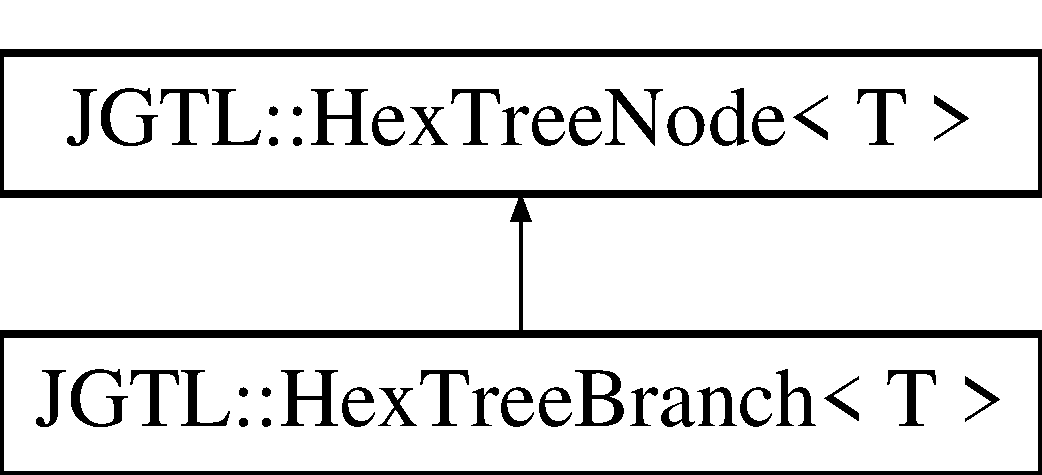
\includegraphics[height=2cm]{class_j_g_t_l_1_1_hex_tree_branch}
\end{center}
\end{figure}
\subsection*{Public Member Functions}
\begin{CompactItemize}
\item 
\hyperlink{class_j_g_t_l_1_1_hex_tree_branch_d7db0d8efdf004a111fc3e690e4382f5}{Hex\-Tree\-Branch} (pool$<$$>$ \&branch\-Pool, pool$<$$>$ \&stub\-Pool, const T \&value)
\item 
virtual \hyperlink{class_j_g_t_l_1_1_hex_tree_branch_72074225e2a22d7bf9642f47d67d8b05}{$\sim$Hex\-Tree\-Branch} ()
\item 
virtual void \hyperlink{class_j_g_t_l_1_1_hex_tree_branch_d89e805f2da424578087d92b0be7e35e}{destroy} (pool$<$$>$ \&branch\-Pool, pool$<$$>$ \&stub\-Pool)
\item 
int \hyperlink{class_j_g_t_l_1_1_hex_tree_branch_675bb8015ef743e126b2b5a8986195e5}{get\-Child\-Index} (const \hyperlink{class_j_g_t_l_1_1_vector4}{Vector4}$<$ int $>$ \&location, const \hyperlink{class_j_g_t_l_1_1_vector4}{Vector4}$<$ int $>$ \&center, const \hyperlink{class_j_g_t_l_1_1_vector4}{Vector4}$<$ int $>$ \&top\-Left\-Vector4, \hyperlink{class_j_g_t_l_1_1_vector4}{Vector4}$<$ int $>$ \&new\-Top\-Left\-Vector4) const 
\item 
virtual T \hyperlink{class_j_g_t_l_1_1_hex_tree_branch_e5124a6441d3e3d3c21f0d20124a3599}{get\-Value} (\hyperlink{class_j_g_t_l_1_1_vector4}{Vector4}$<$ int $>$ top\-Left\-Vector4, int size, const \hyperlink{class_j_g_t_l_1_1_vector4}{Vector4}$<$ int $>$ \&location) const 
\item 
virtual T \hyperlink{class_j_g_t_l_1_1_hex_tree_branch_25a53141349844dc869458f30db6f2a7}{get\-Value} () const
\item 
void \hyperlink{class_j_g_t_l_1_1_hex_tree_branch_2c1642e6125754f5ed1100d2422a7260}{set\-All} (pool$<$$>$ \&branch\-Pool, pool$<$$>$ \&stub\-Pool, T \&value)
\item 
virtual bool \hyperlink{class_j_g_t_l_1_1_hex_tree_branch_26769f998116310e9c17a03ee53f256c}{set\-Value} (pool$<$$>$ \&branch\-Pool, pool$<$$>$ \&stub\-Pool, \hyperlink{class_j_g_t_l_1_1_vector4}{Vector4}$<$ int $>$ top\-Left\-Vector4, int size, const \hyperlink{class_j_g_t_l_1_1_vector4}{Vector4}$<$ int $>$ \&location, const T \&value)
\item 
virtual void \hyperlink{class_j_g_t_l_1_1_hex_tree_branch_b9ca243a3f04629750ee65544b14e548}{display} (int level) const
\item 
virtual int \hyperlink{class_j_g_t_l_1_1_hex_tree_branch_84bea1c135b12ec017dfa3c701d0f9c9}{get\-Mem\-Usage} () const
\end{CompactItemize}
\subsection*{Private Attributes}
\begin{CompactItemize}
\item 
\hyperlink{class_j_g_t_l_1_1_hex_tree_node}{Hex\-Tree\-Node}$<$ T $>$ $\ast$ \hyperlink{class_j_g_t_l_1_1_hex_tree_branch_9917ee19fc32f342d487cb9d887887da}{children} \mbox{[}16\mbox{]}
\end{CompactItemize}
\subsubsection*{template$<$class T$>$ class JGTL::Hex\-Tree\-Branch$<$ T $>$}



\subsection{Constructor \& Destructor Documentation}
\hypertarget{class_j_g_t_l_1_1_hex_tree_branch_d7db0d8efdf004a111fc3e690e4382f5}{
\index{JGTL::HexTreeBranch@{JGTL::Hex\-Tree\-Branch}!HexTreeBranch@{HexTreeBranch}}
\index{HexTreeBranch@{HexTreeBranch}!JGTL::HexTreeBranch@{JGTL::Hex\-Tree\-Branch}}
\subsubsection[HexTreeBranch]{\setlength{\rightskip}{0pt plus 5cm}template$<$class T$>$ \hyperlink{class_j_g_t_l_1_1_hex_tree_branch}{JGTL::Hex\-Tree\-Branch}$<$ T $>$::\hyperlink{class_j_g_t_l_1_1_hex_tree_branch}{Hex\-Tree\-Branch} (pool$<$$>$ \& {\em branch\-Pool}, pool$<$$>$ \& {\em stub\-Pool}, const T \& {\em value})\hspace{0.3cm}{\tt  \mbox{[}inline\mbox{]}}}}
\label{class_j_g_t_l_1_1_hex_tree_branch_d7db0d8efdf004a111fc3e690e4382f5}


\hypertarget{class_j_g_t_l_1_1_hex_tree_branch_72074225e2a22d7bf9642f47d67d8b05}{
\index{JGTL::HexTreeBranch@{JGTL::Hex\-Tree\-Branch}!~HexTreeBranch@{$\sim$HexTreeBranch}}
\index{~HexTreeBranch@{$\sim$HexTreeBranch}!JGTL::HexTreeBranch@{JGTL::Hex\-Tree\-Branch}}
\subsubsection[$\sim$HexTreeBranch]{\setlength{\rightskip}{0pt plus 5cm}template$<$class T$>$ virtual \hyperlink{class_j_g_t_l_1_1_hex_tree_branch}{JGTL::Hex\-Tree\-Branch}$<$ T $>$::$\sim$\hyperlink{class_j_g_t_l_1_1_hex_tree_branch}{Hex\-Tree\-Branch} ()\hspace{0.3cm}{\tt  \mbox{[}inline, virtual\mbox{]}}}}
\label{class_j_g_t_l_1_1_hex_tree_branch_72074225e2a22d7bf9642f47d67d8b05}




\subsection{Member Function Documentation}
\hypertarget{class_j_g_t_l_1_1_hex_tree_branch_d89e805f2da424578087d92b0be7e35e}{
\index{JGTL::HexTreeBranch@{JGTL::Hex\-Tree\-Branch}!destroy@{destroy}}
\index{destroy@{destroy}!JGTL::HexTreeBranch@{JGTL::Hex\-Tree\-Branch}}
\subsubsection[destroy]{\setlength{\rightskip}{0pt plus 5cm}template$<$class T$>$ virtual void \hyperlink{class_j_g_t_l_1_1_hex_tree_branch}{JGTL::Hex\-Tree\-Branch}$<$ T $>$::destroy (pool$<$$>$ \& {\em branch\-Pool}, pool$<$$>$ \& {\em stub\-Pool})\hspace{0.3cm}{\tt  \mbox{[}inline, virtual\mbox{]}}}}
\label{class_j_g_t_l_1_1_hex_tree_branch_d89e805f2da424578087d92b0be7e35e}




Reimplemented from \hyperlink{class_j_g_t_l_1_1_hex_tree_node_f093e463c1b3247b587370802caa98f2}{JGTL::Hex\-Tree\-Node$<$ T $>$}.\hypertarget{class_j_g_t_l_1_1_hex_tree_branch_675bb8015ef743e126b2b5a8986195e5}{
\index{JGTL::HexTreeBranch@{JGTL::Hex\-Tree\-Branch}!getChildIndex@{getChildIndex}}
\index{getChildIndex@{getChildIndex}!JGTL::HexTreeBranch@{JGTL::Hex\-Tree\-Branch}}
\subsubsection[getChildIndex]{\setlength{\rightskip}{0pt plus 5cm}template$<$class T$>$ int \hyperlink{class_j_g_t_l_1_1_hex_tree_branch}{JGTL::Hex\-Tree\-Branch}$<$ T $>$::get\-Child\-Index (const \hyperlink{class_j_g_t_l_1_1_vector4}{Vector4}$<$ int $>$ \& {\em location}, const \hyperlink{class_j_g_t_l_1_1_vector4}{Vector4}$<$ int $>$ \& {\em center}, const \hyperlink{class_j_g_t_l_1_1_vector4}{Vector4}$<$ int $>$ \& {\em top\-Left\-Vector4}, \hyperlink{class_j_g_t_l_1_1_vector4}{Vector4}$<$ int $>$ \& {\em new\-Top\-Left\-Vector4}) const\hspace{0.3cm}{\tt  \mbox{[}inline\mbox{]}}}}
\label{class_j_g_t_l_1_1_hex_tree_branch_675bb8015ef743e126b2b5a8986195e5}


\hypertarget{class_j_g_t_l_1_1_hex_tree_branch_e5124a6441d3e3d3c21f0d20124a3599}{
\index{JGTL::HexTreeBranch@{JGTL::Hex\-Tree\-Branch}!getValue@{getValue}}
\index{getValue@{getValue}!JGTL::HexTreeBranch@{JGTL::Hex\-Tree\-Branch}}
\subsubsection[getValue]{\setlength{\rightskip}{0pt plus 5cm}template$<$class T$>$ virtual T \hyperlink{class_j_g_t_l_1_1_hex_tree_branch}{JGTL::Hex\-Tree\-Branch}$<$ T $>$::get\-Value (\hyperlink{class_j_g_t_l_1_1_vector4}{Vector4}$<$ int $>$ {\em top\-Left\-Vector4}, int {\em size}, const \hyperlink{class_j_g_t_l_1_1_vector4}{Vector4}$<$ int $>$ \& {\em location}) const\hspace{0.3cm}{\tt  \mbox{[}inline, virtual\mbox{]}}}}
\label{class_j_g_t_l_1_1_hex_tree_branch_e5124a6441d3e3d3c21f0d20124a3599}




Implements \hyperlink{class_j_g_t_l_1_1_hex_tree_node_64532266729bda54b7473acde6714604}{JGTL::Hex\-Tree\-Node$<$ T $>$}.\hypertarget{class_j_g_t_l_1_1_hex_tree_branch_25a53141349844dc869458f30db6f2a7}{
\index{JGTL::HexTreeBranch@{JGTL::Hex\-Tree\-Branch}!getValue@{getValue}}
\index{getValue@{getValue}!JGTL::HexTreeBranch@{JGTL::Hex\-Tree\-Branch}}
\subsubsection[getValue]{\setlength{\rightskip}{0pt plus 5cm}template$<$class T$>$ virtual T \hyperlink{class_j_g_t_l_1_1_hex_tree_branch}{JGTL::Hex\-Tree\-Branch}$<$ T $>$::get\-Value () const\hspace{0.3cm}{\tt  \mbox{[}inline, virtual\mbox{]}}}}
\label{class_j_g_t_l_1_1_hex_tree_branch_25a53141349844dc869458f30db6f2a7}




Implements \hyperlink{class_j_g_t_l_1_1_hex_tree_node_81dc320d9ae3cce6b5043696fa70a36d}{JGTL::Hex\-Tree\-Node$<$ T $>$}.\hypertarget{class_j_g_t_l_1_1_hex_tree_branch_2c1642e6125754f5ed1100d2422a7260}{
\index{JGTL::HexTreeBranch@{JGTL::Hex\-Tree\-Branch}!setAll@{setAll}}
\index{setAll@{setAll}!JGTL::HexTreeBranch@{JGTL::Hex\-Tree\-Branch}}
\subsubsection[setAll]{\setlength{\rightskip}{0pt plus 5cm}template$<$class T$>$ void \hyperlink{class_j_g_t_l_1_1_hex_tree_branch}{JGTL::Hex\-Tree\-Branch}$<$ T $>$::set\-All (pool$<$$>$ \& {\em branch\-Pool}, pool$<$$>$ \& {\em stub\-Pool}, T \& {\em value})\hspace{0.3cm}{\tt  \mbox{[}inline\mbox{]}}}}
\label{class_j_g_t_l_1_1_hex_tree_branch_2c1642e6125754f5ed1100d2422a7260}


\hypertarget{class_j_g_t_l_1_1_hex_tree_branch_26769f998116310e9c17a03ee53f256c}{
\index{JGTL::HexTreeBranch@{JGTL::Hex\-Tree\-Branch}!setValue@{setValue}}
\index{setValue@{setValue}!JGTL::HexTreeBranch@{JGTL::Hex\-Tree\-Branch}}
\subsubsection[setValue]{\setlength{\rightskip}{0pt plus 5cm}template$<$class T$>$ virtual bool \hyperlink{class_j_g_t_l_1_1_hex_tree_branch}{JGTL::Hex\-Tree\-Branch}$<$ T $>$::set\-Value (pool$<$$>$ \& {\em branch\-Pool}, pool$<$$>$ \& {\em stub\-Pool}, \hyperlink{class_j_g_t_l_1_1_vector4}{Vector4}$<$ int $>$ {\em top\-Left\-Vector4}, int {\em size}, const \hyperlink{class_j_g_t_l_1_1_vector4}{Vector4}$<$ int $>$ \& {\em location}, const T \& {\em value})\hspace{0.3cm}{\tt  \mbox{[}inline, virtual\mbox{]}}}}
\label{class_j_g_t_l_1_1_hex_tree_branch_26769f998116310e9c17a03ee53f256c}




Implements \hyperlink{class_j_g_t_l_1_1_hex_tree_node_a65570f2ecf17f3537a8a726795b4152}{JGTL::Hex\-Tree\-Node$<$ T $>$}.\hypertarget{class_j_g_t_l_1_1_hex_tree_branch_b9ca243a3f04629750ee65544b14e548}{
\index{JGTL::HexTreeBranch@{JGTL::Hex\-Tree\-Branch}!display@{display}}
\index{display@{display}!JGTL::HexTreeBranch@{JGTL::Hex\-Tree\-Branch}}
\subsubsection[display]{\setlength{\rightskip}{0pt plus 5cm}template$<$class T$>$ virtual void \hyperlink{class_j_g_t_l_1_1_hex_tree_branch}{JGTL::Hex\-Tree\-Branch}$<$ T $>$::display (int {\em level}) const\hspace{0.3cm}{\tt  \mbox{[}inline, virtual\mbox{]}}}}
\label{class_j_g_t_l_1_1_hex_tree_branch_b9ca243a3f04629750ee65544b14e548}




Implements \hyperlink{class_j_g_t_l_1_1_hex_tree_node_2031e26f8fbf11d061e51cdd0a6c27eb}{JGTL::Hex\-Tree\-Node$<$ T $>$}.\hypertarget{class_j_g_t_l_1_1_hex_tree_branch_84bea1c135b12ec017dfa3c701d0f9c9}{
\index{JGTL::HexTreeBranch@{JGTL::Hex\-Tree\-Branch}!getMemUsage@{getMemUsage}}
\index{getMemUsage@{getMemUsage}!JGTL::HexTreeBranch@{JGTL::Hex\-Tree\-Branch}}
\subsubsection[getMemUsage]{\setlength{\rightskip}{0pt plus 5cm}template$<$class T$>$ virtual int \hyperlink{class_j_g_t_l_1_1_hex_tree_branch}{JGTL::Hex\-Tree\-Branch}$<$ T $>$::get\-Mem\-Usage () const\hspace{0.3cm}{\tt  \mbox{[}inline, virtual\mbox{]}}}}
\label{class_j_g_t_l_1_1_hex_tree_branch_84bea1c135b12ec017dfa3c701d0f9c9}




Implements \hyperlink{class_j_g_t_l_1_1_hex_tree_node_9d71c1520ef1d80cf8ff292710e1994d}{JGTL::Hex\-Tree\-Node$<$ T $>$}.

\subsection{Member Data Documentation}
\hypertarget{class_j_g_t_l_1_1_hex_tree_branch_9917ee19fc32f342d487cb9d887887da}{
\index{JGTL::HexTreeBranch@{JGTL::Hex\-Tree\-Branch}!children@{children}}
\index{children@{children}!JGTL::HexTreeBranch@{JGTL::Hex\-Tree\-Branch}}
\subsubsection[children]{\setlength{\rightskip}{0pt plus 5cm}template$<$class T$>$ \hyperlink{class_j_g_t_l_1_1_hex_tree_node}{Hex\-Tree\-Node}$<$T$>$$\ast$ \hyperlink{class_j_g_t_l_1_1_hex_tree_branch}{JGTL::Hex\-Tree\-Branch}$<$ T $>$::\hyperlink{class_j_g_t_l_1_1_hex_tree_branch_9917ee19fc32f342d487cb9d887887da}{children}\mbox{[}16\mbox{]}\hspace{0.3cm}{\tt  \mbox{[}private\mbox{]}}}}
\label{class_j_g_t_l_1_1_hex_tree_branch_9917ee19fc32f342d487cb9d887887da}




The documentation for this class was generated from the following file:\begin{CompactItemize}
\item 
\hyperlink{_j_g_t_l___hex_tree_8h}{JGTL\_\-Hex\-Tree.h}\end{CompactItemize}

\hypertarget{class_j_g_t_l_1_1_hex_tree_node}{
\section{JGTL::Hex\-Tree\-Node$<$ T $>$ Class Template Reference}
\label{class_j_g_t_l_1_1_hex_tree_node}\index{JGTL::HexTreeNode@{JGTL::HexTreeNode}}
}
{\tt \#include $<$JGTL\_\-Hex\-Tree.h$>$}

Inheritance diagram for JGTL::Hex\-Tree\-Node$<$ T $>$::\begin{figure}[H]
\begin{center}
\leavevmode
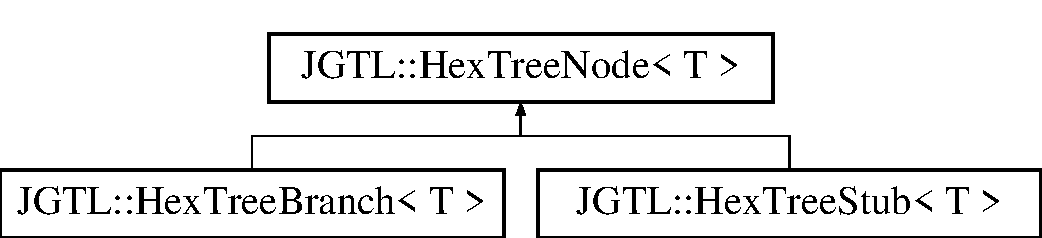
\includegraphics[height=2cm]{class_j_g_t_l_1_1_hex_tree_node}
\end{center}
\end{figure}
\subsection*{Public Member Functions}
\begin{CompactItemize}
\item 
\hyperlink{class_j_g_t_l_1_1_hex_tree_node_564ae11ac8eac7662e7fac5fc8c49f57}{Hex\-Tree\-Node} ()
\item 
virtual \hyperlink{class_j_g_t_l_1_1_hex_tree_node_274897364d0457a85e4efcc0ea9de0c4}{$\sim$Hex\-Tree\-Node} ()
\item 
virtual T \hyperlink{class_j_g_t_l_1_1_hex_tree_node_64532266729bda54b7473acde6714604}{get\-Value} (\hyperlink{class_j_g_t_l_1_1_vector4}{Vector4}$<$ int $>$ top\-Left\-Vector4, int size, const \hyperlink{class_j_g_t_l_1_1_vector4}{Vector4}$<$ int $>$ \&location) const =0
\item 
virtual T \hyperlink{class_j_g_t_l_1_1_hex_tree_node_81dc320d9ae3cce6b5043696fa70a36d}{get\-Value} () const=0
\item 
virtual bool \hyperlink{class_j_g_t_l_1_1_hex_tree_node_a65570f2ecf17f3537a8a726795b4152}{set\-Value} (pool$<$$>$ \&branch\-Pool, pool$<$$>$ \&stub\-Pool, \hyperlink{class_j_g_t_l_1_1_vector4}{Vector4}$<$ int $>$ top\-Left\-Vector4, int size, const \hyperlink{class_j_g_t_l_1_1_vector4}{Vector4}$<$ int $>$ \&location, const T \&value)=0
\item 
virtual bool \hyperlink{class_j_g_t_l_1_1_hex_tree_node_4d37c24c8c3830953d2a9f195d7d26b5}{is\-Stub} () const
\item 
virtual void \hyperlink{class_j_g_t_l_1_1_hex_tree_node_f093e463c1b3247b587370802caa98f2}{destroy} (pool$<$$>$ \&branch\-Pool, pool$<$$>$ \&stub\-Pool)
\item 
virtual void \hyperlink{class_j_g_t_l_1_1_hex_tree_node_2031e26f8fbf11d061e51cdd0a6c27eb}{display} (int level) const=0
\item 
virtual int \hyperlink{class_j_g_t_l_1_1_hex_tree_node_9d71c1520ef1d80cf8ff292710e1994d}{get\-Mem\-Usage} () const=0
\end{CompactItemize}
\subsubsection*{template$<$class T$>$ class JGTL::Hex\-Tree\-Node$<$ T $>$}



\subsection{Constructor \& Destructor Documentation}
\hypertarget{class_j_g_t_l_1_1_hex_tree_node_564ae11ac8eac7662e7fac5fc8c49f57}{
\index{JGTL::HexTreeNode@{JGTL::Hex\-Tree\-Node}!HexTreeNode@{HexTreeNode}}
\index{HexTreeNode@{HexTreeNode}!JGTL::HexTreeNode@{JGTL::Hex\-Tree\-Node}}
\subsubsection[HexTreeNode]{\setlength{\rightskip}{0pt plus 5cm}template$<$class T$>$ \hyperlink{class_j_g_t_l_1_1_hex_tree_node}{JGTL::Hex\-Tree\-Node}$<$ T $>$::\hyperlink{class_j_g_t_l_1_1_hex_tree_node}{Hex\-Tree\-Node} ()\hspace{0.3cm}{\tt  \mbox{[}inline\mbox{]}}}}
\label{class_j_g_t_l_1_1_hex_tree_node_564ae11ac8eac7662e7fac5fc8c49f57}


\hypertarget{class_j_g_t_l_1_1_hex_tree_node_274897364d0457a85e4efcc0ea9de0c4}{
\index{JGTL::HexTreeNode@{JGTL::Hex\-Tree\-Node}!~HexTreeNode@{$\sim$HexTreeNode}}
\index{~HexTreeNode@{$\sim$HexTreeNode}!JGTL::HexTreeNode@{JGTL::Hex\-Tree\-Node}}
\subsubsection[$\sim$HexTreeNode]{\setlength{\rightskip}{0pt plus 5cm}template$<$class T$>$ virtual \hyperlink{class_j_g_t_l_1_1_hex_tree_node}{JGTL::Hex\-Tree\-Node}$<$ T $>$::$\sim$\hyperlink{class_j_g_t_l_1_1_hex_tree_node}{Hex\-Tree\-Node} ()\hspace{0.3cm}{\tt  \mbox{[}inline, virtual\mbox{]}}}}
\label{class_j_g_t_l_1_1_hex_tree_node_274897364d0457a85e4efcc0ea9de0c4}




\subsection{Member Function Documentation}
\hypertarget{class_j_g_t_l_1_1_hex_tree_node_64532266729bda54b7473acde6714604}{
\index{JGTL::HexTreeNode@{JGTL::Hex\-Tree\-Node}!getValue@{getValue}}
\index{getValue@{getValue}!JGTL::HexTreeNode@{JGTL::Hex\-Tree\-Node}}
\subsubsection[getValue]{\setlength{\rightskip}{0pt plus 5cm}template$<$class T$>$ virtual T \hyperlink{class_j_g_t_l_1_1_hex_tree_node}{JGTL::Hex\-Tree\-Node}$<$ T $>$::get\-Value (\hyperlink{class_j_g_t_l_1_1_vector4}{Vector4}$<$ int $>$ {\em top\-Left\-Vector4}, int {\em size}, const \hyperlink{class_j_g_t_l_1_1_vector4}{Vector4}$<$ int $>$ \& {\em location}) const\hspace{0.3cm}{\tt  \mbox{[}pure virtual\mbox{]}}}}
\label{class_j_g_t_l_1_1_hex_tree_node_64532266729bda54b7473acde6714604}




Implemented in \hyperlink{class_j_g_t_l_1_1_hex_tree_stub_1ebd4ddd7a7ba70896837b289167f096}{JGTL::Hex\-Tree\-Stub$<$ T $>$}, and \hyperlink{class_j_g_t_l_1_1_hex_tree_branch_e5124a6441d3e3d3c21f0d20124a3599}{JGTL::Hex\-Tree\-Branch$<$ T $>$}.\hypertarget{class_j_g_t_l_1_1_hex_tree_node_81dc320d9ae3cce6b5043696fa70a36d}{
\index{JGTL::HexTreeNode@{JGTL::Hex\-Tree\-Node}!getValue@{getValue}}
\index{getValue@{getValue}!JGTL::HexTreeNode@{JGTL::Hex\-Tree\-Node}}
\subsubsection[getValue]{\setlength{\rightskip}{0pt plus 5cm}template$<$class T$>$ virtual T \hyperlink{class_j_g_t_l_1_1_hex_tree_node}{JGTL::Hex\-Tree\-Node}$<$ T $>$::get\-Value () const\hspace{0.3cm}{\tt  \mbox{[}pure virtual\mbox{]}}}}
\label{class_j_g_t_l_1_1_hex_tree_node_81dc320d9ae3cce6b5043696fa70a36d}




Implemented in \hyperlink{class_j_g_t_l_1_1_hex_tree_stub_7babf085fd8c43177bd5ad1e885b2ab5}{JGTL::Hex\-Tree\-Stub$<$ T $>$}, and \hyperlink{class_j_g_t_l_1_1_hex_tree_branch_25a53141349844dc869458f30db6f2a7}{JGTL::Hex\-Tree\-Branch$<$ T $>$}.\hypertarget{class_j_g_t_l_1_1_hex_tree_node_a65570f2ecf17f3537a8a726795b4152}{
\index{JGTL::HexTreeNode@{JGTL::Hex\-Tree\-Node}!setValue@{setValue}}
\index{setValue@{setValue}!JGTL::HexTreeNode@{JGTL::Hex\-Tree\-Node}}
\subsubsection[setValue]{\setlength{\rightskip}{0pt plus 5cm}template$<$class T$>$ virtual bool \hyperlink{class_j_g_t_l_1_1_hex_tree_node}{JGTL::Hex\-Tree\-Node}$<$ T $>$::set\-Value (pool$<$$>$ \& {\em branch\-Pool}, pool$<$$>$ \& {\em stub\-Pool}, \hyperlink{class_j_g_t_l_1_1_vector4}{Vector4}$<$ int $>$ {\em top\-Left\-Vector4}, int {\em size}, const \hyperlink{class_j_g_t_l_1_1_vector4}{Vector4}$<$ int $>$ \& {\em location}, const T \& {\em value})\hspace{0.3cm}{\tt  \mbox{[}pure virtual\mbox{]}}}}
\label{class_j_g_t_l_1_1_hex_tree_node_a65570f2ecf17f3537a8a726795b4152}




Implemented in \hyperlink{class_j_g_t_l_1_1_hex_tree_stub_0b7ce18da709ea3b283920b279b3a688}{JGTL::Hex\-Tree\-Stub$<$ T $>$}, and \hyperlink{class_j_g_t_l_1_1_hex_tree_branch_26769f998116310e9c17a03ee53f256c}{JGTL::Hex\-Tree\-Branch$<$ T $>$}.\hypertarget{class_j_g_t_l_1_1_hex_tree_node_4d37c24c8c3830953d2a9f195d7d26b5}{
\index{JGTL::HexTreeNode@{JGTL::Hex\-Tree\-Node}!isStub@{isStub}}
\index{isStub@{isStub}!JGTL::HexTreeNode@{JGTL::Hex\-Tree\-Node}}
\subsubsection[isStub]{\setlength{\rightskip}{0pt plus 5cm}template$<$class T$>$ virtual bool \hyperlink{class_j_g_t_l_1_1_hex_tree_node}{JGTL::Hex\-Tree\-Node}$<$ T $>$::is\-Stub () const\hspace{0.3cm}{\tt  \mbox{[}inline, virtual\mbox{]}}}}
\label{class_j_g_t_l_1_1_hex_tree_node_4d37c24c8c3830953d2a9f195d7d26b5}




Reimplemented in \hyperlink{class_j_g_t_l_1_1_hex_tree_stub_f2ed502b7b1c2090642589b8ce1d637f}{JGTL::Hex\-Tree\-Stub$<$ T $>$}.\hypertarget{class_j_g_t_l_1_1_hex_tree_node_f093e463c1b3247b587370802caa98f2}{
\index{JGTL::HexTreeNode@{JGTL::Hex\-Tree\-Node}!destroy@{destroy}}
\index{destroy@{destroy}!JGTL::HexTreeNode@{JGTL::Hex\-Tree\-Node}}
\subsubsection[destroy]{\setlength{\rightskip}{0pt plus 5cm}template$<$class T$>$ virtual void \hyperlink{class_j_g_t_l_1_1_hex_tree_node}{JGTL::Hex\-Tree\-Node}$<$ T $>$::destroy (pool$<$$>$ \& {\em branch\-Pool}, pool$<$$>$ \& {\em stub\-Pool})\hspace{0.3cm}{\tt  \mbox{[}inline, virtual\mbox{]}}}}
\label{class_j_g_t_l_1_1_hex_tree_node_f093e463c1b3247b587370802caa98f2}




Reimplemented in \hyperlink{class_j_g_t_l_1_1_hex_tree_branch_d89e805f2da424578087d92b0be7e35e}{JGTL::Hex\-Tree\-Branch$<$ T $>$}.\hypertarget{class_j_g_t_l_1_1_hex_tree_node_2031e26f8fbf11d061e51cdd0a6c27eb}{
\index{JGTL::HexTreeNode@{JGTL::Hex\-Tree\-Node}!display@{display}}
\index{display@{display}!JGTL::HexTreeNode@{JGTL::Hex\-Tree\-Node}}
\subsubsection[display]{\setlength{\rightskip}{0pt plus 5cm}template$<$class T$>$ virtual void \hyperlink{class_j_g_t_l_1_1_hex_tree_node}{JGTL::Hex\-Tree\-Node}$<$ T $>$::display (int {\em level}) const\hspace{0.3cm}{\tt  \mbox{[}pure virtual\mbox{]}}}}
\label{class_j_g_t_l_1_1_hex_tree_node_2031e26f8fbf11d061e51cdd0a6c27eb}




Implemented in \hyperlink{class_j_g_t_l_1_1_hex_tree_stub_aa4a8e4efcf4afe347e9e0bf7d5d32ba}{JGTL::Hex\-Tree\-Stub$<$ T $>$}, and \hyperlink{class_j_g_t_l_1_1_hex_tree_branch_b9ca243a3f04629750ee65544b14e548}{JGTL::Hex\-Tree\-Branch$<$ T $>$}.\hypertarget{class_j_g_t_l_1_1_hex_tree_node_9d71c1520ef1d80cf8ff292710e1994d}{
\index{JGTL::HexTreeNode@{JGTL::Hex\-Tree\-Node}!getMemUsage@{getMemUsage}}
\index{getMemUsage@{getMemUsage}!JGTL::HexTreeNode@{JGTL::Hex\-Tree\-Node}}
\subsubsection[getMemUsage]{\setlength{\rightskip}{0pt plus 5cm}template$<$class T$>$ virtual int \hyperlink{class_j_g_t_l_1_1_hex_tree_node}{JGTL::Hex\-Tree\-Node}$<$ T $>$::get\-Mem\-Usage () const\hspace{0.3cm}{\tt  \mbox{[}pure virtual\mbox{]}}}}
\label{class_j_g_t_l_1_1_hex_tree_node_9d71c1520ef1d80cf8ff292710e1994d}




Implemented in \hyperlink{class_j_g_t_l_1_1_hex_tree_stub_51ad9d73122cd1c356c1b8219941a6e7}{JGTL::Hex\-Tree\-Stub$<$ T $>$}, and \hyperlink{class_j_g_t_l_1_1_hex_tree_branch_84bea1c135b12ec017dfa3c701d0f9c9}{JGTL::Hex\-Tree\-Branch$<$ T $>$}.

The documentation for this class was generated from the following file:\begin{CompactItemize}
\item 
\hyperlink{_j_g_t_l___hex_tree_8h}{JGTL\_\-Hex\-Tree.h}\end{CompactItemize}

\hypertarget{class_j_g_t_l_1_1_hex_tree_stub}{
\section{JGTL::Hex\-Tree\-Stub$<$ T $>$ Class Template Reference}
\label{class_j_g_t_l_1_1_hex_tree_stub}\index{JGTL::HexTreeStub@{JGTL::HexTreeStub}}
}
{\tt \#include $<$JGTL\_\-Hex\-Tree.h$>$}

Inheritance diagram for JGTL::Hex\-Tree\-Stub$<$ T $>$::\begin{figure}[H]
\begin{center}
\leavevmode
\includegraphics[height=2cm]{class_j_g_t_l_1_1_hex_tree_stub}
\end{center}
\end{figure}
\subsection*{Public Member Functions}
\begin{CompactItemize}
\item 
\hyperlink{class_j_g_t_l_1_1_hex_tree_stub_b31acb7855ec45d8a98c96ab8793dda9}{Hex\-Tree\-Stub} (T \_\-value)
\item 
virtual \hyperlink{class_j_g_t_l_1_1_hex_tree_stub_5ea48e0459e81668d3a3457cb0037be9}{$\sim$Hex\-Tree\-Stub} ()
\item 
virtual T \hyperlink{class_j_g_t_l_1_1_hex_tree_stub_1ebd4ddd7a7ba70896837b289167f096}{get\-Value} (\hyperlink{class_j_g_t_l_1_1_vector4}{Vector4}$<$ int $>$ top\-Left\-Vector4, int size, const \hyperlink{class_j_g_t_l_1_1_vector4}{Vector4}$<$ int $>$ \&location) const 
\item 
virtual T \hyperlink{class_j_g_t_l_1_1_hex_tree_stub_7babf085fd8c43177bd5ad1e885b2ab5}{get\-Value} () const
\item 
virtual bool \hyperlink{class_j_g_t_l_1_1_hex_tree_stub_0b7ce18da709ea3b283920b279b3a688}{set\-Value} (pool$<$$>$ \&branch\-Pool, pool$<$$>$ \&stub\-Pool, \hyperlink{class_j_g_t_l_1_1_vector4}{Vector4}$<$ int $>$ top\-Left\-Vector4, int size, const \hyperlink{class_j_g_t_l_1_1_vector4}{Vector4}$<$ int $>$ \&location, const T \&\hyperlink{class_j_g_t_l_1_1_hex_tree_stub_36b120793bf8032e9047c22875890a72}{value})
\item 
virtual bool \hyperlink{class_j_g_t_l_1_1_hex_tree_stub_584fb62fed5dc1c98241660e81e4b875}{set\-Value} (const T \&\_\-value)
\item 
virtual bool \hyperlink{class_j_g_t_l_1_1_hex_tree_stub_f2ed502b7b1c2090642589b8ce1d637f}{is\-Stub} () const
\item 
virtual void \hyperlink{class_j_g_t_l_1_1_hex_tree_stub_aa4a8e4efcf4afe347e9e0bf7d5d32ba}{display} (int level) const
\item 
virtual int \hyperlink{class_j_g_t_l_1_1_hex_tree_stub_51ad9d73122cd1c356c1b8219941a6e7}{get\-Mem\-Usage} () const
\end{CompactItemize}
\subsection*{Protected Attributes}
\begin{CompactItemize}
\item 
T \hyperlink{class_j_g_t_l_1_1_hex_tree_stub_36b120793bf8032e9047c22875890a72}{value}
\end{CompactItemize}
\subsubsection*{template$<$class T$>$ class JGTL::Hex\-Tree\-Stub$<$ T $>$}



\subsection{Constructor \& Destructor Documentation}
\hypertarget{class_j_g_t_l_1_1_hex_tree_stub_b31acb7855ec45d8a98c96ab8793dda9}{
\index{JGTL::HexTreeStub@{JGTL::Hex\-Tree\-Stub}!HexTreeStub@{HexTreeStub}}
\index{HexTreeStub@{HexTreeStub}!JGTL::HexTreeStub@{JGTL::Hex\-Tree\-Stub}}
\subsubsection[HexTreeStub]{\setlength{\rightskip}{0pt plus 5cm}template$<$class T$>$ \hyperlink{class_j_g_t_l_1_1_hex_tree_stub}{JGTL::Hex\-Tree\-Stub}$<$ T $>$::\hyperlink{class_j_g_t_l_1_1_hex_tree_stub}{Hex\-Tree\-Stub} (T {\em \_\-value})\hspace{0.3cm}{\tt  \mbox{[}inline\mbox{]}}}}
\label{class_j_g_t_l_1_1_hex_tree_stub_b31acb7855ec45d8a98c96ab8793dda9}


\hypertarget{class_j_g_t_l_1_1_hex_tree_stub_5ea48e0459e81668d3a3457cb0037be9}{
\index{JGTL::HexTreeStub@{JGTL::Hex\-Tree\-Stub}!~HexTreeStub@{$\sim$HexTreeStub}}
\index{~HexTreeStub@{$\sim$HexTreeStub}!JGTL::HexTreeStub@{JGTL::Hex\-Tree\-Stub}}
\subsubsection[$\sim$HexTreeStub]{\setlength{\rightskip}{0pt plus 5cm}template$<$class T$>$ virtual \hyperlink{class_j_g_t_l_1_1_hex_tree_stub}{JGTL::Hex\-Tree\-Stub}$<$ T $>$::$\sim$\hyperlink{class_j_g_t_l_1_1_hex_tree_stub}{Hex\-Tree\-Stub} ()\hspace{0.3cm}{\tt  \mbox{[}inline, virtual\mbox{]}}}}
\label{class_j_g_t_l_1_1_hex_tree_stub_5ea48e0459e81668d3a3457cb0037be9}




\subsection{Member Function Documentation}
\hypertarget{class_j_g_t_l_1_1_hex_tree_stub_1ebd4ddd7a7ba70896837b289167f096}{
\index{JGTL::HexTreeStub@{JGTL::Hex\-Tree\-Stub}!getValue@{getValue}}
\index{getValue@{getValue}!JGTL::HexTreeStub@{JGTL::Hex\-Tree\-Stub}}
\subsubsection[getValue]{\setlength{\rightskip}{0pt plus 5cm}template$<$class T$>$ virtual T \hyperlink{class_j_g_t_l_1_1_hex_tree_stub}{JGTL::Hex\-Tree\-Stub}$<$ T $>$::get\-Value (\hyperlink{class_j_g_t_l_1_1_vector4}{Vector4}$<$ int $>$ {\em top\-Left\-Vector4}, int {\em size}, const \hyperlink{class_j_g_t_l_1_1_vector4}{Vector4}$<$ int $>$ \& {\em location}) const\hspace{0.3cm}{\tt  \mbox{[}inline, virtual\mbox{]}}}}
\label{class_j_g_t_l_1_1_hex_tree_stub_1ebd4ddd7a7ba70896837b289167f096}




Implements \hyperlink{class_j_g_t_l_1_1_hex_tree_node_64532266729bda54b7473acde6714604}{JGTL::Hex\-Tree\-Node$<$ T $>$}.\hypertarget{class_j_g_t_l_1_1_hex_tree_stub_7babf085fd8c43177bd5ad1e885b2ab5}{
\index{JGTL::HexTreeStub@{JGTL::Hex\-Tree\-Stub}!getValue@{getValue}}
\index{getValue@{getValue}!JGTL::HexTreeStub@{JGTL::Hex\-Tree\-Stub}}
\subsubsection[getValue]{\setlength{\rightskip}{0pt plus 5cm}template$<$class T$>$ virtual T \hyperlink{class_j_g_t_l_1_1_hex_tree_stub}{JGTL::Hex\-Tree\-Stub}$<$ T $>$::get\-Value () const\hspace{0.3cm}{\tt  \mbox{[}inline, virtual\mbox{]}}}}
\label{class_j_g_t_l_1_1_hex_tree_stub_7babf085fd8c43177bd5ad1e885b2ab5}




Implements \hyperlink{class_j_g_t_l_1_1_hex_tree_node_81dc320d9ae3cce6b5043696fa70a36d}{JGTL::Hex\-Tree\-Node$<$ T $>$}.\hypertarget{class_j_g_t_l_1_1_hex_tree_stub_0b7ce18da709ea3b283920b279b3a688}{
\index{JGTL::HexTreeStub@{JGTL::Hex\-Tree\-Stub}!setValue@{setValue}}
\index{setValue@{setValue}!JGTL::HexTreeStub@{JGTL::Hex\-Tree\-Stub}}
\subsubsection[setValue]{\setlength{\rightskip}{0pt plus 5cm}template$<$class T$>$ virtual bool \hyperlink{class_j_g_t_l_1_1_hex_tree_stub}{JGTL::Hex\-Tree\-Stub}$<$ T $>$::set\-Value (pool$<$$>$ \& {\em branch\-Pool}, pool$<$$>$ \& {\em stub\-Pool}, \hyperlink{class_j_g_t_l_1_1_vector4}{Vector4}$<$ int $>$ {\em top\-Left\-Vector4}, int {\em size}, const \hyperlink{class_j_g_t_l_1_1_vector4}{Vector4}$<$ int $>$ \& {\em location}, const T \& {\em value})\hspace{0.3cm}{\tt  \mbox{[}inline, virtual\mbox{]}}}}
\label{class_j_g_t_l_1_1_hex_tree_stub_0b7ce18da709ea3b283920b279b3a688}




Implements \hyperlink{class_j_g_t_l_1_1_hex_tree_node_a65570f2ecf17f3537a8a726795b4152}{JGTL::Hex\-Tree\-Node$<$ T $>$}.\hypertarget{class_j_g_t_l_1_1_hex_tree_stub_584fb62fed5dc1c98241660e81e4b875}{
\index{JGTL::HexTreeStub@{JGTL::Hex\-Tree\-Stub}!setValue@{setValue}}
\index{setValue@{setValue}!JGTL::HexTreeStub@{JGTL::Hex\-Tree\-Stub}}
\subsubsection[setValue]{\setlength{\rightskip}{0pt plus 5cm}template$<$class T$>$ virtual bool \hyperlink{class_j_g_t_l_1_1_hex_tree_stub}{JGTL::Hex\-Tree\-Stub}$<$ T $>$::set\-Value (const T \& {\em \_\-value})\hspace{0.3cm}{\tt  \mbox{[}inline, virtual\mbox{]}}}}
\label{class_j_g_t_l_1_1_hex_tree_stub_584fb62fed5dc1c98241660e81e4b875}


\hypertarget{class_j_g_t_l_1_1_hex_tree_stub_f2ed502b7b1c2090642589b8ce1d637f}{
\index{JGTL::HexTreeStub@{JGTL::Hex\-Tree\-Stub}!isStub@{isStub}}
\index{isStub@{isStub}!JGTL::HexTreeStub@{JGTL::Hex\-Tree\-Stub}}
\subsubsection[isStub]{\setlength{\rightskip}{0pt plus 5cm}template$<$class T$>$ virtual bool \hyperlink{class_j_g_t_l_1_1_hex_tree_stub}{JGTL::Hex\-Tree\-Stub}$<$ T $>$::is\-Stub () const\hspace{0.3cm}{\tt  \mbox{[}inline, virtual\mbox{]}}}}
\label{class_j_g_t_l_1_1_hex_tree_stub_f2ed502b7b1c2090642589b8ce1d637f}




Reimplemented from \hyperlink{class_j_g_t_l_1_1_hex_tree_node_4d37c24c8c3830953d2a9f195d7d26b5}{JGTL::Hex\-Tree\-Node$<$ T $>$}.\hypertarget{class_j_g_t_l_1_1_hex_tree_stub_aa4a8e4efcf4afe347e9e0bf7d5d32ba}{
\index{JGTL::HexTreeStub@{JGTL::Hex\-Tree\-Stub}!display@{display}}
\index{display@{display}!JGTL::HexTreeStub@{JGTL::Hex\-Tree\-Stub}}
\subsubsection[display]{\setlength{\rightskip}{0pt plus 5cm}template$<$class T$>$ virtual void \hyperlink{class_j_g_t_l_1_1_hex_tree_stub}{JGTL::Hex\-Tree\-Stub}$<$ T $>$::display (int {\em level}) const\hspace{0.3cm}{\tt  \mbox{[}inline, virtual\mbox{]}}}}
\label{class_j_g_t_l_1_1_hex_tree_stub_aa4a8e4efcf4afe347e9e0bf7d5d32ba}




Implements \hyperlink{class_j_g_t_l_1_1_hex_tree_node_2031e26f8fbf11d061e51cdd0a6c27eb}{JGTL::Hex\-Tree\-Node$<$ T $>$}.\hypertarget{class_j_g_t_l_1_1_hex_tree_stub_51ad9d73122cd1c356c1b8219941a6e7}{
\index{JGTL::HexTreeStub@{JGTL::Hex\-Tree\-Stub}!getMemUsage@{getMemUsage}}
\index{getMemUsage@{getMemUsage}!JGTL::HexTreeStub@{JGTL::Hex\-Tree\-Stub}}
\subsubsection[getMemUsage]{\setlength{\rightskip}{0pt plus 5cm}template$<$class T$>$ virtual int \hyperlink{class_j_g_t_l_1_1_hex_tree_stub}{JGTL::Hex\-Tree\-Stub}$<$ T $>$::get\-Mem\-Usage () const\hspace{0.3cm}{\tt  \mbox{[}inline, virtual\mbox{]}}}}
\label{class_j_g_t_l_1_1_hex_tree_stub_51ad9d73122cd1c356c1b8219941a6e7}




Implements \hyperlink{class_j_g_t_l_1_1_hex_tree_node_9d71c1520ef1d80cf8ff292710e1994d}{JGTL::Hex\-Tree\-Node$<$ T $>$}.

\subsection{Member Data Documentation}
\hypertarget{class_j_g_t_l_1_1_hex_tree_stub_36b120793bf8032e9047c22875890a72}{
\index{JGTL::HexTreeStub@{JGTL::Hex\-Tree\-Stub}!value@{value}}
\index{value@{value}!JGTL::HexTreeStub@{JGTL::Hex\-Tree\-Stub}}
\subsubsection[value]{\setlength{\rightskip}{0pt plus 5cm}template$<$class T$>$ T \hyperlink{class_j_g_t_l_1_1_hex_tree_stub}{JGTL::Hex\-Tree\-Stub}$<$ T $>$::\hyperlink{class_j_g_t_l_1_1_hex_tree_stub_36b120793bf8032e9047c22875890a72}{value}\hspace{0.3cm}{\tt  \mbox{[}protected\mbox{]}}}}
\label{class_j_g_t_l_1_1_hex_tree_stub_36b120793bf8032e9047c22875890a72}




The documentation for this class was generated from the following file:\begin{CompactItemize}
\item 
\hyperlink{_j_g_t_l___hex_tree_8h}{JGTL\_\-Hex\-Tree.h}\end{CompactItemize}

\hypertarget{struct_j_g_t_l_1_1_i_f}{
\section{JGTL::IF$<$ condition, Then, Else $>$ Struct Template Reference}
\label{struct_j_g_t_l_1_1_i_f}\index{JGTL::IF@{JGTL::IF}}
}
{\tt \#include $<$JGTL\_\-Integral\-Units.h$>$}

\subsection*{Public Types}
\begin{CompactItemize}
\item 
typedef Then \hyperlink{struct_j_g_t_l_1_1_i_f_e76ae6dfccd5d4c23b2d079f1a6a3b87}{RET}
\end{CompactItemize}
\subsubsection*{template$<$bool condition, class Then, class Else$>$ struct JGTL::IF$<$ condition, Then, Else $>$}



\subsection{Member Typedef Documentation}
\hypertarget{struct_j_g_t_l_1_1_i_f_e76ae6dfccd5d4c23b2d079f1a6a3b87}{
\index{JGTL::IF@{JGTL::IF}!RET@{RET}}
\index{RET@{RET}!JGTL::IF@{JGTL::IF}}
\subsubsection[RET]{\setlength{\rightskip}{0pt plus 5cm}template$<$bool condition, class Then, class Else$>$ typedef Then \hyperlink{struct_j_g_t_l_1_1_i_f}{JGTL::IF}$<$ condition, Then, Else $>$::\hyperlink{struct_j_g_t_l_1_1_i_f_e76ae6dfccd5d4c23b2d079f1a6a3b87}{RET}}}
\label{struct_j_g_t_l_1_1_i_f_e76ae6dfccd5d4c23b2d079f1a6a3b87}




The documentation for this struct was generated from the following file:\begin{CompactItemize}
\item 
\hyperlink{_j_g_t_l___integral_units_8h}{JGTL\_\-Integral\-Units.h}\end{CompactItemize}

\hypertarget{struct_j_g_t_l_1_1_i_f_3_01false_00_01_then_00_01_else_01_4}{
\section{JGTL::IF$<$ false, Then, Else $>$ Struct Template Reference}
\label{struct_j_g_t_l_1_1_i_f_3_01false_00_01_then_00_01_else_01_4}\index{JGTL::IF< false, Then, Else >@{JGTL::IF$<$ false, Then, Else $>$}}
}
{\tt \#include $<$JGTL\_\-Integral\-Units.h$>$}

\subsection*{Public Types}
\begin{CompactItemize}
\item 
typedef Else \hyperlink{struct_j_g_t_l_1_1_i_f_3_01false_00_01_then_00_01_else_01_4_471d3ff51488c1d43504d3eb98bd6f2b}{RET}
\end{CompactItemize}
\subsubsection*{template$<$class Then, class Else$>$ struct JGTL::IF$<$ false, Then, Else $>$}



\subsection{Member Typedef Documentation}
\hypertarget{struct_j_g_t_l_1_1_i_f_3_01false_00_01_then_00_01_else_01_4_471d3ff51488c1d43504d3eb98bd6f2b}{
\index{JGTL::IF< false, Then, Else >@{JGTL::IF$<$ false, Then, Else $>$}!RET@{RET}}
\index{RET@{RET}!JGTL::IF< false, Then, Else >@{JGTL::IF$<$ false, Then, Else $>$}}
\subsubsection[RET]{\setlength{\rightskip}{0pt plus 5cm}template$<$class Then, class Else$>$ typedef Else \hyperlink{struct_j_g_t_l_1_1_i_f}{JGTL::IF}$<$ false, Then, Else $>$::\hyperlink{struct_j_g_t_l_1_1_i_f_3_01false_00_01_then_00_01_else_01_4_471d3ff51488c1d43504d3eb98bd6f2b}{RET}}}
\label{struct_j_g_t_l_1_1_i_f_3_01false_00_01_then_00_01_else_01_4_471d3ff51488c1d43504d3eb98bd6f2b}




The documentation for this struct was generated from the following file:\begin{CompactItemize}
\item 
\hyperlink{_j_g_t_l___integral_units_8h}{JGTL\_\-Integral\-Units.h}\end{CompactItemize}

\hypertarget{class_j_g_t_l_1_1_index2}{
\section{JGTL::Index2 Class Reference}
\label{class_j_g_t_l_1_1_index2}\index{JGTL::Index2@{JGTL::Index2}}
}
{\tt \#include $<$JGTL\_\-Index2.h$>$}

\subsection*{Public Member Functions}
\begin{CompactItemize}
\item 
\hyperlink{class_j_g_t_l_1_1_index2_de79343237193d2af361ff7bb4c5c58b}{Index2} ()
\item 
\hyperlink{class_j_g_t_l_1_1_index2_7cf2a0b1b27b7f23e672dce3651977a4}{Index2} (int \_\-x, int \_\-y)
\item 
\hyperlink{class_j_g_t_l_1_1_index2_ba365e79cfd722dcb17518902ba3001c}{Index2} (std::string s)
\item 
Ogre::Vector2 \hyperlink{class_j_g_t_l_1_1_index2_e98b51555c8ece032c91aa828646ba15}{get\-Vector2} ()
\item 
std::string \hyperlink{class_j_g_t_l_1_1_index2_be2673713b217c79db1e93287a9aa2bb}{to\-String} ()
\item 
bool \hyperlink{class_j_g_t_l_1_1_index2_68ce5b51f0249e1ec5c9c06481ba8423}{operator==} (const \hyperlink{class_j_g_t_l_1_1_index2}{Index2} \&index)
\item 
bool \hyperlink{class_j_g_t_l_1_1_index2_e97a27cfa0c26e2dda554109f5770799}{operator!=} (const \hyperlink{class_j_g_t_l_1_1_index2}{Index2} \&index)
\end{CompactItemize}
\subsection*{Public Attributes}
\begin{CompactItemize}
\item 
int \hyperlink{class_j_g_t_l_1_1_index2_2890321cfbdc826c6e33f15e6a0a0f2f}{x}
\item 
int \hyperlink{class_j_g_t_l_1_1_index2_921a51f4736b4239217532c60a81fa31}{y}
\end{CompactItemize}


\subsection{Constructor \& Destructor Documentation}
\hypertarget{class_j_g_t_l_1_1_index2_de79343237193d2af361ff7bb4c5c58b}{
\index{JGTL::Index2@{JGTL::Index2}!Index2@{Index2}}
\index{Index2@{Index2}!JGTL::Index2@{JGTL::Index2}}
\subsubsection[Index2]{\setlength{\rightskip}{0pt plus 5cm}JGTL::Index2::Index2 ()}}
\label{class_j_g_t_l_1_1_index2_de79343237193d2af361ff7bb4c5c58b}


\hypertarget{class_j_g_t_l_1_1_index2_7cf2a0b1b27b7f23e672dce3651977a4}{
\index{JGTL::Index2@{JGTL::Index2}!Index2@{Index2}}
\index{Index2@{Index2}!JGTL::Index2@{JGTL::Index2}}
\subsubsection[Index2]{\setlength{\rightskip}{0pt plus 5cm}JGTL::Index2::Index2 (int {\em \_\-x}, int {\em \_\-y})}}
\label{class_j_g_t_l_1_1_index2_7cf2a0b1b27b7f23e672dce3651977a4}


\hypertarget{class_j_g_t_l_1_1_index2_ba365e79cfd722dcb17518902ba3001c}{
\index{JGTL::Index2@{JGTL::Index2}!Index2@{Index2}}
\index{Index2@{Index2}!JGTL::Index2@{JGTL::Index2}}
\subsubsection[Index2]{\setlength{\rightskip}{0pt plus 5cm}JGTL::Index2::Index2 (std::string {\em s})\hspace{0.3cm}{\tt  \mbox{[}inline\mbox{]}}}}
\label{class_j_g_t_l_1_1_index2_ba365e79cfd722dcb17518902ba3001c}




\subsection{Member Function Documentation}
\hypertarget{class_j_g_t_l_1_1_index2_e98b51555c8ece032c91aa828646ba15}{
\index{JGTL::Index2@{JGTL::Index2}!getVector2@{getVector2}}
\index{getVector2@{getVector2}!JGTL::Index2@{JGTL::Index2}}
\subsubsection[getVector2]{\setlength{\rightskip}{0pt plus 5cm}Ogre::Vector2 JGTL::Index2::get\-Vector2 ()\hspace{0.3cm}{\tt  \mbox{[}inline\mbox{]}}}}
\label{class_j_g_t_l_1_1_index2_e98b51555c8ece032c91aa828646ba15}


\hypertarget{class_j_g_t_l_1_1_index2_be2673713b217c79db1e93287a9aa2bb}{
\index{JGTL::Index2@{JGTL::Index2}!toString@{toString}}
\index{toString@{toString}!JGTL::Index2@{JGTL::Index2}}
\subsubsection[toString]{\setlength{\rightskip}{0pt plus 5cm}std::string JGTL::Index2::to\-String ()\hspace{0.3cm}{\tt  \mbox{[}inline\mbox{]}}}}
\label{class_j_g_t_l_1_1_index2_be2673713b217c79db1e93287a9aa2bb}


\hypertarget{class_j_g_t_l_1_1_index2_68ce5b51f0249e1ec5c9c06481ba8423}{
\index{JGTL::Index2@{JGTL::Index2}!operator==@{operator==}}
\index{operator==@{operator==}!JGTL::Index2@{JGTL::Index2}}
\subsubsection[operator==]{\setlength{\rightskip}{0pt plus 5cm}bool JGTL::Index2::operator== (const \hyperlink{class_j_g_t_l_1_1_index2}{Index2} \& {\em index})\hspace{0.3cm}{\tt  \mbox{[}inline\mbox{]}}}}
\label{class_j_g_t_l_1_1_index2_68ce5b51f0249e1ec5c9c06481ba8423}


\hypertarget{class_j_g_t_l_1_1_index2_e97a27cfa0c26e2dda554109f5770799}{
\index{JGTL::Index2@{JGTL::Index2}!operator"!=@{operator"!=}}
\index{operator"!=@{operator"!=}!JGTL::Index2@{JGTL::Index2}}
\subsubsection[operator"!=]{\setlength{\rightskip}{0pt plus 5cm}bool JGTL::Index2::operator!= (const \hyperlink{class_j_g_t_l_1_1_index2}{Index2} \& {\em index})\hspace{0.3cm}{\tt  \mbox{[}inline\mbox{]}}}}
\label{class_j_g_t_l_1_1_index2_e97a27cfa0c26e2dda554109f5770799}




\subsection{Member Data Documentation}
\hypertarget{class_j_g_t_l_1_1_index2_2890321cfbdc826c6e33f15e6a0a0f2f}{
\index{JGTL::Index2@{JGTL::Index2}!x@{x}}
\index{x@{x}!JGTL::Index2@{JGTL::Index2}}
\subsubsection[x]{\setlength{\rightskip}{0pt plus 5cm}int \hyperlink{class_j_g_t_l_1_1_index2_2890321cfbdc826c6e33f15e6a0a0f2f}{JGTL::Index2::x}}}
\label{class_j_g_t_l_1_1_index2_2890321cfbdc826c6e33f15e6a0a0f2f}


\hypertarget{class_j_g_t_l_1_1_index2_921a51f4736b4239217532c60a81fa31}{
\index{JGTL::Index2@{JGTL::Index2}!y@{y}}
\index{y@{y}!JGTL::Index2@{JGTL::Index2}}
\subsubsection[y]{\setlength{\rightskip}{0pt plus 5cm}int \hyperlink{class_j_g_t_l_1_1_index2_921a51f4736b4239217532c60a81fa31}{JGTL::Index2::y}}}
\label{class_j_g_t_l_1_1_index2_921a51f4736b4239217532c60a81fa31}




The documentation for this class was generated from the following file:\begin{CompactItemize}
\item 
\hyperlink{_j_g_t_l___index2_8h}{JGTL\_\-Index2.h}\end{CompactItemize}

\hypertarget{class_j_g_t_l_1_1_index3}{
\section{JGTL::Index3 Class Reference}
\label{class_j_g_t_l_1_1_index3}\index{JGTL::Index3@{JGTL::Index3}}
}
{\tt \#include $<$JGTL\_\-Index3.h$>$}

\subsection*{Public Member Functions}
\begin{CompactItemize}
\item 
\hyperlink{class_j_g_t_l_1_1_index3_f0f6a8a45c6d654d5a1849e2150460b3}{Index3} ()
\item 
\hyperlink{class_j_g_t_l_1_1_index3_31318bf64f28cdf0b0bd8aaf88dd6c80}{Index3} (int \_\-x, int \_\-y, int \_\-z)
\item 
\hyperlink{class_j_g_t_l_1_1_index3_57c5d0432d9042ef9c1c20eaff615ec7}{Index3} (std::string s)
\item 
bool \hyperlink{class_j_g_t_l_1_1_index3_28b74fda507cd39db2cb49bd7a9eda11}{operator$<$} (const \hyperlink{class_j_g_t_l_1_1_index3}{Index3} \&index) const 
\item 
bool \hyperlink{class_j_g_t_l_1_1_index3_e366c587a926599d5976c3ade146109a}{operator==} (const \hyperlink{class_j_g_t_l_1_1_index3}{Index3} \&index) const 
\item 
bool \hyperlink{class_j_g_t_l_1_1_index3_85560dbad6aa0d284112b99a59e58fb4}{operator!=} (const \hyperlink{class_j_g_t_l_1_1_index3}{Index3} \&index) const 
\item 
\hyperlink{class_j_g_t_l_1_1_index3}{Index3} \hyperlink{class_j_g_t_l_1_1_index3_095316d8fa8a9df4f70882eacbf2d98f}{operator $\ast$} (const \hyperlink{class_j_g_t_l_1_1_index3}{Index3} \&index) const 
\item 
template$<$class TT$>$ \hyperlink{class_j_g_t_l_1_1_index3}{Index3} \hyperlink{class_j_g_t_l_1_1_index3_68651bf3c423c5404e8dee156b5ad209}{operator $\ast$} (TT i) const 
\item 
\hyperlink{class_j_g_t_l_1_1_index3}{Index3} \hyperlink{class_j_g_t_l_1_1_index3_9ed9d700039569d2a90bb9d3274c4ddf}{operator/} (int i) const 
\item 
\hyperlink{class_j_g_t_l_1_1_index3}{Index3} \hyperlink{class_j_g_t_l_1_1_index3_acda81612eb294b96943b7693526f6dc}{operator-} (const \hyperlink{class_j_g_t_l_1_1_index3}{Index3} \&index) const 
\item 
void \hyperlink{class_j_g_t_l_1_1_index3_c204d4d42938bd7fc41c06041ad17661}{operator-=} (const \hyperlink{class_j_g_t_l_1_1_index3}{Index3} \&index)
\item 
\hyperlink{class_j_g_t_l_1_1_index3}{Index3} \hyperlink{class_j_g_t_l_1_1_index3_dc6ba4abf1475cdb42b5ea1fd5157414}{operator+} (const \hyperlink{class_j_g_t_l_1_1_index3}{Index3} \&index) const 
\item 
void \hyperlink{class_j_g_t_l_1_1_index3_28b8a687460de3b981aa58e2793459e6}{operator+=} (const \hyperlink{class_j_g_t_l_1_1_index3}{Index3} \&index)
\item 
double \hyperlink{class_j_g_t_l_1_1_index3_68ee3c05f26c463c7d936b94004ae097}{magnitude} () const
\item 
int \hyperlink{class_j_g_t_l_1_1_index3_c6cd24ce82dfa087a968646a9aa3fc58}{magnitude\-Squared} () const
\item 
int \hyperlink{class_j_g_t_l_1_1_index3_382f9ffa86227b2d180ea50ed3a9ddff}{distance\-Squared} (const \hyperlink{class_j_g_t_l_1_1_index3}{Index3} \&other) const 
\item 
int \hyperlink{class_j_g_t_l_1_1_index3_429d6d9c51948aec9bff8ae4e5df2b43}{distance\-Squared} (int \_\-x, int \_\-y, int \_\-z) const 
\item 
int \hyperlink{class_j_g_t_l_1_1_index3_acc8cad7f6ec9534c32c4a224c3b3670}{chess\-Distance} (const \hyperlink{class_j_g_t_l_1_1_index3}{Index3} \&other) const 
\item 
int \hyperlink{class_j_g_t_l_1_1_index3_97c6ed2e02b405f2e7c02208a54367c9}{manhat\-Distance} (const \hyperlink{class_j_g_t_l_1_1_index3}{Index3} \&other) const 
\end{CompactItemize}
\subsection*{Public Attributes}
\begin{CompactItemize}
\item 
int \hyperlink{class_j_g_t_l_1_1_index3_01306b4a1effbab2bf1358adb85ef7a1}{x}
\item 
int \hyperlink{class_j_g_t_l_1_1_index3_5723b9b685b7aaf559464973d1338e23}{y}
\item 
int \hyperlink{class_j_g_t_l_1_1_index3_bb74df1f3af23cf67605a319e27a0e55}{z}
\end{CompactItemize}


\subsection{Constructor \& Destructor Documentation}
\hypertarget{class_j_g_t_l_1_1_index3_f0f6a8a45c6d654d5a1849e2150460b3}{
\index{JGTL::Index3@{JGTL::Index3}!Index3@{Index3}}
\index{Index3@{Index3}!JGTL::Index3@{JGTL::Index3}}
\subsubsection[Index3]{\setlength{\rightskip}{0pt plus 5cm}JGTL::Index3::Index3 ()\hspace{0.3cm}{\tt  \mbox{[}inline\mbox{]}}}}
\label{class_j_g_t_l_1_1_index3_f0f6a8a45c6d654d5a1849e2150460b3}


\hypertarget{class_j_g_t_l_1_1_index3_31318bf64f28cdf0b0bd8aaf88dd6c80}{
\index{JGTL::Index3@{JGTL::Index3}!Index3@{Index3}}
\index{Index3@{Index3}!JGTL::Index3@{JGTL::Index3}}
\subsubsection[Index3]{\setlength{\rightskip}{0pt plus 5cm}JGTL::Index3::Index3 (int {\em \_\-x}, int {\em \_\-y}, int {\em \_\-z})\hspace{0.3cm}{\tt  \mbox{[}inline\mbox{]}}}}
\label{class_j_g_t_l_1_1_index3_31318bf64f28cdf0b0bd8aaf88dd6c80}


\hypertarget{class_j_g_t_l_1_1_index3_57c5d0432d9042ef9c1c20eaff615ec7}{
\index{JGTL::Index3@{JGTL::Index3}!Index3@{Index3}}
\index{Index3@{Index3}!JGTL::Index3@{JGTL::Index3}}
\subsubsection[Index3]{\setlength{\rightskip}{0pt plus 5cm}JGTL::Index3::Index3 (std::string {\em s})\hspace{0.3cm}{\tt  \mbox{[}inline\mbox{]}}}}
\label{class_j_g_t_l_1_1_index3_57c5d0432d9042ef9c1c20eaff615ec7}




\subsection{Member Function Documentation}
\hypertarget{class_j_g_t_l_1_1_index3_28b74fda507cd39db2cb49bd7a9eda11}{
\index{JGTL::Index3@{JGTL::Index3}!operator<@{operator$<$}}
\index{operator<@{operator$<$}!JGTL::Index3@{JGTL::Index3}}
\subsubsection[operator$<$]{\setlength{\rightskip}{0pt plus 5cm}bool JGTL::Index3::operator$<$ (const \hyperlink{class_j_g_t_l_1_1_index3}{Index3} \& {\em index}) const\hspace{0.3cm}{\tt  \mbox{[}inline\mbox{]}}}}
\label{class_j_g_t_l_1_1_index3_28b74fda507cd39db2cb49bd7a9eda11}


\hypertarget{class_j_g_t_l_1_1_index3_e366c587a926599d5976c3ade146109a}{
\index{JGTL::Index3@{JGTL::Index3}!operator==@{operator==}}
\index{operator==@{operator==}!JGTL::Index3@{JGTL::Index3}}
\subsubsection[operator==]{\setlength{\rightskip}{0pt plus 5cm}bool JGTL::Index3::operator== (const \hyperlink{class_j_g_t_l_1_1_index3}{Index3} \& {\em index}) const\hspace{0.3cm}{\tt  \mbox{[}inline\mbox{]}}}}
\label{class_j_g_t_l_1_1_index3_e366c587a926599d5976c3ade146109a}


\hypertarget{class_j_g_t_l_1_1_index3_85560dbad6aa0d284112b99a59e58fb4}{
\index{JGTL::Index3@{JGTL::Index3}!operator"!=@{operator"!=}}
\index{operator"!=@{operator"!=}!JGTL::Index3@{JGTL::Index3}}
\subsubsection[operator"!=]{\setlength{\rightskip}{0pt plus 5cm}bool JGTL::Index3::operator!= (const \hyperlink{class_j_g_t_l_1_1_index3}{Index3} \& {\em index}) const\hspace{0.3cm}{\tt  \mbox{[}inline\mbox{]}}}}
\label{class_j_g_t_l_1_1_index3_85560dbad6aa0d284112b99a59e58fb4}


\hypertarget{class_j_g_t_l_1_1_index3_095316d8fa8a9df4f70882eacbf2d98f}{
\index{JGTL::Index3@{JGTL::Index3}!operator *@{operator $\ast$}}
\index{operator *@{operator $\ast$}!JGTL::Index3@{JGTL::Index3}}
\subsubsection[operator $\ast$]{\setlength{\rightskip}{0pt plus 5cm}\hyperlink{class_j_g_t_l_1_1_index3}{Index3} JGTL::Index3::operator $\ast$ (const \hyperlink{class_j_g_t_l_1_1_index3}{Index3} \& {\em index}) const\hspace{0.3cm}{\tt  \mbox{[}inline\mbox{]}}}}
\label{class_j_g_t_l_1_1_index3_095316d8fa8a9df4f70882eacbf2d98f}


\hypertarget{class_j_g_t_l_1_1_index3_68651bf3c423c5404e8dee156b5ad209}{
\index{JGTL::Index3@{JGTL::Index3}!operator *@{operator $\ast$}}
\index{operator *@{operator $\ast$}!JGTL::Index3@{JGTL::Index3}}
\subsubsection[operator $\ast$]{\setlength{\rightskip}{0pt plus 5cm}template$<$class TT$>$ \hyperlink{class_j_g_t_l_1_1_index3}{Index3} JGTL::Index3::operator $\ast$ (TT {\em i}) const\hspace{0.3cm}{\tt  \mbox{[}inline\mbox{]}}}}
\label{class_j_g_t_l_1_1_index3_68651bf3c423c5404e8dee156b5ad209}


\hypertarget{class_j_g_t_l_1_1_index3_9ed9d700039569d2a90bb9d3274c4ddf}{
\index{JGTL::Index3@{JGTL::Index3}!operator/@{operator/}}
\index{operator/@{operator/}!JGTL::Index3@{JGTL::Index3}}
\subsubsection[operator/]{\setlength{\rightskip}{0pt plus 5cm}\hyperlink{class_j_g_t_l_1_1_index3}{Index3} JGTL::Index3::operator/ (int {\em i}) const\hspace{0.3cm}{\tt  \mbox{[}inline\mbox{]}}}}
\label{class_j_g_t_l_1_1_index3_9ed9d700039569d2a90bb9d3274c4ddf}


\hypertarget{class_j_g_t_l_1_1_index3_acda81612eb294b96943b7693526f6dc}{
\index{JGTL::Index3@{JGTL::Index3}!operator-@{operator-}}
\index{operator-@{operator-}!JGTL::Index3@{JGTL::Index3}}
\subsubsection[operator-]{\setlength{\rightskip}{0pt plus 5cm}\hyperlink{class_j_g_t_l_1_1_index3}{Index3} JGTL::Index3::operator- (const \hyperlink{class_j_g_t_l_1_1_index3}{Index3} \& {\em index}) const\hspace{0.3cm}{\tt  \mbox{[}inline\mbox{]}}}}
\label{class_j_g_t_l_1_1_index3_acda81612eb294b96943b7693526f6dc}


\hypertarget{class_j_g_t_l_1_1_index3_c204d4d42938bd7fc41c06041ad17661}{
\index{JGTL::Index3@{JGTL::Index3}!operator-=@{operator-=}}
\index{operator-=@{operator-=}!JGTL::Index3@{JGTL::Index3}}
\subsubsection[operator-=]{\setlength{\rightskip}{0pt plus 5cm}void JGTL::Index3::operator-= (const \hyperlink{class_j_g_t_l_1_1_index3}{Index3} \& {\em index})\hspace{0.3cm}{\tt  \mbox{[}inline\mbox{]}}}}
\label{class_j_g_t_l_1_1_index3_c204d4d42938bd7fc41c06041ad17661}


\hypertarget{class_j_g_t_l_1_1_index3_dc6ba4abf1475cdb42b5ea1fd5157414}{
\index{JGTL::Index3@{JGTL::Index3}!operator+@{operator+}}
\index{operator+@{operator+}!JGTL::Index3@{JGTL::Index3}}
\subsubsection[operator+]{\setlength{\rightskip}{0pt plus 5cm}\hyperlink{class_j_g_t_l_1_1_index3}{Index3} JGTL::Index3::operator+ (const \hyperlink{class_j_g_t_l_1_1_index3}{Index3} \& {\em index}) const\hspace{0.3cm}{\tt  \mbox{[}inline\mbox{]}}}}
\label{class_j_g_t_l_1_1_index3_dc6ba4abf1475cdb42b5ea1fd5157414}


\hypertarget{class_j_g_t_l_1_1_index3_28b8a687460de3b981aa58e2793459e6}{
\index{JGTL::Index3@{JGTL::Index3}!operator+=@{operator+=}}
\index{operator+=@{operator+=}!JGTL::Index3@{JGTL::Index3}}
\subsubsection[operator+=]{\setlength{\rightskip}{0pt plus 5cm}void JGTL::Index3::operator+= (const \hyperlink{class_j_g_t_l_1_1_index3}{Index3} \& {\em index})\hspace{0.3cm}{\tt  \mbox{[}inline\mbox{]}}}}
\label{class_j_g_t_l_1_1_index3_28b8a687460de3b981aa58e2793459e6}


\hypertarget{class_j_g_t_l_1_1_index3_68ee3c05f26c463c7d936b94004ae097}{
\index{JGTL::Index3@{JGTL::Index3}!magnitude@{magnitude}}
\index{magnitude@{magnitude}!JGTL::Index3@{JGTL::Index3}}
\subsubsection[magnitude]{\setlength{\rightskip}{0pt plus 5cm}double JGTL::Index3::magnitude () const\hspace{0.3cm}{\tt  \mbox{[}inline\mbox{]}}}}
\label{class_j_g_t_l_1_1_index3_68ee3c05f26c463c7d936b94004ae097}


\hypertarget{class_j_g_t_l_1_1_index3_c6cd24ce82dfa087a968646a9aa3fc58}{
\index{JGTL::Index3@{JGTL::Index3}!magnitudeSquared@{magnitudeSquared}}
\index{magnitudeSquared@{magnitudeSquared}!JGTL::Index3@{JGTL::Index3}}
\subsubsection[magnitudeSquared]{\setlength{\rightskip}{0pt plus 5cm}int JGTL::Index3::magnitude\-Squared () const\hspace{0.3cm}{\tt  \mbox{[}inline\mbox{]}}}}
\label{class_j_g_t_l_1_1_index3_c6cd24ce82dfa087a968646a9aa3fc58}


\hypertarget{class_j_g_t_l_1_1_index3_382f9ffa86227b2d180ea50ed3a9ddff}{
\index{JGTL::Index3@{JGTL::Index3}!distanceSquared@{distanceSquared}}
\index{distanceSquared@{distanceSquared}!JGTL::Index3@{JGTL::Index3}}
\subsubsection[distanceSquared]{\setlength{\rightskip}{0pt plus 5cm}int JGTL::Index3::distance\-Squared (const \hyperlink{class_j_g_t_l_1_1_index3}{Index3} \& {\em other}) const\hspace{0.3cm}{\tt  \mbox{[}inline\mbox{]}}}}
\label{class_j_g_t_l_1_1_index3_382f9ffa86227b2d180ea50ed3a9ddff}


\hypertarget{class_j_g_t_l_1_1_index3_429d6d9c51948aec9bff8ae4e5df2b43}{
\index{JGTL::Index3@{JGTL::Index3}!distanceSquared@{distanceSquared}}
\index{distanceSquared@{distanceSquared}!JGTL::Index3@{JGTL::Index3}}
\subsubsection[distanceSquared]{\setlength{\rightskip}{0pt plus 5cm}int JGTL::Index3::distance\-Squared (int {\em \_\-x}, int {\em \_\-y}, int {\em \_\-z}) const\hspace{0.3cm}{\tt  \mbox{[}inline\mbox{]}}}}
\label{class_j_g_t_l_1_1_index3_429d6d9c51948aec9bff8ae4e5df2b43}


\hypertarget{class_j_g_t_l_1_1_index3_acc8cad7f6ec9534c32c4a224c3b3670}{
\index{JGTL::Index3@{JGTL::Index3}!chessDistance@{chessDistance}}
\index{chessDistance@{chessDistance}!JGTL::Index3@{JGTL::Index3}}
\subsubsection[chessDistance]{\setlength{\rightskip}{0pt plus 5cm}int JGTL::Index3::chess\-Distance (const \hyperlink{class_j_g_t_l_1_1_index3}{Index3} \& {\em other}) const\hspace{0.3cm}{\tt  \mbox{[}inline\mbox{]}}}}
\label{class_j_g_t_l_1_1_index3_acc8cad7f6ec9534c32c4a224c3b3670}


\hypertarget{class_j_g_t_l_1_1_index3_97c6ed2e02b405f2e7c02208a54367c9}{
\index{JGTL::Index3@{JGTL::Index3}!manhatDistance@{manhatDistance}}
\index{manhatDistance@{manhatDistance}!JGTL::Index3@{JGTL::Index3}}
\subsubsection[manhatDistance]{\setlength{\rightskip}{0pt plus 5cm}int JGTL::Index3::manhat\-Distance (const \hyperlink{class_j_g_t_l_1_1_index3}{Index3} \& {\em other}) const\hspace{0.3cm}{\tt  \mbox{[}inline\mbox{]}}}}
\label{class_j_g_t_l_1_1_index3_97c6ed2e02b405f2e7c02208a54367c9}




\subsection{Member Data Documentation}
\hypertarget{class_j_g_t_l_1_1_index3_01306b4a1effbab2bf1358adb85ef7a1}{
\index{JGTL::Index3@{JGTL::Index3}!x@{x}}
\index{x@{x}!JGTL::Index3@{JGTL::Index3}}
\subsubsection[x]{\setlength{\rightskip}{0pt plus 5cm}int \hyperlink{class_j_g_t_l_1_1_index3_01306b4a1effbab2bf1358adb85ef7a1}{JGTL::Index3::x}}}
\label{class_j_g_t_l_1_1_index3_01306b4a1effbab2bf1358adb85ef7a1}


\hypertarget{class_j_g_t_l_1_1_index3_5723b9b685b7aaf559464973d1338e23}{
\index{JGTL::Index3@{JGTL::Index3}!y@{y}}
\index{y@{y}!JGTL::Index3@{JGTL::Index3}}
\subsubsection[y]{\setlength{\rightskip}{0pt plus 5cm}int \hyperlink{class_j_g_t_l_1_1_index3_5723b9b685b7aaf559464973d1338e23}{JGTL::Index3::y}}}
\label{class_j_g_t_l_1_1_index3_5723b9b685b7aaf559464973d1338e23}


\hypertarget{class_j_g_t_l_1_1_index3_bb74df1f3af23cf67605a319e27a0e55}{
\index{JGTL::Index3@{JGTL::Index3}!z@{z}}
\index{z@{z}!JGTL::Index3@{JGTL::Index3}}
\subsubsection[z]{\setlength{\rightskip}{0pt plus 5cm}int \hyperlink{class_j_g_t_l_1_1_index3_bb74df1f3af23cf67605a319e27a0e55}{JGTL::Index3::z}}}
\label{class_j_g_t_l_1_1_index3_bb74df1f3af23cf67605a319e27a0e55}




The documentation for this class was generated from the following file:\begin{CompactItemize}
\item 
\hyperlink{_j_g_t_l___index3_8h}{JGTL\_\-Index3.h}\end{CompactItemize}

\hypertarget{class_j_g_t_l_1_1_integral_units}{
\section{JGTL::Integral\-Units$<$ Value\-Type, SCALE, USEGCD $>$ Class Template Reference}
\label{class_j_g_t_l_1_1_integral_units}\index{JGTL::IntegralUnits@{JGTL::IntegralUnits}}
}
{\tt \#include $<$JGTL\_\-Integral\-Units.h$>$}

\subsection*{Public Member Functions}
\begin{CompactItemize}
\item 
\hyperlink{class_j_g_t_l_1_1_integral_units_7a0b8ab1d60ee081001d9f60ca277ff0}{Integral\-Units} (Value\-Type \_\-value=0)
\item 
template$<$class Other\-Value\-Type, Other\-Value\-Type OTHERSCALE, bool OTHERUSEGCD$>$ \hyperlink{class_j_g_t_l_1_1_integral_units_281fe4bd63b000d4c79695bbf1296748}{Integral\-Units} (const \hyperlink{class_j_g_t_l_1_1_integral_units}{Integral\-Units}$<$ Other\-Value\-Type, OTHERSCALE, OTHERUSEGCD $>$ \&t)
\item 
template$<$class Other\-Value\-Type, Other\-Value\-Type OTHERSCALE, bool OTHERUSEGCD$>$ const \hyperlink{class_j_g_t_l_1_1_integral_units}{Integral\-Units} \& \hyperlink{class_j_g_t_l_1_1_integral_units_6aff5273f65110cf3bda1bea9d27c779}{operator=} (const \hyperlink{class_j_g_t_l_1_1_integral_units}{Integral\-Units}$<$ Other\-Value\-Type, OTHERSCALE, OTHERUSEGCD $>$ \&t)
\item 
template$<$class Other\-Value\-Type, Other\-Value\-Type OTHERSCALE, bool OTHERUSEGCD$>$ Value\-Type \hyperlink{class_j_g_t_l_1_1_integral_units_44144b6bf0109bf22d742c52fefaa63f}{change\-Scale} (const \hyperlink{class_j_g_t_l_1_1_integral_units}{Integral\-Units}$<$ Other\-Value\-Type, OTHERSCALE, OTHERUSEGCD $>$ \&t)
\item 
virtual \hyperlink{namespace_j_g_t_l_1924d6fd42e2d9661bc0b5a5063b99b3}{units\_\-internal\_\-ulong} \hyperlink{class_j_g_t_l_1_1_integral_units_c993e88b13af685bbd5a30975a0cfdc9}{get\-Scale} () const
\item 
void \hyperlink{class_j_g_t_l_1_1_integral_units_48ec23dc962dd95e11f6ff0b3ef76084}{set\-Value} (Value\-Type \_\-value)
\item 
Value\-Type \hyperlink{class_j_g_t_l_1_1_integral_units_38c178cd9a819a246614696fd8c9f982}{get\-Value} () const
\end{CompactItemize}
\subsection*{Protected Attributes}
\begin{CompactItemize}
\item 
Value\-Type \hyperlink{class_j_g_t_l_1_1_integral_units_dd460e258138ea7485333fda3cfd8cd1}{value}
\end{CompactItemize}
\subsubsection*{template$<$class Value\-Type, Value\-Type SCALE, bool USEGCD$>$ class JGTL::Integral\-Units$<$ Value\-Type, SCALE, USEGCD $>$}



\subsection{Constructor \& Destructor Documentation}
\hypertarget{class_j_g_t_l_1_1_integral_units_7a0b8ab1d60ee081001d9f60ca277ff0}{
\index{JGTL::IntegralUnits@{JGTL::Integral\-Units}!IntegralUnits@{IntegralUnits}}
\index{IntegralUnits@{IntegralUnits}!JGTL::IntegralUnits@{JGTL::Integral\-Units}}
\subsubsection[IntegralUnits]{\setlength{\rightskip}{0pt plus 5cm}template$<$class Value\-Type, Value\-Type SCALE, bool USEGCD$>$ \hyperlink{class_j_g_t_l_1_1_integral_units}{JGTL::Integral\-Units}$<$ Value\-Type, SCALE, USEGCD $>$::\hyperlink{class_j_g_t_l_1_1_integral_units}{Integral\-Units} (Value\-Type {\em \_\-value} = {\tt 0})\hspace{0.3cm}{\tt  \mbox{[}inline\mbox{]}}}}
\label{class_j_g_t_l_1_1_integral_units_7a0b8ab1d60ee081001d9f60ca277ff0}


\hypertarget{class_j_g_t_l_1_1_integral_units_281fe4bd63b000d4c79695bbf1296748}{
\index{JGTL::IntegralUnits@{JGTL::Integral\-Units}!IntegralUnits@{IntegralUnits}}
\index{IntegralUnits@{IntegralUnits}!JGTL::IntegralUnits@{JGTL::Integral\-Units}}
\subsubsection[IntegralUnits]{\setlength{\rightskip}{0pt plus 5cm}template$<$class Value\-Type, Value\-Type SCALE, bool USEGCD$>$ template$<$class Other\-Value\-Type, Other\-Value\-Type OTHERSCALE, bool OTHERUSEGCD$>$ \hyperlink{class_j_g_t_l_1_1_integral_units}{JGTL::Integral\-Units}$<$ Value\-Type, SCALE, USEGCD $>$::\hyperlink{class_j_g_t_l_1_1_integral_units}{Integral\-Units} (const \hyperlink{class_j_g_t_l_1_1_integral_units}{Integral\-Units}$<$ Other\-Value\-Type, OTHERSCALE, OTHERUSEGCD $>$ \& {\em t})\hspace{0.3cm}{\tt  \mbox{[}inline\mbox{]}}}}
\label{class_j_g_t_l_1_1_integral_units_281fe4bd63b000d4c79695bbf1296748}




\subsection{Member Function Documentation}
\hypertarget{class_j_g_t_l_1_1_integral_units_6aff5273f65110cf3bda1bea9d27c779}{
\index{JGTL::IntegralUnits@{JGTL::Integral\-Units}!operator=@{operator=}}
\index{operator=@{operator=}!JGTL::IntegralUnits@{JGTL::Integral\-Units}}
\subsubsection[operator=]{\setlength{\rightskip}{0pt plus 5cm}template$<$class Value\-Type, Value\-Type SCALE, bool USEGCD$>$ template$<$class Other\-Value\-Type, Other\-Value\-Type OTHERSCALE, bool OTHERUSEGCD$>$ const \hyperlink{class_j_g_t_l_1_1_integral_units}{Integral\-Units}\& \hyperlink{class_j_g_t_l_1_1_integral_units}{JGTL::Integral\-Units}$<$ Value\-Type, SCALE, USEGCD $>$::operator= (const \hyperlink{class_j_g_t_l_1_1_integral_units}{Integral\-Units}$<$ Other\-Value\-Type, OTHERSCALE, OTHERUSEGCD $>$ \& {\em t})\hspace{0.3cm}{\tt  \mbox{[}inline\mbox{]}}}}
\label{class_j_g_t_l_1_1_integral_units_6aff5273f65110cf3bda1bea9d27c779}


\hypertarget{class_j_g_t_l_1_1_integral_units_44144b6bf0109bf22d742c52fefaa63f}{
\index{JGTL::IntegralUnits@{JGTL::Integral\-Units}!changeScale@{changeScale}}
\index{changeScale@{changeScale}!JGTL::IntegralUnits@{JGTL::Integral\-Units}}
\subsubsection[changeScale]{\setlength{\rightskip}{0pt plus 5cm}template$<$class Value\-Type, Value\-Type SCALE, bool USEGCD$>$ template$<$class Other\-Value\-Type, Other\-Value\-Type OTHERSCALE, bool OTHERUSEGCD$>$ Value\-Type \hyperlink{class_j_g_t_l_1_1_integral_units}{JGTL::Integral\-Units}$<$ Value\-Type, SCALE, USEGCD $>$::change\-Scale (const \hyperlink{class_j_g_t_l_1_1_integral_units}{Integral\-Units}$<$ Other\-Value\-Type, OTHERSCALE, OTHERUSEGCD $>$ \& {\em t})\hspace{0.3cm}{\tt  \mbox{[}inline\mbox{]}}}}
\label{class_j_g_t_l_1_1_integral_units_44144b6bf0109bf22d742c52fefaa63f}


\hypertarget{class_j_g_t_l_1_1_integral_units_c993e88b13af685bbd5a30975a0cfdc9}{
\index{JGTL::IntegralUnits@{JGTL::Integral\-Units}!getScale@{getScale}}
\index{getScale@{getScale}!JGTL::IntegralUnits@{JGTL::Integral\-Units}}
\subsubsection[getScale]{\setlength{\rightskip}{0pt plus 5cm}template$<$class Value\-Type, Value\-Type SCALE, bool USEGCD$>$ virtual \hyperlink{namespace_j_g_t_l_1924d6fd42e2d9661bc0b5a5063b99b3}{units\_\-internal\_\-ulong} \hyperlink{class_j_g_t_l_1_1_integral_units}{JGTL::Integral\-Units}$<$ Value\-Type, SCALE, USEGCD $>$::get\-Scale () const\hspace{0.3cm}{\tt  \mbox{[}inline, virtual\mbox{]}}}}
\label{class_j_g_t_l_1_1_integral_units_c993e88b13af685bbd5a30975a0cfdc9}


\hypertarget{class_j_g_t_l_1_1_integral_units_48ec23dc962dd95e11f6ff0b3ef76084}{
\index{JGTL::IntegralUnits@{JGTL::Integral\-Units}!setValue@{setValue}}
\index{setValue@{setValue}!JGTL::IntegralUnits@{JGTL::Integral\-Units}}
\subsubsection[setValue]{\setlength{\rightskip}{0pt plus 5cm}template$<$class Value\-Type, Value\-Type SCALE, bool USEGCD$>$ void \hyperlink{class_j_g_t_l_1_1_integral_units}{JGTL::Integral\-Units}$<$ Value\-Type, SCALE, USEGCD $>$::set\-Value (Value\-Type {\em \_\-value})\hspace{0.3cm}{\tt  \mbox{[}inline\mbox{]}}}}
\label{class_j_g_t_l_1_1_integral_units_48ec23dc962dd95e11f6ff0b3ef76084}


\hypertarget{class_j_g_t_l_1_1_integral_units_38c178cd9a819a246614696fd8c9f982}{
\index{JGTL::IntegralUnits@{JGTL::Integral\-Units}!getValue@{getValue}}
\index{getValue@{getValue}!JGTL::IntegralUnits@{JGTL::Integral\-Units}}
\subsubsection[getValue]{\setlength{\rightskip}{0pt plus 5cm}template$<$class Value\-Type, Value\-Type SCALE, bool USEGCD$>$ Value\-Type \hyperlink{class_j_g_t_l_1_1_integral_units}{JGTL::Integral\-Units}$<$ Value\-Type, SCALE, USEGCD $>$::get\-Value () const\hspace{0.3cm}{\tt  \mbox{[}inline\mbox{]}}}}
\label{class_j_g_t_l_1_1_integral_units_38c178cd9a819a246614696fd8c9f982}




\subsection{Member Data Documentation}
\hypertarget{class_j_g_t_l_1_1_integral_units_dd460e258138ea7485333fda3cfd8cd1}{
\index{JGTL::IntegralUnits@{JGTL::Integral\-Units}!value@{value}}
\index{value@{value}!JGTL::IntegralUnits@{JGTL::Integral\-Units}}
\subsubsection[value]{\setlength{\rightskip}{0pt plus 5cm}template$<$class Value\-Type, Value\-Type SCALE, bool USEGCD$>$ Value\-Type \hyperlink{class_j_g_t_l_1_1_integral_units}{JGTL::Integral\-Units}$<$ Value\-Type, SCALE, USEGCD $>$::\hyperlink{class_j_g_t_l_1_1_integral_units_dd460e258138ea7485333fda3cfd8cd1}{value}\hspace{0.3cm}{\tt  \mbox{[}protected\mbox{]}}}}
\label{class_j_g_t_l_1_1_integral_units_dd460e258138ea7485333fda3cfd8cd1}




The documentation for this class was generated from the following file:\begin{CompactItemize}
\item 
\hyperlink{_j_g_t_l___integral_units_8h}{JGTL\_\-Integral\-Units.h}\end{CompactItemize}

\hypertarget{struct_j_g_t_l_1_1_integral_units_g_c_d}{
\section{JGTL::Integral\-Units\-GCD$<$ i, j $>$ Struct Template Reference}
\label{struct_j_g_t_l_1_1_integral_units_g_c_d}\index{JGTL::IntegralUnitsGCD@{JGTL::IntegralUnitsGCD}}
}
{\tt \#include $<$JGTL\_\-Integral\-Units.h$>$}

\subsection*{Static Public Attributes}
\begin{CompactItemize}
\item 
static const \hyperlink{namespace_j_g_t_l_1924d6fd42e2d9661bc0b5a5063b99b3}{units\_\-internal\_\-ulong} \hyperlink{struct_j_g_t_l_1_1_integral_units_g_c_d_ac0b8330d1fad96221c65bace9f042b5}{VALUE}
\end{CompactItemize}
\subsubsection*{template$<$units\_\-internal\_\-ulong i, units\_\-internal\_\-ulong j$>$ struct JGTL::Integral\-Units\-GCD$<$ i, j $>$}



\subsection{Member Data Documentation}
\hypertarget{struct_j_g_t_l_1_1_integral_units_g_c_d_ac0b8330d1fad96221c65bace9f042b5}{
\index{JGTL::IntegralUnitsGCD@{JGTL::Integral\-Units\-GCD}!VALUE@{VALUE}}
\index{VALUE@{VALUE}!JGTL::IntegralUnitsGCD@{JGTL::Integral\-Units\-GCD}}
\subsubsection[VALUE]{\setlength{\rightskip}{0pt plus 5cm}template$<$units\_\-internal\_\-ulong i, units\_\-internal\_\-ulong j$>$ const \hyperlink{namespace_j_g_t_l_1924d6fd42e2d9661bc0b5a5063b99b3}{units\_\-internal\_\-ulong} \hyperlink{struct_j_g_t_l_1_1_integral_units_g_c_d}{JGTL::Integral\-Units\-GCD}$<$ i, j $>$::\hyperlink{struct_j_g_t_l_1_1_integral_units_g_c_d_ac0b8330d1fad96221c65bace9f042b5}{VALUE}\hspace{0.3cm}{\tt  \mbox{[}static\mbox{]}}}}
\label{struct_j_g_t_l_1_1_integral_units_g_c_d_ac0b8330d1fad96221c65bace9f042b5}


\textbf{Initial value:}

\begin{Code}\begin{verbatim} TYPEIF< 
                        units_internal_ulong,
                        STATIC_MOD<units_internal_ulong,i,j>::VALUE==0, 
                        (j), 
                        TYPEIF< 
                        units_internal_ulong,
                        STATIC_MOD<units_internal_ulong,j,STATIC_MOD<units_internal_ulong,i,j>::VALUE>::VALUE==0,
                        STATIC_MOD<units_internal_ulong,i,j>::VALUE,
                        IntegralUnitsGCD<
                        STATIC_MOD<units_internal_ulong,i,j>::VALUE,
                        STATIC_MOD<units_internal_ulong,j,STATIC_MOD<units_internal_ulong,i,j>::VALUE>::VALUE
                        >::VALUE
                        >::RESULT 
                >::RESULT
\end{verbatim}\end{Code}


The documentation for this struct was generated from the following file:\begin{CompactItemize}
\item 
\hyperlink{_j_g_t_l___integral_units_8h}{JGTL\_\-Integral\-Units.h}\end{CompactItemize}

\hypertarget{struct_j_g_t_l_1_1_integral_units_g_c_d_3_010_00_010_01_4}{
\section{JGTL::Integral\-Units\-GCD$<$ 0, 0 $>$ Struct Template Reference}
\label{struct_j_g_t_l_1_1_integral_units_g_c_d_3_010_00_010_01_4}\index{JGTL::IntegralUnitsGCD< 0, 0 >@{JGTL::IntegralUnitsGCD$<$ 0, 0 $>$}}
}
{\tt \#include $<$JGTL\_\-Integral\-Units.h$>$}

\subsection*{Static Public Attributes}
\begin{CompactItemize}
\item 
static const \hyperlink{namespace_j_g_t_l_1924d6fd42e2d9661bc0b5a5063b99b3}{units\_\-internal\_\-ulong} \hyperlink{struct_j_g_t_l_1_1_integral_units_g_c_d_3_010_00_010_01_4_bf43633dc7cfc1480ea337375ee1fea8}{VALUE} = 0
\end{CompactItemize}
\subsubsection*{template$<$$>$ struct JGTL::Integral\-Units\-GCD$<$ 0, 0 $>$}



\subsection{Member Data Documentation}
\hypertarget{struct_j_g_t_l_1_1_integral_units_g_c_d_3_010_00_010_01_4_bf43633dc7cfc1480ea337375ee1fea8}{
\index{JGTL::IntegralUnitsGCD< 0, 0 >@{JGTL::Integral\-Units\-GCD$<$ 0, 0 $>$}!VALUE@{VALUE}}
\index{VALUE@{VALUE}!JGTL::IntegralUnitsGCD< 0, 0 >@{JGTL::Integral\-Units\-GCD$<$ 0, 0 $>$}}
\subsubsection[VALUE]{\setlength{\rightskip}{0pt plus 5cm}const \hyperlink{namespace_j_g_t_l_1924d6fd42e2d9661bc0b5a5063b99b3}{units\_\-internal\_\-ulong} \hyperlink{struct_j_g_t_l_1_1_integral_units_g_c_d}{JGTL::Integral\-Units\-GCD}$<$ 0, 0 $>$::\hyperlink{struct_j_g_t_l_1_1_integral_units_g_c_d_3_010_00_010_01_4_bf43633dc7cfc1480ea337375ee1fea8}{VALUE} = 0\hspace{0.3cm}{\tt  \mbox{[}static\mbox{]}}}}
\label{struct_j_g_t_l_1_1_integral_units_g_c_d_3_010_00_010_01_4_bf43633dc7cfc1480ea337375ee1fea8}




The documentation for this struct was generated from the following file:\begin{CompactItemize}
\item 
\hyperlink{_j_g_t_l___integral_units_8h}{JGTL\_\-Integral\-Units.h}\end{CompactItemize}

\hypertarget{struct_j_g_t_l_1_1_integral_units_g_c_d_3_010_00_01j_01_4}{
\section{JGTL::Integral\-Units\-GCD$<$ 0, j $>$ Struct Template Reference}
\label{struct_j_g_t_l_1_1_integral_units_g_c_d_3_010_00_01j_01_4}\index{JGTL::IntegralUnitsGCD< 0, j >@{JGTL::IntegralUnitsGCD$<$ 0, j $>$}}
}
{\tt \#include $<$JGTL\_\-Integral\-Units.h$>$}

\subsection*{Static Public Attributes}
\begin{CompactItemize}
\item 
static const \hyperlink{namespace_j_g_t_l_1924d6fd42e2d9661bc0b5a5063b99b3}{units\_\-internal\_\-ulong} \hyperlink{struct_j_g_t_l_1_1_integral_units_g_c_d_3_010_00_01j_01_4_5d6ce78c33f337aa3767ae203c04d9e8}{VALUE} = 0
\end{CompactItemize}
\subsubsection*{template$<$units\_\-internal\_\-ulong j$>$ struct JGTL::Integral\-Units\-GCD$<$ 0, j $>$}



\subsection{Member Data Documentation}
\hypertarget{struct_j_g_t_l_1_1_integral_units_g_c_d_3_010_00_01j_01_4_5d6ce78c33f337aa3767ae203c04d9e8}{
\index{JGTL::IntegralUnitsGCD< 0, j >@{JGTL::Integral\-Units\-GCD$<$ 0, j $>$}!VALUE@{VALUE}}
\index{VALUE@{VALUE}!JGTL::IntegralUnitsGCD< 0, j >@{JGTL::Integral\-Units\-GCD$<$ 0, j $>$}}
\subsubsection[VALUE]{\setlength{\rightskip}{0pt plus 5cm}template$<$units\_\-internal\_\-ulong j$>$ const \hyperlink{namespace_j_g_t_l_1924d6fd42e2d9661bc0b5a5063b99b3}{units\_\-internal\_\-ulong} \hyperlink{struct_j_g_t_l_1_1_integral_units_g_c_d}{JGTL::Integral\-Units\-GCD}$<$ 0, j $>$::\hyperlink{struct_j_g_t_l_1_1_integral_units_g_c_d_3_010_00_01j_01_4_5d6ce78c33f337aa3767ae203c04d9e8}{VALUE} = 0\hspace{0.3cm}{\tt  \mbox{[}static\mbox{]}}}}
\label{struct_j_g_t_l_1_1_integral_units_g_c_d_3_010_00_01j_01_4_5d6ce78c33f337aa3767ae203c04d9e8}




The documentation for this struct was generated from the following file:\begin{CompactItemize}
\item 
\hyperlink{_j_g_t_l___integral_units_8h}{JGTL\_\-Integral\-Units.h}\end{CompactItemize}

\hypertarget{struct_j_g_t_l_1_1_integral_units_g_c_d_3_011_00_011_01_4}{
\section{JGTL::Integral\-Units\-GCD$<$ 1, 1 $>$ Struct Template Reference}
\label{struct_j_g_t_l_1_1_integral_units_g_c_d_3_011_00_011_01_4}\index{JGTL::IntegralUnitsGCD< 1, 1 >@{JGTL::IntegralUnitsGCD$<$ 1, 1 $>$}}
}
{\tt \#include $<$JGTL\_\-Integral\-Units.h$>$}

\subsection*{Static Public Attributes}
\begin{CompactItemize}
\item 
static const \hyperlink{namespace_j_g_t_l_1924d6fd42e2d9661bc0b5a5063b99b3}{units\_\-internal\_\-ulong} \hyperlink{struct_j_g_t_l_1_1_integral_units_g_c_d_3_011_00_011_01_4_5f4a82cfecdecfd02999df581518b0d8}{VALUE} = 1
\end{CompactItemize}
\subsubsection*{template$<$$>$ struct JGTL::Integral\-Units\-GCD$<$ 1, 1 $>$}



\subsection{Member Data Documentation}
\hypertarget{struct_j_g_t_l_1_1_integral_units_g_c_d_3_011_00_011_01_4_5f4a82cfecdecfd02999df581518b0d8}{
\index{JGTL::IntegralUnitsGCD< 1, 1 >@{JGTL::Integral\-Units\-GCD$<$ 1, 1 $>$}!VALUE@{VALUE}}
\index{VALUE@{VALUE}!JGTL::IntegralUnitsGCD< 1, 1 >@{JGTL::Integral\-Units\-GCD$<$ 1, 1 $>$}}
\subsubsection[VALUE]{\setlength{\rightskip}{0pt plus 5cm}const \hyperlink{namespace_j_g_t_l_1924d6fd42e2d9661bc0b5a5063b99b3}{units\_\-internal\_\-ulong} \hyperlink{struct_j_g_t_l_1_1_integral_units_g_c_d}{JGTL::Integral\-Units\-GCD}$<$ 1, 1 $>$::\hyperlink{struct_j_g_t_l_1_1_integral_units_g_c_d_3_011_00_011_01_4_5f4a82cfecdecfd02999df581518b0d8}{VALUE} = 1\hspace{0.3cm}{\tt  \mbox{[}static\mbox{]}}}}
\label{struct_j_g_t_l_1_1_integral_units_g_c_d_3_011_00_011_01_4_5f4a82cfecdecfd02999df581518b0d8}




The documentation for this struct was generated from the following file:\begin{CompactItemize}
\item 
\hyperlink{_j_g_t_l___integral_units_8h}{JGTL\_\-Integral\-Units.h}\end{CompactItemize}

\hypertarget{struct_j_g_t_l_1_1_integral_units_g_c_d_3_011_00_01j_01_4}{
\section{JGTL::Integral\-Units\-GCD$<$ 1, j $>$ Struct Template Reference}
\label{struct_j_g_t_l_1_1_integral_units_g_c_d_3_011_00_01j_01_4}\index{JGTL::IntegralUnitsGCD< 1, j >@{JGTL::IntegralUnitsGCD$<$ 1, j $>$}}
}
{\tt \#include $<$JGTL\_\-Integral\-Units.h$>$}

\subsection*{Static Public Attributes}
\begin{CompactItemize}
\item 
static const \hyperlink{namespace_j_g_t_l_1924d6fd42e2d9661bc0b5a5063b99b3}{units\_\-internal\_\-ulong} \hyperlink{struct_j_g_t_l_1_1_integral_units_g_c_d_3_011_00_01j_01_4_5939d651b235b968960e203a52b1455f}{VALUE} = 1
\end{CompactItemize}
\subsubsection*{template$<$units\_\-internal\_\-ulong j$>$ struct JGTL::Integral\-Units\-GCD$<$ 1, j $>$}



\subsection{Member Data Documentation}
\hypertarget{struct_j_g_t_l_1_1_integral_units_g_c_d_3_011_00_01j_01_4_5939d651b235b968960e203a52b1455f}{
\index{JGTL::IntegralUnitsGCD< 1, j >@{JGTL::Integral\-Units\-GCD$<$ 1, j $>$}!VALUE@{VALUE}}
\index{VALUE@{VALUE}!JGTL::IntegralUnitsGCD< 1, j >@{JGTL::Integral\-Units\-GCD$<$ 1, j $>$}}
\subsubsection[VALUE]{\setlength{\rightskip}{0pt plus 5cm}template$<$units\_\-internal\_\-ulong j$>$ const \hyperlink{namespace_j_g_t_l_1924d6fd42e2d9661bc0b5a5063b99b3}{units\_\-internal\_\-ulong} \hyperlink{struct_j_g_t_l_1_1_integral_units_g_c_d}{JGTL::Integral\-Units\-GCD}$<$ 1, j $>$::\hyperlink{struct_j_g_t_l_1_1_integral_units_g_c_d_3_011_00_01j_01_4_5939d651b235b968960e203a52b1455f}{VALUE} = 1\hspace{0.3cm}{\tt  \mbox{[}static\mbox{]}}}}
\label{struct_j_g_t_l_1_1_integral_units_g_c_d_3_011_00_01j_01_4_5939d651b235b968960e203a52b1455f}




The documentation for this struct was generated from the following file:\begin{CompactItemize}
\item 
\hyperlink{_j_g_t_l___integral_units_8h}{JGTL\_\-Integral\-Units.h}\end{CompactItemize}

\hypertarget{struct_j_g_t_l_1_1_integral_units_g_c_d_3_01i_00_010_01_4}{
\section{JGTL::Integral\-Units\-GCD$<$ i, 0 $>$ Struct Template Reference}
\label{struct_j_g_t_l_1_1_integral_units_g_c_d_3_01i_00_010_01_4}\index{JGTL::IntegralUnitsGCD< i, 0 >@{JGTL::IntegralUnitsGCD$<$ i, 0 $>$}}
}
{\tt \#include $<$JGTL\_\-Integral\-Units.h$>$}

\subsection*{Static Public Attributes}
\begin{CompactItemize}
\item 
static const \hyperlink{namespace_j_g_t_l_1924d6fd42e2d9661bc0b5a5063b99b3}{units\_\-internal\_\-ulong} \hyperlink{struct_j_g_t_l_1_1_integral_units_g_c_d_3_01i_00_010_01_4_b1d056e6e0e404b0dd34ba67624086cc}{VALUE} = 0
\end{CompactItemize}
\subsubsection*{template$<$units\_\-internal\_\-ulong i$>$ struct JGTL::Integral\-Units\-GCD$<$ i, 0 $>$}



\subsection{Member Data Documentation}
\hypertarget{struct_j_g_t_l_1_1_integral_units_g_c_d_3_01i_00_010_01_4_b1d056e6e0e404b0dd34ba67624086cc}{
\index{JGTL::IntegralUnitsGCD< i, 0 >@{JGTL::Integral\-Units\-GCD$<$ i, 0 $>$}!VALUE@{VALUE}}
\index{VALUE@{VALUE}!JGTL::IntegralUnitsGCD< i, 0 >@{JGTL::Integral\-Units\-GCD$<$ i, 0 $>$}}
\subsubsection[VALUE]{\setlength{\rightskip}{0pt plus 5cm}template$<$units\_\-internal\_\-ulong i$>$ const \hyperlink{namespace_j_g_t_l_1924d6fd42e2d9661bc0b5a5063b99b3}{units\_\-internal\_\-ulong} \hyperlink{struct_j_g_t_l_1_1_integral_units_g_c_d}{JGTL::Integral\-Units\-GCD}$<$ i, 0 $>$::\hyperlink{struct_j_g_t_l_1_1_integral_units_g_c_d_3_01i_00_010_01_4_b1d056e6e0e404b0dd34ba67624086cc}{VALUE} = 0\hspace{0.3cm}{\tt  \mbox{[}static\mbox{]}}}}
\label{struct_j_g_t_l_1_1_integral_units_g_c_d_3_01i_00_010_01_4_b1d056e6e0e404b0dd34ba67624086cc}




The documentation for this struct was generated from the following file:\begin{CompactItemize}
\item 
\hyperlink{_j_g_t_l___integral_units_8h}{JGTL\_\-Integral\-Units.h}\end{CompactItemize}

\hypertarget{struct_j_g_t_l_1_1_integral_units_g_c_d_3_01i_00_011_01_4}{
\section{JGTL::Integral\-Units\-GCD$<$ i, 1 $>$ Struct Template Reference}
\label{struct_j_g_t_l_1_1_integral_units_g_c_d_3_01i_00_011_01_4}\index{JGTL::IntegralUnitsGCD< i, 1 >@{JGTL::IntegralUnitsGCD$<$ i, 1 $>$}}
}
{\tt \#include $<$JGTL\_\-Integral\-Units.h$>$}

\subsection*{Static Public Attributes}
\begin{CompactItemize}
\item 
static const \hyperlink{namespace_j_g_t_l_1924d6fd42e2d9661bc0b5a5063b99b3}{units\_\-internal\_\-ulong} \hyperlink{struct_j_g_t_l_1_1_integral_units_g_c_d_3_01i_00_011_01_4_6f1cd0d8c49195f62551cadf2c664899}{VALUE} = 1
\end{CompactItemize}
\subsubsection*{template$<$units\_\-internal\_\-ulong i$>$ struct JGTL::Integral\-Units\-GCD$<$ i, 1 $>$}



\subsection{Member Data Documentation}
\hypertarget{struct_j_g_t_l_1_1_integral_units_g_c_d_3_01i_00_011_01_4_6f1cd0d8c49195f62551cadf2c664899}{
\index{JGTL::IntegralUnitsGCD< i, 1 >@{JGTL::Integral\-Units\-GCD$<$ i, 1 $>$}!VALUE@{VALUE}}
\index{VALUE@{VALUE}!JGTL::IntegralUnitsGCD< i, 1 >@{JGTL::Integral\-Units\-GCD$<$ i, 1 $>$}}
\subsubsection[VALUE]{\setlength{\rightskip}{0pt plus 5cm}template$<$units\_\-internal\_\-ulong i$>$ const \hyperlink{namespace_j_g_t_l_1924d6fd42e2d9661bc0b5a5063b99b3}{units\_\-internal\_\-ulong} \hyperlink{struct_j_g_t_l_1_1_integral_units_g_c_d}{JGTL::Integral\-Units\-GCD}$<$ i, 1 $>$::\hyperlink{struct_j_g_t_l_1_1_integral_units_g_c_d_3_01i_00_011_01_4_6f1cd0d8c49195f62551cadf2c664899}{VALUE} = 1\hspace{0.3cm}{\tt  \mbox{[}static\mbox{]}}}}
\label{struct_j_g_t_l_1_1_integral_units_g_c_d_3_01i_00_011_01_4_6f1cd0d8c49195f62551cadf2c664899}




The documentation for this struct was generated from the following file:\begin{CompactItemize}
\item 
\hyperlink{_j_g_t_l___integral_units_8h}{JGTL\_\-Integral\-Units.h}\end{CompactItemize}

\hypertarget{class_j_g_t_l_1_1_interpolated_value}{
\section{JGTL::Interpolated\-Value$<$ T $>$ Class Template Reference}
\label{class_j_g_t_l_1_1_interpolated_value}\index{JGTL::InterpolatedValue@{JGTL::InterpolatedValue}}
}
The \hyperlink{class_j_g_t_l_1_1_interpolated_value}{Interpolated\-Value} Class handles values which approach a limit using the formula New\-Value = actual\-Value + (potential\-Value-actual\-Value)$\ast$interpolation\-Coeff;.  


{\tt \#include $<$JGTL\_\-Interpolated\-Value.h$>$}

Inheritance diagram for JGTL::Interpolated\-Value$<$ T $>$::\begin{figure}[H]
\begin{center}
\leavevmode
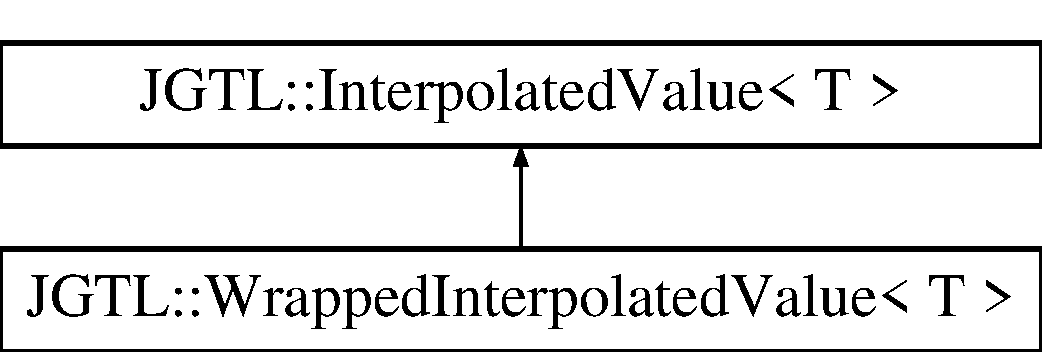
\includegraphics[height=2cm]{class_j_g_t_l_1_1_interpolated_value}
\end{center}
\end{figure}
\subsection*{Public Member Functions}
\begin{CompactItemize}
\item 
\hyperlink{class_j_g_t_l_1_1_interpolated_value_bccb0ff62b1196afd31d0fec4794f3e7}{Interpolated\-Value} ()
\item 
\hyperlink{class_j_g_t_l_1_1_interpolated_value_9664708ef92a7c352429c37d0f463f2f}{Interpolated\-Value} (float \_\-interpolation\-Coeff)
\item 
\hyperlink{class_j_g_t_l_1_1_interpolated_value_d8bccc51f6cb96e1bfe433d5b83a94ba}{Interpolated\-Value} (const T \&\_\-value, float \_\-interpolation\-Coeff)
\item 
const \hyperlink{class_j_g_t_l_1_1_interpolated_value}{Interpolated\-Value}$<$ T $>$ \& \hyperlink{class_j_g_t_l_1_1_interpolated_value_30b679bad94ef7adf003bf99e5756a53}{operator=} (T \_\-potential\-Value)
\item 
float \hyperlink{class_j_g_t_l_1_1_interpolated_value_79acd7ca199cd56a2930dd362f0e78ef}{get\-Interpolation\-Coeff} ()
\item 
void \hyperlink{class_j_g_t_l_1_1_interpolated_value_fbd2118a23563bf541c1388131035ef5}{set\-Coeff} (float \_\-coeff)
\item 
virtual void \hyperlink{class_j_g_t_l_1_1_interpolated_value_eaeff236b97efbf0c616333e1b94b210}{set\-Value} (const T \&\_\-value)
\item 
void \hyperlink{class_j_g_t_l_1_1_interpolated_value_58856554c17b6b4b815e2e74e0dc5b5b}{operator+=} (const T \&\_\-value)
\item 
void \hyperlink{class_j_g_t_l_1_1_interpolated_value_d8cd429d3c46e1a49c5791a60deb7570}{operator-=} (const T \&\_\-value)
\item 
const T \& \hyperlink{class_j_g_t_l_1_1_interpolated_value_a3f9c94d927a923eaab2d6cec96d4dd7}{get\-Potential\-Value} () const
\item 
const T \& \hyperlink{class_j_g_t_l_1_1_interpolated_value_7197bfe20e331bfa6be2cbe122b2ffba}{get\-Actual\-Value} () const
\item 
void \hyperlink{class_j_g_t_l_1_1_interpolated_value_3098413c5cb85973a20b7066a5ed3171}{force\-Value} ()
\item 
virtual void \hyperlink{class_j_g_t_l_1_1_interpolated_value_bc1a6a8d484921bc309289c400bf0fbe}{update} (int times=1)
\end{CompactItemize}
\subsection*{Protected Attributes}
\begin{CompactItemize}
\item 
T \hyperlink{class_j_g_t_l_1_1_interpolated_value_38e69e9add9640f5678a877ffd99ac4e}{potential\-Value}
\item 
T \hyperlink{class_j_g_t_l_1_1_interpolated_value_db402fa9ddb87fc80411e1bbbd88241f}{actual\-Value}
\item 
float \hyperlink{class_j_g_t_l_1_1_interpolated_value_5f7a5762a8a5cb68597b8fc1a406d9d0}{interpolation\-Coeff}
\end{CompactItemize}


\subsection{Detailed Description}
\subsubsection*{template$<$class T$>$ class JGTL::Interpolated\-Value$<$ T $>$}

The \hyperlink{class_j_g_t_l_1_1_interpolated_value}{Interpolated\-Value} Class handles values which approach a limit using the formula New\-Value = actual\-Value + (potential\-Value-actual\-Value)$\ast$interpolation\-Coeff;. 

\begin{Desc}
\item[Author:]Jason Gauci \end{Desc}
\begin{Desc}
\item[Date:]2008 \end{Desc}




\subsection{Constructor \& Destructor Documentation}
\hypertarget{class_j_g_t_l_1_1_interpolated_value_bccb0ff62b1196afd31d0fec4794f3e7}{
\index{JGTL::InterpolatedValue@{JGTL::Interpolated\-Value}!InterpolatedValue@{InterpolatedValue}}
\index{InterpolatedValue@{InterpolatedValue}!JGTL::InterpolatedValue@{JGTL::Interpolated\-Value}}
\subsubsection[InterpolatedValue]{\setlength{\rightskip}{0pt plus 5cm}template$<$class T$>$ \hyperlink{class_j_g_t_l_1_1_interpolated_value}{JGTL::Interpolated\-Value}$<$ T $>$::\hyperlink{class_j_g_t_l_1_1_interpolated_value}{Interpolated\-Value} ()\hspace{0.3cm}{\tt  \mbox{[}inline\mbox{]}}}}
\label{class_j_g_t_l_1_1_interpolated_value_bccb0ff62b1196afd31d0fec4794f3e7}


\hypertarget{class_j_g_t_l_1_1_interpolated_value_9664708ef92a7c352429c37d0f463f2f}{
\index{JGTL::InterpolatedValue@{JGTL::Interpolated\-Value}!InterpolatedValue@{InterpolatedValue}}
\index{InterpolatedValue@{InterpolatedValue}!JGTL::InterpolatedValue@{JGTL::Interpolated\-Value}}
\subsubsection[InterpolatedValue]{\setlength{\rightskip}{0pt plus 5cm}template$<$class T$>$ \hyperlink{class_j_g_t_l_1_1_interpolated_value}{JGTL::Interpolated\-Value}$<$ T $>$::\hyperlink{class_j_g_t_l_1_1_interpolated_value}{Interpolated\-Value} (float {\em \_\-interpolation\-Coeff})\hspace{0.3cm}{\tt  \mbox{[}inline\mbox{]}}}}
\label{class_j_g_t_l_1_1_interpolated_value_9664708ef92a7c352429c37d0f463f2f}


\hypertarget{class_j_g_t_l_1_1_interpolated_value_d8bccc51f6cb96e1bfe433d5b83a94ba}{
\index{JGTL::InterpolatedValue@{JGTL::Interpolated\-Value}!InterpolatedValue@{InterpolatedValue}}
\index{InterpolatedValue@{InterpolatedValue}!JGTL::InterpolatedValue@{JGTL::Interpolated\-Value}}
\subsubsection[InterpolatedValue]{\setlength{\rightskip}{0pt plus 5cm}template$<$class T$>$ \hyperlink{class_j_g_t_l_1_1_interpolated_value}{JGTL::Interpolated\-Value}$<$ T $>$::\hyperlink{class_j_g_t_l_1_1_interpolated_value}{Interpolated\-Value} (const T \& {\em \_\-value}, float {\em \_\-interpolation\-Coeff})\hspace{0.3cm}{\tt  \mbox{[}inline\mbox{]}}}}
\label{class_j_g_t_l_1_1_interpolated_value_d8bccc51f6cb96e1bfe433d5b83a94ba}




\subsection{Member Function Documentation}
\hypertarget{class_j_g_t_l_1_1_interpolated_value_30b679bad94ef7adf003bf99e5756a53}{
\index{JGTL::InterpolatedValue@{JGTL::Interpolated\-Value}!operator=@{operator=}}
\index{operator=@{operator=}!JGTL::InterpolatedValue@{JGTL::Interpolated\-Value}}
\subsubsection[operator=]{\setlength{\rightskip}{0pt plus 5cm}template$<$class T$>$ const \hyperlink{class_j_g_t_l_1_1_interpolated_value}{Interpolated\-Value}$<$T$>$\& \hyperlink{class_j_g_t_l_1_1_interpolated_value}{JGTL::Interpolated\-Value}$<$ T $>$::operator= (T {\em \_\-potential\-Value})\hspace{0.3cm}{\tt  \mbox{[}inline\mbox{]}}}}
\label{class_j_g_t_l_1_1_interpolated_value_30b679bad94ef7adf003bf99e5756a53}




Reimplemented in \hyperlink{class_j_g_t_l_1_1_wrapped_interpolated_value_0608de450007ab26e20cd9a680da7e84}{JGTL::Wrapped\-Interpolated\-Value$<$ T $>$}.\hypertarget{class_j_g_t_l_1_1_interpolated_value_79acd7ca199cd56a2930dd362f0e78ef}{
\index{JGTL::InterpolatedValue@{JGTL::Interpolated\-Value}!getInterpolationCoeff@{getInterpolationCoeff}}
\index{getInterpolationCoeff@{getInterpolationCoeff}!JGTL::InterpolatedValue@{JGTL::Interpolated\-Value}}
\subsubsection[getInterpolationCoeff]{\setlength{\rightskip}{0pt plus 5cm}template$<$class T$>$ float \hyperlink{class_j_g_t_l_1_1_interpolated_value}{JGTL::Interpolated\-Value}$<$ T $>$::get\-Interpolation\-Coeff ()\hspace{0.3cm}{\tt  \mbox{[}inline\mbox{]}}}}
\label{class_j_g_t_l_1_1_interpolated_value_79acd7ca199cd56a2930dd362f0e78ef}


\hypertarget{class_j_g_t_l_1_1_interpolated_value_fbd2118a23563bf541c1388131035ef5}{
\index{JGTL::InterpolatedValue@{JGTL::Interpolated\-Value}!setCoeff@{setCoeff}}
\index{setCoeff@{setCoeff}!JGTL::InterpolatedValue@{JGTL::Interpolated\-Value}}
\subsubsection[setCoeff]{\setlength{\rightskip}{0pt plus 5cm}template$<$class T$>$ void \hyperlink{class_j_g_t_l_1_1_interpolated_value}{JGTL::Interpolated\-Value}$<$ T $>$::set\-Coeff (float {\em \_\-coeff})\hspace{0.3cm}{\tt  \mbox{[}inline\mbox{]}}}}
\label{class_j_g_t_l_1_1_interpolated_value_fbd2118a23563bf541c1388131035ef5}


\hypertarget{class_j_g_t_l_1_1_interpolated_value_eaeff236b97efbf0c616333e1b94b210}{
\index{JGTL::InterpolatedValue@{JGTL::Interpolated\-Value}!setValue@{setValue}}
\index{setValue@{setValue}!JGTL::InterpolatedValue@{JGTL::Interpolated\-Value}}
\subsubsection[setValue]{\setlength{\rightskip}{0pt plus 5cm}template$<$class T$>$ virtual void \hyperlink{class_j_g_t_l_1_1_interpolated_value}{JGTL::Interpolated\-Value}$<$ T $>$::set\-Value (const T \& {\em \_\-value})\hspace{0.3cm}{\tt  \mbox{[}inline, virtual\mbox{]}}}}
\label{class_j_g_t_l_1_1_interpolated_value_eaeff236b97efbf0c616333e1b94b210}




Reimplemented in \hyperlink{class_j_g_t_l_1_1_wrapped_interpolated_value_1cc76107e67afe602b384a1ecc9e2840}{JGTL::Wrapped\-Interpolated\-Value$<$ T $>$}.\hypertarget{class_j_g_t_l_1_1_interpolated_value_58856554c17b6b4b815e2e74e0dc5b5b}{
\index{JGTL::InterpolatedValue@{JGTL::Interpolated\-Value}!operator+=@{operator+=}}
\index{operator+=@{operator+=}!JGTL::InterpolatedValue@{JGTL::Interpolated\-Value}}
\subsubsection[operator+=]{\setlength{\rightskip}{0pt plus 5cm}template$<$class T$>$ void \hyperlink{class_j_g_t_l_1_1_interpolated_value}{JGTL::Interpolated\-Value}$<$ T $>$::operator+= (const T \& {\em \_\-value})\hspace{0.3cm}{\tt  \mbox{[}inline\mbox{]}}}}
\label{class_j_g_t_l_1_1_interpolated_value_58856554c17b6b4b815e2e74e0dc5b5b}


\hypertarget{class_j_g_t_l_1_1_interpolated_value_d8cd429d3c46e1a49c5791a60deb7570}{
\index{JGTL::InterpolatedValue@{JGTL::Interpolated\-Value}!operator-=@{operator-=}}
\index{operator-=@{operator-=}!JGTL::InterpolatedValue@{JGTL::Interpolated\-Value}}
\subsubsection[operator-=]{\setlength{\rightskip}{0pt plus 5cm}template$<$class T$>$ void \hyperlink{class_j_g_t_l_1_1_interpolated_value}{JGTL::Interpolated\-Value}$<$ T $>$::operator-= (const T \& {\em \_\-value})\hspace{0.3cm}{\tt  \mbox{[}inline\mbox{]}}}}
\label{class_j_g_t_l_1_1_interpolated_value_d8cd429d3c46e1a49c5791a60deb7570}


\hypertarget{class_j_g_t_l_1_1_interpolated_value_a3f9c94d927a923eaab2d6cec96d4dd7}{
\index{JGTL::InterpolatedValue@{JGTL::Interpolated\-Value}!getPotentialValue@{getPotentialValue}}
\index{getPotentialValue@{getPotentialValue}!JGTL::InterpolatedValue@{JGTL::Interpolated\-Value}}
\subsubsection[getPotentialValue]{\setlength{\rightskip}{0pt plus 5cm}template$<$class T$>$ const T\& \hyperlink{class_j_g_t_l_1_1_interpolated_value}{JGTL::Interpolated\-Value}$<$ T $>$::get\-Potential\-Value () const\hspace{0.3cm}{\tt  \mbox{[}inline\mbox{]}}}}
\label{class_j_g_t_l_1_1_interpolated_value_a3f9c94d927a923eaab2d6cec96d4dd7}


\hypertarget{class_j_g_t_l_1_1_interpolated_value_7197bfe20e331bfa6be2cbe122b2ffba}{
\index{JGTL::InterpolatedValue@{JGTL::Interpolated\-Value}!getActualValue@{getActualValue}}
\index{getActualValue@{getActualValue}!JGTL::InterpolatedValue@{JGTL::Interpolated\-Value}}
\subsubsection[getActualValue]{\setlength{\rightskip}{0pt plus 5cm}template$<$class T$>$ const T\& \hyperlink{class_j_g_t_l_1_1_interpolated_value}{JGTL::Interpolated\-Value}$<$ T $>$::get\-Actual\-Value () const\hspace{0.3cm}{\tt  \mbox{[}inline\mbox{]}}}}
\label{class_j_g_t_l_1_1_interpolated_value_7197bfe20e331bfa6be2cbe122b2ffba}


\hypertarget{class_j_g_t_l_1_1_interpolated_value_3098413c5cb85973a20b7066a5ed3171}{
\index{JGTL::InterpolatedValue@{JGTL::Interpolated\-Value}!forceValue@{forceValue}}
\index{forceValue@{forceValue}!JGTL::InterpolatedValue@{JGTL::Interpolated\-Value}}
\subsubsection[forceValue]{\setlength{\rightskip}{0pt plus 5cm}template$<$class T$>$ void \hyperlink{class_j_g_t_l_1_1_interpolated_value}{JGTL::Interpolated\-Value}$<$ T $>$::force\-Value ()\hspace{0.3cm}{\tt  \mbox{[}inline\mbox{]}}}}
\label{class_j_g_t_l_1_1_interpolated_value_3098413c5cb85973a20b7066a5ed3171}


\hypertarget{class_j_g_t_l_1_1_interpolated_value_bc1a6a8d484921bc309289c400bf0fbe}{
\index{JGTL::InterpolatedValue@{JGTL::Interpolated\-Value}!update@{update}}
\index{update@{update}!JGTL::InterpolatedValue@{JGTL::Interpolated\-Value}}
\subsubsection[update]{\setlength{\rightskip}{0pt plus 5cm}template$<$class T$>$ virtual void \hyperlink{class_j_g_t_l_1_1_interpolated_value}{JGTL::Interpolated\-Value}$<$ T $>$::update (int {\em times} = {\tt 1})\hspace{0.3cm}{\tt  \mbox{[}inline, virtual\mbox{]}}}}
\label{class_j_g_t_l_1_1_interpolated_value_bc1a6a8d484921bc309289c400bf0fbe}




Reimplemented in \hyperlink{class_j_g_t_l_1_1_wrapped_interpolated_value_2bdc736eda165b27af022bae1f352aae}{JGTL::Wrapped\-Interpolated\-Value$<$ T $>$}.

\subsection{Member Data Documentation}
\hypertarget{class_j_g_t_l_1_1_interpolated_value_38e69e9add9640f5678a877ffd99ac4e}{
\index{JGTL::InterpolatedValue@{JGTL::Interpolated\-Value}!potentialValue@{potentialValue}}
\index{potentialValue@{potentialValue}!JGTL::InterpolatedValue@{JGTL::Interpolated\-Value}}
\subsubsection[potentialValue]{\setlength{\rightskip}{0pt plus 5cm}template$<$class T$>$ T \hyperlink{class_j_g_t_l_1_1_interpolated_value}{JGTL::Interpolated\-Value}$<$ T $>$::\hyperlink{class_j_g_t_l_1_1_interpolated_value_38e69e9add9640f5678a877ffd99ac4e}{potential\-Value}\hspace{0.3cm}{\tt  \mbox{[}protected\mbox{]}}}}
\label{class_j_g_t_l_1_1_interpolated_value_38e69e9add9640f5678a877ffd99ac4e}


\hypertarget{class_j_g_t_l_1_1_interpolated_value_db402fa9ddb87fc80411e1bbbd88241f}{
\index{JGTL::InterpolatedValue@{JGTL::Interpolated\-Value}!actualValue@{actualValue}}
\index{actualValue@{actualValue}!JGTL::InterpolatedValue@{JGTL::Interpolated\-Value}}
\subsubsection[actualValue]{\setlength{\rightskip}{0pt plus 5cm}template$<$class T$>$ T \hyperlink{class_j_g_t_l_1_1_interpolated_value}{JGTL::Interpolated\-Value}$<$ T $>$::\hyperlink{class_j_g_t_l_1_1_interpolated_value_db402fa9ddb87fc80411e1bbbd88241f}{actual\-Value}\hspace{0.3cm}{\tt  \mbox{[}protected\mbox{]}}}}
\label{class_j_g_t_l_1_1_interpolated_value_db402fa9ddb87fc80411e1bbbd88241f}


This is the current value. This value is approaching the potential value \hypertarget{class_j_g_t_l_1_1_interpolated_value_5f7a5762a8a5cb68597b8fc1a406d9d0}{
\index{JGTL::InterpolatedValue@{JGTL::Interpolated\-Value}!interpolationCoeff@{interpolationCoeff}}
\index{interpolationCoeff@{interpolationCoeff}!JGTL::InterpolatedValue@{JGTL::Interpolated\-Value}}
\subsubsection[interpolationCoeff]{\setlength{\rightskip}{0pt plus 5cm}template$<$class T$>$ float \hyperlink{class_j_g_t_l_1_1_interpolated_value}{JGTL::Interpolated\-Value}$<$ T $>$::\hyperlink{class_j_g_t_l_1_1_interpolated_value_5f7a5762a8a5cb68597b8fc1a406d9d0}{interpolation\-Coeff}\hspace{0.3cm}{\tt  \mbox{[}protected\mbox{]}}}}
\label{class_j_g_t_l_1_1_interpolated_value_5f7a5762a8a5cb68597b8fc1a406d9d0}


This handles the rate at which the actual value approaches the potential value 

The documentation for this class was generated from the following file:\begin{CompactItemize}
\item 
\hyperlink{_j_g_t_l___interpolated_value_8h}{JGTL\_\-Interpolated\-Value.h}\end{CompactItemize}

\hypertarget{class_j_g_t_l_1_1_located_exception}{
\section{JGTL::Located\-Exception Class Reference}
\label{class_j_g_t_l_1_1_located_exception}\index{JGTL::LocatedException@{JGTL::LocatedException}}
}
This class handles throwing exceptions which include the file and line number.  


{\tt \#include $<$JGTL\_\-Located\-Exception.h$>$}

\subsection*{Public Member Functions}
\begin{CompactItemize}
\item 
\hyperlink{class_j_g_t_l_1_1_located_exception_6dc12a4d8a6e75095fd87a45c2cfc54e}{Located\-Exception} (const char $\ast$\_\-reason, const char $\ast$\_\-file\-Name, const int \_\-line\-Number)
\item 
\hyperlink{class_j_g_t_l_1_1_located_exception_3204e4c6770b4f61dc063aa0e440dd9a}{Located\-Exception} (const std::string \&\_\-reason, const char $\ast$\_\-file\-Name, const int \_\-line\-Number)
\item 
virtual const char $\ast$ \hyperlink{class_j_g_t_l_1_1_located_exception_563583a831452b2e4a522ba943f8b6ed}{what} () const  throw ()
\end{CompactItemize}
\subsection*{Private Attributes}
\begin{CompactItemize}
\item 
char \hyperlink{class_j_g_t_l_1_1_located_exception_db8c3af227f50afffa775e69fe82b096}{text} \mbox{[}4096\mbox{]}
\end{CompactItemize}


\subsection{Detailed Description}
This class handles throwing exceptions which include the file and line number. 

Example:

throw CREATE\_\-LOCATEDEXCEPTION\_\-INFO(\char`\"{}ERROR!\char`\"{});

\begin{Desc}
\item[Author:]Jason Gauci \end{Desc}
\begin{Desc}
\item[Date:]2008 \end{Desc}




\subsection{Constructor \& Destructor Documentation}
\hypertarget{class_j_g_t_l_1_1_located_exception_6dc12a4d8a6e75095fd87a45c2cfc54e}{
\index{JGTL::LocatedException@{JGTL::Located\-Exception}!LocatedException@{LocatedException}}
\index{LocatedException@{LocatedException}!JGTL::LocatedException@{JGTL::Located\-Exception}}
\subsubsection[LocatedException]{\setlength{\rightskip}{0pt plus 5cm}JGTL::Located\-Exception::Located\-Exception (const char $\ast$ {\em \_\-reason}, const char $\ast$ {\em \_\-file\-Name}, const int {\em \_\-line\-Number})\hspace{0.3cm}{\tt  \mbox{[}inline\mbox{]}}}}
\label{class_j_g_t_l_1_1_located_exception_6dc12a4d8a6e75095fd87a45c2cfc54e}


\hypertarget{class_j_g_t_l_1_1_located_exception_3204e4c6770b4f61dc063aa0e440dd9a}{
\index{JGTL::LocatedException@{JGTL::Located\-Exception}!LocatedException@{LocatedException}}
\index{LocatedException@{LocatedException}!JGTL::LocatedException@{JGTL::Located\-Exception}}
\subsubsection[LocatedException]{\setlength{\rightskip}{0pt plus 5cm}JGTL::Located\-Exception::Located\-Exception (const std::string \& {\em \_\-reason}, const char $\ast$ {\em \_\-file\-Name}, const int {\em \_\-line\-Number})\hspace{0.3cm}{\tt  \mbox{[}inline\mbox{]}}}}
\label{class_j_g_t_l_1_1_located_exception_3204e4c6770b4f61dc063aa0e440dd9a}




\subsection{Member Function Documentation}
\hypertarget{class_j_g_t_l_1_1_located_exception_563583a831452b2e4a522ba943f8b6ed}{
\index{JGTL::LocatedException@{JGTL::Located\-Exception}!what@{what}}
\index{what@{what}!JGTL::LocatedException@{JGTL::Located\-Exception}}
\subsubsection[what]{\setlength{\rightskip}{0pt plus 5cm}virtual const char$\ast$ JGTL::Located\-Exception::what () const  throw ()\hspace{0.3cm}{\tt  \mbox{[}inline, virtual\mbox{]}}}}
\label{class_j_g_t_l_1_1_located_exception_563583a831452b2e4a522ba943f8b6ed}




\subsection{Member Data Documentation}
\hypertarget{class_j_g_t_l_1_1_located_exception_db8c3af227f50afffa775e69fe82b096}{
\index{JGTL::LocatedException@{JGTL::Located\-Exception}!text@{text}}
\index{text@{text}!JGTL::LocatedException@{JGTL::Located\-Exception}}
\subsubsection[text]{\setlength{\rightskip}{0pt plus 5cm}char \hyperlink{class_j_g_t_l_1_1_located_exception_db8c3af227f50afffa775e69fe82b096}{JGTL::Located\-Exception::text}\mbox{[}4096\mbox{]}\hspace{0.3cm}{\tt  \mbox{[}private\mbox{]}}}}
\label{class_j_g_t_l_1_1_located_exception_db8c3af227f50afffa775e69fe82b096}




The documentation for this class was generated from the following file:\begin{CompactItemize}
\item 
\hyperlink{_j_g_t_l___located_exception_8h}{JGTL\_\-Located\-Exception.h}\end{CompactItemize}

\hypertarget{class_j_g_t_l_1_1_map_interface}{
\section{JGTL::Map\-Interface$<$ Key, Data $>$ Class Template Reference}
\label{class_j_g_t_l_1_1_map_interface}\index{JGTL::MapInterface@{JGTL::MapInterface}}
}
This class acts as a base class for the Map construct.  


{\tt \#include $<$JGTL\_\-Map\-Interface.h$>$}

Inheritance diagram for JGTL::Map\-Interface$<$ Key, Data $>$::\begin{figure}[H]
\begin{center}
\leavevmode
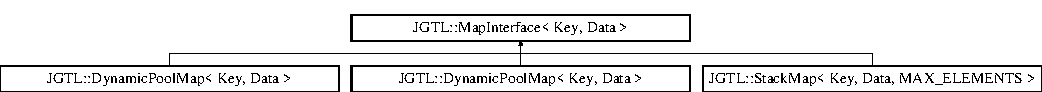
\includegraphics[height=1.22807cm]{class_j_g_t_l_1_1_map_interface}
\end{center}
\end{figure}
\subsection*{Public Types}
\begin{CompactItemize}
\item 
typedef std::pair$<$ Key, Data $>$ $\ast$ \hyperlink{class_j_g_t_l_1_1_map_interface_a8fcdbd899d0df84ce1aaa67d8dc000e}{iterator}
\item 
typedef const std::pair$<$ Key, Data $>$ $\ast$ \hyperlink{class_j_g_t_l_1_1_map_interface_bbce6cc516069a5a504e0ae5b9aecd88}{const\_\-iterator}
\item 
typedef std::pair$<$ Key, Data $>$ \hyperlink{class_j_g_t_l_1_1_map_interface_b7e9654bf9b2a906465e362475466ca5}{Tree\-Item}
\item 
typedef \hyperlink{class_j_g_t_l_1_1_binary_tree_node}{Binary\-Tree\-Node} \hyperlink{class_j_g_t_l_1_1_map_interface_0e980afab09f7663362337e025f73540}{Tree\-Node}
\end{CompactItemize}
\subsection*{Public Member Functions}
\begin{CompactItemize}
\item 
\hyperlink{class_j_g_t_l_1_1_map_interface_6d49e996123c82dbc4ac2b526de5225d}{Map\-Interface} ()
\item 
virtual \hyperlink{class_j_g_t_l_1_1_map_interface_f6fd6f5a7643f34cae4b7b67ba98a832}{$\sim$Map\-Interface} ()
\item 
bool \hyperlink{class_j_g_t_l_1_1_map_interface_2f61fdf95543ba566256642eeed659f4}{operator==} (const \hyperlink{class_j_g_t_l_1_1_map_interface}{Map\-Interface} \&other) const 
\item 
virtual bool \hyperlink{class_j_g_t_l_1_1_map_interface_177b75de36104c54e53080db65b777a2}{resize} (int new\-Size)=0
\item 
virtual void \hyperlink{class_j_g_t_l_1_1_map_interface_e416f8f15a065ea183c289932ef794c6}{insert} (const Key \&key, const Data \&data)
\item 
int \hyperlink{class_j_g_t_l_1_1_map_interface_416044d92d5c6d09ed79d13a775ba222}{size} () const
\item 
bool \hyperlink{class_j_g_t_l_1_1_map_interface_66e2355bebebd18fca84dee62e0fffa5}{empty} () const
\item 
void \hyperlink{class_j_g_t_l_1_1_map_interface_af2d3667a3a9cf577177720e2b757d03}{clear} ()
\item 
\hyperlink{class_j_g_t_l_1_1_map_interface_a8fcdbd899d0df84ce1aaa67d8dc000e}{iterator} \hyperlink{class_j_g_t_l_1_1_map_interface_b75e298063852903c54de5c9d17a2302}{begin} ()
\item 
\hyperlink{class_j_g_t_l_1_1_map_interface_bbce6cc516069a5a504e0ae5b9aecd88}{const\_\-iterator} \hyperlink{class_j_g_t_l_1_1_map_interface_38bbeb2dba7c6b3d8a8a2e6f441b1757}{begin} () const
\item 
\hyperlink{class_j_g_t_l_1_1_map_interface_a8fcdbd899d0df84ce1aaa67d8dc000e}{iterator} \hyperlink{class_j_g_t_l_1_1_map_interface_b942b543e93621e8e6a84c8fcadb29fc}{end} ()
\item 
\hyperlink{class_j_g_t_l_1_1_map_interface_bbce6cc516069a5a504e0ae5b9aecd88}{const\_\-iterator} \hyperlink{class_j_g_t_l_1_1_map_interface_8ce89dcb9cfb3d23d7123a8e7ad98633}{end} () const
\item 
const bool \hyperlink{class_j_g_t_l_1_1_map_interface_6a4c3571cb30d168d4a67dd2655a6b77}{has\-Key} (const Key \&key) const 
\item 
\hyperlink{class_j_g_t_l_1_1_map_interface_a8fcdbd899d0df84ce1aaa67d8dc000e}{iterator} \hyperlink{class_j_g_t_l_1_1_map_interface_7e97b54c29a253bd99caf2b0decb95a8}{find} (const Key \&key)
\item 
\hyperlink{class_j_g_t_l_1_1_map_interface_bbce6cc516069a5a504e0ae5b9aecd88}{const\_\-iterator} \hyperlink{class_j_g_t_l_1_1_map_interface_4ec2d9323c3d2e65179c38ea7558a222}{find} (const Key \&key) const 
\item 
Data $\ast$ \hyperlink{class_j_g_t_l_1_1_map_interface_b18a78bcb6d8ebac123e934aaa3fad0b}{get\-Data} (const Key \&key)
\item 
const Data $\ast$ \hyperlink{class_j_g_t_l_1_1_map_interface_266cbd67bcff93d17649c35254d18190}{get\-Data} (const Key \&key) const 
\item 
const Data \& \hyperlink{class_j_g_t_l_1_1_map_interface_3613d63a8096f923e4e220e5aa002403}{get\-Data\-Ref} (const Key \&key) const 
\item 
void \hyperlink{class_j_g_t_l_1_1_map_interface_7fe23525fa2fca5e47cb047332fb49d3}{erase} (\hyperlink{class_j_g_t_l_1_1_map_interface_bbce6cc516069a5a504e0ae5b9aecd88}{const\_\-iterator} iter)
\item 
void \hyperlink{class_j_g_t_l_1_1_map_interface_8b9cf8f1daa77edaf645c22f81812fcf}{erase\-Index} (int index)
\item 
const Data \& \hyperlink{class_j_g_t_l_1_1_map_interface_3bd1eca8bba2b057e09eb6579e26ad8f}{get\-Index\-Data} (int index) const
\item 
Data $\ast$ \hyperlink{class_j_g_t_l_1_1_map_interface_e2b0ad1f3959cf7f8d1c6ef07c5a8c2c}{get\-Index\-Data\-Ptr} (int index)
\item 
const Data $\ast$ \hyperlink{class_j_g_t_l_1_1_map_interface_cbbfe062862b57f4e0027026f81562a9}{get\-Index\-Data\-Ptr} (int index) const
\item 
const std::pair$<$ Key, Data $>$ \& \hyperlink{class_j_g_t_l_1_1_map_interface_2fad30d3c69882b66d210539775db665}{get\-Index} (int index) const
\item 
\hyperlink{class_j_g_t_l_1_1_map_interface_a8fcdbd899d0df84ce1aaa67d8dc000e}{iterator} \hyperlink{class_j_g_t_l_1_1_map_interface_1d28999130a2279ae668715e90ae5529}{get\-Index\-Ptr} (int index)
\item 
\hyperlink{class_j_g_t_l_1_1_map_interface_bbce6cc516069a5a504e0ae5b9aecd88}{const\_\-iterator} \hyperlink{class_j_g_t_l_1_1_map_interface_f5cfdb7ca92b031a3ec4835c02a64d97}{get\-Index\-Ptr} (int index) const
\item 
\hyperlink{class_j_g_t_l_1_1_map_interface_6d49e996123c82dbc4ac2b526de5225d}{Map\-Interface} ()
\item 
virtual \hyperlink{class_j_g_t_l_1_1_map_interface_f6fd6f5a7643f34cae4b7b67ba98a832}{$\sim$Map\-Interface} ()
\item 
bool \hyperlink{class_j_g_t_l_1_1_map_interface_2f61fdf95543ba566256642eeed659f4}{operator==} (const \hyperlink{class_j_g_t_l_1_1_map_interface}{Map\-Interface} \&other) const 
\item 
virtual bool \hyperlink{class_j_g_t_l_1_1_map_interface_d5d7c32e4e413ef6fcd93ca53951ecf8}{reserve} (int new\-Size)
\item 
virtual void \hyperlink{class_j_g_t_l_1_1_map_interface_e416f8f15a065ea183c289932ef794c6}{insert} (const Key \&key, const Data \&data)
\item 
int \hyperlink{class_j_g_t_l_1_1_map_interface_416044d92d5c6d09ed79d13a775ba222}{size} () const
\item 
void \hyperlink{class_j_g_t_l_1_1_map_interface_af2d3667a3a9cf577177720e2b757d03}{clear} ()
\item 
const bool \hyperlink{class_j_g_t_l_1_1_map_interface_6a4c3571cb30d168d4a67dd2655a6b77}{has\-Key} (const Key \&key) const 
\item 
\hyperlink{class_j_g_t_l_1_1_map_interface_a8fcdbd899d0df84ce1aaa67d8dc000e}{iterator} \hyperlink{class_j_g_t_l_1_1_map_interface_7e97b54c29a253bd99caf2b0decb95a8}{find} (const Key \&key)
\item 
\hyperlink{class_j_g_t_l_1_1_map_interface_bbce6cc516069a5a504e0ae5b9aecd88}{const\_\-iterator} \hyperlink{class_j_g_t_l_1_1_map_interface_4ec2d9323c3d2e65179c38ea7558a222}{find} (const Key \&key) const 
\item 
Data $\ast$ \hyperlink{class_j_g_t_l_1_1_map_interface_b18a78bcb6d8ebac123e934aaa3fad0b}{get\-Data} (const Key \&key)
\item 
const Data $\ast$ \hyperlink{class_j_g_t_l_1_1_map_interface_266cbd67bcff93d17649c35254d18190}{get\-Data} (const Key \&key) const 
\item 
const Data \& \hyperlink{class_j_g_t_l_1_1_map_interface_3613d63a8096f923e4e220e5aa002403}{get\-Data\-Ref} (const Key \&key) const 
\item 
void \hyperlink{class_j_g_t_l_1_1_map_interface_7fe23525fa2fca5e47cb047332fb49d3}{erase} (\hyperlink{class_j_g_t_l_1_1_map_interface_bbce6cc516069a5a504e0ae5b9aecd88}{const\_\-iterator} iter)
\item 
const Data \& \hyperlink{class_j_g_t_l_1_1_map_interface_3bd1eca8bba2b057e09eb6579e26ad8f}{get\-Index\-Data} (int index) const
\item 
Data $\ast$ \hyperlink{class_j_g_t_l_1_1_map_interface_e2b0ad1f3959cf7f8d1c6ef07c5a8c2c}{get\-Index\-Data\-Ptr} (int index)
\item 
const Data $\ast$ \hyperlink{class_j_g_t_l_1_1_map_interface_cbbfe062862b57f4e0027026f81562a9}{get\-Index\-Data\-Ptr} (int index) const
\end{CompactItemize}
\subsection*{Protected Attributes}
\begin{CompactItemize}
\item 
int \hyperlink{class_j_g_t_l_1_1_map_interface_02b41b644ec9f7fc80888f2a621262e3}{num\-Elements}
\item 
int \hyperlink{class_j_g_t_l_1_1_map_interface_fd420367e3791206e3f22e9610e21afc}{max\-Elements}
\item 
std::pair$<$ Key, Data $>$ $\ast$ \hyperlink{class_j_g_t_l_1_1_map_interface_b2f183b5fa7244a2b85571c2a62235c1}{data\-List}
\item 
\hyperlink{class_j_g_t_l_1_1_map_interface_b7e9654bf9b2a906465e362475466ca5}{Tree\-Item} $\ast$ \hyperlink{class_j_g_t_l_1_1_map_interface_86fa704452e650dac12e3d01804739c2}{data\-List}
\item 
\hyperlink{class_j_g_t_l_1_1_binary_tree_node}{Tree\-Node} $\ast$ \hyperlink{class_j_g_t_l_1_1_map_interface_7b271ddce20b3fc8386360ca277da4fa}{node\-List}
\item 
int \hyperlink{class_j_g_t_l_1_1_map_interface_9407ca6114c7972d533f22ad1061e23b}{root\-Index}
\end{CompactItemize}


\subsection{Detailed Description}
\subsubsection*{template$<$class Key, class Data$>$ class JGTL::Map\-Interface$<$ Key, Data $>$}

This class acts as a base class for the Map construct. 

\begin{Desc}
\item[Author:]Jason Gauci \end{Desc}
\begin{Desc}
\item[Date:]2008 \end{Desc}




\subsection{Member Typedef Documentation}
\hypertarget{class_j_g_t_l_1_1_map_interface_a8fcdbd899d0df84ce1aaa67d8dc000e}{
\index{JGTL::MapInterface@{JGTL::Map\-Interface}!iterator@{iterator}}
\index{iterator@{iterator}!JGTL::MapInterface@{JGTL::Map\-Interface}}
\subsubsection[iterator]{\setlength{\rightskip}{0pt plus 5cm}template$<$class Key, class Data$>$ typedef std::pair$<$Key,Data$>$$\ast$ \hyperlink{class_j_g_t_l_1_1_map_interface}{JGTL::Map\-Interface}$<$ Key, Data $>$::\hyperlink{class_j_g_t_l_1_1_map_interface_a8fcdbd899d0df84ce1aaa67d8dc000e}{iterator}}}
\label{class_j_g_t_l_1_1_map_interface_a8fcdbd899d0df84ce1aaa67d8dc000e}


\hypertarget{class_j_g_t_l_1_1_map_interface_bbce6cc516069a5a504e0ae5b9aecd88}{
\index{JGTL::MapInterface@{JGTL::Map\-Interface}!const_iterator@{const\_\-iterator}}
\index{const_iterator@{const\_\-iterator}!JGTL::MapInterface@{JGTL::Map\-Interface}}
\subsubsection[const\_\-iterator]{\setlength{\rightskip}{0pt plus 5cm}template$<$class Key, class Data$>$ typedef const std::pair$<$Key,Data$>$$\ast$ \hyperlink{class_j_g_t_l_1_1_map_interface}{JGTL::Map\-Interface}$<$ Key, Data $>$::\hyperlink{class_j_g_t_l_1_1_map_interface_bbce6cc516069a5a504e0ae5b9aecd88}{const\_\-iterator}}}
\label{class_j_g_t_l_1_1_map_interface_bbce6cc516069a5a504e0ae5b9aecd88}


\hypertarget{class_j_g_t_l_1_1_map_interface_b7e9654bf9b2a906465e362475466ca5}{
\index{JGTL::MapInterface@{JGTL::Map\-Interface}!TreeItem@{TreeItem}}
\index{TreeItem@{TreeItem}!JGTL::MapInterface@{JGTL::Map\-Interface}}
\subsubsection[TreeItem]{\setlength{\rightskip}{0pt plus 5cm}template$<$class Key, class Data$>$ typedef std::pair$<$Key,Data$>$ \hyperlink{class_j_g_t_l_1_1_map_interface}{JGTL::Map\-Interface}$<$ Key, Data $>$::\hyperlink{class_j_g_t_l_1_1_map_interface_b7e9654bf9b2a906465e362475466ca5}{Tree\-Item}}}
\label{class_j_g_t_l_1_1_map_interface_b7e9654bf9b2a906465e362475466ca5}


\hypertarget{class_j_g_t_l_1_1_map_interface_0e980afab09f7663362337e025f73540}{
\index{JGTL::MapInterface@{JGTL::Map\-Interface}!TreeNode@{TreeNode}}
\index{TreeNode@{TreeNode}!JGTL::MapInterface@{JGTL::Map\-Interface}}
\subsubsection[TreeNode]{\setlength{\rightskip}{0pt plus 5cm}template$<$class Key, class Data$>$ typedef \hyperlink{class_j_g_t_l_1_1_binary_tree_node}{Binary\-Tree\-Node} \hyperlink{class_j_g_t_l_1_1_map_interface}{JGTL::Map\-Interface}$<$ Key, Data $>$::\hyperlink{class_j_g_t_l_1_1_binary_tree_node}{Tree\-Node}}}
\label{class_j_g_t_l_1_1_map_interface_0e980afab09f7663362337e025f73540}




\subsection{Constructor \& Destructor Documentation}
\hypertarget{class_j_g_t_l_1_1_map_interface_6d49e996123c82dbc4ac2b526de5225d}{
\index{JGTL::MapInterface@{JGTL::Map\-Interface}!MapInterface@{MapInterface}}
\index{MapInterface@{MapInterface}!JGTL::MapInterface@{JGTL::Map\-Interface}}
\subsubsection[MapInterface]{\setlength{\rightskip}{0pt plus 5cm}template$<$class Key, class Data$>$ \hyperlink{class_j_g_t_l_1_1_map_interface}{JGTL::Map\-Interface}$<$ Key, Data $>$::\hyperlink{class_j_g_t_l_1_1_map_interface}{Map\-Interface} ()\hspace{0.3cm}{\tt  \mbox{[}inline\mbox{]}}}}
\label{class_j_g_t_l_1_1_map_interface_6d49e996123c82dbc4ac2b526de5225d}


\hypertarget{class_j_g_t_l_1_1_map_interface_f6fd6f5a7643f34cae4b7b67ba98a832}{
\index{JGTL::MapInterface@{JGTL::Map\-Interface}!~MapInterface@{$\sim$MapInterface}}
\index{~MapInterface@{$\sim$MapInterface}!JGTL::MapInterface@{JGTL::Map\-Interface}}
\subsubsection[$\sim$MapInterface]{\setlength{\rightskip}{0pt plus 5cm}template$<$class Key, class Data$>$ virtual \hyperlink{class_j_g_t_l_1_1_map_interface}{JGTL::Map\-Interface}$<$ Key, Data $>$::$\sim$\hyperlink{class_j_g_t_l_1_1_map_interface}{Map\-Interface} ()\hspace{0.3cm}{\tt  \mbox{[}inline, virtual\mbox{]}}}}
\label{class_j_g_t_l_1_1_map_interface_f6fd6f5a7643f34cae4b7b67ba98a832}


\hypertarget{class_j_g_t_l_1_1_map_interface_6d49e996123c82dbc4ac2b526de5225d}{
\index{JGTL::MapInterface@{JGTL::Map\-Interface}!MapInterface@{MapInterface}}
\index{MapInterface@{MapInterface}!JGTL::MapInterface@{JGTL::Map\-Interface}}
\subsubsection[MapInterface]{\setlength{\rightskip}{0pt plus 5cm}template$<$class Key, class Data$>$ \hyperlink{class_j_g_t_l_1_1_map_interface}{JGTL::Map\-Interface}$<$ Key, Data $>$::\hyperlink{class_j_g_t_l_1_1_map_interface}{Map\-Interface} ()\hspace{0.3cm}{\tt  \mbox{[}inline\mbox{]}}}}
\label{class_j_g_t_l_1_1_map_interface_6d49e996123c82dbc4ac2b526de5225d}


\hypertarget{class_j_g_t_l_1_1_map_interface_f6fd6f5a7643f34cae4b7b67ba98a832}{
\index{JGTL::MapInterface@{JGTL::Map\-Interface}!~MapInterface@{$\sim$MapInterface}}
\index{~MapInterface@{$\sim$MapInterface}!JGTL::MapInterface@{JGTL::Map\-Interface}}
\subsubsection[$\sim$MapInterface]{\setlength{\rightskip}{0pt plus 5cm}template$<$class Key, class Data$>$ virtual \hyperlink{class_j_g_t_l_1_1_map_interface}{JGTL::Map\-Interface}$<$ Key, Data $>$::$\sim$\hyperlink{class_j_g_t_l_1_1_map_interface}{Map\-Interface} ()\hspace{0.3cm}{\tt  \mbox{[}inline, virtual\mbox{]}}}}
\label{class_j_g_t_l_1_1_map_interface_f6fd6f5a7643f34cae4b7b67ba98a832}




\subsection{Member Function Documentation}
\hypertarget{class_j_g_t_l_1_1_map_interface_2f61fdf95543ba566256642eeed659f4}{
\index{JGTL::MapInterface@{JGTL::Map\-Interface}!operator==@{operator==}}
\index{operator==@{operator==}!JGTL::MapInterface@{JGTL::Map\-Interface}}
\subsubsection[operator==]{\setlength{\rightskip}{0pt plus 5cm}template$<$class Key, class Data$>$ bool \hyperlink{class_j_g_t_l_1_1_map_interface}{JGTL::Map\-Interface}$<$ Key, Data $>$::operator== (const \hyperlink{class_j_g_t_l_1_1_map_interface}{Map\-Interface}$<$ Key, Data $>$ \& {\em other}) const\hspace{0.3cm}{\tt  \mbox{[}inline\mbox{]}}}}
\label{class_j_g_t_l_1_1_map_interface_2f61fdf95543ba566256642eeed659f4}


\hypertarget{class_j_g_t_l_1_1_map_interface_177b75de36104c54e53080db65b777a2}{
\index{JGTL::MapInterface@{JGTL::Map\-Interface}!resize@{resize}}
\index{resize@{resize}!JGTL::MapInterface@{JGTL::Map\-Interface}}
\subsubsection[resize]{\setlength{\rightskip}{0pt plus 5cm}template$<$class Key, class Data$>$ virtual bool \hyperlink{class_j_g_t_l_1_1_map_interface}{JGTL::Map\-Interface}$<$ Key, Data $>$::resize (int {\em new\-Size})\hspace{0.3cm}{\tt  \mbox{[}pure virtual\mbox{]}}}}
\label{class_j_g_t_l_1_1_map_interface_177b75de36104c54e53080db65b777a2}




Implemented in \hyperlink{class_j_g_t_l_1_1_dynamic_pool_map_236509cad797d15cbed5e09adf356a04}{JGTL::Dynamic\-Pool\-Map$<$ Key, Data $>$}, \hyperlink{class_j_g_t_l_1_1_stack_map_cd9363efffeb00f6b48b21ed2685ac7c}{JGTL::Stack\-Map$<$ Key, Data, MAX\_\-ELEMENTS $>$}, and \hyperlink{class_j_g_t_l_1_1_dynamic_pool_map_236509cad797d15cbed5e09adf356a04}{JGTL::Dynamic\-Pool\-Map$<$ std::string, JGTL::Profile\-Block $\ast$ $>$}.\hypertarget{class_j_g_t_l_1_1_map_interface_e416f8f15a065ea183c289932ef794c6}{
\index{JGTL::MapInterface@{JGTL::Map\-Interface}!insert@{insert}}
\index{insert@{insert}!JGTL::MapInterface@{JGTL::Map\-Interface}}
\subsubsection[insert]{\setlength{\rightskip}{0pt plus 5cm}template$<$class Key, class Data$>$ virtual void \hyperlink{class_j_g_t_l_1_1_map_interface}{JGTL::Map\-Interface}$<$ Key, Data $>$::insert (const Key \& {\em key}, const Data \& {\em data})\hspace{0.3cm}{\tt  \mbox{[}inline, virtual\mbox{]}}}}
\label{class_j_g_t_l_1_1_map_interface_e416f8f15a065ea183c289932ef794c6}


\hypertarget{class_j_g_t_l_1_1_map_interface_416044d92d5c6d09ed79d13a775ba222}{
\index{JGTL::MapInterface@{JGTL::Map\-Interface}!size@{size}}
\index{size@{size}!JGTL::MapInterface@{JGTL::Map\-Interface}}
\subsubsection[size]{\setlength{\rightskip}{0pt plus 5cm}template$<$class Key, class Data$>$ int \hyperlink{class_j_g_t_l_1_1_map_interface}{JGTL::Map\-Interface}$<$ Key, Data $>$::size () const\hspace{0.3cm}{\tt  \mbox{[}inline\mbox{]}}}}
\label{class_j_g_t_l_1_1_map_interface_416044d92d5c6d09ed79d13a775ba222}


\hypertarget{class_j_g_t_l_1_1_map_interface_66e2355bebebd18fca84dee62e0fffa5}{
\index{JGTL::MapInterface@{JGTL::Map\-Interface}!empty@{empty}}
\index{empty@{empty}!JGTL::MapInterface@{JGTL::Map\-Interface}}
\subsubsection[empty]{\setlength{\rightskip}{0pt plus 5cm}template$<$class Key, class Data$>$ bool \hyperlink{class_j_g_t_l_1_1_map_interface}{JGTL::Map\-Interface}$<$ Key, Data $>$::empty () const\hspace{0.3cm}{\tt  \mbox{[}inline\mbox{]}}}}
\label{class_j_g_t_l_1_1_map_interface_66e2355bebebd18fca84dee62e0fffa5}


\hypertarget{class_j_g_t_l_1_1_map_interface_af2d3667a3a9cf577177720e2b757d03}{
\index{JGTL::MapInterface@{JGTL::Map\-Interface}!clear@{clear}}
\index{clear@{clear}!JGTL::MapInterface@{JGTL::Map\-Interface}}
\subsubsection[clear]{\setlength{\rightskip}{0pt plus 5cm}template$<$class Key, class Data$>$ void \hyperlink{class_j_g_t_l_1_1_map_interface}{JGTL::Map\-Interface}$<$ Key, Data $>$::clear ()\hspace{0.3cm}{\tt  \mbox{[}inline\mbox{]}}}}
\label{class_j_g_t_l_1_1_map_interface_af2d3667a3a9cf577177720e2b757d03}


\hypertarget{class_j_g_t_l_1_1_map_interface_b75e298063852903c54de5c9d17a2302}{
\index{JGTL::MapInterface@{JGTL::Map\-Interface}!begin@{begin}}
\index{begin@{begin}!JGTL::MapInterface@{JGTL::Map\-Interface}}
\subsubsection[begin]{\setlength{\rightskip}{0pt plus 5cm}template$<$class Key, class Data$>$ \hyperlink{class_j_g_t_l_1_1_map_interface_a8fcdbd899d0df84ce1aaa67d8dc000e}{iterator} \hyperlink{class_j_g_t_l_1_1_map_interface}{JGTL::Map\-Interface}$<$ Key, Data $>$::begin ()\hspace{0.3cm}{\tt  \mbox{[}inline\mbox{]}}}}
\label{class_j_g_t_l_1_1_map_interface_b75e298063852903c54de5c9d17a2302}


\hypertarget{class_j_g_t_l_1_1_map_interface_38bbeb2dba7c6b3d8a8a2e6f441b1757}{
\index{JGTL::MapInterface@{JGTL::Map\-Interface}!begin@{begin}}
\index{begin@{begin}!JGTL::MapInterface@{JGTL::Map\-Interface}}
\subsubsection[begin]{\setlength{\rightskip}{0pt plus 5cm}template$<$class Key, class Data$>$ \hyperlink{class_j_g_t_l_1_1_map_interface_bbce6cc516069a5a504e0ae5b9aecd88}{const\_\-iterator} \hyperlink{class_j_g_t_l_1_1_map_interface}{JGTL::Map\-Interface}$<$ Key, Data $>$::begin () const\hspace{0.3cm}{\tt  \mbox{[}inline\mbox{]}}}}
\label{class_j_g_t_l_1_1_map_interface_38bbeb2dba7c6b3d8a8a2e6f441b1757}


\hypertarget{class_j_g_t_l_1_1_map_interface_b942b543e93621e8e6a84c8fcadb29fc}{
\index{JGTL::MapInterface@{JGTL::Map\-Interface}!end@{end}}
\index{end@{end}!JGTL::MapInterface@{JGTL::Map\-Interface}}
\subsubsection[end]{\setlength{\rightskip}{0pt plus 5cm}template$<$class Key, class Data$>$ \hyperlink{class_j_g_t_l_1_1_map_interface_a8fcdbd899d0df84ce1aaa67d8dc000e}{iterator} \hyperlink{class_j_g_t_l_1_1_map_interface}{JGTL::Map\-Interface}$<$ Key, Data $>$::end ()\hspace{0.3cm}{\tt  \mbox{[}inline\mbox{]}}}}
\label{class_j_g_t_l_1_1_map_interface_b942b543e93621e8e6a84c8fcadb29fc}


\hypertarget{class_j_g_t_l_1_1_map_interface_8ce89dcb9cfb3d23d7123a8e7ad98633}{
\index{JGTL::MapInterface@{JGTL::Map\-Interface}!end@{end}}
\index{end@{end}!JGTL::MapInterface@{JGTL::Map\-Interface}}
\subsubsection[end]{\setlength{\rightskip}{0pt plus 5cm}template$<$class Key, class Data$>$ \hyperlink{class_j_g_t_l_1_1_map_interface_bbce6cc516069a5a504e0ae5b9aecd88}{const\_\-iterator} \hyperlink{class_j_g_t_l_1_1_map_interface}{JGTL::Map\-Interface}$<$ Key, Data $>$::end () const\hspace{0.3cm}{\tt  \mbox{[}inline\mbox{]}}}}
\label{class_j_g_t_l_1_1_map_interface_8ce89dcb9cfb3d23d7123a8e7ad98633}


\hypertarget{class_j_g_t_l_1_1_map_interface_6a4c3571cb30d168d4a67dd2655a6b77}{
\index{JGTL::MapInterface@{JGTL::Map\-Interface}!hasKey@{hasKey}}
\index{hasKey@{hasKey}!JGTL::MapInterface@{JGTL::Map\-Interface}}
\subsubsection[hasKey]{\setlength{\rightskip}{0pt plus 5cm}template$<$class Key, class Data$>$ const bool \hyperlink{class_j_g_t_l_1_1_map_interface}{JGTL::Map\-Interface}$<$ Key, Data $>$::has\-Key (const Key \& {\em key}) const\hspace{0.3cm}{\tt  \mbox{[}inline\mbox{]}}}}
\label{class_j_g_t_l_1_1_map_interface_6a4c3571cb30d168d4a67dd2655a6b77}


\hypertarget{class_j_g_t_l_1_1_map_interface_7e97b54c29a253bd99caf2b0decb95a8}{
\index{JGTL::MapInterface@{JGTL::Map\-Interface}!find@{find}}
\index{find@{find}!JGTL::MapInterface@{JGTL::Map\-Interface}}
\subsubsection[find]{\setlength{\rightskip}{0pt plus 5cm}template$<$class Key, class Data$>$ \hyperlink{class_j_g_t_l_1_1_map_interface_a8fcdbd899d0df84ce1aaa67d8dc000e}{iterator} \hyperlink{class_j_g_t_l_1_1_map_interface}{JGTL::Map\-Interface}$<$ Key, Data $>$::find (const Key \& {\em key})\hspace{0.3cm}{\tt  \mbox{[}inline\mbox{]}}}}
\label{class_j_g_t_l_1_1_map_interface_7e97b54c29a253bd99caf2b0decb95a8}


\hypertarget{class_j_g_t_l_1_1_map_interface_4ec2d9323c3d2e65179c38ea7558a222}{
\index{JGTL::MapInterface@{JGTL::Map\-Interface}!find@{find}}
\index{find@{find}!JGTL::MapInterface@{JGTL::Map\-Interface}}
\subsubsection[find]{\setlength{\rightskip}{0pt plus 5cm}template$<$class Key, class Data$>$ \hyperlink{class_j_g_t_l_1_1_map_interface_bbce6cc516069a5a504e0ae5b9aecd88}{const\_\-iterator} \hyperlink{class_j_g_t_l_1_1_map_interface}{JGTL::Map\-Interface}$<$ Key, Data $>$::find (const Key \& {\em key}) const\hspace{0.3cm}{\tt  \mbox{[}inline\mbox{]}}}}
\label{class_j_g_t_l_1_1_map_interface_4ec2d9323c3d2e65179c38ea7558a222}


\hypertarget{class_j_g_t_l_1_1_map_interface_b18a78bcb6d8ebac123e934aaa3fad0b}{
\index{JGTL::MapInterface@{JGTL::Map\-Interface}!getData@{getData}}
\index{getData@{getData}!JGTL::MapInterface@{JGTL::Map\-Interface}}
\subsubsection[getData]{\setlength{\rightskip}{0pt plus 5cm}template$<$class Key, class Data$>$ Data$\ast$ \hyperlink{class_j_g_t_l_1_1_map_interface}{JGTL::Map\-Interface}$<$ Key, Data $>$::get\-Data (const Key \& {\em key})\hspace{0.3cm}{\tt  \mbox{[}inline\mbox{]}}}}
\label{class_j_g_t_l_1_1_map_interface_b18a78bcb6d8ebac123e934aaa3fad0b}


\hypertarget{class_j_g_t_l_1_1_map_interface_266cbd67bcff93d17649c35254d18190}{
\index{JGTL::MapInterface@{JGTL::Map\-Interface}!getData@{getData}}
\index{getData@{getData}!JGTL::MapInterface@{JGTL::Map\-Interface}}
\subsubsection[getData]{\setlength{\rightskip}{0pt plus 5cm}template$<$class Key, class Data$>$ const Data$\ast$ \hyperlink{class_j_g_t_l_1_1_map_interface}{JGTL::Map\-Interface}$<$ Key, Data $>$::get\-Data (const Key \& {\em key}) const\hspace{0.3cm}{\tt  \mbox{[}inline\mbox{]}}}}
\label{class_j_g_t_l_1_1_map_interface_266cbd67bcff93d17649c35254d18190}


\hypertarget{class_j_g_t_l_1_1_map_interface_3613d63a8096f923e4e220e5aa002403}{
\index{JGTL::MapInterface@{JGTL::Map\-Interface}!getDataRef@{getDataRef}}
\index{getDataRef@{getDataRef}!JGTL::MapInterface@{JGTL::Map\-Interface}}
\subsubsection[getDataRef]{\setlength{\rightskip}{0pt plus 5cm}template$<$class Key, class Data$>$ const Data\& \hyperlink{class_j_g_t_l_1_1_map_interface}{JGTL::Map\-Interface}$<$ Key, Data $>$::get\-Data\-Ref (const Key \& {\em key}) const\hspace{0.3cm}{\tt  \mbox{[}inline\mbox{]}}}}
\label{class_j_g_t_l_1_1_map_interface_3613d63a8096f923e4e220e5aa002403}


\hypertarget{class_j_g_t_l_1_1_map_interface_7fe23525fa2fca5e47cb047332fb49d3}{
\index{JGTL::MapInterface@{JGTL::Map\-Interface}!erase@{erase}}
\index{erase@{erase}!JGTL::MapInterface@{JGTL::Map\-Interface}}
\subsubsection[erase]{\setlength{\rightskip}{0pt plus 5cm}template$<$class Key, class Data$>$ void \hyperlink{class_j_g_t_l_1_1_map_interface}{JGTL::Map\-Interface}$<$ Key, Data $>$::erase (\hyperlink{class_j_g_t_l_1_1_map_interface_bbce6cc516069a5a504e0ae5b9aecd88}{const\_\-iterator} {\em iter})\hspace{0.3cm}{\tt  \mbox{[}inline\mbox{]}}}}
\label{class_j_g_t_l_1_1_map_interface_7fe23525fa2fca5e47cb047332fb49d3}


\hypertarget{class_j_g_t_l_1_1_map_interface_8b9cf8f1daa77edaf645c22f81812fcf}{
\index{JGTL::MapInterface@{JGTL::Map\-Interface}!eraseIndex@{eraseIndex}}
\index{eraseIndex@{eraseIndex}!JGTL::MapInterface@{JGTL::Map\-Interface}}
\subsubsection[eraseIndex]{\setlength{\rightskip}{0pt plus 5cm}template$<$class Key, class Data$>$ void \hyperlink{class_j_g_t_l_1_1_map_interface}{JGTL::Map\-Interface}$<$ Key, Data $>$::erase\-Index (int {\em index})\hspace{0.3cm}{\tt  \mbox{[}inline\mbox{]}}}}
\label{class_j_g_t_l_1_1_map_interface_8b9cf8f1daa77edaf645c22f81812fcf}


\hypertarget{class_j_g_t_l_1_1_map_interface_3bd1eca8bba2b057e09eb6579e26ad8f}{
\index{JGTL::MapInterface@{JGTL::Map\-Interface}!getIndexData@{getIndexData}}
\index{getIndexData@{getIndexData}!JGTL::MapInterface@{JGTL::Map\-Interface}}
\subsubsection[getIndexData]{\setlength{\rightskip}{0pt plus 5cm}template$<$class Key, class Data$>$ const Data\& \hyperlink{class_j_g_t_l_1_1_map_interface}{JGTL::Map\-Interface}$<$ Key, Data $>$::get\-Index\-Data (int {\em index}) const\hspace{0.3cm}{\tt  \mbox{[}inline\mbox{]}}}}
\label{class_j_g_t_l_1_1_map_interface_3bd1eca8bba2b057e09eb6579e26ad8f}


\hypertarget{class_j_g_t_l_1_1_map_interface_e2b0ad1f3959cf7f8d1c6ef07c5a8c2c}{
\index{JGTL::MapInterface@{JGTL::Map\-Interface}!getIndexDataPtr@{getIndexDataPtr}}
\index{getIndexDataPtr@{getIndexDataPtr}!JGTL::MapInterface@{JGTL::Map\-Interface}}
\subsubsection[getIndexDataPtr]{\setlength{\rightskip}{0pt plus 5cm}template$<$class Key, class Data$>$ Data$\ast$ \hyperlink{class_j_g_t_l_1_1_map_interface}{JGTL::Map\-Interface}$<$ Key, Data $>$::get\-Index\-Data\-Ptr (int {\em index})\hspace{0.3cm}{\tt  \mbox{[}inline\mbox{]}}}}
\label{class_j_g_t_l_1_1_map_interface_e2b0ad1f3959cf7f8d1c6ef07c5a8c2c}


\hypertarget{class_j_g_t_l_1_1_map_interface_cbbfe062862b57f4e0027026f81562a9}{
\index{JGTL::MapInterface@{JGTL::Map\-Interface}!getIndexDataPtr@{getIndexDataPtr}}
\index{getIndexDataPtr@{getIndexDataPtr}!JGTL::MapInterface@{JGTL::Map\-Interface}}
\subsubsection[getIndexDataPtr]{\setlength{\rightskip}{0pt plus 5cm}template$<$class Key, class Data$>$ const Data$\ast$ \hyperlink{class_j_g_t_l_1_1_map_interface}{JGTL::Map\-Interface}$<$ Key, Data $>$::get\-Index\-Data\-Ptr (int {\em index}) const\hspace{0.3cm}{\tt  \mbox{[}inline\mbox{]}}}}
\label{class_j_g_t_l_1_1_map_interface_cbbfe062862b57f4e0027026f81562a9}


\hypertarget{class_j_g_t_l_1_1_map_interface_2fad30d3c69882b66d210539775db665}{
\index{JGTL::MapInterface@{JGTL::Map\-Interface}!getIndex@{getIndex}}
\index{getIndex@{getIndex}!JGTL::MapInterface@{JGTL::Map\-Interface}}
\subsubsection[getIndex]{\setlength{\rightskip}{0pt plus 5cm}template$<$class Key, class Data$>$ const std::pair$<$Key,Data$>$\& \hyperlink{class_j_g_t_l_1_1_map_interface}{JGTL::Map\-Interface}$<$ Key, Data $>$::get\-Index (int {\em index}) const\hspace{0.3cm}{\tt  \mbox{[}inline\mbox{]}}}}
\label{class_j_g_t_l_1_1_map_interface_2fad30d3c69882b66d210539775db665}


\hypertarget{class_j_g_t_l_1_1_map_interface_1d28999130a2279ae668715e90ae5529}{
\index{JGTL::MapInterface@{JGTL::Map\-Interface}!getIndexPtr@{getIndexPtr}}
\index{getIndexPtr@{getIndexPtr}!JGTL::MapInterface@{JGTL::Map\-Interface}}
\subsubsection[getIndexPtr]{\setlength{\rightskip}{0pt plus 5cm}template$<$class Key, class Data$>$ \hyperlink{class_j_g_t_l_1_1_map_interface_a8fcdbd899d0df84ce1aaa67d8dc000e}{iterator} \hyperlink{class_j_g_t_l_1_1_map_interface}{JGTL::Map\-Interface}$<$ Key, Data $>$::get\-Index\-Ptr (int {\em index})\hspace{0.3cm}{\tt  \mbox{[}inline\mbox{]}}}}
\label{class_j_g_t_l_1_1_map_interface_1d28999130a2279ae668715e90ae5529}


\hypertarget{class_j_g_t_l_1_1_map_interface_f5cfdb7ca92b031a3ec4835c02a64d97}{
\index{JGTL::MapInterface@{JGTL::Map\-Interface}!getIndexPtr@{getIndexPtr}}
\index{getIndexPtr@{getIndexPtr}!JGTL::MapInterface@{JGTL::Map\-Interface}}
\subsubsection[getIndexPtr]{\setlength{\rightskip}{0pt plus 5cm}template$<$class Key, class Data$>$ \hyperlink{class_j_g_t_l_1_1_map_interface_bbce6cc516069a5a504e0ae5b9aecd88}{const\_\-iterator} \hyperlink{class_j_g_t_l_1_1_map_interface}{JGTL::Map\-Interface}$<$ Key, Data $>$::get\-Index\-Ptr (int {\em index}) const\hspace{0.3cm}{\tt  \mbox{[}inline\mbox{]}}}}
\label{class_j_g_t_l_1_1_map_interface_f5cfdb7ca92b031a3ec4835c02a64d97}


\hypertarget{class_j_g_t_l_1_1_map_interface_2f61fdf95543ba566256642eeed659f4}{
\index{JGTL::MapInterface@{JGTL::Map\-Interface}!operator==@{operator==}}
\index{operator==@{operator==}!JGTL::MapInterface@{JGTL::Map\-Interface}}
\subsubsection[operator==]{\setlength{\rightskip}{0pt plus 5cm}template$<$class Key, class Data$>$ bool \hyperlink{class_j_g_t_l_1_1_map_interface}{JGTL::Map\-Interface}$<$ Key, Data $>$::operator== (const \hyperlink{class_j_g_t_l_1_1_map_interface}{Map\-Interface}$<$ Key, Data $>$ \& {\em other}) const\hspace{0.3cm}{\tt  \mbox{[}inline\mbox{]}}}}
\label{class_j_g_t_l_1_1_map_interface_2f61fdf95543ba566256642eeed659f4}


\hypertarget{class_j_g_t_l_1_1_map_interface_d5d7c32e4e413ef6fcd93ca53951ecf8}{
\index{JGTL::MapInterface@{JGTL::Map\-Interface}!reserve@{reserve}}
\index{reserve@{reserve}!JGTL::MapInterface@{JGTL::Map\-Interface}}
\subsubsection[reserve]{\setlength{\rightskip}{0pt plus 5cm}template$<$class Key, class Data$>$ virtual bool \hyperlink{class_j_g_t_l_1_1_map_interface}{JGTL::Map\-Interface}$<$ Key, Data $>$::reserve (int {\em new\-Size})\hspace{0.3cm}{\tt  \mbox{[}inline, virtual\mbox{]}}}}
\label{class_j_g_t_l_1_1_map_interface_d5d7c32e4e413ef6fcd93ca53951ecf8}




Reimplemented in \hyperlink{class_j_g_t_l_1_1_dynamic_pool_map_28192d8477398c5a94b3ca80fc366076}{JGTL::Dynamic\-Pool\-Map$<$ Key, Data $>$}, and \hyperlink{class_j_g_t_l_1_1_dynamic_pool_map_28192d8477398c5a94b3ca80fc366076}{JGTL::Dynamic\-Pool\-Map$<$ std::string, JGTL::Profile\-Block $\ast$ $>$}.\hypertarget{class_j_g_t_l_1_1_map_interface_e416f8f15a065ea183c289932ef794c6}{
\index{JGTL::MapInterface@{JGTL::Map\-Interface}!insert@{insert}}
\index{insert@{insert}!JGTL::MapInterface@{JGTL::Map\-Interface}}
\subsubsection[insert]{\setlength{\rightskip}{0pt plus 5cm}template$<$class Key, class Data$>$ virtual void \hyperlink{class_j_g_t_l_1_1_map_interface}{JGTL::Map\-Interface}$<$ Key, Data $>$::insert (const Key \& {\em key}, const Data \& {\em data})\hspace{0.3cm}{\tt  \mbox{[}inline, virtual\mbox{]}}}}
\label{class_j_g_t_l_1_1_map_interface_e416f8f15a065ea183c289932ef794c6}


\hypertarget{class_j_g_t_l_1_1_map_interface_416044d92d5c6d09ed79d13a775ba222}{
\index{JGTL::MapInterface@{JGTL::Map\-Interface}!size@{size}}
\index{size@{size}!JGTL::MapInterface@{JGTL::Map\-Interface}}
\subsubsection[size]{\setlength{\rightskip}{0pt plus 5cm}template$<$class Key, class Data$>$ int \hyperlink{class_j_g_t_l_1_1_map_interface}{JGTL::Map\-Interface}$<$ Key, Data $>$::size () const\hspace{0.3cm}{\tt  \mbox{[}inline\mbox{]}}}}
\label{class_j_g_t_l_1_1_map_interface_416044d92d5c6d09ed79d13a775ba222}


\hypertarget{class_j_g_t_l_1_1_map_interface_af2d3667a3a9cf577177720e2b757d03}{
\index{JGTL::MapInterface@{JGTL::Map\-Interface}!clear@{clear}}
\index{clear@{clear}!JGTL::MapInterface@{JGTL::Map\-Interface}}
\subsubsection[clear]{\setlength{\rightskip}{0pt plus 5cm}template$<$class Key, class Data$>$ void \hyperlink{class_j_g_t_l_1_1_map_interface}{JGTL::Map\-Interface}$<$ Key, Data $>$::clear ()\hspace{0.3cm}{\tt  \mbox{[}inline\mbox{]}}}}
\label{class_j_g_t_l_1_1_map_interface_af2d3667a3a9cf577177720e2b757d03}


\hypertarget{class_j_g_t_l_1_1_map_interface_6a4c3571cb30d168d4a67dd2655a6b77}{
\index{JGTL::MapInterface@{JGTL::Map\-Interface}!hasKey@{hasKey}}
\index{hasKey@{hasKey}!JGTL::MapInterface@{JGTL::Map\-Interface}}
\subsubsection[hasKey]{\setlength{\rightskip}{0pt plus 5cm}template$<$class Key, class Data$>$ const bool \hyperlink{class_j_g_t_l_1_1_map_interface}{JGTL::Map\-Interface}$<$ Key, Data $>$::has\-Key (const Key \& {\em key}) const\hspace{0.3cm}{\tt  \mbox{[}inline\mbox{]}}}}
\label{class_j_g_t_l_1_1_map_interface_6a4c3571cb30d168d4a67dd2655a6b77}


\hypertarget{class_j_g_t_l_1_1_map_interface_7e97b54c29a253bd99caf2b0decb95a8}{
\index{JGTL::MapInterface@{JGTL::Map\-Interface}!find@{find}}
\index{find@{find}!JGTL::MapInterface@{JGTL::Map\-Interface}}
\subsubsection[find]{\setlength{\rightskip}{0pt plus 5cm}template$<$class Key, class Data$>$ \hyperlink{class_j_g_t_l_1_1_map_interface_a8fcdbd899d0df84ce1aaa67d8dc000e}{iterator} \hyperlink{class_j_g_t_l_1_1_map_interface}{JGTL::Map\-Interface}$<$ Key, Data $>$::find (const Key \& {\em key})\hspace{0.3cm}{\tt  \mbox{[}inline\mbox{]}}}}
\label{class_j_g_t_l_1_1_map_interface_7e97b54c29a253bd99caf2b0decb95a8}


\hypertarget{class_j_g_t_l_1_1_map_interface_4ec2d9323c3d2e65179c38ea7558a222}{
\index{JGTL::MapInterface@{JGTL::Map\-Interface}!find@{find}}
\index{find@{find}!JGTL::MapInterface@{JGTL::Map\-Interface}}
\subsubsection[find]{\setlength{\rightskip}{0pt plus 5cm}template$<$class Key, class Data$>$ \hyperlink{class_j_g_t_l_1_1_map_interface_bbce6cc516069a5a504e0ae5b9aecd88}{const\_\-iterator} \hyperlink{class_j_g_t_l_1_1_map_interface}{JGTL::Map\-Interface}$<$ Key, Data $>$::find (const Key \& {\em key}) const\hspace{0.3cm}{\tt  \mbox{[}inline\mbox{]}}}}
\label{class_j_g_t_l_1_1_map_interface_4ec2d9323c3d2e65179c38ea7558a222}


\hypertarget{class_j_g_t_l_1_1_map_interface_b18a78bcb6d8ebac123e934aaa3fad0b}{
\index{JGTL::MapInterface@{JGTL::Map\-Interface}!getData@{getData}}
\index{getData@{getData}!JGTL::MapInterface@{JGTL::Map\-Interface}}
\subsubsection[getData]{\setlength{\rightskip}{0pt plus 5cm}template$<$class Key, class Data$>$ Data$\ast$ \hyperlink{class_j_g_t_l_1_1_map_interface}{JGTL::Map\-Interface}$<$ Key, Data $>$::get\-Data (const Key \& {\em key})\hspace{0.3cm}{\tt  \mbox{[}inline\mbox{]}}}}
\label{class_j_g_t_l_1_1_map_interface_b18a78bcb6d8ebac123e934aaa3fad0b}


\hypertarget{class_j_g_t_l_1_1_map_interface_266cbd67bcff93d17649c35254d18190}{
\index{JGTL::MapInterface@{JGTL::Map\-Interface}!getData@{getData}}
\index{getData@{getData}!JGTL::MapInterface@{JGTL::Map\-Interface}}
\subsubsection[getData]{\setlength{\rightskip}{0pt plus 5cm}template$<$class Key, class Data$>$ const Data$\ast$ \hyperlink{class_j_g_t_l_1_1_map_interface}{JGTL::Map\-Interface}$<$ Key, Data $>$::get\-Data (const Key \& {\em key}) const\hspace{0.3cm}{\tt  \mbox{[}inline\mbox{]}}}}
\label{class_j_g_t_l_1_1_map_interface_266cbd67bcff93d17649c35254d18190}


\hypertarget{class_j_g_t_l_1_1_map_interface_3613d63a8096f923e4e220e5aa002403}{
\index{JGTL::MapInterface@{JGTL::Map\-Interface}!getDataRef@{getDataRef}}
\index{getDataRef@{getDataRef}!JGTL::MapInterface@{JGTL::Map\-Interface}}
\subsubsection[getDataRef]{\setlength{\rightskip}{0pt plus 5cm}template$<$class Key, class Data$>$ const Data\& \hyperlink{class_j_g_t_l_1_1_map_interface}{JGTL::Map\-Interface}$<$ Key, Data $>$::get\-Data\-Ref (const Key \& {\em key}) const\hspace{0.3cm}{\tt  \mbox{[}inline\mbox{]}}}}
\label{class_j_g_t_l_1_1_map_interface_3613d63a8096f923e4e220e5aa002403}


\hypertarget{class_j_g_t_l_1_1_map_interface_7fe23525fa2fca5e47cb047332fb49d3}{
\index{JGTL::MapInterface@{JGTL::Map\-Interface}!erase@{erase}}
\index{erase@{erase}!JGTL::MapInterface@{JGTL::Map\-Interface}}
\subsubsection[erase]{\setlength{\rightskip}{0pt plus 5cm}template$<$class Key, class Data$>$ void \hyperlink{class_j_g_t_l_1_1_map_interface}{JGTL::Map\-Interface}$<$ Key, Data $>$::erase (\hyperlink{class_j_g_t_l_1_1_map_interface_bbce6cc516069a5a504e0ae5b9aecd88}{const\_\-iterator} {\em iter})\hspace{0.3cm}{\tt  \mbox{[}inline\mbox{]}}}}
\label{class_j_g_t_l_1_1_map_interface_7fe23525fa2fca5e47cb047332fb49d3}


\hypertarget{class_j_g_t_l_1_1_map_interface_3bd1eca8bba2b057e09eb6579e26ad8f}{
\index{JGTL::MapInterface@{JGTL::Map\-Interface}!getIndexData@{getIndexData}}
\index{getIndexData@{getIndexData}!JGTL::MapInterface@{JGTL::Map\-Interface}}
\subsubsection[getIndexData]{\setlength{\rightskip}{0pt plus 5cm}template$<$class Key, class Data$>$ const Data\& \hyperlink{class_j_g_t_l_1_1_map_interface}{JGTL::Map\-Interface}$<$ Key, Data $>$::get\-Index\-Data (int {\em index}) const\hspace{0.3cm}{\tt  \mbox{[}inline\mbox{]}}}}
\label{class_j_g_t_l_1_1_map_interface_3bd1eca8bba2b057e09eb6579e26ad8f}


\hypertarget{class_j_g_t_l_1_1_map_interface_e2b0ad1f3959cf7f8d1c6ef07c5a8c2c}{
\index{JGTL::MapInterface@{JGTL::Map\-Interface}!getIndexDataPtr@{getIndexDataPtr}}
\index{getIndexDataPtr@{getIndexDataPtr}!JGTL::MapInterface@{JGTL::Map\-Interface}}
\subsubsection[getIndexDataPtr]{\setlength{\rightskip}{0pt plus 5cm}template$<$class Key, class Data$>$ Data$\ast$ \hyperlink{class_j_g_t_l_1_1_map_interface}{JGTL::Map\-Interface}$<$ Key, Data $>$::get\-Index\-Data\-Ptr (int {\em index})\hspace{0.3cm}{\tt  \mbox{[}inline\mbox{]}}}}
\label{class_j_g_t_l_1_1_map_interface_e2b0ad1f3959cf7f8d1c6ef07c5a8c2c}


\hypertarget{class_j_g_t_l_1_1_map_interface_cbbfe062862b57f4e0027026f81562a9}{
\index{JGTL::MapInterface@{JGTL::Map\-Interface}!getIndexDataPtr@{getIndexDataPtr}}
\index{getIndexDataPtr@{getIndexDataPtr}!JGTL::MapInterface@{JGTL::Map\-Interface}}
\subsubsection[getIndexDataPtr]{\setlength{\rightskip}{0pt plus 5cm}template$<$class Key, class Data$>$ const Data$\ast$ \hyperlink{class_j_g_t_l_1_1_map_interface}{JGTL::Map\-Interface}$<$ Key, Data $>$::get\-Index\-Data\-Ptr (int {\em index}) const\hspace{0.3cm}{\tt  \mbox{[}inline\mbox{]}}}}
\label{class_j_g_t_l_1_1_map_interface_cbbfe062862b57f4e0027026f81562a9}




\subsection{Member Data Documentation}
\hypertarget{class_j_g_t_l_1_1_map_interface_02b41b644ec9f7fc80888f2a621262e3}{
\index{JGTL::MapInterface@{JGTL::Map\-Interface}!numElements@{numElements}}
\index{numElements@{numElements}!JGTL::MapInterface@{JGTL::Map\-Interface}}
\subsubsection[numElements]{\setlength{\rightskip}{0pt plus 5cm}template$<$class Key, class Data$>$ int \hyperlink{class_j_g_t_l_1_1_map_interface}{JGTL::Map\-Interface}$<$ Key, Data $>$::\hyperlink{class_j_g_t_l_1_1_map_interface_02b41b644ec9f7fc80888f2a621262e3}{num\-Elements}\hspace{0.3cm}{\tt  \mbox{[}protected\mbox{]}}}}
\label{class_j_g_t_l_1_1_map_interface_02b41b644ec9f7fc80888f2a621262e3}


\hypertarget{class_j_g_t_l_1_1_map_interface_fd420367e3791206e3f22e9610e21afc}{
\index{JGTL::MapInterface@{JGTL::Map\-Interface}!maxElements@{maxElements}}
\index{maxElements@{maxElements}!JGTL::MapInterface@{JGTL::Map\-Interface}}
\subsubsection[maxElements]{\setlength{\rightskip}{0pt plus 5cm}template$<$class Key, class Data$>$ int \hyperlink{class_j_g_t_l_1_1_map_interface}{JGTL::Map\-Interface}$<$ Key, Data $>$::\hyperlink{class_j_g_t_l_1_1_map_interface_fd420367e3791206e3f22e9610e21afc}{max\-Elements}\hspace{0.3cm}{\tt  \mbox{[}protected\mbox{]}}}}
\label{class_j_g_t_l_1_1_map_interface_fd420367e3791206e3f22e9610e21afc}


\hypertarget{class_j_g_t_l_1_1_map_interface_b2f183b5fa7244a2b85571c2a62235c1}{
\index{JGTL::MapInterface@{JGTL::Map\-Interface}!dataList@{dataList}}
\index{dataList@{dataList}!JGTL::MapInterface@{JGTL::Map\-Interface}}
\subsubsection[dataList]{\setlength{\rightskip}{0pt plus 5cm}template$<$class Key, class Data$>$ std::pair$<$Key,Data$>$$\ast$ \hyperlink{class_j_g_t_l_1_1_map_interface}{JGTL::Map\-Interface}$<$ Key, Data $>$::\hyperlink{class_j_g_t_l_1_1_map_interface_b2f183b5fa7244a2b85571c2a62235c1}{data\-List}\hspace{0.3cm}{\tt  \mbox{[}protected\mbox{]}}}}
\label{class_j_g_t_l_1_1_map_interface_b2f183b5fa7244a2b85571c2a62235c1}


\hypertarget{class_j_g_t_l_1_1_map_interface_86fa704452e650dac12e3d01804739c2}{
\index{JGTL::MapInterface@{JGTL::Map\-Interface}!dataList@{dataList}}
\index{dataList@{dataList}!JGTL::MapInterface@{JGTL::Map\-Interface}}
\subsubsection[dataList]{\setlength{\rightskip}{0pt plus 5cm}template$<$class Key, class Data$>$ \hyperlink{class_j_g_t_l_1_1_map_interface_b7e9654bf9b2a906465e362475466ca5}{Tree\-Item}$\ast$ \hyperlink{class_j_g_t_l_1_1_map_interface}{JGTL::Map\-Interface}$<$ Key, Data $>$::\hyperlink{class_j_g_t_l_1_1_map_interface_b2f183b5fa7244a2b85571c2a62235c1}{data\-List}\hspace{0.3cm}{\tt  \mbox{[}protected\mbox{]}}}}
\label{class_j_g_t_l_1_1_map_interface_86fa704452e650dac12e3d01804739c2}


\hypertarget{class_j_g_t_l_1_1_map_interface_7b271ddce20b3fc8386360ca277da4fa}{
\index{JGTL::MapInterface@{JGTL::Map\-Interface}!nodeList@{nodeList}}
\index{nodeList@{nodeList}!JGTL::MapInterface@{JGTL::Map\-Interface}}
\subsubsection[nodeList]{\setlength{\rightskip}{0pt plus 5cm}template$<$class Key, class Data$>$ \hyperlink{class_j_g_t_l_1_1_binary_tree_node}{Tree\-Node}$\ast$ \hyperlink{class_j_g_t_l_1_1_map_interface}{JGTL::Map\-Interface}$<$ Key, Data $>$::\hyperlink{class_j_g_t_l_1_1_map_interface_7b271ddce20b3fc8386360ca277da4fa}{node\-List}\hspace{0.3cm}{\tt  \mbox{[}protected\mbox{]}}}}
\label{class_j_g_t_l_1_1_map_interface_7b271ddce20b3fc8386360ca277da4fa}


\hypertarget{class_j_g_t_l_1_1_map_interface_9407ca6114c7972d533f22ad1061e23b}{
\index{JGTL::MapInterface@{JGTL::Map\-Interface}!rootIndex@{rootIndex}}
\index{rootIndex@{rootIndex}!JGTL::MapInterface@{JGTL::Map\-Interface}}
\subsubsection[rootIndex]{\setlength{\rightskip}{0pt plus 5cm}template$<$class Key, class Data$>$ int \hyperlink{class_j_g_t_l_1_1_map_interface}{JGTL::Map\-Interface}$<$ Key, Data $>$::\hyperlink{class_j_g_t_l_1_1_map_interface_9407ca6114c7972d533f22ad1061e23b}{root\-Index}\hspace{0.3cm}{\tt  \mbox{[}protected\mbox{]}}}}
\label{class_j_g_t_l_1_1_map_interface_9407ca6114c7972d533f22ad1061e23b}




The documentation for this class was generated from the following files:\begin{CompactItemize}
\item 
\hyperlink{_j_g_t_l___map_interface_8h}{JGTL\_\-Map\-Interface.h}\item 
\hyperlink{_j_g_t_l___unordered_map_interface_8h}{JGTL\_\-Unordered\-Map\-Interface.h}\end{CompactItemize}

\hypertarget{class_j_g_t_l_1_1_null_variant_class}{
\section{JGTL::Null\-Variant\-Class Class Reference}
\label{class_j_g_t_l_1_1_null_variant_class}\index{JGTL::NullVariantClass@{JGTL::NullVariantClass}}
}
{\tt \#include $<$JGTL\_\-Variant.h$>$}



The documentation for this class was generated from the following file:\begin{CompactItemize}
\item 
\hyperlink{_j_g_t_l___variant_8h}{JGTL\_\-Variant.h}\end{CompactItemize}

\hypertarget{class_j_g_t_l_1_1_poly_variant}{
\section{JGTL::Poly\-Variant$<$ Base\-Class, Class1, Class2, Class3, Class4, Class5, Class6, Class7, Class8, Class9, Class10 $>$ Class Template Reference}
\label{class_j_g_t_l_1_1_poly_variant}\index{JGTL::PolyVariant@{JGTL::PolyVariant}}
}
{\tt \#include $<$JGTL\_\-Poly\-Variant.h$>$}

Inheritance diagram for JGTL::Poly\-Variant$<$ Base\-Class, Class1, Class2, Class3, Class4, Class5, Class6, Class7, Class8, Class9, Class10 $>$::\begin{figure}[H]
\begin{center}
\leavevmode
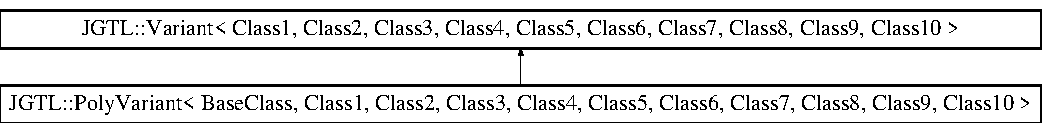
\includegraphics[height=1.64223cm]{class_j_g_t_l_1_1_poly_variant}
\end{center}
\end{figure}
\subsection*{Public Member Functions}
\begin{CompactItemize}
\item 
\hyperlink{class_j_g_t_l_1_1_poly_variant_cf2f8c79c9a93f0070cfba77cfa43d58}{Poly\-Variant} ()
\item 
Base\-Class $\ast$ \hyperlink{class_j_g_t_l_1_1_poly_variant_cee1586dc24e7836fc0cf19f9ffc5bd7}{operator $\rightarrow$ } () const
\end{CompactItemize}
\subsection*{Protected Attributes}
\begin{CompactItemize}
\item 
Base\-Class $\ast$ \hyperlink{class_j_g_t_l_1_1_poly_variant_9731a2eb9f328710229e3574e9063caa}{base}
\end{CompactItemize}
\subsubsection*{template$<$class Base\-Class, class Class1, class Class2 = Null\-Variant\-Class, class Class3 = Null\-Variant\-Class, class Class4 = Null\-Variant\-Class, class Class5 = Null\-Variant\-Class, class Class6 = Null\-Variant\-Class, class Class7 = Null\-Variant\-Class, class Class8 = Null\-Variant\-Class, class Class9 = Null\-Variant\-Class, class Class10 = Null\-Variant\-Class$>$ class JGTL::Poly\-Variant$<$ Base\-Class, Class1, Class2, Class3, Class4, Class5, Class6, Class7, Class8, Class9, Class10 $>$}



\subsection{Constructor \& Destructor Documentation}
\hypertarget{class_j_g_t_l_1_1_poly_variant_cf2f8c79c9a93f0070cfba77cfa43d58}{
\index{JGTL::PolyVariant@{JGTL::Poly\-Variant}!PolyVariant@{PolyVariant}}
\index{PolyVariant@{PolyVariant}!JGTL::PolyVariant@{JGTL::Poly\-Variant}}
\subsubsection[PolyVariant]{\setlength{\rightskip}{0pt plus 5cm}template$<$class Base\-Class, class Class1, class Class2 = Null\-Variant\-Class, class Class3 = Null\-Variant\-Class, class Class4 = Null\-Variant\-Class, class Class5 = Null\-Variant\-Class, class Class6 = Null\-Variant\-Class, class Class7 = Null\-Variant\-Class, class Class8 = Null\-Variant\-Class, class Class9 = Null\-Variant\-Class, class Class10 = Null\-Variant\-Class$>$ \hyperlink{class_j_g_t_l_1_1_poly_variant}{JGTL::Poly\-Variant}$<$ Base\-Class, Class1, Class2, Class3, Class4, Class5, Class6, Class7, Class8, Class9, Class10 $>$::\hyperlink{class_j_g_t_l_1_1_poly_variant}{Poly\-Variant} ()\hspace{0.3cm}{\tt  \mbox{[}inline\mbox{]}}}}
\label{class_j_g_t_l_1_1_poly_variant_cf2f8c79c9a93f0070cfba77cfa43d58}




\subsection{Member Function Documentation}
\hypertarget{class_j_g_t_l_1_1_poly_variant_cee1586dc24e7836fc0cf19f9ffc5bd7}{
\index{JGTL::PolyVariant@{JGTL::Poly\-Variant}!operator->@{operator-$>$}}
\index{operator->@{operator-$>$}!JGTL::PolyVariant@{JGTL::Poly\-Variant}}
\subsubsection[operator-$>$]{\setlength{\rightskip}{0pt plus 5cm}template$<$class Base\-Class, class Class1, class Class2 = Null\-Variant\-Class, class Class3 = Null\-Variant\-Class, class Class4 = Null\-Variant\-Class, class Class5 = Null\-Variant\-Class, class Class6 = Null\-Variant\-Class, class Class7 = Null\-Variant\-Class, class Class8 = Null\-Variant\-Class, class Class9 = Null\-Variant\-Class, class Class10 = Null\-Variant\-Class$>$ Base\-Class$\ast$ \hyperlink{class_j_g_t_l_1_1_poly_variant}{JGTL::Poly\-Variant}$<$ Base\-Class, Class1, Class2, Class3, Class4, Class5, Class6, Class7, Class8, Class9, Class10 $>$::operator $\rightarrow$  () const\hspace{0.3cm}{\tt  \mbox{[}inline\mbox{]}}}}
\label{class_j_g_t_l_1_1_poly_variant_cee1586dc24e7836fc0cf19f9ffc5bd7}




\subsection{Member Data Documentation}
\hypertarget{class_j_g_t_l_1_1_poly_variant_9731a2eb9f328710229e3574e9063caa}{
\index{JGTL::PolyVariant@{JGTL::Poly\-Variant}!base@{base}}
\index{base@{base}!JGTL::PolyVariant@{JGTL::Poly\-Variant}}
\subsubsection[base]{\setlength{\rightskip}{0pt plus 5cm}template$<$class Base\-Class, class Class1, class Class2 = Null\-Variant\-Class, class Class3 = Null\-Variant\-Class, class Class4 = Null\-Variant\-Class, class Class5 = Null\-Variant\-Class, class Class6 = Null\-Variant\-Class, class Class7 = Null\-Variant\-Class, class Class8 = Null\-Variant\-Class, class Class9 = Null\-Variant\-Class, class Class10 = Null\-Variant\-Class$>$ Base\-Class$\ast$ \hyperlink{class_j_g_t_l_1_1_poly_variant}{JGTL::Poly\-Variant}$<$ Base\-Class, Class1, Class2, Class3, Class4, Class5, Class6, Class7, Class8, Class9, Class10 $>$::\hyperlink{class_j_g_t_l_1_1_poly_variant_9731a2eb9f328710229e3574e9063caa}{base}\hspace{0.3cm}{\tt  \mbox{[}protected\mbox{]}}}}
\label{class_j_g_t_l_1_1_poly_variant_9731a2eb9f328710229e3574e9063caa}




The documentation for this class was generated from the following file:\begin{CompactItemize}
\item 
\hyperlink{_j_g_t_l___poly_variant_8h}{JGTL\_\-Poly\-Variant.h}\end{CompactItemize}

\hypertarget{class_j_g_t_l_1_1_pool_map}{
\section{JGTL::Pool\-Map$<$ Key, Data $>$ Class Template Reference}
\label{class_j_g_t_l_1_1_pool_map}\index{JGTL::PoolMap@{JGTL::PoolMap}}
}
{\tt \#include $<$JGTL\_\-Pool\-Map\_\-delete.h$>$}

\subsection*{Public Types}
\begin{CompactItemize}
\item 
typedef std::pair$<$ Key, Data $>$ $\ast$ \hyperlink{class_j_g_t_l_1_1_pool_map_b3af40821696ebcf9f62a3e9d91324ee}{iterator}
\item 
typedef const std::pair$<$ Key, Data $>$ $\ast$ \hyperlink{class_j_g_t_l_1_1_pool_map_123acfa775472141cec2bb3991c93d21}{const\_\-iterator}
\end{CompactItemize}
\subsection*{Public Member Functions}
\begin{CompactItemize}
\item 
\hyperlink{class_j_g_t_l_1_1_pool_map_8f488dfbc3383bc75157b60640b33ade}{Pool\-Map} (int \_\-max\-Elements)
\item 
\hyperlink{class_j_g_t_l_1_1_pool_map_a276af8c63cb02ed4d2de28bf36cd7cc}{Pool\-Map} (const \hyperlink{class_j_g_t_l_1_1_pool_map}{Pool\-Map}$<$ Key, Data $>$ \&other)
\item 
const \hyperlink{class_j_g_t_l_1_1_pool_map}{Pool\-Map} \& \hyperlink{class_j_g_t_l_1_1_pool_map_205541080219447b7651aadd391816e4}{operator=} (const \hyperlink{class_j_g_t_l_1_1_pool_map}{Pool\-Map}$<$ Key, Data $>$ \&other)
\item 
void \hyperlink{class_j_g_t_l_1_1_pool_map_3b3148e41d7f1df718801cd7396fd89f}{copy\-From} (const \hyperlink{class_j_g_t_l_1_1_pool_map}{Pool\-Map}$<$ Key, Data $>$ \&other)
\item 
virtual \hyperlink{class_j_g_t_l_1_1_pool_map_3b37f6bc0c5a42b4354edbd8ce8b907b}{$\sim$Pool\-Map} ()
\item 
void \hyperlink{class_j_g_t_l_1_1_pool_map_669bf1d78e81cdd09fb6d2b1aea4ce9a}{insert} (const Key \&key, const Data \&data)
\item 
int \hyperlink{class_j_g_t_l_1_1_pool_map_d9936165993f004d6c8b8aca4614e522}{size} ()
\item 
void \hyperlink{class_j_g_t_l_1_1_pool_map_e89e7a5f21139dd6dd927d1898bb9f7c}{clear} ()
\item 
\hyperlink{class_j_g_t_l_1_1_pool_map_b3af40821696ebcf9f62a3e9d91324ee}{iterator} \hyperlink{class_j_g_t_l_1_1_pool_map_2a375fae39774d1abe87588cffc9411a}{begin} ()
\item 
\hyperlink{class_j_g_t_l_1_1_pool_map_b3af40821696ebcf9f62a3e9d91324ee}{iterator} \hyperlink{class_j_g_t_l_1_1_pool_map_8d356ec14bedcd97fc2428ee7c7ba75b}{end} ()
\item 
const bool \hyperlink{class_j_g_t_l_1_1_pool_map_ed7f7adf472a3cb6be038adafcd1db70}{has\-Key} (const Key \&key) const 
\item 
\hyperlink{class_j_g_t_l_1_1_pool_map_b3af40821696ebcf9f62a3e9d91324ee}{iterator} \hyperlink{class_j_g_t_l_1_1_pool_map_bbf48a295265f59eb595e7695997ac14}{find} (const Key \&key)
\item 
Data $\ast$ \hyperlink{class_j_g_t_l_1_1_pool_map_097cdf2c2bae8f59db2849a7b62f82d0}{get\-Data} (const Key \&key)
\item 
const Data $\ast$ \hyperlink{class_j_g_t_l_1_1_pool_map_7b04eb59001beed06626bde7622a42d0}{get\-Data} (const Key \&key) const 
\item 
const Data \& \hyperlink{class_j_g_t_l_1_1_pool_map_27a40fef553c59284fc28621fd7515b5}{get\-Data\-Ref} (const Key \&key) const 
\item 
const Data \& \hyperlink{class_j_g_t_l_1_1_pool_map_9f6083416f0d4896c13003adb5c9b935}{get\-Index\-Data} (int index) const
\item 
const Data $\ast$ \hyperlink{class_j_g_t_l_1_1_pool_map_68006d0d7c9195990a8d24dab585ce01}{get\-Index\-Data\-Ptr} (int index) const
\end{CompactItemize}
\subsection*{Protected Attributes}
\begin{CompactItemize}
\item 
int \hyperlink{class_j_g_t_l_1_1_pool_map_973160447230898cb7e0dd73ad675879}{num\-Elements}
\item 
int \hyperlink{class_j_g_t_l_1_1_pool_map_15fff9edc5d43282b599db47bfbd31f5}{max\-Elements}
\item 
std::pair$<$ Key, Data $>$ $\ast$ \hyperlink{class_j_g_t_l_1_1_pool_map_0f8e82d573853a0b6bf943f277106f7f}{data\-List}
\end{CompactItemize}
\subsubsection*{template$<$class Key, class Data$>$ class JGTL::Pool\-Map$<$ Key, Data $>$}



\subsection{Member Typedef Documentation}
\hypertarget{class_j_g_t_l_1_1_pool_map_b3af40821696ebcf9f62a3e9d91324ee}{
\index{JGTL::PoolMap@{JGTL::Pool\-Map}!iterator@{iterator}}
\index{iterator@{iterator}!JGTL::PoolMap@{JGTL::Pool\-Map}}
\subsubsection[iterator]{\setlength{\rightskip}{0pt plus 5cm}template$<$class Key, class Data$>$ typedef std::pair$<$Key,Data$>$$\ast$ \hyperlink{class_j_g_t_l_1_1_pool_map}{JGTL::Pool\-Map}$<$ Key, Data $>$::\hyperlink{class_j_g_t_l_1_1_pool_map_b3af40821696ebcf9f62a3e9d91324ee}{iterator}}}
\label{class_j_g_t_l_1_1_pool_map_b3af40821696ebcf9f62a3e9d91324ee}


\hypertarget{class_j_g_t_l_1_1_pool_map_123acfa775472141cec2bb3991c93d21}{
\index{JGTL::PoolMap@{JGTL::Pool\-Map}!const_iterator@{const\_\-iterator}}
\index{const_iterator@{const\_\-iterator}!JGTL::PoolMap@{JGTL::Pool\-Map}}
\subsubsection[const\_\-iterator]{\setlength{\rightskip}{0pt plus 5cm}template$<$class Key, class Data$>$ typedef const std::pair$<$Key,Data$>$$\ast$ \hyperlink{class_j_g_t_l_1_1_pool_map}{JGTL::Pool\-Map}$<$ Key, Data $>$::\hyperlink{class_j_g_t_l_1_1_pool_map_123acfa775472141cec2bb3991c93d21}{const\_\-iterator}}}
\label{class_j_g_t_l_1_1_pool_map_123acfa775472141cec2bb3991c93d21}




\subsection{Constructor \& Destructor Documentation}
\hypertarget{class_j_g_t_l_1_1_pool_map_8f488dfbc3383bc75157b60640b33ade}{
\index{JGTL::PoolMap@{JGTL::Pool\-Map}!PoolMap@{PoolMap}}
\index{PoolMap@{PoolMap}!JGTL::PoolMap@{JGTL::Pool\-Map}}
\subsubsection[PoolMap]{\setlength{\rightskip}{0pt plus 5cm}template$<$class Key, class Data$>$ \hyperlink{class_j_g_t_l_1_1_pool_map}{JGTL::Pool\-Map}$<$ Key, Data $>$::\hyperlink{class_j_g_t_l_1_1_pool_map}{Pool\-Map} (int {\em \_\-max\-Elements})\hspace{0.3cm}{\tt  \mbox{[}inline\mbox{]}}}}
\label{class_j_g_t_l_1_1_pool_map_8f488dfbc3383bc75157b60640b33ade}


\hypertarget{class_j_g_t_l_1_1_pool_map_a276af8c63cb02ed4d2de28bf36cd7cc}{
\index{JGTL::PoolMap@{JGTL::Pool\-Map}!PoolMap@{PoolMap}}
\index{PoolMap@{PoolMap}!JGTL::PoolMap@{JGTL::Pool\-Map}}
\subsubsection[PoolMap]{\setlength{\rightskip}{0pt plus 5cm}template$<$class Key, class Data$>$ \hyperlink{class_j_g_t_l_1_1_pool_map}{JGTL::Pool\-Map}$<$ Key, Data $>$::\hyperlink{class_j_g_t_l_1_1_pool_map}{Pool\-Map} (const \hyperlink{class_j_g_t_l_1_1_pool_map}{Pool\-Map}$<$ Key, Data $>$ \& {\em other})\hspace{0.3cm}{\tt  \mbox{[}inline\mbox{]}}}}
\label{class_j_g_t_l_1_1_pool_map_a276af8c63cb02ed4d2de28bf36cd7cc}


\hypertarget{class_j_g_t_l_1_1_pool_map_3b37f6bc0c5a42b4354edbd8ce8b907b}{
\index{JGTL::PoolMap@{JGTL::Pool\-Map}!~PoolMap@{$\sim$PoolMap}}
\index{~PoolMap@{$\sim$PoolMap}!JGTL::PoolMap@{JGTL::Pool\-Map}}
\subsubsection[$\sim$PoolMap]{\setlength{\rightskip}{0pt plus 5cm}template$<$class Key, class Data$>$ virtual \hyperlink{class_j_g_t_l_1_1_pool_map}{JGTL::Pool\-Map}$<$ Key, Data $>$::$\sim$\hyperlink{class_j_g_t_l_1_1_pool_map}{Pool\-Map} ()\hspace{0.3cm}{\tt  \mbox{[}inline, virtual\mbox{]}}}}
\label{class_j_g_t_l_1_1_pool_map_3b37f6bc0c5a42b4354edbd8ce8b907b}




\subsection{Member Function Documentation}
\hypertarget{class_j_g_t_l_1_1_pool_map_205541080219447b7651aadd391816e4}{
\index{JGTL::PoolMap@{JGTL::Pool\-Map}!operator=@{operator=}}
\index{operator=@{operator=}!JGTL::PoolMap@{JGTL::Pool\-Map}}
\subsubsection[operator=]{\setlength{\rightskip}{0pt plus 5cm}template$<$class Key, class Data$>$ const \hyperlink{class_j_g_t_l_1_1_pool_map}{Pool\-Map}\& \hyperlink{class_j_g_t_l_1_1_pool_map}{JGTL::Pool\-Map}$<$ Key, Data $>$::operator= (const \hyperlink{class_j_g_t_l_1_1_pool_map}{Pool\-Map}$<$ Key, Data $>$ \& {\em other})\hspace{0.3cm}{\tt  \mbox{[}inline\mbox{]}}}}
\label{class_j_g_t_l_1_1_pool_map_205541080219447b7651aadd391816e4}


\hypertarget{class_j_g_t_l_1_1_pool_map_3b3148e41d7f1df718801cd7396fd89f}{
\index{JGTL::PoolMap@{JGTL::Pool\-Map}!copyFrom@{copyFrom}}
\index{copyFrom@{copyFrom}!JGTL::PoolMap@{JGTL::Pool\-Map}}
\subsubsection[copyFrom]{\setlength{\rightskip}{0pt plus 5cm}template$<$class Key, class Data$>$ void \hyperlink{class_j_g_t_l_1_1_pool_map}{JGTL::Pool\-Map}$<$ Key, Data $>$::copy\-From (const \hyperlink{class_j_g_t_l_1_1_pool_map}{Pool\-Map}$<$ Key, Data $>$ \& {\em other})\hspace{0.3cm}{\tt  \mbox{[}inline\mbox{]}}}}
\label{class_j_g_t_l_1_1_pool_map_3b3148e41d7f1df718801cd7396fd89f}


\hypertarget{class_j_g_t_l_1_1_pool_map_669bf1d78e81cdd09fb6d2b1aea4ce9a}{
\index{JGTL::PoolMap@{JGTL::Pool\-Map}!insert@{insert}}
\index{insert@{insert}!JGTL::PoolMap@{JGTL::Pool\-Map}}
\subsubsection[insert]{\setlength{\rightskip}{0pt plus 5cm}template$<$class Key, class Data$>$ void \hyperlink{class_j_g_t_l_1_1_pool_map}{JGTL::Pool\-Map}$<$ Key, Data $>$::insert (const Key \& {\em key}, const Data \& {\em data})\hspace{0.3cm}{\tt  \mbox{[}inline\mbox{]}}}}
\label{class_j_g_t_l_1_1_pool_map_669bf1d78e81cdd09fb6d2b1aea4ce9a}


\hypertarget{class_j_g_t_l_1_1_pool_map_d9936165993f004d6c8b8aca4614e522}{
\index{JGTL::PoolMap@{JGTL::Pool\-Map}!size@{size}}
\index{size@{size}!JGTL::PoolMap@{JGTL::Pool\-Map}}
\subsubsection[size]{\setlength{\rightskip}{0pt plus 5cm}template$<$class Key, class Data$>$ int \hyperlink{class_j_g_t_l_1_1_pool_map}{JGTL::Pool\-Map}$<$ Key, Data $>$::size ()\hspace{0.3cm}{\tt  \mbox{[}inline\mbox{]}}}}
\label{class_j_g_t_l_1_1_pool_map_d9936165993f004d6c8b8aca4614e522}


\hypertarget{class_j_g_t_l_1_1_pool_map_e89e7a5f21139dd6dd927d1898bb9f7c}{
\index{JGTL::PoolMap@{JGTL::Pool\-Map}!clear@{clear}}
\index{clear@{clear}!JGTL::PoolMap@{JGTL::Pool\-Map}}
\subsubsection[clear]{\setlength{\rightskip}{0pt plus 5cm}template$<$class Key, class Data$>$ void \hyperlink{class_j_g_t_l_1_1_pool_map}{JGTL::Pool\-Map}$<$ Key, Data $>$::clear ()\hspace{0.3cm}{\tt  \mbox{[}inline\mbox{]}}}}
\label{class_j_g_t_l_1_1_pool_map_e89e7a5f21139dd6dd927d1898bb9f7c}


\hypertarget{class_j_g_t_l_1_1_pool_map_2a375fae39774d1abe87588cffc9411a}{
\index{JGTL::PoolMap@{JGTL::Pool\-Map}!begin@{begin}}
\index{begin@{begin}!JGTL::PoolMap@{JGTL::Pool\-Map}}
\subsubsection[begin]{\setlength{\rightskip}{0pt plus 5cm}template$<$class Key, class Data$>$ \hyperlink{class_j_g_t_l_1_1_pool_map_b3af40821696ebcf9f62a3e9d91324ee}{iterator} \hyperlink{class_j_g_t_l_1_1_pool_map}{JGTL::Pool\-Map}$<$ Key, Data $>$::begin ()\hspace{0.3cm}{\tt  \mbox{[}inline\mbox{]}}}}
\label{class_j_g_t_l_1_1_pool_map_2a375fae39774d1abe87588cffc9411a}


\hypertarget{class_j_g_t_l_1_1_pool_map_8d356ec14bedcd97fc2428ee7c7ba75b}{
\index{JGTL::PoolMap@{JGTL::Pool\-Map}!end@{end}}
\index{end@{end}!JGTL::PoolMap@{JGTL::Pool\-Map}}
\subsubsection[end]{\setlength{\rightskip}{0pt plus 5cm}template$<$class Key, class Data$>$ \hyperlink{class_j_g_t_l_1_1_pool_map_b3af40821696ebcf9f62a3e9d91324ee}{iterator} \hyperlink{class_j_g_t_l_1_1_pool_map}{JGTL::Pool\-Map}$<$ Key, Data $>$::end ()\hspace{0.3cm}{\tt  \mbox{[}inline\mbox{]}}}}
\label{class_j_g_t_l_1_1_pool_map_8d356ec14bedcd97fc2428ee7c7ba75b}


\hypertarget{class_j_g_t_l_1_1_pool_map_ed7f7adf472a3cb6be038adafcd1db70}{
\index{JGTL::PoolMap@{JGTL::Pool\-Map}!hasKey@{hasKey}}
\index{hasKey@{hasKey}!JGTL::PoolMap@{JGTL::Pool\-Map}}
\subsubsection[hasKey]{\setlength{\rightskip}{0pt plus 5cm}template$<$class Key, class Data$>$ const bool \hyperlink{class_j_g_t_l_1_1_pool_map}{JGTL::Pool\-Map}$<$ Key, Data $>$::has\-Key (const Key \& {\em key}) const\hspace{0.3cm}{\tt  \mbox{[}inline\mbox{]}}}}
\label{class_j_g_t_l_1_1_pool_map_ed7f7adf472a3cb6be038adafcd1db70}


\hypertarget{class_j_g_t_l_1_1_pool_map_bbf48a295265f59eb595e7695997ac14}{
\index{JGTL::PoolMap@{JGTL::Pool\-Map}!find@{find}}
\index{find@{find}!JGTL::PoolMap@{JGTL::Pool\-Map}}
\subsubsection[find]{\setlength{\rightskip}{0pt plus 5cm}template$<$class Key, class Data$>$ \hyperlink{class_j_g_t_l_1_1_pool_map_b3af40821696ebcf9f62a3e9d91324ee}{iterator} \hyperlink{class_j_g_t_l_1_1_pool_map}{JGTL::Pool\-Map}$<$ Key, Data $>$::find (const Key \& {\em key})\hspace{0.3cm}{\tt  \mbox{[}inline\mbox{]}}}}
\label{class_j_g_t_l_1_1_pool_map_bbf48a295265f59eb595e7695997ac14}


\hypertarget{class_j_g_t_l_1_1_pool_map_097cdf2c2bae8f59db2849a7b62f82d0}{
\index{JGTL::PoolMap@{JGTL::Pool\-Map}!getData@{getData}}
\index{getData@{getData}!JGTL::PoolMap@{JGTL::Pool\-Map}}
\subsubsection[getData]{\setlength{\rightskip}{0pt plus 5cm}template$<$class Key, class Data$>$ Data$\ast$ \hyperlink{class_j_g_t_l_1_1_pool_map}{JGTL::Pool\-Map}$<$ Key, Data $>$::get\-Data (const Key \& {\em key})\hspace{0.3cm}{\tt  \mbox{[}inline\mbox{]}}}}
\label{class_j_g_t_l_1_1_pool_map_097cdf2c2bae8f59db2849a7b62f82d0}


\hypertarget{class_j_g_t_l_1_1_pool_map_7b04eb59001beed06626bde7622a42d0}{
\index{JGTL::PoolMap@{JGTL::Pool\-Map}!getData@{getData}}
\index{getData@{getData}!JGTL::PoolMap@{JGTL::Pool\-Map}}
\subsubsection[getData]{\setlength{\rightskip}{0pt plus 5cm}template$<$class Key, class Data$>$ const Data$\ast$ \hyperlink{class_j_g_t_l_1_1_pool_map}{JGTL::Pool\-Map}$<$ Key, Data $>$::get\-Data (const Key \& {\em key}) const\hspace{0.3cm}{\tt  \mbox{[}inline\mbox{]}}}}
\label{class_j_g_t_l_1_1_pool_map_7b04eb59001beed06626bde7622a42d0}


\hypertarget{class_j_g_t_l_1_1_pool_map_27a40fef553c59284fc28621fd7515b5}{
\index{JGTL::PoolMap@{JGTL::Pool\-Map}!getDataRef@{getDataRef}}
\index{getDataRef@{getDataRef}!JGTL::PoolMap@{JGTL::Pool\-Map}}
\subsubsection[getDataRef]{\setlength{\rightskip}{0pt plus 5cm}template$<$class Key, class Data$>$ const Data\& \hyperlink{class_j_g_t_l_1_1_pool_map}{JGTL::Pool\-Map}$<$ Key, Data $>$::get\-Data\-Ref (const Key \& {\em key}) const\hspace{0.3cm}{\tt  \mbox{[}inline\mbox{]}}}}
\label{class_j_g_t_l_1_1_pool_map_27a40fef553c59284fc28621fd7515b5}


\hypertarget{class_j_g_t_l_1_1_pool_map_9f6083416f0d4896c13003adb5c9b935}{
\index{JGTL::PoolMap@{JGTL::Pool\-Map}!getIndexData@{getIndexData}}
\index{getIndexData@{getIndexData}!JGTL::PoolMap@{JGTL::Pool\-Map}}
\subsubsection[getIndexData]{\setlength{\rightskip}{0pt plus 5cm}template$<$class Key, class Data$>$ const Data\& \hyperlink{class_j_g_t_l_1_1_pool_map}{JGTL::Pool\-Map}$<$ Key, Data $>$::get\-Index\-Data (int {\em index}) const\hspace{0.3cm}{\tt  \mbox{[}inline\mbox{]}}}}
\label{class_j_g_t_l_1_1_pool_map_9f6083416f0d4896c13003adb5c9b935}


\hypertarget{class_j_g_t_l_1_1_pool_map_68006d0d7c9195990a8d24dab585ce01}{
\index{JGTL::PoolMap@{JGTL::Pool\-Map}!getIndexDataPtr@{getIndexDataPtr}}
\index{getIndexDataPtr@{getIndexDataPtr}!JGTL::PoolMap@{JGTL::Pool\-Map}}
\subsubsection[getIndexDataPtr]{\setlength{\rightskip}{0pt plus 5cm}template$<$class Key, class Data$>$ const Data$\ast$ \hyperlink{class_j_g_t_l_1_1_pool_map}{JGTL::Pool\-Map}$<$ Key, Data $>$::get\-Index\-Data\-Ptr (int {\em index}) const\hspace{0.3cm}{\tt  \mbox{[}inline\mbox{]}}}}
\label{class_j_g_t_l_1_1_pool_map_68006d0d7c9195990a8d24dab585ce01}




\subsection{Member Data Documentation}
\hypertarget{class_j_g_t_l_1_1_pool_map_973160447230898cb7e0dd73ad675879}{
\index{JGTL::PoolMap@{JGTL::Pool\-Map}!numElements@{numElements}}
\index{numElements@{numElements}!JGTL::PoolMap@{JGTL::Pool\-Map}}
\subsubsection[numElements]{\setlength{\rightskip}{0pt plus 5cm}template$<$class Key, class Data$>$ int \hyperlink{class_j_g_t_l_1_1_pool_map}{JGTL::Pool\-Map}$<$ Key, Data $>$::\hyperlink{class_j_g_t_l_1_1_pool_map_973160447230898cb7e0dd73ad675879}{num\-Elements}\hspace{0.3cm}{\tt  \mbox{[}protected\mbox{]}}}}
\label{class_j_g_t_l_1_1_pool_map_973160447230898cb7e0dd73ad675879}


\hypertarget{class_j_g_t_l_1_1_pool_map_15fff9edc5d43282b599db47bfbd31f5}{
\index{JGTL::PoolMap@{JGTL::Pool\-Map}!maxElements@{maxElements}}
\index{maxElements@{maxElements}!JGTL::PoolMap@{JGTL::Pool\-Map}}
\subsubsection[maxElements]{\setlength{\rightskip}{0pt plus 5cm}template$<$class Key, class Data$>$ int \hyperlink{class_j_g_t_l_1_1_pool_map}{JGTL::Pool\-Map}$<$ Key, Data $>$::\hyperlink{class_j_g_t_l_1_1_pool_map_15fff9edc5d43282b599db47bfbd31f5}{max\-Elements}\hspace{0.3cm}{\tt  \mbox{[}protected\mbox{]}}}}
\label{class_j_g_t_l_1_1_pool_map_15fff9edc5d43282b599db47bfbd31f5}


\hypertarget{class_j_g_t_l_1_1_pool_map_0f8e82d573853a0b6bf943f277106f7f}{
\index{JGTL::PoolMap@{JGTL::Pool\-Map}!dataList@{dataList}}
\index{dataList@{dataList}!JGTL::PoolMap@{JGTL::Pool\-Map}}
\subsubsection[dataList]{\setlength{\rightskip}{0pt plus 5cm}template$<$class Key, class Data$>$ std::pair$<$Key,Data$>$$\ast$ \hyperlink{class_j_g_t_l_1_1_pool_map}{JGTL::Pool\-Map}$<$ Key, Data $>$::\hyperlink{class_j_g_t_l_1_1_pool_map_0f8e82d573853a0b6bf943f277106f7f}{data\-List}\hspace{0.3cm}{\tt  \mbox{[}protected\mbox{]}}}}
\label{class_j_g_t_l_1_1_pool_map_0f8e82d573853a0b6bf943f277106f7f}




The documentation for this class was generated from the following file:\begin{CompactItemize}
\item 
\hyperlink{_j_g_t_l___pool_map__delete_8h}{JGTL\_\-Pool\-Map\_\-delete.h}\end{CompactItemize}

\hypertarget{struct_j_g_t_l_1_1_profile_block}{
\section{JGTL::Profile\-Block Struct Reference}
\label{struct_j_g_t_l_1_1_profile_block}\index{JGTL::ProfileBlock@{JGTL::ProfileBlock}}
}
{\tt \#include $<$JGTL\_\-Quick\-Prof.h$>$}

\subsection*{Public Member Functions}
\begin{CompactItemize}
\item 
\hyperlink{struct_j_g_t_l_1_1_profile_block_978acff6a004461d28e440472dd5d895}{Profile\-Block} ()
\end{CompactItemize}
\subsection*{Public Attributes}
\begin{CompactItemize}
\item 
unsigned long int \hyperlink{struct_j_g_t_l_1_1_profile_block_49aa3dc0ecd58718ecccdb23ff8ca4f5}{current\-Block\-Start\-Microseconds}
\begin{CompactList}\small\item\em The starting time (in us) of the current block update. \item\end{CompactList}\item 
unsigned long int \hyperlink{struct_j_g_t_l_1_1_profile_block_4dbffcbbb50e7e6affc6116f361a2417}{current\-Cycle\-Total\-Microseconds}
\item 
double \hyperlink{struct_j_g_t_l_1_1_profile_block_d995e3d70a098db440f9002aef727d40}{avg\-Cycle\-Total\-Microseconds}
\item 
unsigned long int \hyperlink{struct_j_g_t_l_1_1_profile_block_457aeecf869359baed544fa467d46b42}{total\-Microseconds}
\begin{CompactList}\small\item\em The total accumulated time (in us) spent in this block. \item\end{CompactList}\item 
unsigned long int \hyperlink{struct_j_g_t_l_1_1_profile_block_8edab8046fbb65df2c8bef07c638829b}{smallest\-Cycle\-Microseconds}
\begin{CompactList}\small\item\em The best time for this block. \item\end{CompactList}\item 
double \hyperlink{struct_j_g_t_l_1_1_profile_block_75a7c8c6d211c681097adf60c797c56e}{smallest\-Cycle\-Percent}
\item 
unsigned long int \hyperlink{struct_j_g_t_l_1_1_profile_block_6dc09e684472a23ea795a39d3c113977}{largest\-Cycle\-Microseconds}
\begin{CompactList}\small\item\em The worst time for this block. \item\end{CompactList}\item 
double \hyperlink{struct_j_g_t_l_1_1_profile_block_15d4a484adfda90c368bbacdf680d99c}{largest\-Cycle\-Percent}
\end{CompactItemize}


\subsection{Detailed Description}
A simple data structure representing a single timed block of code. 



\subsection{Constructor \& Destructor Documentation}
\hypertarget{struct_j_g_t_l_1_1_profile_block_978acff6a004461d28e440472dd5d895}{
\index{JGTL::ProfileBlock@{JGTL::Profile\-Block}!ProfileBlock@{ProfileBlock}}
\index{ProfileBlock@{ProfileBlock}!JGTL::ProfileBlock@{JGTL::Profile\-Block}}
\subsubsection[ProfileBlock]{\setlength{\rightskip}{0pt plus 5cm}JGTL::Profile\-Block::Profile\-Block ()\hspace{0.3cm}{\tt  \mbox{[}inline\mbox{]}}}}
\label{struct_j_g_t_l_1_1_profile_block_978acff6a004461d28e440472dd5d895}




\subsection{Member Data Documentation}
\hypertarget{struct_j_g_t_l_1_1_profile_block_49aa3dc0ecd58718ecccdb23ff8ca4f5}{
\index{JGTL::ProfileBlock@{JGTL::Profile\-Block}!currentBlockStartMicroseconds@{currentBlockStartMicroseconds}}
\index{currentBlockStartMicroseconds@{currentBlockStartMicroseconds}!JGTL::ProfileBlock@{JGTL::Profile\-Block}}
\subsubsection[currentBlockStartMicroseconds]{\setlength{\rightskip}{0pt plus 5cm}unsigned long int \hyperlink{struct_j_g_t_l_1_1_profile_block_49aa3dc0ecd58718ecccdb23ff8ca4f5}{JGTL::Profile\-Block::current\-Block\-Start\-Microseconds}}}
\label{struct_j_g_t_l_1_1_profile_block_49aa3dc0ecd58718ecccdb23ff8ca4f5}


The starting time (in us) of the current block update. 

\hypertarget{struct_j_g_t_l_1_1_profile_block_4dbffcbbb50e7e6affc6116f361a2417}{
\index{JGTL::ProfileBlock@{JGTL::Profile\-Block}!currentCycleTotalMicroseconds@{currentCycleTotalMicroseconds}}
\index{currentCycleTotalMicroseconds@{currentCycleTotalMicroseconds}!JGTL::ProfileBlock@{JGTL::Profile\-Block}}
\subsubsection[currentCycleTotalMicroseconds]{\setlength{\rightskip}{0pt plus 5cm}unsigned long int \hyperlink{struct_j_g_t_l_1_1_profile_block_4dbffcbbb50e7e6affc6116f361a2417}{JGTL::Profile\-Block::current\-Cycle\-Total\-Microseconds}}}
\label{struct_j_g_t_l_1_1_profile_block_4dbffcbbb50e7e6affc6116f361a2417}


The accumulated time (in us) spent in this block during the current profiling cycle. \hypertarget{struct_j_g_t_l_1_1_profile_block_d995e3d70a098db440f9002aef727d40}{
\index{JGTL::ProfileBlock@{JGTL::Profile\-Block}!avgCycleTotalMicroseconds@{avgCycleTotalMicroseconds}}
\index{avgCycleTotalMicroseconds@{avgCycleTotalMicroseconds}!JGTL::ProfileBlock@{JGTL::Profile\-Block}}
\subsubsection[avgCycleTotalMicroseconds]{\setlength{\rightskip}{0pt plus 5cm}double \hyperlink{struct_j_g_t_l_1_1_profile_block_d995e3d70a098db440f9002aef727d40}{JGTL::Profile\-Block::avg\-Cycle\-Total\-Microseconds}}}
\label{struct_j_g_t_l_1_1_profile_block_d995e3d70a098db440f9002aef727d40}


The accumulated time (in us) spent in this block during the past profiling cycle. \hypertarget{struct_j_g_t_l_1_1_profile_block_457aeecf869359baed544fa467d46b42}{
\index{JGTL::ProfileBlock@{JGTL::Profile\-Block}!totalMicroseconds@{totalMicroseconds}}
\index{totalMicroseconds@{totalMicroseconds}!JGTL::ProfileBlock@{JGTL::Profile\-Block}}
\subsubsection[totalMicroseconds]{\setlength{\rightskip}{0pt plus 5cm}unsigned long int \hyperlink{struct_j_g_t_l_1_1_profile_block_457aeecf869359baed544fa467d46b42}{JGTL::Profile\-Block::total\-Microseconds}}}
\label{struct_j_g_t_l_1_1_profile_block_457aeecf869359baed544fa467d46b42}


The total accumulated time (in us) spent in this block. 

\hypertarget{struct_j_g_t_l_1_1_profile_block_8edab8046fbb65df2c8bef07c638829b}{
\index{JGTL::ProfileBlock@{JGTL::Profile\-Block}!smallestCycleMicroseconds@{smallestCycleMicroseconds}}
\index{smallestCycleMicroseconds@{smallestCycleMicroseconds}!JGTL::ProfileBlock@{JGTL::Profile\-Block}}
\subsubsection[smallestCycleMicroseconds]{\setlength{\rightskip}{0pt plus 5cm}unsigned long int \hyperlink{struct_j_g_t_l_1_1_profile_block_8edab8046fbb65df2c8bef07c638829b}{JGTL::Profile\-Block::smallest\-Cycle\-Microseconds}}}
\label{struct_j_g_t_l_1_1_profile_block_8edab8046fbb65df2c8bef07c638829b}


The best time for this block. 

\hypertarget{struct_j_g_t_l_1_1_profile_block_75a7c8c6d211c681097adf60c797c56e}{
\index{JGTL::ProfileBlock@{JGTL::Profile\-Block}!smallestCyclePercent@{smallestCyclePercent}}
\index{smallestCyclePercent@{smallestCyclePercent}!JGTL::ProfileBlock@{JGTL::Profile\-Block}}
\subsubsection[smallestCyclePercent]{\setlength{\rightskip}{0pt plus 5cm}double \hyperlink{struct_j_g_t_l_1_1_profile_block_75a7c8c6d211c681097adf60c797c56e}{JGTL::Profile\-Block::smallest\-Cycle\-Percent}}}
\label{struct_j_g_t_l_1_1_profile_block_75a7c8c6d211c681097adf60c797c56e}


\hypertarget{struct_j_g_t_l_1_1_profile_block_6dc09e684472a23ea795a39d3c113977}{
\index{JGTL::ProfileBlock@{JGTL::Profile\-Block}!largestCycleMicroseconds@{largestCycleMicroseconds}}
\index{largestCycleMicroseconds@{largestCycleMicroseconds}!JGTL::ProfileBlock@{JGTL::Profile\-Block}}
\subsubsection[largestCycleMicroseconds]{\setlength{\rightskip}{0pt plus 5cm}unsigned long int \hyperlink{struct_j_g_t_l_1_1_profile_block_6dc09e684472a23ea795a39d3c113977}{JGTL::Profile\-Block::largest\-Cycle\-Microseconds}}}
\label{struct_j_g_t_l_1_1_profile_block_6dc09e684472a23ea795a39d3c113977}


The worst time for this block. 

\hypertarget{struct_j_g_t_l_1_1_profile_block_15d4a484adfda90c368bbacdf680d99c}{
\index{JGTL::ProfileBlock@{JGTL::Profile\-Block}!largestCyclePercent@{largestCyclePercent}}
\index{largestCyclePercent@{largestCyclePercent}!JGTL::ProfileBlock@{JGTL::Profile\-Block}}
\subsubsection[largestCyclePercent]{\setlength{\rightskip}{0pt plus 5cm}double \hyperlink{struct_j_g_t_l_1_1_profile_block_15d4a484adfda90c368bbacdf680d99c}{JGTL::Profile\-Block::largest\-Cycle\-Percent}}}
\label{struct_j_g_t_l_1_1_profile_block_15d4a484adfda90c368bbacdf680d99c}




The documentation for this struct was generated from the following file:\begin{CompactItemize}
\item 
\hyperlink{_j_g_t_l___quick_prof_8h}{JGTL\_\-Quick\-Prof.h}\end{CompactItemize}

\hypertarget{class_j_g_t_l_1_1_profile_block_handler}{
\section{JGTL::Profile\-Block\-Handler Class Reference}
\label{class_j_g_t_l_1_1_profile_block_handler}\index{JGTL::ProfileBlockHandler@{JGTL::ProfileBlockHandler}}
}
{\tt \#include $<$JGTL\_\-Quick\-Prof.h$>$}

\subsection*{Public Member Functions}
\begin{CompactItemize}
\item 
\hyperlink{class_j_g_t_l_1_1_profile_block_handler_0be8016df83b78fa35c7e31d21fc14e7}{Profile\-Block\-Handler} (const char $\ast$\_\-block\-Name)
\item 
\hyperlink{class_j_g_t_l_1_1_profile_block_handler_f34ae362cae1c68367c1221a088ef71f}{$\sim$Profile\-Block\-Handler} ()
\end{CompactItemize}
\subsection*{Protected Attributes}
\begin{CompactItemize}
\item 
const char $\ast$ \hyperlink{class_j_g_t_l_1_1_profile_block_handler_b6f85efe1308fbe8c802c26411fb28f2}{block\-Name}
\end{CompactItemize}


\subsection{Constructor \& Destructor Documentation}
\hypertarget{class_j_g_t_l_1_1_profile_block_handler_0be8016df83b78fa35c7e31d21fc14e7}{
\index{JGTL::ProfileBlockHandler@{JGTL::Profile\-Block\-Handler}!ProfileBlockHandler@{ProfileBlockHandler}}
\index{ProfileBlockHandler@{ProfileBlockHandler}!JGTL::ProfileBlockHandler@{JGTL::Profile\-Block\-Handler}}
\subsubsection[ProfileBlockHandler]{\setlength{\rightskip}{0pt plus 5cm}JGTL::Profile\-Block\-Handler::Profile\-Block\-Handler (const char $\ast$ {\em \_\-block\-Name})\hspace{0.3cm}{\tt  \mbox{[}inline\mbox{]}}}}
\label{class_j_g_t_l_1_1_profile_block_handler_0be8016df83b78fa35c7e31d21fc14e7}


\hypertarget{class_j_g_t_l_1_1_profile_block_handler_f34ae362cae1c68367c1221a088ef71f}{
\index{JGTL::ProfileBlockHandler@{JGTL::Profile\-Block\-Handler}!~ProfileBlockHandler@{$\sim$ProfileBlockHandler}}
\index{~ProfileBlockHandler@{$\sim$ProfileBlockHandler}!JGTL::ProfileBlockHandler@{JGTL::Profile\-Block\-Handler}}
\subsubsection[$\sim$ProfileBlockHandler]{\setlength{\rightskip}{0pt plus 5cm}JGTL::Profile\-Block\-Handler::$\sim$Profile\-Block\-Handler ()\hspace{0.3cm}{\tt  \mbox{[}inline\mbox{]}}}}
\label{class_j_g_t_l_1_1_profile_block_handler_f34ae362cae1c68367c1221a088ef71f}




\subsection{Member Data Documentation}
\hypertarget{class_j_g_t_l_1_1_profile_block_handler_b6f85efe1308fbe8c802c26411fb28f2}{
\index{JGTL::ProfileBlockHandler@{JGTL::Profile\-Block\-Handler}!blockName@{blockName}}
\index{blockName@{blockName}!JGTL::ProfileBlockHandler@{JGTL::Profile\-Block\-Handler}}
\subsubsection[blockName]{\setlength{\rightskip}{0pt plus 5cm}const char$\ast$ \hyperlink{class_j_g_t_l_1_1_profile_block_handler_b6f85efe1308fbe8c802c26411fb28f2}{JGTL::Profile\-Block\-Handler::block\-Name}\hspace{0.3cm}{\tt  \mbox{[}protected\mbox{]}}}}
\label{class_j_g_t_l_1_1_profile_block_handler_b6f85efe1308fbe8c802c26411fb28f2}




The documentation for this class was generated from the following file:\begin{CompactItemize}
\item 
\hyperlink{_j_g_t_l___quick_prof_8h}{JGTL\_\-Quick\-Prof.h}\end{CompactItemize}

\hypertarget{class_j_g_t_l_1_1_profiler}{
\section{JGTL::Profiler Class Reference}
\label{class_j_g_t_l_1_1_profiler}\index{JGTL::Profiler@{JGTL::Profiler}}
}
A singleton class that manages timing for a set of profiling blocks.  


{\tt \#include $<$JGTL\_\-Quick\-Prof.h$>$}

Inheritance diagram for JGTL::Profiler::\begin{figure}[H]
\begin{center}
\leavevmode
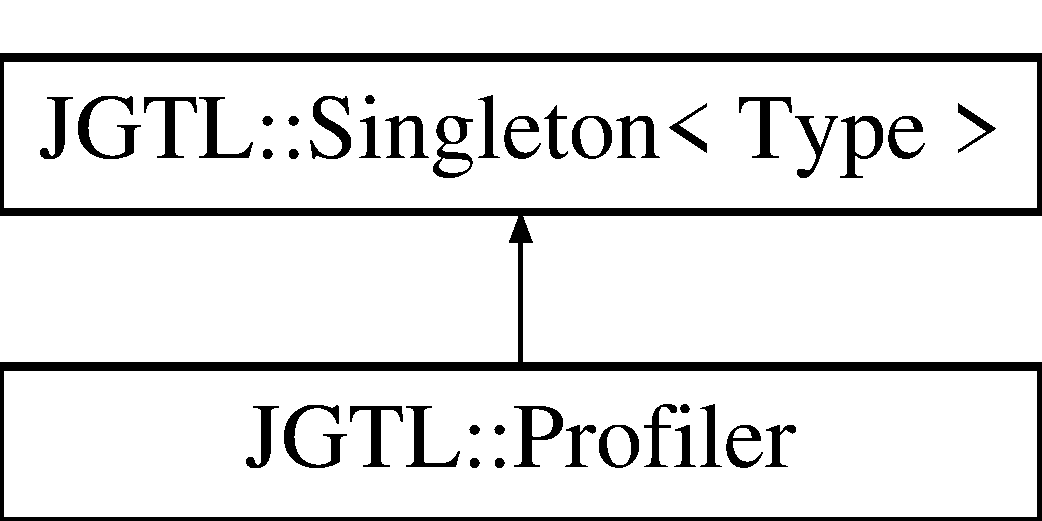
\includegraphics[height=2cm]{class_j_g_t_l_1_1_profiler}
\end{center}
\end{figure}
\subsection*{Public Member Functions}
\begin{CompactItemize}
\item 
void \hyperlink{class_j_g_t_l_1_1_profiler_6e7e7821f35ebd21a067e6ef133e367f}{init} (double smoothing=0.0, const std::string output\-Filename=\char`\"{}\char`\"{}, size\_\-t print\-Period=1, \hyperlink{namespace_j_g_t_l_11a34d88ecadd1c99354adc21fd5abe6}{Time\-Format} print\-Format=MILLISECONDS)
\item 
void \hyperlink{class_j_g_t_l_1_1_profiler_452c2c61daaec460f716b014062287d3}{reset} ()
\item 
void \hyperlink{class_j_g_t_l_1_1_profiler_c77059c32d833a4b638468b88c5dc001}{begin\-Block} (const std::string \&name)
\item 
void \hyperlink{class_j_g_t_l_1_1_profiler_42b4439144f39ab3c2f98ca9145aa99c}{end\-Block} (const std::string \&name)
\item 
void \hyperlink{class_j_g_t_l_1_1_profiler_60a7112d1d40528d3270b25b9c0967c9}{begin\-Cycle} ()
\item 
void \hyperlink{class_j_g_t_l_1_1_profiler_554c28fd5bcb0f181e05b835d3384807}{end\-Cycle} ()
\item 
double \hyperlink{class_j_g_t_l_1_1_profiler_a9e80cbb87225309047515205386270a}{get\-Avg\-Duration} (const std::string \&name, \hyperlink{namespace_j_g_t_l_11a34d88ecadd1c99354adc21fd5abe6}{Time\-Format} format)
\item 
std::string \hyperlink{class_j_g_t_l_1_1_profiler_b168b01e49b5ec112e13a1673ee56fd9}{get\-Summary} (\hyperlink{namespace_j_g_t_l_11a34d88ecadd1c99354adc21fd5abe6}{Time\-Format} format=PERCENT)
\end{CompactItemize}
\subsection*{Static Public Member Functions}
\begin{CompactItemize}
\item 
static \hyperlink{class_j_g_t_l_1_1_profiler}{Profiler} $\ast$ \hyperlink{class_j_g_t_l_1_1_profiler_a88c187ec0ec5d886eb0fb6bee98b7e5}{create\-Instance} ()
\item 
static void \hyperlink{class_j_g_t_l_1_1_profiler_cb990d68355312b6cd7a1f494e4dd33c}{destroy\-Instance} ()
\end{CompactItemize}
\subsection*{Protected Member Functions}
\begin{CompactItemize}
\item 
\hyperlink{class_j_g_t_l_1_1_profiler_8e373e2c712a2828e5384e9079958f9f}{Profiler} ()
\item 
virtual \hyperlink{class_j_g_t_l_1_1_profiler_d3678f506e4d2342604423fa035930be}{$\sim$Profiler} ()
\item 
void \hyperlink{class_j_g_t_l_1_1_profiler_d246ea0daca1f81252ff2bd316ea6d08}{print\-Error} (const std::string \&msg)
\item 
\hyperlink{struct_j_g_t_l_1_1_profile_block}{Profile\-Block} $\ast$ \hyperlink{class_j_g_t_l_1_1_profiler_cfa347cb9cc960c9c4fdf0d886785153}{get\-Profile\-Block} (const std::string \&name)
\item 
double \hyperlink{class_j_g_t_l_1_1_profiler_ee7211e4dc27568848d92ed6a66d91f9}{get\-Block\-Min\-Time} (const std::string \&name, \hyperlink{namespace_j_g_t_l_11a34d88ecadd1c99354adc21fd5abe6}{Time\-Format} format)
\item 
double \hyperlink{class_j_g_t_l_1_1_profiler_9ebb538c444e9e2069d46dd100a156d4}{get\-Block\-Total\-Time} (const std::string \&name, \hyperlink{namespace_j_g_t_l_11a34d88ecadd1c99354adc21fd5abe6}{Time\-Format} format)
\item 
double \hyperlink{class_j_g_t_l_1_1_profiler_b52d3f1a17f0e589cb898dd28b4b6f08}{get\-Block\-Max\-Time} (const std::string \&name, \hyperlink{namespace_j_g_t_l_11a34d88ecadd1c99354adc21fd5abe6}{Time\-Format} format)
\item 
double \hyperlink{class_j_g_t_l_1_1_profiler_dbdbbaa2a9a1590cbcd1f2b5204d27f1}{get\-Microseconds\-Since\-Init} ()
\item 
std::string \hyperlink{class_j_g_t_l_1_1_profiler_5aeaccffe46b7a899b57e0e54f9ce797}{get\-Suffix\-String} (\hyperlink{namespace_j_g_t_l_11a34d88ecadd1c99354adc21fd5abe6}{Time\-Format} format)
\end{CompactItemize}
\subsection*{Protected Attributes}
\begin{CompactItemize}
\item 
bool \hyperlink{class_j_g_t_l_1_1_profiler_3eb8fff02ac8b0a76273ee80486ec7cc}{m\-Enabled}
\begin{CompactList}\small\item\em Determines whether the profiler is enabled. \item\end{CompactList}\item 
\hyperlink{class_j_g_t_l_1_1_clock}{Clock} \hyperlink{class_j_g_t_l_1_1_profiler_a3e9ba84db33b2174fe49fc1d7b4939e}{m\-Clock}
\begin{CompactList}\small\item\em The clock used to time profile blocks. \item\end{CompactList}\item 
unsigned long int \hyperlink{class_j_g_t_l_1_1_profiler_c68abd2b4577f814f6f42e1f7a91cc88}{m\-Current\-Cycle\-Start\-Microseconds}
\begin{CompactList}\small\item\em The starting time (in us) of the current profiling cycle. \item\end{CompactList}\item 
unsigned long int \hyperlink{class_j_g_t_l_1_1_profiler_e6bcfdec9aa0d82a91c3c5b7f4338613}{m\-Last\-Cycle\-Duration\-Microseconds}
\begin{CompactList}\small\item\em The duration (in us) of the most recent profiling cycle. \item\end{CompactList}\item 
\hyperlink{class_j_g_t_l_1_1_dynamic_pool_map}{Dynamic\-Pool\-Map}$<$ std::string, \hyperlink{struct_j_g_t_l_1_1_profile_block}{Profile\-Block} $\ast$ $>$ \hyperlink{class_j_g_t_l_1_1_profiler_7ac2afca08882c6e136cf31d614e1617}{m\-Profile\-Blocks}
\begin{CompactList}\small\item\em Internal map of named profile blocks. \item\end{CompactList}\item 
std::ofstream \hyperlink{class_j_g_t_l_1_1_profiler_23216cd9e785ee8617fbe6d6c15008f0}{m\-Output\-File}
\begin{CompactList}\small\item\em The data output file used if this feature is enabled in init. \item\end{CompactList}\item 
bool \hyperlink{class_j_g_t_l_1_1_profiler_e5c5d7ecb757126d6085e3b2eacbb144}{m\-First\-File\-Output}
\begin{CompactList}\small\item\em Tracks whether we have begun printing data to the output file. \item\end{CompactList}\item 
double \hyperlink{class_j_g_t_l_1_1_profiler_00cadccfc6c462cc084e827b69794363}{m\-Moving\-Avg\-Scalar}
\item 
size\_\-t \hyperlink{class_j_g_t_l_1_1_profiler_de2b79bbd0a6845cf50a47435cb5265b}{m\-Print\-Period}
\item 
\hyperlink{namespace_j_g_t_l_11a34d88ecadd1c99354adc21fd5abe6}{Time\-Format} \hyperlink{class_j_g_t_l_1_1_profiler_98b7dbee91f283a2f2a958e9f0acc4c4}{m\-Print\-Format}
\begin{CompactList}\small\item\em The time format used when printing timing data to the output file. \item\end{CompactList}\item 
size\_\-t \hyperlink{class_j_g_t_l_1_1_profiler_77a79635f96581b9038410277fb1be34}{m\-Cycle\-Counter}
\begin{CompactList}\small\item\em Keeps track of how many cycles have elapsed (for printing). \item\end{CompactList}\item 
bool \hyperlink{class_j_g_t_l_1_1_profiler_32a05ea51b894c089796b6fa0e5d2aa9}{m\-First\-Cycle}
\begin{CompactList}\small\item\em Used to update the initial average cycle times. \item\end{CompactList}\item 
unsigned long \hyperlink{class_j_g_t_l_1_1_profiler_c85e5809a50c45b86ac345af710da5c3}{microseconds\-Since\-Init}
\end{CompactItemize}


\subsection{Detailed Description}
A singleton class that manages timing for a set of profiling blocks. 



\subsection{Constructor \& Destructor Documentation}
\hypertarget{class_j_g_t_l_1_1_profiler_8e373e2c712a2828e5384e9079958f9f}{
\index{JGTL::Profiler@{JGTL::Profiler}!Profiler@{Profiler}}
\index{Profiler@{Profiler}!JGTL::Profiler@{JGTL::Profiler}}
\subsubsection[Profiler]{\setlength{\rightskip}{0pt plus 5cm}JGTL::Profiler::Profiler ()\hspace{0.3cm}{\tt  \mbox{[}inline, protected\mbox{]}}}}
\label{class_j_g_t_l_1_1_profiler_8e373e2c712a2828e5384e9079958f9f}


\hypertarget{class_j_g_t_l_1_1_profiler_d3678f506e4d2342604423fa035930be}{
\index{JGTL::Profiler@{JGTL::Profiler}!~Profiler@{$\sim$Profiler}}
\index{~Profiler@{$\sim$Profiler}!JGTL::Profiler@{JGTL::Profiler}}
\subsubsection[$\sim$Profiler]{\setlength{\rightskip}{0pt plus 5cm}JGTL::Profiler::$\sim$Profiler ()\hspace{0.3cm}{\tt  \mbox{[}inline, protected, virtual\mbox{]}}}}
\label{class_j_g_t_l_1_1_profiler_d3678f506e4d2342604423fa035930be}




\subsection{Member Function Documentation}
\hypertarget{class_j_g_t_l_1_1_profiler_a88c187ec0ec5d886eb0fb6bee98b7e5}{
\index{JGTL::Profiler@{JGTL::Profiler}!createInstance@{createInstance}}
\index{createInstance@{createInstance}!JGTL::Profiler@{JGTL::Profiler}}
\subsubsection[createInstance]{\setlength{\rightskip}{0pt plus 5cm}static \hyperlink{class_j_g_t_l_1_1_profiler}{Profiler}$\ast$ JGTL::Profiler::create\-Instance ()\hspace{0.3cm}{\tt  \mbox{[}inline, static\mbox{]}}}}
\label{class_j_g_t_l_1_1_profiler_a88c187ec0ec5d886eb0fb6bee98b7e5}


\hypertarget{class_j_g_t_l_1_1_profiler_cb990d68355312b6cd7a1f494e4dd33c}{
\index{JGTL::Profiler@{JGTL::Profiler}!destroyInstance@{destroyInstance}}
\index{destroyInstance@{destroyInstance}!JGTL::Profiler@{JGTL::Profiler}}
\subsubsection[destroyInstance]{\setlength{\rightskip}{0pt plus 5cm}static void JGTL::Profiler::destroy\-Instance ()\hspace{0.3cm}{\tt  \mbox{[}inline, static\mbox{]}}}}
\label{class_j_g_t_l_1_1_profiler_cb990d68355312b6cd7a1f494e4dd33c}




Reimplemented from \hyperlink{class_j_g_t_l_1_1_singleton_59788c79ef7102b584b475aafc9e2315}{JGTL::Singleton$<$ Type $>$}.\hypertarget{class_j_g_t_l_1_1_profiler_6e7e7821f35ebd21a067e6ef133e367f}{
\index{JGTL::Profiler@{JGTL::Profiler}!init@{init}}
\index{init@{init}!JGTL::Profiler@{JGTL::Profiler}}
\subsubsection[init]{\setlength{\rightskip}{0pt plus 5cm}void JGTL::Profiler::init (double {\em smoothing} = {\tt 0.0}, const std::string {\em output\-Filename} = {\tt \char`\"{}\char`\"{}}, size\_\-t {\em print\-Period} = {\tt 1}, \hyperlink{namespace_j_g_t_l_11a34d88ecadd1c99354adc21fd5abe6}{Time\-Format} {\em print\-Format} = {\tt MILLISECONDS})\hspace{0.3cm}{\tt  \mbox{[}inline\mbox{]}}}}
\label{class_j_g_t_l_1_1_profiler_6e7e7821f35ebd21a067e6ef133e367f}


Initializes the profiler.

This must be called first. If this is never called, the profiler is effectively disabled, and all other functions will return immediately.

\begin{Desc}
\item[Parameters:]
\begin{description}
\item[{\em smoothing}]The measured duration for each profile block can be averaged across multiple cycles, and this parameter defines the smoothness of this averaging process. The higher the value, the smoother the resulting average durations will appear. Leaving it at zero will essentially disable the smoothing effect. More specifically, this parameter is a time constant (defined in terms of cycles) that defines an exponentially-weighted moving average. For example, a value of 4.0 means the past four cycles will contribute 63\% of the current weighted average. This value must be $>$= 0. \item[{\em output\-Filename}]If defined, enables timing data to be printed to a data file for later analysis. \item[{\em print\-Period}]Defines how often data is printed to the file, in number of profiling cycles. For example, set this to 1 if you want data printed after each cycle, or 5 if you want it printed every 5 cycles. It is a good idea to increase this if you don't want huge data files. Keep in mind, however, that when you increase this, you might want to increase the smoothing parameter. (A good heuristic is to set the smoothing parameter equal to the print period.) This value must be $>$= 1. \item[{\em print\-Format}]Defines the format used when printing data to a file. \end{description}
\end{Desc}
\hypertarget{class_j_g_t_l_1_1_profiler_452c2c61daaec460f716b014062287d3}{
\index{JGTL::Profiler@{JGTL::Profiler}!reset@{reset}}
\index{reset@{reset}!JGTL::Profiler@{JGTL::Profiler}}
\subsubsection[reset]{\setlength{\rightskip}{0pt plus 5cm}void JGTL::Profiler::reset ()\hspace{0.3cm}{\tt  \mbox{[}inline\mbox{]}}}}
\label{class_j_g_t_l_1_1_profiler_452c2c61daaec460f716b014062287d3}


\hypertarget{class_j_g_t_l_1_1_profiler_c77059c32d833a4b638468b88c5dc001}{
\index{JGTL::Profiler@{JGTL::Profiler}!beginBlock@{beginBlock}}
\index{beginBlock@{beginBlock}!JGTL::Profiler@{JGTL::Profiler}}
\subsubsection[beginBlock]{\setlength{\rightskip}{0pt plus 5cm}void JGTL::Profiler::begin\-Block (const std::string \& {\em name})\hspace{0.3cm}{\tt  \mbox{[}inline\mbox{]}}}}
\label{class_j_g_t_l_1_1_profiler_c77059c32d833a4b638468b88c5dc001}


Begins timing the named block of code.

\begin{Desc}
\item[Parameters:]
\begin{description}
\item[{\em name}]The name of the block. \end{description}
\end{Desc}
\hypertarget{class_j_g_t_l_1_1_profiler_42b4439144f39ab3c2f98ca9145aa99c}{
\index{JGTL::Profiler@{JGTL::Profiler}!endBlock@{endBlock}}
\index{endBlock@{endBlock}!JGTL::Profiler@{JGTL::Profiler}}
\subsubsection[endBlock]{\setlength{\rightskip}{0pt plus 5cm}void JGTL::Profiler::end\-Block (const std::string \& {\em name})\hspace{0.3cm}{\tt  \mbox{[}inline\mbox{]}}}}
\label{class_j_g_t_l_1_1_profiler_42b4439144f39ab3c2f98ca9145aa99c}


Defines the end of the named timing block.

\begin{Desc}
\item[Parameters:]
\begin{description}
\item[{\em name}]The name of the block. \end{description}
\end{Desc}
\hypertarget{class_j_g_t_l_1_1_profiler_60a7112d1d40528d3270b25b9c0967c9}{
\index{JGTL::Profiler@{JGTL::Profiler}!beginCycle@{beginCycle}}
\index{beginCycle@{beginCycle}!JGTL::Profiler@{JGTL::Profiler}}
\subsubsection[beginCycle]{\setlength{\rightskip}{0pt plus 5cm}void JGTL::Profiler::begin\-Cycle ()\hspace{0.3cm}{\tt  \mbox{[}inline\mbox{]}}}}
\label{class_j_g_t_l_1_1_profiler_60a7112d1d40528d3270b25b9c0967c9}


\hypertarget{class_j_g_t_l_1_1_profiler_554c28fd5bcb0f181e05b835d3384807}{
\index{JGTL::Profiler@{JGTL::Profiler}!endCycle@{endCycle}}
\index{endCycle@{endCycle}!JGTL::Profiler@{JGTL::Profiler}}
\subsubsection[endCycle]{\setlength{\rightskip}{0pt plus 5cm}void JGTL::Profiler::end\-Cycle ()\hspace{0.3cm}{\tt  \mbox{[}inline\mbox{]}}}}
\label{class_j_g_t_l_1_1_profiler_554c28fd5bcb0f181e05b835d3384807}


Defines the end of a profiling cycle.

Use this regularly by calling it at the end of all timing blocks. This is necessary for smoothing and for file output, but not if you just want a total summary at the end of execution (i.e. from get\-Summary). This must not be called within a timing block. \hypertarget{class_j_g_t_l_1_1_profiler_a9e80cbb87225309047515205386270a}{
\index{JGTL::Profiler@{JGTL::Profiler}!getAvgDuration@{getAvgDuration}}
\index{getAvgDuration@{getAvgDuration}!JGTL::Profiler@{JGTL::Profiler}}
\subsubsection[getAvgDuration]{\setlength{\rightskip}{0pt plus 5cm}double JGTL::Profiler::get\-Avg\-Duration (const std::string \& {\em name}, \hyperlink{namespace_j_g_t_l_11a34d88ecadd1c99354adc21fd5abe6}{Time\-Format} {\em format})\hspace{0.3cm}{\tt  \mbox{[}inline\mbox{]}}}}
\label{class_j_g_t_l_1_1_profiler_a9e80cbb87225309047515205386270a}


Returns the average time used in the named block per profiling cycle.

If smoothing is disabled (see init), this returns the most recent duration measurement.

\begin{Desc}
\item[Parameters:]
\begin{description}
\item[{\em name}]The name of the block. \item[{\em format}]The desired time format to use for the result. \end{description}
\end{Desc}
\begin{Desc}
\item[Returns:]The block's average duration per cycle. \end{Desc}
\hypertarget{class_j_g_t_l_1_1_profiler_b168b01e49b5ec112e13a1673ee56fd9}{
\index{JGTL::Profiler@{JGTL::Profiler}!getSummary@{getSummary}}
\index{getSummary@{getSummary}!JGTL::Profiler@{JGTL::Profiler}}
\subsubsection[getSummary]{\setlength{\rightskip}{0pt plus 5cm}std::string JGTL::Profiler::get\-Summary (\hyperlink{namespace_j_g_t_l_11a34d88ecadd1c99354adc21fd5abe6}{Time\-Format} {\em format} = {\tt PERCENT})\hspace{0.3cm}{\tt  \mbox{[}inline\mbox{]}}}}
\label{class_j_g_t_l_1_1_profiler_b168b01e49b5ec112e13a1673ee56fd9}


Returns a summary of total times in each block.

\begin{Desc}
\item[Parameters:]
\begin{description}
\item[{\em format}]The desired time format to use for the results. \end{description}
\end{Desc}
\begin{Desc}
\item[Returns:]The timing summary as a string. \end{Desc}
\hypertarget{class_j_g_t_l_1_1_profiler_d246ea0daca1f81252ff2bd316ea6d08}{
\index{JGTL::Profiler@{JGTL::Profiler}!printError@{printError}}
\index{printError@{printError}!JGTL::Profiler@{JGTL::Profiler}}
\subsubsection[printError]{\setlength{\rightskip}{0pt plus 5cm}void JGTL::Profiler::print\-Error (const std::string \& {\em msg})\hspace{0.3cm}{\tt  \mbox{[}inline, protected\mbox{]}}}}
\label{class_j_g_t_l_1_1_profiler_d246ea0daca1f81252ff2bd316ea6d08}


Prints an error message to standard output.

\begin{Desc}
\item[Parameters:]
\begin{description}
\item[{\em msg}]The string to print. \end{description}
\end{Desc}
\hypertarget{class_j_g_t_l_1_1_profiler_cfa347cb9cc960c9c4fdf0d886785153}{
\index{JGTL::Profiler@{JGTL::Profiler}!getProfileBlock@{getProfileBlock}}
\index{getProfileBlock@{getProfileBlock}!JGTL::Profiler@{JGTL::Profiler}}
\subsubsection[getProfileBlock]{\setlength{\rightskip}{0pt plus 5cm}\hyperlink{struct_j_g_t_l_1_1_profile_block}{Profile\-Block} $\ast$ JGTL::Profiler::get\-Profile\-Block (const std::string \& {\em name})\hspace{0.3cm}{\tt  \mbox{[}inline, protected\mbox{]}}}}
\label{class_j_g_t_l_1_1_profiler_cfa347cb9cc960c9c4fdf0d886785153}


Returns a named profile block.

\begin{Desc}
\item[Parameters:]
\begin{description}
\item[{\em name}]The name of the block to return. \end{description}
\end{Desc}
\begin{Desc}
\item[Returns:]The named \hyperlink{struct_j_g_t_l_1_1_profile_block}{Profile\-Block}, or NULL if it can't be found. \end{Desc}
\hypertarget{class_j_g_t_l_1_1_profiler_ee7211e4dc27568848d92ed6a66d91f9}{
\index{JGTL::Profiler@{JGTL::Profiler}!getBlockMinTime@{getBlockMinTime}}
\index{getBlockMinTime@{getBlockMinTime}!JGTL::Profiler@{JGTL::Profiler}}
\subsubsection[getBlockMinTime]{\setlength{\rightskip}{0pt plus 5cm}double JGTL::Profiler::get\-Block\-Min\-Time (const std::string \& {\em name}, \hyperlink{namespace_j_g_t_l_11a34d88ecadd1c99354adc21fd5abe6}{Time\-Format} {\em format})\hspace{0.3cm}{\tt  \mbox{[}inline, protected\mbox{]}}}}
\label{class_j_g_t_l_1_1_profiler_ee7211e4dc27568848d92ed6a66d91f9}


Returns the time spent in the named block since the profiler was initialized.

\begin{Desc}
\item[Parameters:]
\begin{description}
\item[{\em name}]The name of the block. \item[{\em format}]The desired time format to use for the result. \end{description}
\end{Desc}
\begin{Desc}
\item[Returns:]The block total time. \end{Desc}
\hypertarget{class_j_g_t_l_1_1_profiler_9ebb538c444e9e2069d46dd100a156d4}{
\index{JGTL::Profiler@{JGTL::Profiler}!getBlockTotalTime@{getBlockTotalTime}}
\index{getBlockTotalTime@{getBlockTotalTime}!JGTL::Profiler@{JGTL::Profiler}}
\subsubsection[getBlockTotalTime]{\setlength{\rightskip}{0pt plus 5cm}double JGTL::Profiler::get\-Block\-Total\-Time (const std::string \& {\em name}, \hyperlink{namespace_j_g_t_l_11a34d88ecadd1c99354adc21fd5abe6}{Time\-Format} {\em format})\hspace{0.3cm}{\tt  \mbox{[}inline, protected\mbox{]}}}}
\label{class_j_g_t_l_1_1_profiler_9ebb538c444e9e2069d46dd100a156d4}


Returns the time spent in the named block since the profiler was initialized.

\begin{Desc}
\item[Parameters:]
\begin{description}
\item[{\em name}]The name of the block. \item[{\em format}]The desired time format to use for the result. \end{description}
\end{Desc}
\begin{Desc}
\item[Returns:]The block total time. \end{Desc}
\hypertarget{class_j_g_t_l_1_1_profiler_b52d3f1a17f0e589cb898dd28b4b6f08}{
\index{JGTL::Profiler@{JGTL::Profiler}!getBlockMaxTime@{getBlockMaxTime}}
\index{getBlockMaxTime@{getBlockMaxTime}!JGTL::Profiler@{JGTL::Profiler}}
\subsubsection[getBlockMaxTime]{\setlength{\rightskip}{0pt plus 5cm}double JGTL::Profiler::get\-Block\-Max\-Time (const std::string \& {\em name}, \hyperlink{namespace_j_g_t_l_11a34d88ecadd1c99354adc21fd5abe6}{Time\-Format} {\em format})\hspace{0.3cm}{\tt  \mbox{[}inline, protected\mbox{]}}}}
\label{class_j_g_t_l_1_1_profiler_b52d3f1a17f0e589cb898dd28b4b6f08}


Returns the time spent in the named block since the profiler was initialized.

\begin{Desc}
\item[Parameters:]
\begin{description}
\item[{\em name}]The name of the block. \item[{\em format}]The desired time format to use for the result. \end{description}
\end{Desc}
\begin{Desc}
\item[Returns:]The block total time. \end{Desc}
\hypertarget{class_j_g_t_l_1_1_profiler_dbdbbaa2a9a1590cbcd1f2b5204d27f1}{
\index{JGTL::Profiler@{JGTL::Profiler}!getMicrosecondsSinceInit@{getMicrosecondsSinceInit}}
\index{getMicrosecondsSinceInit@{getMicrosecondsSinceInit}!JGTL::Profiler@{JGTL::Profiler}}
\subsubsection[getMicrosecondsSinceInit]{\setlength{\rightskip}{0pt plus 5cm}double JGTL::Profiler::get\-Microseconds\-Since\-Init ()\hspace{0.3cm}{\tt  \mbox{[}inline, protected\mbox{]}}}}
\label{class_j_g_t_l_1_1_profiler_dbdbbaa2a9a1590cbcd1f2b5204d27f1}


Computes the elapsed time since the profiler was initialized.

\begin{Desc}
\item[Returns:]The elapsed time in microseconds. \end{Desc}
\hypertarget{class_j_g_t_l_1_1_profiler_5aeaccffe46b7a899b57e0e54f9ce797}{
\index{JGTL::Profiler@{JGTL::Profiler}!getSuffixString@{getSuffixString}}
\index{getSuffixString@{getSuffixString}!JGTL::Profiler@{JGTL::Profiler}}
\subsubsection[getSuffixString]{\setlength{\rightskip}{0pt plus 5cm}std::string JGTL::Profiler::get\-Suffix\-String (\hyperlink{namespace_j_g_t_l_11a34d88ecadd1c99354adc21fd5abe6}{Time\-Format} {\em format})\hspace{0.3cm}{\tt  \mbox{[}inline, protected\mbox{]}}}}
\label{class_j_g_t_l_1_1_profiler_5aeaccffe46b7a899b57e0e54f9ce797}


Returns the appropriate suffix string for the given time format.

\begin{Desc}
\item[Returns:]The suffix string. \end{Desc}


\subsection{Member Data Documentation}
\hypertarget{class_j_g_t_l_1_1_profiler_3eb8fff02ac8b0a76273ee80486ec7cc}{
\index{JGTL::Profiler@{JGTL::Profiler}!mEnabled@{mEnabled}}
\index{mEnabled@{mEnabled}!JGTL::Profiler@{JGTL::Profiler}}
\subsubsection[mEnabled]{\setlength{\rightskip}{0pt plus 5cm}bool \hyperlink{class_j_g_t_l_1_1_profiler_3eb8fff02ac8b0a76273ee80486ec7cc}{JGTL::Profiler::m\-Enabled}\hspace{0.3cm}{\tt  \mbox{[}protected\mbox{]}}}}
\label{class_j_g_t_l_1_1_profiler_3eb8fff02ac8b0a76273ee80486ec7cc}


Determines whether the profiler is enabled. 

\hypertarget{class_j_g_t_l_1_1_profiler_a3e9ba84db33b2174fe49fc1d7b4939e}{
\index{JGTL::Profiler@{JGTL::Profiler}!mClock@{mClock}}
\index{mClock@{mClock}!JGTL::Profiler@{JGTL::Profiler}}
\subsubsection[mClock]{\setlength{\rightskip}{0pt plus 5cm}\hyperlink{class_j_g_t_l_1_1_clock}{Clock} \hyperlink{class_j_g_t_l_1_1_profiler_a3e9ba84db33b2174fe49fc1d7b4939e}{JGTL::Profiler::m\-Clock}\hspace{0.3cm}{\tt  \mbox{[}protected\mbox{]}}}}
\label{class_j_g_t_l_1_1_profiler_a3e9ba84db33b2174fe49fc1d7b4939e}


The clock used to time profile blocks. 

\hypertarget{class_j_g_t_l_1_1_profiler_c68abd2b4577f814f6f42e1f7a91cc88}{
\index{JGTL::Profiler@{JGTL::Profiler}!mCurrentCycleStartMicroseconds@{mCurrentCycleStartMicroseconds}}
\index{mCurrentCycleStartMicroseconds@{mCurrentCycleStartMicroseconds}!JGTL::Profiler@{JGTL::Profiler}}
\subsubsection[mCurrentCycleStartMicroseconds]{\setlength{\rightskip}{0pt plus 5cm}unsigned long int \hyperlink{class_j_g_t_l_1_1_profiler_c68abd2b4577f814f6f42e1f7a91cc88}{JGTL::Profiler::m\-Current\-Cycle\-Start\-Microseconds}\hspace{0.3cm}{\tt  \mbox{[}protected\mbox{]}}}}
\label{class_j_g_t_l_1_1_profiler_c68abd2b4577f814f6f42e1f7a91cc88}


The starting time (in us) of the current profiling cycle. 

\hypertarget{class_j_g_t_l_1_1_profiler_e6bcfdec9aa0d82a91c3c5b7f4338613}{
\index{JGTL::Profiler@{JGTL::Profiler}!mLastCycleDurationMicroseconds@{mLastCycleDurationMicroseconds}}
\index{mLastCycleDurationMicroseconds@{mLastCycleDurationMicroseconds}!JGTL::Profiler@{JGTL::Profiler}}
\subsubsection[mLastCycleDurationMicroseconds]{\setlength{\rightskip}{0pt plus 5cm}unsigned long int \hyperlink{class_j_g_t_l_1_1_profiler_e6bcfdec9aa0d82a91c3c5b7f4338613}{JGTL::Profiler::m\-Last\-Cycle\-Duration\-Microseconds}\hspace{0.3cm}{\tt  \mbox{[}protected\mbox{]}}}}
\label{class_j_g_t_l_1_1_profiler_e6bcfdec9aa0d82a91c3c5b7f4338613}


The duration (in us) of the most recent profiling cycle. 

\hypertarget{class_j_g_t_l_1_1_profiler_7ac2afca08882c6e136cf31d614e1617}{
\index{JGTL::Profiler@{JGTL::Profiler}!mProfileBlocks@{mProfileBlocks}}
\index{mProfileBlocks@{mProfileBlocks}!JGTL::Profiler@{JGTL::Profiler}}
\subsubsection[mProfileBlocks]{\setlength{\rightskip}{0pt plus 5cm}\hyperlink{class_j_g_t_l_1_1_dynamic_pool_map}{Dynamic\-Pool\-Map}$<$std::string, \hyperlink{struct_j_g_t_l_1_1_profile_block}{Profile\-Block}$\ast$$>$ \hyperlink{class_j_g_t_l_1_1_profiler_7ac2afca08882c6e136cf31d614e1617}{JGTL::Profiler::m\-Profile\-Blocks}\hspace{0.3cm}{\tt  \mbox{[}protected\mbox{]}}}}
\label{class_j_g_t_l_1_1_profiler_7ac2afca08882c6e136cf31d614e1617}


Internal map of named profile blocks. 

\hypertarget{class_j_g_t_l_1_1_profiler_23216cd9e785ee8617fbe6d6c15008f0}{
\index{JGTL::Profiler@{JGTL::Profiler}!mOutputFile@{mOutputFile}}
\index{mOutputFile@{mOutputFile}!JGTL::Profiler@{JGTL::Profiler}}
\subsubsection[mOutputFile]{\setlength{\rightskip}{0pt plus 5cm}std::ofstream \hyperlink{class_j_g_t_l_1_1_profiler_23216cd9e785ee8617fbe6d6c15008f0}{JGTL::Profiler::m\-Output\-File}\hspace{0.3cm}{\tt  \mbox{[}protected\mbox{]}}}}
\label{class_j_g_t_l_1_1_profiler_23216cd9e785ee8617fbe6d6c15008f0}


The data output file used if this feature is enabled in init. 

\hypertarget{class_j_g_t_l_1_1_profiler_e5c5d7ecb757126d6085e3b2eacbb144}{
\index{JGTL::Profiler@{JGTL::Profiler}!mFirstFileOutput@{mFirstFileOutput}}
\index{mFirstFileOutput@{mFirstFileOutput}!JGTL::Profiler@{JGTL::Profiler}}
\subsubsection[mFirstFileOutput]{\setlength{\rightskip}{0pt plus 5cm}bool \hyperlink{class_j_g_t_l_1_1_profiler_e5c5d7ecb757126d6085e3b2eacbb144}{JGTL::Profiler::m\-First\-File\-Output}\hspace{0.3cm}{\tt  \mbox{[}protected\mbox{]}}}}
\label{class_j_g_t_l_1_1_profiler_e5c5d7ecb757126d6085e3b2eacbb144}


Tracks whether we have begun printing data to the output file. 

\hypertarget{class_j_g_t_l_1_1_profiler_00cadccfc6c462cc084e827b69794363}{
\index{JGTL::Profiler@{JGTL::Profiler}!mMovingAvgScalar@{mMovingAvgScalar}}
\index{mMovingAvgScalar@{mMovingAvgScalar}!JGTL::Profiler@{JGTL::Profiler}}
\subsubsection[mMovingAvgScalar]{\setlength{\rightskip}{0pt plus 5cm}double \hyperlink{class_j_g_t_l_1_1_profiler_00cadccfc6c462cc084e827b69794363}{JGTL::Profiler::m\-Moving\-Avg\-Scalar}\hspace{0.3cm}{\tt  \mbox{[}protected\mbox{]}}}}
\label{class_j_g_t_l_1_1_profiler_00cadccfc6c462cc084e827b69794363}


A pre-computed scalar used to update exponentially-weighted moving averages. \hypertarget{class_j_g_t_l_1_1_profiler_de2b79bbd0a6845cf50a47435cb5265b}{
\index{JGTL::Profiler@{JGTL::Profiler}!mPrintPeriod@{mPrintPeriod}}
\index{mPrintPeriod@{mPrintPeriod}!JGTL::Profiler@{JGTL::Profiler}}
\subsubsection[mPrintPeriod]{\setlength{\rightskip}{0pt plus 5cm}size\_\-t \hyperlink{class_j_g_t_l_1_1_profiler_de2b79bbd0a6845cf50a47435cb5265b}{JGTL::Profiler::m\-Print\-Period}\hspace{0.3cm}{\tt  \mbox{[}protected\mbox{]}}}}
\label{class_j_g_t_l_1_1_profiler_de2b79bbd0a6845cf50a47435cb5265b}


Determines how often (in number of profiling cycles) timing data is printed to the output file. \hypertarget{class_j_g_t_l_1_1_profiler_98b7dbee91f283a2f2a958e9f0acc4c4}{
\index{JGTL::Profiler@{JGTL::Profiler}!mPrintFormat@{mPrintFormat}}
\index{mPrintFormat@{mPrintFormat}!JGTL::Profiler@{JGTL::Profiler}}
\subsubsection[mPrintFormat]{\setlength{\rightskip}{0pt plus 5cm}\hyperlink{namespace_j_g_t_l_11a34d88ecadd1c99354adc21fd5abe6}{Time\-Format} \hyperlink{class_j_g_t_l_1_1_profiler_98b7dbee91f283a2f2a958e9f0acc4c4}{JGTL::Profiler::m\-Print\-Format}\hspace{0.3cm}{\tt  \mbox{[}protected\mbox{]}}}}
\label{class_j_g_t_l_1_1_profiler_98b7dbee91f283a2f2a958e9f0acc4c4}


The time format used when printing timing data to the output file. 

\hypertarget{class_j_g_t_l_1_1_profiler_77a79635f96581b9038410277fb1be34}{
\index{JGTL::Profiler@{JGTL::Profiler}!mCycleCounter@{mCycleCounter}}
\index{mCycleCounter@{mCycleCounter}!JGTL::Profiler@{JGTL::Profiler}}
\subsubsection[mCycleCounter]{\setlength{\rightskip}{0pt plus 5cm}size\_\-t \hyperlink{class_j_g_t_l_1_1_profiler_77a79635f96581b9038410277fb1be34}{JGTL::Profiler::m\-Cycle\-Counter}\hspace{0.3cm}{\tt  \mbox{[}protected\mbox{]}}}}
\label{class_j_g_t_l_1_1_profiler_77a79635f96581b9038410277fb1be34}


Keeps track of how many cycles have elapsed (for printing). 

\hypertarget{class_j_g_t_l_1_1_profiler_32a05ea51b894c089796b6fa0e5d2aa9}{
\index{JGTL::Profiler@{JGTL::Profiler}!mFirstCycle@{mFirstCycle}}
\index{mFirstCycle@{mFirstCycle}!JGTL::Profiler@{JGTL::Profiler}}
\subsubsection[mFirstCycle]{\setlength{\rightskip}{0pt plus 5cm}bool \hyperlink{class_j_g_t_l_1_1_profiler_32a05ea51b894c089796b6fa0e5d2aa9}{JGTL::Profiler::m\-First\-Cycle}\hspace{0.3cm}{\tt  \mbox{[}protected\mbox{]}}}}
\label{class_j_g_t_l_1_1_profiler_32a05ea51b894c089796b6fa0e5d2aa9}


Used to update the initial average cycle times. 

\hypertarget{class_j_g_t_l_1_1_profiler_c85e5809a50c45b86ac345af710da5c3}{
\index{JGTL::Profiler@{JGTL::Profiler}!microsecondsSinceInit@{microsecondsSinceInit}}
\index{microsecondsSinceInit@{microsecondsSinceInit}!JGTL::Profiler@{JGTL::Profiler}}
\subsubsection[microsecondsSinceInit]{\setlength{\rightskip}{0pt plus 5cm}unsigned long \hyperlink{class_j_g_t_l_1_1_profiler_c85e5809a50c45b86ac345af710da5c3}{JGTL::Profiler::microseconds\-Since\-Init}\hspace{0.3cm}{\tt  \mbox{[}protected\mbox{]}}}}
\label{class_j_g_t_l_1_1_profiler_c85e5809a50c45b86ac345af710da5c3}




The documentation for this class was generated from the following file:\begin{CompactItemize}
\item 
\hyperlink{_j_g_t_l___quick_prof_8h}{JGTL\_\-Quick\-Prof.h}\end{CompactItemize}

\hypertarget{class_j_g_t_l_1_1_quad_tree}{
\section{JGTL::Quad\-Tree$<$ T $>$ Class Template Reference}
\label{class_j_g_t_l_1_1_quad_tree}\index{JGTL::QuadTree@{JGTL::QuadTree}}
}
{\tt \#include $<$JGTL\_\-Quad\-Tree.h$>$}

\subsection*{Public Member Functions}
\begin{CompactItemize}
\item 
\hyperlink{class_j_g_t_l_1_1_quad_tree_c256396553c64aa8de31ca662f50aa66}{Quad\-Tree} (int \_\-size=16, T default\-Value=(T) 0)
\item 
\hyperlink{class_j_g_t_l_1_1_quad_tree_fbc1b07fcbfd69920d2502b6db795dad}{Quad\-Tree} (const \hyperlink{class_j_g_t_l_1_1_quad_tree}{Quad\-Tree}$<$ T $>$ \&other)
\item 
\hyperlink{class_j_g_t_l_1_1_quad_tree_ea1ebe6c609f4cdd7f78d9d099d7b6a6}{$\sim$Quad\-Tree} ()
\item 
\hyperlink{class_j_g_t_l_1_1_quad_tree}{Quad\-Tree}$<$ T $>$ \& \hyperlink{class_j_g_t_l_1_1_quad_tree_bdd26472812c1f1c5889a56a3f7f218d}{operator=} (const \hyperlink{class_j_g_t_l_1_1_quad_tree}{Quad\-Tree}$<$ T $>$ \&other)
\item 
void \hyperlink{class_j_g_t_l_1_1_quad_tree_faeac9070d0e994db181ce2e7b08bba2}{copy\-From} (const \hyperlink{class_j_g_t_l_1_1_quad_tree}{Quad\-Tree}$<$ T $>$ \&other)
\item 
T \hyperlink{class_j_g_t_l_1_1_quad_tree_862ebd81b3404cbf8e79098e6562e9df}{get\-Value} (const \hyperlink{class_j_g_t_l_1_1_vector2}{Vector2}$<$ int $>$ \&location) const
\item 
T \hyperlink{class_j_g_t_l_1_1_quad_tree_0bbb593bc2e26939a5149008391d8a7f}{get\-Value} (int x, int y) const
\item 
void \hyperlink{class_j_g_t_l_1_1_quad_tree_a209ae18d1b045e6ca3264bc9498b9ed}{set\-Value} (const \hyperlink{class_j_g_t_l_1_1_vector2}{Vector2}$<$ int $>$ \&location, T value)
\item 
void \hyperlink{class_j_g_t_l_1_1_quad_tree_04258020bf56d8828dc85e7dfa1fce71}{set\-Value} (int x, int y, T value)
\item 
void \hyperlink{class_j_g_t_l_1_1_quad_tree_f2a38bf1f48a331b81050d3fd04f843c}{set\-All} (T value)
\item 
void \hyperlink{class_j_g_t_l_1_1_quad_tree_ec3b9217d164d507156f6f39f440e712}{display} () const
\item 
T \hyperlink{class_j_g_t_l_1_1_quad_tree_bf12879db39752804ea0350603bfb7e3}{operator()} (const \hyperlink{class_j_g_t_l_1_1_vector2}{Vector2}$<$ int $>$ \&location) const
\item 
T \hyperlink{class_j_g_t_l_1_1_quad_tree_483b4a644c46b742bb7e77b32b6dc71b}{operator()} (int x, int y) const
\end{CompactItemize}
\subsection*{Private Attributes}
\begin{CompactItemize}
\item 
int \hyperlink{class_j_g_t_l_1_1_quad_tree_2e563e76183a1561d6113521465bab13}{size}
\item 
\hyperlink{class_j_g_t_l_1_1_quad_tree_branch}{Quad\-Tree\-Branch}$<$ T $>$ $\ast$ \hyperlink{class_j_g_t_l_1_1_quad_tree_e93f0860bc8a5fca178cbdc3bc8214d8}{root}
\item 
boost::pool \hyperlink{class_j_g_t_l_1_1_quad_tree_47cf98740d4640c0fbc23780aa377ff5}{branch\-Pool}
\item 
boost::pool \hyperlink{class_j_g_t_l_1_1_quad_tree_5e72fbf6f44222a8a1aa51abb91715e8}{stub\-Pool}
\end{CompactItemize}
\subsubsection*{template$<$class T$>$ class JGTL::Quad\-Tree$<$ T $>$}



\subsection{Constructor \& Destructor Documentation}
\hypertarget{class_j_g_t_l_1_1_quad_tree_c256396553c64aa8de31ca662f50aa66}{
\index{JGTL::QuadTree@{JGTL::Quad\-Tree}!QuadTree@{QuadTree}}
\index{QuadTree@{QuadTree}!JGTL::QuadTree@{JGTL::Quad\-Tree}}
\subsubsection[QuadTree]{\setlength{\rightskip}{0pt plus 5cm}template$<$class T$>$ \hyperlink{class_j_g_t_l_1_1_quad_tree}{JGTL::Quad\-Tree}$<$ T $>$::\hyperlink{class_j_g_t_l_1_1_quad_tree}{Quad\-Tree} (int {\em \_\-size} = {\tt 16}, T {\em default\-Value} = {\tt (T)0})\hspace{0.3cm}{\tt  \mbox{[}inline\mbox{]}}}}
\label{class_j_g_t_l_1_1_quad_tree_c256396553c64aa8de31ca662f50aa66}


\hypertarget{class_j_g_t_l_1_1_quad_tree_fbc1b07fcbfd69920d2502b6db795dad}{
\index{JGTL::QuadTree@{JGTL::Quad\-Tree}!QuadTree@{QuadTree}}
\index{QuadTree@{QuadTree}!JGTL::QuadTree@{JGTL::Quad\-Tree}}
\subsubsection[QuadTree]{\setlength{\rightskip}{0pt plus 5cm}template$<$class T$>$ \hyperlink{class_j_g_t_l_1_1_quad_tree}{JGTL::Quad\-Tree}$<$ T $>$::\hyperlink{class_j_g_t_l_1_1_quad_tree}{Quad\-Tree} (const \hyperlink{class_j_g_t_l_1_1_quad_tree}{Quad\-Tree}$<$ T $>$ \& {\em other})\hspace{0.3cm}{\tt  \mbox{[}inline\mbox{]}}}}
\label{class_j_g_t_l_1_1_quad_tree_fbc1b07fcbfd69920d2502b6db795dad}


\hypertarget{class_j_g_t_l_1_1_quad_tree_ea1ebe6c609f4cdd7f78d9d099d7b6a6}{
\index{JGTL::QuadTree@{JGTL::Quad\-Tree}!~QuadTree@{$\sim$QuadTree}}
\index{~QuadTree@{$\sim$QuadTree}!JGTL::QuadTree@{JGTL::Quad\-Tree}}
\subsubsection[$\sim$QuadTree]{\setlength{\rightskip}{0pt plus 5cm}template$<$class T$>$ \hyperlink{class_j_g_t_l_1_1_quad_tree}{JGTL::Quad\-Tree}$<$ T $>$::$\sim$\hyperlink{class_j_g_t_l_1_1_quad_tree}{Quad\-Tree} ()\hspace{0.3cm}{\tt  \mbox{[}inline\mbox{]}}}}
\label{class_j_g_t_l_1_1_quad_tree_ea1ebe6c609f4cdd7f78d9d099d7b6a6}




\subsection{Member Function Documentation}
\hypertarget{class_j_g_t_l_1_1_quad_tree_bdd26472812c1f1c5889a56a3f7f218d}{
\index{JGTL::QuadTree@{JGTL::Quad\-Tree}!operator=@{operator=}}
\index{operator=@{operator=}!JGTL::QuadTree@{JGTL::Quad\-Tree}}
\subsubsection[operator=]{\setlength{\rightskip}{0pt plus 5cm}template$<$class T$>$ \hyperlink{class_j_g_t_l_1_1_quad_tree}{Quad\-Tree}$<$T$>$\& \hyperlink{class_j_g_t_l_1_1_quad_tree}{JGTL::Quad\-Tree}$<$ T $>$::operator= (const \hyperlink{class_j_g_t_l_1_1_quad_tree}{Quad\-Tree}$<$ T $>$ \& {\em other})\hspace{0.3cm}{\tt  \mbox{[}inline\mbox{]}}}}
\label{class_j_g_t_l_1_1_quad_tree_bdd26472812c1f1c5889a56a3f7f218d}


\hypertarget{class_j_g_t_l_1_1_quad_tree_faeac9070d0e994db181ce2e7b08bba2}{
\index{JGTL::QuadTree@{JGTL::Quad\-Tree}!copyFrom@{copyFrom}}
\index{copyFrom@{copyFrom}!JGTL::QuadTree@{JGTL::Quad\-Tree}}
\subsubsection[copyFrom]{\setlength{\rightskip}{0pt plus 5cm}template$<$class T$>$ void \hyperlink{class_j_g_t_l_1_1_quad_tree}{JGTL::Quad\-Tree}$<$ T $>$::copy\-From (const \hyperlink{class_j_g_t_l_1_1_quad_tree}{Quad\-Tree}$<$ T $>$ \& {\em other})\hspace{0.3cm}{\tt  \mbox{[}inline\mbox{]}}}}
\label{class_j_g_t_l_1_1_quad_tree_faeac9070d0e994db181ce2e7b08bba2}


\hypertarget{class_j_g_t_l_1_1_quad_tree_862ebd81b3404cbf8e79098e6562e9df}{
\index{JGTL::QuadTree@{JGTL::Quad\-Tree}!getValue@{getValue}}
\index{getValue@{getValue}!JGTL::QuadTree@{JGTL::Quad\-Tree}}
\subsubsection[getValue]{\setlength{\rightskip}{0pt plus 5cm}template$<$class T$>$ T \hyperlink{class_j_g_t_l_1_1_quad_tree}{JGTL::Quad\-Tree}$<$ T $>$::get\-Value (const \hyperlink{class_j_g_t_l_1_1_vector2}{Vector2}$<$ int $>$ \& {\em location}) const\hspace{0.3cm}{\tt  \mbox{[}inline\mbox{]}}}}
\label{class_j_g_t_l_1_1_quad_tree_862ebd81b3404cbf8e79098e6562e9df}


\hypertarget{class_j_g_t_l_1_1_quad_tree_0bbb593bc2e26939a5149008391d8a7f}{
\index{JGTL::QuadTree@{JGTL::Quad\-Tree}!getValue@{getValue}}
\index{getValue@{getValue}!JGTL::QuadTree@{JGTL::Quad\-Tree}}
\subsubsection[getValue]{\setlength{\rightskip}{0pt plus 5cm}template$<$class T$>$ T \hyperlink{class_j_g_t_l_1_1_quad_tree}{JGTL::Quad\-Tree}$<$ T $>$::get\-Value (int {\em x}, int {\em y}) const\hspace{0.3cm}{\tt  \mbox{[}inline\mbox{]}}}}
\label{class_j_g_t_l_1_1_quad_tree_0bbb593bc2e26939a5149008391d8a7f}


\hypertarget{class_j_g_t_l_1_1_quad_tree_a209ae18d1b045e6ca3264bc9498b9ed}{
\index{JGTL::QuadTree@{JGTL::Quad\-Tree}!setValue@{setValue}}
\index{setValue@{setValue}!JGTL::QuadTree@{JGTL::Quad\-Tree}}
\subsubsection[setValue]{\setlength{\rightskip}{0pt plus 5cm}template$<$class T$>$ void \hyperlink{class_j_g_t_l_1_1_quad_tree}{JGTL::Quad\-Tree}$<$ T $>$::set\-Value (const \hyperlink{class_j_g_t_l_1_1_vector2}{Vector2}$<$ int $>$ \& {\em location}, T {\em value})\hspace{0.3cm}{\tt  \mbox{[}inline\mbox{]}}}}
\label{class_j_g_t_l_1_1_quad_tree_a209ae18d1b045e6ca3264bc9498b9ed}


\hypertarget{class_j_g_t_l_1_1_quad_tree_04258020bf56d8828dc85e7dfa1fce71}{
\index{JGTL::QuadTree@{JGTL::Quad\-Tree}!setValue@{setValue}}
\index{setValue@{setValue}!JGTL::QuadTree@{JGTL::Quad\-Tree}}
\subsubsection[setValue]{\setlength{\rightskip}{0pt plus 5cm}template$<$class T$>$ void \hyperlink{class_j_g_t_l_1_1_quad_tree}{JGTL::Quad\-Tree}$<$ T $>$::set\-Value (int {\em x}, int {\em y}, T {\em value})\hspace{0.3cm}{\tt  \mbox{[}inline\mbox{]}}}}
\label{class_j_g_t_l_1_1_quad_tree_04258020bf56d8828dc85e7dfa1fce71}


\hypertarget{class_j_g_t_l_1_1_quad_tree_f2a38bf1f48a331b81050d3fd04f843c}{
\index{JGTL::QuadTree@{JGTL::Quad\-Tree}!setAll@{setAll}}
\index{setAll@{setAll}!JGTL::QuadTree@{JGTL::Quad\-Tree}}
\subsubsection[setAll]{\setlength{\rightskip}{0pt plus 5cm}template$<$class T$>$ void \hyperlink{class_j_g_t_l_1_1_quad_tree}{JGTL::Quad\-Tree}$<$ T $>$::set\-All (T {\em value})\hspace{0.3cm}{\tt  \mbox{[}inline\mbox{]}}}}
\label{class_j_g_t_l_1_1_quad_tree_f2a38bf1f48a331b81050d3fd04f843c}


\hypertarget{class_j_g_t_l_1_1_quad_tree_ec3b9217d164d507156f6f39f440e712}{
\index{JGTL::QuadTree@{JGTL::Quad\-Tree}!display@{display}}
\index{display@{display}!JGTL::QuadTree@{JGTL::Quad\-Tree}}
\subsubsection[display]{\setlength{\rightskip}{0pt plus 5cm}template$<$class T$>$ void \hyperlink{class_j_g_t_l_1_1_quad_tree}{JGTL::Quad\-Tree}$<$ T $>$::display () const\hspace{0.3cm}{\tt  \mbox{[}inline\mbox{]}}}}
\label{class_j_g_t_l_1_1_quad_tree_ec3b9217d164d507156f6f39f440e712}


\hypertarget{class_j_g_t_l_1_1_quad_tree_bf12879db39752804ea0350603bfb7e3}{
\index{JGTL::QuadTree@{JGTL::Quad\-Tree}!operator()@{operator()}}
\index{operator()@{operator()}!JGTL::QuadTree@{JGTL::Quad\-Tree}}
\subsubsection[operator()]{\setlength{\rightskip}{0pt plus 5cm}template$<$class T$>$ T \hyperlink{class_j_g_t_l_1_1_quad_tree}{JGTL::Quad\-Tree}$<$ T $>$::operator() (const \hyperlink{class_j_g_t_l_1_1_vector2}{Vector2}$<$ int $>$ \& {\em location}) const\hspace{0.3cm}{\tt  \mbox{[}inline\mbox{]}}}}
\label{class_j_g_t_l_1_1_quad_tree_bf12879db39752804ea0350603bfb7e3}


\hypertarget{class_j_g_t_l_1_1_quad_tree_483b4a644c46b742bb7e77b32b6dc71b}{
\index{JGTL::QuadTree@{JGTL::Quad\-Tree}!operator()@{operator()}}
\index{operator()@{operator()}!JGTL::QuadTree@{JGTL::Quad\-Tree}}
\subsubsection[operator()]{\setlength{\rightskip}{0pt plus 5cm}template$<$class T$>$ T \hyperlink{class_j_g_t_l_1_1_quad_tree}{JGTL::Quad\-Tree}$<$ T $>$::operator() (int {\em x}, int {\em y}) const\hspace{0.3cm}{\tt  \mbox{[}inline\mbox{]}}}}
\label{class_j_g_t_l_1_1_quad_tree_483b4a644c46b742bb7e77b32b6dc71b}




\subsection{Member Data Documentation}
\hypertarget{class_j_g_t_l_1_1_quad_tree_2e563e76183a1561d6113521465bab13}{
\index{JGTL::QuadTree@{JGTL::Quad\-Tree}!size@{size}}
\index{size@{size}!JGTL::QuadTree@{JGTL::Quad\-Tree}}
\subsubsection[size]{\setlength{\rightskip}{0pt plus 5cm}template$<$class T$>$ int \hyperlink{class_j_g_t_l_1_1_quad_tree}{JGTL::Quad\-Tree}$<$ T $>$::\hyperlink{class_j_g_t_l_1_1_quad_tree_2e563e76183a1561d6113521465bab13}{size}\hspace{0.3cm}{\tt  \mbox{[}private\mbox{]}}}}
\label{class_j_g_t_l_1_1_quad_tree_2e563e76183a1561d6113521465bab13}


\hypertarget{class_j_g_t_l_1_1_quad_tree_e93f0860bc8a5fca178cbdc3bc8214d8}{
\index{JGTL::QuadTree@{JGTL::Quad\-Tree}!root@{root}}
\index{root@{root}!JGTL::QuadTree@{JGTL::Quad\-Tree}}
\subsubsection[root]{\setlength{\rightskip}{0pt plus 5cm}template$<$class T$>$ \hyperlink{class_j_g_t_l_1_1_quad_tree_branch}{Quad\-Tree\-Branch}$<$T$>$$\ast$ \hyperlink{class_j_g_t_l_1_1_quad_tree}{JGTL::Quad\-Tree}$<$ T $>$::\hyperlink{class_j_g_t_l_1_1_quad_tree_e93f0860bc8a5fca178cbdc3bc8214d8}{root}\hspace{0.3cm}{\tt  \mbox{[}private\mbox{]}}}}
\label{class_j_g_t_l_1_1_quad_tree_e93f0860bc8a5fca178cbdc3bc8214d8}


\hypertarget{class_j_g_t_l_1_1_quad_tree_47cf98740d4640c0fbc23780aa377ff5}{
\index{JGTL::QuadTree@{JGTL::Quad\-Tree}!branchPool@{branchPool}}
\index{branchPool@{branchPool}!JGTL::QuadTree@{JGTL::Quad\-Tree}}
\subsubsection[branchPool]{\setlength{\rightskip}{0pt plus 5cm}template$<$class T$>$ boost::pool \hyperlink{class_j_g_t_l_1_1_quad_tree}{JGTL::Quad\-Tree}$<$ T $>$::\hyperlink{class_j_g_t_l_1_1_quad_tree_47cf98740d4640c0fbc23780aa377ff5}{branch\-Pool}\hspace{0.3cm}{\tt  \mbox{[}private\mbox{]}}}}
\label{class_j_g_t_l_1_1_quad_tree_47cf98740d4640c0fbc23780aa377ff5}


\hypertarget{class_j_g_t_l_1_1_quad_tree_5e72fbf6f44222a8a1aa51abb91715e8}{
\index{JGTL::QuadTree@{JGTL::Quad\-Tree}!stubPool@{stubPool}}
\index{stubPool@{stubPool}!JGTL::QuadTree@{JGTL::Quad\-Tree}}
\subsubsection[stubPool]{\setlength{\rightskip}{0pt plus 5cm}template$<$class T$>$ boost::pool \hyperlink{class_j_g_t_l_1_1_quad_tree}{JGTL::Quad\-Tree}$<$ T $>$::\hyperlink{class_j_g_t_l_1_1_quad_tree_5e72fbf6f44222a8a1aa51abb91715e8}{stub\-Pool}\hspace{0.3cm}{\tt  \mbox{[}private\mbox{]}}}}
\label{class_j_g_t_l_1_1_quad_tree_5e72fbf6f44222a8a1aa51abb91715e8}




The documentation for this class was generated from the following file:\begin{CompactItemize}
\item 
\hyperlink{_j_g_t_l___quad_tree_8h}{JGTL\_\-Quad\-Tree.h}\end{CompactItemize}

\hypertarget{class_j_g_t_l_1_1_quad_tree_branch}{
\section{JGTL::Quad\-Tree\-Branch$<$ T $>$ Class Template Reference}
\label{class_j_g_t_l_1_1_quad_tree_branch}\index{JGTL::QuadTreeBranch@{JGTL::QuadTreeBranch}}
}
{\tt \#include $<$JGTL\_\-Quad\-Tree.h$>$}

Inheritance diagram for JGTL::Quad\-Tree\-Branch$<$ T $>$::\begin{figure}[H]
\begin{center}
\leavevmode
\includegraphics[height=2cm]{class_j_g_t_l_1_1_quad_tree_branch}
\end{center}
\end{figure}
\subsection*{Public Member Functions}
\begin{CompactItemize}
\item 
\hyperlink{class_j_g_t_l_1_1_quad_tree_branch_621e0d6cca450c0dabc2f5e60310ac0c}{Quad\-Tree\-Branch} (boost::pool$<$$>$ \&branch\-Pool, boost::pool$<$$>$ \&stub\-Pool, const T \&value)
\item 
virtual \hyperlink{class_j_g_t_l_1_1_quad_tree_branch_57c133b54176b9b48bfab059cd194cb2}{$\sim$Quad\-Tree\-Branch} ()
\item 
virtual void \hyperlink{class_j_g_t_l_1_1_quad_tree_branch_ee97ca947b60a3cd9374f8decd1392d8}{destroy} (boost::pool$<$$>$ \&branch\-Pool, boost::pool$<$$>$ \&stub\-Pool)
\item 
virtual T \hyperlink{class_j_g_t_l_1_1_quad_tree_branch_4354d8a11f9092f3f189f0eef4d2ffff}{get\-Value} (\hyperlink{class_j_g_t_l_1_1_vector2}{Vector2}$<$ int $>$ top\-Left\-Vector2, int size, const \hyperlink{class_j_g_t_l_1_1_vector2}{Vector2}$<$ int $>$ \&location) const 
\item 
virtual T \hyperlink{class_j_g_t_l_1_1_quad_tree_branch_131c37ee0dc66949927c62f9b438816d}{get\-Value} () const
\item 
void \hyperlink{class_j_g_t_l_1_1_quad_tree_branch_6c81dbe713996cf7ff82e8b093ede81e}{set\-All} (boost::pool$<$$>$ \&branch\-Pool, boost::pool$<$$>$ \&stub\-Pool, T \&value)
\item 
virtual bool \hyperlink{class_j_g_t_l_1_1_quad_tree_branch_82dcced1ba01d374ce25b8d67b27302c}{set\-Value} (boost::pool$<$$>$ \&branch\-Pool, boost::pool$<$$>$ \&stub\-Pool, \hyperlink{class_j_g_t_l_1_1_vector2}{Vector2}$<$ int $>$ top\-Left\-Vector2, int size, const \hyperlink{class_j_g_t_l_1_1_vector2}{Vector2}$<$ int $>$ \&location, const T \&value)
\item 
virtual void \hyperlink{class_j_g_t_l_1_1_quad_tree_branch_1a9cb0c814af012ad2a1a891b7223179}{display} (int level) const
\end{CompactItemize}
\subsection*{Private Attributes}
\begin{CompactItemize}
\item 
\hyperlink{class_j_g_t_l_1_1_quad_tree_node}{Quad\-Tree\-Node}$<$ T $>$ $\ast$ \hyperlink{class_j_g_t_l_1_1_quad_tree_branch_91e216c7605fc50b7174393eb7e70c0a}{top\-Left}
\item 
\hyperlink{class_j_g_t_l_1_1_quad_tree_node}{Quad\-Tree\-Node}$<$ T $>$ $\ast$ \hyperlink{class_j_g_t_l_1_1_quad_tree_branch_daedd4440e92bcf7159a0b879e5e028a}{top\-Right}
\item 
\hyperlink{class_j_g_t_l_1_1_quad_tree_node}{Quad\-Tree\-Node}$<$ T $>$ $\ast$ \hyperlink{class_j_g_t_l_1_1_quad_tree_branch_3359e420228b5e7fd9f272b85e7517d8}{bottom\-Left}
\item 
\hyperlink{class_j_g_t_l_1_1_quad_tree_node}{Quad\-Tree\-Node}$<$ T $>$ $\ast$ \hyperlink{class_j_g_t_l_1_1_quad_tree_branch_a297958fd688ab38cb43e12a24a17020}{bottom\-Right}
\end{CompactItemize}
\subsubsection*{template$<$class T$>$ class JGTL::Quad\-Tree\-Branch$<$ T $>$}



\subsection{Constructor \& Destructor Documentation}
\hypertarget{class_j_g_t_l_1_1_quad_tree_branch_621e0d6cca450c0dabc2f5e60310ac0c}{
\index{JGTL::QuadTreeBranch@{JGTL::Quad\-Tree\-Branch}!QuadTreeBranch@{QuadTreeBranch}}
\index{QuadTreeBranch@{QuadTreeBranch}!JGTL::QuadTreeBranch@{JGTL::Quad\-Tree\-Branch}}
\subsubsection[QuadTreeBranch]{\setlength{\rightskip}{0pt plus 5cm}template$<$class T$>$ \hyperlink{class_j_g_t_l_1_1_quad_tree_branch}{JGTL::Quad\-Tree\-Branch}$<$ T $>$::\hyperlink{class_j_g_t_l_1_1_quad_tree_branch}{Quad\-Tree\-Branch} (boost::pool$<$$>$ \& {\em branch\-Pool}, boost::pool$<$$>$ \& {\em stub\-Pool}, const T \& {\em value})\hspace{0.3cm}{\tt  \mbox{[}inline\mbox{]}}}}
\label{class_j_g_t_l_1_1_quad_tree_branch_621e0d6cca450c0dabc2f5e60310ac0c}


\hypertarget{class_j_g_t_l_1_1_quad_tree_branch_57c133b54176b9b48bfab059cd194cb2}{
\index{JGTL::QuadTreeBranch@{JGTL::Quad\-Tree\-Branch}!~QuadTreeBranch@{$\sim$QuadTreeBranch}}
\index{~QuadTreeBranch@{$\sim$QuadTreeBranch}!JGTL::QuadTreeBranch@{JGTL::Quad\-Tree\-Branch}}
\subsubsection[$\sim$QuadTreeBranch]{\setlength{\rightskip}{0pt plus 5cm}template$<$class T$>$ virtual \hyperlink{class_j_g_t_l_1_1_quad_tree_branch}{JGTL::Quad\-Tree\-Branch}$<$ T $>$::$\sim$\hyperlink{class_j_g_t_l_1_1_quad_tree_branch}{Quad\-Tree\-Branch} ()\hspace{0.3cm}{\tt  \mbox{[}inline, virtual\mbox{]}}}}
\label{class_j_g_t_l_1_1_quad_tree_branch_57c133b54176b9b48bfab059cd194cb2}




\subsection{Member Function Documentation}
\hypertarget{class_j_g_t_l_1_1_quad_tree_branch_ee97ca947b60a3cd9374f8decd1392d8}{
\index{JGTL::QuadTreeBranch@{JGTL::Quad\-Tree\-Branch}!destroy@{destroy}}
\index{destroy@{destroy}!JGTL::QuadTreeBranch@{JGTL::Quad\-Tree\-Branch}}
\subsubsection[destroy]{\setlength{\rightskip}{0pt plus 5cm}template$<$class T$>$ virtual void \hyperlink{class_j_g_t_l_1_1_quad_tree_branch}{JGTL::Quad\-Tree\-Branch}$<$ T $>$::destroy (boost::pool$<$$>$ \& {\em branch\-Pool}, boost::pool$<$$>$ \& {\em stub\-Pool})\hspace{0.3cm}{\tt  \mbox{[}inline, virtual\mbox{]}}}}
\label{class_j_g_t_l_1_1_quad_tree_branch_ee97ca947b60a3cd9374f8decd1392d8}




Reimplemented from \hyperlink{class_j_g_t_l_1_1_quad_tree_node_c73b9973bed0498532647bd3ebfdaddb}{JGTL::Quad\-Tree\-Node$<$ T $>$}.\hypertarget{class_j_g_t_l_1_1_quad_tree_branch_4354d8a11f9092f3f189f0eef4d2ffff}{
\index{JGTL::QuadTreeBranch@{JGTL::Quad\-Tree\-Branch}!getValue@{getValue}}
\index{getValue@{getValue}!JGTL::QuadTreeBranch@{JGTL::Quad\-Tree\-Branch}}
\subsubsection[getValue]{\setlength{\rightskip}{0pt plus 5cm}template$<$class T$>$ virtual T \hyperlink{class_j_g_t_l_1_1_quad_tree_branch}{JGTL::Quad\-Tree\-Branch}$<$ T $>$::get\-Value (\hyperlink{class_j_g_t_l_1_1_vector2}{Vector2}$<$ int $>$ {\em top\-Left\-Vector2}, int {\em size}, const \hyperlink{class_j_g_t_l_1_1_vector2}{Vector2}$<$ int $>$ \& {\em location}) const\hspace{0.3cm}{\tt  \mbox{[}inline, virtual\mbox{]}}}}
\label{class_j_g_t_l_1_1_quad_tree_branch_4354d8a11f9092f3f189f0eef4d2ffff}




Implements \hyperlink{class_j_g_t_l_1_1_quad_tree_node_bc249b527b146888c21dac71783f42b6}{JGTL::Quad\-Tree\-Node$<$ T $>$}.\hypertarget{class_j_g_t_l_1_1_quad_tree_branch_131c37ee0dc66949927c62f9b438816d}{
\index{JGTL::QuadTreeBranch@{JGTL::Quad\-Tree\-Branch}!getValue@{getValue}}
\index{getValue@{getValue}!JGTL::QuadTreeBranch@{JGTL::Quad\-Tree\-Branch}}
\subsubsection[getValue]{\setlength{\rightskip}{0pt plus 5cm}template$<$class T$>$ virtual T \hyperlink{class_j_g_t_l_1_1_quad_tree_branch}{JGTL::Quad\-Tree\-Branch}$<$ T $>$::get\-Value () const\hspace{0.3cm}{\tt  \mbox{[}inline, virtual\mbox{]}}}}
\label{class_j_g_t_l_1_1_quad_tree_branch_131c37ee0dc66949927c62f9b438816d}




Implements \hyperlink{class_j_g_t_l_1_1_quad_tree_node_b92e9755284317f2d8102f028b0481c7}{JGTL::Quad\-Tree\-Node$<$ T $>$}.\hypertarget{class_j_g_t_l_1_1_quad_tree_branch_6c81dbe713996cf7ff82e8b093ede81e}{
\index{JGTL::QuadTreeBranch@{JGTL::Quad\-Tree\-Branch}!setAll@{setAll}}
\index{setAll@{setAll}!JGTL::QuadTreeBranch@{JGTL::Quad\-Tree\-Branch}}
\subsubsection[setAll]{\setlength{\rightskip}{0pt plus 5cm}template$<$class T$>$ void \hyperlink{class_j_g_t_l_1_1_quad_tree_branch}{JGTL::Quad\-Tree\-Branch}$<$ T $>$::set\-All (boost::pool$<$$>$ \& {\em branch\-Pool}, boost::pool$<$$>$ \& {\em stub\-Pool}, T \& {\em value})\hspace{0.3cm}{\tt  \mbox{[}inline\mbox{]}}}}
\label{class_j_g_t_l_1_1_quad_tree_branch_6c81dbe713996cf7ff82e8b093ede81e}


\hypertarget{class_j_g_t_l_1_1_quad_tree_branch_82dcced1ba01d374ce25b8d67b27302c}{
\index{JGTL::QuadTreeBranch@{JGTL::Quad\-Tree\-Branch}!setValue@{setValue}}
\index{setValue@{setValue}!JGTL::QuadTreeBranch@{JGTL::Quad\-Tree\-Branch}}
\subsubsection[setValue]{\setlength{\rightskip}{0pt plus 5cm}template$<$class T$>$ virtual bool \hyperlink{class_j_g_t_l_1_1_quad_tree_branch}{JGTL::Quad\-Tree\-Branch}$<$ T $>$::set\-Value (boost::pool$<$$>$ \& {\em branch\-Pool}, boost::pool$<$$>$ \& {\em stub\-Pool}, \hyperlink{class_j_g_t_l_1_1_vector2}{Vector2}$<$ int $>$ {\em top\-Left\-Vector2}, int {\em size}, const \hyperlink{class_j_g_t_l_1_1_vector2}{Vector2}$<$ int $>$ \& {\em location}, const T \& {\em value})\hspace{0.3cm}{\tt  \mbox{[}inline, virtual\mbox{]}}}}
\label{class_j_g_t_l_1_1_quad_tree_branch_82dcced1ba01d374ce25b8d67b27302c}




Implements \hyperlink{class_j_g_t_l_1_1_quad_tree_node_8bf383a824c1b5dc7dc2fff05aeaaec9}{JGTL::Quad\-Tree\-Node$<$ T $>$}.\hypertarget{class_j_g_t_l_1_1_quad_tree_branch_1a9cb0c814af012ad2a1a891b7223179}{
\index{JGTL::QuadTreeBranch@{JGTL::Quad\-Tree\-Branch}!display@{display}}
\index{display@{display}!JGTL::QuadTreeBranch@{JGTL::Quad\-Tree\-Branch}}
\subsubsection[display]{\setlength{\rightskip}{0pt plus 5cm}template$<$class T$>$ virtual void \hyperlink{class_j_g_t_l_1_1_quad_tree_branch}{JGTL::Quad\-Tree\-Branch}$<$ T $>$::display (int {\em level}) const\hspace{0.3cm}{\tt  \mbox{[}inline, virtual\mbox{]}}}}
\label{class_j_g_t_l_1_1_quad_tree_branch_1a9cb0c814af012ad2a1a891b7223179}




Implements \hyperlink{class_j_g_t_l_1_1_quad_tree_node_5d3e714f007be6a1ab507bcda173aede}{JGTL::Quad\-Tree\-Node$<$ T $>$}.

\subsection{Member Data Documentation}
\hypertarget{class_j_g_t_l_1_1_quad_tree_branch_91e216c7605fc50b7174393eb7e70c0a}{
\index{JGTL::QuadTreeBranch@{JGTL::Quad\-Tree\-Branch}!topLeft@{topLeft}}
\index{topLeft@{topLeft}!JGTL::QuadTreeBranch@{JGTL::Quad\-Tree\-Branch}}
\subsubsection[topLeft]{\setlength{\rightskip}{0pt plus 5cm}template$<$class T$>$ \hyperlink{class_j_g_t_l_1_1_quad_tree_node}{Quad\-Tree\-Node}$<$T$>$$\ast$ \hyperlink{class_j_g_t_l_1_1_quad_tree_branch}{JGTL::Quad\-Tree\-Branch}$<$ T $>$::\hyperlink{class_j_g_t_l_1_1_quad_tree_branch_91e216c7605fc50b7174393eb7e70c0a}{top\-Left}\hspace{0.3cm}{\tt  \mbox{[}private\mbox{]}}}}
\label{class_j_g_t_l_1_1_quad_tree_branch_91e216c7605fc50b7174393eb7e70c0a}


\hypertarget{class_j_g_t_l_1_1_quad_tree_branch_daedd4440e92bcf7159a0b879e5e028a}{
\index{JGTL::QuadTreeBranch@{JGTL::Quad\-Tree\-Branch}!topRight@{topRight}}
\index{topRight@{topRight}!JGTL::QuadTreeBranch@{JGTL::Quad\-Tree\-Branch}}
\subsubsection[topRight]{\setlength{\rightskip}{0pt plus 5cm}template$<$class T$>$ \hyperlink{class_j_g_t_l_1_1_quad_tree_node}{Quad\-Tree\-Node}$<$T$>$ $\ast$ \hyperlink{class_j_g_t_l_1_1_quad_tree_branch}{JGTL::Quad\-Tree\-Branch}$<$ T $>$::\hyperlink{class_j_g_t_l_1_1_quad_tree_branch_daedd4440e92bcf7159a0b879e5e028a}{top\-Right}\hspace{0.3cm}{\tt  \mbox{[}private\mbox{]}}}}
\label{class_j_g_t_l_1_1_quad_tree_branch_daedd4440e92bcf7159a0b879e5e028a}


\hypertarget{class_j_g_t_l_1_1_quad_tree_branch_3359e420228b5e7fd9f272b85e7517d8}{
\index{JGTL::QuadTreeBranch@{JGTL::Quad\-Tree\-Branch}!bottomLeft@{bottomLeft}}
\index{bottomLeft@{bottomLeft}!JGTL::QuadTreeBranch@{JGTL::Quad\-Tree\-Branch}}
\subsubsection[bottomLeft]{\setlength{\rightskip}{0pt plus 5cm}template$<$class T$>$ \hyperlink{class_j_g_t_l_1_1_quad_tree_node}{Quad\-Tree\-Node}$<$T$>$ $\ast$ \hyperlink{class_j_g_t_l_1_1_quad_tree_branch}{JGTL::Quad\-Tree\-Branch}$<$ T $>$::\hyperlink{class_j_g_t_l_1_1_quad_tree_branch_3359e420228b5e7fd9f272b85e7517d8}{bottom\-Left}\hspace{0.3cm}{\tt  \mbox{[}private\mbox{]}}}}
\label{class_j_g_t_l_1_1_quad_tree_branch_3359e420228b5e7fd9f272b85e7517d8}


\hypertarget{class_j_g_t_l_1_1_quad_tree_branch_a297958fd688ab38cb43e12a24a17020}{
\index{JGTL::QuadTreeBranch@{JGTL::Quad\-Tree\-Branch}!bottomRight@{bottomRight}}
\index{bottomRight@{bottomRight}!JGTL::QuadTreeBranch@{JGTL::Quad\-Tree\-Branch}}
\subsubsection[bottomRight]{\setlength{\rightskip}{0pt plus 5cm}template$<$class T$>$ \hyperlink{class_j_g_t_l_1_1_quad_tree_node}{Quad\-Tree\-Node}$<$T$>$ $\ast$ \hyperlink{class_j_g_t_l_1_1_quad_tree_branch}{JGTL::Quad\-Tree\-Branch}$<$ T $>$::\hyperlink{class_j_g_t_l_1_1_quad_tree_branch_a297958fd688ab38cb43e12a24a17020}{bottom\-Right}\hspace{0.3cm}{\tt  \mbox{[}private\mbox{]}}}}
\label{class_j_g_t_l_1_1_quad_tree_branch_a297958fd688ab38cb43e12a24a17020}




The documentation for this class was generated from the following file:\begin{CompactItemize}
\item 
\hyperlink{_j_g_t_l___quad_tree_8h}{JGTL\_\-Quad\-Tree.h}\end{CompactItemize}

\hypertarget{class_j_g_t_l_1_1_quad_tree_node}{
\section{JGTL::Quad\-Tree\-Node$<$ T $>$ Class Template Reference}
\label{class_j_g_t_l_1_1_quad_tree_node}\index{JGTL::QuadTreeNode@{JGTL::QuadTreeNode}}
}
{\tt \#include $<$JGTL\_\-Quad\-Tree.h$>$}

Inheritance diagram for JGTL::Quad\-Tree\-Node$<$ T $>$::\begin{figure}[H]
\begin{center}
\leavevmode
\includegraphics[height=2cm]{class_j_g_t_l_1_1_quad_tree_node}
\end{center}
\end{figure}
\subsection*{Public Member Functions}
\begin{CompactItemize}
\item 
\hyperlink{class_j_g_t_l_1_1_quad_tree_node_7783c0e4e2c9e62c843e0b00dbb45931}{Quad\-Tree\-Node} ()
\item 
virtual \hyperlink{class_j_g_t_l_1_1_quad_tree_node_a21e240bd8cc15ffd970880b314e7183}{$\sim$Quad\-Tree\-Node} ()
\item 
virtual T \hyperlink{class_j_g_t_l_1_1_quad_tree_node_bc249b527b146888c21dac71783f42b6}{get\-Value} (\hyperlink{class_j_g_t_l_1_1_vector2}{Vector2}$<$ int $>$ top\-Left\-Vector2, int size, const \hyperlink{class_j_g_t_l_1_1_vector2}{Vector2}$<$ int $>$ \&location) const =0
\item 
virtual T \hyperlink{class_j_g_t_l_1_1_quad_tree_node_b92e9755284317f2d8102f028b0481c7}{get\-Value} () const=0
\item 
virtual bool \hyperlink{class_j_g_t_l_1_1_quad_tree_node_8bf383a824c1b5dc7dc2fff05aeaaec9}{set\-Value} (boost::pool$<$$>$ \&branch\-Pool, boost::pool$<$$>$ \&stub\-Pool, \hyperlink{class_j_g_t_l_1_1_vector2}{Vector2}$<$ int $>$ top\-Left\-Vector2, int size, const \hyperlink{class_j_g_t_l_1_1_vector2}{Vector2}$<$ int $>$ \&location, const T \&value)=0
\item 
virtual bool \hyperlink{class_j_g_t_l_1_1_quad_tree_node_bdc8677d8f2d61e8e7bbe31922b1899f}{is\-Stub} () const
\item 
virtual void \hyperlink{class_j_g_t_l_1_1_quad_tree_node_c73b9973bed0498532647bd3ebfdaddb}{destroy} (boost::pool$<$$>$ \&branch\-Pool, boost::pool$<$$>$ \&stub\-Pool)
\item 
virtual void \hyperlink{class_j_g_t_l_1_1_quad_tree_node_5d3e714f007be6a1ab507bcda173aede}{display} (int level) const=0
\end{CompactItemize}
\subsubsection*{template$<$class T$>$ class JGTL::Quad\-Tree\-Node$<$ T $>$}



\subsection{Constructor \& Destructor Documentation}
\hypertarget{class_j_g_t_l_1_1_quad_tree_node_7783c0e4e2c9e62c843e0b00dbb45931}{
\index{JGTL::QuadTreeNode@{JGTL::Quad\-Tree\-Node}!QuadTreeNode@{QuadTreeNode}}
\index{QuadTreeNode@{QuadTreeNode}!JGTL::QuadTreeNode@{JGTL::Quad\-Tree\-Node}}
\subsubsection[QuadTreeNode]{\setlength{\rightskip}{0pt plus 5cm}template$<$class T$>$ \hyperlink{class_j_g_t_l_1_1_quad_tree_node}{JGTL::Quad\-Tree\-Node}$<$ T $>$::\hyperlink{class_j_g_t_l_1_1_quad_tree_node}{Quad\-Tree\-Node} ()\hspace{0.3cm}{\tt  \mbox{[}inline\mbox{]}}}}
\label{class_j_g_t_l_1_1_quad_tree_node_7783c0e4e2c9e62c843e0b00dbb45931}


\hypertarget{class_j_g_t_l_1_1_quad_tree_node_a21e240bd8cc15ffd970880b314e7183}{
\index{JGTL::QuadTreeNode@{JGTL::Quad\-Tree\-Node}!~QuadTreeNode@{$\sim$QuadTreeNode}}
\index{~QuadTreeNode@{$\sim$QuadTreeNode}!JGTL::QuadTreeNode@{JGTL::Quad\-Tree\-Node}}
\subsubsection[$\sim$QuadTreeNode]{\setlength{\rightskip}{0pt plus 5cm}template$<$class T$>$ virtual \hyperlink{class_j_g_t_l_1_1_quad_tree_node}{JGTL::Quad\-Tree\-Node}$<$ T $>$::$\sim$\hyperlink{class_j_g_t_l_1_1_quad_tree_node}{Quad\-Tree\-Node} ()\hspace{0.3cm}{\tt  \mbox{[}inline, virtual\mbox{]}}}}
\label{class_j_g_t_l_1_1_quad_tree_node_a21e240bd8cc15ffd970880b314e7183}




\subsection{Member Function Documentation}
\hypertarget{class_j_g_t_l_1_1_quad_tree_node_bc249b527b146888c21dac71783f42b6}{
\index{JGTL::QuadTreeNode@{JGTL::Quad\-Tree\-Node}!getValue@{getValue}}
\index{getValue@{getValue}!JGTL::QuadTreeNode@{JGTL::Quad\-Tree\-Node}}
\subsubsection[getValue]{\setlength{\rightskip}{0pt plus 5cm}template$<$class T$>$ virtual T \hyperlink{class_j_g_t_l_1_1_quad_tree_node}{JGTL::Quad\-Tree\-Node}$<$ T $>$::get\-Value (\hyperlink{class_j_g_t_l_1_1_vector2}{Vector2}$<$ int $>$ {\em top\-Left\-Vector2}, int {\em size}, const \hyperlink{class_j_g_t_l_1_1_vector2}{Vector2}$<$ int $>$ \& {\em location}) const\hspace{0.3cm}{\tt  \mbox{[}pure virtual\mbox{]}}}}
\label{class_j_g_t_l_1_1_quad_tree_node_bc249b527b146888c21dac71783f42b6}




Implemented in \hyperlink{class_j_g_t_l_1_1_quad_tree_stub_99e89a45f21e503a1cef13f54a8ef65b}{JGTL::Quad\-Tree\-Stub$<$ T $>$}, and \hyperlink{class_j_g_t_l_1_1_quad_tree_branch_4354d8a11f9092f3f189f0eef4d2ffff}{JGTL::Quad\-Tree\-Branch$<$ T $>$}.\hypertarget{class_j_g_t_l_1_1_quad_tree_node_b92e9755284317f2d8102f028b0481c7}{
\index{JGTL::QuadTreeNode@{JGTL::Quad\-Tree\-Node}!getValue@{getValue}}
\index{getValue@{getValue}!JGTL::QuadTreeNode@{JGTL::Quad\-Tree\-Node}}
\subsubsection[getValue]{\setlength{\rightskip}{0pt plus 5cm}template$<$class T$>$ virtual T \hyperlink{class_j_g_t_l_1_1_quad_tree_node}{JGTL::Quad\-Tree\-Node}$<$ T $>$::get\-Value () const\hspace{0.3cm}{\tt  \mbox{[}pure virtual\mbox{]}}}}
\label{class_j_g_t_l_1_1_quad_tree_node_b92e9755284317f2d8102f028b0481c7}




Implemented in \hyperlink{class_j_g_t_l_1_1_quad_tree_stub_48f2d4a15b1b8b850b9d446fe972f561}{JGTL::Quad\-Tree\-Stub$<$ T $>$}, and \hyperlink{class_j_g_t_l_1_1_quad_tree_branch_131c37ee0dc66949927c62f9b438816d}{JGTL::Quad\-Tree\-Branch$<$ T $>$}.\hypertarget{class_j_g_t_l_1_1_quad_tree_node_8bf383a824c1b5dc7dc2fff05aeaaec9}{
\index{JGTL::QuadTreeNode@{JGTL::Quad\-Tree\-Node}!setValue@{setValue}}
\index{setValue@{setValue}!JGTL::QuadTreeNode@{JGTL::Quad\-Tree\-Node}}
\subsubsection[setValue]{\setlength{\rightskip}{0pt plus 5cm}template$<$class T$>$ virtual bool \hyperlink{class_j_g_t_l_1_1_quad_tree_node}{JGTL::Quad\-Tree\-Node}$<$ T $>$::set\-Value (boost::pool$<$$>$ \& {\em branch\-Pool}, boost::pool$<$$>$ \& {\em stub\-Pool}, \hyperlink{class_j_g_t_l_1_1_vector2}{Vector2}$<$ int $>$ {\em top\-Left\-Vector2}, int {\em size}, const \hyperlink{class_j_g_t_l_1_1_vector2}{Vector2}$<$ int $>$ \& {\em location}, const T \& {\em value})\hspace{0.3cm}{\tt  \mbox{[}pure virtual\mbox{]}}}}
\label{class_j_g_t_l_1_1_quad_tree_node_8bf383a824c1b5dc7dc2fff05aeaaec9}




Implemented in \hyperlink{class_j_g_t_l_1_1_quad_tree_stub_a89e27cf98e753df813770d7007b7a9b}{JGTL::Quad\-Tree\-Stub$<$ T $>$}, and \hyperlink{class_j_g_t_l_1_1_quad_tree_branch_82dcced1ba01d374ce25b8d67b27302c}{JGTL::Quad\-Tree\-Branch$<$ T $>$}.\hypertarget{class_j_g_t_l_1_1_quad_tree_node_bdc8677d8f2d61e8e7bbe31922b1899f}{
\index{JGTL::QuadTreeNode@{JGTL::Quad\-Tree\-Node}!isStub@{isStub}}
\index{isStub@{isStub}!JGTL::QuadTreeNode@{JGTL::Quad\-Tree\-Node}}
\subsubsection[isStub]{\setlength{\rightskip}{0pt plus 5cm}template$<$class T$>$ virtual bool \hyperlink{class_j_g_t_l_1_1_quad_tree_node}{JGTL::Quad\-Tree\-Node}$<$ T $>$::is\-Stub () const\hspace{0.3cm}{\tt  \mbox{[}inline, virtual\mbox{]}}}}
\label{class_j_g_t_l_1_1_quad_tree_node_bdc8677d8f2d61e8e7bbe31922b1899f}




Reimplemented in \hyperlink{class_j_g_t_l_1_1_quad_tree_stub_69d364f4525bbc32d27ad2a7a2a4502b}{JGTL::Quad\-Tree\-Stub$<$ T $>$}.\hypertarget{class_j_g_t_l_1_1_quad_tree_node_c73b9973bed0498532647bd3ebfdaddb}{
\index{JGTL::QuadTreeNode@{JGTL::Quad\-Tree\-Node}!destroy@{destroy}}
\index{destroy@{destroy}!JGTL::QuadTreeNode@{JGTL::Quad\-Tree\-Node}}
\subsubsection[destroy]{\setlength{\rightskip}{0pt plus 5cm}template$<$class T$>$ virtual void \hyperlink{class_j_g_t_l_1_1_quad_tree_node}{JGTL::Quad\-Tree\-Node}$<$ T $>$::destroy (boost::pool$<$$>$ \& {\em branch\-Pool}, boost::pool$<$$>$ \& {\em stub\-Pool})\hspace{0.3cm}{\tt  \mbox{[}inline, virtual\mbox{]}}}}
\label{class_j_g_t_l_1_1_quad_tree_node_c73b9973bed0498532647bd3ebfdaddb}




Reimplemented in \hyperlink{class_j_g_t_l_1_1_quad_tree_branch_ee97ca947b60a3cd9374f8decd1392d8}{JGTL::Quad\-Tree\-Branch$<$ T $>$}.\hypertarget{class_j_g_t_l_1_1_quad_tree_node_5d3e714f007be6a1ab507bcda173aede}{
\index{JGTL::QuadTreeNode@{JGTL::Quad\-Tree\-Node}!display@{display}}
\index{display@{display}!JGTL::QuadTreeNode@{JGTL::Quad\-Tree\-Node}}
\subsubsection[display]{\setlength{\rightskip}{0pt plus 5cm}template$<$class T$>$ virtual void \hyperlink{class_j_g_t_l_1_1_quad_tree_node}{JGTL::Quad\-Tree\-Node}$<$ T $>$::display (int {\em level}) const\hspace{0.3cm}{\tt  \mbox{[}pure virtual\mbox{]}}}}
\label{class_j_g_t_l_1_1_quad_tree_node_5d3e714f007be6a1ab507bcda173aede}




Implemented in \hyperlink{class_j_g_t_l_1_1_quad_tree_stub_d9cc4e6b8fb18dd55043edf3f503c9c7}{JGTL::Quad\-Tree\-Stub$<$ T $>$}, and \hyperlink{class_j_g_t_l_1_1_quad_tree_branch_1a9cb0c814af012ad2a1a891b7223179}{JGTL::Quad\-Tree\-Branch$<$ T $>$}.

The documentation for this class was generated from the following file:\begin{CompactItemize}
\item 
\hyperlink{_j_g_t_l___quad_tree_8h}{JGTL\_\-Quad\-Tree.h}\end{CompactItemize}

\hypertarget{class_j_g_t_l_1_1_quad_tree_stub}{
\section{JGTL::Quad\-Tree\-Stub$<$ T $>$ Class Template Reference}
\label{class_j_g_t_l_1_1_quad_tree_stub}\index{JGTL::QuadTreeStub@{JGTL::QuadTreeStub}}
}
{\tt \#include $<$JGTL\_\-Quad\-Tree.h$>$}

Inheritance diagram for JGTL::Quad\-Tree\-Stub$<$ T $>$::\begin{figure}[H]
\begin{center}
\leavevmode
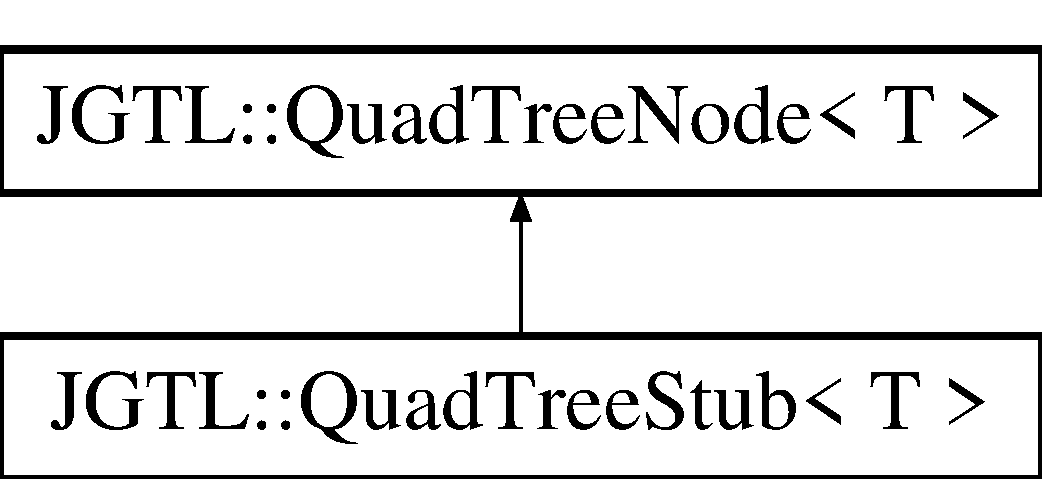
\includegraphics[height=2cm]{class_j_g_t_l_1_1_quad_tree_stub}
\end{center}
\end{figure}
\subsection*{Public Member Functions}
\begin{CompactItemize}
\item 
\hyperlink{class_j_g_t_l_1_1_quad_tree_stub_f93b1d865168c08ccfc5f9ceebaa8003}{Quad\-Tree\-Stub} (T \_\-value)
\item 
virtual \hyperlink{class_j_g_t_l_1_1_quad_tree_stub_6106651b6f6f285ad1bb469f823ef8ad}{$\sim$Quad\-Tree\-Stub} ()
\item 
virtual T \hyperlink{class_j_g_t_l_1_1_quad_tree_stub_99e89a45f21e503a1cef13f54a8ef65b}{get\-Value} (\hyperlink{class_j_g_t_l_1_1_vector2}{Vector2}$<$ int $>$ top\-Left\-Vector2, int size, const \hyperlink{class_j_g_t_l_1_1_vector2}{Vector2}$<$ int $>$ \&location) const 
\item 
virtual T \hyperlink{class_j_g_t_l_1_1_quad_tree_stub_48f2d4a15b1b8b850b9d446fe972f561}{get\-Value} () const
\item 
virtual bool \hyperlink{class_j_g_t_l_1_1_quad_tree_stub_a89e27cf98e753df813770d7007b7a9b}{set\-Value} (boost::pool$<$$>$ \&branch\-Pool, boost::pool$<$$>$ \&stub\-Pool, \hyperlink{class_j_g_t_l_1_1_vector2}{Vector2}$<$ int $>$ top\-Left\-Vector2, int size, const \hyperlink{class_j_g_t_l_1_1_vector2}{Vector2}$<$ int $>$ \&location, const T \&\hyperlink{class_j_g_t_l_1_1_quad_tree_stub_2b4f08acca095e6e2f3f92afc9f0449e}{value})
\item 
virtual bool \hyperlink{class_j_g_t_l_1_1_quad_tree_stub_8f3a3fc28ed6b8880b68ad791c1cb931}{set\-Value} (const T \&\_\-value)
\item 
virtual bool \hyperlink{class_j_g_t_l_1_1_quad_tree_stub_69d364f4525bbc32d27ad2a7a2a4502b}{is\-Stub} () const
\item 
virtual void \hyperlink{class_j_g_t_l_1_1_quad_tree_stub_d9cc4e6b8fb18dd55043edf3f503c9c7}{display} (int level) const
\end{CompactItemize}
\subsection*{Protected Attributes}
\begin{CompactItemize}
\item 
T \hyperlink{class_j_g_t_l_1_1_quad_tree_stub_2b4f08acca095e6e2f3f92afc9f0449e}{value}
\end{CompactItemize}
\subsubsection*{template$<$class T$>$ class JGTL::Quad\-Tree\-Stub$<$ T $>$}



\subsection{Constructor \& Destructor Documentation}
\hypertarget{class_j_g_t_l_1_1_quad_tree_stub_f93b1d865168c08ccfc5f9ceebaa8003}{
\index{JGTL::QuadTreeStub@{JGTL::Quad\-Tree\-Stub}!QuadTreeStub@{QuadTreeStub}}
\index{QuadTreeStub@{QuadTreeStub}!JGTL::QuadTreeStub@{JGTL::Quad\-Tree\-Stub}}
\subsubsection[QuadTreeStub]{\setlength{\rightskip}{0pt plus 5cm}template$<$class T$>$ \hyperlink{class_j_g_t_l_1_1_quad_tree_stub}{JGTL::Quad\-Tree\-Stub}$<$ T $>$::\hyperlink{class_j_g_t_l_1_1_quad_tree_stub}{Quad\-Tree\-Stub} (T {\em \_\-value})\hspace{0.3cm}{\tt  \mbox{[}inline\mbox{]}}}}
\label{class_j_g_t_l_1_1_quad_tree_stub_f93b1d865168c08ccfc5f9ceebaa8003}


\hypertarget{class_j_g_t_l_1_1_quad_tree_stub_6106651b6f6f285ad1bb469f823ef8ad}{
\index{JGTL::QuadTreeStub@{JGTL::Quad\-Tree\-Stub}!~QuadTreeStub@{$\sim$QuadTreeStub}}
\index{~QuadTreeStub@{$\sim$QuadTreeStub}!JGTL::QuadTreeStub@{JGTL::Quad\-Tree\-Stub}}
\subsubsection[$\sim$QuadTreeStub]{\setlength{\rightskip}{0pt plus 5cm}template$<$class T$>$ virtual \hyperlink{class_j_g_t_l_1_1_quad_tree_stub}{JGTL::Quad\-Tree\-Stub}$<$ T $>$::$\sim$\hyperlink{class_j_g_t_l_1_1_quad_tree_stub}{Quad\-Tree\-Stub} ()\hspace{0.3cm}{\tt  \mbox{[}inline, virtual\mbox{]}}}}
\label{class_j_g_t_l_1_1_quad_tree_stub_6106651b6f6f285ad1bb469f823ef8ad}




\subsection{Member Function Documentation}
\hypertarget{class_j_g_t_l_1_1_quad_tree_stub_99e89a45f21e503a1cef13f54a8ef65b}{
\index{JGTL::QuadTreeStub@{JGTL::Quad\-Tree\-Stub}!getValue@{getValue}}
\index{getValue@{getValue}!JGTL::QuadTreeStub@{JGTL::Quad\-Tree\-Stub}}
\subsubsection[getValue]{\setlength{\rightskip}{0pt plus 5cm}template$<$class T$>$ virtual T \hyperlink{class_j_g_t_l_1_1_quad_tree_stub}{JGTL::Quad\-Tree\-Stub}$<$ T $>$::get\-Value (\hyperlink{class_j_g_t_l_1_1_vector2}{Vector2}$<$ int $>$ {\em top\-Left\-Vector2}, int {\em size}, const \hyperlink{class_j_g_t_l_1_1_vector2}{Vector2}$<$ int $>$ \& {\em location}) const\hspace{0.3cm}{\tt  \mbox{[}inline, virtual\mbox{]}}}}
\label{class_j_g_t_l_1_1_quad_tree_stub_99e89a45f21e503a1cef13f54a8ef65b}




Implements \hyperlink{class_j_g_t_l_1_1_quad_tree_node_bc249b527b146888c21dac71783f42b6}{JGTL::Quad\-Tree\-Node$<$ T $>$}.\hypertarget{class_j_g_t_l_1_1_quad_tree_stub_48f2d4a15b1b8b850b9d446fe972f561}{
\index{JGTL::QuadTreeStub@{JGTL::Quad\-Tree\-Stub}!getValue@{getValue}}
\index{getValue@{getValue}!JGTL::QuadTreeStub@{JGTL::Quad\-Tree\-Stub}}
\subsubsection[getValue]{\setlength{\rightskip}{0pt plus 5cm}template$<$class T$>$ virtual T \hyperlink{class_j_g_t_l_1_1_quad_tree_stub}{JGTL::Quad\-Tree\-Stub}$<$ T $>$::get\-Value () const\hspace{0.3cm}{\tt  \mbox{[}inline, virtual\mbox{]}}}}
\label{class_j_g_t_l_1_1_quad_tree_stub_48f2d4a15b1b8b850b9d446fe972f561}




Implements \hyperlink{class_j_g_t_l_1_1_quad_tree_node_b92e9755284317f2d8102f028b0481c7}{JGTL::Quad\-Tree\-Node$<$ T $>$}.\hypertarget{class_j_g_t_l_1_1_quad_tree_stub_a89e27cf98e753df813770d7007b7a9b}{
\index{JGTL::QuadTreeStub@{JGTL::Quad\-Tree\-Stub}!setValue@{setValue}}
\index{setValue@{setValue}!JGTL::QuadTreeStub@{JGTL::Quad\-Tree\-Stub}}
\subsubsection[setValue]{\setlength{\rightskip}{0pt plus 5cm}template$<$class T$>$ virtual bool \hyperlink{class_j_g_t_l_1_1_quad_tree_stub}{JGTL::Quad\-Tree\-Stub}$<$ T $>$::set\-Value (boost::pool$<$$>$ \& {\em branch\-Pool}, boost::pool$<$$>$ \& {\em stub\-Pool}, \hyperlink{class_j_g_t_l_1_1_vector2}{Vector2}$<$ int $>$ {\em top\-Left\-Vector2}, int {\em size}, const \hyperlink{class_j_g_t_l_1_1_vector2}{Vector2}$<$ int $>$ \& {\em location}, const T \& {\em value})\hspace{0.3cm}{\tt  \mbox{[}inline, virtual\mbox{]}}}}
\label{class_j_g_t_l_1_1_quad_tree_stub_a89e27cf98e753df813770d7007b7a9b}




Implements \hyperlink{class_j_g_t_l_1_1_quad_tree_node_8bf383a824c1b5dc7dc2fff05aeaaec9}{JGTL::Quad\-Tree\-Node$<$ T $>$}.\hypertarget{class_j_g_t_l_1_1_quad_tree_stub_8f3a3fc28ed6b8880b68ad791c1cb931}{
\index{JGTL::QuadTreeStub@{JGTL::Quad\-Tree\-Stub}!setValue@{setValue}}
\index{setValue@{setValue}!JGTL::QuadTreeStub@{JGTL::Quad\-Tree\-Stub}}
\subsubsection[setValue]{\setlength{\rightskip}{0pt plus 5cm}template$<$class T$>$ virtual bool \hyperlink{class_j_g_t_l_1_1_quad_tree_stub}{JGTL::Quad\-Tree\-Stub}$<$ T $>$::set\-Value (const T \& {\em \_\-value})\hspace{0.3cm}{\tt  \mbox{[}inline, virtual\mbox{]}}}}
\label{class_j_g_t_l_1_1_quad_tree_stub_8f3a3fc28ed6b8880b68ad791c1cb931}


\hypertarget{class_j_g_t_l_1_1_quad_tree_stub_69d364f4525bbc32d27ad2a7a2a4502b}{
\index{JGTL::QuadTreeStub@{JGTL::Quad\-Tree\-Stub}!isStub@{isStub}}
\index{isStub@{isStub}!JGTL::QuadTreeStub@{JGTL::Quad\-Tree\-Stub}}
\subsubsection[isStub]{\setlength{\rightskip}{0pt plus 5cm}template$<$class T$>$ virtual bool \hyperlink{class_j_g_t_l_1_1_quad_tree_stub}{JGTL::Quad\-Tree\-Stub}$<$ T $>$::is\-Stub () const\hspace{0.3cm}{\tt  \mbox{[}inline, virtual\mbox{]}}}}
\label{class_j_g_t_l_1_1_quad_tree_stub_69d364f4525bbc32d27ad2a7a2a4502b}




Reimplemented from \hyperlink{class_j_g_t_l_1_1_quad_tree_node_bdc8677d8f2d61e8e7bbe31922b1899f}{JGTL::Quad\-Tree\-Node$<$ T $>$}.\hypertarget{class_j_g_t_l_1_1_quad_tree_stub_d9cc4e6b8fb18dd55043edf3f503c9c7}{
\index{JGTL::QuadTreeStub@{JGTL::Quad\-Tree\-Stub}!display@{display}}
\index{display@{display}!JGTL::QuadTreeStub@{JGTL::Quad\-Tree\-Stub}}
\subsubsection[display]{\setlength{\rightskip}{0pt plus 5cm}template$<$class T$>$ virtual void \hyperlink{class_j_g_t_l_1_1_quad_tree_stub}{JGTL::Quad\-Tree\-Stub}$<$ T $>$::display (int {\em level}) const\hspace{0.3cm}{\tt  \mbox{[}inline, virtual\mbox{]}}}}
\label{class_j_g_t_l_1_1_quad_tree_stub_d9cc4e6b8fb18dd55043edf3f503c9c7}




Implements \hyperlink{class_j_g_t_l_1_1_quad_tree_node_5d3e714f007be6a1ab507bcda173aede}{JGTL::Quad\-Tree\-Node$<$ T $>$}.

\subsection{Member Data Documentation}
\hypertarget{class_j_g_t_l_1_1_quad_tree_stub_2b4f08acca095e6e2f3f92afc9f0449e}{
\index{JGTL::QuadTreeStub@{JGTL::Quad\-Tree\-Stub}!value@{value}}
\index{value@{value}!JGTL::QuadTreeStub@{JGTL::Quad\-Tree\-Stub}}
\subsubsection[value]{\setlength{\rightskip}{0pt plus 5cm}template$<$class T$>$ T \hyperlink{class_j_g_t_l_1_1_quad_tree_stub}{JGTL::Quad\-Tree\-Stub}$<$ T $>$::\hyperlink{class_j_g_t_l_1_1_quad_tree_stub_2b4f08acca095e6e2f3f92afc9f0449e}{value}\hspace{0.3cm}{\tt  \mbox{[}protected\mbox{]}}}}
\label{class_j_g_t_l_1_1_quad_tree_stub_2b4f08acca095e6e2f3f92afc9f0449e}




The documentation for this class was generated from the following file:\begin{CompactItemize}
\item 
\hyperlink{_j_g_t_l___quad_tree_8h}{JGTL\_\-Quad\-Tree.h}\end{CompactItemize}

\hypertarget{class_j_g_t_l_1_1_ray2}{
\section{JGTL::Ray2$<$ T $>$ Class Template Reference}
\label{class_j_g_t_l_1_1_ray2}\index{JGTL::Ray2@{JGTL::Ray2}}
}
This class handles 2D Rays and Line Segments.  


{\tt \#include $<$JGTL\_\-Ray2.h$>$}

\subsection*{Public Member Functions}
\begin{CompactItemize}
\item 
\hyperlink{class_j_g_t_l_1_1_ray2_31284d7badc1d41327dbe9f968c66186}{Ray2} ()
\item 
template$<$class TT, class TTT$>$ \hyperlink{class_j_g_t_l_1_1_ray2_5ab2591d6df17a32373b34259913fbe2}{Ray2} (const \hyperlink{class_j_g_t_l_1_1_vector2}{Vector2}$<$ TT $>$ \&\_\-base, const \hyperlink{class_j_g_t_l_1_1_vector2}{Vector2}$<$ TTT $>$ \&\_\-direction)
\item 
\hyperlink{class_j_g_t_l_1_1_vector2}{Vector2}$<$ T $>$ \hyperlink{class_j_g_t_l_1_1_ray2_e3d5c3d3ba2693d7904dabfd6407cd32}{get\-Direction} () const
\item 
\hyperlink{class_j_g_t_l_1_1_vector2}{Vector2}$<$ T $>$ \hyperlink{class_j_g_t_l_1_1_ray2_151f4c434cde6776eb9183def4529944}{get\-Base} () const
\item 
\hyperlink{class_j_g_t_l_1_1_vector2}{Vector2}$<$ T $>$ \hyperlink{class_j_g_t_l_1_1_ray2_2b38de58f57dd042c582fe2f9aa9258a}{get\-End\-Point} () const
\item 
template$<$class TT$>$ void \hyperlink{class_j_g_t_l_1_1_ray2_188eb46e39c7240523863760a7afe756}{set\-Base} (const \hyperlink{class_j_g_t_l_1_1_vector2}{Vector2}$<$ TT $>$ \&new\-Base)
\item 
template$<$class TT$>$ void \hyperlink{class_j_g_t_l_1_1_ray2_cc31a907c03a3d013694d3f0ac476e47}{set\-Direction} (const \hyperlink{class_j_g_t_l_1_1_vector2}{Vector2}$<$ TT $>$ \&new\-Direction)
\item 
template$<$class TT$>$ T \hyperlink{class_j_g_t_l_1_1_ray2_32b3a18663a108c037713e0473180223}{get\-Projection\-TVal} (const \hyperlink{class_j_g_t_l_1_1_vector2}{Vector2}$<$ TT $>$ \&Vector) const 
\item 
\hyperlink{class_j_g_t_l_1_1_vector2}{Vector2}$<$ T $>$ \hyperlink{class_j_g_t_l_1_1_ray2_e59574fde082ff15adf09d6597782447}{get\-Projection\-Vector} (T t) const 
\item 
void \hyperlink{class_j_g_t_l_1_1_ray2_ac8af5ab11d2371da705144c47f2913b}{normalize} ()
\item 
template$<$class TT$>$ std::pair$<$ \hyperlink{namespace_j_g_t_l_84ea7d7d885581de216d16c16850615a}{Intersection\-State}, float $>$ \hyperlink{class_j_g_t_l_1_1_ray2_f520be1d874ef1679798e3c2b24a23ed}{get\-Intersection} (const \hyperlink{class_j_g_t_l_1_1_ray2}{Ray2}$<$ TT $>$ \&other, bool line\-Segment=false) const 
\end{CompactItemize}
\subsection*{Protected Member Functions}
\begin{CompactItemize}
\item 
bool \hyperlink{class_j_g_t_l_1_1_ray2_c41c241bb8ef64b63d43a9c5aaef78d9}{within} (T a, T b, T c) const
\item 
bool \hyperlink{class_j_g_t_l_1_1_ray2_206fd5a155f3d460b878ea94f8df3eb2}{putwhere} (T x, T y, \hyperlink{class_j_g_t_l_1_1_vector2}{Vector2}$<$ T $>$ \&where, bool first) const 
\end{CompactItemize}
\subsection*{Protected Attributes}
\begin{CompactItemize}
\item 
\hyperlink{class_j_g_t_l_1_1_vector2}{Vector2}$<$ T $>$ \hyperlink{class_j_g_t_l_1_1_ray2_5a70c3e1b6e6e940feaf0a45ab377f34}{base}
\item 
\hyperlink{class_j_g_t_l_1_1_vector2}{Vector2}$<$ T $>$ \hyperlink{class_j_g_t_l_1_1_ray2_cb20b77d19a22288144189f326a4fa79}{direction}
\end{CompactItemize}


\subsection{Detailed Description}
\subsubsection*{template$<$class T$>$ class JGTL::Ray2$<$ T $>$}

This class handles 2D Rays and Line Segments. 

\begin{Desc}
\item[Author:]Jason Gauci \end{Desc}
\begin{Desc}
\item[Date:]2008 \end{Desc}




\subsection{Constructor \& Destructor Documentation}
\hypertarget{class_j_g_t_l_1_1_ray2_31284d7badc1d41327dbe9f968c66186}{
\index{JGTL::Ray2@{JGTL::Ray2}!Ray2@{Ray2}}
\index{Ray2@{Ray2}!JGTL::Ray2@{JGTL::Ray2}}
\subsubsection[Ray2]{\setlength{\rightskip}{0pt plus 5cm}template$<$class T$>$ \hyperlink{class_j_g_t_l_1_1_ray2}{JGTL::Ray2}$<$ T $>$::\hyperlink{class_j_g_t_l_1_1_ray2}{Ray2} ()\hspace{0.3cm}{\tt  \mbox{[}inline\mbox{]}}}}
\label{class_j_g_t_l_1_1_ray2_31284d7badc1d41327dbe9f968c66186}


\hypertarget{class_j_g_t_l_1_1_ray2_5ab2591d6df17a32373b34259913fbe2}{
\index{JGTL::Ray2@{JGTL::Ray2}!Ray2@{Ray2}}
\index{Ray2@{Ray2}!JGTL::Ray2@{JGTL::Ray2}}
\subsubsection[Ray2]{\setlength{\rightskip}{0pt plus 5cm}template$<$class T$>$ template$<$class TT, class TTT$>$ \hyperlink{class_j_g_t_l_1_1_ray2}{JGTL::Ray2}$<$ T $>$::\hyperlink{class_j_g_t_l_1_1_ray2}{Ray2} (const \hyperlink{class_j_g_t_l_1_1_vector2}{Vector2}$<$ TT $>$ \& {\em \_\-base}, const \hyperlink{class_j_g_t_l_1_1_vector2}{Vector2}$<$ TTT $>$ \& {\em \_\-direction})\hspace{0.3cm}{\tt  \mbox{[}inline\mbox{]}}}}
\label{class_j_g_t_l_1_1_ray2_5ab2591d6df17a32373b34259913fbe2}




\subsection{Member Function Documentation}
\hypertarget{class_j_g_t_l_1_1_ray2_e3d5c3d3ba2693d7904dabfd6407cd32}{
\index{JGTL::Ray2@{JGTL::Ray2}!getDirection@{getDirection}}
\index{getDirection@{getDirection}!JGTL::Ray2@{JGTL::Ray2}}
\subsubsection[getDirection]{\setlength{\rightskip}{0pt plus 5cm}template$<$class T$>$ \hyperlink{class_j_g_t_l_1_1_vector2}{Vector2}$<$T$>$ \hyperlink{class_j_g_t_l_1_1_ray2}{JGTL::Ray2}$<$ T $>$::get\-Direction () const\hspace{0.3cm}{\tt  \mbox{[}inline\mbox{]}}}}
\label{class_j_g_t_l_1_1_ray2_e3d5c3d3ba2693d7904dabfd6407cd32}


\hypertarget{class_j_g_t_l_1_1_ray2_151f4c434cde6776eb9183def4529944}{
\index{JGTL::Ray2@{JGTL::Ray2}!getBase@{getBase}}
\index{getBase@{getBase}!JGTL::Ray2@{JGTL::Ray2}}
\subsubsection[getBase]{\setlength{\rightskip}{0pt plus 5cm}template$<$class T$>$ \hyperlink{class_j_g_t_l_1_1_vector2}{Vector2}$<$T$>$ \hyperlink{class_j_g_t_l_1_1_ray2}{JGTL::Ray2}$<$ T $>$::get\-Base () const\hspace{0.3cm}{\tt  \mbox{[}inline\mbox{]}}}}
\label{class_j_g_t_l_1_1_ray2_151f4c434cde6776eb9183def4529944}


\hypertarget{class_j_g_t_l_1_1_ray2_2b38de58f57dd042c582fe2f9aa9258a}{
\index{JGTL::Ray2@{JGTL::Ray2}!getEndPoint@{getEndPoint}}
\index{getEndPoint@{getEndPoint}!JGTL::Ray2@{JGTL::Ray2}}
\subsubsection[getEndPoint]{\setlength{\rightskip}{0pt plus 5cm}template$<$class T$>$ \hyperlink{class_j_g_t_l_1_1_vector2}{Vector2}$<$T$>$ \hyperlink{class_j_g_t_l_1_1_ray2}{JGTL::Ray2}$<$ T $>$::get\-End\-Point () const\hspace{0.3cm}{\tt  \mbox{[}inline\mbox{]}}}}
\label{class_j_g_t_l_1_1_ray2_2b38de58f57dd042c582fe2f9aa9258a}


\hypertarget{class_j_g_t_l_1_1_ray2_188eb46e39c7240523863760a7afe756}{
\index{JGTL::Ray2@{JGTL::Ray2}!setBase@{setBase}}
\index{setBase@{setBase}!JGTL::Ray2@{JGTL::Ray2}}
\subsubsection[setBase]{\setlength{\rightskip}{0pt plus 5cm}template$<$class T$>$ template$<$class TT$>$ void \hyperlink{class_j_g_t_l_1_1_ray2}{JGTL::Ray2}$<$ T $>$::set\-Base (const \hyperlink{class_j_g_t_l_1_1_vector2}{Vector2}$<$ TT $>$ \& {\em new\-Base})\hspace{0.3cm}{\tt  \mbox{[}inline\mbox{]}}}}
\label{class_j_g_t_l_1_1_ray2_188eb46e39c7240523863760a7afe756}


\hypertarget{class_j_g_t_l_1_1_ray2_cc31a907c03a3d013694d3f0ac476e47}{
\index{JGTL::Ray2@{JGTL::Ray2}!setDirection@{setDirection}}
\index{setDirection@{setDirection}!JGTL::Ray2@{JGTL::Ray2}}
\subsubsection[setDirection]{\setlength{\rightskip}{0pt plus 5cm}template$<$class T$>$ template$<$class TT$>$ void \hyperlink{class_j_g_t_l_1_1_ray2}{JGTL::Ray2}$<$ T $>$::set\-Direction (const \hyperlink{class_j_g_t_l_1_1_vector2}{Vector2}$<$ TT $>$ \& {\em new\-Direction})\hspace{0.3cm}{\tt  \mbox{[}inline\mbox{]}}}}
\label{class_j_g_t_l_1_1_ray2_cc31a907c03a3d013694d3f0ac476e47}


\hypertarget{class_j_g_t_l_1_1_ray2_32b3a18663a108c037713e0473180223}{
\index{JGTL::Ray2@{JGTL::Ray2}!getProjectionTVal@{getProjectionTVal}}
\index{getProjectionTVal@{getProjectionTVal}!JGTL::Ray2@{JGTL::Ray2}}
\subsubsection[getProjectionTVal]{\setlength{\rightskip}{0pt plus 5cm}template$<$class T$>$ template$<$class TT$>$ T \hyperlink{class_j_g_t_l_1_1_ray2}{JGTL::Ray2}$<$ T $>$::get\-Projection\-TVal (const \hyperlink{class_j_g_t_l_1_1_vector2}{Vector2}$<$ TT $>$ \& {\em Vector}) const\hspace{0.3cm}{\tt  \mbox{[}inline\mbox{]}}}}
\label{class_j_g_t_l_1_1_ray2_32b3a18663a108c037713e0473180223}


\hypertarget{class_j_g_t_l_1_1_ray2_e59574fde082ff15adf09d6597782447}{
\index{JGTL::Ray2@{JGTL::Ray2}!getProjectionVector@{getProjectionVector}}
\index{getProjectionVector@{getProjectionVector}!JGTL::Ray2@{JGTL::Ray2}}
\subsubsection[getProjectionVector]{\setlength{\rightskip}{0pt plus 5cm}template$<$class T$>$ \hyperlink{class_j_g_t_l_1_1_vector2}{Vector2}$<$T$>$ \hyperlink{class_j_g_t_l_1_1_ray2}{JGTL::Ray2}$<$ T $>$::get\-Projection\-Vector (T {\em t}) const\hspace{0.3cm}{\tt  \mbox{[}inline\mbox{]}}}}
\label{class_j_g_t_l_1_1_ray2_e59574fde082ff15adf09d6597782447}


\hypertarget{class_j_g_t_l_1_1_ray2_ac8af5ab11d2371da705144c47f2913b}{
\index{JGTL::Ray2@{JGTL::Ray2}!normalize@{normalize}}
\index{normalize@{normalize}!JGTL::Ray2@{JGTL::Ray2}}
\subsubsection[normalize]{\setlength{\rightskip}{0pt plus 5cm}template$<$class T$>$ void \hyperlink{class_j_g_t_l_1_1_ray2}{JGTL::Ray2}$<$ T $>$::normalize ()\hspace{0.3cm}{\tt  \mbox{[}inline\mbox{]}}}}
\label{class_j_g_t_l_1_1_ray2_ac8af5ab11d2371da705144c47f2913b}


\hypertarget{class_j_g_t_l_1_1_ray2_f520be1d874ef1679798e3c2b24a23ed}{
\index{JGTL::Ray2@{JGTL::Ray2}!getIntersection@{getIntersection}}
\index{getIntersection@{getIntersection}!JGTL::Ray2@{JGTL::Ray2}}
\subsubsection[getIntersection]{\setlength{\rightskip}{0pt plus 5cm}template$<$class T$>$ template$<$class TT$>$ std::pair$<$\hyperlink{namespace_j_g_t_l_84ea7d7d885581de216d16c16850615a}{Intersection\-State},float$>$ \hyperlink{class_j_g_t_l_1_1_ray2}{JGTL::Ray2}$<$ T $>$::get\-Intersection (const \hyperlink{class_j_g_t_l_1_1_ray2}{Ray2}$<$ TT $>$ \& {\em other}, bool {\em line\-Segment} = {\tt false}) const\hspace{0.3cm}{\tt  \mbox{[}inline\mbox{]}}}}
\label{class_j_g_t_l_1_1_ray2_f520be1d874ef1679798e3c2b24a23ed}


\hypertarget{class_j_g_t_l_1_1_ray2_c41c241bb8ef64b63d43a9c5aaef78d9}{
\index{JGTL::Ray2@{JGTL::Ray2}!within@{within}}
\index{within@{within}!JGTL::Ray2@{JGTL::Ray2}}
\subsubsection[within]{\setlength{\rightskip}{0pt plus 5cm}template$<$class T$>$ bool \hyperlink{class_j_g_t_l_1_1_ray2}{JGTL::Ray2}$<$ T $>$::within (T {\em a}, T {\em b}, T {\em c}) const\hspace{0.3cm}{\tt  \mbox{[}inline, protected\mbox{]}}}}
\label{class_j_g_t_l_1_1_ray2_c41c241bb8ef64b63d43a9c5aaef78d9}


\hypertarget{class_j_g_t_l_1_1_ray2_206fd5a155f3d460b878ea94f8df3eb2}{
\index{JGTL::Ray2@{JGTL::Ray2}!putwhere@{putwhere}}
\index{putwhere@{putwhere}!JGTL::Ray2@{JGTL::Ray2}}
\subsubsection[putwhere]{\setlength{\rightskip}{0pt plus 5cm}template$<$class T$>$ bool \hyperlink{class_j_g_t_l_1_1_ray2}{JGTL::Ray2}$<$ T $>$::putwhere (T {\em x}, T {\em y}, \hyperlink{class_j_g_t_l_1_1_vector2}{Vector2}$<$ T $>$ \& {\em where}, bool {\em first}) const\hspace{0.3cm}{\tt  \mbox{[}inline, protected\mbox{]}}}}
\label{class_j_g_t_l_1_1_ray2_206fd5a155f3d460b878ea94f8df3eb2}




\subsection{Member Data Documentation}
\hypertarget{class_j_g_t_l_1_1_ray2_5a70c3e1b6e6e940feaf0a45ab377f34}{
\index{JGTL::Ray2@{JGTL::Ray2}!base@{base}}
\index{base@{base}!JGTL::Ray2@{JGTL::Ray2}}
\subsubsection[base]{\setlength{\rightskip}{0pt plus 5cm}template$<$class T$>$ \hyperlink{class_j_g_t_l_1_1_vector2}{Vector2}$<$T$>$ \hyperlink{class_j_g_t_l_1_1_ray2}{JGTL::Ray2}$<$ T $>$::\hyperlink{class_j_g_t_l_1_1_ray2_5a70c3e1b6e6e940feaf0a45ab377f34}{base}\hspace{0.3cm}{\tt  \mbox{[}protected\mbox{]}}}}
\label{class_j_g_t_l_1_1_ray2_5a70c3e1b6e6e940feaf0a45ab377f34}


\hypertarget{class_j_g_t_l_1_1_ray2_cb20b77d19a22288144189f326a4fa79}{
\index{JGTL::Ray2@{JGTL::Ray2}!direction@{direction}}
\index{direction@{direction}!JGTL::Ray2@{JGTL::Ray2}}
\subsubsection[direction]{\setlength{\rightskip}{0pt plus 5cm}template$<$class T$>$ \hyperlink{class_j_g_t_l_1_1_vector2}{Vector2}$<$T$>$ \hyperlink{class_j_g_t_l_1_1_ray2}{JGTL::Ray2}$<$ T $>$::\hyperlink{class_j_g_t_l_1_1_ray2_cb20b77d19a22288144189f326a4fa79}{direction}\hspace{0.3cm}{\tt  \mbox{[}protected\mbox{]}}}}
\label{class_j_g_t_l_1_1_ray2_cb20b77d19a22288144189f326a4fa79}




The documentation for this class was generated from the following file:\begin{CompactItemize}
\item 
\hyperlink{_j_g_t_l___ray2_8h}{JGTL\_\-Ray2.h}\end{CompactItemize}

\hypertarget{class_j_g_t_l_1_1_ray3}{
\section{JGTL::Ray3$<$ T $>$ Class Template Reference}
\label{class_j_g_t_l_1_1_ray3}\index{JGTL::Ray3@{JGTL::Ray3}}
}
This class handles 3D Rays and Line Segments.  


{\tt \#include $<$JGTL\_\-Ray3.h$>$}

\subsection*{Public Member Functions}
\begin{CompactItemize}
\item 
\hyperlink{class_j_g_t_l_1_1_ray3_4bb85483d586f50f9b322bf93e861da5}{Ray3} ()
\item 
template$<$class TT, class TTT$>$ \hyperlink{class_j_g_t_l_1_1_ray3_1a31f0cc4568493c7de6c9c6571f63c5}{Ray3} (const \hyperlink{class_j_g_t_l_1_1_vector3}{Vector3}$<$ TT $>$ \&\_\-base, const \hyperlink{class_j_g_t_l_1_1_vector3}{Vector3}$<$ TTT $>$ \&\_\-direction)
\item 
\hyperlink{class_j_g_t_l_1_1_vector3}{Vector3}$<$ T $>$ \hyperlink{class_j_g_t_l_1_1_ray3_67bf186dce63bb65f0b5ad105e0d2418}{get\-Direction} () const
\item 
\hyperlink{class_j_g_t_l_1_1_vector3}{Vector3}$<$ T $>$ \hyperlink{class_j_g_t_l_1_1_ray3_2889303af0d3c3aaf7b24b4fb841613c}{get\-Base} () const
\item 
template$<$class TT$>$ void \hyperlink{class_j_g_t_l_1_1_ray3_61e6030f02fd3ba346634c808054962f}{set\-Base} (\hyperlink{class_j_g_t_l_1_1_vector3}{Vector3}$<$ TT $>$ new\-Base)
\item 
template$<$class TT$>$ void \hyperlink{class_j_g_t_l_1_1_ray3_eaa2bcbd6fa914eab2c653e2053ce42b}{set\-Direction} (const \hyperlink{class_j_g_t_l_1_1_vector3}{Vector3}$<$ TT $>$ \&new\-Direction)
\item 
template$<$class TT$>$ T \hyperlink{class_j_g_t_l_1_1_ray3_a82c4c7c60beee84f42dae8329bafebd}{get\-Projection\-TVal} (const \hyperlink{class_j_g_t_l_1_1_vector3}{Vector3}$<$ TT $>$ \&Vector) const 
\item 
\hyperlink{class_j_g_t_l_1_1_vector3}{Vector3}$<$ T $>$ \hyperlink{class_j_g_t_l_1_1_ray3_39b7bca999aefc20548add34db248989}{get\-Projection\-Vector} (T t) const 
\item 
void \hyperlink{class_j_g_t_l_1_1_ray3_939795292a630247cd6d0eb27bd17527}{normalize} ()
\end{CompactItemize}
\subsection*{Protected Attributes}
\begin{CompactItemize}
\item 
\hyperlink{class_j_g_t_l_1_1_vector3}{Vector3}$<$ T $>$ \hyperlink{class_j_g_t_l_1_1_ray3_7f6edc8423bebe5ad9147f216766c4cf}{base}
\item 
\hyperlink{class_j_g_t_l_1_1_vector3}{Vector3}$<$ T $>$ \hyperlink{class_j_g_t_l_1_1_ray3_611f05fc7fab5c587ae5d13aeed02b03}{direction}
\end{CompactItemize}


\subsection{Detailed Description}
\subsubsection*{template$<$class T$>$ class JGTL::Ray3$<$ T $>$}

This class handles 3D Rays and Line Segments. 

\begin{Desc}
\item[Author:]Jason Gauci \end{Desc}
\begin{Desc}
\item[Date:]2008 \end{Desc}




\subsection{Constructor \& Destructor Documentation}
\hypertarget{class_j_g_t_l_1_1_ray3_4bb85483d586f50f9b322bf93e861da5}{
\index{JGTL::Ray3@{JGTL::Ray3}!Ray3@{Ray3}}
\index{Ray3@{Ray3}!JGTL::Ray3@{JGTL::Ray3}}
\subsubsection[Ray3]{\setlength{\rightskip}{0pt plus 5cm}template$<$class T$>$ \hyperlink{class_j_g_t_l_1_1_ray3}{JGTL::Ray3}$<$ T $>$::\hyperlink{class_j_g_t_l_1_1_ray3}{Ray3} ()\hspace{0.3cm}{\tt  \mbox{[}inline\mbox{]}}}}
\label{class_j_g_t_l_1_1_ray3_4bb85483d586f50f9b322bf93e861da5}


\hypertarget{class_j_g_t_l_1_1_ray3_1a31f0cc4568493c7de6c9c6571f63c5}{
\index{JGTL::Ray3@{JGTL::Ray3}!Ray3@{Ray3}}
\index{Ray3@{Ray3}!JGTL::Ray3@{JGTL::Ray3}}
\subsubsection[Ray3]{\setlength{\rightskip}{0pt plus 5cm}template$<$class T$>$ template$<$class TT, class TTT$>$ \hyperlink{class_j_g_t_l_1_1_ray3}{JGTL::Ray3}$<$ T $>$::\hyperlink{class_j_g_t_l_1_1_ray3}{Ray3} (const \hyperlink{class_j_g_t_l_1_1_vector3}{Vector3}$<$ TT $>$ \& {\em \_\-base}, const \hyperlink{class_j_g_t_l_1_1_vector3}{Vector3}$<$ TTT $>$ \& {\em \_\-direction})\hspace{0.3cm}{\tt  \mbox{[}inline\mbox{]}}}}
\label{class_j_g_t_l_1_1_ray3_1a31f0cc4568493c7de6c9c6571f63c5}




\subsection{Member Function Documentation}
\hypertarget{class_j_g_t_l_1_1_ray3_67bf186dce63bb65f0b5ad105e0d2418}{
\index{JGTL::Ray3@{JGTL::Ray3}!getDirection@{getDirection}}
\index{getDirection@{getDirection}!JGTL::Ray3@{JGTL::Ray3}}
\subsubsection[getDirection]{\setlength{\rightskip}{0pt plus 5cm}template$<$class T$>$ \hyperlink{class_j_g_t_l_1_1_vector3}{Vector3}$<$T$>$ \hyperlink{class_j_g_t_l_1_1_ray3}{JGTL::Ray3}$<$ T $>$::get\-Direction () const\hspace{0.3cm}{\tt  \mbox{[}inline\mbox{]}}}}
\label{class_j_g_t_l_1_1_ray3_67bf186dce63bb65f0b5ad105e0d2418}


\hypertarget{class_j_g_t_l_1_1_ray3_2889303af0d3c3aaf7b24b4fb841613c}{
\index{JGTL::Ray3@{JGTL::Ray3}!getBase@{getBase}}
\index{getBase@{getBase}!JGTL::Ray3@{JGTL::Ray3}}
\subsubsection[getBase]{\setlength{\rightskip}{0pt plus 5cm}template$<$class T$>$ \hyperlink{class_j_g_t_l_1_1_vector3}{Vector3}$<$T$>$ \hyperlink{class_j_g_t_l_1_1_ray3}{JGTL::Ray3}$<$ T $>$::get\-Base () const\hspace{0.3cm}{\tt  \mbox{[}inline\mbox{]}}}}
\label{class_j_g_t_l_1_1_ray3_2889303af0d3c3aaf7b24b4fb841613c}


\hypertarget{class_j_g_t_l_1_1_ray3_61e6030f02fd3ba346634c808054962f}{
\index{JGTL::Ray3@{JGTL::Ray3}!setBase@{setBase}}
\index{setBase@{setBase}!JGTL::Ray3@{JGTL::Ray3}}
\subsubsection[setBase]{\setlength{\rightskip}{0pt plus 5cm}template$<$class T$>$ template$<$class TT$>$ void \hyperlink{class_j_g_t_l_1_1_ray3}{JGTL::Ray3}$<$ T $>$::set\-Base (\hyperlink{class_j_g_t_l_1_1_vector3}{Vector3}$<$ TT $>$ {\em new\-Base})\hspace{0.3cm}{\tt  \mbox{[}inline\mbox{]}}}}
\label{class_j_g_t_l_1_1_ray3_61e6030f02fd3ba346634c808054962f}


\hypertarget{class_j_g_t_l_1_1_ray3_eaa2bcbd6fa914eab2c653e2053ce42b}{
\index{JGTL::Ray3@{JGTL::Ray3}!setDirection@{setDirection}}
\index{setDirection@{setDirection}!JGTL::Ray3@{JGTL::Ray3}}
\subsubsection[setDirection]{\setlength{\rightskip}{0pt plus 5cm}template$<$class T$>$ template$<$class TT$>$ void \hyperlink{class_j_g_t_l_1_1_ray3}{JGTL::Ray3}$<$ T $>$::set\-Direction (const \hyperlink{class_j_g_t_l_1_1_vector3}{Vector3}$<$ TT $>$ \& {\em new\-Direction})\hspace{0.3cm}{\tt  \mbox{[}inline\mbox{]}}}}
\label{class_j_g_t_l_1_1_ray3_eaa2bcbd6fa914eab2c653e2053ce42b}


\hypertarget{class_j_g_t_l_1_1_ray3_a82c4c7c60beee84f42dae8329bafebd}{
\index{JGTL::Ray3@{JGTL::Ray3}!getProjectionTVal@{getProjectionTVal}}
\index{getProjectionTVal@{getProjectionTVal}!JGTL::Ray3@{JGTL::Ray3}}
\subsubsection[getProjectionTVal]{\setlength{\rightskip}{0pt plus 5cm}template$<$class T$>$ template$<$class TT$>$ T \hyperlink{class_j_g_t_l_1_1_ray3}{JGTL::Ray3}$<$ T $>$::get\-Projection\-TVal (const \hyperlink{class_j_g_t_l_1_1_vector3}{Vector3}$<$ TT $>$ \& {\em Vector}) const\hspace{0.3cm}{\tt  \mbox{[}inline\mbox{]}}}}
\label{class_j_g_t_l_1_1_ray3_a82c4c7c60beee84f42dae8329bafebd}


\hypertarget{class_j_g_t_l_1_1_ray3_39b7bca999aefc20548add34db248989}{
\index{JGTL::Ray3@{JGTL::Ray3}!getProjectionVector@{getProjectionVector}}
\index{getProjectionVector@{getProjectionVector}!JGTL::Ray3@{JGTL::Ray3}}
\subsubsection[getProjectionVector]{\setlength{\rightskip}{0pt plus 5cm}template$<$class T$>$ \hyperlink{class_j_g_t_l_1_1_vector3}{Vector3}$<$T$>$ \hyperlink{class_j_g_t_l_1_1_ray3}{JGTL::Ray3}$<$ T $>$::get\-Projection\-Vector (T {\em t}) const\hspace{0.3cm}{\tt  \mbox{[}inline\mbox{]}}}}
\label{class_j_g_t_l_1_1_ray3_39b7bca999aefc20548add34db248989}


\hypertarget{class_j_g_t_l_1_1_ray3_939795292a630247cd6d0eb27bd17527}{
\index{JGTL::Ray3@{JGTL::Ray3}!normalize@{normalize}}
\index{normalize@{normalize}!JGTL::Ray3@{JGTL::Ray3}}
\subsubsection[normalize]{\setlength{\rightskip}{0pt plus 5cm}template$<$class T$>$ void \hyperlink{class_j_g_t_l_1_1_ray3}{JGTL::Ray3}$<$ T $>$::normalize ()\hspace{0.3cm}{\tt  \mbox{[}inline\mbox{]}}}}
\label{class_j_g_t_l_1_1_ray3_939795292a630247cd6d0eb27bd17527}




\subsection{Member Data Documentation}
\hypertarget{class_j_g_t_l_1_1_ray3_7f6edc8423bebe5ad9147f216766c4cf}{
\index{JGTL::Ray3@{JGTL::Ray3}!base@{base}}
\index{base@{base}!JGTL::Ray3@{JGTL::Ray3}}
\subsubsection[base]{\setlength{\rightskip}{0pt plus 5cm}template$<$class T$>$ \hyperlink{class_j_g_t_l_1_1_vector3}{Vector3}$<$T$>$ \hyperlink{class_j_g_t_l_1_1_ray3}{JGTL::Ray3}$<$ T $>$::\hyperlink{class_j_g_t_l_1_1_ray3_7f6edc8423bebe5ad9147f216766c4cf}{base}\hspace{0.3cm}{\tt  \mbox{[}protected\mbox{]}}}}
\label{class_j_g_t_l_1_1_ray3_7f6edc8423bebe5ad9147f216766c4cf}


\hypertarget{class_j_g_t_l_1_1_ray3_611f05fc7fab5c587ae5d13aeed02b03}{
\index{JGTL::Ray3@{JGTL::Ray3}!direction@{direction}}
\index{direction@{direction}!JGTL::Ray3@{JGTL::Ray3}}
\subsubsection[direction]{\setlength{\rightskip}{0pt plus 5cm}template$<$class T$>$ \hyperlink{class_j_g_t_l_1_1_vector3}{Vector3}$<$T$>$ \hyperlink{class_j_g_t_l_1_1_ray3}{JGTL::Ray3}$<$ T $>$::\hyperlink{class_j_g_t_l_1_1_ray3_611f05fc7fab5c587ae5d13aeed02b03}{direction}\hspace{0.3cm}{\tt  \mbox{[}protected\mbox{]}}}}
\label{class_j_g_t_l_1_1_ray3_611f05fc7fab5c587ae5d13aeed02b03}




The documentation for this class was generated from the following file:\begin{CompactItemize}
\item 
\hyperlink{_j_g_t_l___ray3_8h}{JGTL\_\-Ray3.h}\end{CompactItemize}

\hypertarget{class_j_g_t_l_1_1_rectangle3}{
\section{JGTL::Rectangle3$<$ T $>$ Class Template Reference}
\label{class_j_g_t_l_1_1_rectangle3}\index{JGTL::Rectangle3@{JGTL::Rectangle3}}
}
{\tt \#include $<$JGTL\_\-Rectangle3.h$>$}

\subsection*{Public Member Functions}
\begin{CompactItemize}
\item 
\hyperlink{class_j_g_t_l_1_1_rectangle3_95d1120ba01aa98bfd5a459b0c9a6a12}{Rectangle3} ()
\item 
\hyperlink{class_j_g_t_l_1_1_rectangle3_7907c71bb953badbd9f68501e0bb9b8a}{Rectangle3} (const \hyperlink{class_j_g_t_l_1_1_vector3}{Vector3}$<$ T $>$ \&\_\-top\-Left, const \hyperlink{class_j_g_t_l_1_1_vector3}{Vector3}$<$ T $>$ \&\_\-size)
\item 
bool \hyperlink{class_j_g_t_l_1_1_rectangle3_51f62ab3daf886c38057a72ecd0010d8}{contains} (const \hyperlink{class_j_g_t_l_1_1_vector3}{Vector3}$<$ T $>$ \&point) const 
\item 
const \hyperlink{class_j_g_t_l_1_1_vector3}{Vector3}$<$ T $>$ \& \hyperlink{class_j_g_t_l_1_1_rectangle3_66013d1d9cd1a51a4e1a9a2708098a6e}{get\-First\-Point} () const
\item 
bool \hyperlink{class_j_g_t_l_1_1_rectangle3_83b4f2996e51b68f6a14b0c1f1c35595}{get\-Next\-Discrete\-Point} (\hyperlink{class_j_g_t_l_1_1_vector3}{Vector3}$<$ T $>$ \&current\-Point) const 
\end{CompactItemize}
\subsection*{Public Attributes}
\begin{CompactItemize}
\item 
\hyperlink{class_j_g_t_l_1_1_vector3}{Vector3}$<$ T $>$ \hyperlink{class_j_g_t_l_1_1_rectangle3_9970035e43da1a163aa13b8bba5c1193}{top\-Left}
\item 
\hyperlink{class_j_g_t_l_1_1_vector3}{Vector3}$<$ T $>$ \hyperlink{class_j_g_t_l_1_1_rectangle3_9f63a1e076b374db4ebfa32de77ed4a5}{size}
\end{CompactItemize}
\subsubsection*{template$<$class T$>$ class JGTL::Rectangle3$<$ T $>$}



\subsection{Constructor \& Destructor Documentation}
\hypertarget{class_j_g_t_l_1_1_rectangle3_95d1120ba01aa98bfd5a459b0c9a6a12}{
\index{JGTL::Rectangle3@{JGTL::Rectangle3}!Rectangle3@{Rectangle3}}
\index{Rectangle3@{Rectangle3}!JGTL::Rectangle3@{JGTL::Rectangle3}}
\subsubsection[Rectangle3]{\setlength{\rightskip}{0pt plus 5cm}template$<$class T$>$ \hyperlink{class_j_g_t_l_1_1_rectangle3}{JGTL::Rectangle3}$<$ T $>$::\hyperlink{class_j_g_t_l_1_1_rectangle3}{Rectangle3} ()\hspace{0.3cm}{\tt  \mbox{[}inline\mbox{]}}}}
\label{class_j_g_t_l_1_1_rectangle3_95d1120ba01aa98bfd5a459b0c9a6a12}


\hypertarget{class_j_g_t_l_1_1_rectangle3_7907c71bb953badbd9f68501e0bb9b8a}{
\index{JGTL::Rectangle3@{JGTL::Rectangle3}!Rectangle3@{Rectangle3}}
\index{Rectangle3@{Rectangle3}!JGTL::Rectangle3@{JGTL::Rectangle3}}
\subsubsection[Rectangle3]{\setlength{\rightskip}{0pt plus 5cm}template$<$class T$>$ \hyperlink{class_j_g_t_l_1_1_rectangle3}{JGTL::Rectangle3}$<$ T $>$::\hyperlink{class_j_g_t_l_1_1_rectangle3}{Rectangle3} (const \hyperlink{class_j_g_t_l_1_1_vector3}{Vector3}$<$ T $>$ \& {\em \_\-top\-Left}, const \hyperlink{class_j_g_t_l_1_1_vector3}{Vector3}$<$ T $>$ \& {\em \_\-size})\hspace{0.3cm}{\tt  \mbox{[}inline\mbox{]}}}}
\label{class_j_g_t_l_1_1_rectangle3_7907c71bb953badbd9f68501e0bb9b8a}




\subsection{Member Function Documentation}
\hypertarget{class_j_g_t_l_1_1_rectangle3_51f62ab3daf886c38057a72ecd0010d8}{
\index{JGTL::Rectangle3@{JGTL::Rectangle3}!contains@{contains}}
\index{contains@{contains}!JGTL::Rectangle3@{JGTL::Rectangle3}}
\subsubsection[contains]{\setlength{\rightskip}{0pt plus 5cm}template$<$class T$>$ bool \hyperlink{class_j_g_t_l_1_1_rectangle3}{JGTL::Rectangle3}$<$ T $>$::contains (const \hyperlink{class_j_g_t_l_1_1_vector3}{Vector3}$<$ T $>$ \& {\em point}) const\hspace{0.3cm}{\tt  \mbox{[}inline\mbox{]}}}}
\label{class_j_g_t_l_1_1_rectangle3_51f62ab3daf886c38057a72ecd0010d8}


\hypertarget{class_j_g_t_l_1_1_rectangle3_66013d1d9cd1a51a4e1a9a2708098a6e}{
\index{JGTL::Rectangle3@{JGTL::Rectangle3}!getFirstPoint@{getFirstPoint}}
\index{getFirstPoint@{getFirstPoint}!JGTL::Rectangle3@{JGTL::Rectangle3}}
\subsubsection[getFirstPoint]{\setlength{\rightskip}{0pt plus 5cm}template$<$class T$>$ const \hyperlink{class_j_g_t_l_1_1_vector3}{Vector3}$<$T$>$\& \hyperlink{class_j_g_t_l_1_1_rectangle3}{JGTL::Rectangle3}$<$ T $>$::get\-First\-Point () const\hspace{0.3cm}{\tt  \mbox{[}inline\mbox{]}}}}
\label{class_j_g_t_l_1_1_rectangle3_66013d1d9cd1a51a4e1a9a2708098a6e}


\hypertarget{class_j_g_t_l_1_1_rectangle3_83b4f2996e51b68f6a14b0c1f1c35595}{
\index{JGTL::Rectangle3@{JGTL::Rectangle3}!getNextDiscretePoint@{getNextDiscretePoint}}
\index{getNextDiscretePoint@{getNextDiscretePoint}!JGTL::Rectangle3@{JGTL::Rectangle3}}
\subsubsection[getNextDiscretePoint]{\setlength{\rightskip}{0pt plus 5cm}template$<$class T$>$ bool \hyperlink{class_j_g_t_l_1_1_rectangle3}{JGTL::Rectangle3}$<$ T $>$::get\-Next\-Discrete\-Point (\hyperlink{class_j_g_t_l_1_1_vector3}{Vector3}$<$ T $>$ \& {\em current\-Point}) const\hspace{0.3cm}{\tt  \mbox{[}inline\mbox{]}}}}
\label{class_j_g_t_l_1_1_rectangle3_83b4f2996e51b68f6a14b0c1f1c35595}




\subsection{Member Data Documentation}
\hypertarget{class_j_g_t_l_1_1_rectangle3_9970035e43da1a163aa13b8bba5c1193}{
\index{JGTL::Rectangle3@{JGTL::Rectangle3}!topLeft@{topLeft}}
\index{topLeft@{topLeft}!JGTL::Rectangle3@{JGTL::Rectangle3}}
\subsubsection[topLeft]{\setlength{\rightskip}{0pt plus 5cm}template$<$class T$>$ \hyperlink{class_j_g_t_l_1_1_vector3}{Vector3}$<$T$>$ \hyperlink{class_j_g_t_l_1_1_rectangle3}{JGTL::Rectangle3}$<$ T $>$::\hyperlink{class_j_g_t_l_1_1_rectangle3_9970035e43da1a163aa13b8bba5c1193}{top\-Left}}}
\label{class_j_g_t_l_1_1_rectangle3_9970035e43da1a163aa13b8bba5c1193}


\hypertarget{class_j_g_t_l_1_1_rectangle3_9f63a1e076b374db4ebfa32de77ed4a5}{
\index{JGTL::Rectangle3@{JGTL::Rectangle3}!size@{size}}
\index{size@{size}!JGTL::Rectangle3@{JGTL::Rectangle3}}
\subsubsection[size]{\setlength{\rightskip}{0pt plus 5cm}template$<$class T$>$ \hyperlink{class_j_g_t_l_1_1_vector3}{Vector3}$<$T$>$ \hyperlink{class_j_g_t_l_1_1_rectangle3}{JGTL::Rectangle3}$<$ T $>$::\hyperlink{class_j_g_t_l_1_1_rectangle3_9f63a1e076b374db4ebfa32de77ed4a5}{size}}}
\label{class_j_g_t_l_1_1_rectangle3_9f63a1e076b374db4ebfa32de77ed4a5}




The documentation for this class was generated from the following file:\begin{CompactItemize}
\item 
\hyperlink{_j_g_t_l___rectangle3_8h}{JGTL\_\-Rectangle3.h}\end{CompactItemize}

\hypertarget{class_j_g_t_l_1_1_rectangle_index3}{
\section{JGTL::Rectangle\-Index3 Class Reference}
\label{class_j_g_t_l_1_1_rectangle_index3}\index{JGTL::RectangleIndex3@{JGTL::RectangleIndex3}}
}
{\tt \#include $<$JGTL\_\-Index3.h$>$}

\subsection*{Public Member Functions}
\begin{CompactItemize}
\item 
\hyperlink{class_j_g_t_l_1_1_rectangle_index3_c93fa463cd6badcc6cb1d8b16134fa32}{Rectangle\-Index3} ()
\item 
\hyperlink{class_j_g_t_l_1_1_rectangle_index3_f1661df1eeb1281cbcb639bbd6b3b583}{Rectangle\-Index3} (const \hyperlink{class_j_g_t_l_1_1_index3}{Index3} \&\_\-top\-Left, const \hyperlink{class_j_g_t_l_1_1_index3}{Index3} \&\_\-size)
\item 
\hyperlink{class_j_g_t_l_1_1_rectangle_index3_71b5f48e90fdf1e3655a706b86555f5b}{Rectangle\-Index3} (int x, int y, int z, int sizex, int sizey, int sizez)
\item 
bool \hyperlink{class_j_g_t_l_1_1_rectangle_index3_684d5b35b495248a08c58934733708d7}{contains} (const \hyperlink{class_j_g_t_l_1_1_index3}{Index3} \&point) const 
\item 
bool \hyperlink{class_j_g_t_l_1_1_rectangle_index3_40566e129adc34414f121d381b0e9778}{contains} (const \hyperlink{class_j_g_t_l_1_1_rectangle_index3}{Rectangle\-Index3} \&other) const 
\item 
const \hyperlink{class_j_g_t_l_1_1_index3}{Index3} \& \hyperlink{class_j_g_t_l_1_1_rectangle_index3_8d6af8973681aa05eef77cc81ab5423d}{get\-First\-Point} () const
\item 
bool \hyperlink{class_j_g_t_l_1_1_rectangle_index3_a81e5102d4fe3a7295ed65893eff8c65}{get\-Next\-Point} (\hyperlink{class_j_g_t_l_1_1_index3}{Index3} \&current\-Point) const 
\item 
int \hyperlink{class_j_g_t_l_1_1_rectangle_index3_fa79fc376e7ba91e790bd613a77a8796}{get\-Area} () const
\end{CompactItemize}
\subsection*{Public Attributes}
\begin{CompactItemize}
\item 
\hyperlink{class_j_g_t_l_1_1_index3}{Index3} \hyperlink{class_j_g_t_l_1_1_rectangle_index3_3b7944ac74165c86d84e249348d123a0}{top\-Left}
\item 
\hyperlink{class_j_g_t_l_1_1_index3}{Index3} \hyperlink{class_j_g_t_l_1_1_rectangle_index3_a6c4a7cd479ca23b7a3063e2abc1c6aa}{size}
\end{CompactItemize}


\subsection{Constructor \& Destructor Documentation}
\hypertarget{class_j_g_t_l_1_1_rectangle_index3_c93fa463cd6badcc6cb1d8b16134fa32}{
\index{JGTL::RectangleIndex3@{JGTL::Rectangle\-Index3}!RectangleIndex3@{RectangleIndex3}}
\index{RectangleIndex3@{RectangleIndex3}!JGTL::RectangleIndex3@{JGTL::Rectangle\-Index3}}
\subsubsection[RectangleIndex3]{\setlength{\rightskip}{0pt plus 5cm}JGTL::Rectangle\-Index3::Rectangle\-Index3 ()\hspace{0.3cm}{\tt  \mbox{[}inline\mbox{]}}}}
\label{class_j_g_t_l_1_1_rectangle_index3_c93fa463cd6badcc6cb1d8b16134fa32}


\hypertarget{class_j_g_t_l_1_1_rectangle_index3_f1661df1eeb1281cbcb639bbd6b3b583}{
\index{JGTL::RectangleIndex3@{JGTL::Rectangle\-Index3}!RectangleIndex3@{RectangleIndex3}}
\index{RectangleIndex3@{RectangleIndex3}!JGTL::RectangleIndex3@{JGTL::Rectangle\-Index3}}
\subsubsection[RectangleIndex3]{\setlength{\rightskip}{0pt plus 5cm}JGTL::Rectangle\-Index3::Rectangle\-Index3 (const \hyperlink{class_j_g_t_l_1_1_index3}{Index3} \& {\em \_\-top\-Left}, const \hyperlink{class_j_g_t_l_1_1_index3}{Index3} \& {\em \_\-size})\hspace{0.3cm}{\tt  \mbox{[}inline\mbox{]}}}}
\label{class_j_g_t_l_1_1_rectangle_index3_f1661df1eeb1281cbcb639bbd6b3b583}


\hypertarget{class_j_g_t_l_1_1_rectangle_index3_71b5f48e90fdf1e3655a706b86555f5b}{
\index{JGTL::RectangleIndex3@{JGTL::Rectangle\-Index3}!RectangleIndex3@{RectangleIndex3}}
\index{RectangleIndex3@{RectangleIndex3}!JGTL::RectangleIndex3@{JGTL::Rectangle\-Index3}}
\subsubsection[RectangleIndex3]{\setlength{\rightskip}{0pt plus 5cm}JGTL::Rectangle\-Index3::Rectangle\-Index3 (int {\em x}, int {\em y}, int {\em z}, int {\em sizex}, int {\em sizey}, int {\em sizez})\hspace{0.3cm}{\tt  \mbox{[}inline\mbox{]}}}}
\label{class_j_g_t_l_1_1_rectangle_index3_71b5f48e90fdf1e3655a706b86555f5b}




\subsection{Member Function Documentation}
\hypertarget{class_j_g_t_l_1_1_rectangle_index3_684d5b35b495248a08c58934733708d7}{
\index{JGTL::RectangleIndex3@{JGTL::Rectangle\-Index3}!contains@{contains}}
\index{contains@{contains}!JGTL::RectangleIndex3@{JGTL::Rectangle\-Index3}}
\subsubsection[contains]{\setlength{\rightskip}{0pt plus 5cm}bool JGTL::Rectangle\-Index3::contains (const \hyperlink{class_j_g_t_l_1_1_index3}{Index3} \& {\em point}) const\hspace{0.3cm}{\tt  \mbox{[}inline\mbox{]}}}}
\label{class_j_g_t_l_1_1_rectangle_index3_684d5b35b495248a08c58934733708d7}


\hypertarget{class_j_g_t_l_1_1_rectangle_index3_40566e129adc34414f121d381b0e9778}{
\index{JGTL::RectangleIndex3@{JGTL::Rectangle\-Index3}!contains@{contains}}
\index{contains@{contains}!JGTL::RectangleIndex3@{JGTL::Rectangle\-Index3}}
\subsubsection[contains]{\setlength{\rightskip}{0pt plus 5cm}bool JGTL::Rectangle\-Index3::contains (const \hyperlink{class_j_g_t_l_1_1_rectangle_index3}{Rectangle\-Index3} \& {\em other}) const\hspace{0.3cm}{\tt  \mbox{[}inline\mbox{]}}}}
\label{class_j_g_t_l_1_1_rectangle_index3_40566e129adc34414f121d381b0e9778}


\hypertarget{class_j_g_t_l_1_1_rectangle_index3_8d6af8973681aa05eef77cc81ab5423d}{
\index{JGTL::RectangleIndex3@{JGTL::Rectangle\-Index3}!getFirstPoint@{getFirstPoint}}
\index{getFirstPoint@{getFirstPoint}!JGTL::RectangleIndex3@{JGTL::Rectangle\-Index3}}
\subsubsection[getFirstPoint]{\setlength{\rightskip}{0pt plus 5cm}const \hyperlink{class_j_g_t_l_1_1_index3}{Index3}\& JGTL::Rectangle\-Index3::get\-First\-Point () const\hspace{0.3cm}{\tt  \mbox{[}inline\mbox{]}}}}
\label{class_j_g_t_l_1_1_rectangle_index3_8d6af8973681aa05eef77cc81ab5423d}


\hypertarget{class_j_g_t_l_1_1_rectangle_index3_a81e5102d4fe3a7295ed65893eff8c65}{
\index{JGTL::RectangleIndex3@{JGTL::Rectangle\-Index3}!getNextPoint@{getNextPoint}}
\index{getNextPoint@{getNextPoint}!JGTL::RectangleIndex3@{JGTL::Rectangle\-Index3}}
\subsubsection[getNextPoint]{\setlength{\rightskip}{0pt plus 5cm}bool JGTL::Rectangle\-Index3::get\-Next\-Point (\hyperlink{class_j_g_t_l_1_1_index3}{Index3} \& {\em current\-Point}) const\hspace{0.3cm}{\tt  \mbox{[}inline\mbox{]}}}}
\label{class_j_g_t_l_1_1_rectangle_index3_a81e5102d4fe3a7295ed65893eff8c65}


\hypertarget{class_j_g_t_l_1_1_rectangle_index3_fa79fc376e7ba91e790bd613a77a8796}{
\index{JGTL::RectangleIndex3@{JGTL::Rectangle\-Index3}!getArea@{getArea}}
\index{getArea@{getArea}!JGTL::RectangleIndex3@{JGTL::Rectangle\-Index3}}
\subsubsection[getArea]{\setlength{\rightskip}{0pt plus 5cm}int JGTL::Rectangle\-Index3::get\-Area () const\hspace{0.3cm}{\tt  \mbox{[}inline\mbox{]}}}}
\label{class_j_g_t_l_1_1_rectangle_index3_fa79fc376e7ba91e790bd613a77a8796}




\subsection{Member Data Documentation}
\hypertarget{class_j_g_t_l_1_1_rectangle_index3_3b7944ac74165c86d84e249348d123a0}{
\index{JGTL::RectangleIndex3@{JGTL::Rectangle\-Index3}!topLeft@{topLeft}}
\index{topLeft@{topLeft}!JGTL::RectangleIndex3@{JGTL::Rectangle\-Index3}}
\subsubsection[topLeft]{\setlength{\rightskip}{0pt plus 5cm}\hyperlink{class_j_g_t_l_1_1_index3}{Index3} \hyperlink{class_j_g_t_l_1_1_rectangle_index3_3b7944ac74165c86d84e249348d123a0}{JGTL::Rectangle\-Index3::top\-Left}}}
\label{class_j_g_t_l_1_1_rectangle_index3_3b7944ac74165c86d84e249348d123a0}


\hypertarget{class_j_g_t_l_1_1_rectangle_index3_a6c4a7cd479ca23b7a3063e2abc1c6aa}{
\index{JGTL::RectangleIndex3@{JGTL::Rectangle\-Index3}!size@{size}}
\index{size@{size}!JGTL::RectangleIndex3@{JGTL::Rectangle\-Index3}}
\subsubsection[size]{\setlength{\rightskip}{0pt plus 5cm}\hyperlink{class_j_g_t_l_1_1_index3}{Index3} \hyperlink{class_j_g_t_l_1_1_rectangle_index3_a6c4a7cd479ca23b7a3063e2abc1c6aa}{JGTL::Rectangle\-Index3::size}}}
\label{class_j_g_t_l_1_1_rectangle_index3_a6c4a7cd479ca23b7a3063e2abc1c6aa}




The documentation for this class was generated from the following file:\begin{CompactItemize}
\item 
\hyperlink{_j_g_t_l___index3_8h}{JGTL\_\-Index3.h}\end{CompactItemize}

\hypertarget{class_j_g_t_l_1_1_set_interface}{
\section{JGTL::Set\-Interface$<$ Data $>$ Class Template Reference}
\label{class_j_g_t_l_1_1_set_interface}\index{JGTL::SetInterface@{JGTL::SetInterface}}
}
This class acts as a base class for the Set construct.  


{\tt \#include $<$JGTL\_\-Set\-Interface.h$>$}

Inheritance diagram for JGTL::Set\-Interface$<$ Data $>$::\begin{figure}[H]
\begin{center}
\leavevmode
\includegraphics[height=2cm]{class_j_g_t_l_1_1_set_interface}
\end{center}
\end{figure}
\subsection*{Public Types}
\begin{CompactItemize}
\item 
typedef Data $\ast$ \hyperlink{class_j_g_t_l_1_1_set_interface_1f4b953e9a9adb5d463b6abb24623372}{iterator}
\item 
typedef const Data $\ast$ \hyperlink{class_j_g_t_l_1_1_set_interface_1e545e77790db36de24904dc70054225}{const\_\-iterator}
\end{CompactItemize}
\subsection*{Public Member Functions}
\begin{CompactItemize}
\item 
\hyperlink{class_j_g_t_l_1_1_set_interface_fd2b06e95eef00ac46b778e1c96a13e4}{Set\-Interface} ()
\item 
virtual \hyperlink{class_j_g_t_l_1_1_set_interface_bf1ec172c20daa413de2a36764454245}{$\sim$Set\-Interface} ()
\item 
bool \hyperlink{class_j_g_t_l_1_1_set_interface_1c8272ceef57740200d7080b5b5ae2e4}{operator==} (const \hyperlink{class_j_g_t_l_1_1_set_interface}{Set\-Interface} \&other) const 
\item 
virtual bool \hyperlink{class_j_g_t_l_1_1_set_interface_136d868ffd3695632c16e4f88b84352b}{resize} (int new\-Size)
\item 
virtual void \hyperlink{class_j_g_t_l_1_1_set_interface_e49dab84e130a87f82f05f77d065508a}{insert} (const Data \&data)
\item 
int \hyperlink{class_j_g_t_l_1_1_set_interface_a3929a2e9a3ef83cd20b6c4d6470c207}{size} () const
\item 
bool \hyperlink{class_j_g_t_l_1_1_set_interface_3d41a7f025824693499be8a252460dc5}{empty} () const
\item 
void \hyperlink{class_j_g_t_l_1_1_set_interface_62ad8783677fdbfdca6e133574c384de}{clear} ()
\item 
\hyperlink{class_j_g_t_l_1_1_set_interface_1f4b953e9a9adb5d463b6abb24623372}{iterator} \hyperlink{class_j_g_t_l_1_1_set_interface_d00e33172d553f527abdb53795fbe9da}{begin} ()
\item 
\hyperlink{class_j_g_t_l_1_1_set_interface_1e545e77790db36de24904dc70054225}{const\_\-iterator} \hyperlink{class_j_g_t_l_1_1_set_interface_cffbe1ad98d710b21c676f146359884c}{begin} () const
\item 
\hyperlink{class_j_g_t_l_1_1_set_interface_1f4b953e9a9adb5d463b6abb24623372}{iterator} \hyperlink{class_j_g_t_l_1_1_set_interface_0d17cba0219448c6119c31374b983e76}{end} ()
\item 
\hyperlink{class_j_g_t_l_1_1_set_interface_1e545e77790db36de24904dc70054225}{const\_\-iterator} \hyperlink{class_j_g_t_l_1_1_set_interface_6675901f9ae1bb5c35bd45d33bb22a12}{end} () const
\item 
const bool \hyperlink{class_j_g_t_l_1_1_set_interface_8dbec0353ff7027964473366508a417d}{has\-Data} (const Data \&data) const 
\item 
\hyperlink{class_j_g_t_l_1_1_set_interface_1f4b953e9a9adb5d463b6abb24623372}{iterator} \hyperlink{class_j_g_t_l_1_1_set_interface_fef4fa91516c191180d9854eb2cc4f9a}{find} (const Data \&data)
\item 
void \hyperlink{class_j_g_t_l_1_1_set_interface_13066581738f291b78b56d20022dfd2a}{erase} (const Data \&data)
\item 
void \hyperlink{class_j_g_t_l_1_1_set_interface_63afc2fbaf7a446bcbf5b082aab99a27}{erase} (\hyperlink{class_j_g_t_l_1_1_set_interface_1e545e77790db36de24904dc70054225}{const\_\-iterator} iter)
\item 
void \hyperlink{class_j_g_t_l_1_1_set_interface_9ac2a0584d9ba0cf45d4591949d72ed6}{erase\-Index} (int index)
\item 
Data \hyperlink{class_j_g_t_l_1_1_set_interface_26e49dd3a87be1ec6a5961711e0324be}{get\-Index} (int index) const
\item 
const Data \& \hyperlink{class_j_g_t_l_1_1_set_interface_2e19833f67c42d4b83b26ae61f9bfb0c}{get\-Index\-Ref} (int index) const
\item 
\hyperlink{class_j_g_t_l_1_1_set_interface_1f4b953e9a9adb5d463b6abb24623372}{iterator} \hyperlink{class_j_g_t_l_1_1_set_interface_a55fad0448297a2946f29cf3e3915af7}{get\-Index\-Ptr} (int index)
\item 
\hyperlink{class_j_g_t_l_1_1_set_interface_1e545e77790db36de24904dc70054225}{const\_\-iterator} \hyperlink{class_j_g_t_l_1_1_set_interface_acf7a261d06754d70004ed676c90d4e9}{get\-Index\-Ptr} (int index) const
\end{CompactItemize}
\subsection*{Protected Attributes}
\begin{CompactItemize}
\item 
int \hyperlink{class_j_g_t_l_1_1_set_interface_3c8282b939324cb187d18825105433fa}{num\-Elements}
\item 
int \hyperlink{class_j_g_t_l_1_1_set_interface_df4c40ad8cc969a8c3b11a93d8bb25c2}{max\-Elements}
\item 
Data $\ast$ \hyperlink{class_j_g_t_l_1_1_set_interface_67a7d6bcf8d20f0eeb668daad040bd86}{data\-List}
\end{CompactItemize}


\subsection{Detailed Description}
\subsubsection*{template$<$class Data$>$ class JGTL::Set\-Interface$<$ Data $>$}

This class acts as a base class for the Set construct. 

\begin{Desc}
\item[Author:]Jason Gauci \end{Desc}
\begin{Desc}
\item[Date:]2008 \end{Desc}




\subsection{Member Typedef Documentation}
\hypertarget{class_j_g_t_l_1_1_set_interface_1f4b953e9a9adb5d463b6abb24623372}{
\index{JGTL::SetInterface@{JGTL::Set\-Interface}!iterator@{iterator}}
\index{iterator@{iterator}!JGTL::SetInterface@{JGTL::Set\-Interface}}
\subsubsection[iterator]{\setlength{\rightskip}{0pt plus 5cm}template$<$class Data$>$ typedef Data$\ast$ \hyperlink{class_j_g_t_l_1_1_set_interface}{JGTL::Set\-Interface}$<$ Data $>$::\hyperlink{class_j_g_t_l_1_1_set_interface_1f4b953e9a9adb5d463b6abb24623372}{iterator}}}
\label{class_j_g_t_l_1_1_set_interface_1f4b953e9a9adb5d463b6abb24623372}


\hypertarget{class_j_g_t_l_1_1_set_interface_1e545e77790db36de24904dc70054225}{
\index{JGTL::SetInterface@{JGTL::Set\-Interface}!const_iterator@{const\_\-iterator}}
\index{const_iterator@{const\_\-iterator}!JGTL::SetInterface@{JGTL::Set\-Interface}}
\subsubsection[const\_\-iterator]{\setlength{\rightskip}{0pt plus 5cm}template$<$class Data$>$ typedef const Data$\ast$ \hyperlink{class_j_g_t_l_1_1_set_interface}{JGTL::Set\-Interface}$<$ Data $>$::\hyperlink{class_j_g_t_l_1_1_set_interface_1e545e77790db36de24904dc70054225}{const\_\-iterator}}}
\label{class_j_g_t_l_1_1_set_interface_1e545e77790db36de24904dc70054225}




\subsection{Constructor \& Destructor Documentation}
\hypertarget{class_j_g_t_l_1_1_set_interface_fd2b06e95eef00ac46b778e1c96a13e4}{
\index{JGTL::SetInterface@{JGTL::Set\-Interface}!SetInterface@{SetInterface}}
\index{SetInterface@{SetInterface}!JGTL::SetInterface@{JGTL::Set\-Interface}}
\subsubsection[SetInterface]{\setlength{\rightskip}{0pt plus 5cm}template$<$class Data$>$ \hyperlink{class_j_g_t_l_1_1_set_interface}{JGTL::Set\-Interface}$<$ Data $>$::\hyperlink{class_j_g_t_l_1_1_set_interface}{Set\-Interface} ()\hspace{0.3cm}{\tt  \mbox{[}inline\mbox{]}}}}
\label{class_j_g_t_l_1_1_set_interface_fd2b06e95eef00ac46b778e1c96a13e4}


\hypertarget{class_j_g_t_l_1_1_set_interface_bf1ec172c20daa413de2a36764454245}{
\index{JGTL::SetInterface@{JGTL::Set\-Interface}!~SetInterface@{$\sim$SetInterface}}
\index{~SetInterface@{$\sim$SetInterface}!JGTL::SetInterface@{JGTL::Set\-Interface}}
\subsubsection[$\sim$SetInterface]{\setlength{\rightskip}{0pt plus 5cm}template$<$class Data$>$ virtual \hyperlink{class_j_g_t_l_1_1_set_interface}{JGTL::Set\-Interface}$<$ Data $>$::$\sim$\hyperlink{class_j_g_t_l_1_1_set_interface}{Set\-Interface} ()\hspace{0.3cm}{\tt  \mbox{[}inline, virtual\mbox{]}}}}
\label{class_j_g_t_l_1_1_set_interface_bf1ec172c20daa413de2a36764454245}




\subsection{Member Function Documentation}
\hypertarget{class_j_g_t_l_1_1_set_interface_1c8272ceef57740200d7080b5b5ae2e4}{
\index{JGTL::SetInterface@{JGTL::Set\-Interface}!operator==@{operator==}}
\index{operator==@{operator==}!JGTL::SetInterface@{JGTL::Set\-Interface}}
\subsubsection[operator==]{\setlength{\rightskip}{0pt plus 5cm}template$<$class Data$>$ bool \hyperlink{class_j_g_t_l_1_1_set_interface}{JGTL::Set\-Interface}$<$ Data $>$::operator== (const \hyperlink{class_j_g_t_l_1_1_set_interface}{Set\-Interface}$<$ Data $>$ \& {\em other}) const\hspace{0.3cm}{\tt  \mbox{[}inline\mbox{]}}}}
\label{class_j_g_t_l_1_1_set_interface_1c8272ceef57740200d7080b5b5ae2e4}


\hypertarget{class_j_g_t_l_1_1_set_interface_136d868ffd3695632c16e4f88b84352b}{
\index{JGTL::SetInterface@{JGTL::Set\-Interface}!resize@{resize}}
\index{resize@{resize}!JGTL::SetInterface@{JGTL::Set\-Interface}}
\subsubsection[resize]{\setlength{\rightskip}{0pt plus 5cm}template$<$class Data$>$ virtual bool \hyperlink{class_j_g_t_l_1_1_set_interface}{JGTL::Set\-Interface}$<$ Data $>$::resize (int {\em new\-Size})\hspace{0.3cm}{\tt  \mbox{[}inline, virtual\mbox{]}}}}
\label{class_j_g_t_l_1_1_set_interface_136d868ffd3695632c16e4f88b84352b}




Reimplemented in \hyperlink{class_j_g_t_l_1_1_dynamic_pool_set_f9c2b0ebc042c33dca8fee5af6583446}{JGTL::Dynamic\-Pool\-Set$<$ Data $>$}.\hypertarget{class_j_g_t_l_1_1_set_interface_e49dab84e130a87f82f05f77d065508a}{
\index{JGTL::SetInterface@{JGTL::Set\-Interface}!insert@{insert}}
\index{insert@{insert}!JGTL::SetInterface@{JGTL::Set\-Interface}}
\subsubsection[insert]{\setlength{\rightskip}{0pt plus 5cm}template$<$class Data$>$ virtual void \hyperlink{class_j_g_t_l_1_1_set_interface}{JGTL::Set\-Interface}$<$ Data $>$::insert (const Data \& {\em data})\hspace{0.3cm}{\tt  \mbox{[}inline, virtual\mbox{]}}}}
\label{class_j_g_t_l_1_1_set_interface_e49dab84e130a87f82f05f77d065508a}


\hypertarget{class_j_g_t_l_1_1_set_interface_a3929a2e9a3ef83cd20b6c4d6470c207}{
\index{JGTL::SetInterface@{JGTL::Set\-Interface}!size@{size}}
\index{size@{size}!JGTL::SetInterface@{JGTL::Set\-Interface}}
\subsubsection[size]{\setlength{\rightskip}{0pt plus 5cm}template$<$class Data$>$ int \hyperlink{class_j_g_t_l_1_1_set_interface}{JGTL::Set\-Interface}$<$ Data $>$::size () const\hspace{0.3cm}{\tt  \mbox{[}inline\mbox{]}}}}
\label{class_j_g_t_l_1_1_set_interface_a3929a2e9a3ef83cd20b6c4d6470c207}


\hypertarget{class_j_g_t_l_1_1_set_interface_3d41a7f025824693499be8a252460dc5}{
\index{JGTL::SetInterface@{JGTL::Set\-Interface}!empty@{empty}}
\index{empty@{empty}!JGTL::SetInterface@{JGTL::Set\-Interface}}
\subsubsection[empty]{\setlength{\rightskip}{0pt plus 5cm}template$<$class Data$>$ bool \hyperlink{class_j_g_t_l_1_1_set_interface}{JGTL::Set\-Interface}$<$ Data $>$::empty () const\hspace{0.3cm}{\tt  \mbox{[}inline\mbox{]}}}}
\label{class_j_g_t_l_1_1_set_interface_3d41a7f025824693499be8a252460dc5}


\hypertarget{class_j_g_t_l_1_1_set_interface_62ad8783677fdbfdca6e133574c384de}{
\index{JGTL::SetInterface@{JGTL::Set\-Interface}!clear@{clear}}
\index{clear@{clear}!JGTL::SetInterface@{JGTL::Set\-Interface}}
\subsubsection[clear]{\setlength{\rightskip}{0pt plus 5cm}template$<$class Data$>$ void \hyperlink{class_j_g_t_l_1_1_set_interface}{JGTL::Set\-Interface}$<$ Data $>$::clear ()\hspace{0.3cm}{\tt  \mbox{[}inline\mbox{]}}}}
\label{class_j_g_t_l_1_1_set_interface_62ad8783677fdbfdca6e133574c384de}


\hypertarget{class_j_g_t_l_1_1_set_interface_d00e33172d553f527abdb53795fbe9da}{
\index{JGTL::SetInterface@{JGTL::Set\-Interface}!begin@{begin}}
\index{begin@{begin}!JGTL::SetInterface@{JGTL::Set\-Interface}}
\subsubsection[begin]{\setlength{\rightskip}{0pt plus 5cm}template$<$class Data$>$ \hyperlink{class_j_g_t_l_1_1_set_interface_1f4b953e9a9adb5d463b6abb24623372}{iterator} \hyperlink{class_j_g_t_l_1_1_set_interface}{JGTL::Set\-Interface}$<$ Data $>$::begin ()\hspace{0.3cm}{\tt  \mbox{[}inline\mbox{]}}}}
\label{class_j_g_t_l_1_1_set_interface_d00e33172d553f527abdb53795fbe9da}


\hypertarget{class_j_g_t_l_1_1_set_interface_cffbe1ad98d710b21c676f146359884c}{
\index{JGTL::SetInterface@{JGTL::Set\-Interface}!begin@{begin}}
\index{begin@{begin}!JGTL::SetInterface@{JGTL::Set\-Interface}}
\subsubsection[begin]{\setlength{\rightskip}{0pt plus 5cm}template$<$class Data$>$ \hyperlink{class_j_g_t_l_1_1_set_interface_1e545e77790db36de24904dc70054225}{const\_\-iterator} \hyperlink{class_j_g_t_l_1_1_set_interface}{JGTL::Set\-Interface}$<$ Data $>$::begin () const\hspace{0.3cm}{\tt  \mbox{[}inline\mbox{]}}}}
\label{class_j_g_t_l_1_1_set_interface_cffbe1ad98d710b21c676f146359884c}


\hypertarget{class_j_g_t_l_1_1_set_interface_0d17cba0219448c6119c31374b983e76}{
\index{JGTL::SetInterface@{JGTL::Set\-Interface}!end@{end}}
\index{end@{end}!JGTL::SetInterface@{JGTL::Set\-Interface}}
\subsubsection[end]{\setlength{\rightskip}{0pt plus 5cm}template$<$class Data$>$ \hyperlink{class_j_g_t_l_1_1_set_interface_1f4b953e9a9adb5d463b6abb24623372}{iterator} \hyperlink{class_j_g_t_l_1_1_set_interface}{JGTL::Set\-Interface}$<$ Data $>$::end ()\hspace{0.3cm}{\tt  \mbox{[}inline\mbox{]}}}}
\label{class_j_g_t_l_1_1_set_interface_0d17cba0219448c6119c31374b983e76}


\hypertarget{class_j_g_t_l_1_1_set_interface_6675901f9ae1bb5c35bd45d33bb22a12}{
\index{JGTL::SetInterface@{JGTL::Set\-Interface}!end@{end}}
\index{end@{end}!JGTL::SetInterface@{JGTL::Set\-Interface}}
\subsubsection[end]{\setlength{\rightskip}{0pt plus 5cm}template$<$class Data$>$ \hyperlink{class_j_g_t_l_1_1_set_interface_1e545e77790db36de24904dc70054225}{const\_\-iterator} \hyperlink{class_j_g_t_l_1_1_set_interface}{JGTL::Set\-Interface}$<$ Data $>$::end () const\hspace{0.3cm}{\tt  \mbox{[}inline\mbox{]}}}}
\label{class_j_g_t_l_1_1_set_interface_6675901f9ae1bb5c35bd45d33bb22a12}


\hypertarget{class_j_g_t_l_1_1_set_interface_8dbec0353ff7027964473366508a417d}{
\index{JGTL::SetInterface@{JGTL::Set\-Interface}!hasData@{hasData}}
\index{hasData@{hasData}!JGTL::SetInterface@{JGTL::Set\-Interface}}
\subsubsection[hasData]{\setlength{\rightskip}{0pt plus 5cm}template$<$class Data$>$ const bool \hyperlink{class_j_g_t_l_1_1_set_interface}{JGTL::Set\-Interface}$<$ Data $>$::has\-Data (const Data \& {\em data}) const\hspace{0.3cm}{\tt  \mbox{[}inline\mbox{]}}}}
\label{class_j_g_t_l_1_1_set_interface_8dbec0353ff7027964473366508a417d}


\hypertarget{class_j_g_t_l_1_1_set_interface_fef4fa91516c191180d9854eb2cc4f9a}{
\index{JGTL::SetInterface@{JGTL::Set\-Interface}!find@{find}}
\index{find@{find}!JGTL::SetInterface@{JGTL::Set\-Interface}}
\subsubsection[find]{\setlength{\rightskip}{0pt plus 5cm}template$<$class Data$>$ \hyperlink{class_j_g_t_l_1_1_set_interface_1f4b953e9a9adb5d463b6abb24623372}{iterator} \hyperlink{class_j_g_t_l_1_1_set_interface}{JGTL::Set\-Interface}$<$ Data $>$::find (const Data \& {\em data})\hspace{0.3cm}{\tt  \mbox{[}inline\mbox{]}}}}
\label{class_j_g_t_l_1_1_set_interface_fef4fa91516c191180d9854eb2cc4f9a}


\hypertarget{class_j_g_t_l_1_1_set_interface_13066581738f291b78b56d20022dfd2a}{
\index{JGTL::SetInterface@{JGTL::Set\-Interface}!erase@{erase}}
\index{erase@{erase}!JGTL::SetInterface@{JGTL::Set\-Interface}}
\subsubsection[erase]{\setlength{\rightskip}{0pt plus 5cm}template$<$class Data$>$ void \hyperlink{class_j_g_t_l_1_1_set_interface}{JGTL::Set\-Interface}$<$ Data $>$::erase (const Data \& {\em data})\hspace{0.3cm}{\tt  \mbox{[}inline\mbox{]}}}}
\label{class_j_g_t_l_1_1_set_interface_13066581738f291b78b56d20022dfd2a}


\hypertarget{class_j_g_t_l_1_1_set_interface_63afc2fbaf7a446bcbf5b082aab99a27}{
\index{JGTL::SetInterface@{JGTL::Set\-Interface}!erase@{erase}}
\index{erase@{erase}!JGTL::SetInterface@{JGTL::Set\-Interface}}
\subsubsection[erase]{\setlength{\rightskip}{0pt plus 5cm}template$<$class Data$>$ void \hyperlink{class_j_g_t_l_1_1_set_interface}{JGTL::Set\-Interface}$<$ Data $>$::erase (\hyperlink{class_j_g_t_l_1_1_set_interface_1e545e77790db36de24904dc70054225}{const\_\-iterator} {\em iter})\hspace{0.3cm}{\tt  \mbox{[}inline\mbox{]}}}}
\label{class_j_g_t_l_1_1_set_interface_63afc2fbaf7a446bcbf5b082aab99a27}


\hypertarget{class_j_g_t_l_1_1_set_interface_9ac2a0584d9ba0cf45d4591949d72ed6}{
\index{JGTL::SetInterface@{JGTL::Set\-Interface}!eraseIndex@{eraseIndex}}
\index{eraseIndex@{eraseIndex}!JGTL::SetInterface@{JGTL::Set\-Interface}}
\subsubsection[eraseIndex]{\setlength{\rightskip}{0pt plus 5cm}template$<$class Data$>$ void \hyperlink{class_j_g_t_l_1_1_set_interface}{JGTL::Set\-Interface}$<$ Data $>$::erase\-Index (int {\em index})\hspace{0.3cm}{\tt  \mbox{[}inline\mbox{]}}}}
\label{class_j_g_t_l_1_1_set_interface_9ac2a0584d9ba0cf45d4591949d72ed6}


\hypertarget{class_j_g_t_l_1_1_set_interface_26e49dd3a87be1ec6a5961711e0324be}{
\index{JGTL::SetInterface@{JGTL::Set\-Interface}!getIndex@{getIndex}}
\index{getIndex@{getIndex}!JGTL::SetInterface@{JGTL::Set\-Interface}}
\subsubsection[getIndex]{\setlength{\rightskip}{0pt plus 5cm}template$<$class Data$>$ Data \hyperlink{class_j_g_t_l_1_1_set_interface}{JGTL::Set\-Interface}$<$ Data $>$::get\-Index (int {\em index}) const\hspace{0.3cm}{\tt  \mbox{[}inline\mbox{]}}}}
\label{class_j_g_t_l_1_1_set_interface_26e49dd3a87be1ec6a5961711e0324be}


\hypertarget{class_j_g_t_l_1_1_set_interface_2e19833f67c42d4b83b26ae61f9bfb0c}{
\index{JGTL::SetInterface@{JGTL::Set\-Interface}!getIndexRef@{getIndexRef}}
\index{getIndexRef@{getIndexRef}!JGTL::SetInterface@{JGTL::Set\-Interface}}
\subsubsection[getIndexRef]{\setlength{\rightskip}{0pt plus 5cm}template$<$class Data$>$ const Data\& \hyperlink{class_j_g_t_l_1_1_set_interface}{JGTL::Set\-Interface}$<$ Data $>$::get\-Index\-Ref (int {\em index}) const\hspace{0.3cm}{\tt  \mbox{[}inline\mbox{]}}}}
\label{class_j_g_t_l_1_1_set_interface_2e19833f67c42d4b83b26ae61f9bfb0c}


\hypertarget{class_j_g_t_l_1_1_set_interface_a55fad0448297a2946f29cf3e3915af7}{
\index{JGTL::SetInterface@{JGTL::Set\-Interface}!getIndexPtr@{getIndexPtr}}
\index{getIndexPtr@{getIndexPtr}!JGTL::SetInterface@{JGTL::Set\-Interface}}
\subsubsection[getIndexPtr]{\setlength{\rightskip}{0pt plus 5cm}template$<$class Data$>$ \hyperlink{class_j_g_t_l_1_1_set_interface_1f4b953e9a9adb5d463b6abb24623372}{iterator} \hyperlink{class_j_g_t_l_1_1_set_interface}{JGTL::Set\-Interface}$<$ Data $>$::get\-Index\-Ptr (int {\em index})\hspace{0.3cm}{\tt  \mbox{[}inline\mbox{]}}}}
\label{class_j_g_t_l_1_1_set_interface_a55fad0448297a2946f29cf3e3915af7}


\hypertarget{class_j_g_t_l_1_1_set_interface_acf7a261d06754d70004ed676c90d4e9}{
\index{JGTL::SetInterface@{JGTL::Set\-Interface}!getIndexPtr@{getIndexPtr}}
\index{getIndexPtr@{getIndexPtr}!JGTL::SetInterface@{JGTL::Set\-Interface}}
\subsubsection[getIndexPtr]{\setlength{\rightskip}{0pt plus 5cm}template$<$class Data$>$ \hyperlink{class_j_g_t_l_1_1_set_interface_1e545e77790db36de24904dc70054225}{const\_\-iterator} \hyperlink{class_j_g_t_l_1_1_set_interface}{JGTL::Set\-Interface}$<$ Data $>$::get\-Index\-Ptr (int {\em index}) const\hspace{0.3cm}{\tt  \mbox{[}inline\mbox{]}}}}
\label{class_j_g_t_l_1_1_set_interface_acf7a261d06754d70004ed676c90d4e9}




\subsection{Member Data Documentation}
\hypertarget{class_j_g_t_l_1_1_set_interface_3c8282b939324cb187d18825105433fa}{
\index{JGTL::SetInterface@{JGTL::Set\-Interface}!numElements@{numElements}}
\index{numElements@{numElements}!JGTL::SetInterface@{JGTL::Set\-Interface}}
\subsubsection[numElements]{\setlength{\rightskip}{0pt plus 5cm}template$<$class Data$>$ int \hyperlink{class_j_g_t_l_1_1_set_interface}{JGTL::Set\-Interface}$<$ Data $>$::\hyperlink{class_j_g_t_l_1_1_set_interface_3c8282b939324cb187d18825105433fa}{num\-Elements}\hspace{0.3cm}{\tt  \mbox{[}protected\mbox{]}}}}
\label{class_j_g_t_l_1_1_set_interface_3c8282b939324cb187d18825105433fa}


\hypertarget{class_j_g_t_l_1_1_set_interface_df4c40ad8cc969a8c3b11a93d8bb25c2}{
\index{JGTL::SetInterface@{JGTL::Set\-Interface}!maxElements@{maxElements}}
\index{maxElements@{maxElements}!JGTL::SetInterface@{JGTL::Set\-Interface}}
\subsubsection[maxElements]{\setlength{\rightskip}{0pt plus 5cm}template$<$class Data$>$ int \hyperlink{class_j_g_t_l_1_1_set_interface}{JGTL::Set\-Interface}$<$ Data $>$::\hyperlink{class_j_g_t_l_1_1_set_interface_df4c40ad8cc969a8c3b11a93d8bb25c2}{max\-Elements}\hspace{0.3cm}{\tt  \mbox{[}protected\mbox{]}}}}
\label{class_j_g_t_l_1_1_set_interface_df4c40ad8cc969a8c3b11a93d8bb25c2}


\hypertarget{class_j_g_t_l_1_1_set_interface_67a7d6bcf8d20f0eeb668daad040bd86}{
\index{JGTL::SetInterface@{JGTL::Set\-Interface}!dataList@{dataList}}
\index{dataList@{dataList}!JGTL::SetInterface@{JGTL::Set\-Interface}}
\subsubsection[dataList]{\setlength{\rightskip}{0pt plus 5cm}template$<$class Data$>$ Data$\ast$ \hyperlink{class_j_g_t_l_1_1_set_interface}{JGTL::Set\-Interface}$<$ Data $>$::\hyperlink{class_j_g_t_l_1_1_set_interface_67a7d6bcf8d20f0eeb668daad040bd86}{data\-List}\hspace{0.3cm}{\tt  \mbox{[}protected\mbox{]}}}}
\label{class_j_g_t_l_1_1_set_interface_67a7d6bcf8d20f0eeb668daad040bd86}




The documentation for this class was generated from the following file:\begin{CompactItemize}
\item 
\hyperlink{_j_g_t_l___set_interface_8h}{JGTL\_\-Set\-Interface.h}\end{CompactItemize}

\hypertarget{class_j_g_t_l_1_1_singleton}{
\section{JGTL::Singleton$<$ Type $>$ Class Template Reference}
\label{class_j_g_t_l_1_1_singleton}\index{JGTL::Singleton@{JGTL::Singleton}}
}
This class handles Singletons (Global Single-Instance Classes).  


{\tt \#include $<$JGTL\_\-Singleton.h$>$}

Inheritance diagram for JGTL::Singleton$<$ Type $>$::\begin{figure}[H]
\begin{center}
\leavevmode
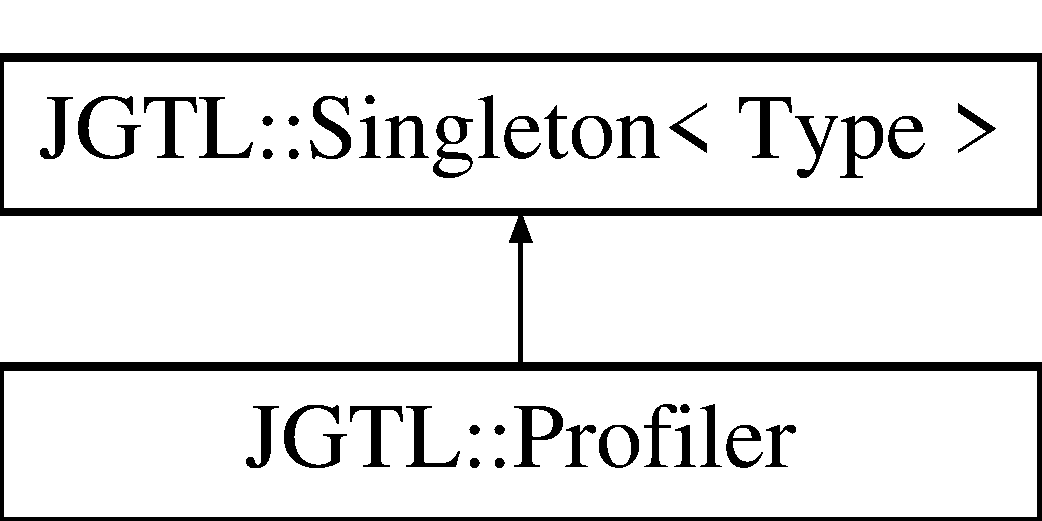
\includegraphics[height=2cm]{class_j_g_t_l_1_1_singleton}
\end{center}
\end{figure}
\subsection*{Static Public Member Functions}
\begin{CompactItemize}
\item 
static Type $\ast$ \hyperlink{class_j_g_t_l_1_1_singleton_ce18cf22abba60cac12ae26914ef3853}{get\-Instance} (void)
\item 
static void \hyperlink{class_j_g_t_l_1_1_singleton_59788c79ef7102b584b475aafc9e2315}{destroy\-Instance} ()
\end{CompactItemize}
\subsection*{Protected Member Functions}
\begin{CompactItemize}
\item 
\hyperlink{class_j_g_t_l_1_1_singleton_c7877acab4b56ed562f642e040247c7a}{Singleton} ()
\item 
virtual \hyperlink{class_j_g_t_l_1_1_singleton_44f0141a9d7e4931361ea08186c65300}{$\sim$Singleton} ()
\end{CompactItemize}
\subsection*{Static Protected Attributes}
\begin{CompactItemize}
\item 
static Type $\ast$ \hyperlink{class_j_g_t_l_1_1_singleton_a3be92cc77155d83555fbecc5469135b}{instance}
\end{CompactItemize}


\subsection{Detailed Description}
\subsubsection*{template$<$class Type$>$ class JGTL::Singleton$<$ Type $>$}

This class handles Singletons (Global Single-Instance Classes). 

\begin{Desc}
\item[Author:]Jason Gauci \end{Desc}
\begin{Desc}
\item[Date:]2008 \end{Desc}




\subsection{Constructor \& Destructor Documentation}
\hypertarget{class_j_g_t_l_1_1_singleton_c7877acab4b56ed562f642e040247c7a}{
\index{JGTL::Singleton@{JGTL::Singleton}!Singleton@{Singleton}}
\index{Singleton@{Singleton}!JGTL::Singleton@{JGTL::Singleton}}
\subsubsection[Singleton]{\setlength{\rightskip}{0pt plus 5cm}template$<$class Type$>$ \hyperlink{class_j_g_t_l_1_1_singleton}{JGTL::Singleton}$<$ Type $>$::\hyperlink{class_j_g_t_l_1_1_singleton}{Singleton} ()\hspace{0.3cm}{\tt  \mbox{[}inline, protected\mbox{]}}}}
\label{class_j_g_t_l_1_1_singleton_c7877acab4b56ed562f642e040247c7a}


\hypertarget{class_j_g_t_l_1_1_singleton_44f0141a9d7e4931361ea08186c65300}{
\index{JGTL::Singleton@{JGTL::Singleton}!~Singleton@{$\sim$Singleton}}
\index{~Singleton@{$\sim$Singleton}!JGTL::Singleton@{JGTL::Singleton}}
\subsubsection[$\sim$Singleton]{\setlength{\rightskip}{0pt plus 5cm}template$<$class Type$>$ virtual \hyperlink{class_j_g_t_l_1_1_singleton}{JGTL::Singleton}$<$ Type $>$::$\sim$\hyperlink{class_j_g_t_l_1_1_singleton}{Singleton} ()\hspace{0.3cm}{\tt  \mbox{[}inline, protected, virtual\mbox{]}}}}
\label{class_j_g_t_l_1_1_singleton_44f0141a9d7e4931361ea08186c65300}




\subsection{Member Function Documentation}
\hypertarget{class_j_g_t_l_1_1_singleton_ce18cf22abba60cac12ae26914ef3853}{
\index{JGTL::Singleton@{JGTL::Singleton}!getInstance@{getInstance}}
\index{getInstance@{getInstance}!JGTL::Singleton@{JGTL::Singleton}}
\subsubsection[getInstance]{\setlength{\rightskip}{0pt plus 5cm}template$<$class Type$>$ static Type$\ast$ \hyperlink{class_j_g_t_l_1_1_singleton}{JGTL::Singleton}$<$ Type $>$::get\-Instance (void)\hspace{0.3cm}{\tt  \mbox{[}inline, static\mbox{]}}}}
\label{class_j_g_t_l_1_1_singleton_ce18cf22abba60cac12ae26914ef3853}


\hypertarget{class_j_g_t_l_1_1_singleton_59788c79ef7102b584b475aafc9e2315}{
\index{JGTL::Singleton@{JGTL::Singleton}!destroyInstance@{destroyInstance}}
\index{destroyInstance@{destroyInstance}!JGTL::Singleton@{JGTL::Singleton}}
\subsubsection[destroyInstance]{\setlength{\rightskip}{0pt plus 5cm}template$<$class Type$>$ static void \hyperlink{class_j_g_t_l_1_1_singleton}{JGTL::Singleton}$<$ Type $>$::destroy\-Instance ()\hspace{0.3cm}{\tt  \mbox{[}inline, static\mbox{]}}}}
\label{class_j_g_t_l_1_1_singleton_59788c79ef7102b584b475aafc9e2315}




Reimplemented in \hyperlink{class_j_g_t_l_1_1_profiler_cb990d68355312b6cd7a1f494e4dd33c}{JGTL::Profiler}.

\subsection{Member Data Documentation}
\hypertarget{class_j_g_t_l_1_1_singleton_a3be92cc77155d83555fbecc5469135b}{
\index{JGTL::Singleton@{JGTL::Singleton}!instance@{instance}}
\index{instance@{instance}!JGTL::Singleton@{JGTL::Singleton}}
\subsubsection[instance]{\setlength{\rightskip}{0pt plus 5cm}template$<$class Type$>$ Type $\ast$ \hyperlink{class_j_g_t_l_1_1_singleton}{JGTL::Singleton}$<$ Type $>$::\hyperlink{class_j_g_t_l_1_1_singleton_a3be92cc77155d83555fbecc5469135b}{instance}\hspace{0.3cm}{\tt  \mbox{[}static, protected\mbox{]}}}}
\label{class_j_g_t_l_1_1_singleton_a3be92cc77155d83555fbecc5469135b}




The documentation for this class was generated from the following file:\begin{CompactItemize}
\item 
\hyperlink{_j_g_t_l___singleton_8h}{JGTL\_\-Singleton.h}\end{CompactItemize}

\hypertarget{class_j_g_t_l_1_1_sorted_list}{
\section{JGTL::Sorted\-List$<$ Data $>$ Class Template Reference}
\label{class_j_g_t_l_1_1_sorted_list}\index{JGTL::SortedList@{JGTL::SortedList}}
}
{\tt \#include $<$JGTL\_\-Sorted\-List\_\-delete.h$>$}

\subsection*{Public Member Functions}
\begin{CompactItemize}
\item 
\hyperlink{class_j_g_t_l_1_1_sorted_list_1aeb5755a4b248591c707fcb1ff27052}{Sorted\-List} (size\_\-t \_\-max\-Elements)
\item 
virtual \hyperlink{class_j_g_t_l_1_1_sorted_list_a8556bcb4bec9a7819f673792c3bc03f}{$\sim$Sorted\-List} ()
\item 
void \hyperlink{class_j_g_t_l_1_1_sorted_list_374a692e9fc1fe007d2c3d7471731fc1}{add\-Data} (const Data \&data)
\item 
const size\_\-t \& \hyperlink{class_j_g_t_l_1_1_sorted_list_a91c989bf22b3ac5d25c00f5a36389c5}{get\-Data\-Size} ()
\item 
const bool \hyperlink{class_j_g_t_l_1_1_sorted_list_8acf88bdfe7f74a11e4c2dc945ec165d}{has\-Data} (const Data \&other) const 
\item 
const Data \& \hyperlink{class_j_g_t_l_1_1_sorted_list_2c2b54845e1d3fb62c70e2a60c322b35}{get\-Data} (size\_\-t index) const
\item 
const Data $\ast$ \hyperlink{class_j_g_t_l_1_1_sorted_list_c5d2b01457f3769e028afd5343685082}{get\-Data\-Ptr} (size\_\-t index) const
\end{CompactItemize}
\subsection*{Protected Attributes}
\begin{CompactItemize}
\item 
size\_\-t \hyperlink{class_j_g_t_l_1_1_sorted_list_69b46609908f5d677486ed01749ce515}{num\-Elements}
\item 
size\_\-t \hyperlink{class_j_g_t_l_1_1_sorted_list_263ce05febec35a732661d2c26acb3a3}{max\-Elements}
\item 
Data $\ast$ \hyperlink{class_j_g_t_l_1_1_sorted_list_8315e6bbcf773663fd19c5e369a78b2f}{data\-List}
\end{CompactItemize}
\subsubsection*{template$<$class Data$>$ class JGTL::Sorted\-List$<$ Data $>$}



\subsection{Constructor \& Destructor Documentation}
\hypertarget{class_j_g_t_l_1_1_sorted_list_1aeb5755a4b248591c707fcb1ff27052}{
\index{JGTL::SortedList@{JGTL::Sorted\-List}!SortedList@{SortedList}}
\index{SortedList@{SortedList}!JGTL::SortedList@{JGTL::Sorted\-List}}
\subsubsection[SortedList]{\setlength{\rightskip}{0pt plus 5cm}template$<$class Data$>$ \hyperlink{class_j_g_t_l_1_1_sorted_list}{JGTL::Sorted\-List}$<$ Data $>$::\hyperlink{class_j_g_t_l_1_1_sorted_list}{Sorted\-List} (size\_\-t {\em \_\-max\-Elements})\hspace{0.3cm}{\tt  \mbox{[}inline\mbox{]}}}}
\label{class_j_g_t_l_1_1_sorted_list_1aeb5755a4b248591c707fcb1ff27052}


\hypertarget{class_j_g_t_l_1_1_sorted_list_a8556bcb4bec9a7819f673792c3bc03f}{
\index{JGTL::SortedList@{JGTL::Sorted\-List}!~SortedList@{$\sim$SortedList}}
\index{~SortedList@{$\sim$SortedList}!JGTL::SortedList@{JGTL::Sorted\-List}}
\subsubsection[$\sim$SortedList]{\setlength{\rightskip}{0pt plus 5cm}template$<$class Data$>$ virtual \hyperlink{class_j_g_t_l_1_1_sorted_list}{JGTL::Sorted\-List}$<$ Data $>$::$\sim$\hyperlink{class_j_g_t_l_1_1_sorted_list}{Sorted\-List} ()\hspace{0.3cm}{\tt  \mbox{[}inline, virtual\mbox{]}}}}
\label{class_j_g_t_l_1_1_sorted_list_a8556bcb4bec9a7819f673792c3bc03f}




\subsection{Member Function Documentation}
\hypertarget{class_j_g_t_l_1_1_sorted_list_374a692e9fc1fe007d2c3d7471731fc1}{
\index{JGTL::SortedList@{JGTL::Sorted\-List}!addData@{addData}}
\index{addData@{addData}!JGTL::SortedList@{JGTL::Sorted\-List}}
\subsubsection[addData]{\setlength{\rightskip}{0pt plus 5cm}template$<$class Data$>$ void \hyperlink{class_j_g_t_l_1_1_sorted_list}{JGTL::Sorted\-List}$<$ Data $>$::add\-Data (const Data \& {\em data})\hspace{0.3cm}{\tt  \mbox{[}inline\mbox{]}}}}
\label{class_j_g_t_l_1_1_sorted_list_374a692e9fc1fe007d2c3d7471731fc1}


\hypertarget{class_j_g_t_l_1_1_sorted_list_a91c989bf22b3ac5d25c00f5a36389c5}{
\index{JGTL::SortedList@{JGTL::Sorted\-List}!getDataSize@{getDataSize}}
\index{getDataSize@{getDataSize}!JGTL::SortedList@{JGTL::Sorted\-List}}
\subsubsection[getDataSize]{\setlength{\rightskip}{0pt plus 5cm}template$<$class Data$>$ const size\_\-t\& \hyperlink{class_j_g_t_l_1_1_sorted_list}{JGTL::Sorted\-List}$<$ Data $>$::get\-Data\-Size ()\hspace{0.3cm}{\tt  \mbox{[}inline\mbox{]}}}}
\label{class_j_g_t_l_1_1_sorted_list_a91c989bf22b3ac5d25c00f5a36389c5}


\hypertarget{class_j_g_t_l_1_1_sorted_list_8acf88bdfe7f74a11e4c2dc945ec165d}{
\index{JGTL::SortedList@{JGTL::Sorted\-List}!hasData@{hasData}}
\index{hasData@{hasData}!JGTL::SortedList@{JGTL::Sorted\-List}}
\subsubsection[hasData]{\setlength{\rightskip}{0pt plus 5cm}template$<$class Data$>$ const bool \hyperlink{class_j_g_t_l_1_1_sorted_list}{JGTL::Sorted\-List}$<$ Data $>$::has\-Data (const Data \& {\em other}) const\hspace{0.3cm}{\tt  \mbox{[}inline\mbox{]}}}}
\label{class_j_g_t_l_1_1_sorted_list_8acf88bdfe7f74a11e4c2dc945ec165d}


\hypertarget{class_j_g_t_l_1_1_sorted_list_2c2b54845e1d3fb62c70e2a60c322b35}{
\index{JGTL::SortedList@{JGTL::Sorted\-List}!getData@{getData}}
\index{getData@{getData}!JGTL::SortedList@{JGTL::Sorted\-List}}
\subsubsection[getData]{\setlength{\rightskip}{0pt plus 5cm}template$<$class Data$>$ const Data\& \hyperlink{class_j_g_t_l_1_1_sorted_list}{JGTL::Sorted\-List}$<$ Data $>$::get\-Data (size\_\-t {\em index}) const\hspace{0.3cm}{\tt  \mbox{[}inline\mbox{]}}}}
\label{class_j_g_t_l_1_1_sorted_list_2c2b54845e1d3fb62c70e2a60c322b35}


\hypertarget{class_j_g_t_l_1_1_sorted_list_c5d2b01457f3769e028afd5343685082}{
\index{JGTL::SortedList@{JGTL::Sorted\-List}!getDataPtr@{getDataPtr}}
\index{getDataPtr@{getDataPtr}!JGTL::SortedList@{JGTL::Sorted\-List}}
\subsubsection[getDataPtr]{\setlength{\rightskip}{0pt plus 5cm}template$<$class Data$>$ const Data$\ast$ \hyperlink{class_j_g_t_l_1_1_sorted_list}{JGTL::Sorted\-List}$<$ Data $>$::get\-Data\-Ptr (size\_\-t {\em index}) const\hspace{0.3cm}{\tt  \mbox{[}inline\mbox{]}}}}
\label{class_j_g_t_l_1_1_sorted_list_c5d2b01457f3769e028afd5343685082}




\subsection{Member Data Documentation}
\hypertarget{class_j_g_t_l_1_1_sorted_list_69b46609908f5d677486ed01749ce515}{
\index{JGTL::SortedList@{JGTL::Sorted\-List}!numElements@{numElements}}
\index{numElements@{numElements}!JGTL::SortedList@{JGTL::Sorted\-List}}
\subsubsection[numElements]{\setlength{\rightskip}{0pt plus 5cm}template$<$class Data$>$ size\_\-t \hyperlink{class_j_g_t_l_1_1_sorted_list}{JGTL::Sorted\-List}$<$ Data $>$::\hyperlink{class_j_g_t_l_1_1_sorted_list_69b46609908f5d677486ed01749ce515}{num\-Elements}\hspace{0.3cm}{\tt  \mbox{[}protected\mbox{]}}}}
\label{class_j_g_t_l_1_1_sorted_list_69b46609908f5d677486ed01749ce515}


\hypertarget{class_j_g_t_l_1_1_sorted_list_263ce05febec35a732661d2c26acb3a3}{
\index{JGTL::SortedList@{JGTL::Sorted\-List}!maxElements@{maxElements}}
\index{maxElements@{maxElements}!JGTL::SortedList@{JGTL::Sorted\-List}}
\subsubsection[maxElements]{\setlength{\rightskip}{0pt plus 5cm}template$<$class Data$>$ size\_\-t \hyperlink{class_j_g_t_l_1_1_sorted_list}{JGTL::Sorted\-List}$<$ Data $>$::\hyperlink{class_j_g_t_l_1_1_sorted_list_263ce05febec35a732661d2c26acb3a3}{max\-Elements}\hspace{0.3cm}{\tt  \mbox{[}protected\mbox{]}}}}
\label{class_j_g_t_l_1_1_sorted_list_263ce05febec35a732661d2c26acb3a3}


\hypertarget{class_j_g_t_l_1_1_sorted_list_8315e6bbcf773663fd19c5e369a78b2f}{
\index{JGTL::SortedList@{JGTL::Sorted\-List}!dataList@{dataList}}
\index{dataList@{dataList}!JGTL::SortedList@{JGTL::Sorted\-List}}
\subsubsection[dataList]{\setlength{\rightskip}{0pt plus 5cm}template$<$class Data$>$ Data$\ast$ \hyperlink{class_j_g_t_l_1_1_sorted_list}{JGTL::Sorted\-List}$<$ Data $>$::\hyperlink{class_j_g_t_l_1_1_sorted_list_8315e6bbcf773663fd19c5e369a78b2f}{data\-List}\hspace{0.3cm}{\tt  \mbox{[}protected\mbox{]}}}}
\label{class_j_g_t_l_1_1_sorted_list_8315e6bbcf773663fd19c5e369a78b2f}




The documentation for this class was generated from the following file:\begin{CompactItemize}
\item 
\hyperlink{_j_g_t_l___sorted_list__delete_8h}{JGTL\_\-Sorted\-List\_\-delete.h}\end{CompactItemize}

\hypertarget{class_j_g_t_l_1_1_stack_circular_buffer}{
\section{JGTL::Stack\-Circular\-Buffer$<$ Data, MAX\_\-ELEMENTS $>$ Class Template Reference}
\label{class_j_g_t_l_1_1_stack_circular_buffer}\index{JGTL::StackCircularBuffer@{JGTL::StackCircularBuffer}}
}
The \hyperlink{class_j_g_t_l_1_1_stack_circular_buffer}{Stack\-Circular\-Buffer} Class handles a Circular Buffer.  


{\tt \#include $<$JGTL\_\-Stack\-Circular\-Buffer.h$>$}

Inheritance diagram for JGTL::Stack\-Circular\-Buffer$<$ Data, MAX\_\-ELEMENTS $>$::\begin{figure}[H]
\begin{center}
\leavevmode
\includegraphics[height=2cm]{class_j_g_t_l_1_1_stack_circular_buffer}
\end{center}
\end{figure}
\subsection*{Public Member Functions}
\begin{CompactItemize}
\item 
\hyperlink{class_j_g_t_l_1_1_stack_circular_buffer_7c4eab48cf58e51095ae649a2ca1ac80}{Stack\-Circular\-Buffer} ()
\item 
\hyperlink{class_j_g_t_l_1_1_stack_circular_buffer_5446118506dc4721fcb96a6ede231c26}{Stack\-Circular\-Buffer} (const \hyperlink{class_j_g_t_l_1_1_stack_circular_buffer}{Stack\-Circular\-Buffer} \&other)
\item 
const \hyperlink{class_j_g_t_l_1_1_stack_circular_buffer}{Stack\-Circular\-Buffer} \& \hyperlink{class_j_g_t_l_1_1_stack_circular_buffer_1a099357e861a7baa232b3ee3ecbd6f4}{operator=} (const \hyperlink{class_j_g_t_l_1_1_stack_circular_buffer}{Stack\-Circular\-Buffer} \&other)
\item 
virtual \hyperlink{class_j_g_t_l_1_1_stack_circular_buffer_68a5c68dcf1b7d30bfc0c5b90db6fdcd}{$\sim$Stack\-Circular\-Buffer} ()
\item 
virtual bool \hyperlink{class_j_g_t_l_1_1_stack_circular_buffer_07b33fe01ef78d42d06a2cce77ffd2be}{resize} (int new\-Size)
\end{CompactItemize}
\subsection*{Protected Member Functions}
\begin{CompactItemize}
\item 
void \hyperlink{class_j_g_t_l_1_1_stack_circular_buffer_e5e4f039f4463be0f086d52bb262a314}{copy\-From} (const \hyperlink{class_j_g_t_l_1_1_stack_circular_buffer}{Stack\-Circular\-Buffer} \&other)
\end{CompactItemize}
\subsection*{Protected Attributes}
\begin{CompactItemize}
\item 
unsigned char \hyperlink{class_j_g_t_l_1_1_stack_circular_buffer_dd8559d1e2f47be8c10154768a997bfa}{data} \mbox{[}MAX\_\-ELEMENTS $\ast$sizeof(Data)\mbox{]}
\end{CompactItemize}


\subsection{Detailed Description}
\subsubsection*{template$<$class Data, int MAX\_\-ELEMENTS = 32$>$ class JGTL::Stack\-Circular\-Buffer$<$ Data, MAX\_\-ELEMENTS $>$}

The \hyperlink{class_j_g_t_l_1_1_stack_circular_buffer}{Stack\-Circular\-Buffer} Class handles a Circular Buffer. 

\begin{Desc}
\item[Author:]Jason Gauci \end{Desc}
\begin{Desc}
\item[Date:]2008 \end{Desc}




\subsection{Constructor \& Destructor Documentation}
\hypertarget{class_j_g_t_l_1_1_stack_circular_buffer_7c4eab48cf58e51095ae649a2ca1ac80}{
\index{JGTL::StackCircularBuffer@{JGTL::Stack\-Circular\-Buffer}!StackCircularBuffer@{StackCircularBuffer}}
\index{StackCircularBuffer@{StackCircularBuffer}!JGTL::StackCircularBuffer@{JGTL::Stack\-Circular\-Buffer}}
\subsubsection[StackCircularBuffer]{\setlength{\rightskip}{0pt plus 5cm}template$<$class Data, int MAX\_\-ELEMENTS = 32$>$ \hyperlink{class_j_g_t_l_1_1_stack_circular_buffer}{JGTL::Stack\-Circular\-Buffer}$<$ Data, MAX\_\-ELEMENTS $>$::\hyperlink{class_j_g_t_l_1_1_stack_circular_buffer}{Stack\-Circular\-Buffer} ()\hspace{0.3cm}{\tt  \mbox{[}inline\mbox{]}}}}
\label{class_j_g_t_l_1_1_stack_circular_buffer_7c4eab48cf58e51095ae649a2ca1ac80}


\hypertarget{class_j_g_t_l_1_1_stack_circular_buffer_5446118506dc4721fcb96a6ede231c26}{
\index{JGTL::StackCircularBuffer@{JGTL::Stack\-Circular\-Buffer}!StackCircularBuffer@{StackCircularBuffer}}
\index{StackCircularBuffer@{StackCircularBuffer}!JGTL::StackCircularBuffer@{JGTL::Stack\-Circular\-Buffer}}
\subsubsection[StackCircularBuffer]{\setlength{\rightskip}{0pt plus 5cm}template$<$class Data, int MAX\_\-ELEMENTS = 32$>$ \hyperlink{class_j_g_t_l_1_1_stack_circular_buffer}{JGTL::Stack\-Circular\-Buffer}$<$ Data, MAX\_\-ELEMENTS $>$::\hyperlink{class_j_g_t_l_1_1_stack_circular_buffer}{Stack\-Circular\-Buffer} (const \hyperlink{class_j_g_t_l_1_1_stack_circular_buffer}{Stack\-Circular\-Buffer}$<$ Data, MAX\_\-ELEMENTS $>$ \& {\em other})\hspace{0.3cm}{\tt  \mbox{[}inline\mbox{]}}}}
\label{class_j_g_t_l_1_1_stack_circular_buffer_5446118506dc4721fcb96a6ede231c26}


\hypertarget{class_j_g_t_l_1_1_stack_circular_buffer_68a5c68dcf1b7d30bfc0c5b90db6fdcd}{
\index{JGTL::StackCircularBuffer@{JGTL::Stack\-Circular\-Buffer}!~StackCircularBuffer@{$\sim$StackCircularBuffer}}
\index{~StackCircularBuffer@{$\sim$StackCircularBuffer}!JGTL::StackCircularBuffer@{JGTL::Stack\-Circular\-Buffer}}
\subsubsection[$\sim$StackCircularBuffer]{\setlength{\rightskip}{0pt plus 5cm}template$<$class Data, int MAX\_\-ELEMENTS = 32$>$ virtual \hyperlink{class_j_g_t_l_1_1_stack_circular_buffer}{JGTL::Stack\-Circular\-Buffer}$<$ Data, MAX\_\-ELEMENTS $>$::$\sim$\hyperlink{class_j_g_t_l_1_1_stack_circular_buffer}{Stack\-Circular\-Buffer} ()\hspace{0.3cm}{\tt  \mbox{[}inline, virtual\mbox{]}}}}
\label{class_j_g_t_l_1_1_stack_circular_buffer_68a5c68dcf1b7d30bfc0c5b90db6fdcd}




\subsection{Member Function Documentation}
\hypertarget{class_j_g_t_l_1_1_stack_circular_buffer_1a099357e861a7baa232b3ee3ecbd6f4}{
\index{JGTL::StackCircularBuffer@{JGTL::Stack\-Circular\-Buffer}!operator=@{operator=}}
\index{operator=@{operator=}!JGTL::StackCircularBuffer@{JGTL::Stack\-Circular\-Buffer}}
\subsubsection[operator=]{\setlength{\rightskip}{0pt plus 5cm}template$<$class Data, int MAX\_\-ELEMENTS = 32$>$ const \hyperlink{class_j_g_t_l_1_1_stack_circular_buffer}{Stack\-Circular\-Buffer}\& \hyperlink{class_j_g_t_l_1_1_stack_circular_buffer}{JGTL::Stack\-Circular\-Buffer}$<$ Data, MAX\_\-ELEMENTS $>$::operator= (const \hyperlink{class_j_g_t_l_1_1_stack_circular_buffer}{Stack\-Circular\-Buffer}$<$ Data, MAX\_\-ELEMENTS $>$ \& {\em other})\hspace{0.3cm}{\tt  \mbox{[}inline\mbox{]}}}}
\label{class_j_g_t_l_1_1_stack_circular_buffer_1a099357e861a7baa232b3ee3ecbd6f4}


\hypertarget{class_j_g_t_l_1_1_stack_circular_buffer_07b33fe01ef78d42d06a2cce77ffd2be}{
\index{JGTL::StackCircularBuffer@{JGTL::Stack\-Circular\-Buffer}!resize@{resize}}
\index{resize@{resize}!JGTL::StackCircularBuffer@{JGTL::Stack\-Circular\-Buffer}}
\subsubsection[resize]{\setlength{\rightskip}{0pt plus 5cm}template$<$class Data, int MAX\_\-ELEMENTS = 32$>$ virtual bool \hyperlink{class_j_g_t_l_1_1_stack_circular_buffer}{JGTL::Stack\-Circular\-Buffer}$<$ Data, MAX\_\-ELEMENTS $>$::resize (int {\em new\-Size})\hspace{0.3cm}{\tt  \mbox{[}inline, virtual\mbox{]}}}}
\label{class_j_g_t_l_1_1_stack_circular_buffer_07b33fe01ef78d42d06a2cce77ffd2be}




Implements \hyperlink{class_j_g_t_l_1_1_circular_buffer_interface_c6976a1811fdeb5b1810e379022f67ba}{JGTL::Circular\-Buffer\-Interface$<$ Data $>$}.\hypertarget{class_j_g_t_l_1_1_stack_circular_buffer_e5e4f039f4463be0f086d52bb262a314}{
\index{JGTL::StackCircularBuffer@{JGTL::Stack\-Circular\-Buffer}!copyFrom@{copyFrom}}
\index{copyFrom@{copyFrom}!JGTL::StackCircularBuffer@{JGTL::Stack\-Circular\-Buffer}}
\subsubsection[copyFrom]{\setlength{\rightskip}{0pt plus 5cm}template$<$class Data, int MAX\_\-ELEMENTS = 32$>$ void \hyperlink{class_j_g_t_l_1_1_stack_circular_buffer}{JGTL::Stack\-Circular\-Buffer}$<$ Data, MAX\_\-ELEMENTS $>$::copy\-From (const \hyperlink{class_j_g_t_l_1_1_stack_circular_buffer}{Stack\-Circular\-Buffer}$<$ Data, MAX\_\-ELEMENTS $>$ \& {\em other})\hspace{0.3cm}{\tt  \mbox{[}inline, protected\mbox{]}}}}
\label{class_j_g_t_l_1_1_stack_circular_buffer_e5e4f039f4463be0f086d52bb262a314}




\subsection{Member Data Documentation}
\hypertarget{class_j_g_t_l_1_1_stack_circular_buffer_dd8559d1e2f47be8c10154768a997bfa}{
\index{JGTL::StackCircularBuffer@{JGTL::Stack\-Circular\-Buffer}!data@{data}}
\index{data@{data}!JGTL::StackCircularBuffer@{JGTL::Stack\-Circular\-Buffer}}
\subsubsection[data]{\setlength{\rightskip}{0pt plus 5cm}template$<$class Data, int MAX\_\-ELEMENTS = 32$>$ unsigned char \hyperlink{class_j_g_t_l_1_1_stack_circular_buffer}{JGTL::Stack\-Circular\-Buffer}$<$ Data, MAX\_\-ELEMENTS $>$::\hyperlink{class_j_g_t_l_1_1_stack_circular_buffer_dd8559d1e2f47be8c10154768a997bfa}{data}\mbox{[}MAX\_\-ELEMENTS $\ast$sizeof(Data)\mbox{]}\hspace{0.3cm}{\tt  \mbox{[}protected\mbox{]}}}}
\label{class_j_g_t_l_1_1_stack_circular_buffer_dd8559d1e2f47be8c10154768a997bfa}




The documentation for this class was generated from the following file:\begin{CompactItemize}
\item 
\hyperlink{_j_g_t_l___stack_circular_buffer_8h}{JGTL\_\-Stack\-Circular\-Buffer.h}\end{CompactItemize}

\hypertarget{class_j_g_t_l_1_1_stack_map}{
\section{JGTL::Stack\-Map$<$ Key, Data, MAX\_\-ELEMENTS $>$ Class Template Reference}
\label{class_j_g_t_l_1_1_stack_map}\index{JGTL::StackMap@{JGTL::StackMap}}
}
The \hyperlink{class_j_g_t_l_1_1_stack_map}{Stack\-Map} Class is a fixed, array-based, sorted key structure.  


{\tt \#include $<$JGTL\_\-Stack\-Map.h$>$}

Inheritance diagram for JGTL::Stack\-Map$<$ Key, Data, MAX\_\-ELEMENTS $>$::\begin{figure}[H]
\begin{center}
\leavevmode
\includegraphics[height=2cm]{class_j_g_t_l_1_1_stack_map}
\end{center}
\end{figure}
\subsection*{Public Member Functions}
\begin{CompactItemize}
\item 
\hyperlink{class_j_g_t_l_1_1_stack_map_e6cb52e89d332a1438fa0b807081c46a}{Stack\-Map} ()
\item 
\hyperlink{class_j_g_t_l_1_1_stack_map_a51a9f733e87c5da70660b73e8cf9651}{Stack\-Map} (const \hyperlink{class_j_g_t_l_1_1_stack_map}{Stack\-Map} \&other)
\item 
const \hyperlink{class_j_g_t_l_1_1_stack_map}{Stack\-Map} \& \hyperlink{class_j_g_t_l_1_1_stack_map_5e2b185fcda84ac8a692bd57159d97e9}{operator=} (const \hyperlink{class_j_g_t_l_1_1_stack_map}{Stack\-Map} \&other)
\item 
virtual \hyperlink{class_j_g_t_l_1_1_stack_map_e1648b2a04c3b9d57cb2377bcc8f94a8}{$\sim$Stack\-Map} ()
\item 
virtual bool \hyperlink{class_j_g_t_l_1_1_stack_map_cd9363efffeb00f6b48b21ed2685ac7c}{resize} (int new\-Size)
\end{CompactItemize}
\subsection*{Protected Member Functions}
\begin{CompactItemize}
\item 
virtual void \hyperlink{class_j_g_t_l_1_1_stack_map_3475bde07f081d0c7bbf821703c6f099}{copy\-From} (const \hyperlink{class_j_g_t_l_1_1_stack_map}{Stack\-Map} \&other)
\end{CompactItemize}
\subsection*{Protected Attributes}
\begin{CompactItemize}
\item 
unsigned char \hyperlink{class_j_g_t_l_1_1_stack_map_9a3cc307f2892b669714253d75792e2e}{data} \mbox{[}MAX\_\-ELEMENTS $\ast$sizeof(std::pair$<$ Key, Data $>$)\mbox{]}
\end{CompactItemize}


\subsection{Detailed Description}
\subsubsection*{template$<$class Key, class Data, int MAX\_\-ELEMENTS = 8$>$ class JGTL::Stack\-Map$<$ Key, Data, MAX\_\-ELEMENTS $>$}

The \hyperlink{class_j_g_t_l_1_1_stack_map}{Stack\-Map} Class is a fixed, array-based, sorted key structure. 

\begin{Desc}
\item[Author:]Jason Gauci \end{Desc}
\begin{Desc}
\item[Date:]2008 \end{Desc}




\subsection{Constructor \& Destructor Documentation}
\hypertarget{class_j_g_t_l_1_1_stack_map_e6cb52e89d332a1438fa0b807081c46a}{
\index{JGTL::StackMap@{JGTL::Stack\-Map}!StackMap@{StackMap}}
\index{StackMap@{StackMap}!JGTL::StackMap@{JGTL::Stack\-Map}}
\subsubsection[StackMap]{\setlength{\rightskip}{0pt plus 5cm}template$<$class Key, class Data, int MAX\_\-ELEMENTS = 8$>$ \hyperlink{class_j_g_t_l_1_1_stack_map}{JGTL::Stack\-Map}$<$ Key, Data, MAX\_\-ELEMENTS $>$::\hyperlink{class_j_g_t_l_1_1_stack_map}{Stack\-Map} ()\hspace{0.3cm}{\tt  \mbox{[}inline\mbox{]}}}}
\label{class_j_g_t_l_1_1_stack_map_e6cb52e89d332a1438fa0b807081c46a}


\hypertarget{class_j_g_t_l_1_1_stack_map_a51a9f733e87c5da70660b73e8cf9651}{
\index{JGTL::StackMap@{JGTL::Stack\-Map}!StackMap@{StackMap}}
\index{StackMap@{StackMap}!JGTL::StackMap@{JGTL::Stack\-Map}}
\subsubsection[StackMap]{\setlength{\rightskip}{0pt plus 5cm}template$<$class Key, class Data, int MAX\_\-ELEMENTS = 8$>$ \hyperlink{class_j_g_t_l_1_1_stack_map}{JGTL::Stack\-Map}$<$ Key, Data, MAX\_\-ELEMENTS $>$::\hyperlink{class_j_g_t_l_1_1_stack_map}{Stack\-Map} (const \hyperlink{class_j_g_t_l_1_1_stack_map}{Stack\-Map}$<$ Key, Data, MAX\_\-ELEMENTS $>$ \& {\em other})\hspace{0.3cm}{\tt  \mbox{[}inline\mbox{]}}}}
\label{class_j_g_t_l_1_1_stack_map_a51a9f733e87c5da70660b73e8cf9651}


\hypertarget{class_j_g_t_l_1_1_stack_map_e1648b2a04c3b9d57cb2377bcc8f94a8}{
\index{JGTL::StackMap@{JGTL::Stack\-Map}!~StackMap@{$\sim$StackMap}}
\index{~StackMap@{$\sim$StackMap}!JGTL::StackMap@{JGTL::Stack\-Map}}
\subsubsection[$\sim$StackMap]{\setlength{\rightskip}{0pt plus 5cm}template$<$class Key, class Data, int MAX\_\-ELEMENTS = 8$>$ virtual \hyperlink{class_j_g_t_l_1_1_stack_map}{JGTL::Stack\-Map}$<$ Key, Data, MAX\_\-ELEMENTS $>$::$\sim$\hyperlink{class_j_g_t_l_1_1_stack_map}{Stack\-Map} ()\hspace{0.3cm}{\tt  \mbox{[}inline, virtual\mbox{]}}}}
\label{class_j_g_t_l_1_1_stack_map_e1648b2a04c3b9d57cb2377bcc8f94a8}




\subsection{Member Function Documentation}
\hypertarget{class_j_g_t_l_1_1_stack_map_5e2b185fcda84ac8a692bd57159d97e9}{
\index{JGTL::StackMap@{JGTL::Stack\-Map}!operator=@{operator=}}
\index{operator=@{operator=}!JGTL::StackMap@{JGTL::Stack\-Map}}
\subsubsection[operator=]{\setlength{\rightskip}{0pt plus 5cm}template$<$class Key, class Data, int MAX\_\-ELEMENTS = 8$>$ const \hyperlink{class_j_g_t_l_1_1_stack_map}{Stack\-Map}\& \hyperlink{class_j_g_t_l_1_1_stack_map}{JGTL::Stack\-Map}$<$ Key, Data, MAX\_\-ELEMENTS $>$::operator= (const \hyperlink{class_j_g_t_l_1_1_stack_map}{Stack\-Map}$<$ Key, Data, MAX\_\-ELEMENTS $>$ \& {\em other})\hspace{0.3cm}{\tt  \mbox{[}inline\mbox{]}}}}
\label{class_j_g_t_l_1_1_stack_map_5e2b185fcda84ac8a692bd57159d97e9}


\hypertarget{class_j_g_t_l_1_1_stack_map_cd9363efffeb00f6b48b21ed2685ac7c}{
\index{JGTL::StackMap@{JGTL::Stack\-Map}!resize@{resize}}
\index{resize@{resize}!JGTL::StackMap@{JGTL::Stack\-Map}}
\subsubsection[resize]{\setlength{\rightskip}{0pt plus 5cm}template$<$class Key, class Data, int MAX\_\-ELEMENTS = 8$>$ virtual bool \hyperlink{class_j_g_t_l_1_1_stack_map}{JGTL::Stack\-Map}$<$ Key, Data, MAX\_\-ELEMENTS $>$::resize (int {\em new\-Size})\hspace{0.3cm}{\tt  \mbox{[}inline, virtual\mbox{]}}}}
\label{class_j_g_t_l_1_1_stack_map_cd9363efffeb00f6b48b21ed2685ac7c}




Implements \hyperlink{class_j_g_t_l_1_1_map_interface_177b75de36104c54e53080db65b777a2}{JGTL::Map\-Interface$<$ Key, Data $>$}.\hypertarget{class_j_g_t_l_1_1_stack_map_3475bde07f081d0c7bbf821703c6f099}{
\index{JGTL::StackMap@{JGTL::Stack\-Map}!copyFrom@{copyFrom}}
\index{copyFrom@{copyFrom}!JGTL::StackMap@{JGTL::Stack\-Map}}
\subsubsection[copyFrom]{\setlength{\rightskip}{0pt plus 5cm}template$<$class Key, class Data, int MAX\_\-ELEMENTS = 8$>$ virtual void \hyperlink{class_j_g_t_l_1_1_stack_map}{JGTL::Stack\-Map}$<$ Key, Data, MAX\_\-ELEMENTS $>$::copy\-From (const \hyperlink{class_j_g_t_l_1_1_stack_map}{Stack\-Map}$<$ Key, Data, MAX\_\-ELEMENTS $>$ \& {\em other})\hspace{0.3cm}{\tt  \mbox{[}inline, protected, virtual\mbox{]}}}}
\label{class_j_g_t_l_1_1_stack_map_3475bde07f081d0c7bbf821703c6f099}




\subsection{Member Data Documentation}
\hypertarget{class_j_g_t_l_1_1_stack_map_9a3cc307f2892b669714253d75792e2e}{
\index{JGTL::StackMap@{JGTL::Stack\-Map}!data@{data}}
\index{data@{data}!JGTL::StackMap@{JGTL::Stack\-Map}}
\subsubsection[data]{\setlength{\rightskip}{0pt plus 5cm}template$<$class Key, class Data, int MAX\_\-ELEMENTS = 8$>$ unsigned char \hyperlink{class_j_g_t_l_1_1_stack_map}{JGTL::Stack\-Map}$<$ Key, Data, MAX\_\-ELEMENTS $>$::\hyperlink{class_j_g_t_l_1_1_stack_map_9a3cc307f2892b669714253d75792e2e}{data}\mbox{[}MAX\_\-ELEMENTS $\ast$sizeof(std::pair$<$ Key, Data $>$)\mbox{]}\hspace{0.3cm}{\tt  \mbox{[}protected\mbox{]}}}}
\label{class_j_g_t_l_1_1_stack_map_9a3cc307f2892b669714253d75792e2e}




The documentation for this class was generated from the following file:\begin{CompactItemize}
\item 
\hyperlink{_j_g_t_l___stack_map_8h}{JGTL\_\-Stack\-Map.h}\end{CompactItemize}

\hypertarget{class_j_g_t_l_1_1_stack_set}{
\section{JGTL::Stack\-Set$<$ Data, MAX\_\-ELEMENTS $>$ Class Template Reference}
\label{class_j_g_t_l_1_1_stack_set}\index{JGTL::StackSet@{JGTL::StackSet}}
}
{\tt \#include $<$JGTL\_\-Stack\-Set.h$>$}

Inheritance diagram for JGTL::Stack\-Set$<$ Data, MAX\_\-ELEMENTS $>$::\begin{figure}[H]
\begin{center}
\leavevmode
\includegraphics[height=2cm]{class_j_g_t_l_1_1_stack_set}
\end{center}
\end{figure}
\subsection*{Public Member Functions}
\begin{CompactItemize}
\item 
\hyperlink{class_j_g_t_l_1_1_stack_set_842b6b0d43ade3636a6f5eb7cc29cfc5}{Stack\-Set} ()
\item 
\hyperlink{class_j_g_t_l_1_1_stack_set_b2cc18e5b25781be9e000c3d206bfcbd}{Stack\-Set} (const \hyperlink{class_j_g_t_l_1_1_stack_set}{Stack\-Set} \&other)
\item 
const \hyperlink{class_j_g_t_l_1_1_stack_set}{Stack\-Set} \& \hyperlink{class_j_g_t_l_1_1_stack_set_6afeb5e3f6d4433b9938f3743f02aa1c}{operator=} (const \hyperlink{class_j_g_t_l_1_1_stack_set}{Stack\-Set} \&other)
\item 
virtual void \hyperlink{class_j_g_t_l_1_1_stack_set_0f724177e6688d06eb8c4923e225e82f}{copy\-From} (const \hyperlink{class_j_g_t_l_1_1_stack_set}{Stack\-Set} \&other)
\item 
virtual \hyperlink{class_j_g_t_l_1_1_stack_set_6494c9bbda6ab35af078faafaac7f02c}{$\sim$Stack\-Set} ()
\end{CompactItemize}
\subsection*{Protected Attributes}
\begin{CompactItemize}
\item 
unsigned char \hyperlink{class_j_g_t_l_1_1_stack_set_1c9f174be3aa9681935d4b7a300dbd79}{data} \mbox{[}MAX\_\-ELEMENTS $\ast$sizeof(Data)\mbox{]}
\end{CompactItemize}
\subsubsection*{template$<$class Data, int MAX\_\-ELEMENTS = 8$>$ class JGTL::Stack\-Set$<$ Data, MAX\_\-ELEMENTS $>$}



\subsection{Constructor \& Destructor Documentation}
\hypertarget{class_j_g_t_l_1_1_stack_set_842b6b0d43ade3636a6f5eb7cc29cfc5}{
\index{JGTL::StackSet@{JGTL::Stack\-Set}!StackSet@{StackSet}}
\index{StackSet@{StackSet}!JGTL::StackSet@{JGTL::Stack\-Set}}
\subsubsection[StackSet]{\setlength{\rightskip}{0pt plus 5cm}template$<$class Data, int MAX\_\-ELEMENTS = 8$>$ \hyperlink{class_j_g_t_l_1_1_stack_set}{JGTL::Stack\-Set}$<$ Data, MAX\_\-ELEMENTS $>$::\hyperlink{class_j_g_t_l_1_1_stack_set}{Stack\-Set} ()\hspace{0.3cm}{\tt  \mbox{[}inline\mbox{]}}}}
\label{class_j_g_t_l_1_1_stack_set_842b6b0d43ade3636a6f5eb7cc29cfc5}


\hypertarget{class_j_g_t_l_1_1_stack_set_b2cc18e5b25781be9e000c3d206bfcbd}{
\index{JGTL::StackSet@{JGTL::Stack\-Set}!StackSet@{StackSet}}
\index{StackSet@{StackSet}!JGTL::StackSet@{JGTL::Stack\-Set}}
\subsubsection[StackSet]{\setlength{\rightskip}{0pt plus 5cm}template$<$class Data, int MAX\_\-ELEMENTS = 8$>$ \hyperlink{class_j_g_t_l_1_1_stack_set}{JGTL::Stack\-Set}$<$ Data, MAX\_\-ELEMENTS $>$::\hyperlink{class_j_g_t_l_1_1_stack_set}{Stack\-Set} (const \hyperlink{class_j_g_t_l_1_1_stack_set}{Stack\-Set}$<$ Data, MAX\_\-ELEMENTS $>$ \& {\em other})\hspace{0.3cm}{\tt  \mbox{[}inline\mbox{]}}}}
\label{class_j_g_t_l_1_1_stack_set_b2cc18e5b25781be9e000c3d206bfcbd}


\hypertarget{class_j_g_t_l_1_1_stack_set_6494c9bbda6ab35af078faafaac7f02c}{
\index{JGTL::StackSet@{JGTL::Stack\-Set}!~StackSet@{$\sim$StackSet}}
\index{~StackSet@{$\sim$StackSet}!JGTL::StackSet@{JGTL::Stack\-Set}}
\subsubsection[$\sim$StackSet]{\setlength{\rightskip}{0pt plus 5cm}template$<$class Data, int MAX\_\-ELEMENTS = 8$>$ virtual \hyperlink{class_j_g_t_l_1_1_stack_set}{JGTL::Stack\-Set}$<$ Data, MAX\_\-ELEMENTS $>$::$\sim$\hyperlink{class_j_g_t_l_1_1_stack_set}{Stack\-Set} ()\hspace{0.3cm}{\tt  \mbox{[}inline, virtual\mbox{]}}}}
\label{class_j_g_t_l_1_1_stack_set_6494c9bbda6ab35af078faafaac7f02c}




\subsection{Member Function Documentation}
\hypertarget{class_j_g_t_l_1_1_stack_set_6afeb5e3f6d4433b9938f3743f02aa1c}{
\index{JGTL::StackSet@{JGTL::Stack\-Set}!operator=@{operator=}}
\index{operator=@{operator=}!JGTL::StackSet@{JGTL::Stack\-Set}}
\subsubsection[operator=]{\setlength{\rightskip}{0pt plus 5cm}template$<$class Data, int MAX\_\-ELEMENTS = 8$>$ const \hyperlink{class_j_g_t_l_1_1_stack_set}{Stack\-Set}\& \hyperlink{class_j_g_t_l_1_1_stack_set}{JGTL::Stack\-Set}$<$ Data, MAX\_\-ELEMENTS $>$::operator= (const \hyperlink{class_j_g_t_l_1_1_stack_set}{Stack\-Set}$<$ Data, MAX\_\-ELEMENTS $>$ \& {\em other})\hspace{0.3cm}{\tt  \mbox{[}inline\mbox{]}}}}
\label{class_j_g_t_l_1_1_stack_set_6afeb5e3f6d4433b9938f3743f02aa1c}


\hypertarget{class_j_g_t_l_1_1_stack_set_0f724177e6688d06eb8c4923e225e82f}{
\index{JGTL::StackSet@{JGTL::Stack\-Set}!copyFrom@{copyFrom}}
\index{copyFrom@{copyFrom}!JGTL::StackSet@{JGTL::Stack\-Set}}
\subsubsection[copyFrom]{\setlength{\rightskip}{0pt plus 5cm}template$<$class Data, int MAX\_\-ELEMENTS = 8$>$ virtual void \hyperlink{class_j_g_t_l_1_1_stack_set}{JGTL::Stack\-Set}$<$ Data, MAX\_\-ELEMENTS $>$::copy\-From (const \hyperlink{class_j_g_t_l_1_1_stack_set}{Stack\-Set}$<$ Data, MAX\_\-ELEMENTS $>$ \& {\em other})\hspace{0.3cm}{\tt  \mbox{[}inline, virtual\mbox{]}}}}
\label{class_j_g_t_l_1_1_stack_set_0f724177e6688d06eb8c4923e225e82f}




\subsection{Member Data Documentation}
\hypertarget{class_j_g_t_l_1_1_stack_set_1c9f174be3aa9681935d4b7a300dbd79}{
\index{JGTL::StackSet@{JGTL::Stack\-Set}!data@{data}}
\index{data@{data}!JGTL::StackSet@{JGTL::Stack\-Set}}
\subsubsection[data]{\setlength{\rightskip}{0pt plus 5cm}template$<$class Data, int MAX\_\-ELEMENTS = 8$>$ unsigned char \hyperlink{class_j_g_t_l_1_1_stack_set}{JGTL::Stack\-Set}$<$ Data, MAX\_\-ELEMENTS $>$::\hyperlink{class_j_g_t_l_1_1_stack_set_1c9f174be3aa9681935d4b7a300dbd79}{data}\mbox{[}MAX\_\-ELEMENTS $\ast$sizeof(Data)\mbox{]}\hspace{0.3cm}{\tt  \mbox{[}protected\mbox{]}}}}
\label{class_j_g_t_l_1_1_stack_set_1c9f174be3aa9681935d4b7a300dbd79}




The documentation for this class was generated from the following file:\begin{CompactItemize}
\item 
\hyperlink{_j_g_t_l___stack_set_8h}{JGTL\_\-Stack\-Set.h}\end{CompactItemize}

\hypertarget{struct_j_g_t_l_1_1_s_t_a_t_i_c___m_a_x___s_i_z_e}{
\section{JGTL::STATIC\_\-MAX\_\-SIZE$<$ One, Two, Three, Four, Five, Six, Seven, Eight, Nine, Ten $>$ Struct Template Reference}
\label{struct_j_g_t_l_1_1_s_t_a_t_i_c___m_a_x___s_i_z_e}\index{JGTL::STATIC_MAX_SIZE@{JGTL::STATIC\_\-MAX\_\-SIZE}}
}
{\tt \#include $<$JGTL\_\-Variant.h$>$}

\subsection*{Static Public Attributes}
\begin{CompactItemize}
\item 
static const int \hyperlink{struct_j_g_t_l_1_1_s_t_a_t_i_c___m_a_x___s_i_z_e_5976ed1e8db916f40b5dc6987ed095b8}{RESULT}
\end{CompactItemize}
\subsubsection*{template$<$class One, class Two = One, class Three = One, class Four = One, class Five = One, class Six = One, class Seven = One, class Eight = One, class Nine = One, class Ten = One$>$ struct JGTL::STATIC\_\-MAX\_\-SIZE$<$ One, Two, Three, Four, Five, Six, Seven, Eight, Nine, Ten $>$}



\subsection{Member Data Documentation}
\hypertarget{struct_j_g_t_l_1_1_s_t_a_t_i_c___m_a_x___s_i_z_e_5976ed1e8db916f40b5dc6987ed095b8}{
\index{JGTL::STATIC_MAX_SIZE@{JGTL::STATIC\_\-MAX\_\-SIZE}!RESULT@{RESULT}}
\index{RESULT@{RESULT}!JGTL::STATIC_MAX_SIZE@{JGTL::STATIC\_\-MAX\_\-SIZE}}
\subsubsection[RESULT]{\setlength{\rightskip}{0pt plus 5cm}template$<$class One, class Two = One, class Three = One, class Four = One, class Five = One, class Six = One, class Seven = One, class Eight = One, class Nine = One, class Ten = One$>$ const int \hyperlink{struct_j_g_t_l_1_1_s_t_a_t_i_c___m_a_x___s_i_z_e}{JGTL::STATIC\_\-MAX\_\-SIZE}$<$ One, Two, Three, Four, Five, Six, Seven, Eight, Nine, Ten $>$::\hyperlink{struct_j_g_t_l_1_1_s_t_a_t_i_c___m_a_x___s_i_z_e_5976ed1e8db916f40b5dc6987ed095b8}{RESULT}\hspace{0.3cm}{\tt  \mbox{[}static\mbox{]}}}}
\label{struct_j_g_t_l_1_1_s_t_a_t_i_c___m_a_x___s_i_z_e_5976ed1e8db916f40b5dc6987ed095b8}


\textbf{Initial value:}

\begin{Code}\begin{verbatim}
                        TYPEIF<
                        int,
                        (sizeof(Two) > sizeof(Three)),
                        STATIC_MAX_SIZE<One,One,Two,Four,Five,Six,Seven,Eight,Nine,Ten>::RESULT,
                        STATIC_MAX_SIZE<One,One,Three,Four,Five,Six,Seven,Eight,Nine,Ten>::RESULT
                        >::RESULT
\end{verbatim}\end{Code}


The documentation for this struct was generated from the following file:\begin{CompactItemize}
\item 
\hyperlink{_j_g_t_l___variant_8h}{JGTL\_\-Variant.h}\end{CompactItemize}

\hypertarget{struct_j_g_t_l_1_1_s_t_a_t_i_c___m_a_x___s_i_z_e_3_01_one_00_01_one_00_01_one_00_01_one_00_01_on8bad4fe85b3207b51b4ba282cb73273e}{
\section{JGTL::STATIC\_\-MAX\_\-SIZE$<$ One, One, One, One, One, One, One, One, One, Two $>$ Struct Template Reference}
\label{struct_j_g_t_l_1_1_s_t_a_t_i_c___m_a_x___s_i_z_e_3_01_one_00_01_one_00_01_one_00_01_one_00_01_on8bad4fe85b3207b51b4ba282cb73273e}\index{JGTL::STATIC_MAX_SIZE< One, One, One, One, One, One, One, One, One, Two >@{JGTL::STATIC\_\-MAX\_\-SIZE$<$ One, One, One, One, One, One, One, One, One, Two $>$}}
}
{\tt \#include $<$JGTL\_\-Variant.h$>$}

\subsection*{Static Public Attributes}
\begin{CompactItemize}
\item 
static const int \hyperlink{struct_j_g_t_l_1_1_s_t_a_t_i_c___m_a_x___s_i_z_e_3_01_one_00_01_one_00_01_one_00_01_one_00_01_on8bad4fe85b3207b51b4ba282cb73273e_5b5ccc194f236604d77f475aacbf3405}{RESULT}
\end{CompactItemize}
\subsubsection*{template$<$class One, class Two$>$ struct JGTL::STATIC\_\-MAX\_\-SIZE$<$ One, One, One, One, One, One, One, One, One, Two $>$}



\subsection{Member Data Documentation}
\hypertarget{struct_j_g_t_l_1_1_s_t_a_t_i_c___m_a_x___s_i_z_e_3_01_one_00_01_one_00_01_one_00_01_one_00_01_on8bad4fe85b3207b51b4ba282cb73273e_5b5ccc194f236604d77f475aacbf3405}{
\index{JGTL::STATIC_MAX_SIZE< One, One, One, One, One, One, One, One, One, Two >@{JGTL::STATIC\_\-MAX\_\-SIZE$<$ One, One, One, One, One, One, One, One, One, Two $>$}!RESULT@{RESULT}}
\index{RESULT@{RESULT}!JGTL::STATIC_MAX_SIZE< One, One, One, One, One, One, One, One, One, Two >@{JGTL::STATIC\_\-MAX\_\-SIZE$<$ One, One, One, One, One, One, One, One, One, Two $>$}}
\subsubsection[RESULT]{\setlength{\rightskip}{0pt plus 5cm}template$<$class One, class Two$>$ const int \hyperlink{struct_j_g_t_l_1_1_s_t_a_t_i_c___m_a_x___s_i_z_e}{JGTL::STATIC\_\-MAX\_\-SIZE}$<$ One, One, One, One, One, One, One, One, One, Two $>$::\hyperlink{struct_j_g_t_l_1_1_s_t_a_t_i_c___m_a_x___s_i_z_e_3_01_one_00_01_one_00_01_one_00_01_one_00_01_on8bad4fe85b3207b51b4ba282cb73273e_5b5ccc194f236604d77f475aacbf3405}{RESULT}\hspace{0.3cm}{\tt  \mbox{[}static\mbox{]}}}}
\label{struct_j_g_t_l_1_1_s_t_a_t_i_c___m_a_x___s_i_z_e_3_01_one_00_01_one_00_01_one_00_01_one_00_01_on8bad4fe85b3207b51b4ba282cb73273e_5b5ccc194f236604d77f475aacbf3405}


\textbf{Initial value:}

\begin{Code}\begin{verbatim}
                        TYPEIF<
                        int,
                        (sizeof(One) > sizeof(Two)),
                        sizeof(One),
                        sizeof(Two)
                        >::RESULT
\end{verbatim}\end{Code}


The documentation for this struct was generated from the following file:\begin{CompactItemize}
\item 
\hyperlink{_j_g_t_l___variant_8h}{JGTL\_\-Variant.h}\end{CompactItemize}

\hypertarget{struct_j_g_t_l_1_1_s_t_a_t_i_c___m_a_x___s_i_z_e_3_01_one_00_01_one_00_01_one_00_01_one_00_01_on0da18bc47224201889d1e0cafe760a2c}{
\section{JGTL::STATIC\_\-MAX\_\-SIZE$<$ One, One, One, One, One, One, One, One, Two, Three $>$ Struct Template Reference}
\label{struct_j_g_t_l_1_1_s_t_a_t_i_c___m_a_x___s_i_z_e_3_01_one_00_01_one_00_01_one_00_01_one_00_01_on0da18bc47224201889d1e0cafe760a2c}\index{JGTL::STATIC_MAX_SIZE< One, One, One, One, One, One, One, One, Two, Three >@{JGTL::STATIC\_\-MAX\_\-SIZE$<$ One, One, One, One, One, One, One, One, Two, Three $>$}}
}
{\tt \#include $<$JGTL\_\-Variant.h$>$}

\subsection*{Static Public Attributes}
\begin{CompactItemize}
\item 
static const int \hyperlink{struct_j_g_t_l_1_1_s_t_a_t_i_c___m_a_x___s_i_z_e_3_01_one_00_01_one_00_01_one_00_01_one_00_01_on0da18bc47224201889d1e0cafe760a2c_bca6174e9e13911ee264d948a915d565}{RESULT}
\end{CompactItemize}
\subsubsection*{template$<$class One, class Two, class Three$>$ struct JGTL::STATIC\_\-MAX\_\-SIZE$<$ One, One, One, One, One, One, One, One, Two, Three $>$}



\subsection{Member Data Documentation}
\hypertarget{struct_j_g_t_l_1_1_s_t_a_t_i_c___m_a_x___s_i_z_e_3_01_one_00_01_one_00_01_one_00_01_one_00_01_on0da18bc47224201889d1e0cafe760a2c_bca6174e9e13911ee264d948a915d565}{
\index{JGTL::STATIC_MAX_SIZE< One, One, One, One, One, One, One, One, Two, Three >@{JGTL::STATIC\_\-MAX\_\-SIZE$<$ One, One, One, One, One, One, One, One, Two, Three $>$}!RESULT@{RESULT}}
\index{RESULT@{RESULT}!JGTL::STATIC_MAX_SIZE< One, One, One, One, One, One, One, One, Two, Three >@{JGTL::STATIC\_\-MAX\_\-SIZE$<$ One, One, One, One, One, One, One, One, Two, Three $>$}}
\subsubsection[RESULT]{\setlength{\rightskip}{0pt plus 5cm}template$<$class One, class Two, class Three$>$ const int \hyperlink{struct_j_g_t_l_1_1_s_t_a_t_i_c___m_a_x___s_i_z_e}{JGTL::STATIC\_\-MAX\_\-SIZE}$<$ One, One, One, One, One, One, One, One, Two, Three $>$::\hyperlink{struct_j_g_t_l_1_1_s_t_a_t_i_c___m_a_x___s_i_z_e_3_01_one_00_01_one_00_01_one_00_01_one_00_01_on0da18bc47224201889d1e0cafe760a2c_bca6174e9e13911ee264d948a915d565}{RESULT}\hspace{0.3cm}{\tt  \mbox{[}static\mbox{]}}}}
\label{struct_j_g_t_l_1_1_s_t_a_t_i_c___m_a_x___s_i_z_e_3_01_one_00_01_one_00_01_one_00_01_one_00_01_on0da18bc47224201889d1e0cafe760a2c_bca6174e9e13911ee264d948a915d565}


\textbf{Initial value:}

\begin{Code}\begin{verbatim}
                        TYPEIF<
                        int,
                        (sizeof(Two) > sizeof(Three)),
                        STATIC_MAX_SIZE<One,One,One,One,One,One,One,One,One,Two>::RESULT,
                        STATIC_MAX_SIZE<One,One,One,One,One,One,One,One,One,Three>::RESULT
                        >::RESULT
\end{verbatim}\end{Code}


The documentation for this struct was generated from the following file:\begin{CompactItemize}
\item 
\hyperlink{_j_g_t_l___variant_8h}{JGTL\_\-Variant.h}\end{CompactItemize}

\hypertarget{struct_j_g_t_l_1_1_s_t_a_t_i_c___m_a_x___s_i_z_e_3_01_one_00_01_one_00_01_one_00_01_one_00_01_on1ea2882b2f3315e024773e1becf2883f}{
\section{JGTL::STATIC\_\-MAX\_\-SIZE$<$ One, One, One, One, One, One, One, Two, Three, Four $>$ Struct Template Reference}
\label{struct_j_g_t_l_1_1_s_t_a_t_i_c___m_a_x___s_i_z_e_3_01_one_00_01_one_00_01_one_00_01_one_00_01_on1ea2882b2f3315e024773e1becf2883f}\index{JGTL::STATIC_MAX_SIZE< One, One, One, One, One, One, One, Two, Three, Four >@{JGTL::STATIC\_\-MAX\_\-SIZE$<$ One, One, One, One, One, One, One, Two, Three, Four $>$}}
}
{\tt \#include $<$JGTL\_\-Variant.h$>$}

\subsection*{Static Public Attributes}
\begin{CompactItemize}
\item 
static const int \hyperlink{struct_j_g_t_l_1_1_s_t_a_t_i_c___m_a_x___s_i_z_e_3_01_one_00_01_one_00_01_one_00_01_one_00_01_on1ea2882b2f3315e024773e1becf2883f_462f57f9c16ebe6c225388a01a026a74}{RESULT}
\end{CompactItemize}
\subsubsection*{template$<$class One, class Two, class Three, class Four$>$ struct JGTL::STATIC\_\-MAX\_\-SIZE$<$ One, One, One, One, One, One, One, Two, Three, Four $>$}



\subsection{Member Data Documentation}
\hypertarget{struct_j_g_t_l_1_1_s_t_a_t_i_c___m_a_x___s_i_z_e_3_01_one_00_01_one_00_01_one_00_01_one_00_01_on1ea2882b2f3315e024773e1becf2883f_462f57f9c16ebe6c225388a01a026a74}{
\index{JGTL::STATIC_MAX_SIZE< One, One, One, One, One, One, One, Two, Three, Four >@{JGTL::STATIC\_\-MAX\_\-SIZE$<$ One, One, One, One, One, One, One, Two, Three, Four $>$}!RESULT@{RESULT}}
\index{RESULT@{RESULT}!JGTL::STATIC_MAX_SIZE< One, One, One, One, One, One, One, Two, Three, Four >@{JGTL::STATIC\_\-MAX\_\-SIZE$<$ One, One, One, One, One, One, One, Two, Three, Four $>$}}
\subsubsection[RESULT]{\setlength{\rightskip}{0pt plus 5cm}template$<$class One, class Two, class Three, class Four$>$ const int \hyperlink{struct_j_g_t_l_1_1_s_t_a_t_i_c___m_a_x___s_i_z_e}{JGTL::STATIC\_\-MAX\_\-SIZE}$<$ One, One, One, One, One, One, One, Two, Three, Four $>$::\hyperlink{struct_j_g_t_l_1_1_s_t_a_t_i_c___m_a_x___s_i_z_e_3_01_one_00_01_one_00_01_one_00_01_one_00_01_on1ea2882b2f3315e024773e1becf2883f_462f57f9c16ebe6c225388a01a026a74}{RESULT}\hspace{0.3cm}{\tt  \mbox{[}static\mbox{]}}}}
\label{struct_j_g_t_l_1_1_s_t_a_t_i_c___m_a_x___s_i_z_e_3_01_one_00_01_one_00_01_one_00_01_one_00_01_on1ea2882b2f3315e024773e1becf2883f_462f57f9c16ebe6c225388a01a026a74}


\textbf{Initial value:}

\begin{Code}\begin{verbatim}
                        TYPEIF<
                        int,
                        (sizeof(Two) > sizeof(Three)),
                        STATIC_MAX_SIZE<One,One,One,One,One,One,One,One,Two,Four>::RESULT,
                        STATIC_MAX_SIZE<One,One,One,One,One,One,One,One,Three,Four>::RESULT
                        >::RESULT
\end{verbatim}\end{Code}


The documentation for this struct was generated from the following file:\begin{CompactItemize}
\item 
\hyperlink{_j_g_t_l___variant_8h}{JGTL\_\-Variant.h}\end{CompactItemize}

\hypertarget{struct_j_g_t_l_1_1_s_t_a_t_i_c___m_a_x___s_i_z_e_3_01_one_00_01_one_00_01_one_00_01_one_00_01_on2fb88e04d0121b9aa29a50f9670e334c}{
\section{JGTL::STATIC\_\-MAX\_\-SIZE$<$ One, One, One, One, One, One, Two, Three, Four, Five $>$ Struct Template Reference}
\label{struct_j_g_t_l_1_1_s_t_a_t_i_c___m_a_x___s_i_z_e_3_01_one_00_01_one_00_01_one_00_01_one_00_01_on2fb88e04d0121b9aa29a50f9670e334c}\index{JGTL::STATIC_MAX_SIZE< One, One, One, One, One, One, Two, Three, Four, Five >@{JGTL::STATIC\_\-MAX\_\-SIZE$<$ One, One, One, One, One, One, Two, Three, Four, Five $>$}}
}
{\tt \#include $<$JGTL\_\-Variant.h$>$}

\subsection*{Static Public Attributes}
\begin{CompactItemize}
\item 
static const int \hyperlink{struct_j_g_t_l_1_1_s_t_a_t_i_c___m_a_x___s_i_z_e_3_01_one_00_01_one_00_01_one_00_01_one_00_01_on2fb88e04d0121b9aa29a50f9670e334c_2b45c44d4066a2069386f1f4f5653095}{RESULT}
\end{CompactItemize}
\subsubsection*{template$<$class One, class Two, class Three, class Four, class Five$>$ struct JGTL::STATIC\_\-MAX\_\-SIZE$<$ One, One, One, One, One, One, Two, Three, Four, Five $>$}



\subsection{Member Data Documentation}
\hypertarget{struct_j_g_t_l_1_1_s_t_a_t_i_c___m_a_x___s_i_z_e_3_01_one_00_01_one_00_01_one_00_01_one_00_01_on2fb88e04d0121b9aa29a50f9670e334c_2b45c44d4066a2069386f1f4f5653095}{
\index{JGTL::STATIC_MAX_SIZE< One, One, One, One, One, One, Two, Three, Four, Five >@{JGTL::STATIC\_\-MAX\_\-SIZE$<$ One, One, One, One, One, One, Two, Three, Four, Five $>$}!RESULT@{RESULT}}
\index{RESULT@{RESULT}!JGTL::STATIC_MAX_SIZE< One, One, One, One, One, One, Two, Three, Four, Five >@{JGTL::STATIC\_\-MAX\_\-SIZE$<$ One, One, One, One, One, One, Two, Three, Four, Five $>$}}
\subsubsection[RESULT]{\setlength{\rightskip}{0pt plus 5cm}template$<$class One, class Two, class Three, class Four, class Five$>$ const int \hyperlink{struct_j_g_t_l_1_1_s_t_a_t_i_c___m_a_x___s_i_z_e}{JGTL::STATIC\_\-MAX\_\-SIZE}$<$ One, One, One, One, One, One, Two, Three, Four, Five $>$::\hyperlink{struct_j_g_t_l_1_1_s_t_a_t_i_c___m_a_x___s_i_z_e_3_01_one_00_01_one_00_01_one_00_01_one_00_01_on2fb88e04d0121b9aa29a50f9670e334c_2b45c44d4066a2069386f1f4f5653095}{RESULT}\hspace{0.3cm}{\tt  \mbox{[}static\mbox{]}}}}
\label{struct_j_g_t_l_1_1_s_t_a_t_i_c___m_a_x___s_i_z_e_3_01_one_00_01_one_00_01_one_00_01_one_00_01_on2fb88e04d0121b9aa29a50f9670e334c_2b45c44d4066a2069386f1f4f5653095}


\textbf{Initial value:}

\begin{Code}\begin{verbatim}
                        TYPEIF<
                        int,
                        (sizeof(Two) > sizeof(Three)),
                        STATIC_MAX_SIZE<One,One,One,One,One,One,One,Two,Four,Five>::RESULT,
                        STATIC_MAX_SIZE<One,One,One,One,One,One,One,Three,Four,Five>::RESULT
                        >::RESULT
\end{verbatim}\end{Code}


The documentation for this struct was generated from the following file:\begin{CompactItemize}
\item 
\hyperlink{_j_g_t_l___variant_8h}{JGTL\_\-Variant.h}\end{CompactItemize}

\hypertarget{struct_j_g_t_l_1_1_s_t_a_t_i_c___m_a_x___s_i_z_e_3_01_one_00_01_one_00_01_one_00_01_one_00_01_on9f6e865142ccd9af848bb97d1dbfdb72}{
\section{JGTL::STATIC\_\-MAX\_\-SIZE$<$ One, One, One, One, One, Two, Three, Four, Five, Six $>$ Struct Template Reference}
\label{struct_j_g_t_l_1_1_s_t_a_t_i_c___m_a_x___s_i_z_e_3_01_one_00_01_one_00_01_one_00_01_one_00_01_on9f6e865142ccd9af848bb97d1dbfdb72}\index{JGTL::STATIC_MAX_SIZE< One, One, One, One, One, Two, Three, Four, Five, Six >@{JGTL::STATIC\_\-MAX\_\-SIZE$<$ One, One, One, One, One, Two, Three, Four, Five, Six $>$}}
}
{\tt \#include $<$JGTL\_\-Variant.h$>$}

\subsection*{Static Public Attributes}
\begin{CompactItemize}
\item 
static const int \hyperlink{struct_j_g_t_l_1_1_s_t_a_t_i_c___m_a_x___s_i_z_e_3_01_one_00_01_one_00_01_one_00_01_one_00_01_on9f6e865142ccd9af848bb97d1dbfdb72_a38f542b3bab6ed4663e92dc94693ca7}{RESULT}
\end{CompactItemize}
\subsubsection*{template$<$class One, class Two, class Three, class Four, class Five, class Six$>$ struct JGTL::STATIC\_\-MAX\_\-SIZE$<$ One, One, One, One, One, Two, Three, Four, Five, Six $>$}



\subsection{Member Data Documentation}
\hypertarget{struct_j_g_t_l_1_1_s_t_a_t_i_c___m_a_x___s_i_z_e_3_01_one_00_01_one_00_01_one_00_01_one_00_01_on9f6e865142ccd9af848bb97d1dbfdb72_a38f542b3bab6ed4663e92dc94693ca7}{
\index{JGTL::STATIC_MAX_SIZE< One, One, One, One, One, Two, Three, Four, Five, Six >@{JGTL::STATIC\_\-MAX\_\-SIZE$<$ One, One, One, One, One, Two, Three, Four, Five, Six $>$}!RESULT@{RESULT}}
\index{RESULT@{RESULT}!JGTL::STATIC_MAX_SIZE< One, One, One, One, One, Two, Three, Four, Five, Six >@{JGTL::STATIC\_\-MAX\_\-SIZE$<$ One, One, One, One, One, Two, Three, Four, Five, Six $>$}}
\subsubsection[RESULT]{\setlength{\rightskip}{0pt plus 5cm}template$<$class One, class Two, class Three, class Four, class Five, class Six$>$ const int \hyperlink{struct_j_g_t_l_1_1_s_t_a_t_i_c___m_a_x___s_i_z_e}{JGTL::STATIC\_\-MAX\_\-SIZE}$<$ One, One, One, One, One, Two, Three, Four, Five, Six $>$::\hyperlink{struct_j_g_t_l_1_1_s_t_a_t_i_c___m_a_x___s_i_z_e_3_01_one_00_01_one_00_01_one_00_01_one_00_01_on9f6e865142ccd9af848bb97d1dbfdb72_a38f542b3bab6ed4663e92dc94693ca7}{RESULT}\hspace{0.3cm}{\tt  \mbox{[}static\mbox{]}}}}
\label{struct_j_g_t_l_1_1_s_t_a_t_i_c___m_a_x___s_i_z_e_3_01_one_00_01_one_00_01_one_00_01_one_00_01_on9f6e865142ccd9af848bb97d1dbfdb72_a38f542b3bab6ed4663e92dc94693ca7}


\textbf{Initial value:}

\begin{Code}\begin{verbatim}
                        TYPEIF<
                        int,
                        (sizeof(Two) > sizeof(Three)),
                        STATIC_MAX_SIZE<One,One,One,One,One,One,Two,Four,Five,Six>::RESULT,
                        STATIC_MAX_SIZE<One,One,One,One,One,One,Three,Four,Five,Six>::RESULT
                        >::RESULT
\end{verbatim}\end{Code}


The documentation for this struct was generated from the following file:\begin{CompactItemize}
\item 
\hyperlink{_j_g_t_l___variant_8h}{JGTL\_\-Variant.h}\end{CompactItemize}

\hypertarget{struct_j_g_t_l_1_1_s_t_a_t_i_c___m_a_x___s_i_z_e_3_01_one_00_01_one_00_01_one_00_01_one_00_01_tw5a2eea924c533f564bf1050b20ef91fc}{
\section{JGTL::STATIC\_\-MAX\_\-SIZE$<$ One, One, One, One, Two, Three, Four, Five, Six, Seven $>$ Struct Template Reference}
\label{struct_j_g_t_l_1_1_s_t_a_t_i_c___m_a_x___s_i_z_e_3_01_one_00_01_one_00_01_one_00_01_one_00_01_tw5a2eea924c533f564bf1050b20ef91fc}\index{JGTL::STATIC_MAX_SIZE< One, One, One, One, Two, Three, Four, Five, Six, Seven >@{JGTL::STATIC\_\-MAX\_\-SIZE$<$ One, One, One, One, Two, Three, Four, Five, Six, Seven $>$}}
}
{\tt \#include $<$JGTL\_\-Variant.h$>$}

\subsection*{Static Public Attributes}
\begin{CompactItemize}
\item 
static const int \hyperlink{struct_j_g_t_l_1_1_s_t_a_t_i_c___m_a_x___s_i_z_e_3_01_one_00_01_one_00_01_one_00_01_one_00_01_tw5a2eea924c533f564bf1050b20ef91fc_3251caeab0b9ba2e6d92f12729bc8d67}{RESULT}
\end{CompactItemize}
\subsubsection*{template$<$class One, class Two, class Three, class Four, class Five, class Six, class Seven$>$ struct JGTL::STATIC\_\-MAX\_\-SIZE$<$ One, One, One, One, Two, Three, Four, Five, Six, Seven $>$}



\subsection{Member Data Documentation}
\hypertarget{struct_j_g_t_l_1_1_s_t_a_t_i_c___m_a_x___s_i_z_e_3_01_one_00_01_one_00_01_one_00_01_one_00_01_tw5a2eea924c533f564bf1050b20ef91fc_3251caeab0b9ba2e6d92f12729bc8d67}{
\index{JGTL::STATIC_MAX_SIZE< One, One, One, One, Two, Three, Four, Five, Six, Seven >@{JGTL::STATIC\_\-MAX\_\-SIZE$<$ One, One, One, One, Two, Three, Four, Five, Six, Seven $>$}!RESULT@{RESULT}}
\index{RESULT@{RESULT}!JGTL::STATIC_MAX_SIZE< One, One, One, One, Two, Three, Four, Five, Six, Seven >@{JGTL::STATIC\_\-MAX\_\-SIZE$<$ One, One, One, One, Two, Three, Four, Five, Six, Seven $>$}}
\subsubsection[RESULT]{\setlength{\rightskip}{0pt plus 5cm}template$<$class One, class Two, class Three, class Four, class Five, class Six, class Seven$>$ const int \hyperlink{struct_j_g_t_l_1_1_s_t_a_t_i_c___m_a_x___s_i_z_e}{JGTL::STATIC\_\-MAX\_\-SIZE}$<$ One, One, One, One, Two, Three, Four, Five, Six, Seven $>$::\hyperlink{struct_j_g_t_l_1_1_s_t_a_t_i_c___m_a_x___s_i_z_e_3_01_one_00_01_one_00_01_one_00_01_one_00_01_tw5a2eea924c533f564bf1050b20ef91fc_3251caeab0b9ba2e6d92f12729bc8d67}{RESULT}\hspace{0.3cm}{\tt  \mbox{[}static\mbox{]}}}}
\label{struct_j_g_t_l_1_1_s_t_a_t_i_c___m_a_x___s_i_z_e_3_01_one_00_01_one_00_01_one_00_01_one_00_01_tw5a2eea924c533f564bf1050b20ef91fc_3251caeab0b9ba2e6d92f12729bc8d67}


\textbf{Initial value:}

\begin{Code}\begin{verbatim}
                        TYPEIF<
                        int,
                        (sizeof(Two) > sizeof(Three)),
                        STATIC_MAX_SIZE<One,One,One,One,One,Two,Four,Five,Six,Seven>::RESULT,
                        STATIC_MAX_SIZE<One,One,One,One,One,Three,Four,Five,Six,Seven>::RESULT
                        >::RESULT
\end{verbatim}\end{Code}


The documentation for this struct was generated from the following file:\begin{CompactItemize}
\item 
\hyperlink{_j_g_t_l___variant_8h}{JGTL\_\-Variant.h}\end{CompactItemize}

\include{struct_j_g_t_l_1_1_s_t_a_t_i_c___m_a_x___s_i_z_e_3_01_one_00_01_one_00_01_one_00_01_two_00_01_the35ecf7c7360ce295a7d197f78c1831e}
\hypertarget{struct_j_g_t_l_1_1_s_t_a_t_i_c___m_a_x___s_i_z_e_3_01_one_00_01_one_00_01_two_00_01_three_00_01_f759e6bc76a9114cc8ef25088b44cc11}{
\section{JGTL::STATIC\_\-MAX\_\-SIZE$<$ One, One, Two, Three, Four, Five, Six, Seven, Eight, Nine $>$ Struct Template Reference}
\label{struct_j_g_t_l_1_1_s_t_a_t_i_c___m_a_x___s_i_z_e_3_01_one_00_01_one_00_01_two_00_01_three_00_01_f759e6bc76a9114cc8ef25088b44cc11}\index{JGTL::STATIC_MAX_SIZE< One, One, Two, Three, Four, Five, Six, Seven, Eight, Nine >@{JGTL::STATIC\_\-MAX\_\-SIZE$<$ One, One, Two, Three, Four, Five, Six, Seven, Eight, Nine $>$}}
}
{\tt \#include $<$JGTL\_\-Variant.h$>$}

\subsection*{Static Public Attributes}
\begin{CompactItemize}
\item 
static const int \hyperlink{struct_j_g_t_l_1_1_s_t_a_t_i_c___m_a_x___s_i_z_e_3_01_one_00_01_one_00_01_two_00_01_three_00_01_f759e6bc76a9114cc8ef25088b44cc11_061c58e801098766aed76b8bb3ed305f}{RESULT}
\end{CompactItemize}
\subsubsection*{template$<$class One, class Two, class Three, class Four, class Five, class Six, class Seven, class Eight, class Nine$>$ struct JGTL::STATIC\_\-MAX\_\-SIZE$<$ One, One, Two, Three, Four, Five, Six, Seven, Eight, Nine $>$}



\subsection{Member Data Documentation}
\hypertarget{struct_j_g_t_l_1_1_s_t_a_t_i_c___m_a_x___s_i_z_e_3_01_one_00_01_one_00_01_two_00_01_three_00_01_f759e6bc76a9114cc8ef25088b44cc11_061c58e801098766aed76b8bb3ed305f}{
\index{JGTL::STATIC_MAX_SIZE< One, One, Two, Three, Four, Five, Six, Seven, Eight, Nine >@{JGTL::STATIC\_\-MAX\_\-SIZE$<$ One, One, Two, Three, Four, Five, Six, Seven, Eight, Nine $>$}!RESULT@{RESULT}}
\index{RESULT@{RESULT}!JGTL::STATIC_MAX_SIZE< One, One, Two, Three, Four, Five, Six, Seven, Eight, Nine >@{JGTL::STATIC\_\-MAX\_\-SIZE$<$ One, One, Two, Three, Four, Five, Six, Seven, Eight, Nine $>$}}
\subsubsection[RESULT]{\setlength{\rightskip}{0pt plus 5cm}template$<$class One, class Two, class Three, class Four, class Five, class Six, class Seven, class Eight, class Nine$>$ const int \hyperlink{struct_j_g_t_l_1_1_s_t_a_t_i_c___m_a_x___s_i_z_e}{JGTL::STATIC\_\-MAX\_\-SIZE}$<$ One, One, Two, Three, Four, Five, Six, Seven, Eight, Nine $>$::\hyperlink{struct_j_g_t_l_1_1_s_t_a_t_i_c___m_a_x___s_i_z_e_3_01_one_00_01_one_00_01_two_00_01_three_00_01_f759e6bc76a9114cc8ef25088b44cc11_061c58e801098766aed76b8bb3ed305f}{RESULT}\hspace{0.3cm}{\tt  \mbox{[}static\mbox{]}}}}
\label{struct_j_g_t_l_1_1_s_t_a_t_i_c___m_a_x___s_i_z_e_3_01_one_00_01_one_00_01_two_00_01_three_00_01_f759e6bc76a9114cc8ef25088b44cc11_061c58e801098766aed76b8bb3ed305f}


\textbf{Initial value:}

\begin{Code}\begin{verbatim}
                        TYPEIF<
                        int,
                        (sizeof(Two) > sizeof(Three)),
                        STATIC_MAX_SIZE<One,One,One,Two,Four,Five,Six,Seven,Eight,Nine>::RESULT,
                        STATIC_MAX_SIZE<One,One,One,Three,Four,Five,Six,Seven,Eight,Nine>::RESULT
                        >::RESULT
\end{verbatim}\end{Code}


The documentation for this struct was generated from the following file:\begin{CompactItemize}
\item 
\hyperlink{_j_g_t_l___variant_8h}{JGTL\_\-Variant.h}\end{CompactItemize}

\hypertarget{struct_j_g_t_l_1_1_s_t_a_t_i_c___m_o_d}{
\section{JGTL::STATIC\_\-MOD$<$ Type, a, b $>$ Struct Template Reference}
\label{struct_j_g_t_l_1_1_s_t_a_t_i_c___m_o_d}\index{JGTL::STATIC_MOD@{JGTL::STATIC\_\-MOD}}
}
{\tt \#include $<$JGTL\_\-Integral\-Units.h$>$}

\subsection*{Static Public Attributes}
\begin{CompactItemize}
\item 
static const Type \hyperlink{struct_j_g_t_l_1_1_s_t_a_t_i_c___m_o_d_3fd89df40d6d5c8cbe8adebba3729199}{VALUE} = (a\%b)
\end{CompactItemize}
\subsubsection*{template$<$class Type, Type a, Type b$>$ struct JGTL::STATIC\_\-MOD$<$ Type, a, b $>$}



\subsection{Member Data Documentation}
\hypertarget{struct_j_g_t_l_1_1_s_t_a_t_i_c___m_o_d_3fd89df40d6d5c8cbe8adebba3729199}{
\index{JGTL::STATIC_MOD@{JGTL::STATIC\_\-MOD}!VALUE@{VALUE}}
\index{VALUE@{VALUE}!JGTL::STATIC_MOD@{JGTL::STATIC\_\-MOD}}
\subsubsection[VALUE]{\setlength{\rightskip}{0pt plus 5cm}template$<$class Type, Type a, Type b$>$ const Type \hyperlink{struct_j_g_t_l_1_1_s_t_a_t_i_c___m_o_d}{JGTL::STATIC\_\-MOD}$<$ Type, a, b $>$::\hyperlink{struct_j_g_t_l_1_1_s_t_a_t_i_c___m_o_d_3fd89df40d6d5c8cbe8adebba3729199}{VALUE} = (a\%b)\hspace{0.3cm}{\tt  \mbox{[}static\mbox{]}}}}
\label{struct_j_g_t_l_1_1_s_t_a_t_i_c___m_o_d_3fd89df40d6d5c8cbe8adebba3729199}




The documentation for this struct was generated from the following file:\begin{CompactItemize}
\item 
\hyperlink{_j_g_t_l___integral_units_8h}{JGTL\_\-Integral\-Units.h}\end{CompactItemize}

\hypertarget{class_j_g_t_l_1_1_tree_list}{
\section{JGTL::Tree\-List$<$ Data $>$ Class Template Reference}
\label{class_j_g_t_l_1_1_tree_list}\index{JGTL::TreeList@{JGTL::TreeList}}
}
{\tt \#include $<$JGTL\_\-Tree\-List.h$>$}

\subsection*{Public Member Functions}
\begin{CompactItemize}
\item 
\hyperlink{class_j_g_t_l_1_1_tree_list_448d1c17cb147cf0932da584a505c944}{Tree\-List} ()
\item 
\hyperlink{class_j_g_t_l_1_1_tree_list_dea76f406f9581d8a12866b15e7d4e4a}{$\sim$Tree\-List} ()
\end{CompactItemize}
\subsection*{Protected Attributes}
\begin{CompactItemize}
\item 
shared\_\-ptr$<$ \hyperlink{class_j_g_t_l_1_1_tree_list_node}{Tree\-List\-Node} $>$ \hyperlink{class_j_g_t_l_1_1_tree_list_dc1670851d8184e4f482627cbc7aaf6a}{root}
\end{CompactItemize}
\subsubsection*{template$<$class Data$>$ class JGTL::Tree\-List$<$ Data $>$}



\subsection{Constructor \& Destructor Documentation}
\hypertarget{class_j_g_t_l_1_1_tree_list_448d1c17cb147cf0932da584a505c944}{
\index{JGTL::TreeList@{JGTL::Tree\-List}!TreeList@{TreeList}}
\index{TreeList@{TreeList}!JGTL::TreeList@{JGTL::Tree\-List}}
\subsubsection[TreeList]{\setlength{\rightskip}{0pt plus 5cm}template$<$class Data$>$ \hyperlink{class_j_g_t_l_1_1_tree_list}{JGTL::Tree\-List}$<$ Data $>$::\hyperlink{class_j_g_t_l_1_1_tree_list}{Tree\-List} ()\hspace{0.3cm}{\tt  \mbox{[}inline\mbox{]}}}}
\label{class_j_g_t_l_1_1_tree_list_448d1c17cb147cf0932da584a505c944}


\hypertarget{class_j_g_t_l_1_1_tree_list_dea76f406f9581d8a12866b15e7d4e4a}{
\index{JGTL::TreeList@{JGTL::Tree\-List}!~TreeList@{$\sim$TreeList}}
\index{~TreeList@{$\sim$TreeList}!JGTL::TreeList@{JGTL::Tree\-List}}
\subsubsection[$\sim$TreeList]{\setlength{\rightskip}{0pt plus 5cm}template$<$class Data$>$ \hyperlink{class_j_g_t_l_1_1_tree_list}{JGTL::Tree\-List}$<$ Data $>$::$\sim$\hyperlink{class_j_g_t_l_1_1_tree_list}{Tree\-List} ()\hspace{0.3cm}{\tt  \mbox{[}inline\mbox{]}}}}
\label{class_j_g_t_l_1_1_tree_list_dea76f406f9581d8a12866b15e7d4e4a}




\subsection{Member Data Documentation}
\hypertarget{class_j_g_t_l_1_1_tree_list_dc1670851d8184e4f482627cbc7aaf6a}{
\index{JGTL::TreeList@{JGTL::Tree\-List}!root@{root}}
\index{root@{root}!JGTL::TreeList@{JGTL::Tree\-List}}
\subsubsection[root]{\setlength{\rightskip}{0pt plus 5cm}template$<$class Data$>$ shared\_\-ptr$<$\hyperlink{class_j_g_t_l_1_1_tree_list_node}{Tree\-List\-Node}$>$ \hyperlink{class_j_g_t_l_1_1_tree_list}{JGTL::Tree\-List}$<$ Data $>$::\hyperlink{class_j_g_t_l_1_1_tree_list_dc1670851d8184e4f482627cbc7aaf6a}{root}\hspace{0.3cm}{\tt  \mbox{[}protected\mbox{]}}}}
\label{class_j_g_t_l_1_1_tree_list_dc1670851d8184e4f482627cbc7aaf6a}




The documentation for this class was generated from the following file:\begin{CompactItemize}
\item 
\hyperlink{_j_g_t_l___tree_list_8h}{JGTL\_\-Tree\-List.h}\end{CompactItemize}

\hypertarget{class_j_g_t_l_1_1_tree_list_node}{
\section{JGTL::Tree\-List\-Node$<$ Data $>$ Class Template Reference}
\label{class_j_g_t_l_1_1_tree_list_node}\index{JGTL::TreeListNode@{JGTL::TreeListNode}}
}
{\tt \#include $<$JGTL\_\-Tree\-List.h$>$}

\subsection*{Public Attributes}
\begin{CompactItemize}
\item 
Data \hyperlink{class_j_g_t_l_1_1_tree_list_node_f16488a0ed66bd25c9264024aa0299de}{sibling}
\item 
Data \hyperlink{class_j_g_t_l_1_1_tree_list_node_99d8c5ad61b79d814779bf1c99448fe9}{child}
\end{CompactItemize}
\subsubsection*{template$<$class Data$>$ class JGTL::Tree\-List\-Node$<$ Data $>$}



\subsection{Member Data Documentation}
\hypertarget{class_j_g_t_l_1_1_tree_list_node_f16488a0ed66bd25c9264024aa0299de}{
\index{JGTL::TreeListNode@{JGTL::Tree\-List\-Node}!sibling@{sibling}}
\index{sibling@{sibling}!JGTL::TreeListNode@{JGTL::Tree\-List\-Node}}
\subsubsection[sibling]{\setlength{\rightskip}{0pt plus 5cm}template$<$class Data$>$ Data \hyperlink{class_j_g_t_l_1_1_tree_list_node}{JGTL::Tree\-List\-Node}$<$ Data $>$::\hyperlink{class_j_g_t_l_1_1_tree_list_node_f16488a0ed66bd25c9264024aa0299de}{sibling}}}
\label{class_j_g_t_l_1_1_tree_list_node_f16488a0ed66bd25c9264024aa0299de}


\hypertarget{class_j_g_t_l_1_1_tree_list_node_99d8c5ad61b79d814779bf1c99448fe9}{
\index{JGTL::TreeListNode@{JGTL::Tree\-List\-Node}!child@{child}}
\index{child@{child}!JGTL::TreeListNode@{JGTL::Tree\-List\-Node}}
\subsubsection[child]{\setlength{\rightskip}{0pt plus 5cm}template$<$class Data$>$ Data \hyperlink{class_j_g_t_l_1_1_tree_list_node}{JGTL::Tree\-List\-Node}$<$ Data $>$::\hyperlink{class_j_g_t_l_1_1_tree_list_node_99d8c5ad61b79d814779bf1c99448fe9}{child}}}
\label{class_j_g_t_l_1_1_tree_list_node_99d8c5ad61b79d814779bf1c99448fe9}




The documentation for this class was generated from the following file:\begin{CompactItemize}
\item 
\hyperlink{_j_g_t_l___tree_list_8h}{JGTL\_\-Tree\-List.h}\end{CompactItemize}

\hypertarget{struct_j_g_t_l_1_1_t_y_p_e_i_f}{
\section{JGTL::TYPEIF$<$ Type, condition, Then, Else $>$ Struct Template Reference}
\label{struct_j_g_t_l_1_1_t_y_p_e_i_f}\index{JGTL::TYPEIF@{JGTL::TYPEIF}}
}
{\tt \#include $<$JGTL\_\-Variant.h$>$}

\subsection*{Static Public Attributes}
\begin{CompactItemize}
\item 
static const Type \hyperlink{struct_j_g_t_l_1_1_t_y_p_e_i_f_32bbd4cf6dfad4d3958daaf453880902}{RESULT} = Then
\end{CompactItemize}
\subsubsection*{template$<$class Type, bool condition, Type Then, Type Else$>$ struct JGTL::TYPEIF$<$ Type, condition, Then, Else $>$}



\subsection{Member Data Documentation}
\hypertarget{struct_j_g_t_l_1_1_t_y_p_e_i_f_32bbd4cf6dfad4d3958daaf453880902}{
\index{JGTL::TYPEIF@{JGTL::TYPEIF}!RESULT@{RESULT}}
\index{RESULT@{RESULT}!JGTL::TYPEIF@{JGTL::TYPEIF}}
\subsubsection[RESULT]{\setlength{\rightskip}{0pt plus 5cm}template$<$class Type, bool condition, Type Then, Type Else$>$ static const Type \hyperlink{struct_j_g_t_l_1_1_t_y_p_e_i_f}{JGTL::TYPEIF}$<$ Type, condition, Then, Else $>$::\hyperlink{struct_j_g_t_l_1_1_t_y_p_e_i_f_32bbd4cf6dfad4d3958daaf453880902}{RESULT} = Then\hspace{0.3cm}{\tt  \mbox{[}static\mbox{]}}}}
\label{struct_j_g_t_l_1_1_t_y_p_e_i_f_32bbd4cf6dfad4d3958daaf453880902}




The documentation for this struct was generated from the following files:\begin{CompactItemize}
\item 
\hyperlink{_j_g_t_l___integral_units_8h}{JGTL\_\-Integral\-Units.h}\item 
\hyperlink{_j_g_t_l___variant_8h}{JGTL\_\-Variant.h}\end{CompactItemize}

\hypertarget{struct_j_g_t_l_1_1_t_y_p_e_i_f_3_01_type_00_01false_00_01_then_00_01_else_01_4}{
\section{JGTL::TYPEIF$<$ Type, false, Then, Else $>$ Struct Template Reference}
\label{struct_j_g_t_l_1_1_t_y_p_e_i_f_3_01_type_00_01false_00_01_then_00_01_else_01_4}\index{JGTL::TYPEIF< Type, false, Then, Else >@{JGTL::TYPEIF$<$ Type, false, Then, Else $>$}}
}
{\tt \#include $<$JGTL\_\-Variant.h$>$}

\subsection*{Static Public Attributes}
\begin{CompactItemize}
\item 
static const Type \hyperlink{struct_j_g_t_l_1_1_t_y_p_e_i_f_3_01_type_00_01false_00_01_then_00_01_else_01_4_f9e27c1fb6187236d748543b4f0e742b}{RESULT} = Else
\end{CompactItemize}
\subsubsection*{template$<$class Type, Type Then, Type Else$>$ struct JGTL::TYPEIF$<$ Type, false, Then, Else $>$}



\subsection{Member Data Documentation}
\hypertarget{struct_j_g_t_l_1_1_t_y_p_e_i_f_3_01_type_00_01false_00_01_then_00_01_else_01_4_f9e27c1fb6187236d748543b4f0e742b}{
\index{JGTL::TYPEIF< Type, false, Then, Else >@{JGTL::TYPEIF$<$ Type, false, Then, Else $>$}!RESULT@{RESULT}}
\index{RESULT@{RESULT}!JGTL::TYPEIF< Type, false, Then, Else >@{JGTL::TYPEIF$<$ Type, false, Then, Else $>$}}
\subsubsection[RESULT]{\setlength{\rightskip}{0pt plus 5cm}template$<$class Type, Type Then, Type Else$>$ static const Type \hyperlink{struct_j_g_t_l_1_1_t_y_p_e_i_f}{JGTL::TYPEIF}$<$ Type, false, Then, Else $>$::\hyperlink{struct_j_g_t_l_1_1_t_y_p_e_i_f_3_01_type_00_01false_00_01_then_00_01_else_01_4_f9e27c1fb6187236d748543b4f0e742b}{RESULT} = Else\hspace{0.3cm}{\tt  \mbox{[}static\mbox{]}}}}
\label{struct_j_g_t_l_1_1_t_y_p_e_i_f_3_01_type_00_01false_00_01_then_00_01_else_01_4_f9e27c1fb6187236d748543b4f0e742b}




The documentation for this struct was generated from the following files:\begin{CompactItemize}
\item 
\hyperlink{_j_g_t_l___integral_units_8h}{JGTL\_\-Integral\-Units.h}\item 
\hyperlink{_j_g_t_l___variant_8h}{JGTL\_\-Variant.h}\end{CompactItemize}

\hypertarget{class_j_g_t_l_1_1_variant}{
\section{JGTL::Variant$<$ Class1, Class2, Class3, Class4, Class5, Class6, Class7, Class8, Class9, Class10 $>$ Class Template Reference}
\label{class_j_g_t_l_1_1_variant}\index{JGTL::Variant@{JGTL::Variant}}
}
{\tt \#include $<$JGTL\_\-Variant.h$>$}

Inheritance diagram for JGTL::Variant$<$ Class1, Class2, Class3, Class4, Class5, Class6, Class7, Class8, Class9, Class10 $>$::\begin{figure}[H]
\begin{center}
\leavevmode
\includegraphics[height=1.64223cm]{class_j_g_t_l_1_1_variant}
\end{center}
\end{figure}
\subsection*{Public Member Functions}
\begin{CompactItemize}
\item 
\hyperlink{class_j_g_t_l_1_1_variant_c3e3ced5f3f7ad56b04f44a2c8661aa7}{Variant} ()
\item 
template$<$class T$>$ bool \hyperlink{class_j_g_t_l_1_1_variant_6fe19e740be4b46f6e9ff7cfc5c380db}{is\-Of\-Type} ()
\item 
template$<$class Return\-Value\-Class$>$ Return\-Value\-Class \hyperlink{class_j_g_t_l_1_1_variant_abc5e046158a10009195be7b4e93a6b3}{get\-Value} ()
\item 
template$<$class Return\-Value\-Class$>$ Return\-Value\-Class \& \hyperlink{class_j_g_t_l_1_1_variant_f2670c64307942a4e8f8b363f1adcd5c}{get\-Value\-Ref} ()
\item 
template$<$class Return\-Value\-Class$>$ const Return\-Value\-Class \& \hyperlink{class_j_g_t_l_1_1_variant_7c70b26989ee3f2ba097770da10533c9}{get\-Value\-Ref} () const
\item 
template$<$class Return\-Value\-Class$>$ Return\-Value\-Class $\ast$ \hyperlink{class_j_g_t_l_1_1_variant_e54d779f27e151cc64ccaeef995707e1}{get\-Value\-Ptr} ()
\item 
template$<$class Return\-Value\-Class$>$ const Return\-Value\-Class $\ast$ \hyperlink{class_j_g_t_l_1_1_variant_2950e4b7623f5a22640f75359248f999}{get\-Value\-Ptr} () const
\item 
void \hyperlink{class_j_g_t_l_1_1_variant_ea78e1f4b455e101c2ab426ab23a8b15}{clear\-Value} ()
\item 
template$<$class Value\-To\-Set$>$ void \hyperlink{class_j_g_t_l_1_1_variant_c909cf061197467573f89b74014da76d}{set\-Value} (const Value\-To\-Set \&new\-Value)
\end{CompactItemize}
\subsection*{Protected Attributes}
\begin{CompactItemize}
\item 
char \hyperlink{class_j_g_t_l_1_1_variant_1cc3c7fe89182f0ba7915d5d2de199db}{data} \mbox{[}\hyperlink{struct_j_g_t_l_1_1_s_t_a_t_i_c___m_a_x___s_i_z_e}{STATIC\_\-MAX\_\-SIZE}$<$ Class1, Class2, Class3, Class4, Class5, Class6, Class7, Class8, Class9, Class10 $>$::RESULT\mbox{]}
\item 
unsigned char \hyperlink{class_j_g_t_l_1_1_variant_c9ace9530818f4e6ee22ac3cb539a5f2}{type\-Of\-Data}
\end{CompactItemize}
\subsubsection*{template$<$class Class1, class Class2 = Null\-Variant\-Class, class Class3 = Null\-Variant\-Class, class Class4 = Null\-Variant\-Class, class Class5 = Null\-Variant\-Class, class Class6 = Null\-Variant\-Class, class Class7 = Null\-Variant\-Class, class Class8 = Null\-Variant\-Class, class Class9 = Null\-Variant\-Class, class Class10 = Null\-Variant\-Class$>$ class JGTL::Variant$<$ Class1, Class2, Class3, Class4, Class5, Class6, Class7, Class8, Class9, Class10 $>$}



\subsection{Constructor \& Destructor Documentation}
\hypertarget{class_j_g_t_l_1_1_variant_c3e3ced5f3f7ad56b04f44a2c8661aa7}{
\index{JGTL::Variant@{JGTL::Variant}!Variant@{Variant}}
\index{Variant@{Variant}!JGTL::Variant@{JGTL::Variant}}
\subsubsection[Variant]{\setlength{\rightskip}{0pt plus 5cm}template$<$class Class1, class Class2 = Null\-Variant\-Class, class Class3 = Null\-Variant\-Class, class Class4 = Null\-Variant\-Class, class Class5 = Null\-Variant\-Class, class Class6 = Null\-Variant\-Class, class Class7 = Null\-Variant\-Class, class Class8 = Null\-Variant\-Class, class Class9 = Null\-Variant\-Class, class Class10 = Null\-Variant\-Class$>$ \hyperlink{class_j_g_t_l_1_1_variant}{JGTL::Variant}$<$ Class1, Class2, Class3, Class4, Class5, Class6, Class7, Class8, Class9, Class10 $>$::\hyperlink{class_j_g_t_l_1_1_variant}{Variant} ()\hspace{0.3cm}{\tt  \mbox{[}inline\mbox{]}}}}
\label{class_j_g_t_l_1_1_variant_c3e3ced5f3f7ad56b04f44a2c8661aa7}




\subsection{Member Function Documentation}
\hypertarget{class_j_g_t_l_1_1_variant_6fe19e740be4b46f6e9ff7cfc5c380db}{
\index{JGTL::Variant@{JGTL::Variant}!isOfType@{isOfType}}
\index{isOfType@{isOfType}!JGTL::Variant@{JGTL::Variant}}
\subsubsection[isOfType]{\setlength{\rightskip}{0pt plus 5cm}template$<$class Class1, class Class2 = Null\-Variant\-Class, class Class3 = Null\-Variant\-Class, class Class4 = Null\-Variant\-Class, class Class5 = Null\-Variant\-Class, class Class6 = Null\-Variant\-Class, class Class7 = Null\-Variant\-Class, class Class8 = Null\-Variant\-Class, class Class9 = Null\-Variant\-Class, class Class10 = Null\-Variant\-Class$>$ template$<$class T$>$ bool \hyperlink{class_j_g_t_l_1_1_variant}{JGTL::Variant}$<$ Class1, Class2, Class3, Class4, Class5, Class6, Class7, Class8, Class9, Class10 $>$::is\-Of\-Type ()\hspace{0.3cm}{\tt  \mbox{[}inline\mbox{]}}}}
\label{class_j_g_t_l_1_1_variant_6fe19e740be4b46f6e9ff7cfc5c380db}


\hypertarget{class_j_g_t_l_1_1_variant_abc5e046158a10009195be7b4e93a6b3}{
\index{JGTL::Variant@{JGTL::Variant}!getValue@{getValue}}
\index{getValue@{getValue}!JGTL::Variant@{JGTL::Variant}}
\subsubsection[getValue]{\setlength{\rightskip}{0pt plus 5cm}template$<$class Class1, class Class2 = Null\-Variant\-Class, class Class3 = Null\-Variant\-Class, class Class4 = Null\-Variant\-Class, class Class5 = Null\-Variant\-Class, class Class6 = Null\-Variant\-Class, class Class7 = Null\-Variant\-Class, class Class8 = Null\-Variant\-Class, class Class9 = Null\-Variant\-Class, class Class10 = Null\-Variant\-Class$>$ template$<$class Return\-Value\-Class$>$ Return\-Value\-Class \hyperlink{class_j_g_t_l_1_1_variant}{JGTL::Variant}$<$ Class1, Class2, Class3, Class4, Class5, Class6, Class7, Class8, Class9, Class10 $>$::get\-Value ()\hspace{0.3cm}{\tt  \mbox{[}inline\mbox{]}}}}
\label{class_j_g_t_l_1_1_variant_abc5e046158a10009195be7b4e93a6b3}


\hypertarget{class_j_g_t_l_1_1_variant_f2670c64307942a4e8f8b363f1adcd5c}{
\index{JGTL::Variant@{JGTL::Variant}!getValueRef@{getValueRef}}
\index{getValueRef@{getValueRef}!JGTL::Variant@{JGTL::Variant}}
\subsubsection[getValueRef]{\setlength{\rightskip}{0pt plus 5cm}template$<$class Class1, class Class2 = Null\-Variant\-Class, class Class3 = Null\-Variant\-Class, class Class4 = Null\-Variant\-Class, class Class5 = Null\-Variant\-Class, class Class6 = Null\-Variant\-Class, class Class7 = Null\-Variant\-Class, class Class8 = Null\-Variant\-Class, class Class9 = Null\-Variant\-Class, class Class10 = Null\-Variant\-Class$>$ template$<$class Return\-Value\-Class$>$ Return\-Value\-Class\& \hyperlink{class_j_g_t_l_1_1_variant}{JGTL::Variant}$<$ Class1, Class2, Class3, Class4, Class5, Class6, Class7, Class8, Class9, Class10 $>$::get\-Value\-Ref ()\hspace{0.3cm}{\tt  \mbox{[}inline\mbox{]}}}}
\label{class_j_g_t_l_1_1_variant_f2670c64307942a4e8f8b363f1adcd5c}


\hypertarget{class_j_g_t_l_1_1_variant_7c70b26989ee3f2ba097770da10533c9}{
\index{JGTL::Variant@{JGTL::Variant}!getValueRef@{getValueRef}}
\index{getValueRef@{getValueRef}!JGTL::Variant@{JGTL::Variant}}
\subsubsection[getValueRef]{\setlength{\rightskip}{0pt plus 5cm}template$<$class Class1, class Class2 = Null\-Variant\-Class, class Class3 = Null\-Variant\-Class, class Class4 = Null\-Variant\-Class, class Class5 = Null\-Variant\-Class, class Class6 = Null\-Variant\-Class, class Class7 = Null\-Variant\-Class, class Class8 = Null\-Variant\-Class, class Class9 = Null\-Variant\-Class, class Class10 = Null\-Variant\-Class$>$ template$<$class Return\-Value\-Class$>$ const Return\-Value\-Class\& \hyperlink{class_j_g_t_l_1_1_variant}{JGTL::Variant}$<$ Class1, Class2, Class3, Class4, Class5, Class6, Class7, Class8, Class9, Class10 $>$::get\-Value\-Ref () const\hspace{0.3cm}{\tt  \mbox{[}inline\mbox{]}}}}
\label{class_j_g_t_l_1_1_variant_7c70b26989ee3f2ba097770da10533c9}


\hypertarget{class_j_g_t_l_1_1_variant_e54d779f27e151cc64ccaeef995707e1}{
\index{JGTL::Variant@{JGTL::Variant}!getValuePtr@{getValuePtr}}
\index{getValuePtr@{getValuePtr}!JGTL::Variant@{JGTL::Variant}}
\subsubsection[getValuePtr]{\setlength{\rightskip}{0pt plus 5cm}template$<$class Class1, class Class2 = Null\-Variant\-Class, class Class3 = Null\-Variant\-Class, class Class4 = Null\-Variant\-Class, class Class5 = Null\-Variant\-Class, class Class6 = Null\-Variant\-Class, class Class7 = Null\-Variant\-Class, class Class8 = Null\-Variant\-Class, class Class9 = Null\-Variant\-Class, class Class10 = Null\-Variant\-Class$>$ template$<$class Return\-Value\-Class$>$ Return\-Value\-Class$\ast$ \hyperlink{class_j_g_t_l_1_1_variant}{JGTL::Variant}$<$ Class1, Class2, Class3, Class4, Class5, Class6, Class7, Class8, Class9, Class10 $>$::get\-Value\-Ptr ()\hspace{0.3cm}{\tt  \mbox{[}inline\mbox{]}}}}
\label{class_j_g_t_l_1_1_variant_e54d779f27e151cc64ccaeef995707e1}


\hypertarget{class_j_g_t_l_1_1_variant_2950e4b7623f5a22640f75359248f999}{
\index{JGTL::Variant@{JGTL::Variant}!getValuePtr@{getValuePtr}}
\index{getValuePtr@{getValuePtr}!JGTL::Variant@{JGTL::Variant}}
\subsubsection[getValuePtr]{\setlength{\rightskip}{0pt plus 5cm}template$<$class Class1, class Class2 = Null\-Variant\-Class, class Class3 = Null\-Variant\-Class, class Class4 = Null\-Variant\-Class, class Class5 = Null\-Variant\-Class, class Class6 = Null\-Variant\-Class, class Class7 = Null\-Variant\-Class, class Class8 = Null\-Variant\-Class, class Class9 = Null\-Variant\-Class, class Class10 = Null\-Variant\-Class$>$ template$<$class Return\-Value\-Class$>$ const Return\-Value\-Class$\ast$ \hyperlink{class_j_g_t_l_1_1_variant}{JGTL::Variant}$<$ Class1, Class2, Class3, Class4, Class5, Class6, Class7, Class8, Class9, Class10 $>$::get\-Value\-Ptr () const\hspace{0.3cm}{\tt  \mbox{[}inline\mbox{]}}}}
\label{class_j_g_t_l_1_1_variant_2950e4b7623f5a22640f75359248f999}


\hypertarget{class_j_g_t_l_1_1_variant_ea78e1f4b455e101c2ab426ab23a8b15}{
\index{JGTL::Variant@{JGTL::Variant}!clearValue@{clearValue}}
\index{clearValue@{clearValue}!JGTL::Variant@{JGTL::Variant}}
\subsubsection[clearValue]{\setlength{\rightskip}{0pt plus 5cm}template$<$class Class1, class Class2 = Null\-Variant\-Class, class Class3 = Null\-Variant\-Class, class Class4 = Null\-Variant\-Class, class Class5 = Null\-Variant\-Class, class Class6 = Null\-Variant\-Class, class Class7 = Null\-Variant\-Class, class Class8 = Null\-Variant\-Class, class Class9 = Null\-Variant\-Class, class Class10 = Null\-Variant\-Class$>$ void \hyperlink{class_j_g_t_l_1_1_variant}{JGTL::Variant}$<$ Class1, Class2, Class3, Class4, Class5, Class6, Class7, Class8, Class9, Class10 $>$::clear\-Value ()\hspace{0.3cm}{\tt  \mbox{[}inline\mbox{]}}}}
\label{class_j_g_t_l_1_1_variant_ea78e1f4b455e101c2ab426ab23a8b15}


\hypertarget{class_j_g_t_l_1_1_variant_c909cf061197467573f89b74014da76d}{
\index{JGTL::Variant@{JGTL::Variant}!setValue@{setValue}}
\index{setValue@{setValue}!JGTL::Variant@{JGTL::Variant}}
\subsubsection[setValue]{\setlength{\rightskip}{0pt plus 5cm}template$<$class Class1, class Class2 = Null\-Variant\-Class, class Class3 = Null\-Variant\-Class, class Class4 = Null\-Variant\-Class, class Class5 = Null\-Variant\-Class, class Class6 = Null\-Variant\-Class, class Class7 = Null\-Variant\-Class, class Class8 = Null\-Variant\-Class, class Class9 = Null\-Variant\-Class, class Class10 = Null\-Variant\-Class$>$ template$<$class Value\-To\-Set$>$ void \hyperlink{class_j_g_t_l_1_1_variant}{JGTL::Variant}$<$ Class1, Class2, Class3, Class4, Class5, Class6, Class7, Class8, Class9, Class10 $>$::set\-Value (const Value\-To\-Set \& {\em new\-Value})\hspace{0.3cm}{\tt  \mbox{[}inline\mbox{]}}}}
\label{class_j_g_t_l_1_1_variant_c909cf061197467573f89b74014da76d}




\subsection{Member Data Documentation}
\hypertarget{class_j_g_t_l_1_1_variant_1cc3c7fe89182f0ba7915d5d2de199db}{
\index{JGTL::Variant@{JGTL::Variant}!data@{data}}
\index{data@{data}!JGTL::Variant@{JGTL::Variant}}
\subsubsection[data]{\setlength{\rightskip}{0pt plus 5cm}template$<$class Class1, class Class2 = Null\-Variant\-Class, class Class3 = Null\-Variant\-Class, class Class4 = Null\-Variant\-Class, class Class5 = Null\-Variant\-Class, class Class6 = Null\-Variant\-Class, class Class7 = Null\-Variant\-Class, class Class8 = Null\-Variant\-Class, class Class9 = Null\-Variant\-Class, class Class10 = Null\-Variant\-Class$>$ char \hyperlink{class_j_g_t_l_1_1_variant}{JGTL::Variant}$<$ Class1, Class2, Class3, Class4, Class5, Class6, Class7, Class8, Class9, Class10 $>$::\hyperlink{class_j_g_t_l_1_1_variant_1cc3c7fe89182f0ba7915d5d2de199db}{data}\mbox{[}\hyperlink{struct_j_g_t_l_1_1_s_t_a_t_i_c___m_a_x___s_i_z_e}{STATIC\_\-MAX\_\-SIZE}$<$ Class1,Class2,Class3,Class4,Class5,Class6,Class7,Class8,Class9,Class10 $>$::RESULT\mbox{]}\hspace{0.3cm}{\tt  \mbox{[}protected\mbox{]}}}}
\label{class_j_g_t_l_1_1_variant_1cc3c7fe89182f0ba7915d5d2de199db}


\hypertarget{class_j_g_t_l_1_1_variant_c9ace9530818f4e6ee22ac3cb539a5f2}{
\index{JGTL::Variant@{JGTL::Variant}!typeOfData@{typeOfData}}
\index{typeOfData@{typeOfData}!JGTL::Variant@{JGTL::Variant}}
\subsubsection[typeOfData]{\setlength{\rightskip}{0pt plus 5cm}template$<$class Class1, class Class2 = Null\-Variant\-Class, class Class3 = Null\-Variant\-Class, class Class4 = Null\-Variant\-Class, class Class5 = Null\-Variant\-Class, class Class6 = Null\-Variant\-Class, class Class7 = Null\-Variant\-Class, class Class8 = Null\-Variant\-Class, class Class9 = Null\-Variant\-Class, class Class10 = Null\-Variant\-Class$>$ unsigned char \hyperlink{class_j_g_t_l_1_1_variant}{JGTL::Variant}$<$ Class1, Class2, Class3, Class4, Class5, Class6, Class7, Class8, Class9, Class10 $>$::\hyperlink{class_j_g_t_l_1_1_variant_c9ace9530818f4e6ee22ac3cb539a5f2}{type\-Of\-Data}\hspace{0.3cm}{\tt  \mbox{[}protected\mbox{]}}}}
\label{class_j_g_t_l_1_1_variant_c9ace9530818f4e6ee22ac3cb539a5f2}




The documentation for this class was generated from the following file:\begin{CompactItemize}
\item 
\hyperlink{_j_g_t_l___variant_8h}{JGTL\_\-Variant.h}\end{CompactItemize}

\hypertarget{class_j_g_t_l_1_1_vector2}{
\section{JGTL::Vector2$<$ T $>$ Class Template Reference}
\label{class_j_g_t_l_1_1_vector2}\index{JGTL::Vector2@{JGTL::Vector2}}
}
This class handles 2D Vectors.  


{\tt \#include $<$JGTL\_\-Vector2.h$>$}

\subsection*{Public Member Functions}
\begin{CompactItemize}
\item 
\hyperlink{class_j_g_t_l_1_1_vector2_9dfa1d4fc791920450349e2c677c371a}{Vector2} ()
\item 
\hyperlink{class_j_g_t_l_1_1_vector2_c4221fdd7e9e3aa006c89c3acef84024}{Vector2} (T \_\-x, T \_\-y)
\item 
template$<$class TT$>$ \hyperlink{class_j_g_t_l_1_1_vector2_1441055d7e5df37f25501a9dc7f9b08f}{Vector2} (const \hyperlink{class_j_g_t_l_1_1_vector2}{Vector2}$<$ TT $>$ \&other)
\item 
template$<$class TT$>$ const \hyperlink{class_j_g_t_l_1_1_vector2}{Vector2} \& \hyperlink{class_j_g_t_l_1_1_vector2_0595c857bb73aa35acceee677fe72d2d}{operator=} (const \hyperlink{class_j_g_t_l_1_1_vector2}{Vector2}$<$ TT $>$ \&other)
\item 
template$<$class TT$>$ bool \hyperlink{class_j_g_t_l_1_1_vector2_62f44ba61eaea3f9b66d8eae10c08d39}{operator==} (const \hyperlink{class_j_g_t_l_1_1_vector2}{Vector2}$<$ TT $>$ \&other) const 
\item 
template$<$class TT$>$ bool \hyperlink{class_j_g_t_l_1_1_vector2_46d43cf2f34da5ef6cd7cdb557e8cb65}{operator!=} (const \hyperlink{class_j_g_t_l_1_1_vector2}{Vector2}$<$ TT $>$ \&other) const 
\item 
template$<$class TT$>$ bool \hyperlink{class_j_g_t_l_1_1_vector2_c9de5511a6a307af0e4a1de5211e551d}{operator$<$} (const \hyperlink{class_j_g_t_l_1_1_vector2}{Vector2}$<$ TT $>$ \&other) const 
\item 
\hyperlink{class_j_g_t_l_1_1_vector2}{Vector2}$<$ T $>$ \hyperlink{class_j_g_t_l_1_1_vector2_70a0c52f426b71ec1bf352b840a8ff6c}{operator/} (T divisor) const
\item 
void \hyperlink{class_j_g_t_l_1_1_vector2_2cc09a9baa2ae84426f750ed2d50be0e}{operator/=} (T divisor)
\item 
\hyperlink{class_j_g_t_l_1_1_vector2}{Vector2}$<$ T $>$ \hyperlink{class_j_g_t_l_1_1_vector2_8be4baded91bfd4d18d26cc4b059b5ec}{operator-} () const
\item 
template$<$class TT$>$ \hyperlink{class_j_g_t_l_1_1_vector2}{Vector2}$<$ T $>$ \hyperlink{class_j_g_t_l_1_1_vector2_536c37983214090d2b35a1bcbb98e564}{operator-} (const \hyperlink{class_j_g_t_l_1_1_vector2}{Vector2}$<$ TT $>$ \&other) const 
\item 
template$<$class TT$>$ \hyperlink{class_j_g_t_l_1_1_vector2}{Vector2}$<$ T $>$ \hyperlink{class_j_g_t_l_1_1_vector2_6b48947227fbaad4190ea6240ff47400}{operator+} (const \hyperlink{class_j_g_t_l_1_1_vector2}{Vector2}$<$ TT $>$ \&other) const 
\item 
\hyperlink{class_j_g_t_l_1_1_vector2}{Vector2}$<$ T $>$ \hyperlink{class_j_g_t_l_1_1_vector2_5eed9682c853d7b3770bd2f242a44692}{operator $\ast$} (const T \&coeff) const 
\item 
template$<$class TT$>$ void \hyperlink{class_j_g_t_l_1_1_vector2_694ca020b236266ce8e2f1cdb5717b8f}{operator+=} (const \hyperlink{class_j_g_t_l_1_1_vector2}{Vector2}$<$ TT $>$ \&other)
\item 
template$<$class TT$>$ void \hyperlink{class_j_g_t_l_1_1_vector2_2b228e4d945935697bfed2338c107647}{operator-=} (const \hyperlink{class_j_g_t_l_1_1_vector2}{Vector2}$<$ TT $>$ \&other)
\item 
void \hyperlink{class_j_g_t_l_1_1_vector2_67dbd8445f9f2a20b987fd0e9321d712}{operator $\ast$=} (T val)
\item 
template$<$class TT$>$ T \hyperlink{class_j_g_t_l_1_1_vector2_7da1f1c271b82459db66308d1b7357f8}{dot} (const \hyperlink{class_j_g_t_l_1_1_vector2}{Vector2}$<$ TT $>$ \&other) const 
\item 
template$<$class TT$>$ T \hyperlink{class_j_g_t_l_1_1_vector2_833c8e2a0ce884794fa7eaf3f163428b}{cross} (const \hyperlink{class_j_g_t_l_1_1_vector2}{Vector2}$<$ TT $>$ \&other) const 
\item 
\hyperlink{class_j_g_t_l_1_1_vector2}{Vector2}$<$ T $>$ \hyperlink{class_j_g_t_l_1_1_vector2_912a0b6ebadfb974d944cb7cdb9d9c47}{right\-Hand\-Normal} () const
\item 
T \hyperlink{class_j_g_t_l_1_1_vector2_6ae70676b52a3c036872898b84c68e22}{magnitude\-Squared} () const
\item 
void \hyperlink{class_j_g_t_l_1_1_vector2_6385bd9674fbada72574124565348530}{normalize} ()
\item 
\hyperlink{class_j_g_t_l_1_1_vector2}{Vector2}$<$ T $>$ \hyperlink{class_j_g_t_l_1_1_vector2_2b0888b62a1dc291f55f37a83c4e282b}{normalize\-Copy} () const
\item 
template$<$class TT$>$ \hyperlink{class_j_g_t_l_1_1_vector2}{Vector2}$<$ T $>$ \hyperlink{class_j_g_t_l_1_1_vector2_91d5514ee3166eb6104733922f954c99}{project\-On} (const \hyperlink{class_j_g_t_l_1_1_vector2}{Vector2}$<$ TT $>$ \&other) const 
\item 
template$<$class TT$>$ T \hyperlink{class_j_g_t_l_1_1_vector2_52cd99ad87d887272681cd0e4985e3b6}{distance} (const \hyperlink{class_j_g_t_l_1_1_vector2}{Vector2}$<$ TT $>$ \&other) const 
\item 
template$<$class TT$>$ T \hyperlink{class_j_g_t_l_1_1_vector2_0a0c75c934559f4020c190add42ed742}{distance} (TT \_\-x, TT \_\-y) const
\item 
template$<$class TT$>$ T \hyperlink{class_j_g_t_l_1_1_vector2_7f9b3421596d899085eb4b3e26f1f39d}{distance\-Squared} (const \hyperlink{class_j_g_t_l_1_1_vector2}{Vector2}$<$ TT $>$ \&other) const 
\item 
template$<$class TT$>$ T \hyperlink{class_j_g_t_l_1_1_vector2_d931f8977ad736c54b2ecf5c884e3f18}{chess\-Distance} (const \hyperlink{class_j_g_t_l_1_1_vector2}{Vector2}$<$ TT $>$ \&other) const 
\item 
template$<$class TT$>$ T \hyperlink{class_j_g_t_l_1_1_vector2_dd5f4c7ce8a21dae2bf2fedb498e3213}{angle\-To} (const \hyperlink{class_j_g_t_l_1_1_vector2}{Vector2}$<$ TT $>$ \&other) const 
\item 
template$<$class TT$>$ void \hyperlink{class_j_g_t_l_1_1_vector2_8efb4a146ca7bc1b493b171c84db57f4}{rotate} (TT angle\-Theta)
\item 
template$<$class TT$>$ \hyperlink{class_j_g_t_l_1_1_vector2}{Vector2}$<$ T $>$ \hyperlink{class_j_g_t_l_1_1_vector2_85b831d986ba6fd215a4b6edd2cbeb0a}{rotate\-Copy} (TT angle\-Theta) const 
\item 
T \hyperlink{class_j_g_t_l_1_1_vector2_a46fbd581c390ba8dfb519aafb0f0eb0}{get\-Angle} () const
\item 
bool \hyperlink{class_j_g_t_l_1_1_vector2_8dc6575b4e462cd443a16065ece3bfab}{is\-Contained\-In} (T left, T top, T right, T bottom) const 
\end{CompactItemize}
\subsection*{Static Public Member Functions}
\begin{CompactItemize}
\item 
template$<$class TT, class TTT$>$ static \hyperlink{class_j_g_t_l_1_1_vector2}{Vector2}$<$ T $>$ \hyperlink{class_j_g_t_l_1_1_vector2_c829a3c2fcfee19ba7418dafcb15fe28}{from\-Magnitude\-Angle} (TT magnitude, TTT angle)
\end{CompactItemize}
\subsection*{Public Attributes}
\begin{CompactItemize}
\item 
T \hyperlink{class_j_g_t_l_1_1_vector2_74fc6db01fb0803a14a786f0a798746e}{x}
\item 
T \hyperlink{class_j_g_t_l_1_1_vector2_f01a24f7cf968ea1c9f0721b7bb00cb4}{y}
\end{CompactItemize}


\subsection{Detailed Description}
\subsubsection*{template$<$class T$>$ class JGTL::Vector2$<$ T $>$}

This class handles 2D Vectors. 

\begin{Desc}
\item[Author:]Jason Gauci \end{Desc}
\begin{Desc}
\item[Date:]2008 \end{Desc}




\subsection{Constructor \& Destructor Documentation}
\hypertarget{class_j_g_t_l_1_1_vector2_9dfa1d4fc791920450349e2c677c371a}{
\index{JGTL::Vector2@{JGTL::Vector2}!Vector2@{Vector2}}
\index{Vector2@{Vector2}!JGTL::Vector2@{JGTL::Vector2}}
\subsubsection[Vector2]{\setlength{\rightskip}{0pt plus 5cm}template$<$class T$>$ \hyperlink{class_j_g_t_l_1_1_vector2}{JGTL::Vector2}$<$ T $>$::\hyperlink{class_j_g_t_l_1_1_vector2}{Vector2} ()\hspace{0.3cm}{\tt  \mbox{[}inline\mbox{]}}}}
\label{class_j_g_t_l_1_1_vector2_9dfa1d4fc791920450349e2c677c371a}


\hypertarget{class_j_g_t_l_1_1_vector2_c4221fdd7e9e3aa006c89c3acef84024}{
\index{JGTL::Vector2@{JGTL::Vector2}!Vector2@{Vector2}}
\index{Vector2@{Vector2}!JGTL::Vector2@{JGTL::Vector2}}
\subsubsection[Vector2]{\setlength{\rightskip}{0pt plus 5cm}template$<$class T$>$ \hyperlink{class_j_g_t_l_1_1_vector2}{JGTL::Vector2}$<$ T $>$::\hyperlink{class_j_g_t_l_1_1_vector2}{Vector2} (T {\em \_\-x}, T {\em \_\-y})\hspace{0.3cm}{\tt  \mbox{[}inline\mbox{]}}}}
\label{class_j_g_t_l_1_1_vector2_c4221fdd7e9e3aa006c89c3acef84024}


\hypertarget{class_j_g_t_l_1_1_vector2_1441055d7e5df37f25501a9dc7f9b08f}{
\index{JGTL::Vector2@{JGTL::Vector2}!Vector2@{Vector2}}
\index{Vector2@{Vector2}!JGTL::Vector2@{JGTL::Vector2}}
\subsubsection[Vector2]{\setlength{\rightskip}{0pt plus 5cm}template$<$class T$>$ template$<$class TT$>$ \hyperlink{class_j_g_t_l_1_1_vector2}{JGTL::Vector2}$<$ T $>$::\hyperlink{class_j_g_t_l_1_1_vector2}{Vector2} (const \hyperlink{class_j_g_t_l_1_1_vector2}{Vector2}$<$ TT $>$ \& {\em other})\hspace{0.3cm}{\tt  \mbox{[}inline\mbox{]}}}}
\label{class_j_g_t_l_1_1_vector2_1441055d7e5df37f25501a9dc7f9b08f}




\subsection{Member Function Documentation}
\hypertarget{class_j_g_t_l_1_1_vector2_c829a3c2fcfee19ba7418dafcb15fe28}{
\index{JGTL::Vector2@{JGTL::Vector2}!fromMagnitudeAngle@{fromMagnitudeAngle}}
\index{fromMagnitudeAngle@{fromMagnitudeAngle}!JGTL::Vector2@{JGTL::Vector2}}
\subsubsection[fromMagnitudeAngle]{\setlength{\rightskip}{0pt plus 5cm}template$<$class T$>$ template$<$class TT, class TTT$>$ static \hyperlink{class_j_g_t_l_1_1_vector2}{Vector2}$<$T$>$ \hyperlink{class_j_g_t_l_1_1_vector2}{JGTL::Vector2}$<$ T $>$::from\-Magnitude\-Angle (TT {\em magnitude}, TTT {\em angle})\hspace{0.3cm}{\tt  \mbox{[}inline, static\mbox{]}}}}
\label{class_j_g_t_l_1_1_vector2_c829a3c2fcfee19ba7418dafcb15fe28}


\hypertarget{class_j_g_t_l_1_1_vector2_0595c857bb73aa35acceee677fe72d2d}{
\index{JGTL::Vector2@{JGTL::Vector2}!operator=@{operator=}}
\index{operator=@{operator=}!JGTL::Vector2@{JGTL::Vector2}}
\subsubsection[operator=]{\setlength{\rightskip}{0pt plus 5cm}template$<$class T$>$ template$<$class TT$>$ const \hyperlink{class_j_g_t_l_1_1_vector2}{Vector2}\& \hyperlink{class_j_g_t_l_1_1_vector2}{JGTL::Vector2}$<$ T $>$::operator= (const \hyperlink{class_j_g_t_l_1_1_vector2}{Vector2}$<$ TT $>$ \& {\em other})\hspace{0.3cm}{\tt  \mbox{[}inline\mbox{]}}}}
\label{class_j_g_t_l_1_1_vector2_0595c857bb73aa35acceee677fe72d2d}


\hypertarget{class_j_g_t_l_1_1_vector2_62f44ba61eaea3f9b66d8eae10c08d39}{
\index{JGTL::Vector2@{JGTL::Vector2}!operator==@{operator==}}
\index{operator==@{operator==}!JGTL::Vector2@{JGTL::Vector2}}
\subsubsection[operator==]{\setlength{\rightskip}{0pt plus 5cm}template$<$class T$>$ template$<$class TT$>$ bool \hyperlink{class_j_g_t_l_1_1_vector2}{JGTL::Vector2}$<$ T $>$::operator== (const \hyperlink{class_j_g_t_l_1_1_vector2}{Vector2}$<$ TT $>$ \& {\em other}) const\hspace{0.3cm}{\tt  \mbox{[}inline\mbox{]}}}}
\label{class_j_g_t_l_1_1_vector2_62f44ba61eaea3f9b66d8eae10c08d39}


\hypertarget{class_j_g_t_l_1_1_vector2_46d43cf2f34da5ef6cd7cdb557e8cb65}{
\index{JGTL::Vector2@{JGTL::Vector2}!operator"!=@{operator"!=}}
\index{operator"!=@{operator"!=}!JGTL::Vector2@{JGTL::Vector2}}
\subsubsection[operator"!=]{\setlength{\rightskip}{0pt plus 5cm}template$<$class T$>$ template$<$class TT$>$ bool \hyperlink{class_j_g_t_l_1_1_vector2}{JGTL::Vector2}$<$ T $>$::operator!= (const \hyperlink{class_j_g_t_l_1_1_vector2}{Vector2}$<$ TT $>$ \& {\em other}) const\hspace{0.3cm}{\tt  \mbox{[}inline\mbox{]}}}}
\label{class_j_g_t_l_1_1_vector2_46d43cf2f34da5ef6cd7cdb557e8cb65}


\hypertarget{class_j_g_t_l_1_1_vector2_c9de5511a6a307af0e4a1de5211e551d}{
\index{JGTL::Vector2@{JGTL::Vector2}!operator<@{operator$<$}}
\index{operator<@{operator$<$}!JGTL::Vector2@{JGTL::Vector2}}
\subsubsection[operator$<$]{\setlength{\rightskip}{0pt plus 5cm}template$<$class T$>$ template$<$class TT$>$ bool \hyperlink{class_j_g_t_l_1_1_vector2}{JGTL::Vector2}$<$ T $>$::operator$<$ (const \hyperlink{class_j_g_t_l_1_1_vector2}{Vector2}$<$ TT $>$ \& {\em other}) const\hspace{0.3cm}{\tt  \mbox{[}inline\mbox{]}}}}
\label{class_j_g_t_l_1_1_vector2_c9de5511a6a307af0e4a1de5211e551d}


\hypertarget{class_j_g_t_l_1_1_vector2_70a0c52f426b71ec1bf352b840a8ff6c}{
\index{JGTL::Vector2@{JGTL::Vector2}!operator/@{operator/}}
\index{operator/@{operator/}!JGTL::Vector2@{JGTL::Vector2}}
\subsubsection[operator/]{\setlength{\rightskip}{0pt plus 5cm}template$<$class T$>$ \hyperlink{class_j_g_t_l_1_1_vector2}{Vector2}$<$T$>$ \hyperlink{class_j_g_t_l_1_1_vector2}{JGTL::Vector2}$<$ T $>$::operator/ (T {\em divisor}) const\hspace{0.3cm}{\tt  \mbox{[}inline\mbox{]}}}}
\label{class_j_g_t_l_1_1_vector2_70a0c52f426b71ec1bf352b840a8ff6c}


\hypertarget{class_j_g_t_l_1_1_vector2_2cc09a9baa2ae84426f750ed2d50be0e}{
\index{JGTL::Vector2@{JGTL::Vector2}!operator/=@{operator/=}}
\index{operator/=@{operator/=}!JGTL::Vector2@{JGTL::Vector2}}
\subsubsection[operator/=]{\setlength{\rightskip}{0pt plus 5cm}template$<$class T$>$ void \hyperlink{class_j_g_t_l_1_1_vector2}{JGTL::Vector2}$<$ T $>$::operator/= (T {\em divisor})\hspace{0.3cm}{\tt  \mbox{[}inline\mbox{]}}}}
\label{class_j_g_t_l_1_1_vector2_2cc09a9baa2ae84426f750ed2d50be0e}


\hypertarget{class_j_g_t_l_1_1_vector2_8be4baded91bfd4d18d26cc4b059b5ec}{
\index{JGTL::Vector2@{JGTL::Vector2}!operator-@{operator-}}
\index{operator-@{operator-}!JGTL::Vector2@{JGTL::Vector2}}
\subsubsection[operator-]{\setlength{\rightskip}{0pt plus 5cm}template$<$class T$>$ \hyperlink{class_j_g_t_l_1_1_vector2}{Vector2}$<$T$>$ \hyperlink{class_j_g_t_l_1_1_vector2}{JGTL::Vector2}$<$ T $>$::operator- () const\hspace{0.3cm}{\tt  \mbox{[}inline\mbox{]}}}}
\label{class_j_g_t_l_1_1_vector2_8be4baded91bfd4d18d26cc4b059b5ec}


\hypertarget{class_j_g_t_l_1_1_vector2_536c37983214090d2b35a1bcbb98e564}{
\index{JGTL::Vector2@{JGTL::Vector2}!operator-@{operator-}}
\index{operator-@{operator-}!JGTL::Vector2@{JGTL::Vector2}}
\subsubsection[operator-]{\setlength{\rightskip}{0pt plus 5cm}template$<$class T$>$ template$<$class TT$>$ \hyperlink{class_j_g_t_l_1_1_vector2}{Vector2}$<$T$>$ \hyperlink{class_j_g_t_l_1_1_vector2}{JGTL::Vector2}$<$ T $>$::operator- (const \hyperlink{class_j_g_t_l_1_1_vector2}{Vector2}$<$ TT $>$ \& {\em other}) const\hspace{0.3cm}{\tt  \mbox{[}inline\mbox{]}}}}
\label{class_j_g_t_l_1_1_vector2_536c37983214090d2b35a1bcbb98e564}


\hypertarget{class_j_g_t_l_1_1_vector2_6b48947227fbaad4190ea6240ff47400}{
\index{JGTL::Vector2@{JGTL::Vector2}!operator+@{operator+}}
\index{operator+@{operator+}!JGTL::Vector2@{JGTL::Vector2}}
\subsubsection[operator+]{\setlength{\rightskip}{0pt plus 5cm}template$<$class T$>$ template$<$class TT$>$ \hyperlink{class_j_g_t_l_1_1_vector2}{Vector2}$<$T$>$ \hyperlink{class_j_g_t_l_1_1_vector2}{JGTL::Vector2}$<$ T $>$::operator+ (const \hyperlink{class_j_g_t_l_1_1_vector2}{Vector2}$<$ TT $>$ \& {\em other}) const\hspace{0.3cm}{\tt  \mbox{[}inline\mbox{]}}}}
\label{class_j_g_t_l_1_1_vector2_6b48947227fbaad4190ea6240ff47400}


\hypertarget{class_j_g_t_l_1_1_vector2_5eed9682c853d7b3770bd2f242a44692}{
\index{JGTL::Vector2@{JGTL::Vector2}!operator *@{operator $\ast$}}
\index{operator *@{operator $\ast$}!JGTL::Vector2@{JGTL::Vector2}}
\subsubsection[operator $\ast$]{\setlength{\rightskip}{0pt plus 5cm}template$<$class T$>$ \hyperlink{class_j_g_t_l_1_1_vector2}{Vector2}$<$T$>$ \hyperlink{class_j_g_t_l_1_1_vector2}{JGTL::Vector2}$<$ T $>$::operator $\ast$ (const T \& {\em coeff}) const\hspace{0.3cm}{\tt  \mbox{[}inline\mbox{]}}}}
\label{class_j_g_t_l_1_1_vector2_5eed9682c853d7b3770bd2f242a44692}


\hypertarget{class_j_g_t_l_1_1_vector2_694ca020b236266ce8e2f1cdb5717b8f}{
\index{JGTL::Vector2@{JGTL::Vector2}!operator+=@{operator+=}}
\index{operator+=@{operator+=}!JGTL::Vector2@{JGTL::Vector2}}
\subsubsection[operator+=]{\setlength{\rightskip}{0pt plus 5cm}template$<$class T$>$ template$<$class TT$>$ void \hyperlink{class_j_g_t_l_1_1_vector2}{JGTL::Vector2}$<$ T $>$::operator+= (const \hyperlink{class_j_g_t_l_1_1_vector2}{Vector2}$<$ TT $>$ \& {\em other})\hspace{0.3cm}{\tt  \mbox{[}inline\mbox{]}}}}
\label{class_j_g_t_l_1_1_vector2_694ca020b236266ce8e2f1cdb5717b8f}


\hypertarget{class_j_g_t_l_1_1_vector2_2b228e4d945935697bfed2338c107647}{
\index{JGTL::Vector2@{JGTL::Vector2}!operator-=@{operator-=}}
\index{operator-=@{operator-=}!JGTL::Vector2@{JGTL::Vector2}}
\subsubsection[operator-=]{\setlength{\rightskip}{0pt plus 5cm}template$<$class T$>$ template$<$class TT$>$ void \hyperlink{class_j_g_t_l_1_1_vector2}{JGTL::Vector2}$<$ T $>$::operator-= (const \hyperlink{class_j_g_t_l_1_1_vector2}{Vector2}$<$ TT $>$ \& {\em other})\hspace{0.3cm}{\tt  \mbox{[}inline\mbox{]}}}}
\label{class_j_g_t_l_1_1_vector2_2b228e4d945935697bfed2338c107647}


\hypertarget{class_j_g_t_l_1_1_vector2_67dbd8445f9f2a20b987fd0e9321d712}{
\index{JGTL::Vector2@{JGTL::Vector2}!operator *=@{operator $\ast$=}}
\index{operator *=@{operator $\ast$=}!JGTL::Vector2@{JGTL::Vector2}}
\subsubsection[operator $\ast$=]{\setlength{\rightskip}{0pt plus 5cm}template$<$class T$>$ void \hyperlink{class_j_g_t_l_1_1_vector2}{JGTL::Vector2}$<$ T $>$::operator $\ast$= (T {\em val})\hspace{0.3cm}{\tt  \mbox{[}inline\mbox{]}}}}
\label{class_j_g_t_l_1_1_vector2_67dbd8445f9f2a20b987fd0e9321d712}


\hypertarget{class_j_g_t_l_1_1_vector2_7da1f1c271b82459db66308d1b7357f8}{
\index{JGTL::Vector2@{JGTL::Vector2}!dot@{dot}}
\index{dot@{dot}!JGTL::Vector2@{JGTL::Vector2}}
\subsubsection[dot]{\setlength{\rightskip}{0pt plus 5cm}template$<$class T$>$ template$<$class TT$>$ T \hyperlink{class_j_g_t_l_1_1_vector2}{JGTL::Vector2}$<$ T $>$::dot (const \hyperlink{class_j_g_t_l_1_1_vector2}{Vector2}$<$ TT $>$ \& {\em other}) const\hspace{0.3cm}{\tt  \mbox{[}inline\mbox{]}}}}
\label{class_j_g_t_l_1_1_vector2_7da1f1c271b82459db66308d1b7357f8}


\hypertarget{class_j_g_t_l_1_1_vector2_833c8e2a0ce884794fa7eaf3f163428b}{
\index{JGTL::Vector2@{JGTL::Vector2}!cross@{cross}}
\index{cross@{cross}!JGTL::Vector2@{JGTL::Vector2}}
\subsubsection[cross]{\setlength{\rightskip}{0pt plus 5cm}template$<$class T$>$ template$<$class TT$>$ T \hyperlink{class_j_g_t_l_1_1_vector2}{JGTL::Vector2}$<$ T $>$::cross (const \hyperlink{class_j_g_t_l_1_1_vector2}{Vector2}$<$ TT $>$ \& {\em other}) const\hspace{0.3cm}{\tt  \mbox{[}inline\mbox{]}}}}
\label{class_j_g_t_l_1_1_vector2_833c8e2a0ce884794fa7eaf3f163428b}


\hypertarget{class_j_g_t_l_1_1_vector2_912a0b6ebadfb974d944cb7cdb9d9c47}{
\index{JGTL::Vector2@{JGTL::Vector2}!rightHandNormal@{rightHandNormal}}
\index{rightHandNormal@{rightHandNormal}!JGTL::Vector2@{JGTL::Vector2}}
\subsubsection[rightHandNormal]{\setlength{\rightskip}{0pt plus 5cm}template$<$class T$>$ \hyperlink{class_j_g_t_l_1_1_vector2}{Vector2}$<$T$>$ \hyperlink{class_j_g_t_l_1_1_vector2}{JGTL::Vector2}$<$ T $>$::right\-Hand\-Normal () const\hspace{0.3cm}{\tt  \mbox{[}inline\mbox{]}}}}
\label{class_j_g_t_l_1_1_vector2_912a0b6ebadfb974d944cb7cdb9d9c47}


\hypertarget{class_j_g_t_l_1_1_vector2_6ae70676b52a3c036872898b84c68e22}{
\index{JGTL::Vector2@{JGTL::Vector2}!magnitudeSquared@{magnitudeSquared}}
\index{magnitudeSquared@{magnitudeSquared}!JGTL::Vector2@{JGTL::Vector2}}
\subsubsection[magnitudeSquared]{\setlength{\rightskip}{0pt plus 5cm}template$<$class T$>$ T \hyperlink{class_j_g_t_l_1_1_vector2}{JGTL::Vector2}$<$ T $>$::magnitude\-Squared () const\hspace{0.3cm}{\tt  \mbox{[}inline\mbox{]}}}}
\label{class_j_g_t_l_1_1_vector2_6ae70676b52a3c036872898b84c68e22}


\hypertarget{class_j_g_t_l_1_1_vector2_6385bd9674fbada72574124565348530}{
\index{JGTL::Vector2@{JGTL::Vector2}!normalize@{normalize}}
\index{normalize@{normalize}!JGTL::Vector2@{JGTL::Vector2}}
\subsubsection[normalize]{\setlength{\rightskip}{0pt plus 5cm}template$<$class T$>$ void \hyperlink{class_j_g_t_l_1_1_vector2}{JGTL::Vector2}$<$ T $>$::normalize ()\hspace{0.3cm}{\tt  \mbox{[}inline\mbox{]}}}}
\label{class_j_g_t_l_1_1_vector2_6385bd9674fbada72574124565348530}


\hypertarget{class_j_g_t_l_1_1_vector2_2b0888b62a1dc291f55f37a83c4e282b}{
\index{JGTL::Vector2@{JGTL::Vector2}!normalizeCopy@{normalizeCopy}}
\index{normalizeCopy@{normalizeCopy}!JGTL::Vector2@{JGTL::Vector2}}
\subsubsection[normalizeCopy]{\setlength{\rightskip}{0pt plus 5cm}template$<$class T$>$ \hyperlink{class_j_g_t_l_1_1_vector2}{Vector2}$<$T$>$ \hyperlink{class_j_g_t_l_1_1_vector2}{JGTL::Vector2}$<$ T $>$::normalize\-Copy () const\hspace{0.3cm}{\tt  \mbox{[}inline\mbox{]}}}}
\label{class_j_g_t_l_1_1_vector2_2b0888b62a1dc291f55f37a83c4e282b}


\hypertarget{class_j_g_t_l_1_1_vector2_91d5514ee3166eb6104733922f954c99}{
\index{JGTL::Vector2@{JGTL::Vector2}!projectOn@{projectOn}}
\index{projectOn@{projectOn}!JGTL::Vector2@{JGTL::Vector2}}
\subsubsection[projectOn]{\setlength{\rightskip}{0pt plus 5cm}template$<$class T$>$ template$<$class TT$>$ \hyperlink{class_j_g_t_l_1_1_vector2}{Vector2}$<$T$>$ \hyperlink{class_j_g_t_l_1_1_vector2}{JGTL::Vector2}$<$ T $>$::project\-On (const \hyperlink{class_j_g_t_l_1_1_vector2}{Vector2}$<$ TT $>$ \& {\em other}) const\hspace{0.3cm}{\tt  \mbox{[}inline\mbox{]}}}}
\label{class_j_g_t_l_1_1_vector2_91d5514ee3166eb6104733922f954c99}


\hypertarget{class_j_g_t_l_1_1_vector2_52cd99ad87d887272681cd0e4985e3b6}{
\index{JGTL::Vector2@{JGTL::Vector2}!distance@{distance}}
\index{distance@{distance}!JGTL::Vector2@{JGTL::Vector2}}
\subsubsection[distance]{\setlength{\rightskip}{0pt plus 5cm}template$<$class T$>$ template$<$class TT$>$ T \hyperlink{class_j_g_t_l_1_1_vector2}{JGTL::Vector2}$<$ T $>$::distance (const \hyperlink{class_j_g_t_l_1_1_vector2}{Vector2}$<$ TT $>$ \& {\em other}) const\hspace{0.3cm}{\tt  \mbox{[}inline\mbox{]}}}}
\label{class_j_g_t_l_1_1_vector2_52cd99ad87d887272681cd0e4985e3b6}


\hypertarget{class_j_g_t_l_1_1_vector2_0a0c75c934559f4020c190add42ed742}{
\index{JGTL::Vector2@{JGTL::Vector2}!distance@{distance}}
\index{distance@{distance}!JGTL::Vector2@{JGTL::Vector2}}
\subsubsection[distance]{\setlength{\rightskip}{0pt plus 5cm}template$<$class T$>$ template$<$class TT$>$ T \hyperlink{class_j_g_t_l_1_1_vector2}{JGTL::Vector2}$<$ T $>$::distance (TT {\em \_\-x}, TT {\em \_\-y}) const\hspace{0.3cm}{\tt  \mbox{[}inline\mbox{]}}}}
\label{class_j_g_t_l_1_1_vector2_0a0c75c934559f4020c190add42ed742}


\hypertarget{class_j_g_t_l_1_1_vector2_7f9b3421596d899085eb4b3e26f1f39d}{
\index{JGTL::Vector2@{JGTL::Vector2}!distanceSquared@{distanceSquared}}
\index{distanceSquared@{distanceSquared}!JGTL::Vector2@{JGTL::Vector2}}
\subsubsection[distanceSquared]{\setlength{\rightskip}{0pt plus 5cm}template$<$class T$>$ template$<$class TT$>$ T \hyperlink{class_j_g_t_l_1_1_vector2}{JGTL::Vector2}$<$ T $>$::distance\-Squared (const \hyperlink{class_j_g_t_l_1_1_vector2}{Vector2}$<$ TT $>$ \& {\em other}) const\hspace{0.3cm}{\tt  \mbox{[}inline\mbox{]}}}}
\label{class_j_g_t_l_1_1_vector2_7f9b3421596d899085eb4b3e26f1f39d}


\hypertarget{class_j_g_t_l_1_1_vector2_d931f8977ad736c54b2ecf5c884e3f18}{
\index{JGTL::Vector2@{JGTL::Vector2}!chessDistance@{chessDistance}}
\index{chessDistance@{chessDistance}!JGTL::Vector2@{JGTL::Vector2}}
\subsubsection[chessDistance]{\setlength{\rightskip}{0pt plus 5cm}template$<$class T$>$ template$<$class TT$>$ T \hyperlink{class_j_g_t_l_1_1_vector2}{JGTL::Vector2}$<$ T $>$::chess\-Distance (const \hyperlink{class_j_g_t_l_1_1_vector2}{Vector2}$<$ TT $>$ \& {\em other}) const\hspace{0.3cm}{\tt  \mbox{[}inline\mbox{]}}}}
\label{class_j_g_t_l_1_1_vector2_d931f8977ad736c54b2ecf5c884e3f18}


\hypertarget{class_j_g_t_l_1_1_vector2_dd5f4c7ce8a21dae2bf2fedb498e3213}{
\index{JGTL::Vector2@{JGTL::Vector2}!angleTo@{angleTo}}
\index{angleTo@{angleTo}!JGTL::Vector2@{JGTL::Vector2}}
\subsubsection[angleTo]{\setlength{\rightskip}{0pt plus 5cm}template$<$class T$>$ template$<$class TT$>$ T \hyperlink{class_j_g_t_l_1_1_vector2}{JGTL::Vector2}$<$ T $>$::angle\-To (const \hyperlink{class_j_g_t_l_1_1_vector2}{Vector2}$<$ TT $>$ \& {\em other}) const\hspace{0.3cm}{\tt  \mbox{[}inline\mbox{]}}}}
\label{class_j_g_t_l_1_1_vector2_dd5f4c7ce8a21dae2bf2fedb498e3213}


\hypertarget{class_j_g_t_l_1_1_vector2_8efb4a146ca7bc1b493b171c84db57f4}{
\index{JGTL::Vector2@{JGTL::Vector2}!rotate@{rotate}}
\index{rotate@{rotate}!JGTL::Vector2@{JGTL::Vector2}}
\subsubsection[rotate]{\setlength{\rightskip}{0pt plus 5cm}template$<$class T$>$ template$<$class TT$>$ void \hyperlink{class_j_g_t_l_1_1_vector2}{JGTL::Vector2}$<$ T $>$::rotate (TT {\em angle\-Theta})\hspace{0.3cm}{\tt  \mbox{[}inline\mbox{]}}}}
\label{class_j_g_t_l_1_1_vector2_8efb4a146ca7bc1b493b171c84db57f4}


\hypertarget{class_j_g_t_l_1_1_vector2_85b831d986ba6fd215a4b6edd2cbeb0a}{
\index{JGTL::Vector2@{JGTL::Vector2}!rotateCopy@{rotateCopy}}
\index{rotateCopy@{rotateCopy}!JGTL::Vector2@{JGTL::Vector2}}
\subsubsection[rotateCopy]{\setlength{\rightskip}{0pt plus 5cm}template$<$class T$>$ template$<$class TT$>$ \hyperlink{class_j_g_t_l_1_1_vector2}{Vector2}$<$T$>$ \hyperlink{class_j_g_t_l_1_1_vector2}{JGTL::Vector2}$<$ T $>$::rotate\-Copy (TT {\em angle\-Theta}) const\hspace{0.3cm}{\tt  \mbox{[}inline\mbox{]}}}}
\label{class_j_g_t_l_1_1_vector2_85b831d986ba6fd215a4b6edd2cbeb0a}


\hypertarget{class_j_g_t_l_1_1_vector2_a46fbd581c390ba8dfb519aafb0f0eb0}{
\index{JGTL::Vector2@{JGTL::Vector2}!getAngle@{getAngle}}
\index{getAngle@{getAngle}!JGTL::Vector2@{JGTL::Vector2}}
\subsubsection[getAngle]{\setlength{\rightskip}{0pt plus 5cm}template$<$class T$>$ T \hyperlink{class_j_g_t_l_1_1_vector2}{JGTL::Vector2}$<$ T $>$::get\-Angle () const\hspace{0.3cm}{\tt  \mbox{[}inline\mbox{]}}}}
\label{class_j_g_t_l_1_1_vector2_a46fbd581c390ba8dfb519aafb0f0eb0}


\hypertarget{class_j_g_t_l_1_1_vector2_8dc6575b4e462cd443a16065ece3bfab}{
\index{JGTL::Vector2@{JGTL::Vector2}!isContainedIn@{isContainedIn}}
\index{isContainedIn@{isContainedIn}!JGTL::Vector2@{JGTL::Vector2}}
\subsubsection[isContainedIn]{\setlength{\rightskip}{0pt plus 5cm}template$<$class T$>$ bool \hyperlink{class_j_g_t_l_1_1_vector2}{JGTL::Vector2}$<$ T $>$::is\-Contained\-In (T {\em left}, T {\em top}, T {\em right}, T {\em bottom}) const\hspace{0.3cm}{\tt  \mbox{[}inline\mbox{]}}}}
\label{class_j_g_t_l_1_1_vector2_8dc6575b4e462cd443a16065ece3bfab}




\subsection{Member Data Documentation}
\hypertarget{class_j_g_t_l_1_1_vector2_74fc6db01fb0803a14a786f0a798746e}{
\index{JGTL::Vector2@{JGTL::Vector2}!x@{x}}
\index{x@{x}!JGTL::Vector2@{JGTL::Vector2}}
\subsubsection[x]{\setlength{\rightskip}{0pt plus 5cm}template$<$class T$>$ T \hyperlink{class_j_g_t_l_1_1_vector2}{JGTL::Vector2}$<$ T $>$::\hyperlink{class_j_g_t_l_1_1_vector2_74fc6db01fb0803a14a786f0a798746e}{x}}}
\label{class_j_g_t_l_1_1_vector2_74fc6db01fb0803a14a786f0a798746e}


\hypertarget{class_j_g_t_l_1_1_vector2_f01a24f7cf968ea1c9f0721b7bb00cb4}{
\index{JGTL::Vector2@{JGTL::Vector2}!y@{y}}
\index{y@{y}!JGTL::Vector2@{JGTL::Vector2}}
\subsubsection[y]{\setlength{\rightskip}{0pt plus 5cm}template$<$class T$>$ T \hyperlink{class_j_g_t_l_1_1_vector2}{JGTL::Vector2}$<$ T $>$::\hyperlink{class_j_g_t_l_1_1_vector2_f01a24f7cf968ea1c9f0721b7bb00cb4}{y}}}
\label{class_j_g_t_l_1_1_vector2_f01a24f7cf968ea1c9f0721b7bb00cb4}




The documentation for this class was generated from the following file:\begin{CompactItemize}
\item 
\hyperlink{_j_g_t_l___vector2_8h}{JGTL\_\-Vector2.h}\end{CompactItemize}

\hypertarget{class_j_g_t_l_1_1_vector3}{
\section{JGTL::Vector3$<$ T $>$ Class Template Reference}
\label{class_j_g_t_l_1_1_vector3}\index{JGTL::Vector3@{JGTL::Vector3}}
}
{\tt \#include $<$JGTL\_\-Vector3.h$>$}

\subsection*{Public Member Functions}
\begin{CompactItemize}
\item 
\hyperlink{class_j_g_t_l_1_1_vector3_8a10ffb3bd80ce9978592f4f723b56dc}{Vector3} ()
\item 
\hyperlink{class_j_g_t_l_1_1_vector3_f1f2c9ca5ed3ea53ef496b0db8c86985}{Vector3} (T \_\-x, T \_\-y, T \_\-z)
\item 
template$<$class TT$>$ \hyperlink{class_j_g_t_l_1_1_vector3_701fe25589e23470f1ea3ef132baffb5}{Vector3} (const \hyperlink{class_j_g_t_l_1_1_vector3}{Vector3}$<$ TT $>$ \&other)
\item 
template$<$class TT$>$ const \hyperlink{class_j_g_t_l_1_1_vector3}{Vector3} \& \hyperlink{class_j_g_t_l_1_1_vector3_9d8d37220803071a71104e1771729729}{operator=} (const \hyperlink{class_j_g_t_l_1_1_vector3}{Vector3}$<$ TT $>$ \&other)
\item 
template$<$class TT$>$ bool \hyperlink{class_j_g_t_l_1_1_vector3_1f2bf67a285c78513498bf3533cb1c73}{operator==} (const \hyperlink{class_j_g_t_l_1_1_vector3}{Vector3}$<$ TT $>$ \&other) const 
\item 
template$<$class TT$>$ bool \hyperlink{class_j_g_t_l_1_1_vector3_71ba77819e5797033aabc20a74648ccf}{operator!=} (const \hyperlink{class_j_g_t_l_1_1_vector3}{Vector3}$<$ TT $>$ \&other) const 
\item 
template$<$class TT$>$ bool \hyperlink{class_j_g_t_l_1_1_vector3_5029ae8f779081d489063f830a6aaec7}{operator$<$} (const \hyperlink{class_j_g_t_l_1_1_vector3}{Vector3}$<$ TT $>$ \&other) const 
\item 
\hyperlink{class_j_g_t_l_1_1_vector3}{Vector3}$<$ T $>$ \hyperlink{class_j_g_t_l_1_1_vector3_022547ec36f127b76b32959d81f2c113}{operator/} (T divisor) const
\item 
void \hyperlink{class_j_g_t_l_1_1_vector3_f72da40be6ade19181aefea13ca8a366}{operator/=} (T divisor)
\item 
\hyperlink{class_j_g_t_l_1_1_vector3}{Vector3}$<$ T $>$ \hyperlink{class_j_g_t_l_1_1_vector3_e6a4593cbdf91ff36fc8fdc4019abe0a}{operator-} () const
\item 
template$<$class TT$>$ \hyperlink{class_j_g_t_l_1_1_vector3}{Vector3}$<$ T $>$ \hyperlink{class_j_g_t_l_1_1_vector3_e5139f97e72fed6c594e2e233cbfb974}{operator-} (const \hyperlink{class_j_g_t_l_1_1_vector3}{Vector3}$<$ TT $>$ \&other) const 
\item 
template$<$class TT$>$ \hyperlink{class_j_g_t_l_1_1_vector3}{Vector3}$<$ T $>$ \hyperlink{class_j_g_t_l_1_1_vector3_5262b5c7212831d7a00b43c387d644f2}{operator+} (const \hyperlink{class_j_g_t_l_1_1_vector3}{Vector3}$<$ TT $>$ \&other) const 
\item 
\hyperlink{class_j_g_t_l_1_1_vector3}{Vector3}$<$ T $>$ \hyperlink{class_j_g_t_l_1_1_vector3_0ea35cf6fa072615683d4ad70ecad938}{operator $\ast$} (const T \&coeff) const 
\item 
template$<$class TT$>$ void \hyperlink{class_j_g_t_l_1_1_vector3_3673291ef3d210d322d9ade1ba95d187}{operator+=} (const \hyperlink{class_j_g_t_l_1_1_vector3}{Vector3}$<$ TT $>$ \&other)
\item 
template$<$class TT$>$ void \hyperlink{class_j_g_t_l_1_1_vector3_a1a1507a82937de0c6978326c48f65aa}{operator-=} (const \hyperlink{class_j_g_t_l_1_1_vector3}{Vector3}$<$ TT $>$ \&other)
\item 
void \hyperlink{class_j_g_t_l_1_1_vector3_a8e375b5e3a512bde0dfe8337cf42cee}{operator $\ast$=} (T val)
\item 
template$<$class TT$>$ T \hyperlink{class_j_g_t_l_1_1_vector3_36b583fceb4142714a498d16667d9442}{dot} (const \hyperlink{class_j_g_t_l_1_1_vector3}{Vector3}$<$ TT $>$ \&other) const 
\item 
template$<$class TT$>$ \hyperlink{class_j_g_t_l_1_1_vector3}{Vector3}$<$ T $>$ \hyperlink{class_j_g_t_l_1_1_vector3_b2df31c04e7fb4fad13154e2c9034755}{cross} (const \hyperlink{class_j_g_t_l_1_1_vector3}{Vector3}$<$ TT $>$ \&other) const 
\item 
T \hyperlink{class_j_g_t_l_1_1_vector3_76b6c8216c59e895f9e1360cb0deea67}{magnitude} () const
\item 
T \hyperlink{class_j_g_t_l_1_1_vector3_642599e9f0c714fa746cf583fff34297}{magnitude\-Squared} () const
\item 
void \hyperlink{class_j_g_t_l_1_1_vector3_9d567b7f1c468d29f1d310e2e8febd99}{normalize} ()
\item 
\hyperlink{class_j_g_t_l_1_1_vector3}{Vector3}$<$ T $>$ \hyperlink{class_j_g_t_l_1_1_vector3_11253802e62f75a42e95c4dc93404e9d}{normalize\-Copy} () const
\item 
template$<$class TT$>$ \hyperlink{class_j_g_t_l_1_1_vector3}{Vector3}$<$ T $>$ \hyperlink{class_j_g_t_l_1_1_vector3_5393d864b2849e116b2a990d31ccbb9c}{project\-On} (const \hyperlink{class_j_g_t_l_1_1_vector3}{Vector3}$<$ TT $>$ \&other) const 
\item 
template$<$class TT$>$ T \hyperlink{class_j_g_t_l_1_1_vector3_be8052114fb0572253a460583032166c}{distance} (const \hyperlink{class_j_g_t_l_1_1_vector3}{Vector3}$<$ TT $>$ \&other) const 
\item 
template$<$class TT$>$ T \hyperlink{class_j_g_t_l_1_1_vector3_e55adc165958fafafcfa9adfffe1ff95}{distance} (TT \_\-x, TT \_\-y, TT \_\-z) const 
\item 
template$<$class TT$>$ T \hyperlink{class_j_g_t_l_1_1_vector3_2e9c8d410cd86d2e7d21ac2eb2388e4e}{distance\-Squared} (const \hyperlink{class_j_g_t_l_1_1_vector3}{Vector3}$<$ TT $>$ \&other) const 
\item 
template$<$class TT$>$ T \hyperlink{class_j_g_t_l_1_1_vector3_7b0b15fa58322486fb84fdea770cbddc}{distance\-Squared} (TT \_\-x, TT \_\-y, TT \_\-z) const 
\item 
template$<$class TT$>$ T \hyperlink{class_j_g_t_l_1_1_vector3_70e5b9547233d0ae15a803586825f96b}{chess\-Distance} (const \hyperlink{class_j_g_t_l_1_1_vector3}{Vector3}$<$ TT $>$ \&other) const 
\item 
template$<$class TT$>$ T \hyperlink{class_j_g_t_l_1_1_vector3_191a2b4b58ac8d590ccc688d2bd1c71d}{manhat\-Distance} (const \hyperlink{class_j_g_t_l_1_1_vector3}{Vector3}$<$ TT $>$ \&other) const 
\end{CompactItemize}
\subsection*{Public Attributes}
\begin{CompactItemize}
\item 
T \hyperlink{class_j_g_t_l_1_1_vector3_088995b000b415dc8a66ef540212619c}{x}
\item 
T \hyperlink{class_j_g_t_l_1_1_vector3_9f621df88811d2765b8bc6dba68be9cd}{y}
\item 
T \hyperlink{class_j_g_t_l_1_1_vector3_8a58fe341555219f99448e6b03e592c2}{z}
\end{CompactItemize}
\subsubsection*{template$<$class T$>$ class JGTL::Vector3$<$ T $>$}



\subsection{Constructor \& Destructor Documentation}
\hypertarget{class_j_g_t_l_1_1_vector3_8a10ffb3bd80ce9978592f4f723b56dc}{
\index{JGTL::Vector3@{JGTL::Vector3}!Vector3@{Vector3}}
\index{Vector3@{Vector3}!JGTL::Vector3@{JGTL::Vector3}}
\subsubsection[Vector3]{\setlength{\rightskip}{0pt plus 5cm}template$<$class T$>$ \hyperlink{class_j_g_t_l_1_1_vector3}{JGTL::Vector3}$<$ T $>$::\hyperlink{class_j_g_t_l_1_1_vector3}{Vector3} ()\hspace{0.3cm}{\tt  \mbox{[}inline\mbox{]}}}}
\label{class_j_g_t_l_1_1_vector3_8a10ffb3bd80ce9978592f4f723b56dc}


\hypertarget{class_j_g_t_l_1_1_vector3_f1f2c9ca5ed3ea53ef496b0db8c86985}{
\index{JGTL::Vector3@{JGTL::Vector3}!Vector3@{Vector3}}
\index{Vector3@{Vector3}!JGTL::Vector3@{JGTL::Vector3}}
\subsubsection[Vector3]{\setlength{\rightskip}{0pt plus 5cm}template$<$class T$>$ \hyperlink{class_j_g_t_l_1_1_vector3}{JGTL::Vector3}$<$ T $>$::\hyperlink{class_j_g_t_l_1_1_vector3}{Vector3} (T {\em \_\-x}, T {\em \_\-y}, T {\em \_\-z})\hspace{0.3cm}{\tt  \mbox{[}inline\mbox{]}}}}
\label{class_j_g_t_l_1_1_vector3_f1f2c9ca5ed3ea53ef496b0db8c86985}


\hypertarget{class_j_g_t_l_1_1_vector3_701fe25589e23470f1ea3ef132baffb5}{
\index{JGTL::Vector3@{JGTL::Vector3}!Vector3@{Vector3}}
\index{Vector3@{Vector3}!JGTL::Vector3@{JGTL::Vector3}}
\subsubsection[Vector3]{\setlength{\rightskip}{0pt plus 5cm}template$<$class T$>$ template$<$class TT$>$ \hyperlink{class_j_g_t_l_1_1_vector3}{JGTL::Vector3}$<$ T $>$::\hyperlink{class_j_g_t_l_1_1_vector3}{Vector3} (const \hyperlink{class_j_g_t_l_1_1_vector3}{Vector3}$<$ TT $>$ \& {\em other})\hspace{0.3cm}{\tt  \mbox{[}inline\mbox{]}}}}
\label{class_j_g_t_l_1_1_vector3_701fe25589e23470f1ea3ef132baffb5}




\subsection{Member Function Documentation}
\hypertarget{class_j_g_t_l_1_1_vector3_9d8d37220803071a71104e1771729729}{
\index{JGTL::Vector3@{JGTL::Vector3}!operator=@{operator=}}
\index{operator=@{operator=}!JGTL::Vector3@{JGTL::Vector3}}
\subsubsection[operator=]{\setlength{\rightskip}{0pt plus 5cm}template$<$class T$>$ template$<$class TT$>$ const \hyperlink{class_j_g_t_l_1_1_vector3}{Vector3}\& \hyperlink{class_j_g_t_l_1_1_vector3}{JGTL::Vector3}$<$ T $>$::operator= (const \hyperlink{class_j_g_t_l_1_1_vector3}{Vector3}$<$ TT $>$ \& {\em other})\hspace{0.3cm}{\tt  \mbox{[}inline\mbox{]}}}}
\label{class_j_g_t_l_1_1_vector3_9d8d37220803071a71104e1771729729}


\hypertarget{class_j_g_t_l_1_1_vector3_1f2bf67a285c78513498bf3533cb1c73}{
\index{JGTL::Vector3@{JGTL::Vector3}!operator==@{operator==}}
\index{operator==@{operator==}!JGTL::Vector3@{JGTL::Vector3}}
\subsubsection[operator==]{\setlength{\rightskip}{0pt plus 5cm}template$<$class T$>$ template$<$class TT$>$ bool \hyperlink{class_j_g_t_l_1_1_vector3}{JGTL::Vector3}$<$ T $>$::operator== (const \hyperlink{class_j_g_t_l_1_1_vector3}{Vector3}$<$ TT $>$ \& {\em other}) const\hspace{0.3cm}{\tt  \mbox{[}inline\mbox{]}}}}
\label{class_j_g_t_l_1_1_vector3_1f2bf67a285c78513498bf3533cb1c73}


\hypertarget{class_j_g_t_l_1_1_vector3_71ba77819e5797033aabc20a74648ccf}{
\index{JGTL::Vector3@{JGTL::Vector3}!operator"!=@{operator"!=}}
\index{operator"!=@{operator"!=}!JGTL::Vector3@{JGTL::Vector3}}
\subsubsection[operator"!=]{\setlength{\rightskip}{0pt plus 5cm}template$<$class T$>$ template$<$class TT$>$ bool \hyperlink{class_j_g_t_l_1_1_vector3}{JGTL::Vector3}$<$ T $>$::operator!= (const \hyperlink{class_j_g_t_l_1_1_vector3}{Vector3}$<$ TT $>$ \& {\em other}) const\hspace{0.3cm}{\tt  \mbox{[}inline\mbox{]}}}}
\label{class_j_g_t_l_1_1_vector3_71ba77819e5797033aabc20a74648ccf}


\hypertarget{class_j_g_t_l_1_1_vector3_5029ae8f779081d489063f830a6aaec7}{
\index{JGTL::Vector3@{JGTL::Vector3}!operator<@{operator$<$}}
\index{operator<@{operator$<$}!JGTL::Vector3@{JGTL::Vector3}}
\subsubsection[operator$<$]{\setlength{\rightskip}{0pt plus 5cm}template$<$class T$>$ template$<$class TT$>$ bool \hyperlink{class_j_g_t_l_1_1_vector3}{JGTL::Vector3}$<$ T $>$::operator$<$ (const \hyperlink{class_j_g_t_l_1_1_vector3}{Vector3}$<$ TT $>$ \& {\em other}) const\hspace{0.3cm}{\tt  \mbox{[}inline\mbox{]}}}}
\label{class_j_g_t_l_1_1_vector3_5029ae8f779081d489063f830a6aaec7}


\hypertarget{class_j_g_t_l_1_1_vector3_022547ec36f127b76b32959d81f2c113}{
\index{JGTL::Vector3@{JGTL::Vector3}!operator/@{operator/}}
\index{operator/@{operator/}!JGTL::Vector3@{JGTL::Vector3}}
\subsubsection[operator/]{\setlength{\rightskip}{0pt plus 5cm}template$<$class T$>$ \hyperlink{class_j_g_t_l_1_1_vector3}{Vector3}$<$T$>$ \hyperlink{class_j_g_t_l_1_1_vector3}{JGTL::Vector3}$<$ T $>$::operator/ (T {\em divisor}) const\hspace{0.3cm}{\tt  \mbox{[}inline\mbox{]}}}}
\label{class_j_g_t_l_1_1_vector3_022547ec36f127b76b32959d81f2c113}


\hypertarget{class_j_g_t_l_1_1_vector3_f72da40be6ade19181aefea13ca8a366}{
\index{JGTL::Vector3@{JGTL::Vector3}!operator/=@{operator/=}}
\index{operator/=@{operator/=}!JGTL::Vector3@{JGTL::Vector3}}
\subsubsection[operator/=]{\setlength{\rightskip}{0pt plus 5cm}template$<$class T$>$ void \hyperlink{class_j_g_t_l_1_1_vector3}{JGTL::Vector3}$<$ T $>$::operator/= (T {\em divisor})\hspace{0.3cm}{\tt  \mbox{[}inline\mbox{]}}}}
\label{class_j_g_t_l_1_1_vector3_f72da40be6ade19181aefea13ca8a366}


\hypertarget{class_j_g_t_l_1_1_vector3_e6a4593cbdf91ff36fc8fdc4019abe0a}{
\index{JGTL::Vector3@{JGTL::Vector3}!operator-@{operator-}}
\index{operator-@{operator-}!JGTL::Vector3@{JGTL::Vector3}}
\subsubsection[operator-]{\setlength{\rightskip}{0pt plus 5cm}template$<$class T$>$ \hyperlink{class_j_g_t_l_1_1_vector3}{Vector3}$<$T$>$ \hyperlink{class_j_g_t_l_1_1_vector3}{JGTL::Vector3}$<$ T $>$::operator- () const\hspace{0.3cm}{\tt  \mbox{[}inline\mbox{]}}}}
\label{class_j_g_t_l_1_1_vector3_e6a4593cbdf91ff36fc8fdc4019abe0a}


\hypertarget{class_j_g_t_l_1_1_vector3_e5139f97e72fed6c594e2e233cbfb974}{
\index{JGTL::Vector3@{JGTL::Vector3}!operator-@{operator-}}
\index{operator-@{operator-}!JGTL::Vector3@{JGTL::Vector3}}
\subsubsection[operator-]{\setlength{\rightskip}{0pt plus 5cm}template$<$class T$>$ template$<$class TT$>$ \hyperlink{class_j_g_t_l_1_1_vector3}{Vector3}$<$T$>$ \hyperlink{class_j_g_t_l_1_1_vector3}{JGTL::Vector3}$<$ T $>$::operator- (const \hyperlink{class_j_g_t_l_1_1_vector3}{Vector3}$<$ TT $>$ \& {\em other}) const\hspace{0.3cm}{\tt  \mbox{[}inline\mbox{]}}}}
\label{class_j_g_t_l_1_1_vector3_e5139f97e72fed6c594e2e233cbfb974}


\hypertarget{class_j_g_t_l_1_1_vector3_5262b5c7212831d7a00b43c387d644f2}{
\index{JGTL::Vector3@{JGTL::Vector3}!operator+@{operator+}}
\index{operator+@{operator+}!JGTL::Vector3@{JGTL::Vector3}}
\subsubsection[operator+]{\setlength{\rightskip}{0pt plus 5cm}template$<$class T$>$ template$<$class TT$>$ \hyperlink{class_j_g_t_l_1_1_vector3}{Vector3}$<$T$>$ \hyperlink{class_j_g_t_l_1_1_vector3}{JGTL::Vector3}$<$ T $>$::operator+ (const \hyperlink{class_j_g_t_l_1_1_vector3}{Vector3}$<$ TT $>$ \& {\em other}) const\hspace{0.3cm}{\tt  \mbox{[}inline\mbox{]}}}}
\label{class_j_g_t_l_1_1_vector3_5262b5c7212831d7a00b43c387d644f2}


\hypertarget{class_j_g_t_l_1_1_vector3_0ea35cf6fa072615683d4ad70ecad938}{
\index{JGTL::Vector3@{JGTL::Vector3}!operator *@{operator $\ast$}}
\index{operator *@{operator $\ast$}!JGTL::Vector3@{JGTL::Vector3}}
\subsubsection[operator $\ast$]{\setlength{\rightskip}{0pt plus 5cm}template$<$class T$>$ \hyperlink{class_j_g_t_l_1_1_vector3}{Vector3}$<$T$>$ \hyperlink{class_j_g_t_l_1_1_vector3}{JGTL::Vector3}$<$ T $>$::operator $\ast$ (const T \& {\em coeff}) const\hspace{0.3cm}{\tt  \mbox{[}inline\mbox{]}}}}
\label{class_j_g_t_l_1_1_vector3_0ea35cf6fa072615683d4ad70ecad938}


\hypertarget{class_j_g_t_l_1_1_vector3_3673291ef3d210d322d9ade1ba95d187}{
\index{JGTL::Vector3@{JGTL::Vector3}!operator+=@{operator+=}}
\index{operator+=@{operator+=}!JGTL::Vector3@{JGTL::Vector3}}
\subsubsection[operator+=]{\setlength{\rightskip}{0pt plus 5cm}template$<$class T$>$ template$<$class TT$>$ void \hyperlink{class_j_g_t_l_1_1_vector3}{JGTL::Vector3}$<$ T $>$::operator+= (const \hyperlink{class_j_g_t_l_1_1_vector3}{Vector3}$<$ TT $>$ \& {\em other})\hspace{0.3cm}{\tt  \mbox{[}inline\mbox{]}}}}
\label{class_j_g_t_l_1_1_vector3_3673291ef3d210d322d9ade1ba95d187}


\hypertarget{class_j_g_t_l_1_1_vector3_a1a1507a82937de0c6978326c48f65aa}{
\index{JGTL::Vector3@{JGTL::Vector3}!operator-=@{operator-=}}
\index{operator-=@{operator-=}!JGTL::Vector3@{JGTL::Vector3}}
\subsubsection[operator-=]{\setlength{\rightskip}{0pt plus 5cm}template$<$class T$>$ template$<$class TT$>$ void \hyperlink{class_j_g_t_l_1_1_vector3}{JGTL::Vector3}$<$ T $>$::operator-= (const \hyperlink{class_j_g_t_l_1_1_vector3}{Vector3}$<$ TT $>$ \& {\em other})\hspace{0.3cm}{\tt  \mbox{[}inline\mbox{]}}}}
\label{class_j_g_t_l_1_1_vector3_a1a1507a82937de0c6978326c48f65aa}


\hypertarget{class_j_g_t_l_1_1_vector3_a8e375b5e3a512bde0dfe8337cf42cee}{
\index{JGTL::Vector3@{JGTL::Vector3}!operator *=@{operator $\ast$=}}
\index{operator *=@{operator $\ast$=}!JGTL::Vector3@{JGTL::Vector3}}
\subsubsection[operator $\ast$=]{\setlength{\rightskip}{0pt plus 5cm}template$<$class T$>$ void \hyperlink{class_j_g_t_l_1_1_vector3}{JGTL::Vector3}$<$ T $>$::operator $\ast$= (T {\em val})\hspace{0.3cm}{\tt  \mbox{[}inline\mbox{]}}}}
\label{class_j_g_t_l_1_1_vector3_a8e375b5e3a512bde0dfe8337cf42cee}


\hypertarget{class_j_g_t_l_1_1_vector3_36b583fceb4142714a498d16667d9442}{
\index{JGTL::Vector3@{JGTL::Vector3}!dot@{dot}}
\index{dot@{dot}!JGTL::Vector3@{JGTL::Vector3}}
\subsubsection[dot]{\setlength{\rightskip}{0pt plus 5cm}template$<$class T$>$ template$<$class TT$>$ T \hyperlink{class_j_g_t_l_1_1_vector3}{JGTL::Vector3}$<$ T $>$::dot (const \hyperlink{class_j_g_t_l_1_1_vector3}{Vector3}$<$ TT $>$ \& {\em other}) const\hspace{0.3cm}{\tt  \mbox{[}inline\mbox{]}}}}
\label{class_j_g_t_l_1_1_vector3_36b583fceb4142714a498d16667d9442}


\hypertarget{class_j_g_t_l_1_1_vector3_b2df31c04e7fb4fad13154e2c9034755}{
\index{JGTL::Vector3@{JGTL::Vector3}!cross@{cross}}
\index{cross@{cross}!JGTL::Vector3@{JGTL::Vector3}}
\subsubsection[cross]{\setlength{\rightskip}{0pt plus 5cm}template$<$class T$>$ template$<$class TT$>$ \hyperlink{class_j_g_t_l_1_1_vector3}{Vector3}$<$T$>$ \hyperlink{class_j_g_t_l_1_1_vector3}{JGTL::Vector3}$<$ T $>$::cross (const \hyperlink{class_j_g_t_l_1_1_vector3}{Vector3}$<$ TT $>$ \& {\em other}) const\hspace{0.3cm}{\tt  \mbox{[}inline\mbox{]}}}}
\label{class_j_g_t_l_1_1_vector3_b2df31c04e7fb4fad13154e2c9034755}


\hypertarget{class_j_g_t_l_1_1_vector3_76b6c8216c59e895f9e1360cb0deea67}{
\index{JGTL::Vector3@{JGTL::Vector3}!magnitude@{magnitude}}
\index{magnitude@{magnitude}!JGTL::Vector3@{JGTL::Vector3}}
\subsubsection[magnitude]{\setlength{\rightskip}{0pt plus 5cm}template$<$class T$>$ T \hyperlink{class_j_g_t_l_1_1_vector3}{JGTL::Vector3}$<$ T $>$::magnitude () const\hspace{0.3cm}{\tt  \mbox{[}inline\mbox{]}}}}
\label{class_j_g_t_l_1_1_vector3_76b6c8216c59e895f9e1360cb0deea67}


\hypertarget{class_j_g_t_l_1_1_vector3_642599e9f0c714fa746cf583fff34297}{
\index{JGTL::Vector3@{JGTL::Vector3}!magnitudeSquared@{magnitudeSquared}}
\index{magnitudeSquared@{magnitudeSquared}!JGTL::Vector3@{JGTL::Vector3}}
\subsubsection[magnitudeSquared]{\setlength{\rightskip}{0pt plus 5cm}template$<$class T$>$ T \hyperlink{class_j_g_t_l_1_1_vector3}{JGTL::Vector3}$<$ T $>$::magnitude\-Squared () const\hspace{0.3cm}{\tt  \mbox{[}inline\mbox{]}}}}
\label{class_j_g_t_l_1_1_vector3_642599e9f0c714fa746cf583fff34297}


\hypertarget{class_j_g_t_l_1_1_vector3_9d567b7f1c468d29f1d310e2e8febd99}{
\index{JGTL::Vector3@{JGTL::Vector3}!normalize@{normalize}}
\index{normalize@{normalize}!JGTL::Vector3@{JGTL::Vector3}}
\subsubsection[normalize]{\setlength{\rightskip}{0pt plus 5cm}template$<$class T$>$ void \hyperlink{class_j_g_t_l_1_1_vector3}{JGTL::Vector3}$<$ T $>$::normalize ()\hspace{0.3cm}{\tt  \mbox{[}inline\mbox{]}}}}
\label{class_j_g_t_l_1_1_vector3_9d567b7f1c468d29f1d310e2e8febd99}


\hypertarget{class_j_g_t_l_1_1_vector3_11253802e62f75a42e95c4dc93404e9d}{
\index{JGTL::Vector3@{JGTL::Vector3}!normalizeCopy@{normalizeCopy}}
\index{normalizeCopy@{normalizeCopy}!JGTL::Vector3@{JGTL::Vector3}}
\subsubsection[normalizeCopy]{\setlength{\rightskip}{0pt plus 5cm}template$<$class T$>$ \hyperlink{class_j_g_t_l_1_1_vector3}{Vector3}$<$T$>$ \hyperlink{class_j_g_t_l_1_1_vector3}{JGTL::Vector3}$<$ T $>$::normalize\-Copy () const\hspace{0.3cm}{\tt  \mbox{[}inline\mbox{]}}}}
\label{class_j_g_t_l_1_1_vector3_11253802e62f75a42e95c4dc93404e9d}


\hypertarget{class_j_g_t_l_1_1_vector3_5393d864b2849e116b2a990d31ccbb9c}{
\index{JGTL::Vector3@{JGTL::Vector3}!projectOn@{projectOn}}
\index{projectOn@{projectOn}!JGTL::Vector3@{JGTL::Vector3}}
\subsubsection[projectOn]{\setlength{\rightskip}{0pt plus 5cm}template$<$class T$>$ template$<$class TT$>$ \hyperlink{class_j_g_t_l_1_1_vector3}{Vector3}$<$T$>$ \hyperlink{class_j_g_t_l_1_1_vector3}{JGTL::Vector3}$<$ T $>$::project\-On (const \hyperlink{class_j_g_t_l_1_1_vector3}{Vector3}$<$ TT $>$ \& {\em other}) const\hspace{0.3cm}{\tt  \mbox{[}inline\mbox{]}}}}
\label{class_j_g_t_l_1_1_vector3_5393d864b2849e116b2a990d31ccbb9c}


\hypertarget{class_j_g_t_l_1_1_vector3_be8052114fb0572253a460583032166c}{
\index{JGTL::Vector3@{JGTL::Vector3}!distance@{distance}}
\index{distance@{distance}!JGTL::Vector3@{JGTL::Vector3}}
\subsubsection[distance]{\setlength{\rightskip}{0pt plus 5cm}template$<$class T$>$ template$<$class TT$>$ T \hyperlink{class_j_g_t_l_1_1_vector3}{JGTL::Vector3}$<$ T $>$::distance (const \hyperlink{class_j_g_t_l_1_1_vector3}{Vector3}$<$ TT $>$ \& {\em other}) const\hspace{0.3cm}{\tt  \mbox{[}inline\mbox{]}}}}
\label{class_j_g_t_l_1_1_vector3_be8052114fb0572253a460583032166c}


\hypertarget{class_j_g_t_l_1_1_vector3_e55adc165958fafafcfa9adfffe1ff95}{
\index{JGTL::Vector3@{JGTL::Vector3}!distance@{distance}}
\index{distance@{distance}!JGTL::Vector3@{JGTL::Vector3}}
\subsubsection[distance]{\setlength{\rightskip}{0pt plus 5cm}template$<$class T$>$ template$<$class TT$>$ T \hyperlink{class_j_g_t_l_1_1_vector3}{JGTL::Vector3}$<$ T $>$::distance (TT {\em \_\-x}, TT {\em \_\-y}, TT {\em \_\-z}) const\hspace{0.3cm}{\tt  \mbox{[}inline\mbox{]}}}}
\label{class_j_g_t_l_1_1_vector3_e55adc165958fafafcfa9adfffe1ff95}


\hypertarget{class_j_g_t_l_1_1_vector3_2e9c8d410cd86d2e7d21ac2eb2388e4e}{
\index{JGTL::Vector3@{JGTL::Vector3}!distanceSquared@{distanceSquared}}
\index{distanceSquared@{distanceSquared}!JGTL::Vector3@{JGTL::Vector3}}
\subsubsection[distanceSquared]{\setlength{\rightskip}{0pt plus 5cm}template$<$class T$>$ template$<$class TT$>$ T \hyperlink{class_j_g_t_l_1_1_vector3}{JGTL::Vector3}$<$ T $>$::distance\-Squared (const \hyperlink{class_j_g_t_l_1_1_vector3}{Vector3}$<$ TT $>$ \& {\em other}) const\hspace{0.3cm}{\tt  \mbox{[}inline\mbox{]}}}}
\label{class_j_g_t_l_1_1_vector3_2e9c8d410cd86d2e7d21ac2eb2388e4e}


\hypertarget{class_j_g_t_l_1_1_vector3_7b0b15fa58322486fb84fdea770cbddc}{
\index{JGTL::Vector3@{JGTL::Vector3}!distanceSquared@{distanceSquared}}
\index{distanceSquared@{distanceSquared}!JGTL::Vector3@{JGTL::Vector3}}
\subsubsection[distanceSquared]{\setlength{\rightskip}{0pt plus 5cm}template$<$class T$>$ template$<$class TT$>$ T \hyperlink{class_j_g_t_l_1_1_vector3}{JGTL::Vector3}$<$ T $>$::distance\-Squared (TT {\em \_\-x}, TT {\em \_\-y}, TT {\em \_\-z}) const\hspace{0.3cm}{\tt  \mbox{[}inline\mbox{]}}}}
\label{class_j_g_t_l_1_1_vector3_7b0b15fa58322486fb84fdea770cbddc}


\hypertarget{class_j_g_t_l_1_1_vector3_70e5b9547233d0ae15a803586825f96b}{
\index{JGTL::Vector3@{JGTL::Vector3}!chessDistance@{chessDistance}}
\index{chessDistance@{chessDistance}!JGTL::Vector3@{JGTL::Vector3}}
\subsubsection[chessDistance]{\setlength{\rightskip}{0pt plus 5cm}template$<$class T$>$ template$<$class TT$>$ T \hyperlink{class_j_g_t_l_1_1_vector3}{JGTL::Vector3}$<$ T $>$::chess\-Distance (const \hyperlink{class_j_g_t_l_1_1_vector3}{Vector3}$<$ TT $>$ \& {\em other}) const\hspace{0.3cm}{\tt  \mbox{[}inline\mbox{]}}}}
\label{class_j_g_t_l_1_1_vector3_70e5b9547233d0ae15a803586825f96b}


\hypertarget{class_j_g_t_l_1_1_vector3_191a2b4b58ac8d590ccc688d2bd1c71d}{
\index{JGTL::Vector3@{JGTL::Vector3}!manhatDistance@{manhatDistance}}
\index{manhatDistance@{manhatDistance}!JGTL::Vector3@{JGTL::Vector3}}
\subsubsection[manhatDistance]{\setlength{\rightskip}{0pt plus 5cm}template$<$class T$>$ template$<$class TT$>$ T \hyperlink{class_j_g_t_l_1_1_vector3}{JGTL::Vector3}$<$ T $>$::manhat\-Distance (const \hyperlink{class_j_g_t_l_1_1_vector3}{Vector3}$<$ TT $>$ \& {\em other}) const\hspace{0.3cm}{\tt  \mbox{[}inline\mbox{]}}}}
\label{class_j_g_t_l_1_1_vector3_191a2b4b58ac8d590ccc688d2bd1c71d}




\subsection{Member Data Documentation}
\hypertarget{class_j_g_t_l_1_1_vector3_088995b000b415dc8a66ef540212619c}{
\index{JGTL::Vector3@{JGTL::Vector3}!x@{x}}
\index{x@{x}!JGTL::Vector3@{JGTL::Vector3}}
\subsubsection[x]{\setlength{\rightskip}{0pt plus 5cm}template$<$class T$>$ T \hyperlink{class_j_g_t_l_1_1_vector3}{JGTL::Vector3}$<$ T $>$::\hyperlink{class_j_g_t_l_1_1_vector3_088995b000b415dc8a66ef540212619c}{x}}}
\label{class_j_g_t_l_1_1_vector3_088995b000b415dc8a66ef540212619c}


\hypertarget{class_j_g_t_l_1_1_vector3_9f621df88811d2765b8bc6dba68be9cd}{
\index{JGTL::Vector3@{JGTL::Vector3}!y@{y}}
\index{y@{y}!JGTL::Vector3@{JGTL::Vector3}}
\subsubsection[y]{\setlength{\rightskip}{0pt plus 5cm}template$<$class T$>$ T \hyperlink{class_j_g_t_l_1_1_vector3}{JGTL::Vector3}$<$ T $>$::\hyperlink{class_j_g_t_l_1_1_vector3_9f621df88811d2765b8bc6dba68be9cd}{y}}}
\label{class_j_g_t_l_1_1_vector3_9f621df88811d2765b8bc6dba68be9cd}


\hypertarget{class_j_g_t_l_1_1_vector3_8a58fe341555219f99448e6b03e592c2}{
\index{JGTL::Vector3@{JGTL::Vector3}!z@{z}}
\index{z@{z}!JGTL::Vector3@{JGTL::Vector3}}
\subsubsection[z]{\setlength{\rightskip}{0pt plus 5cm}template$<$class T$>$ T \hyperlink{class_j_g_t_l_1_1_vector3}{JGTL::Vector3}$<$ T $>$::\hyperlink{class_j_g_t_l_1_1_vector3_8a58fe341555219f99448e6b03e592c2}{z}}}
\label{class_j_g_t_l_1_1_vector3_8a58fe341555219f99448e6b03e592c2}




The documentation for this class was generated from the following file:\begin{CompactItemize}
\item 
\hyperlink{_j_g_t_l___vector3_8h}{JGTL\_\-Vector3.h}\end{CompactItemize}

\hypertarget{class_j_g_t_l_1_1_vector4}{
\section{JGTL::Vector4$<$ T $>$ Class Template Reference}
\label{class_j_g_t_l_1_1_vector4}\index{JGTL::Vector4@{JGTL::Vector4}}
}
{\tt \#include $<$JGTL\_\-Vector4.h$>$}

\subsection*{Public Member Functions}
\begin{CompactItemize}
\item 
\hyperlink{class_j_g_t_l_1_1_vector4_310337a8c54f2aa03f2a551b778ddb62}{Vector4} ()
\item 
\hyperlink{class_j_g_t_l_1_1_vector4_98f3b4d9fe3e5b1718e48614d521194e}{Vector4} (T \_\-x1, T \_\-y1, T \_\-x2, T \_\-y2)
\item 
\hyperlink{class_j_g_t_l_1_1_vector4}{Vector4}$<$ T $>$ \hyperlink{class_j_g_t_l_1_1_vector4_020cb9f5ed100b9b10e2b1d81c7ca353}{operator/} (T divisor) const
\item 
void \hyperlink{class_j_g_t_l_1_1_vector4_cf745186ea3585257445f04d665c0bd1}{operator/=} (T divisor)
\item 
\hyperlink{class_j_g_t_l_1_1_vector4}{Vector4}$<$ T $>$ \hyperlink{class_j_g_t_l_1_1_vector4_c8ee2ad1d7134da444fbc25a9ef95571}{operator-} () const
\item 
\hyperlink{class_j_g_t_l_1_1_vector4}{Vector4}$<$ T $>$ \hyperlink{class_j_g_t_l_1_1_vector4_d79eb06d34969cd4d6f040369e288918}{operator-} (const \hyperlink{class_j_g_t_l_1_1_vector4}{Vector4}$<$ T $>$ \&other) const 
\item 
\hyperlink{class_j_g_t_l_1_1_vector4}{Vector4}$<$ T $>$ \hyperlink{class_j_g_t_l_1_1_vector4_fd278c01f6b1464d8c13e79050650229}{operator+} (const \hyperlink{class_j_g_t_l_1_1_vector4}{Vector4}$<$ T $>$ \&other) const 
\item 
\hyperlink{class_j_g_t_l_1_1_vector4}{Vector4}$<$ T $>$ \hyperlink{class_j_g_t_l_1_1_vector4_d829a0db976c6c476776323e33ef41d2}{operator $\ast$} (const T \&coeff) const 
\item 
void \hyperlink{class_j_g_t_l_1_1_vector4_0baae11e6bb4633d6bf005ecfde8425b}{operator+=} (const \hyperlink{class_j_g_t_l_1_1_vector4}{Vector4}$<$ T $>$ \&other)
\item 
void \hyperlink{class_j_g_t_l_1_1_vector4_4d5975ec045fa0041c4efe6fdbd5af93}{operator-=} (const \hyperlink{class_j_g_t_l_1_1_vector4}{Vector4}$<$ T $>$ \&other)
\item 
\hyperlink{class_j_g_t_l_1_1_vector4}{Vector4}$<$ T $>$ \hyperlink{class_j_g_t_l_1_1_vector4_b136b349aa9aa57e8179d02ba6798f0b}{operator $\ast$=} (T \&coeff) const
\item 
T \hyperlink{class_j_g_t_l_1_1_vector4_f58d72a4db1968d0096042faefbc999b}{dot} (const \hyperlink{class_j_g_t_l_1_1_vector4}{Vector4}$<$ T $>$ \&other) const 
\item 
T \hyperlink{class_j_g_t_l_1_1_vector4_dcf6515607880611c34686ed8f4d34d6}{get\-Magnitude\-Squared} () const
\end{CompactItemize}
\subsection*{Public Attributes}
\begin{CompactItemize}
\item 
T \hyperlink{class_j_g_t_l_1_1_vector4_b5acf73e4cff45e1aeadf1299ffe7c79}{x1}
\item 
T \hyperlink{class_j_g_t_l_1_1_vector4_250752a0a9e741820f6c2ecfeae4be22}{y1}
\item 
T \hyperlink{class_j_g_t_l_1_1_vector4_aebd3becf0bcf754b0ec7dc2c4c7a1ed}{x2}
\item 
T \hyperlink{class_j_g_t_l_1_1_vector4_5d6fc887b288b2688f7bcb31ee685d25}{y2}
\end{CompactItemize}
\subsubsection*{template$<$class T$>$ class JGTL::Vector4$<$ T $>$}



\subsection{Constructor \& Destructor Documentation}
\hypertarget{class_j_g_t_l_1_1_vector4_310337a8c54f2aa03f2a551b778ddb62}{
\index{JGTL::Vector4@{JGTL::Vector4}!Vector4@{Vector4}}
\index{Vector4@{Vector4}!JGTL::Vector4@{JGTL::Vector4}}
\subsubsection[Vector4]{\setlength{\rightskip}{0pt plus 5cm}template$<$class T$>$ \hyperlink{class_j_g_t_l_1_1_vector4}{JGTL::Vector4}$<$ T $>$::\hyperlink{class_j_g_t_l_1_1_vector4}{Vector4} ()\hspace{0.3cm}{\tt  \mbox{[}inline\mbox{]}}}}
\label{class_j_g_t_l_1_1_vector4_310337a8c54f2aa03f2a551b778ddb62}


\hypertarget{class_j_g_t_l_1_1_vector4_98f3b4d9fe3e5b1718e48614d521194e}{
\index{JGTL::Vector4@{JGTL::Vector4}!Vector4@{Vector4}}
\index{Vector4@{Vector4}!JGTL::Vector4@{JGTL::Vector4}}
\subsubsection[Vector4]{\setlength{\rightskip}{0pt plus 5cm}template$<$class T$>$ \hyperlink{class_j_g_t_l_1_1_vector4}{JGTL::Vector4}$<$ T $>$::\hyperlink{class_j_g_t_l_1_1_vector4}{Vector4} (T {\em \_\-x1}, T {\em \_\-y1}, T {\em \_\-x2}, T {\em \_\-y2})\hspace{0.3cm}{\tt  \mbox{[}inline\mbox{]}}}}
\label{class_j_g_t_l_1_1_vector4_98f3b4d9fe3e5b1718e48614d521194e}




\subsection{Member Function Documentation}
\hypertarget{class_j_g_t_l_1_1_vector4_020cb9f5ed100b9b10e2b1d81c7ca353}{
\index{JGTL::Vector4@{JGTL::Vector4}!operator/@{operator/}}
\index{operator/@{operator/}!JGTL::Vector4@{JGTL::Vector4}}
\subsubsection[operator/]{\setlength{\rightskip}{0pt plus 5cm}template$<$class T$>$ \hyperlink{class_j_g_t_l_1_1_vector4}{Vector4}$<$T$>$ \hyperlink{class_j_g_t_l_1_1_vector4}{JGTL::Vector4}$<$ T $>$::operator/ (T {\em divisor}) const\hspace{0.3cm}{\tt  \mbox{[}inline\mbox{]}}}}
\label{class_j_g_t_l_1_1_vector4_020cb9f5ed100b9b10e2b1d81c7ca353}


\hypertarget{class_j_g_t_l_1_1_vector4_cf745186ea3585257445f04d665c0bd1}{
\index{JGTL::Vector4@{JGTL::Vector4}!operator/=@{operator/=}}
\index{operator/=@{operator/=}!JGTL::Vector4@{JGTL::Vector4}}
\subsubsection[operator/=]{\setlength{\rightskip}{0pt plus 5cm}template$<$class T$>$ void \hyperlink{class_j_g_t_l_1_1_vector4}{JGTL::Vector4}$<$ T $>$::operator/= (T {\em divisor})\hspace{0.3cm}{\tt  \mbox{[}inline\mbox{]}}}}
\label{class_j_g_t_l_1_1_vector4_cf745186ea3585257445f04d665c0bd1}


\hypertarget{class_j_g_t_l_1_1_vector4_c8ee2ad1d7134da444fbc25a9ef95571}{
\index{JGTL::Vector4@{JGTL::Vector4}!operator-@{operator-}}
\index{operator-@{operator-}!JGTL::Vector4@{JGTL::Vector4}}
\subsubsection[operator-]{\setlength{\rightskip}{0pt plus 5cm}template$<$class T$>$ \hyperlink{class_j_g_t_l_1_1_vector4}{Vector4}$<$T$>$ \hyperlink{class_j_g_t_l_1_1_vector4}{JGTL::Vector4}$<$ T $>$::operator- () const\hspace{0.3cm}{\tt  \mbox{[}inline\mbox{]}}}}
\label{class_j_g_t_l_1_1_vector4_c8ee2ad1d7134da444fbc25a9ef95571}


\hypertarget{class_j_g_t_l_1_1_vector4_d79eb06d34969cd4d6f040369e288918}{
\index{JGTL::Vector4@{JGTL::Vector4}!operator-@{operator-}}
\index{operator-@{operator-}!JGTL::Vector4@{JGTL::Vector4}}
\subsubsection[operator-]{\setlength{\rightskip}{0pt plus 5cm}template$<$class T$>$ \hyperlink{class_j_g_t_l_1_1_vector4}{Vector4}$<$T$>$ \hyperlink{class_j_g_t_l_1_1_vector4}{JGTL::Vector4}$<$ T $>$::operator- (const \hyperlink{class_j_g_t_l_1_1_vector4}{Vector4}$<$ T $>$ \& {\em other}) const\hspace{0.3cm}{\tt  \mbox{[}inline\mbox{]}}}}
\label{class_j_g_t_l_1_1_vector4_d79eb06d34969cd4d6f040369e288918}


\hypertarget{class_j_g_t_l_1_1_vector4_fd278c01f6b1464d8c13e79050650229}{
\index{JGTL::Vector4@{JGTL::Vector4}!operator+@{operator+}}
\index{operator+@{operator+}!JGTL::Vector4@{JGTL::Vector4}}
\subsubsection[operator+]{\setlength{\rightskip}{0pt plus 5cm}template$<$class T$>$ \hyperlink{class_j_g_t_l_1_1_vector4}{Vector4}$<$T$>$ \hyperlink{class_j_g_t_l_1_1_vector4}{JGTL::Vector4}$<$ T $>$::operator+ (const \hyperlink{class_j_g_t_l_1_1_vector4}{Vector4}$<$ T $>$ \& {\em other}) const\hspace{0.3cm}{\tt  \mbox{[}inline\mbox{]}}}}
\label{class_j_g_t_l_1_1_vector4_fd278c01f6b1464d8c13e79050650229}


\hypertarget{class_j_g_t_l_1_1_vector4_d829a0db976c6c476776323e33ef41d2}{
\index{JGTL::Vector4@{JGTL::Vector4}!operator *@{operator $\ast$}}
\index{operator *@{operator $\ast$}!JGTL::Vector4@{JGTL::Vector4}}
\subsubsection[operator $\ast$]{\setlength{\rightskip}{0pt plus 5cm}template$<$class T$>$ \hyperlink{class_j_g_t_l_1_1_vector4}{Vector4}$<$T$>$ \hyperlink{class_j_g_t_l_1_1_vector4}{JGTL::Vector4}$<$ T $>$::operator $\ast$ (const T \& {\em coeff}) const\hspace{0.3cm}{\tt  \mbox{[}inline\mbox{]}}}}
\label{class_j_g_t_l_1_1_vector4_d829a0db976c6c476776323e33ef41d2}


\hypertarget{class_j_g_t_l_1_1_vector4_0baae11e6bb4633d6bf005ecfde8425b}{
\index{JGTL::Vector4@{JGTL::Vector4}!operator+=@{operator+=}}
\index{operator+=@{operator+=}!JGTL::Vector4@{JGTL::Vector4}}
\subsubsection[operator+=]{\setlength{\rightskip}{0pt plus 5cm}template$<$class T$>$ void \hyperlink{class_j_g_t_l_1_1_vector4}{JGTL::Vector4}$<$ T $>$::operator+= (const \hyperlink{class_j_g_t_l_1_1_vector4}{Vector4}$<$ T $>$ \& {\em other})\hspace{0.3cm}{\tt  \mbox{[}inline\mbox{]}}}}
\label{class_j_g_t_l_1_1_vector4_0baae11e6bb4633d6bf005ecfde8425b}


\hypertarget{class_j_g_t_l_1_1_vector4_4d5975ec045fa0041c4efe6fdbd5af93}{
\index{JGTL::Vector4@{JGTL::Vector4}!operator-=@{operator-=}}
\index{operator-=@{operator-=}!JGTL::Vector4@{JGTL::Vector4}}
\subsubsection[operator-=]{\setlength{\rightskip}{0pt plus 5cm}template$<$class T$>$ void \hyperlink{class_j_g_t_l_1_1_vector4}{JGTL::Vector4}$<$ T $>$::operator-= (const \hyperlink{class_j_g_t_l_1_1_vector4}{Vector4}$<$ T $>$ \& {\em other})\hspace{0.3cm}{\tt  \mbox{[}inline\mbox{]}}}}
\label{class_j_g_t_l_1_1_vector4_4d5975ec045fa0041c4efe6fdbd5af93}


\hypertarget{class_j_g_t_l_1_1_vector4_b136b349aa9aa57e8179d02ba6798f0b}{
\index{JGTL::Vector4@{JGTL::Vector4}!operator *=@{operator $\ast$=}}
\index{operator *=@{operator $\ast$=}!JGTL::Vector4@{JGTL::Vector4}}
\subsubsection[operator $\ast$=]{\setlength{\rightskip}{0pt plus 5cm}template$<$class T$>$ \hyperlink{class_j_g_t_l_1_1_vector4}{Vector4}$<$T$>$ \hyperlink{class_j_g_t_l_1_1_vector4}{JGTL::Vector4}$<$ T $>$::operator $\ast$= (T \& {\em coeff}) const\hspace{0.3cm}{\tt  \mbox{[}inline\mbox{]}}}}
\label{class_j_g_t_l_1_1_vector4_b136b349aa9aa57e8179d02ba6798f0b}


\hypertarget{class_j_g_t_l_1_1_vector4_f58d72a4db1968d0096042faefbc999b}{
\index{JGTL::Vector4@{JGTL::Vector4}!dot@{dot}}
\index{dot@{dot}!JGTL::Vector4@{JGTL::Vector4}}
\subsubsection[dot]{\setlength{\rightskip}{0pt plus 5cm}template$<$class T$>$ T \hyperlink{class_j_g_t_l_1_1_vector4}{JGTL::Vector4}$<$ T $>$::dot (const \hyperlink{class_j_g_t_l_1_1_vector4}{Vector4}$<$ T $>$ \& {\em other}) const\hspace{0.3cm}{\tt  \mbox{[}inline\mbox{]}}}}
\label{class_j_g_t_l_1_1_vector4_f58d72a4db1968d0096042faefbc999b}


\hypertarget{class_j_g_t_l_1_1_vector4_dcf6515607880611c34686ed8f4d34d6}{
\index{JGTL::Vector4@{JGTL::Vector4}!getMagnitudeSquared@{getMagnitudeSquared}}
\index{getMagnitudeSquared@{getMagnitudeSquared}!JGTL::Vector4@{JGTL::Vector4}}
\subsubsection[getMagnitudeSquared]{\setlength{\rightskip}{0pt plus 5cm}template$<$class T$>$ T \hyperlink{class_j_g_t_l_1_1_vector4}{JGTL::Vector4}$<$ T $>$::get\-Magnitude\-Squared () const\hspace{0.3cm}{\tt  \mbox{[}inline\mbox{]}}}}
\label{class_j_g_t_l_1_1_vector4_dcf6515607880611c34686ed8f4d34d6}




\subsection{Member Data Documentation}
\hypertarget{class_j_g_t_l_1_1_vector4_b5acf73e4cff45e1aeadf1299ffe7c79}{
\index{JGTL::Vector4@{JGTL::Vector4}!x1@{x1}}
\index{x1@{x1}!JGTL::Vector4@{JGTL::Vector4}}
\subsubsection[x1]{\setlength{\rightskip}{0pt plus 5cm}template$<$class T$>$ T \hyperlink{class_j_g_t_l_1_1_vector4}{JGTL::Vector4}$<$ T $>$::\hyperlink{class_j_g_t_l_1_1_vector4_b5acf73e4cff45e1aeadf1299ffe7c79}{x1}}}
\label{class_j_g_t_l_1_1_vector4_b5acf73e4cff45e1aeadf1299ffe7c79}


\hypertarget{class_j_g_t_l_1_1_vector4_250752a0a9e741820f6c2ecfeae4be22}{
\index{JGTL::Vector4@{JGTL::Vector4}!y1@{y1}}
\index{y1@{y1}!JGTL::Vector4@{JGTL::Vector4}}
\subsubsection[y1]{\setlength{\rightskip}{0pt plus 5cm}template$<$class T$>$ T \hyperlink{class_j_g_t_l_1_1_vector4}{JGTL::Vector4}$<$ T $>$::\hyperlink{class_j_g_t_l_1_1_vector4_250752a0a9e741820f6c2ecfeae4be22}{y1}}}
\label{class_j_g_t_l_1_1_vector4_250752a0a9e741820f6c2ecfeae4be22}


\hypertarget{class_j_g_t_l_1_1_vector4_aebd3becf0bcf754b0ec7dc2c4c7a1ed}{
\index{JGTL::Vector4@{JGTL::Vector4}!x2@{x2}}
\index{x2@{x2}!JGTL::Vector4@{JGTL::Vector4}}
\subsubsection[x2]{\setlength{\rightskip}{0pt plus 5cm}template$<$class T$>$ T \hyperlink{class_j_g_t_l_1_1_vector4}{JGTL::Vector4}$<$ T $>$::\hyperlink{class_j_g_t_l_1_1_vector4_aebd3becf0bcf754b0ec7dc2c4c7a1ed}{x2}}}
\label{class_j_g_t_l_1_1_vector4_aebd3becf0bcf754b0ec7dc2c4c7a1ed}


\hypertarget{class_j_g_t_l_1_1_vector4_5d6fc887b288b2688f7bcb31ee685d25}{
\index{JGTL::Vector4@{JGTL::Vector4}!y2@{y2}}
\index{y2@{y2}!JGTL::Vector4@{JGTL::Vector4}}
\subsubsection[y2]{\setlength{\rightskip}{0pt plus 5cm}template$<$class T$>$ T \hyperlink{class_j_g_t_l_1_1_vector4}{JGTL::Vector4}$<$ T $>$::\hyperlink{class_j_g_t_l_1_1_vector4_5d6fc887b288b2688f7bcb31ee685d25}{y2}}}
\label{class_j_g_t_l_1_1_vector4_5d6fc887b288b2688f7bcb31ee685d25}




The documentation for this class was generated from the following file:\begin{CompactItemize}
\item 
\hyperlink{_j_g_t_l___vector4_8h}{JGTL\_\-Vector4.h}\end{CompactItemize}

\hypertarget{class_j_g_t_l_1_1_wrapped_interpolated_value}{
\section{JGTL::Wrapped\-Interpolated\-Value$<$ T $>$ Class Template Reference}
\label{class_j_g_t_l_1_1_wrapped_interpolated_value}\index{JGTL::WrappedInterpolatedValue@{JGTL::WrappedInterpolatedValue}}
}
The \hyperlink{class_j_g_t_l_1_1_wrapped_interpolated_value}{Wrapped\-Interpolated\-Value} Class handles values which approach a limit using the formula New\-Value = actual\-Value + (potential\-Value-actual\-Value)$\ast$interpolation\-Coeff; This special instance of an \hyperlink{class_j_g_t_l_1_1_interpolated_value}{Interpolated\-Value} is for values which wrap (angles, for example, which wrap around 2$\ast$PI).  


{\tt \#include $<$JGTL\_\-Wrapped\-Interpolated\-Value.h$>$}

Inheritance diagram for JGTL::Wrapped\-Interpolated\-Value$<$ T $>$::\begin{figure}[H]
\begin{center}
\leavevmode
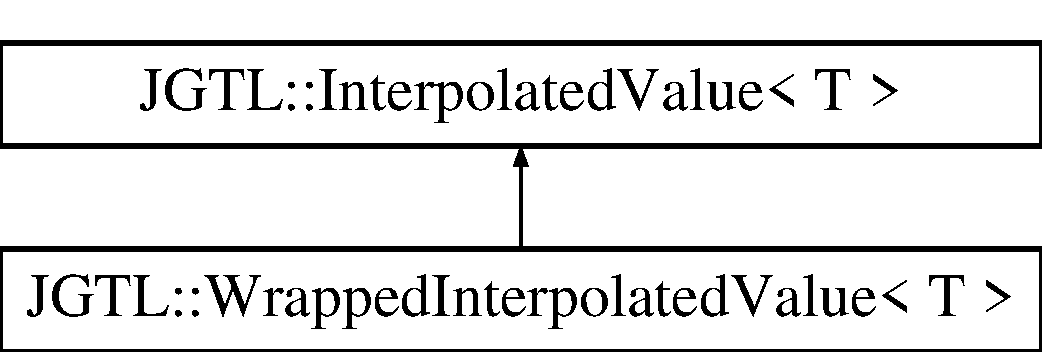
\includegraphics[height=2cm]{class_j_g_t_l_1_1_wrapped_interpolated_value}
\end{center}
\end{figure}
\subsection*{Public Member Functions}
\begin{CompactItemize}
\item 
\hyperlink{class_j_g_t_l_1_1_wrapped_interpolated_value_ee757c96b36d3c8f65accff6005e5c11}{Wrapped\-Interpolated\-Value} (const T \&\_\-min\-Value, const T \&\_\-max\-Value)
\item 
\hyperlink{class_j_g_t_l_1_1_wrapped_interpolated_value_689683a55642976810f0f244f644f814}{Wrapped\-Interpolated\-Value} (float \_\-interpolation\-Coeff, const T \&\_\-min\-Value, const T \&\_\-max\-Value)
\item 
\hyperlink{class_j_g_t_l_1_1_wrapped_interpolated_value_a5c969b821b5c9b1bd4342688264c82c}{Wrapped\-Interpolated\-Value} (const T \&\_\-value, float \_\-interpolation\-Coeff, const T \&\_\-min\-Value, const T \&\_\-max\-Value)
\item 
const \hyperlink{class_j_g_t_l_1_1_wrapped_interpolated_value}{Wrapped\-Interpolated\-Value}$<$ T $>$ \& \hyperlink{class_j_g_t_l_1_1_wrapped_interpolated_value_0608de450007ab26e20cd9a680da7e84}{operator=} (T \_\-potential\-Value)
\item 
virtual void \hyperlink{class_j_g_t_l_1_1_wrapped_interpolated_value_1cc76107e67afe602b384a1ecc9e2840}{set\-Value} (const T \&\_\-value)
\item 
virtual void \hyperlink{class_j_g_t_l_1_1_wrapped_interpolated_value_2bdc736eda165b27af022bae1f352aae}{update} (int times=1)
\end{CompactItemize}
\subsection*{Protected Member Functions}
\begin{CompactItemize}
\item 
void \hyperlink{class_j_g_t_l_1_1_wrapped_interpolated_value_eb23a3589cb6fb75cdcea67e12286ea4}{clamp\-Values} ()
\end{CompactItemize}
\subsection*{Protected Attributes}
\begin{CompactItemize}
\item 
T \hyperlink{class_j_g_t_l_1_1_wrapped_interpolated_value_7d460dd7979c409f93fc0c2d65c58a93}{min\-Value}
\item 
T \hyperlink{class_j_g_t_l_1_1_wrapped_interpolated_value_9781648d382fb2c4cbb90a6385189992}{max\-Value}
\item 
T \hyperlink{class_j_g_t_l_1_1_wrapped_interpolated_value_6b4723237650b21c40b191477207c953}{spread}
\end{CompactItemize}


\subsection{Detailed Description}
\subsubsection*{template$<$class T$>$ class JGTL::Wrapped\-Interpolated\-Value$<$ T $>$}

The \hyperlink{class_j_g_t_l_1_1_wrapped_interpolated_value}{Wrapped\-Interpolated\-Value} Class handles values which approach a limit using the formula New\-Value = actual\-Value + (potential\-Value-actual\-Value)$\ast$interpolation\-Coeff; This special instance of an \hyperlink{class_j_g_t_l_1_1_interpolated_value}{Interpolated\-Value} is for values which wrap (angles, for example, which wrap around 2$\ast$PI). 

\begin{Desc}
\item[Author:]Jason Gauci \end{Desc}
\begin{Desc}
\item[Date:]2008 \end{Desc}




\subsection{Constructor \& Destructor Documentation}
\hypertarget{class_j_g_t_l_1_1_wrapped_interpolated_value_ee757c96b36d3c8f65accff6005e5c11}{
\index{JGTL::WrappedInterpolatedValue@{JGTL::Wrapped\-Interpolated\-Value}!WrappedInterpolatedValue@{WrappedInterpolatedValue}}
\index{WrappedInterpolatedValue@{WrappedInterpolatedValue}!JGTL::WrappedInterpolatedValue@{JGTL::Wrapped\-Interpolated\-Value}}
\subsubsection[WrappedInterpolatedValue]{\setlength{\rightskip}{0pt plus 5cm}template$<$class T$>$ \hyperlink{class_j_g_t_l_1_1_wrapped_interpolated_value}{JGTL::Wrapped\-Interpolated\-Value}$<$ T $>$::\hyperlink{class_j_g_t_l_1_1_wrapped_interpolated_value}{Wrapped\-Interpolated\-Value} (const T \& {\em \_\-min\-Value}, const T \& {\em \_\-max\-Value})\hspace{0.3cm}{\tt  \mbox{[}inline\mbox{]}}}}
\label{class_j_g_t_l_1_1_wrapped_interpolated_value_ee757c96b36d3c8f65accff6005e5c11}


\hypertarget{class_j_g_t_l_1_1_wrapped_interpolated_value_689683a55642976810f0f244f644f814}{
\index{JGTL::WrappedInterpolatedValue@{JGTL::Wrapped\-Interpolated\-Value}!WrappedInterpolatedValue@{WrappedInterpolatedValue}}
\index{WrappedInterpolatedValue@{WrappedInterpolatedValue}!JGTL::WrappedInterpolatedValue@{JGTL::Wrapped\-Interpolated\-Value}}
\subsubsection[WrappedInterpolatedValue]{\setlength{\rightskip}{0pt plus 5cm}template$<$class T$>$ \hyperlink{class_j_g_t_l_1_1_wrapped_interpolated_value}{JGTL::Wrapped\-Interpolated\-Value}$<$ T $>$::\hyperlink{class_j_g_t_l_1_1_wrapped_interpolated_value}{Wrapped\-Interpolated\-Value} (float {\em \_\-interpolation\-Coeff}, const T \& {\em \_\-min\-Value}, const T \& {\em \_\-max\-Value})\hspace{0.3cm}{\tt  \mbox{[}inline\mbox{]}}}}
\label{class_j_g_t_l_1_1_wrapped_interpolated_value_689683a55642976810f0f244f644f814}


\hypertarget{class_j_g_t_l_1_1_wrapped_interpolated_value_a5c969b821b5c9b1bd4342688264c82c}{
\index{JGTL::WrappedInterpolatedValue@{JGTL::Wrapped\-Interpolated\-Value}!WrappedInterpolatedValue@{WrappedInterpolatedValue}}
\index{WrappedInterpolatedValue@{WrappedInterpolatedValue}!JGTL::WrappedInterpolatedValue@{JGTL::Wrapped\-Interpolated\-Value}}
\subsubsection[WrappedInterpolatedValue]{\setlength{\rightskip}{0pt plus 5cm}template$<$class T$>$ \hyperlink{class_j_g_t_l_1_1_wrapped_interpolated_value}{JGTL::Wrapped\-Interpolated\-Value}$<$ T $>$::\hyperlink{class_j_g_t_l_1_1_wrapped_interpolated_value}{Wrapped\-Interpolated\-Value} (const T \& {\em \_\-value}, float {\em \_\-interpolation\-Coeff}, const T \& {\em \_\-min\-Value}, const T \& {\em \_\-max\-Value})\hspace{0.3cm}{\tt  \mbox{[}inline\mbox{]}}}}
\label{class_j_g_t_l_1_1_wrapped_interpolated_value_a5c969b821b5c9b1bd4342688264c82c}




\subsection{Member Function Documentation}
\hypertarget{class_j_g_t_l_1_1_wrapped_interpolated_value_0608de450007ab26e20cd9a680da7e84}{
\index{JGTL::WrappedInterpolatedValue@{JGTL::Wrapped\-Interpolated\-Value}!operator=@{operator=}}
\index{operator=@{operator=}!JGTL::WrappedInterpolatedValue@{JGTL::Wrapped\-Interpolated\-Value}}
\subsubsection[operator=]{\setlength{\rightskip}{0pt plus 5cm}template$<$class T$>$ const \hyperlink{class_j_g_t_l_1_1_wrapped_interpolated_value}{Wrapped\-Interpolated\-Value}$<$T$>$\& \hyperlink{class_j_g_t_l_1_1_wrapped_interpolated_value}{JGTL::Wrapped\-Interpolated\-Value}$<$ T $>$::operator= (T {\em \_\-potential\-Value})\hspace{0.3cm}{\tt  \mbox{[}inline\mbox{]}}}}
\label{class_j_g_t_l_1_1_wrapped_interpolated_value_0608de450007ab26e20cd9a680da7e84}




Reimplemented from \hyperlink{class_j_g_t_l_1_1_interpolated_value_30b679bad94ef7adf003bf99e5756a53}{JGTL::Interpolated\-Value$<$ T $>$}.\hypertarget{class_j_g_t_l_1_1_wrapped_interpolated_value_1cc76107e67afe602b384a1ecc9e2840}{
\index{JGTL::WrappedInterpolatedValue@{JGTL::Wrapped\-Interpolated\-Value}!setValue@{setValue}}
\index{setValue@{setValue}!JGTL::WrappedInterpolatedValue@{JGTL::Wrapped\-Interpolated\-Value}}
\subsubsection[setValue]{\setlength{\rightskip}{0pt plus 5cm}template$<$class T$>$ virtual void \hyperlink{class_j_g_t_l_1_1_wrapped_interpolated_value}{JGTL::Wrapped\-Interpolated\-Value}$<$ T $>$::set\-Value (const T \& {\em \_\-value})\hspace{0.3cm}{\tt  \mbox{[}inline, virtual\mbox{]}}}}
\label{class_j_g_t_l_1_1_wrapped_interpolated_value_1cc76107e67afe602b384a1ecc9e2840}




Reimplemented from \hyperlink{class_j_g_t_l_1_1_interpolated_value_eaeff236b97efbf0c616333e1b94b210}{JGTL::Interpolated\-Value$<$ T $>$}.\hypertarget{class_j_g_t_l_1_1_wrapped_interpolated_value_2bdc736eda165b27af022bae1f352aae}{
\index{JGTL::WrappedInterpolatedValue@{JGTL::Wrapped\-Interpolated\-Value}!update@{update}}
\index{update@{update}!JGTL::WrappedInterpolatedValue@{JGTL::Wrapped\-Interpolated\-Value}}
\subsubsection[update]{\setlength{\rightskip}{0pt plus 5cm}template$<$class T$>$ virtual void \hyperlink{class_j_g_t_l_1_1_wrapped_interpolated_value}{JGTL::Wrapped\-Interpolated\-Value}$<$ T $>$::update (int {\em times} = {\tt 1})\hspace{0.3cm}{\tt  \mbox{[}inline, virtual\mbox{]}}}}
\label{class_j_g_t_l_1_1_wrapped_interpolated_value_2bdc736eda165b27af022bae1f352aae}




Reimplemented from \hyperlink{class_j_g_t_l_1_1_interpolated_value_bc1a6a8d484921bc309289c400bf0fbe}{JGTL::Interpolated\-Value$<$ T $>$}.\hypertarget{class_j_g_t_l_1_1_wrapped_interpolated_value_eb23a3589cb6fb75cdcea67e12286ea4}{
\index{JGTL::WrappedInterpolatedValue@{JGTL::Wrapped\-Interpolated\-Value}!clampValues@{clampValues}}
\index{clampValues@{clampValues}!JGTL::WrappedInterpolatedValue@{JGTL::Wrapped\-Interpolated\-Value}}
\subsubsection[clampValues]{\setlength{\rightskip}{0pt plus 5cm}template$<$class T$>$ void \hyperlink{class_j_g_t_l_1_1_wrapped_interpolated_value}{JGTL::Wrapped\-Interpolated\-Value}$<$ T $>$::clamp\-Values ()\hspace{0.3cm}{\tt  \mbox{[}inline, protected\mbox{]}}}}
\label{class_j_g_t_l_1_1_wrapped_interpolated_value_eb23a3589cb6fb75cdcea67e12286ea4}




\subsection{Member Data Documentation}
\hypertarget{class_j_g_t_l_1_1_wrapped_interpolated_value_7d460dd7979c409f93fc0c2d65c58a93}{
\index{JGTL::WrappedInterpolatedValue@{JGTL::Wrapped\-Interpolated\-Value}!minValue@{minValue}}
\index{minValue@{minValue}!JGTL::WrappedInterpolatedValue@{JGTL::Wrapped\-Interpolated\-Value}}
\subsubsection[minValue]{\setlength{\rightskip}{0pt plus 5cm}template$<$class T$>$ T \hyperlink{class_j_g_t_l_1_1_wrapped_interpolated_value}{JGTL::Wrapped\-Interpolated\-Value}$<$ T $>$::\hyperlink{class_j_g_t_l_1_1_wrapped_interpolated_value_7d460dd7979c409f93fc0c2d65c58a93}{min\-Value}\hspace{0.3cm}{\tt  \mbox{[}protected\mbox{]}}}}
\label{class_j_g_t_l_1_1_wrapped_interpolated_value_7d460dd7979c409f93fc0c2d65c58a93}


\hypertarget{class_j_g_t_l_1_1_wrapped_interpolated_value_9781648d382fb2c4cbb90a6385189992}{
\index{JGTL::WrappedInterpolatedValue@{JGTL::Wrapped\-Interpolated\-Value}!maxValue@{maxValue}}
\index{maxValue@{maxValue}!JGTL::WrappedInterpolatedValue@{JGTL::Wrapped\-Interpolated\-Value}}
\subsubsection[maxValue]{\setlength{\rightskip}{0pt plus 5cm}template$<$class T$>$ T \hyperlink{class_j_g_t_l_1_1_wrapped_interpolated_value}{JGTL::Wrapped\-Interpolated\-Value}$<$ T $>$::\hyperlink{class_j_g_t_l_1_1_wrapped_interpolated_value_9781648d382fb2c4cbb90a6385189992}{max\-Value}\hspace{0.3cm}{\tt  \mbox{[}protected\mbox{]}}}}
\label{class_j_g_t_l_1_1_wrapped_interpolated_value_9781648d382fb2c4cbb90a6385189992}


\hypertarget{class_j_g_t_l_1_1_wrapped_interpolated_value_6b4723237650b21c40b191477207c953}{
\index{JGTL::WrappedInterpolatedValue@{JGTL::Wrapped\-Interpolated\-Value}!spread@{spread}}
\index{spread@{spread}!JGTL::WrappedInterpolatedValue@{JGTL::Wrapped\-Interpolated\-Value}}
\subsubsection[spread]{\setlength{\rightskip}{0pt plus 5cm}template$<$class T$>$ T \hyperlink{class_j_g_t_l_1_1_wrapped_interpolated_value}{JGTL::Wrapped\-Interpolated\-Value}$<$ T $>$::\hyperlink{class_j_g_t_l_1_1_wrapped_interpolated_value_6b4723237650b21c40b191477207c953}{spread}\hspace{0.3cm}{\tt  \mbox{[}protected\mbox{]}}}}
\label{class_j_g_t_l_1_1_wrapped_interpolated_value_6b4723237650b21c40b191477207c953}




The documentation for this class was generated from the following file:\begin{CompactItemize}
\item 
\hyperlink{_j_g_t_l___wrapped_interpolated_value_8h}{JGTL\_\-Wrapped\-Interpolated\-Value.h}\end{CompactItemize}

\hypertarget{class_j_g_t_l_1_1_xor_space}{
\section{JGTL::Xor\-Space$<$ Rectangle, Point $>$ Class Template Reference}
\label{class_j_g_t_l_1_1_xor_space}\index{JGTL::XorSpace@{JGTL::XorSpace}}
}
This class handles Xor spaces. Think of this as a way to handle things like rectangular doughnuts. A positive space followed by a smaller concentric negative space would represent a doughnut.  


{\tt \#include $<$JGTL\_\-Xor\-Space.h$>$}

\subsection*{Public Types}
\begin{CompactItemize}
\item 
typedef vector$<$ \hyperlink{class_j_g_t_l_1_1_xor_space_rect}{Xor\-Space\-Rect}$<$ Rectangle, Point $>$ $>$::iterator \hyperlink{class_j_g_t_l_1_1_xor_space_17c93bf8f2f8ec86efcc3e4a63e4a6ef}{Space\-Iterator}
\item 
typedef vector$<$ \hyperlink{class_j_g_t_l_1_1_xor_space_rect}{Xor\-Space\-Rect}$<$ Rectangle, Point $>$ $>$::const\_\-iterator \hyperlink{class_j_g_t_l_1_1_xor_space_467518dcd95f1c3f009f59ad3ea5d8df}{Const\-Space\-Iterator}
\end{CompactItemize}
\subsection*{Public Member Functions}
\begin{CompactItemize}
\item 
\hyperlink{class_j_g_t_l_1_1_xor_space_ad236c36d98b3fbf0d592ea1a524c34d}{Xor\-Space} ()
\item 
\hyperlink{class_j_g_t_l_1_1_xor_space_7ba86691f975e9e55e71ff94e46b7855}{Xor\-Space} (const Rectangle \&start)
\item 
void \hyperlink{class_j_g_t_l_1_1_xor_space_0f5b4faaaf03b9c7f85302125e2e834b}{add\-Space} (const Rectangle \&space, bool positive)
\item 
void \hyperlink{class_j_g_t_l_1_1_xor_space_ade3a68cc488df5f40a33df407887c2f}{remove\-Space} (const Rectangle \&space, bool positive)
\item 
bool \hyperlink{class_j_g_t_l_1_1_xor_space_327d98abef98ac5263a081a96cdc12ec}{contains} (const Point \&point) const 
\item 
const Point \& \hyperlink{class_j_g_t_l_1_1_xor_space_cb61e4508a4df0ab8dc83db8ce75140a}{get\-Top\-Left} () const
\item 
const Point \& \hyperlink{class_j_g_t_l_1_1_xor_space_20f62e7360534b0d7f9945acc99627d1}{get\-Bottom\-Right} () const
\item 
Point \hyperlink{class_j_g_t_l_1_1_xor_space_497ef0f83c9d2b6cdc10c4b297fd6e4f}{get\-Size} () const
\item 
Point \hyperlink{class_j_g_t_l_1_1_xor_space_fc844c1202940bc5340cf01a4431cbab}{get\-First\-Point} () const
\item 
bool \hyperlink{class_j_g_t_l_1_1_xor_space_88d290e087366c43f48ba39f3df78931}{get\-Next\-Point} (Point \&cur\-Point) const 
\item 
void \hyperlink{class_j_g_t_l_1_1_xor_space_a699867cb9debc04136fbbc8ccc4ff6f}{pack} ()
\end{CompactItemize}
\subsection*{Protected Attributes}
\begin{CompactItemize}
\item 
vector$<$ \hyperlink{class_j_g_t_l_1_1_xor_space_rect}{Xor\-Space\-Rect}$<$ Rectangle, Point $>$ $>$ \hyperlink{class_j_g_t_l_1_1_xor_space_107013005de6d1b3b7c5e6067b2054c5}{spaces}
\item 
Point \hyperlink{class_j_g_t_l_1_1_xor_space_9220f06140cf547c2521372da2d97f80}{top\-Left}
\item 
Point \hyperlink{class_j_g_t_l_1_1_xor_space_e76eebb329d0056211ff1c0caee42364}{bottom\-Right}
\end{CompactItemize}


\subsection{Detailed Description}
\subsubsection*{template$<$class Rectangle, class Point$>$ class JGTL::Xor\-Space$<$ Rectangle, Point $>$}

This class handles Xor spaces. Think of this as a way to handle things like rectangular doughnuts. A positive space followed by a smaller concentric negative space would represent a doughnut. 

\begin{Desc}
\item[Author:]Jason Gauci \end{Desc}
\begin{Desc}
\item[Date:]2008 \end{Desc}




\subsection{Member Typedef Documentation}
\hypertarget{class_j_g_t_l_1_1_xor_space_17c93bf8f2f8ec86efcc3e4a63e4a6ef}{
\index{JGTL::XorSpace@{JGTL::Xor\-Space}!SpaceIterator@{SpaceIterator}}
\index{SpaceIterator@{SpaceIterator}!JGTL::XorSpace@{JGTL::Xor\-Space}}
\subsubsection[SpaceIterator]{\setlength{\rightskip}{0pt plus 5cm}template$<$class Rectangle, class Point$>$ typedef vector$<$ \hyperlink{class_j_g_t_l_1_1_xor_space_rect}{Xor\-Space\-Rect}$<$Rectangle,Point$>$ $>$::iterator \hyperlink{class_j_g_t_l_1_1_xor_space}{JGTL::Xor\-Space}$<$ Rectangle, Point $>$::\hyperlink{class_j_g_t_l_1_1_xor_space_17c93bf8f2f8ec86efcc3e4a63e4a6ef}{Space\-Iterator}}}
\label{class_j_g_t_l_1_1_xor_space_17c93bf8f2f8ec86efcc3e4a63e4a6ef}


\hypertarget{class_j_g_t_l_1_1_xor_space_467518dcd95f1c3f009f59ad3ea5d8df}{
\index{JGTL::XorSpace@{JGTL::Xor\-Space}!ConstSpaceIterator@{ConstSpaceIterator}}
\index{ConstSpaceIterator@{ConstSpaceIterator}!JGTL::XorSpace@{JGTL::Xor\-Space}}
\subsubsection[ConstSpaceIterator]{\setlength{\rightskip}{0pt plus 5cm}template$<$class Rectangle, class Point$>$ typedef vector$<$ \hyperlink{class_j_g_t_l_1_1_xor_space_rect}{Xor\-Space\-Rect}$<$Rectangle,Point$>$ $>$::const\_\-iterator \hyperlink{class_j_g_t_l_1_1_xor_space}{JGTL::Xor\-Space}$<$ Rectangle, Point $>$::\hyperlink{class_j_g_t_l_1_1_xor_space_467518dcd95f1c3f009f59ad3ea5d8df}{Const\-Space\-Iterator}}}
\label{class_j_g_t_l_1_1_xor_space_467518dcd95f1c3f009f59ad3ea5d8df}




\subsection{Constructor \& Destructor Documentation}
\hypertarget{class_j_g_t_l_1_1_xor_space_ad236c36d98b3fbf0d592ea1a524c34d}{
\index{JGTL::XorSpace@{JGTL::Xor\-Space}!XorSpace@{XorSpace}}
\index{XorSpace@{XorSpace}!JGTL::XorSpace@{JGTL::Xor\-Space}}
\subsubsection[XorSpace]{\setlength{\rightskip}{0pt plus 5cm}template$<$class Rectangle, class Point$>$ \hyperlink{class_j_g_t_l_1_1_xor_space}{JGTL::Xor\-Space}$<$ Rectangle, Point $>$::\hyperlink{class_j_g_t_l_1_1_xor_space}{Xor\-Space} ()\hspace{0.3cm}{\tt  \mbox{[}inline\mbox{]}}}}
\label{class_j_g_t_l_1_1_xor_space_ad236c36d98b3fbf0d592ea1a524c34d}


\hypertarget{class_j_g_t_l_1_1_xor_space_7ba86691f975e9e55e71ff94e46b7855}{
\index{JGTL::XorSpace@{JGTL::Xor\-Space}!XorSpace@{XorSpace}}
\index{XorSpace@{XorSpace}!JGTL::XorSpace@{JGTL::Xor\-Space}}
\subsubsection[XorSpace]{\setlength{\rightskip}{0pt plus 5cm}template$<$class Rectangle, class Point$>$ \hyperlink{class_j_g_t_l_1_1_xor_space}{JGTL::Xor\-Space}$<$ Rectangle, Point $>$::\hyperlink{class_j_g_t_l_1_1_xor_space}{Xor\-Space} (const Rectangle \& {\em start})\hspace{0.3cm}{\tt  \mbox{[}inline\mbox{]}}}}
\label{class_j_g_t_l_1_1_xor_space_7ba86691f975e9e55e71ff94e46b7855}




\subsection{Member Function Documentation}
\hypertarget{class_j_g_t_l_1_1_xor_space_0f5b4faaaf03b9c7f85302125e2e834b}{
\index{JGTL::XorSpace@{JGTL::Xor\-Space}!addSpace@{addSpace}}
\index{addSpace@{addSpace}!JGTL::XorSpace@{JGTL::Xor\-Space}}
\subsubsection[addSpace]{\setlength{\rightskip}{0pt plus 5cm}template$<$class Rectangle, class Point$>$ void \hyperlink{class_j_g_t_l_1_1_xor_space}{JGTL::Xor\-Space}$<$ Rectangle, Point $>$::add\-Space (const Rectangle \& {\em space}, bool {\em positive})\hspace{0.3cm}{\tt  \mbox{[}inline\mbox{]}}}}
\label{class_j_g_t_l_1_1_xor_space_0f5b4faaaf03b9c7f85302125e2e834b}


Adds a space with the highest priority to the list of spaces. \begin{Desc}
\item[Parameters:]
\begin{description}
\item[{\em space}]The rectangle to add \item[{\em positive}]Whether the rectangle is positive or negative (a negative cancels all positives before it) \end{description}
\end{Desc}
\hypertarget{class_j_g_t_l_1_1_xor_space_ade3a68cc488df5f40a33df407887c2f}{
\index{JGTL::XorSpace@{JGTL::Xor\-Space}!removeSpace@{removeSpace}}
\index{removeSpace@{removeSpace}!JGTL::XorSpace@{JGTL::Xor\-Space}}
\subsubsection[removeSpace]{\setlength{\rightskip}{0pt plus 5cm}template$<$class Rectangle, class Point$>$ void \hyperlink{class_j_g_t_l_1_1_xor_space}{JGTL::Xor\-Space}$<$ Rectangle, Point $>$::remove\-Space (const Rectangle \& {\em space}, bool {\em positive})\hspace{0.3cm}{\tt  \mbox{[}inline\mbox{]}}}}
\label{class_j_g_t_l_1_1_xor_space_ade3a68cc488df5f40a33df407887c2f}


Removes a space with the lowest priority and a certain size and polarity \begin{Desc}
\item[Parameters:]
\begin{description}
\item[{\em space}]The rectangle to add \item[{\em positive}]Whether the rectangle is positive or negative (a negative cancels all positives before it) \end{description}
\end{Desc}
\hypertarget{class_j_g_t_l_1_1_xor_space_327d98abef98ac5263a081a96cdc12ec}{
\index{JGTL::XorSpace@{JGTL::Xor\-Space}!contains@{contains}}
\index{contains@{contains}!JGTL::XorSpace@{JGTL::Xor\-Space}}
\subsubsection[contains]{\setlength{\rightskip}{0pt plus 5cm}template$<$class Rectangle, class Point$>$ bool \hyperlink{class_j_g_t_l_1_1_xor_space}{JGTL::Xor\-Space}$<$ Rectangle, Point $>$::contains (const Point \& {\em point}) const\hspace{0.3cm}{\tt  \mbox{[}inline\mbox{]}}}}
\label{class_j_g_t_l_1_1_xor_space_327d98abef98ac5263a081a96cdc12ec}


Checks if the \hyperlink{class_j_g_t_l_1_1_xor_space}{Xor\-Space} contains a certain point \hypertarget{class_j_g_t_l_1_1_xor_space_cb61e4508a4df0ab8dc83db8ce75140a}{
\index{JGTL::XorSpace@{JGTL::Xor\-Space}!getTopLeft@{getTopLeft}}
\index{getTopLeft@{getTopLeft}!JGTL::XorSpace@{JGTL::Xor\-Space}}
\subsubsection[getTopLeft]{\setlength{\rightskip}{0pt plus 5cm}template$<$class Rectangle, class Point$>$ const Point\& \hyperlink{class_j_g_t_l_1_1_xor_space}{JGTL::Xor\-Space}$<$ Rectangle, Point $>$::get\-Top\-Left () const\hspace{0.3cm}{\tt  \mbox{[}inline\mbox{]}}}}
\label{class_j_g_t_l_1_1_xor_space_cb61e4508a4df0ab8dc83db8ce75140a}


\hypertarget{class_j_g_t_l_1_1_xor_space_20f62e7360534b0d7f9945acc99627d1}{
\index{JGTL::XorSpace@{JGTL::Xor\-Space}!getBottomRight@{getBottomRight}}
\index{getBottomRight@{getBottomRight}!JGTL::XorSpace@{JGTL::Xor\-Space}}
\subsubsection[getBottomRight]{\setlength{\rightskip}{0pt plus 5cm}template$<$class Rectangle, class Point$>$ const Point\& \hyperlink{class_j_g_t_l_1_1_xor_space}{JGTL::Xor\-Space}$<$ Rectangle, Point $>$::get\-Bottom\-Right () const\hspace{0.3cm}{\tt  \mbox{[}inline\mbox{]}}}}
\label{class_j_g_t_l_1_1_xor_space_20f62e7360534b0d7f9945acc99627d1}


\hypertarget{class_j_g_t_l_1_1_xor_space_497ef0f83c9d2b6cdc10c4b297fd6e4f}{
\index{JGTL::XorSpace@{JGTL::Xor\-Space}!getSize@{getSize}}
\index{getSize@{getSize}!JGTL::XorSpace@{JGTL::Xor\-Space}}
\subsubsection[getSize]{\setlength{\rightskip}{0pt plus 5cm}template$<$class Rectangle, class Point$>$ Point \hyperlink{class_j_g_t_l_1_1_xor_space}{JGTL::Xor\-Space}$<$ Rectangle, Point $>$::get\-Size () const\hspace{0.3cm}{\tt  \mbox{[}inline\mbox{]}}}}
\label{class_j_g_t_l_1_1_xor_space_497ef0f83c9d2b6cdc10c4b297fd6e4f}


\hypertarget{class_j_g_t_l_1_1_xor_space_fc844c1202940bc5340cf01a4431cbab}{
\index{JGTL::XorSpace@{JGTL::Xor\-Space}!getFirstPoint@{getFirstPoint}}
\index{getFirstPoint@{getFirstPoint}!JGTL::XorSpace@{JGTL::Xor\-Space}}
\subsubsection[getFirstPoint]{\setlength{\rightskip}{0pt plus 5cm}template$<$class Rectangle, class Point$>$ Point \hyperlink{class_j_g_t_l_1_1_xor_space}{JGTL::Xor\-Space}$<$ Rectangle, Point $>$::get\-First\-Point () const\hspace{0.3cm}{\tt  \mbox{[}inline\mbox{]}}}}
\label{class_j_g_t_l_1_1_xor_space_fc844c1202940bc5340cf01a4431cbab}


Returns the top-left point of an Xor-Space \hypertarget{class_j_g_t_l_1_1_xor_space_88d290e087366c43f48ba39f3df78931}{
\index{JGTL::XorSpace@{JGTL::Xor\-Space}!getNextPoint@{getNextPoint}}
\index{getNextPoint@{getNextPoint}!JGTL::XorSpace@{JGTL::Xor\-Space}}
\subsubsection[getNextPoint]{\setlength{\rightskip}{0pt plus 5cm}template$<$class Rectangle, class Point$>$ bool \hyperlink{class_j_g_t_l_1_1_xor_space}{JGTL::Xor\-Space}$<$ Rectangle, Point $>$::get\-Next\-Point (Point \& {\em cur\-Point}) const\hspace{0.3cm}{\tt  \mbox{[}inline\mbox{]}}}}
\label{class_j_g_t_l_1_1_xor_space_88d290e087366c43f48ba39f3df78931}


Gets the next point within an \hyperlink{class_j_g_t_l_1_1_xor_space}{Xor\-Space}. Works along with \hyperlink{class_j_g_t_l_1_1_xor_space_fc844c1202940bc5340cf01a4431cbab}{get\-First\-Point()} to iterate over all points. \hypertarget{class_j_g_t_l_1_1_xor_space_a699867cb9debc04136fbbc8ccc4ff6f}{
\index{JGTL::XorSpace@{JGTL::Xor\-Space}!pack@{pack}}
\index{pack@{pack}!JGTL::XorSpace@{JGTL::Xor\-Space}}
\subsubsection[pack]{\setlength{\rightskip}{0pt plus 5cm}template$<$class Rectangle, class Point$>$ void \hyperlink{class_j_g_t_l_1_1_xor_space}{JGTL::Xor\-Space}$<$ Rectangle, Point $>$::pack ()\hspace{0.3cm}{\tt  \mbox{[}inline\mbox{]}}}}
\label{class_j_g_t_l_1_1_xor_space_a699867cb9debc04136fbbc8ccc4ff6f}


Tries to eliminate redundant spaces in an \hyperlink{class_j_g_t_l_1_1_xor_space}{Xor\-Space} 

\subsection{Member Data Documentation}
\hypertarget{class_j_g_t_l_1_1_xor_space_107013005de6d1b3b7c5e6067b2054c5}{
\index{JGTL::XorSpace@{JGTL::Xor\-Space}!spaces@{spaces}}
\index{spaces@{spaces}!JGTL::XorSpace@{JGTL::Xor\-Space}}
\subsubsection[spaces]{\setlength{\rightskip}{0pt plus 5cm}template$<$class Rectangle, class Point$>$ vector$<$\hyperlink{class_j_g_t_l_1_1_xor_space_rect}{Xor\-Space\-Rect}$<$Rectangle,Point$>$ $>$ \hyperlink{class_j_g_t_l_1_1_xor_space}{JGTL::Xor\-Space}$<$ Rectangle, Point $>$::\hyperlink{class_j_g_t_l_1_1_xor_space_107013005de6d1b3b7c5e6067b2054c5}{spaces}\hspace{0.3cm}{\tt  \mbox{[}protected\mbox{]}}}}
\label{class_j_g_t_l_1_1_xor_space_107013005de6d1b3b7c5e6067b2054c5}


\hypertarget{class_j_g_t_l_1_1_xor_space_9220f06140cf547c2521372da2d97f80}{
\index{JGTL::XorSpace@{JGTL::Xor\-Space}!topLeft@{topLeft}}
\index{topLeft@{topLeft}!JGTL::XorSpace@{JGTL::Xor\-Space}}
\subsubsection[topLeft]{\setlength{\rightskip}{0pt plus 5cm}template$<$class Rectangle, class Point$>$ Point \hyperlink{class_j_g_t_l_1_1_xor_space}{JGTL::Xor\-Space}$<$ Rectangle, Point $>$::\hyperlink{class_j_g_t_l_1_1_xor_space_9220f06140cf547c2521372da2d97f80}{top\-Left}\hspace{0.3cm}{\tt  \mbox{[}protected\mbox{]}}}}
\label{class_j_g_t_l_1_1_xor_space_9220f06140cf547c2521372da2d97f80}


\hypertarget{class_j_g_t_l_1_1_xor_space_e76eebb329d0056211ff1c0caee42364}{
\index{JGTL::XorSpace@{JGTL::Xor\-Space}!bottomRight@{bottomRight}}
\index{bottomRight@{bottomRight}!JGTL::XorSpace@{JGTL::Xor\-Space}}
\subsubsection[bottomRight]{\setlength{\rightskip}{0pt plus 5cm}template$<$class Rectangle, class Point$>$ Point \hyperlink{class_j_g_t_l_1_1_xor_space}{JGTL::Xor\-Space}$<$ Rectangle, Point $>$::\hyperlink{class_j_g_t_l_1_1_xor_space_e76eebb329d0056211ff1c0caee42364}{bottom\-Right}\hspace{0.3cm}{\tt  \mbox{[}protected\mbox{]}}}}
\label{class_j_g_t_l_1_1_xor_space_e76eebb329d0056211ff1c0caee42364}




The documentation for this class was generated from the following file:\begin{CompactItemize}
\item 
\hyperlink{_j_g_t_l___xor_space_8h}{JGTL\_\-Xor\-Space.h}\end{CompactItemize}

\hypertarget{class_j_g_t_l_1_1_xor_space_rect}{
\section{JGTL::Xor\-Space\-Rect$<$ Rectangle, Point $>$ Class Template Reference}
\label{class_j_g_t_l_1_1_xor_space_rect}\index{JGTL::XorSpaceRect@{JGTL::XorSpaceRect}}
}
This handles a single Xor Rectangle.  


{\tt \#include $<$JGTL\_\-Xor\-Space.h$>$}

\subsection*{Public Member Functions}
\begin{CompactItemize}
\item 
\hyperlink{class_j_g_t_l_1_1_xor_space_rect_aeeac5078979658fb7234c36c7faab90}{Xor\-Space\-Rect} ()
\item 
\hyperlink{class_j_g_t_l_1_1_xor_space_rect_7e23ca980e665ef6bea0e1f8052a2628}{Xor\-Space\-Rect} (Rectangle \_\-rect, bool \_\-positive)
\end{CompactItemize}
\subsection*{Public Attributes}
\begin{CompactItemize}
\item 
Rectangle \hyperlink{class_j_g_t_l_1_1_xor_space_rect_5cb60d58273133694cc1f0c821471603}{rect}
\item 
bool \hyperlink{class_j_g_t_l_1_1_xor_space_rect_20faa85ce2e1856b7a94a7613f7a6074}{positive}
\end{CompactItemize}


\subsection{Detailed Description}
\subsubsection*{template$<$class Rectangle, class Point$>$ class JGTL::Xor\-Space\-Rect$<$ Rectangle, Point $>$}

This handles a single Xor Rectangle. 

\begin{Desc}
\item[Author:]Jason Gauci \end{Desc}
\begin{Desc}
\item[Date:]2008 \end{Desc}




\subsection{Constructor \& Destructor Documentation}
\hypertarget{class_j_g_t_l_1_1_xor_space_rect_aeeac5078979658fb7234c36c7faab90}{
\index{JGTL::XorSpaceRect@{JGTL::Xor\-Space\-Rect}!XorSpaceRect@{XorSpaceRect}}
\index{XorSpaceRect@{XorSpaceRect}!JGTL::XorSpaceRect@{JGTL::Xor\-Space\-Rect}}
\subsubsection[XorSpaceRect]{\setlength{\rightskip}{0pt plus 5cm}template$<$class Rectangle, class Point$>$ \hyperlink{class_j_g_t_l_1_1_xor_space_rect}{JGTL::Xor\-Space\-Rect}$<$ Rectangle, Point $>$::\hyperlink{class_j_g_t_l_1_1_xor_space_rect}{Xor\-Space\-Rect} ()\hspace{0.3cm}{\tt  \mbox{[}inline\mbox{]}}}}
\label{class_j_g_t_l_1_1_xor_space_rect_aeeac5078979658fb7234c36c7faab90}


\hypertarget{class_j_g_t_l_1_1_xor_space_rect_7e23ca980e665ef6bea0e1f8052a2628}{
\index{JGTL::XorSpaceRect@{JGTL::Xor\-Space\-Rect}!XorSpaceRect@{XorSpaceRect}}
\index{XorSpaceRect@{XorSpaceRect}!JGTL::XorSpaceRect@{JGTL::Xor\-Space\-Rect}}
\subsubsection[XorSpaceRect]{\setlength{\rightskip}{0pt plus 5cm}template$<$class Rectangle, class Point$>$ \hyperlink{class_j_g_t_l_1_1_xor_space_rect}{JGTL::Xor\-Space\-Rect}$<$ Rectangle, Point $>$::\hyperlink{class_j_g_t_l_1_1_xor_space_rect}{Xor\-Space\-Rect} (Rectangle {\em \_\-rect}, bool {\em \_\-positive})\hspace{0.3cm}{\tt  \mbox{[}inline\mbox{]}}}}
\label{class_j_g_t_l_1_1_xor_space_rect_7e23ca980e665ef6bea0e1f8052a2628}




\subsection{Member Data Documentation}
\hypertarget{class_j_g_t_l_1_1_xor_space_rect_5cb60d58273133694cc1f0c821471603}{
\index{JGTL::XorSpaceRect@{JGTL::Xor\-Space\-Rect}!rect@{rect}}
\index{rect@{rect}!JGTL::XorSpaceRect@{JGTL::Xor\-Space\-Rect}}
\subsubsection[rect]{\setlength{\rightskip}{0pt plus 5cm}template$<$class Rectangle, class Point$>$ Rectangle \hyperlink{class_j_g_t_l_1_1_xor_space_rect}{JGTL::Xor\-Space\-Rect}$<$ Rectangle, Point $>$::\hyperlink{class_j_g_t_l_1_1_xor_space_rect_5cb60d58273133694cc1f0c821471603}{rect}}}
\label{class_j_g_t_l_1_1_xor_space_rect_5cb60d58273133694cc1f0c821471603}


\hypertarget{class_j_g_t_l_1_1_xor_space_rect_20faa85ce2e1856b7a94a7613f7a6074}{
\index{JGTL::XorSpaceRect@{JGTL::Xor\-Space\-Rect}!positive@{positive}}
\index{positive@{positive}!JGTL::XorSpaceRect@{JGTL::Xor\-Space\-Rect}}
\subsubsection[positive]{\setlength{\rightskip}{0pt plus 5cm}template$<$class Rectangle, class Point$>$ bool \hyperlink{class_j_g_t_l_1_1_xor_space_rect}{JGTL::Xor\-Space\-Rect}$<$ Rectangle, Point $>$::\hyperlink{class_j_g_t_l_1_1_xor_space_rect_20faa85ce2e1856b7a94a7613f7a6074}{positive}}}
\label{class_j_g_t_l_1_1_xor_space_rect_20faa85ce2e1856b7a94a7613f7a6074}




The documentation for this class was generated from the following file:\begin{CompactItemize}
\item 
\hyperlink{_j_g_t_l___xor_space_8h}{JGTL\_\-Xor\-Space.h}\end{CompactItemize}

\chapter{JGTL File Documentation}
\hypertarget{_j_g_t_l___bar_8h}{
\section{JGTL\_\-Bar.h File Reference}
\label{_j_g_t_l___bar_8h}\index{JGTL_Bar.h@{JGTL\_\-Bar.h}}
}
\subsection*{Namespaces}
\begin{CompactItemize}
\item 
namespace \hyperlink{namespace_j_g_t_l}{JGTL}
\end{CompactItemize}
\subsection*{Classes}
\begin{CompactItemize}
\item 
class \hyperlink{class_j_g_t_l_1_1_bar}{JGTL::Bar$<$ Bar\-Value\-Type $>$}
\begin{CompactList}\small\item\em The \hyperlink{class_j_g_t_l_1_1_bar}{Bar} Class handles a max/current value system (e.g. a Progress \hyperlink{class_j_g_t_l_1_1_bar}{Bar}). \item\end{CompactList}\end{CompactItemize}
\subsection*{Functions}
\begin{CompactItemize}
\item 
template$<$class Bar\-Value\-Type$>$ ostream \& \hyperlink{namespace_j_g_t_l_c7b88574d9cbabb871f978d45333686d}{JGTL::operator$<$$<$} (ostream \&stream, const Bar$<$ Bar\-Value\-Type $>$ \&d)
\item 
template$<$class Bar\-Value\-Type$>$ istream \& \hyperlink{namespace_j_g_t_l_092a0993d280d2d4dbb45d96e9d40abc}{JGTL::operator$>$$>$} (istream \&stream, Bar$<$ Bar\-Value\-Type $>$ \&d)
\end{CompactItemize}

\hypertarget{_j_g_t_l___circular_buffer_8h}{
\section{JGTL\_\-Circular\-Buffer.h File Reference}
\label{_j_g_t_l___circular_buffer_8h}\index{JGTL_CircularBuffer.h@{JGTL\_\-CircularBuffer.h}}
}
{\tt \#include $<$utility$>$}\par
{\tt \#include $<$cstdlib$>$}\par
{\tt \#include \char`\"{}JGTL\_\-Located\-Exception.h\char`\"{}}\par
\subsection*{Namespaces}
\begin{CompactItemize}
\item 
namespace \hyperlink{namespace_j_g_t_l}{JGTL}
\end{CompactItemize}
\subsection*{Classes}
\begin{CompactItemize}
\item 
class \hyperlink{class_j_g_t_l_1_1_circular_buffer}{JGTL::Circular\-Buffer$<$ Data $>$}
\begin{CompactList}\small\item\em The \hyperlink{class_j_g_t_l_1_1_circular_buffer}{Circular\-Buffer} Class handles a Circular Buffer. \item\end{CompactList}\end{CompactItemize}
\subsection*{Defines}
\begin{CompactItemize}
\item 
\#define \hyperlink{_j_g_t_l___circular_buffer_8h_7afb109397da024c7fd554ca83ec284d}{DEBUG\_\-CIRCULAR\_\-BUFFER}~(0)
\end{CompactItemize}


\subsection{Define Documentation}
\hypertarget{_j_g_t_l___circular_buffer_8h_7afb109397da024c7fd554ca83ec284d}{
\index{JGTL_CircularBuffer.h@{JGTL\_\-Circular\-Buffer.h}!DEBUG_CIRCULAR_BUFFER@{DEBUG\_\-CIRCULAR\_\-BUFFER}}
\index{DEBUG_CIRCULAR_BUFFER@{DEBUG\_\-CIRCULAR\_\-BUFFER}!JGTL_CircularBuffer.h@{JGTL\_\-Circular\-Buffer.h}}
\subsubsection[DEBUG\_\-CIRCULAR\_\-BUFFER]{\setlength{\rightskip}{0pt plus 5cm}\#define DEBUG\_\-CIRCULAR\_\-BUFFER~(0)}}
\label{_j_g_t_l___circular_buffer_8h_7afb109397da024c7fd554ca83ec284d}



\hypertarget{_j_g_t_l___circular_buffer_interface_8h}{
\section{JGTL\_\-Circular\-Buffer\-Interface.h File Reference}
\label{_j_g_t_l___circular_buffer_interface_8h}\index{JGTL_CircularBufferInterface.h@{JGTL\_\-CircularBufferInterface.h}}
}
{\tt \#include $<$utility$>$}\par
{\tt \#include $<$cstdlib$>$}\par
{\tt \#include \char`\"{}JGTL\_\-Located\-Exception.h\char`\"{}}\par
\subsection*{Namespaces}
\begin{CompactItemize}
\item 
namespace \hyperlink{namespace_j_g_t_l}{JGTL}
\end{CompactItemize}
\subsection*{Classes}
\begin{CompactItemize}
\item 
class \hyperlink{class_j_g_t_l_1_1_circular_buffer_interface}{JGTL::Circular\-Buffer\-Interface$<$ Data $>$}
\begin{CompactList}\small\item\em The \hyperlink{class_j_g_t_l_1_1_circular_buffer_interface}{Circular\-Buffer\-Interface} Class handles a Circular Buffer. \item\end{CompactList}\end{CompactItemize}
\subsection*{Defines}
\begin{CompactItemize}
\item 
\#define \hyperlink{_j_g_t_l___circular_buffer_interface_8h_aec9cd10e36869f7a348abd67b240548}{DEBUG\_\-CIRCULAR\_\-BUFFER\_\-INTERFACE}~(0)
\end{CompactItemize}


\subsection{Define Documentation}
\hypertarget{_j_g_t_l___circular_buffer_interface_8h_aec9cd10e36869f7a348abd67b240548}{
\index{JGTL_CircularBufferInterface.h@{JGTL\_\-Circular\-Buffer\-Interface.h}!DEBUG_CIRCULAR_BUFFER_INTERFACE@{DEBUG\_\-CIRCULAR\_\-BUFFER\_\-INTERFACE}}
\index{DEBUG_CIRCULAR_BUFFER_INTERFACE@{DEBUG\_\-CIRCULAR\_\-BUFFER\_\-INTERFACE}!JGTL_CircularBufferInterface.h@{JGTL\_\-Circular\-Buffer\-Interface.h}}
\subsubsection[DEBUG\_\-CIRCULAR\_\-BUFFER\_\-INTERFACE]{\setlength{\rightskip}{0pt plus 5cm}\#define DEBUG\_\-CIRCULAR\_\-BUFFER\_\-INTERFACE~(0)}}
\label{_j_g_t_l___circular_buffer_interface_8h_aec9cd10e36869f7a348abd67b240548}



\hypertarget{_j_g_t_l___command_line_parser_8h}{
\section{JGTL\_\-Command\-Line\-Parser.h File Reference}
\label{_j_g_t_l___command_line_parser_8h}\index{JGTL_CommandLineParser.h@{JGTL\_\-CommandLineParser.h}}
}
{\tt \#include $<$map$>$}\par
{\tt \#include $<$string$>$}\par
{\tt \#include $<$vector$>$}\par
\subsection*{Namespaces}
\begin{CompactItemize}
\item 
namespace \hyperlink{namespace_j_g_t_l}{JGTL}
\end{CompactItemize}
\subsection*{Classes}
\begin{CompactItemize}
\item 
struct \hyperlink{struct_j_g_t_l_1_1_c_cmd_param}{JGTL::CCmd\-Param}
\item 
class \hyperlink{class_j_g_t_l_1_1_command_line_parser}{JGTL::Command\-Line\-Parser}
\end{CompactItemize}
\subsection*{Defines}
\begin{CompactItemize}
\item 
\#define \hyperlink{_j_g_t_l___command_line_parser_8h_4f4ee4d9513ba224014f4ef6759b2241}{String\-Type}~std::string
\end{CompactItemize}
\subsection*{Typedefs}
\begin{CompactItemize}
\item 
typedef std::map$<$ String\-Type, CCmd\-Param $>$ \hyperlink{namespace_j_g_t_l_93797b96f684075b65783b93d11f2f1d}{JGTL::\_\-Command\-Line\-Parser}
\end{CompactItemize}


\subsection{Define Documentation}
\hypertarget{_j_g_t_l___command_line_parser_8h_4f4ee4d9513ba224014f4ef6759b2241}{
\index{JGTL_CommandLineParser.h@{JGTL\_\-Command\-Line\-Parser.h}!StringType@{StringType}}
\index{StringType@{StringType}!JGTL_CommandLineParser.h@{JGTL\_\-Command\-Line\-Parser.h}}
\subsubsection[StringType]{\setlength{\rightskip}{0pt plus 5cm}\#define String\-Type~std::string}}
\label{_j_g_t_l___command_line_parser_8h_4f4ee4d9513ba224014f4ef6759b2241}



\hypertarget{_j_g_t_l___data_manager_8h}{
\section{JGTL\_\-Data\-Manager.h File Reference}
\label{_j_g_t_l___data_manager_8h}\index{JGTL_DataManager.h@{JGTL\_\-DataManager.h}}
}
{\tt \#include $<$cstdlib$>$}\par
{\tt \#include $<$cctype$>$}\par
{\tt \#include $<$string$>$}\par
{\tt \#include $<$algorithm$>$}\par
{\tt \#include \char`\"{}JGTL\_\-Located\-Exception.h\char`\"{}}\par
\subsection*{Namespaces}
\begin{CompactItemize}
\item 
namespace \hyperlink{namespace_j_g_t_l}{JGTL}
\end{CompactItemize}
\subsection*{Classes}
\begin{CompactItemize}
\item 
class \hyperlink{class_j_g_t_l_1_1_data_manager}{JGTL::Data\-Manager$<$ Data $>$}
\end{CompactItemize}
\subsection*{Defines}
\begin{CompactItemize}
\item 
\#define \hyperlink{_j_g_t_l___data_manager_8h_d2df8db18baa2d2fb1d0722d12a1d407}{DEBUG\_\-DATA\_\-MANAGER}~(0)
\end{CompactItemize}


\subsection{Define Documentation}
\hypertarget{_j_g_t_l___data_manager_8h_d2df8db18baa2d2fb1d0722d12a1d407}{
\index{JGTL_DataManager.h@{JGTL\_\-Data\-Manager.h}!DEBUG_DATA_MANAGER@{DEBUG\_\-DATA\_\-MANAGER}}
\index{DEBUG_DATA_MANAGER@{DEBUG\_\-DATA\_\-MANAGER}!JGTL_DataManager.h@{JGTL\_\-Data\-Manager.h}}
\subsubsection[DEBUG\_\-DATA\_\-MANAGER]{\setlength{\rightskip}{0pt plus 5cm}\#define DEBUG\_\-DATA\_\-MANAGER~(0)}}
\label{_j_g_t_l___data_manager_8h_d2df8db18baa2d2fb1d0722d12a1d407}



\hypertarget{_j_g_t_l___data_pool__delete_8h}{
\section{JGTL\_\-Data\-Pool\_\-delete.h File Reference}
\label{_j_g_t_l___data_pool__delete_8h}\index{JGTL_DataPool_delete.h@{JGTL\_\-DataPool\_\-delete.h}}
}
{\tt \#include $<$memory$>$}\par
{\tt \#include \char`\"{}JGTL\_\-Located\-Exception.h\char`\"{}}\par
\subsection*{Namespaces}
\begin{CompactItemize}
\item 
namespace \hyperlink{namespace_j_g_t_l}{JGTL}
\end{CompactItemize}
\subsection*{Classes}
\begin{CompactItemize}
\item 
class \hyperlink{class_j_g_t_l_1_1_data_pool}{JGTL::Data\-Pool$<$ Data $>$}
\end{CompactItemize}
\subsection*{Defines}
\begin{CompactItemize}
\item 
\#define \hyperlink{_j_g_t_l___data_pool__delete_8h_d42e79f451587676a0744f59d0bdc965}{DEBUG\_\-DATA\_\-POOL}~(0)
\end{CompactItemize}


\subsection{Define Documentation}
\hypertarget{_j_g_t_l___data_pool__delete_8h_d42e79f451587676a0744f59d0bdc965}{
\index{JGTL_DataPool_delete.h@{JGTL\_\-Data\-Pool\_\-delete.h}!DEBUG_DATA_POOL@{DEBUG\_\-DATA\_\-POOL}}
\index{DEBUG_DATA_POOL@{DEBUG\_\-DATA\_\-POOL}!JGTL_DataPool_delete.h@{JGTL\_\-Data\-Pool\_\-delete.h}}
\subsubsection[DEBUG\_\-DATA\_\-POOL]{\setlength{\rightskip}{0pt plus 5cm}\#define DEBUG\_\-DATA\_\-POOL~(0)}}
\label{_j_g_t_l___data_pool__delete_8h_d42e79f451587676a0744f59d0bdc965}



\hypertarget{_j_g_t_l___dynamic_circular_buffer_8h}{
\section{JGTL\_\-Dynamic\-Circular\-Buffer.h File Reference}
\label{_j_g_t_l___dynamic_circular_buffer_8h}\index{JGTL_DynamicCircularBuffer.h@{JGTL\_\-DynamicCircularBuffer.h}}
}
{\tt \#include $<$utility$>$}\par
{\tt \#include $<$cstdlib$>$}\par
{\tt \#include \char`\"{}JGTL\_\-Located\-Exception.h\char`\"{}}\par
{\tt \#include \char`\"{}JGTL\_\-Circular\-Buffer\-Interface.h\char`\"{}}\par
\subsection*{Namespaces}
\begin{CompactItemize}
\item 
namespace \hyperlink{namespace_j_g_t_l}{JGTL}
\end{CompactItemize}
\subsection*{Classes}
\begin{CompactItemize}
\item 
class \hyperlink{class_j_g_t_l_1_1_dynamic_circular_buffer}{JGTL::Dynamic\-Circular\-Buffer$<$ Data $>$}
\begin{CompactList}\small\item\em The \hyperlink{class_j_g_t_l_1_1_dynamic_circular_buffer}{Dynamic\-Circular\-Buffer} Class handles a Circular Buffer. \item\end{CompactList}\end{CompactItemize}
\subsection*{Defines}
\begin{CompactItemize}
\item 
\#define \hyperlink{_j_g_t_l___dynamic_circular_buffer_8h_0e1b293a18ffbba6ef6a6dabeda10555}{DEBUG\_\-DYNAMIC\_\-CIRCULAR\_\-BUFFER}~(0)
\end{CompactItemize}


\subsection{Define Documentation}
\hypertarget{_j_g_t_l___dynamic_circular_buffer_8h_0e1b293a18ffbba6ef6a6dabeda10555}{
\index{JGTL_DynamicCircularBuffer.h@{JGTL\_\-Dynamic\-Circular\-Buffer.h}!DEBUG_DYNAMIC_CIRCULAR_BUFFER@{DEBUG\_\-DYNAMIC\_\-CIRCULAR\_\-BUFFER}}
\index{DEBUG_DYNAMIC_CIRCULAR_BUFFER@{DEBUG\_\-DYNAMIC\_\-CIRCULAR\_\-BUFFER}!JGTL_DynamicCircularBuffer.h@{JGTL\_\-Dynamic\-Circular\-Buffer.h}}
\subsubsection[DEBUG\_\-DYNAMIC\_\-CIRCULAR\_\-BUFFER]{\setlength{\rightskip}{0pt plus 5cm}\#define DEBUG\_\-DYNAMIC\_\-CIRCULAR\_\-BUFFER~(0)}}
\label{_j_g_t_l___dynamic_circular_buffer_8h_0e1b293a18ffbba6ef6a6dabeda10555}



\include{_j_g_t_l___dynamic_pool_map_8h}
\hypertarget{_j_g_t_l___dynamic_pool_set_8h}{
\section{JGTL\_\-Dynamic\-Pool\-Set.h File Reference}
\label{_j_g_t_l___dynamic_pool_set_8h}\index{JGTL_DynamicPoolSet.h@{JGTL\_\-DynamicPoolSet.h}}
}
{\tt \#include $<$utility$>$}\par
{\tt \#include $<$cstdlib$>$}\par
{\tt \#include \char`\"{}JGTL\_\-Located\-Exception.h\char`\"{}}\par
{\tt \#include \char`\"{}JGTL\_\-Set\-Interface.h\char`\"{}}\par
\subsection*{Namespaces}
\begin{CompactItemize}
\item 
namespace \hyperlink{namespace_j_g_t_l}{JGTL}
\end{CompactItemize}
\subsection*{Classes}
\begin{CompactItemize}
\item 
class \hyperlink{class_j_g_t_l_1_1_dynamic_pool_set}{JGTL::Dynamic\-Pool\-Set$<$ Data $>$}
\end{CompactItemize}
\subsection*{Defines}
\begin{CompactItemize}
\item 
\#define \hyperlink{_j_g_t_l___dynamic_pool_set_8h_6734c3d136e33b5ff6721e66d6adaf43}{DEBUG\_\-DYNAMIC\_\-POOL\_\-SET}~(0)
\end{CompactItemize}


\subsection{Define Documentation}
\hypertarget{_j_g_t_l___dynamic_pool_set_8h_6734c3d136e33b5ff6721e66d6adaf43}{
\index{JGTL_DynamicPoolSet.h@{JGTL\_\-Dynamic\-Pool\-Set.h}!DEBUG_DYNAMIC_POOL_SET@{DEBUG\_\-DYNAMIC\_\-POOL\_\-SET}}
\index{DEBUG_DYNAMIC_POOL_SET@{DEBUG\_\-DYNAMIC\_\-POOL\_\-SET}!JGTL_DynamicPoolSet.h@{JGTL\_\-Dynamic\-Pool\-Set.h}}
\subsubsection[DEBUG\_\-DYNAMIC\_\-POOL\_\-SET]{\setlength{\rightskip}{0pt plus 5cm}\#define DEBUG\_\-DYNAMIC\_\-POOL\_\-SET~(0)}}
\label{_j_g_t_l___dynamic_pool_set_8h_6734c3d136e33b5ff6721e66d6adaf43}



\hypertarget{_j_g_t_l___floating_units_8h}{
\section{JGTL\_\-Floating\-Units.h File Reference}
\label{_j_g_t_l___floating_units_8h}\index{JGTL_FloatingUnits.h@{JGTL\_\-FloatingUnits.h}}
}
{\tt \#include $<$iostream$>$}\par
{\tt \#include $<$complex$>$}\par
{\tt \#include $<$sstream$>$}\par
\subsection*{Namespaces}
\begin{CompactItemize}
\item 
namespace \hyperlink{namespace_j_g_t_l}{JGTL}
\end{CompactItemize}
\subsection*{Classes}
\begin{CompactItemize}
\item 
class \hyperlink{class_j_g_t_l_1_1_floating_units}{JGTL::Floating\-Units$<$ Value\-Type, SCALE\_\-NUMERATOR, SCALE\_\-DENOMINATOR $>$}
\end{CompactItemize}
\subsection*{Typedefs}
\begin{CompactItemize}
\item 
typedef unsigned long long \hyperlink{namespace_j_g_t_l_1924d6fd42e2d9661bc0b5a5063b99b3}{JGTL::units\_\-internal\_\-ulong}
\end{CompactItemize}
\subsection*{Functions}
\begin{CompactItemize}
\item 
template$<$class Value\-Type, units\_\-internal\_\-ulong SCALE\_\-NUMERATOR, units\_\-internal\_\-ulong SCALE\_\-DENOMINATOR$>$ std::ostream \& \hyperlink{namespace_j_g_t_l_86ab99d9902f6c5772fb0adc0cb2a020}{JGTL::operator$<$$<$} (std::ostream \&stream, const Floating\-Units$<$ Value\-Type, SCALE\_\-NUMERATOR, SCALE\_\-DENOMINATOR $>$ \&d)
\item 
template$<$class Value\-Type, units\_\-internal\_\-ulong SCALE\_\-NUMERATOR, units\_\-internal\_\-ulong SCALE\_\-DENOMINATOR$>$ std::istream \& \hyperlink{namespace_j_g_t_l_6c3aa6e2c845fd00bac1728506725fa8}{JGTL::operator$>$$>$} (std::istream \&stream, Floating\-Units$<$ Value\-Type, SCALE\_\-NUMERATOR, SCALE\_\-DENOMINATOR $>$ \&d)
\end{CompactItemize}

\hypertarget{_j_g_t_l___hex_tree_8h}{
\section{JGTL\_\-Hex\-Tree.h File Reference}
\label{_j_g_t_l___hex_tree_8h}\index{JGTL_HexTree.h@{JGTL\_\-HexTree.h}}
}
{\tt \#include $<$iostream$>$}\par
{\tt \#include $<$string$>$}\par
{\tt \#include \char`\"{}Vector4.h\char`\"{}}\par
{\tt \#include \char`\"{}boost/pool/pool.hpp\char`\"{}}\par
\subsection*{Namespaces}
\begin{CompactItemize}
\item 
namespace \hyperlink{namespace_j_g_t_l}{JGTL}
\item 
namespace \hyperlink{namespacestd}{std}
\end{CompactItemize}
\subsection*{Classes}
\begin{CompactItemize}
\item 
class \hyperlink{class_j_g_t_l_1_1_hex_tree_node}{JGTL::Hex\-Tree\-Node$<$ T $>$}
\item 
class \hyperlink{class_j_g_t_l_1_1_hex_tree_stub}{JGTL::Hex\-Tree\-Stub$<$ T $>$}
\item 
class \hyperlink{class_j_g_t_l_1_1_hex_tree_branch}{JGTL::Hex\-Tree\-Branch$<$ T $>$}
\item 
class \hyperlink{class_j_g_t_l_1_1_hex_tree}{JGTL::Hex\-Tree$<$ T $>$}
\end{CompactItemize}

\hypertarget{_j_g_t_l___index2_8h}{
\section{JGTL\_\-Index2.h File Reference}
\label{_j_g_t_l___index2_8h}\index{JGTL_Index2.h@{JGTL\_\-Index2.h}}
}
\subsection*{Namespaces}
\begin{CompactItemize}
\item 
namespace \hyperlink{namespace_j_g_t_l}{JGTL}
\end{CompactItemize}
\subsection*{Classes}
\begin{CompactItemize}
\item 
class \hyperlink{class_j_g_t_l_1_1_index2}{JGTL::Index2}
\end{CompactItemize}

\hypertarget{_j_g_t_l___index3_8h}{
\section{JGTL\_\-Index3.h File Reference}
\label{_j_g_t_l___index3_8h}\index{JGTL_Index3.h@{JGTL\_\-Index3.h}}
}
{\tt \#include $<$algorithm$>$}\par
{\tt \#include $<$iostream$>$}\par
{\tt \#include $<$cmath$>$}\par
\subsection*{Namespaces}
\begin{CompactItemize}
\item 
namespace \hyperlink{namespace_j_g_t_l}{JGTL}
\end{CompactItemize}
\subsection*{Classes}
\begin{CompactItemize}
\item 
class \hyperlink{class_j_g_t_l_1_1_index3}{JGTL::Index3}
\item 
class \hyperlink{class_j_g_t_l_1_1_rectangle_index3}{JGTL::Rectangle\-Index3}
\end{CompactItemize}
\subsection*{Functions}
\begin{CompactItemize}
\item 
ostream \& \hyperlink{namespace_j_g_t_l_da86017e720d1a0d7bc6ee620e6e798f}{JGTL::operator$<$$<$} (ostream \&stream, const Index3 \&d)
\item 
istream \& \hyperlink{namespace_j_g_t_l_2b5020a887bfbfcf78f56c3181a47ace}{JGTL::operator$>$$>$} (istream \&stream, Index3 \&d)
\end{CompactItemize}

\hypertarget{_j_g_t_l___integral_units_8h}{
\section{JGTL\_\-Integral\-Units.h File Reference}
\label{_j_g_t_l___integral_units_8h}\index{JGTL_IntegralUnits.h@{JGTL\_\-IntegralUnits.h}}
}
{\tt \#include $<$iostream$>$}\par
{\tt \#include $<$complex$>$}\par
{\tt \#include $<$sstream$>$}\par
\subsection*{Namespaces}
\begin{CompactItemize}
\item 
namespace \hyperlink{namespace_j_g_t_l}{JGTL}
\end{CompactItemize}
\subsection*{Classes}
\begin{CompactItemize}
\item 
struct \hyperlink{struct_j_g_t_l_1_1_i_f}{JGTL::IF$<$ condition, Then, Else $>$}
\item 
struct \hyperlink{struct_j_g_t_l_1_1_i_f_3_01false_00_01_then_00_01_else_01_4}{JGTL::IF$<$ false, Then, Else $>$}
\item 
struct \hyperlink{struct_j_g_t_l_1_1_s_t_a_t_i_c___m_o_d}{JGTL::STATIC\_\-MOD$<$ Type, a, b $>$}
\item 
struct \hyperlink{struct_j_g_t_l_1_1_t_y_p_e_i_f}{JGTL::TYPEIF$<$ Type, condition, Then, Else $>$}
\item 
struct \hyperlink{struct_j_g_t_l_1_1_t_y_p_e_i_f_3_01_type_00_01false_00_01_then_00_01_else_01_4}{JGTL::TYPEIF$<$ Type, false, Then, Else $>$}
\item 
struct \hyperlink{struct_j_g_t_l_1_1_integral_units_g_c_d}{JGTL::Integral\-Units\-GCD$<$ i, j $>$}
\item 
struct \hyperlink{struct_j_g_t_l_1_1_integral_units_g_c_d_3_011_00_01j_01_4}{JGTL::Integral\-Units\-GCD$<$ 1, j $>$}
\item 
struct \hyperlink{struct_j_g_t_l_1_1_integral_units_g_c_d_3_01i_00_011_01_4}{JGTL::Integral\-Units\-GCD$<$ i, 1 $>$}
\item 
struct \hyperlink{struct_j_g_t_l_1_1_integral_units_g_c_d_3_011_00_011_01_4}{JGTL::Integral\-Units\-GCD$<$ 1, 1 $>$}
\item 
struct \hyperlink{struct_j_g_t_l_1_1_integral_units_g_c_d_3_010_00_01j_01_4}{JGTL::Integral\-Units\-GCD$<$ 0, j $>$}
\item 
struct \hyperlink{struct_j_g_t_l_1_1_integral_units_g_c_d_3_01i_00_010_01_4}{JGTL::Integral\-Units\-GCD$<$ i, 0 $>$}
\item 
struct \hyperlink{struct_j_g_t_l_1_1_integral_units_g_c_d_3_010_00_010_01_4}{JGTL::Integral\-Units\-GCD$<$ 0, 0 $>$}
\item 
class \hyperlink{class_j_g_t_l_1_1_integral_units}{JGTL::Integral\-Units$<$ Value\-Type, SCALE, USEGCD $>$}
\end{CompactItemize}
\subsection*{Typedefs}
\begin{CompactItemize}
\item 
typedef unsigned long long \hyperlink{namespace_j_g_t_l_1924d6fd42e2d9661bc0b5a5063b99b3}{JGTL::units\_\-internal\_\-ulong}
\end{CompactItemize}
\subsection*{Functions}
\begin{CompactItemize}
\item 
template$<$class T$>$ units\_\-internal\_\-ulong \hyperlink{namespace_j_g_t_l_5d540b652d4a0d15e83ae5daa5695edd}{JGTL::GCD} (T a, T b)
\item 
template$<$$>$ units\_\-internal\_\-ulong \hyperlink{namespace_j_g_t_l_3288a482038d7cc9db66241879178908}{JGTL::GCD} (double a, double b)
\item 
template$<$$>$ units\_\-internal\_\-ulong \hyperlink{namespace_j_g_t_l_25c40254ef74d292898efc841fa19182}{JGTL::GCD} (float a, float b)
\item 
template$<$class Value\-Type, Value\-Type SCALE, bool USEGCD$>$ std::ostream \& \hyperlink{namespace_j_g_t_l_bb4eaae6cdeb0bb91835f543745cf38e}{JGTL::operator$<$$<$} (std::ostream \&stream, const Integral\-Units$<$ Value\-Type, SCALE, USEGCD $>$ \&d)
\item 
template$<$class Value\-Type, Value\-Type SCALE, bool USEGCD$>$ std::istream \& \hyperlink{namespace_j_g_t_l_e2329341531898d1534dbc7ecb0b6a21}{JGTL::operator$>$$>$} (std::istream \&stream, Integral\-Units$<$ Value\-Type, SCALE, USEGCD $>$ \&d)
\end{CompactItemize}

\hypertarget{_j_g_t_l___interpolated_value_8h}{
\section{JGTL\_\-Interpolated\-Value.h File Reference}
\label{_j_g_t_l___interpolated_value_8h}\index{JGTL_InterpolatedValue.h@{JGTL\_\-InterpolatedValue.h}}
}
\subsection*{Namespaces}
\begin{CompactItemize}
\item 
namespace \hyperlink{namespace_j_g_t_l}{JGTL}
\end{CompactItemize}
\subsection*{Classes}
\begin{CompactItemize}
\item 
class \hyperlink{class_j_g_t_l_1_1_interpolated_value}{JGTL::Interpolated\-Value$<$ T $>$}
\begin{CompactList}\small\item\em The \hyperlink{class_j_g_t_l_1_1_interpolated_value}{Interpolated\-Value} Class handles values which approach a limit using the formula New\-Value = actual\-Value + (potential\-Value-actual\-Value)$\ast$interpolation\-Coeff;. \item\end{CompactList}\end{CompactItemize}
\subsection*{Functions}
\begin{CompactItemize}
\item 
template$<$class T$>$ std::ostream \& \hyperlink{namespace_j_g_t_l_14895317a64983a968bb8236dd6e32d5}{JGTL::operator$<$$<$} (std::ostream \&stream, const Interpolated\-Value$<$ T $>$ \&d)
\item 
template$<$class T$>$ std::istream \& \hyperlink{namespace_j_g_t_l_40f708595d5793876f680b255589f642}{JGTL::operator$>$$>$} (std::istream \&stream, Interpolated\-Value$<$ T $>$ \&d)
\end{CompactItemize}

\hypertarget{_j_g_t_l___located_exception_8h}{
\section{JGTL\_\-Located\-Exception.h File Reference}
\label{_j_g_t_l___located_exception_8h}\index{JGTL_LocatedException.h@{JGTL\_\-LocatedException.h}}
}
{\tt \#include $<$string$>$}\par
{\tt \#include $<$sstream$>$}\par
\subsection*{Namespaces}
\begin{CompactItemize}
\item 
namespace \hyperlink{namespace_j_g_t_l}{JGTL}
\end{CompactItemize}
\subsection*{Classes}
\begin{CompactItemize}
\item 
class \hyperlink{class_j_g_t_l_1_1_located_exception}{JGTL::Located\-Exception}
\begin{CompactList}\small\item\em This class handles throwing exceptions which include the file and line number. \item\end{CompactList}\end{CompactItemize}
\subsection*{Defines}
\begin{CompactItemize}
\item 
\#define \hyperlink{_j_g_t_l___located_exception_8h_fb222c40cffcdc9db02e5fb9b0e3a204}{CREATE\_\-PAUSE}(X)~\{cout $<$$<$ X $<$$<$ \char`\"{}$\backslash$n\-Press enter to continue\char`\"{} $<$$<$ endl;string line;getline(cin,line);\}
\item 
\#define \hyperlink{_j_g_t_l___located_exception_8h_4bda3acfa8613f0bee44fc645143e9d3}{CREATE\_\-LOCATEDEXCEPTION\_\-INFO}(X)~\hyperlink{class_j_g_t_l_1_1_located_exception}{JGTL::Located\-Exception}( (X) ,\_\-\_\-FILE\_\-\_\-,\_\-\_\-LINE\_\-\_\-);
\end{CompactItemize}


\subsection{Define Documentation}
\hypertarget{_j_g_t_l___located_exception_8h_4bda3acfa8613f0bee44fc645143e9d3}{
\index{JGTL_LocatedException.h@{JGTL\_\-Located\-Exception.h}!CREATE_LOCATEDEXCEPTION_INFO@{CREATE\_\-LOCATEDEXCEPTION\_\-INFO}}
\index{CREATE_LOCATEDEXCEPTION_INFO@{CREATE\_\-LOCATEDEXCEPTION\_\-INFO}!JGTL_LocatedException.h@{JGTL\_\-Located\-Exception.h}}
\subsubsection[CREATE\_\-LOCATEDEXCEPTION\_\-INFO]{\setlength{\rightskip}{0pt plus 5cm}\#define CREATE\_\-LOCATEDEXCEPTION\_\-INFO(X)~\hyperlink{class_j_g_t_l_1_1_located_exception}{JGTL::Located\-Exception}( (X) ,\_\-\_\-FILE\_\-\_\-,\_\-\_\-LINE\_\-\_\-);}}
\label{_j_g_t_l___located_exception_8h_4bda3acfa8613f0bee44fc645143e9d3}


\hypertarget{_j_g_t_l___located_exception_8h_fb222c40cffcdc9db02e5fb9b0e3a204}{
\index{JGTL_LocatedException.h@{JGTL\_\-Located\-Exception.h}!CREATE_PAUSE@{CREATE\_\-PAUSE}}
\index{CREATE_PAUSE@{CREATE\_\-PAUSE}!JGTL_LocatedException.h@{JGTL\_\-Located\-Exception.h}}
\subsubsection[CREATE\_\-PAUSE]{\setlength{\rightskip}{0pt plus 5cm}\#define CREATE\_\-PAUSE(X)~\{cout $<$$<$ X $<$$<$ \char`\"{}$\backslash$n\-Press enter to continue\char`\"{} $<$$<$ endl;string line;getline(cin,line);\}}}
\label{_j_g_t_l___located_exception_8h_fb222c40cffcdc9db02e5fb9b0e3a204}



\hypertarget{_j_g_t_l___map_interface_8h}{
\section{JGTL\_\-Map\-Interface.h File Reference}
\label{_j_g_t_l___map_interface_8h}\index{JGTL_MapInterface.h@{JGTL\_\-MapInterface.h}}
}
{\tt \#include $<$utility$>$}\par
{\tt \#include $<$cstdlib$>$}\par
{\tt \#include \char`\"{}JGTL\_\-Located\-Exception.h\char`\"{}}\par
\subsection*{Namespaces}
\begin{CompactItemize}
\item 
namespace \hyperlink{namespace_j_g_t_l}{JGTL}
\end{CompactItemize}
\subsection*{Classes}
\begin{CompactItemize}
\item 
class \hyperlink{class_j_g_t_l_1_1_map_interface}{JGTL::Map\-Interface$<$ Key, Data $>$}
\begin{CompactList}\small\item\em This class acts as a base class for the Map construct. \item\end{CompactList}\end{CompactItemize}
\subsection*{Defines}
\begin{CompactItemize}
\item 
\#define \hyperlink{_j_g_t_l___map_interface_8h_df99d6b59685be518d4e47848e9fbfee}{DEBUG\_\-MAP\_\-INTERFACE}~(0)
\end{CompactItemize}


\subsection{Define Documentation}
\hypertarget{_j_g_t_l___map_interface_8h_df99d6b59685be518d4e47848e9fbfee}{
\index{JGTL_MapInterface.h@{JGTL\_\-Map\-Interface.h}!DEBUG_MAP_INTERFACE@{DEBUG\_\-MAP\_\-INTERFACE}}
\index{DEBUG_MAP_INTERFACE@{DEBUG\_\-MAP\_\-INTERFACE}!JGTL_MapInterface.h@{JGTL\_\-Map\-Interface.h}}
\subsubsection[DEBUG\_\-MAP\_\-INTERFACE]{\setlength{\rightskip}{0pt plus 5cm}\#define DEBUG\_\-MAP\_\-INTERFACE~(0)}}
\label{_j_g_t_l___map_interface_8h_df99d6b59685be518d4e47848e9fbfee}



\hypertarget{_j_g_t_l___poly_variant_8h}{
\section{JGTL\_\-Poly\-Variant.h File Reference}
\label{_j_g_t_l___poly_variant_8h}\index{JGTL_PolyVariant.h@{JGTL\_\-PolyVariant.h}}
}
{\tt \#include $<$iostream$>$}\par
{\tt \#include \char`\"{}JGTL\_\-Located\-Exception.h\char`\"{}}\par
{\tt \#include \char`\"{}JGTL\_\-Variant.h\char`\"{}}\par
\subsection*{Namespaces}
\begin{CompactItemize}
\item 
namespace \hyperlink{namespace_j_g_t_l}{JGTL}
\end{CompactItemize}
\subsection*{Classes}
\begin{CompactItemize}
\item 
class \hyperlink{class_j_g_t_l_1_1_poly_variant}{JGTL::Poly\-Variant$<$ Base\-Class, Class1, Class2, Class3, Class4, Class5, Class6, Class7, Class8, Class9, Class10 $>$}
\end{CompactItemize}

\hypertarget{_j_g_t_l___pool_map__delete_8h}{
\section{JGTL\_\-Pool\-Map\_\-delete.h File Reference}
\label{_j_g_t_l___pool_map__delete_8h}\index{JGTL_PoolMap_delete.h@{JGTL\_\-PoolMap\_\-delete.h}}
}
{\tt \#include $<$utility$>$}\par
{\tt \#include $<$cstdlib$>$}\par
{\tt \#include \char`\"{}JGTL\_\-Located\-Exception.h\char`\"{}}\par
\subsection*{Namespaces}
\begin{CompactItemize}
\item 
namespace \hyperlink{namespace_j_g_t_l}{JGTL}
\end{CompactItemize}
\subsection*{Classes}
\begin{CompactItemize}
\item 
class \hyperlink{class_j_g_t_l_1_1_pool_map}{JGTL::Pool\-Map$<$ Key, Data $>$}
\end{CompactItemize}
\subsection*{Defines}
\begin{CompactItemize}
\item 
\#define \hyperlink{_j_g_t_l___pool_map__delete_8h_c938b73a6d655e02f79a5baee99876b6}{DEBUG\_\-POOL\_\-MAP}~(0)
\end{CompactItemize}


\subsection{Define Documentation}
\hypertarget{_j_g_t_l___pool_map__delete_8h_c938b73a6d655e02f79a5baee99876b6}{
\index{JGTL_PoolMap_delete.h@{JGTL\_\-Pool\-Map\_\-delete.h}!DEBUG_POOL_MAP@{DEBUG\_\-POOL\_\-MAP}}
\index{DEBUG_POOL_MAP@{DEBUG\_\-POOL\_\-MAP}!JGTL_PoolMap_delete.h@{JGTL\_\-Pool\-Map\_\-delete.h}}
\subsubsection[DEBUG\_\-POOL\_\-MAP]{\setlength{\rightskip}{0pt plus 5cm}\#define DEBUG\_\-POOL\_\-MAP~(0)}}
\label{_j_g_t_l___pool_map__delete_8h_c938b73a6d655e02f79a5baee99876b6}



\hypertarget{_j_g_t_l___quad_tree_8h}{
\section{JGTL\_\-Quad\-Tree.h File Reference}
\label{_j_g_t_l___quad_tree_8h}\index{JGTL_QuadTree.h@{JGTL\_\-QuadTree.h}}
}
{\tt \#include $<$iostream$>$}\par
{\tt \#include $<$string$>$}\par
{\tt \#include \char`\"{}JGTL\_\-Vector2.h\char`\"{}}\par
{\tt \#include \char`\"{}boost/pool/pool.hpp\char`\"{}}\par
\subsection*{Namespaces}
\begin{CompactItemize}
\item 
namespace \hyperlink{namespace_j_g_t_l}{JGTL}
\end{CompactItemize}
\subsection*{Classes}
\begin{CompactItemize}
\item 
class \hyperlink{class_j_g_t_l_1_1_quad_tree_node}{JGTL::Quad\-Tree\-Node$<$ T $>$}
\item 
class \hyperlink{class_j_g_t_l_1_1_quad_tree_stub}{JGTL::Quad\-Tree\-Stub$<$ T $>$}
\item 
class \hyperlink{class_j_g_t_l_1_1_quad_tree_branch}{JGTL::Quad\-Tree\-Branch$<$ T $>$}
\item 
class \hyperlink{class_j_g_t_l_1_1_quad_tree}{JGTL::Quad\-Tree$<$ T $>$}
\end{CompactItemize}

\hypertarget{_j_g_t_l___quick_prof_8h}{
\section{JGTL\_\-Quick\-Prof.h File Reference}
\label{_j_g_t_l___quick_prof_8h}\index{JGTL_QuickProf.h@{JGTL\_\-QuickProf.h}}
}
{\tt \#include $<$iostream$>$}\par
{\tt \#include $<$fstream$>$}\par
{\tt \#include $<$sstream$>$}\par
{\tt \#include $<$math.h$>$}\par
{\tt \#include $<$algorithm$>$}\par
{\tt \#include \char`\"{}JGTL\_\-Located\-Exception.h\char`\"{}}\par
{\tt \#include \char`\"{}JGTL\_\-Dynamic\-Pool\-Map.h\char`\"{}}\par
{\tt \#include \char`\"{}JGTL\_\-Singleton.h\char`\"{}}\par
{\tt \#include $<$sys/time.h$>$}\par
\subsection*{Namespaces}
\begin{CompactItemize}
\item 
namespace \hyperlink{namespace_j_g_t_l}{JGTL}
\end{CompactItemize}
\subsection*{Classes}
\begin{CompactItemize}
\item 
struct \hyperlink{struct_j_g_t_l_1_1_profile_block}{JGTL::Profile\-Block}
\item 
class \hyperlink{class_j_g_t_l_1_1_clock}{JGTL::Clock}
\item 
class \hyperlink{class_j_g_t_l_1_1_profiler}{JGTL::Profiler}
\begin{CompactList}\small\item\em A singleton class that manages timing for a set of profiling blocks. \item\end{CompactList}\item 
class \hyperlink{class_j_g_t_l_1_1_profile_block_handler}{JGTL::Profile\-Block\-Handler}
\end{CompactItemize}
\subsection*{Defines}
\begin{CompactItemize}
\item 
\#define \hyperlink{_j_g_t_l___quick_prof_8h_19c6455991847f755a6eae9042db8f27}{PROFILER}~JGTL::Profiler::get\-Instance()
\end{CompactItemize}
\subsection*{Enumerations}
\begin{CompactItemize}
\item 
enum \hyperlink{namespace_j_g_t_l_11a34d88ecadd1c99354adc21fd5abe6}{JGTL::Time\-Format} \{ \hyperlink{namespace_j_g_t_l_11a34d88ecadd1c99354adc21fd5abe6ad29f96ec6ca22f686db310d3e491ccd}{JGTL::SECONDS}, 
\hyperlink{namespace_j_g_t_l_11a34d88ecadd1c99354adc21fd5abe60634056587e1e00ecaa18019a990c055}{JGTL::MILLISECONDS}, 
\hyperlink{namespace_j_g_t_l_11a34d88ecadd1c99354adc21fd5abe68e2289b823ea3baf8aa44b51676d3b08}{JGTL::MICROSECONDS}, 
\hyperlink{namespace_j_g_t_l_11a34d88ecadd1c99354adc21fd5abe6a5f6364e2e978c03f8500a982568cad7}{JGTL::PERCENT}
 \}
\begin{CompactList}\small\item\em A set of ways to represent timing results. \item\end{CompactList}\end{CompactItemize}


\subsection{Define Documentation}
\hypertarget{_j_g_t_l___quick_prof_8h_19c6455991847f755a6eae9042db8f27}{
\index{JGTL_QuickProf.h@{JGTL\_\-Quick\-Prof.h}!PROFILER@{PROFILER}}
\index{PROFILER@{PROFILER}!JGTL_QuickProf.h@{JGTL\_\-Quick\-Prof.h}}
\subsubsection[PROFILER]{\setlength{\rightskip}{0pt plus 5cm}\#define PROFILER~JGTL::Profiler::get\-Instance()}}
\label{_j_g_t_l___quick_prof_8h_19c6455991847f755a6eae9042db8f27}


Use this macro to access the profiler singleton. For example: PROFILER.init(); ... PROFILER.begin\-Block(\char`\"{}foo\char`\"{}); foo(); PROFILER.end\-Block(\char`\"{}foo\char`\"{}); 
\hypertarget{_j_g_t_l___ray2_8h}{
\section{JGTL\_\-Ray2.h File Reference}
\label{_j_g_t_l___ray2_8h}\index{JGTL_Ray2.h@{JGTL\_\-Ray2.h}}
}
{\tt \#include \char`\"{}JGTL\_\-Vector2.h\char`\"{}}\par
{\tt \#include $<$utility$>$}\par
{\tt \#include $<$cmath$>$}\par
\subsection*{Namespaces}
\begin{CompactItemize}
\item 
namespace \hyperlink{namespace_j_g_t_l}{JGTL}
\end{CompactItemize}
\subsection*{Classes}
\begin{CompactItemize}
\item 
class \hyperlink{class_j_g_t_l_1_1_ray2}{JGTL::Ray2$<$ T $>$}
\begin{CompactList}\small\item\em This class handles 2D Rays and Line Segments. \item\end{CompactList}\end{CompactItemize}
\subsection*{Enumerations}
\begin{CompactItemize}
\item 
enum \hyperlink{namespace_j_g_t_l_84ea7d7d885581de216d16c16850615a}{JGTL::Intersection\-State} \{ \hyperlink{namespace_j_g_t_l_84ea7d7d885581de216d16c16850615a369e807c8fd7ae8e195ac1c08eba4bc6}{JGTL::IS\_\-NONE}, 
\hyperlink{namespace_j_g_t_l_84ea7d7d885581de216d16c16850615ab6007d6481aaf6eec2f7d24242e7f1b9}{JGTL::IS\_\-ONE}, 
\hyperlink{namespace_j_g_t_l_84ea7d7d885581de216d16c16850615a5a453a0eb6cf98fc847442dd4bbafe51}{JGTL::IS\_\-INFINITE}
 \}
\end{CompactItemize}

\hypertarget{_j_g_t_l___ray3_8h}{
\section{JGTL\_\-Ray3.h File Reference}
\label{_j_g_t_l___ray3_8h}\index{JGTL_Ray3.h@{JGTL\_\-Ray3.h}}
}
{\tt \#include \char`\"{}JGTL\_\-Vector3.h\char`\"{}}\par
\subsection*{Namespaces}
\begin{CompactItemize}
\item 
namespace \hyperlink{namespace_j_g_t_l}{JGTL}
\end{CompactItemize}
\subsection*{Classes}
\begin{CompactItemize}
\item 
class \hyperlink{class_j_g_t_l_1_1_ray3}{JGTL::Ray3$<$ T $>$}
\begin{CompactList}\small\item\em This class handles 3D Rays and Line Segments. \item\end{CompactList}\end{CompactItemize}

\hypertarget{_j_g_t_l___rectangle3_8h}{
\section{JGTL\_\-Rectangle3.h File Reference}
\label{_j_g_t_l___rectangle3_8h}\index{JGTL_Rectangle3.h@{JGTL\_\-Rectangle3.h}}
}
{\tt \#include $<$algorithm$>$}\par
{\tt \#include $<$iostream$>$}\par
{\tt \#include $<$cmath$>$}\par
\subsection*{Namespaces}
\begin{CompactItemize}
\item 
namespace \hyperlink{namespace_j_g_t_l}{JGTL}
\end{CompactItemize}
\subsection*{Classes}
\begin{CompactItemize}
\item 
class \hyperlink{class_j_g_t_l_1_1_rectangle3}{JGTL::Rectangle3$<$ T $>$}
\end{CompactItemize}

\hypertarget{_j_g_t_l___serialization_8h}{
\section{JGTL\_\-Serialization.h File Reference}
\label{_j_g_t_l___serialization_8h}\index{JGTL_Serialization.h@{JGTL\_\-Serialization.h}}
}
{\tt \#include \char`\"{}JGTL\_\-Located\-Exception.h\char`\"{}}\par
{\tt \#include $<$iostream$>$}\par
{\tt \#include $<$fstream$>$}\par
{\tt \#include $<$string$>$}\par
{\tt \#include $<$string.h$>$}\par
\subsection*{Namespaces}
\begin{CompactItemize}
\item 
namespace \hyperlink{namespace_j_g_t_l}{JGTL}
\end{CompactItemize}
\subsection*{Typedefs}
\begin{CompactItemize}
\item 
typedef unsigned char \hyperlink{namespace_j_g_t_l_16d84383f2c4546df4385d012e588239}{JGTL::uchar}
\end{CompactItemize}
\subsection*{Functions}
\begin{CompactItemize}
\item 
template$<$class Data$>$ void \hyperlink{namespace_j_g_t_l_b04f627a23eb9d82666a9b82385365dc}{JGTL::pack\-Buffer} (uchar $\ast$\&buffer, int \&buffer\-Size, const Data \&data)
\item 
template$<$class Data$>$ void \hyperlink{namespace_j_g_t_l_b9e062cddc8e923d7c30e2b79560eced}{JGTL::unpack\-Buffer} (uchar $\ast$\&buffer, int \&buffer\-Size, Data \&data)
\item 
template$<$class Data$>$ void \hyperlink{namespace_j_g_t_l_5a10f965c64c24619d6a7db5db42750a}{JGTL::pack\-Buffer\-Stack} (uchar $\ast$\&buffer, int \&buffer\-Size, const Data \&data)
\item 
template$<$class Data$>$ void \hyperlink{namespace_j_g_t_l_c6ee2959d8b1b74adf7177c3066513a0}{JGTL::unpack\-Buffer\-Stack} (uchar $\ast$\&buffer, int \&buffer\-Size, Data \&data)
\item 
void \hyperlink{namespace_j_g_t_l_0f1a14885672c043d37fe1c2870e5fd5}{JGTL::pack\-Buffer\-String} (uchar $\ast$\&buffer, int \&buffer\-Size, const char $\ast$s)
\item 
void \hyperlink{namespace_j_g_t_l_10113799bfd8b9221337e9eb1db3e2ec}{JGTL::pack\-Buffer\-String} (uchar $\ast$\&buffer, int \&buffer\-Size, const std::string \&s)
\item 
void \hyperlink{namespace_j_g_t_l_34dd4000293ca4b9c6fff41b43614e3c}{JGTL::unpack\-Buffer\-String} (uchar $\ast$\&buffer, int \&buffer\-Size, string \&s)
\end{CompactItemize}

\hypertarget{_j_g_t_l___set_interface_8h}{
\section{JGTL\_\-Set\-Interface.h File Reference}
\label{_j_g_t_l___set_interface_8h}\index{JGTL_SetInterface.h@{JGTL\_\-SetInterface.h}}
}
{\tt \#include $<$utility$>$}\par
{\tt \#include $<$cstdlib$>$}\par
{\tt \#include \char`\"{}JGTL\_\-Located\-Exception.h\char`\"{}}\par
\subsection*{Namespaces}
\begin{CompactItemize}
\item 
namespace \hyperlink{namespace_j_g_t_l}{JGTL}
\end{CompactItemize}
\subsection*{Classes}
\begin{CompactItemize}
\item 
class \hyperlink{class_j_g_t_l_1_1_set_interface}{JGTL::Set\-Interface$<$ Data $>$}
\begin{CompactList}\small\item\em This class acts as a base class for the Set construct. \item\end{CompactList}\end{CompactItemize}
\subsection*{Defines}
\begin{CompactItemize}
\item 
\#define \hyperlink{_j_g_t_l___set_interface_8h_3aca6c4169d698a533e53c7bf2f621fe}{DEBUG\_\-SET\_\-INTERFACE}~(0)
\end{CompactItemize}


\subsection{Define Documentation}
\hypertarget{_j_g_t_l___set_interface_8h_3aca6c4169d698a533e53c7bf2f621fe}{
\index{JGTL_SetInterface.h@{JGTL\_\-Set\-Interface.h}!DEBUG_SET_INTERFACE@{DEBUG\_\-SET\_\-INTERFACE}}
\index{DEBUG_SET_INTERFACE@{DEBUG\_\-SET\_\-INTERFACE}!JGTL_SetInterface.h@{JGTL\_\-Set\-Interface.h}}
\subsubsection[DEBUG\_\-SET\_\-INTERFACE]{\setlength{\rightskip}{0pt plus 5cm}\#define DEBUG\_\-SET\_\-INTERFACE~(0)}}
\label{_j_g_t_l___set_interface_8h_3aca6c4169d698a533e53c7bf2f621fe}



\hypertarget{_j_g_t_l___singleton_8h}{
\section{JGTL\_\-Singleton.h File Reference}
\label{_j_g_t_l___singleton_8h}\index{JGTL_Singleton.h@{JGTL\_\-Singleton.h}}
}
{\tt \#include \char`\"{}JGTL\_\-Located\-Exception.h\char`\"{}}\par
\subsection*{Namespaces}
\begin{CompactItemize}
\item 
namespace \hyperlink{namespace_j_g_t_l}{JGTL}
\end{CompactItemize}
\subsection*{Classes}
\begin{CompactItemize}
\item 
class \hyperlink{class_j_g_t_l_1_1_singleton}{JGTL::Singleton$<$ Type $>$}
\begin{CompactList}\small\item\em This class handles Singletons (Global Single-Instance Classes). \item\end{CompactList}\end{CompactItemize}

\hypertarget{_j_g_t_l___sorted_list__delete_8h}{
\section{JGTL\_\-Sorted\-List\_\-delete.h File Reference}
\label{_j_g_t_l___sorted_list__delete_8h}\index{JGTL_SortedList_delete.h@{JGTL\_\-SortedList\_\-delete.h}}
}
{\tt \#include \char`\"{}JGTL\_\-Located\-Exception.h\char`\"{}}\par
\subsection*{Namespaces}
\begin{CompactItemize}
\item 
namespace \hyperlink{namespace_j_g_t_l}{JGTL}
\end{CompactItemize}
\subsection*{Classes}
\begin{CompactItemize}
\item 
class \hyperlink{class_j_g_t_l_1_1_sorted_list}{JGTL::Sorted\-List$<$ Data $>$}
\end{CompactItemize}
\subsection*{Defines}
\begin{CompactItemize}
\item 
\#define \hyperlink{_j_g_t_l___sorted_list__delete_8h_025bb35a1cd25615973fa090f0db0cc4}{DEBUG\_\-SORTED\_\-LIST}~(0)
\end{CompactItemize}


\subsection{Define Documentation}
\hypertarget{_j_g_t_l___sorted_list__delete_8h_025bb35a1cd25615973fa090f0db0cc4}{
\index{JGTL_SortedList_delete.h@{JGTL\_\-Sorted\-List\_\-delete.h}!DEBUG_SORTED_LIST@{DEBUG\_\-SORTED\_\-LIST}}
\index{DEBUG_SORTED_LIST@{DEBUG\_\-SORTED\_\-LIST}!JGTL_SortedList_delete.h@{JGTL\_\-Sorted\-List\_\-delete.h}}
\subsubsection[DEBUG\_\-SORTED\_\-LIST]{\setlength{\rightskip}{0pt plus 5cm}\#define DEBUG\_\-SORTED\_\-LIST~(0)}}
\label{_j_g_t_l___sorted_list__delete_8h_025bb35a1cd25615973fa090f0db0cc4}



\hypertarget{_j_g_t_l___stack_circular_buffer_8h}{
\section{JGTL\_\-Stack\-Circular\-Buffer.h File Reference}
\label{_j_g_t_l___stack_circular_buffer_8h}\index{JGTL_StackCircularBuffer.h@{JGTL\_\-StackCircularBuffer.h}}
}
{\tt \#include $<$utility$>$}\par
{\tt \#include $<$cstdlib$>$}\par
{\tt \#include \char`\"{}JGTL\_\-Located\-Exception.h\char`\"{}}\par
{\tt \#include \char`\"{}JGTL\_\-Circular\-Buffer\-Interface.h\char`\"{}}\par
\subsection*{Namespaces}
\begin{CompactItemize}
\item 
namespace \hyperlink{namespace_j_g_t_l}{JGTL}
\end{CompactItemize}
\subsection*{Classes}
\begin{CompactItemize}
\item 
class \hyperlink{class_j_g_t_l_1_1_stack_circular_buffer}{JGTL::Stack\-Circular\-Buffer$<$ Data, MAX\_\-ELEMENTS $>$}
\begin{CompactList}\small\item\em The \hyperlink{class_j_g_t_l_1_1_stack_circular_buffer}{Stack\-Circular\-Buffer} Class handles a Circular Buffer. \item\end{CompactList}\end{CompactItemize}
\subsection*{Defines}
\begin{CompactItemize}
\item 
\#define \hyperlink{_j_g_t_l___stack_circular_buffer_8h_6b10d6aba903309581036595d5f4f2ac}{DEBUG\_\-STACK\_\-CIRCULAR\_\-BUFFER}~(0)
\end{CompactItemize}


\subsection{Define Documentation}
\hypertarget{_j_g_t_l___stack_circular_buffer_8h_6b10d6aba903309581036595d5f4f2ac}{
\index{JGTL_StackCircularBuffer.h@{JGTL\_\-Stack\-Circular\-Buffer.h}!DEBUG_STACK_CIRCULAR_BUFFER@{DEBUG\_\-STACK\_\-CIRCULAR\_\-BUFFER}}
\index{DEBUG_STACK_CIRCULAR_BUFFER@{DEBUG\_\-STACK\_\-CIRCULAR\_\-BUFFER}!JGTL_StackCircularBuffer.h@{JGTL\_\-Stack\-Circular\-Buffer.h}}
\subsubsection[DEBUG\_\-STACK\_\-CIRCULAR\_\-BUFFER]{\setlength{\rightskip}{0pt plus 5cm}\#define DEBUG\_\-STACK\_\-CIRCULAR\_\-BUFFER~(0)}}
\label{_j_g_t_l___stack_circular_buffer_8h_6b10d6aba903309581036595d5f4f2ac}



\hypertarget{_j_g_t_l___stack_map_8h}{
\section{JGTL\_\-Stack\-Map.h File Reference}
\label{_j_g_t_l___stack_map_8h}\index{JGTL_StackMap.h@{JGTL\_\-StackMap.h}}
}
{\tt \#include \char`\"{}JGTL\_\-Map\-Interface.h\char`\"{}}\par
{\tt \#include $<$utility$>$}\par
{\tt \#include $<$stdexcept$>$}\par
{\tt \#include $<$cstdlib$>$}\par
\subsection*{Namespaces}
\begin{CompactItemize}
\item 
namespace \hyperlink{namespace_j_g_t_l}{JGTL}
\end{CompactItemize}
\subsection*{Classes}
\begin{CompactItemize}
\item 
class \hyperlink{class_j_g_t_l_1_1_stack_map}{JGTL::Stack\-Map$<$ Key, Data, MAX\_\-ELEMENTS $>$}
\begin{CompactList}\small\item\em The \hyperlink{class_j_g_t_l_1_1_stack_map}{Stack\-Map} Class is a fixed, array-based, sorted key structure. \item\end{CompactList}\end{CompactItemize}
\subsection*{Defines}
\begin{CompactItemize}
\item 
\#define \hyperlink{_j_g_t_l___stack_map_8h_076774e8b3d80c3f49dc22bfbaffdcd5}{DEBUG\_\-STACK\_\-MAP}~(0)
\end{CompactItemize}


\subsection{Define Documentation}
\hypertarget{_j_g_t_l___stack_map_8h_076774e8b3d80c3f49dc22bfbaffdcd5}{
\index{JGTL_StackMap.h@{JGTL\_\-Stack\-Map.h}!DEBUG_STACK_MAP@{DEBUG\_\-STACK\_\-MAP}}
\index{DEBUG_STACK_MAP@{DEBUG\_\-STACK\_\-MAP}!JGTL_StackMap.h@{JGTL\_\-Stack\-Map.h}}
\subsubsection[DEBUG\_\-STACK\_\-MAP]{\setlength{\rightskip}{0pt plus 5cm}\#define DEBUG\_\-STACK\_\-MAP~(0)}}
\label{_j_g_t_l___stack_map_8h_076774e8b3d80c3f49dc22bfbaffdcd5}



\hypertarget{_j_g_t_l___stack_set_8h}{
\section{JGTL\_\-Stack\-Set.h File Reference}
\label{_j_g_t_l___stack_set_8h}\index{JGTL_StackSet.h@{JGTL\_\-StackSet.h}}
}
{\tt \#include \char`\"{}JGTL\_\-Set\-Interface.h\char`\"{}}\par
{\tt \#include $<$utility$>$}\par
{\tt \#include $<$stdexcept$>$}\par
{\tt \#include $<$cstdlib$>$}\par
\subsection*{Namespaces}
\begin{CompactItemize}
\item 
namespace \hyperlink{namespace_j_g_t_l}{JGTL}
\end{CompactItemize}
\subsection*{Classes}
\begin{CompactItemize}
\item 
class \hyperlink{class_j_g_t_l_1_1_stack_set}{JGTL::Stack\-Set$<$ Data, MAX\_\-ELEMENTS $>$}
\end{CompactItemize}
\subsection*{Defines}
\begin{CompactItemize}
\item 
\#define \hyperlink{_j_g_t_l___stack_set_8h_4ddd65f919efae3ed282c62b32d8d2e7}{DEBUG\_\-STACK\_\-SET}~(0)
\end{CompactItemize}


\subsection{Define Documentation}
\hypertarget{_j_g_t_l___stack_set_8h_4ddd65f919efae3ed282c62b32d8d2e7}{
\index{JGTL_StackSet.h@{JGTL\_\-Stack\-Set.h}!DEBUG_STACK_SET@{DEBUG\_\-STACK\_\-SET}}
\index{DEBUG_STACK_SET@{DEBUG\_\-STACK\_\-SET}!JGTL_StackSet.h@{JGTL\_\-Stack\-Set.h}}
\subsubsection[DEBUG\_\-STACK\_\-SET]{\setlength{\rightskip}{0pt plus 5cm}\#define DEBUG\_\-STACK\_\-SET~(0)}}
\label{_j_g_t_l___stack_set_8h_4ddd65f919efae3ed282c62b32d8d2e7}



\hypertarget{_j_g_t_l___string_converter_8h}{
\section{JGTL\_\-String\-Converter.h File Reference}
\label{_j_g_t_l___string_converter_8h}\index{JGTL_StringConverter.h@{JGTL\_\-StringConverter.h}}
}
{\tt \#include $<$string$>$}\par
{\tt \#include $<$sstream$>$}\par
{\tt \#include \char`\"{}JGTL\_\-Located\-Exception.h\char`\"{}}\par
\subsection*{Namespaces}
\begin{CompactItemize}
\item 
namespace \hyperlink{namespace_j_g_t_l}{JGTL}
\end{CompactItemize}
\subsection*{Functions}
\begin{CompactItemize}
\item 
template$<$typename T$>$ T \hyperlink{namespace_j_g_t_l_5509bac1c7547b458b0e3119a90122e0}{JGTL::string\-To} (const std::string \&s)
\item 
template$<$typename T$>$ void \hyperlink{namespace_j_g_t_l_7c81dd2e47a577070ab612b1e8dfe8b6}{JGTL::string\-To} (const std::string \&s, T \&x)
\item 
template$<$typename T$>$ std::string \hyperlink{namespace_j_g_t_l_57b3e2e62e4a4d1b28eed30da07f644b}{JGTL::to\-String} (const T \&x)
\item 
template$<$class T$>$ T \hyperlink{namespace_j_g_t_l_314e435c010086e0452f20d100df3816}{JGTL::get\-Index\-From\-Name} (const char $\ast$name, const char $\ast$$\ast$names, T num\-Names)
\item 
template$<$class T$>$ T \hyperlink{namespace_j_g_t_l_9cf5cbff66a1b2b4b4befb08e49f7531}{JGTL::get\-Index\-From\-Name} (const std::string \&name, const char $\ast$$\ast$names, T num\-Names)
\end{CompactItemize}

\hypertarget{_j_g_t_l___tree_list_8h}{
\section{JGTL\_\-Tree\-List.h File Reference}
\label{_j_g_t_l___tree_list_8h}\index{JGTL_TreeList.h@{JGTL\_\-TreeList.h}}
}
\subsection*{Namespaces}
\begin{CompactItemize}
\item 
namespace \hyperlink{namespace_j_g_t_l}{JGTL}
\end{CompactItemize}
\subsection*{Classes}
\begin{CompactItemize}
\item 
class \hyperlink{class_j_g_t_l_1_1_tree_list_node}{JGTL::Tree\-List\-Node$<$ Data $>$}
\item 
class \hyperlink{class_j_g_t_l_1_1_tree_list}{JGTL::Tree\-List$<$ Data $>$}
\end{CompactItemize}

\hypertarget{_j_g_t_l___unordered_dynamic_pool_map_8h}{
\section{JGTL\_\-Unordered\-Dynamic\-Pool\-Map.h File Reference}
\label{_j_g_t_l___unordered_dynamic_pool_map_8h}\index{JGTL_UnorderedDynamicPoolMap.h@{JGTL\_\-UnorderedDynamicPoolMap.h}}
}
{\tt \#include \char`\"{}Map\-Interface.h\char`\"{}}\par
{\tt \#include $<$utility$>$}\par
{\tt \#include $<$cstdlib$>$}\par
{\tt \#include \char`\"{}JGTL\_\-Located\-Exception.h\char`\"{}}\par
\subsection*{Namespaces}
\begin{CompactItemize}
\item 
namespace \hyperlink{namespace_j_g_t_l}{JGTL}
\end{CompactItemize}
\subsection*{Classes}
\begin{CompactItemize}
\item 
class \hyperlink{class_j_g_t_l_1_1_dynamic_pool_map}{JGTL::Dynamic\-Pool\-Map$<$ Key, Data $>$}
\begin{CompactList}\small\item\em The \hyperlink{class_j_g_t_l_1_1_dynamic_pool_map}{Dynamic\-Pool\-Map} Class is a resizable array-based associative map structure. \item\end{CompactList}\end{CompactItemize}
\subsection*{Defines}
\begin{CompactItemize}
\item 
\#define \hyperlink{_j_g_t_l___unordered_dynamic_pool_map_8h_62ce1b2e9d481de5bcf51983e6ef10f9}{DEBUG\_\-DYNAMIC\_\-POOL\_\-MAP}~(0)
\end{CompactItemize}


\subsection{Define Documentation}
\hypertarget{_j_g_t_l___unordered_dynamic_pool_map_8h_62ce1b2e9d481de5bcf51983e6ef10f9}{
\index{JGTL_UnorderedDynamicPoolMap.h@{JGTL\_\-Unordered\-Dynamic\-Pool\-Map.h}!DEBUG_DYNAMIC_POOL_MAP@{DEBUG\_\-DYNAMIC\_\-POOL\_\-MAP}}
\index{DEBUG_DYNAMIC_POOL_MAP@{DEBUG\_\-DYNAMIC\_\-POOL\_\-MAP}!JGTL_UnorderedDynamicPoolMap.h@{JGTL\_\-Unordered\-Dynamic\-Pool\-Map.h}}
\subsubsection[DEBUG\_\-DYNAMIC\_\-POOL\_\-MAP]{\setlength{\rightskip}{0pt plus 5cm}\#define DEBUG\_\-DYNAMIC\_\-POOL\_\-MAP~(0)}}
\label{_j_g_t_l___unordered_dynamic_pool_map_8h_62ce1b2e9d481de5bcf51983e6ef10f9}



\hypertarget{_j_g_t_l___unordered_map_interface_8h}{
\section{JGTL\_\-Unordered\-Map\-Interface.h File Reference}
\label{_j_g_t_l___unordered_map_interface_8h}\index{JGTL_UnorderedMapInterface.h@{JGTL\_\-UnorderedMapInterface.h}}
}
{\tt \#include $<$utility$>$}\par
{\tt \#include $<$cstdlib$>$}\par
{\tt \#include \char`\"{}JGTL\_\-Located\-Exception.h\char`\"{}}\par
\subsection*{Namespaces}
\begin{CompactItemize}
\item 
namespace \hyperlink{namespace_j_g_t_l}{JGTL}
\end{CompactItemize}
\subsection*{Classes}
\begin{CompactItemize}
\item 
class \hyperlink{class_j_g_t_l_1_1_binary_tree_node}{JGTL::Binary\-Tree\-Node}
\item 
class \hyperlink{class_j_g_t_l_1_1_map_interface}{JGTL::Map\-Interface$<$ Key, Data $>$}
\begin{CompactList}\small\item\em This class acts as a base class for the Map construct. \item\end{CompactList}\end{CompactItemize}
\subsection*{Defines}
\begin{CompactItemize}
\item 
\#define \hyperlink{_j_g_t_l___unordered_map_interface_8h_df99d6b59685be518d4e47848e9fbfee}{DEBUG\_\-MAP\_\-INTERFACE}~(0)
\end{CompactItemize}


\subsection{Define Documentation}
\hypertarget{_j_g_t_l___unordered_map_interface_8h_df99d6b59685be518d4e47848e9fbfee}{
\index{JGTL_UnorderedMapInterface.h@{JGTL\_\-Unordered\-Map\-Interface.h}!DEBUG_MAP_INTERFACE@{DEBUG\_\-MAP\_\-INTERFACE}}
\index{DEBUG_MAP_INTERFACE@{DEBUG\_\-MAP\_\-INTERFACE}!JGTL_UnorderedMapInterface.h@{JGTL\_\-Unordered\-Map\-Interface.h}}
\subsubsection[DEBUG\_\-MAP\_\-INTERFACE]{\setlength{\rightskip}{0pt plus 5cm}\#define DEBUG\_\-MAP\_\-INTERFACE~(0)}}
\label{_j_g_t_l___unordered_map_interface_8h_df99d6b59685be518d4e47848e9fbfee}



\hypertarget{_j_g_t_l___variant_8h}{
\section{JGTL\_\-Variant.h File Reference}
\label{_j_g_t_l___variant_8h}\index{JGTL_Variant.h@{JGTL\_\-Variant.h}}
}
{\tt \#include $<$iostream$>$}\par
{\tt \#include \char`\"{}JGTL\_\-Located\-Exception.h\char`\"{}}\par
\subsection*{Namespaces}
\begin{CompactItemize}
\item 
namespace \hyperlink{namespace_j_g_t_l}{JGTL}
\end{CompactItemize}
\subsection*{Classes}
\begin{CompactItemize}
\item 
struct \hyperlink{struct_j_g_t_l_1_1_t_y_p_e_i_f}{JGTL::TYPEIF$<$ Type, condition, Then, Else $>$}
\item 
struct \hyperlink{struct_j_g_t_l_1_1_t_y_p_e_i_f_3_01_type_00_01false_00_01_then_00_01_else_01_4}{JGTL::TYPEIF$<$ Type, false, Then, Else $>$}
\item 
struct \hyperlink{struct_j_g_t_l_1_1_s_t_a_t_i_c___m_a_x___s_i_z_e}{JGTL::STATIC\_\-MAX\_\-SIZE$<$ One, Two, Three, Four, Five, Six, Seven, Eight, Nine, Ten $>$}
\item 
struct \hyperlink{struct_j_g_t_l_1_1_s_t_a_t_i_c___m_a_x___s_i_z_e_3_01_one_00_01_one_00_01_two_00_01_three_00_01_f759e6bc76a9114cc8ef25088b44cc11}{JGTL::STATIC\_\-MAX\_\-SIZE$<$ One, One, Two, Three, Four, Five, Six, Seven, Eight, Nine $>$}
\item 
struct \hyperlink{struct_j_g_t_l_1_1_s_t_a_t_i_c___m_a_x___s_i_z_e_3_01_one_00_01_one_00_01_one_00_01_two_00_01_the35ecf7c7360ce295a7d197f78c1831e}{JGTL::STATIC\_\-MAX\_\-SIZE$<$ One, One, One, Two, Three, Four, Five, Six, Seven, Eight $>$}
\item 
struct \hyperlink{struct_j_g_t_l_1_1_s_t_a_t_i_c___m_a_x___s_i_z_e_3_01_one_00_01_one_00_01_one_00_01_one_00_01_tw5a2eea924c533f564bf1050b20ef91fc}{JGTL::STATIC\_\-MAX\_\-SIZE$<$ One, One, One, One, Two, Three, Four, Five, Six, Seven $>$}
\item 
struct \hyperlink{struct_j_g_t_l_1_1_s_t_a_t_i_c___m_a_x___s_i_z_e_3_01_one_00_01_one_00_01_one_00_01_one_00_01_on9f6e865142ccd9af848bb97d1dbfdb72}{JGTL::STATIC\_\-MAX\_\-SIZE$<$ One, One, One, One, One, Two, Three, Four, Five, Six $>$}
\item 
struct \hyperlink{struct_j_g_t_l_1_1_s_t_a_t_i_c___m_a_x___s_i_z_e_3_01_one_00_01_one_00_01_one_00_01_one_00_01_on2fb88e04d0121b9aa29a50f9670e334c}{JGTL::STATIC\_\-MAX\_\-SIZE$<$ One, One, One, One, One, One, Two, Three, Four, Five $>$}
\item 
struct \hyperlink{struct_j_g_t_l_1_1_s_t_a_t_i_c___m_a_x___s_i_z_e_3_01_one_00_01_one_00_01_one_00_01_one_00_01_on1ea2882b2f3315e024773e1becf2883f}{JGTL::STATIC\_\-MAX\_\-SIZE$<$ One, One, One, One, One, One, One, Two, Three, Four $>$}
\item 
struct \hyperlink{struct_j_g_t_l_1_1_s_t_a_t_i_c___m_a_x___s_i_z_e_3_01_one_00_01_one_00_01_one_00_01_one_00_01_on0da18bc47224201889d1e0cafe760a2c}{JGTL::STATIC\_\-MAX\_\-SIZE$<$ One, One, One, One, One, One, One, One, Two, Three $>$}
\item 
struct \hyperlink{struct_j_g_t_l_1_1_s_t_a_t_i_c___m_a_x___s_i_z_e_3_01_one_00_01_one_00_01_one_00_01_one_00_01_on8bad4fe85b3207b51b4ba282cb73273e}{JGTL::STATIC\_\-MAX\_\-SIZE$<$ One, One, One, One, One, One, One, One, One, Two $>$}
\item 
class \hyperlink{class_j_g_t_l_1_1_null_variant_class}{JGTL::Null\-Variant\-Class}
\item 
class \hyperlink{class_j_g_t_l_1_1_variant}{JGTL::Variant$<$ Class1, Class2, Class3, Class4, Class5, Class6, Class7, Class8, Class9, Class10 $>$}
\end{CompactItemize}

\hypertarget{_j_g_t_l___vector2_8h}{
\section{JGTL\_\-Vector2.h File Reference}
\label{_j_g_t_l___vector2_8h}\index{JGTL_Vector2.h@{JGTL\_\-Vector2.h}}
}
{\tt \#include $<$string$>$}\par
{\tt \#include $<$iostream$>$}\par
{\tt \#include $<$cmath$>$}\par
\subsection*{Namespaces}
\begin{CompactItemize}
\item 
namespace \hyperlink{namespace_j_g_t_l}{JGTL}
\end{CompactItemize}
\subsection*{Classes}
\begin{CompactItemize}
\item 
class \hyperlink{class_j_g_t_l_1_1_vector2}{JGTL::Vector2$<$ T $>$}
\begin{CompactList}\small\item\em This class handles 2D Vectors. \item\end{CompactList}\end{CompactItemize}
\subsection*{Functions}
\begin{CompactItemize}
\item 
template$<$class T$>$ std::ostream \& \hyperlink{namespace_j_g_t_l_13f77c42055402468759f015db010146}{JGTL::operator$<$$<$} (std::ostream \&stream, const Vector2$<$ T $>$ \&d)
\item 
template$<$class T$>$ std::istream \& \hyperlink{namespace_j_g_t_l_93f207a066e245b114cc7e00d08093b3}{JGTL::operator$>$$>$} (std::istream \&stream, Vector2$<$ T $>$ \&d)
\item 
template$<$class T, class TT$>$ T \hyperlink{namespace_j_g_t_l_9e84b24f220fc9ec5a797ba7f9ad5f8e}{JGTL::convert\-Vector2} (const TT \&other)
\end{CompactItemize}

\hypertarget{_j_g_t_l___vector3_8h}{
\section{JGTL\_\-Vector3.h File Reference}
\label{_j_g_t_l___vector3_8h}\index{JGTL_Vector3.h@{JGTL\_\-Vector3.h}}
}
{\tt \#include $<$algorithm$>$}\par
{\tt \#include $<$iostream$>$}\par
{\tt \#include $<$cmath$>$}\par
\subsection*{Namespaces}
\begin{CompactItemize}
\item 
namespace \hyperlink{namespace_j_g_t_l}{JGTL}
\end{CompactItemize}
\subsection*{Classes}
\begin{CompactItemize}
\item 
class \hyperlink{class_j_g_t_l_1_1_vector3}{JGTL::Vector3$<$ T $>$}
\end{CompactItemize}
\subsection*{Functions}
\begin{CompactItemize}
\item 
template$<$class T, class TT$>$ T \hyperlink{namespace_j_g_t_l_879d8173837a2120b87f37c81f03dab3}{JGTL::convert\-Vector3} (const TT \&other)
\item 
template$<$class T$>$ std::ostream \& \hyperlink{namespace_j_g_t_l_36eb9f0b0f3e2989330d3e2019cbeed4}{JGTL::operator$<$$<$} (std::ostream \&stream, const Vector3$<$ T $>$ \&d)
\item 
template$<$class T$>$ std::istream \& \hyperlink{namespace_j_g_t_l_08552e8d16a63eaef00c7e3062af4ab0}{JGTL::operator$>$$>$} (std::istream \&stream, Vector3$<$ T $>$ \&d)
\end{CompactItemize}

\hypertarget{_j_g_t_l___vector4_8h}{
\section{JGTL\_\-Vector4.h File Reference}
\label{_j_g_t_l___vector4_8h}\index{JGTL_Vector4.h@{JGTL\_\-Vector4.h}}
}
\subsection*{Namespaces}
\begin{CompactItemize}
\item 
namespace \hyperlink{namespace_j_g_t_l}{JGTL}
\end{CompactItemize}
\subsection*{Classes}
\begin{CompactItemize}
\item 
class \hyperlink{class_j_g_t_l_1_1_vector4}{JGTL::Vector4$<$ T $>$}
\end{CompactItemize}

\hypertarget{_j_g_t_l___wrapped_interpolated_value_8h}{
\section{JGTL\_\-Wrapped\-Interpolated\-Value.h File Reference}
\label{_j_g_t_l___wrapped_interpolated_value_8h}\index{JGTL_WrappedInterpolatedValue.h@{JGTL\_\-WrappedInterpolatedValue.h}}
}
{\tt \#include \char`\"{}JGTL\_\-Interpolated\-Value.h\char`\"{}}\par
\subsection*{Namespaces}
\begin{CompactItemize}
\item 
namespace \hyperlink{namespace_j_g_t_l}{JGTL}
\end{CompactItemize}
\subsection*{Classes}
\begin{CompactItemize}
\item 
class \hyperlink{class_j_g_t_l_1_1_wrapped_interpolated_value}{JGTL::Wrapped\-Interpolated\-Value$<$ T $>$}
\begin{CompactList}\small\item\em The \hyperlink{class_j_g_t_l_1_1_wrapped_interpolated_value}{Wrapped\-Interpolated\-Value} Class handles values which approach a limit using the formula New\-Value = actual\-Value + (potential\-Value-actual\-Value)$\ast$interpolation\-Coeff; This special instance of an \hyperlink{class_j_g_t_l_1_1_interpolated_value}{Interpolated\-Value} is for values which wrap (angles, for example, which wrap around 2$\ast$PI). \item\end{CompactList}\end{CompactItemize}
\subsection*{Functions}
\begin{CompactItemize}
\item 
template$<$class T$>$ std::ostream \& \hyperlink{namespace_j_g_t_l_5fdc2174e5f64c78281b0cb9223a4d2f}{JGTL::operator$<$$<$} (std::ostream \&stream, const Wrapped\-Interpolated\-Value$<$ T $>$ \&d)
\item 
template$<$class T$>$ std::istream \& \hyperlink{namespace_j_g_t_l_26e27f07434450b794de382d8b607b25}{JGTL::operator$>$$>$} (std::istream \&stream, Wrapped\-Interpolated\-Value$<$ T $>$ \&d)
\end{CompactItemize}

\hypertarget{_j_g_t_l___xor_space_8h}{
\section{JGTL\_\-Xor\-Space.h File Reference}
\label{_j_g_t_l___xor_space_8h}\index{JGTL_XorSpace.h@{JGTL\_\-XorSpace.h}}
}
{\tt \#include $<$algorithm$>$}\par
{\tt \#include $<$iostream$>$}\par
{\tt \#include $<$cmath$>$}\par
{\tt \#include \char`\"{}JGTL\_\-String\-Converter.h\char`\"{}}\par
{\tt \#include \char`\"{}JGTL\_\-Located\-Exception.h\char`\"{}}\par
\subsection*{Namespaces}
\begin{CompactItemize}
\item 
namespace \hyperlink{namespace_j_g_t_l}{JGTL}
\end{CompactItemize}
\subsection*{Classes}
\begin{CompactItemize}
\item 
class \hyperlink{class_j_g_t_l_1_1_xor_space_rect}{JGTL::Xor\-Space\-Rect$<$ Rectangle, Point $>$}
\begin{CompactList}\small\item\em This handles a single Xor Rectangle. \item\end{CompactList}\item 
class \hyperlink{class_j_g_t_l_1_1_xor_space}{JGTL::Xor\-Space$<$ Rectangle, Point $>$}
\begin{CompactList}\small\item\em This class handles Xor spaces. Think of this as a way to handle things like rectangular doughnuts. A positive space followed by a smaller concentric negative space would represent a doughnut. \item\end{CompactList}\end{CompactItemize}

\printindex
\end{document}
